\chapter{What is Liferay?}\label{what-is-liferay}

Let's attempt some mind reading: you're reading this because you need to
build a website. You're thinking about using Liferay Digital Experience
Platform for your site, or you've already decided to use it and you want
to learn all about it. Either way, you've come to the right place. What
you'll find here is that Liferay DXP is the right decision, and we'll be
happy to tell you all the reasons why. But since you might be in a rush,
we'll give you all the reasons in a nutshell right here, and then you
can read the details in the rest of the articles.

The reasons to use Liferay DXP for your website are simple: it provides
a robust \emph{platform} to build your site on quickly and serve it to
all clients, be they desktop, mobile, or anything in between; it
provides all the standard \emph{applications} you need to run on your
site; and it provides an easy to use development \emph{framework} for
new applications or customization. In addition to this, Liferay DXP is
developed using an open source methodology, by people from around the
world. The code base is solid and has been proved to be reliable and
stable in mission critical deployments in diverse industries.

But don't just take our word for it. Let us \emph{show} you how Liferay
does all this. Probably the first thing you want to do after you install
Liferay DXP to manage your site is to get your content published. Let's
dive right in and see how Liferay DXP handles that task.

\section{Building a site with Liferay Web
Experience}\label{building-a-site-with-liferay-web-experience}

When you log into Liferay DXP and look at its default screen, one thing
to notice is that it's built for all clients that access the web, not
just desktop browsers.

\begin{figure}
\centering
\includegraphics{./images/01-simulate.png}
\caption{1: If you click this button, a preview appears that lets you
see how the page would look when displayed at various device
resolutions.}
\end{figure}

Another thing to notice is that all the page controls are right there
for you. For example, to add content or applications to the page, click
the \emph{+} button, and then you can add any kind of content Liferay
DXP supports. The interface has been designed to get out of your way and
let you do your work.

Liferay Web Experience Management scales to work for the tiniest of
sites all the way up to the largest of sites. For example, you can click
that \emph{Add} button, choose \emph{Add New} → \emph{Basic Web
Content}, and immediately start typing content into a WYSIWYG editor, in
place. Or you can set up Liferay to host many different web sites, all
with their own domain names. Each site can take advantage of a separate
staging server, where content and pages are created by teams of people
using structures and templates, and updates to the production server are
published on a schedule, only after having gone through a multi-step
approval process.

That's powerful.

By default, Liferay DXP starts with a single site that has a single
page. You can build any website you wish out of this, complete with
multi-nested page hierarchies, as the figure below shows.

\begin{figure}
\centering
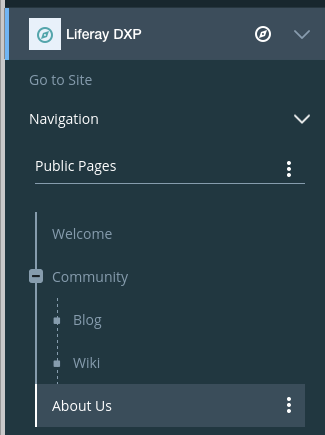
\includegraphics{./images/01-page-hierarchy.png}
\caption{2: Liferay's page hierarchies are easy to create, using a tree
structure that's familiar to anyone who has used a file manager.}
\end{figure}

These pages can have any layout you like: Liferay DXP ships with several
built-in, and you can create your own custom layouts and deploy them
easily. Pages can be added, removed, or reordered any time, and you have
the full flexibility of all the HTML page attributes, such as meta tags
and robot file declarations, that you need.

Pages are also integrated with Liferay's powerful permissions system, so
it's easy to restrict access to certain portions of your site. You can
give individual users sites of their own, with public pages that have
their content and blog, and private pages that contain their calendars
and email.

If you're running a large website that has lots of different sub-sites
for individuals and groups, you can use page templates and site
templates. The former enables you to set up templates of pages with
predefined layouts and applications already on them, and the latter
enables you to create a whole site made up of multiple, predefined
pages.

There's even more. If you have a very large site, you might need
multiple people to work on it. And you certainly don't want the live
site changing before your users' eyes. For that reason, Liferay DXP
provides a feature called \emph{staging} that lets you place your
changes in a holding area while they're being worked on. You can have a
local staging server, where the staged site resides on the same server
as the live site, or you can have a remote staging server, where all web
content work happens on a separate server from your live site. In either
case, when you're ready, site changes can be pushed to the live site,
either manually or on a schedule.

\begin{figure}
\centering
\includegraphics{./images/web-content-staging-publish.png}
\caption{3: Staging supports publishing manually or on a schedule.}
\end{figure}

Liferay DXP's web content creation tools are easy and intuitive to use
at all levels. If you need only basic content management capabilities
for your site, you can jump right in. You can add new content from the
Add menu and drag it right into place. It's easy to go from this basic
level of content management to more sophisticated levels of
functionality.

For example, suppose you wanted to build a news-oriented site. Most of
the content you'll publish is an article of some kind. Liferay's web
content management system lets you create a \emph{structure} for this,
so that you can capture all the information from your writers that you'd
need in an article. The figure below shows what this structure might
look like to a journalist who'd be entering his or her article into the
system.

\begin{figure}
\centering
\includegraphics{./images/01-content-structure.png}
\caption{4: Structures allow you to specify exactly the type of data
that makes up your content. You can also include tooltips to help your
users understand what each field is for.}
\end{figure}

As you can see, you can use structures to make sure writers provide the
title of the story, what type of story it will be, and the byline (i.e.,
the writer's name). You've made sure that all the relevant information
for the story is captured in the system.

Web content is one example of an \emph{asset}. Assets are meta-data
attached to content types, and that meta-data is used to aggregate
similar assets together in searches or as published content. One way to
do this in the example above is to tag and categorize stories so they
can be found more easily by users.

This is just one example, of course. But the concept is applicable to
any kind of site you'd want to build. For example, if you were building
a site for a zoo, you could use web content structures to help users
enter data about animals in the zoo, such as their common names, their
scientific names, their species, their locations in the wild, and more.

When it comes time to publish content, structures are combined with
\emph{templates}. Templates are instructions for how to display
structures, written in Freemarker, a well-known templating language used
for mixing HTML with programmatic elements. Because of this, templates
are very easy to write and can help you ensure that your site has a
consistent look and feel.

There is much more to web content. You can create abstracts, schedule
when content is published and when it should be taken down (or
reviewed), define related assets, and more.

This is just the web content portion of Liferay's content management
system. Liferay DXP is also great at managing file-based content.

\subsection{Keeping track of documents, images, video, and
more}\label{keeping-track-of-documents-images-video-and-more}

It's rare to find a full-featured content management system in an open
source project. Most of the time, you'll find web content management
systems and file-based content management systems as separate projects.
Liferay DXP, however, provides you with both. As shown above, the web
content management system is as robust as any other you'll find, and its
file-based content management system is the same.

You'll find Liferay's file-based content management system in an
application called \emph{Documents and Media Library}. This application
resides on the Site Administration page or can be added to any page,
and, as shown below, looks very much like the file manager that you're
already familiar with from your operating system.

\begin{figure}
\centering
\includegraphics{./images/01-docs-and-media.png}
\caption{5: Liferay DXP's Documents and Media library was purposefully
designed to be familiar to anyone who uses a computer.}
\end{figure}

Like a file manager, you can browse files and folders in nested
hierarchies. You can also mount other repositories that you might have
in your environment, such as any system that implements Content
Management Interoperability Services (CMIS) or Documentum (enterprise
subscribers only). It provides previews of just about every document
type you can think of. And, like a file manager, you can upload, copy,
and move files between folders by dragging and dropping them. Of course,
if you still want to use your operating system's file manager, you can,
because Liferay's Documents and Media library supports WebDAV, using the
same credentials you use to log in to Liferay.

Liferay DXP's Documents and Media library, however, is much more robust
than a file manager is, because it's a full content management system.
You can define ways of classifying files that may be of different types,
but are meant for the same, overarching purpose.

For example, \emph{metadata sets} are groups of fields describing
attributes of a file. One that ships with the product is called
\emph{meeting metadata}, and it contains fields such as Meeting Name,
Date, Time, Location, Description, and Participants. This is a generic
set of fields that go together and that you'd want to use as a group.
You can create as many of these as you want.

For files, you can define \emph{document types}. They provide a more
natural way of working with files. For example, you might create a
document type called Meeting Minutes. The file format doesn't matter:
whether it's a Microsoft Word document, an HTML file, or a text file,
the document contains meeting minutes. Once you've created the document
type, you can attach the Meeting Metadata set that contains many of the
fields you'd want, and you can also add extra fields, such as a field
for action items. When users want to add files containing their notes
for meeting minutes, they can also add all the relevant metadata about
the meeting (such as the time, location, and action items). This
captures the context information that goes with the document, and it
provides a much more natural way of working with documents than just
dumping them into a shared file system.

Of course, the system goes much further than this. Folders can be set so
that only certain document types can be added to them. Workflow rules
can also be added to folders to run files through an approval process
that you define. In short, Liferay's file-based content management
system gives you all the features you need to manage and share files in
a group.

Many Liferay DXP users see it as a robust content management system, and
they use it primarily for that purpose. Now, hopefully, you can see why.
We'll cover the system in-depth in the relevant section on the left, but
for now we need to look at some of the other ways you can use Liferay
DXP, starting with its fantastic collaborative tools.

\section{Using Liferay DXP as a collaborative
platform}\label{using-liferay-dxp-as-a-collaborative-platform}

Many sites have grown organically. You may have grown your community by
using separate tools: first a forums application, and then a wiki for
collaborative documentation, and maybe even a chat application. It can
be hard (and error-prone) to integrate all these applications so your
users can use them seamlessly. Thankfully, Liferay includes a suite of
collaborative applications, and they're all integrated together.

Liferay DXP offers every standard collaborative application that's
available. These applications range from personal productivity
applications like a calendar and email, to community-building
applications like message boards, polls, and wikis.

\begin{figure}
\centering
\includegraphics{./images/01-message-boards.png}
\caption{6: Liferay DXP's message boards are as fully featured as any
standalone forum application, with the added benefit that they're
integrated with the rest of the system.}
\end{figure}

This is a suite of integrated applications with all the features of
similar, standalone applications. For example, Liferay DXP's message
boards include categories and subcategories, message threads, captcha,
RSS feeds, email notification, posting via email, and much more. But
more than this, the applications are integrated with the rest of Liferay
DXP's framework. Users log in and their profiles are used automatically
by the message boards and all the other collaborative applications. And
as we'll see later, functionality from the built in applications can be
added to your own to provide features like comments in your own
software, and you don't have to write any code to do it.

Liferay DXP's wiki is another example of a full-featured collaborative
application. It has support for authoring pages in a WYSWYG editor, or
more advanced users can use the easy-to-learn standard Wiki Creole
syntax. The wiki keeps a full history of every change that's been made,
allowing users to revert back to any change. Users can comment on wiki
articles or read them via RSS feeds (just about every Liferay
application supports this). Each site can have one or more wikis, and
each wiki can have one or more top-level nodes.

One important feature of all the collaborative applications--as well as
web content and documents--is the Recycle Bin. If users delete content
that needs to be restored later, you don't have to find it in your
backups: it's in the Recycle Bin.

\begin{figure}
\centering
\includegraphics{./images/recycle-bin-overview.png}
\caption{7: The Recycle Bin can hold any kind of content.}
\end{figure}

Liferay DXP's suite of collaborative applications includes a blog
(complete with blog aggregation features so you can publish multiple
users' blog entries in one place), a chat application for users who are
online at the same time, message boards, a wiki, a knowledge base that
you can use to publish a library of articles, a polling system you can
use to have users vote on certain questions, and personal productivity
applications like a calendar.

Liferay DXP includes every application you'll need to enable users to
collaborate. Next, you'll see how Liferay can host multiple web sites.

\section{Using Liferay as a web
platform}\label{using-liferay-as-a-web-platform}

We can't even begin to imagine what you're thinking of building, but
whatever it is, you're going to put your heart and soul into it.
Building it on Liferay's web platform can give you a leg up. It provides
everything you need to support your application, so you can concentrate
solely on what \emph{you're} building, and not the rest of the features
your users expect to come along with it.

Imagine your application for a moment. Does it require users to register
on your site? Can users comment on content contained in your
application? Is there something that users can tag or categorize? If you
think about the layout of the application, would it benefit from
modularization? Could you make use of a rich JavaScript framework with
many components built into it? How about security--will you need to make
information available to some users, but not to all users? Liferay DXP
has all of this and more available to developers.

Liferay DXP's development framework is a great help when you're building
an application for the web, for mobile, or for anything in between. For
example, bug fixes to your applications are easy to apply, because
Liferay applications are hot deployed to the running server. Liferay's
Marketplace gives you a ready-made shopping center for your
applications. And Liferay's web services and JSON architecture make it
easy for you to share data from your applications with other systems
running on different platforms.

You get all this and much more. It's a very powerful platform, and
certainly worth your investigation. Read the developer section of this
site to learn more.

\subsection{A great integration
platform}\label{a-great-integration-platform}

If you're building an enterprise system, portals were designed in the
first place to be a single point of entry to your users' applications
and content. Since Liferay DXP integrates well with user directories
such as LDAP and Active Directory, along with single sign-on systems
such as SAML and OpenSSO, it fits well into your enterprise systems.
This allows you to use it as an integration platform for existing
applications.

Liferay DXP, since it adheres to the JSR standard for portlets, was
designed from the ground up for application integration. You can add any
application installed on the system to any page in the portal. You can
make use of APIs provided by other systems to integrate their data into
an application window in Liferay. And applications you create with
Liferay's Service Builder framework are web service-enabled from the
start.

\subsection{Hosting multiple sites on Liferay
DXP}\label{hosting-multiple-sites-on-liferay-dxp}

Liferay DXP excels as a multi-site hosting platform. You can use it to
host multiple sites under the same overall architecture, or you could
host several completely different websites based solely on Liferay's
ability to serve multiple instances of itself from the same physical
installation.

In the first scenario, Liferay DXP's Sites architecture lets you create
multiple, different websites that have public and/or private sets of
pages and as many pages within those sets as you'd like. Users can join
and leave open sites with one click. Alternatively, sites can be defined
as restricted or private, and users can't access those unless they're
added by site administrators. All these sites can have canonical domain
names such as baseballcards.liferay.com or progrock.liferay.com.

Using this construct, you can build anything you can imagine. There is
no limit to the number of sites you can have: some Liferay installations
have only one or two, but others have many thousands. For those larger
installations, Liferay DXP contains a complete site membership
management framework that lets administrators manage automatic site
members for groups of users. It really is built to scale to the size you
need.

In the second scenario, Liferay DXP lets you create completely separate
instances of itself from the same installation. Users, groups,
organizations, sites, and roles from each instance are kept completely
separate. If a user registers for a user id on one instance, he or she
would have to register as a new user on one of the other instances.

This lets you host many different, separate websites from one Liferay
DXP installation. Users of each instance have access to the same
powerful content management, collaboration, social, and web development
platform that they'd have if they were operating from a single,
standalone installation.

Let's see how you can customize Liferay DXP so that it looks and
operates exactly the way you've envisioned for your site.

\section{Extending and customizing Liferay for your own
needs}\label{extending-and-customizing-liferay-for-your-own-needs}

Beyond using it as a development platform for new applications, Liferay
DXP has also been designed to be extended and modified. As an open
source project, its source code is available, but Liferay DXP's
developers have designed the product to make it easy to build whatever
you want out of it.

The first (and easiest) way of customizing parts of Liferay DXP is with
Application Display templates. These let you change the way built-in
applications look. For example, if you don't like the Documents and
Media Library's file manager view with large icons, you can create an
Application Display template that shows documents in some other view. If
you don't like the layout of the Blogs application, you can change it so
that it has the look you want.

Liferay DXP goes far beyond this, though. Special software components
called \emph{modules} enable developers to change Liferay's interface
and behavior--without having to modify any of Liferay DXP's source code.
This provides you all the benefits of building your site from scratch,
but without all the effort to actually build from scratch. If you want
to make a change to the user registration screens, add support for a
proprietary single sign-on mechanism that you've written, add a feature
to the message boards application or anything else, you can make those
customizations. And if you're a developer, you know that it's a whole
lot easier to customize something that almost does things exactly the
way you want than it is to write that feature from scratch. With Liferay
DXP, you \emph{can} have your cake and eat it too.

\section{Summary}\label{summary}

So what is Liferay? As you can see, it's hard to describe, because it
does so much. What we've essentially done is say it's a totally awesome
content and document managing, user collaborating, socially enabling,
application developing, corporate integrating, completely customizable
platform for building the Internet. If we'd said that up front, you'd
probably have doubted us. Hopefully now, you can see that it's true.

If you're interested in using Liferay DXP for \emph{your} product,
continue reading. All of these features (and more that we couldn't
mention) are covered here.

\chapter{Building Websites with Liferay Web Experience
Management}\label{building-websites-with-liferay-web-experience-management}

Nowadays, few people build websites using only a text editor because
that still requires a lot of effort. Why do it manually when you can
have the computer do a lot of the work for you? With Liferay Web
Experience Management, you can focus on your site and let Liferay DXP
handle those low-level details. It provides web content management,
document management, and a framework for robust content display and
advanced content creation. With so many features, it's tough to know
where to start. This is a step by step guide to creating content, pages,
and sites, starting with the most basic elements and ending with a
full-featured website.

\begin{figure}
\centering
\includegraphics{./images/001-final-site-preview.png}
\caption{A preview of the final site.}
\end{figure}

You'll start by creating simple content in an empty Liferay DXP bundle.
As you progress, you'll add more complex content using Liferay DXP's
full suite of tools. These tools include web content display, asset
publisher, content display pages, web content structures and templates,
page templates, application display templates, and more.

Let's Go!{}

\chapter{Creating Basic Web Content}\label{creating-basic-web-content}

As soon as Liferay DXP is installed, you have all the tools you need to
build sites and create content. This means you can start right away! The
first thing to learn is the tool into which your creative juices flow:
Liferay DXP's content editor.

To do this, you'll first create a static piece of web content, and then
in a second step, you'll publish it. In five or ten minutes, you'll
already have a good idea how content creation works in Liferay DXP.
What's stopping you?

\href{https://portal.liferay.dev/documents/113763090/113763156/Creating+Content+Exercise+Images.zip}{Download
the necessary files to complete the exercises.}

Let's Go!{}

\section{Initial Setup}\label{initial-setup}

\begin{verbatim}
<p>Creating Basic Web Content<br>Step 1 of 3</p>
\end{verbatim}

Before you get any further you should set your site name. When you start
a new Liferay bundle for the first time, it creates a site with a single
``Welcome'' page. The default name for the Site is ``Liferay,'' but you
can change that by changing the name globally. You can set the name
through the Setup Wizard or through the Control Panel.

\subsection{Changing the Site Name}\label{changing-the-site-name}

Since you're working on the Lunar Resort website, and not Liferay's
website, you should head over to the Control Panel to set your site name
properly.

\begin{enumerate}
\def\labelenumi{\arabic{enumi}.}
\item
  Open the Menu.
\item
  Click on \emph{Control Panel} → \emph{Configuration}
\item
  Select \emph{Instance Settings}.
\end{enumerate}

\begin{figure}
\centering
\includegraphics{./images/001-instance-settings-page.png}
\caption{The Instance Settings page.}
\end{figure}

On the Instance Settings page, you can configure many aspects of your
Liferay Instance, ranging from the site name and logo to authentication
and email configuration. All you're concerned about today is the site
name.

\begin{enumerate}
\def\labelenumi{\arabic{enumi}.}
\item
  Under \emph{General} → \emph{Main Configuration} enter \emph{The Lunar
  Resort} in the \emph{Name} field.
\item
  Scroll down to the bottom and click \emph{Save}.
\item
  Instantly, you should see that ``The Lunar Resort'' has replaced
  ``Liferay'' wherever the site name is referenced.
\end{enumerate}

\begin{figure}
\centering
\includegraphics{./images/001-liferay-to-lunar.png}
\caption{The Instance Settings page.}
\end{figure}

Now that we have that little bit of housekeeping taken care of, you can
continue to create content and build your site!

\section{Using Liferay DXP's Content
Editor}\label{using-liferay-dxps-content-editor}

\begin{verbatim}
<p>Creating Basic Web Content<br>Step 2 of 3</p>
\end{verbatim}

In Liferay DXP, you create content independent of a page and then
publish it on a page. Separating content creation from content display
lets you publish content on multiple pages without recreating it, and
prevents the loss of content if you remove it from a page or delete the
page altogether.

!P\href{https://portal.liferay.dev/documents/113763090/113920063/vid-using-liferays-content-editor-thumbnail.png}{Video
Thumbnail}

It's time to get started:

\begin{enumerate}
\def\labelenumi{\arabic{enumi}.}
\item
  Open the Menu.
\item
  Under the site (\emph{The Lunar Resort}), select \emph{Content} →
  \emph{Web Content}.
\end{enumerate}

\begin{figure}
\centering
\includegraphics{./images/001-web-content-page.png}
\caption{The Web Content page.}
\end{figure}

The Web Content site administration page is the hub for all the content
in the Lunar Resort site. You create, edit, and review content from this
page.

Follow these steps to create some content:

\begin{enumerate}
\def\labelenumi{\arabic{enumi}.}
\item
  Click the \texttt{+} button in the bottom right corner of the screen
  and select \emph{Basic Web Content}.

  This opens up the web content editor. There are many options here, but
  for now pay attention only to the \emph{Title}, \emph{Summary}, and
  \emph{Content} fields:

  \begin{itemize}
  \tightlist
  \item
    \emph{Title}: The content's title
  \item
    \emph{Summary}: The content's summary. This should be a brief
    description of the content.
  \item
    \emph{Content}: The content's body. For example, if the content is
    an image, you add image in this field.
  \end{itemize}
\item
  In the Title field, enter \emph{Lunar Resort Welcome}.
\item
  In the Summary field, enter \emph{Welcome page content for the Lunar
  Resort}.
\end{enumerate}

The Content field hides a great deal of power. It's sort of like a super
hero. Now you'll use it to create your first piece of web content:

\begin{enumerate}
\def\labelenumi{\arabic{enumi}.}
\item
  In the Content field, enter the text \emph{Make Memories at the Lunar
  Resort}.
\item
  Select the text with your cursor.
\item
  In the toolbar that appears above the text, change \emph{Normal} to
  \emph{Heading 1}. This sets the text as a first-level heading. You may
  need to close the menu for the full dialog above the text to be
  visible.

  \begin{figure}
  \centering
  \includegraphics{./images/001-text-options.png}
  \caption{The Content field lets you format text on the fly.}
  \end{figure}
\item
  De-select the text and make a new line.
\item
  Click the plus button and select the image icon.

  \begin{figure}
  \centering
  \includegraphics{./images/001-image-icon.png}
  \caption{To begin adding an image, select the image icon.}
  \end{figure}
\item
  Using drag and drop or the \emph{Select File} button, upload the
  provided \texttt{moon-image1.jpg}. This also adds it to the Document
  Library so that you can re-use it later.
\item
  Click \emph{Add} to add the image to the content.
\item
  If the image must be resized, click it and then drag the corners.
\item
  Click \emph{Publish}. This saves your web content and makes it
  available for display.
\end{enumerate}

Well done! You created the content, but you must still publish it on a
page so users can see it. You'll do this next.

!V\href{https://portal.liferay.dev/documents/113763090/113920063/using-liferays-content-editor.mp4\%7Chttps://portal.liferay.dev/documents/113763090/113920063/using-liferays-content-editor.webm}{Video
Tutorial}

\section{Publishing Basic Content}\label{publishing-basic-content}

\begin{verbatim}
<p>Creating Basic Web Content<br>Step 3 of 3</p>
\end{verbatim}

Before you publish content, it's useful to know the content hierarchy in
Liferay DXP. You can loosely think of this as the scaffolding that
Liferay DXP uses to display content.

\begin{itemize}
\item
  A Site (like The Lunar Resort) contains pages and content.
\item
  Pages contain applications.
\item
  You can publish a site's content in an application on a page in the
  site. For example, the Web Content Display and Asset Publisher
  applications can display a site's content once they're added to a
  page.
\end{itemize}

!P\href{https://portal.liferay.dev/documents/113763090/113920063/vid-publishing-basic-content-thumbnail.png}{Video
Thumbnail}

If you followed the previous steps, you have a site that contains
content and a page. Now you'll publish that content on that page.

\begin{enumerate}
\def\labelenumi{\arabic{enumi}.}
\item
  Return to The Lunar Resort's Welcome page. If you're still on the Web
  Content page after creating the web content in the previous step,
  click \emph{The Lunar Resort} in the top-left corner of the screen.
\item
  Open the \emph{Add} menu. Select \emph{Content} if it's not already
  selected.

  \begin{figure}
  \centering
  \includegraphics{./images/001-add-menu-content.png}
  \caption{The Add menu with your content.}
  \end{figure}
\item
  Drag and drop \emph{Lunar Resort Welcome} onto the page above the
  \emph{Hello World} portlet.
\end{enumerate}

Behind the scenes, Liferay DXP placed your content inside a Web Content
Display application and added that application to the page. You could
have done this manually by adding a Web Content Display application to
the page and then configuring it to display the content. But it's much
easier to let Liferay DXP do it for you!

\begin{figure}
\centering
\includegraphics{./images/001-basic-content-on-page.png}
\caption{Your content on a page.}
\end{figure}

\subsection{Cleanup}\label{cleanup}

You probably noticed a couple of sub-optimal things about your page:
your content's title looks a bit odd, and the Hello World portlet is
unnecessary now that the page has content. You'll fix this now.

\begin{enumerate}
\def\labelenumi{\arabic{enumi}.}
\item
  Mouse over your content to reveal the portlet bar.
\item
  Click the portlet menu icon and select \emph{Look and Feel
  Configuration}.
\item
  Under \emph{Application Decorators} select \emph{Barebone}. This
  removes the content's title, background, and border from the content
  display. Click \emph{Save}.

  \begin{figure}
  \centering
  \includegraphics{./images/001-select-barebone.png}
  \caption{Change the portlet's look and feel.}
  \end{figure}
\item
  Scroll down to the bottom of the page and mouse over the \emph{Hello
  World} portlet.
\item
  Click the portlet menu icon and select \emph{Remove}.
\item
  Click \emph{OK} when asked if you want to remove the component.
\end{enumerate}

Great work! You've created content, displayed it on a page, and done
some basic page management. Now that you know the basics, you'll dig
deeper and create some more pages to fill with content.

!V\href{https://portal.liferay.dev/documents/113763090/113920063/publishing-basic-web-content.mp4\%7Chttps://portal.liferay.dev/documents/113763090/113920063/publishing-basic-web-content.mkv}{Video
Tutorial}

\chapter{Creating a Site}\label{creating-a-site}

Now that you've created basic web content, you're ready for something a
bit more intricate than a single page with a line of text and an image.
In this part of the Learning Path, you'll create more pages (including
nested pages) and use page layouts to customize how those pages show
applications and content. You'll also learn more about adding
applications to pages and how to manage site navigation.

\begin{figure}
\centering
\includegraphics{./images/001-final-site-preview.png}
\caption{A preview of part of the site you'll create.}
\end{figure}

Let's Go!{}

\section{Creating Pages with
Layouts}\label{creating-pages-with-layouts}

\begin{verbatim}
<p>Creating A Site<br>Step 1 of 6</p>
\end{verbatim}

Up to this point everything on the Welcome page stretches the width of
the entire page. You can control this with \emph{page layouts}. For
example, the Welcome page has the simplest possible layout: one column.
Any items in that column take up its full width. You can place anything
above or below but not to the side of any existing item on the page.
Liferay DXP contains other layouts that arrange items into different
numbers of columns and rows. This gives you a great deal of control over
how applications and content appear in your site.

You'll next use layouts to create the Activities and About Us pages for
the Lunar Resort.

\begin{figure}
\centering
\includegraphics{./images/001-final-activities.png}
\caption{The final Activities page.}
\end{figure}

\begin{figure}
\centering
\includegraphics{./images/001-final-about-us.png}
\caption{The final About Us page.}
\end{figure}

\subsection{Creating the Activities
Page}\label{creating-the-activities-page}

As you may be able to tell from the above screenshot, the Activities
page uses a two column layout with a small column on the left and a
large column on the right. Follow these steps to create this page:

\begin{enumerate}
\def\labelenumi{\arabic{enumi}.}
\item
  Open the main menu and expand the \emph{Navigation} menu for \emph{The
  Lunar Resort}.
\item
  In the Navigation menu, click the \emph{Options} button
  (
\includegraphics{./images/icon-options.png}) for \emph{Public
  Pages} and select \emph{Add Public Page}.

  You are now on the page creation form. You can set the page name,
  choose a template or layout, and set several other options.
\item
  Enter \emph{Activities} for the \emph{Name}.
\item
  For the layout, select \emph{2 Columns (30/70)}. This sets the page to
  the two column layout. The smaller left column takes up 30\% of the
  page, and the larger right column takes up 70\% of the page.

  \begin{figure}
  \centering
  \includegraphics{./images/001-add-activities-page.png}
  \caption{Activities page creation.}
  \end{figure}
\item
  Leave the other options on their default settings and click \emph{Add
  Page}.
\end{enumerate}

The Lunar Resort site now contains the Activities page. This page
appears in the navigation, and you can add applications and content to
it just as you would any other page.

\subsection{Creating the About Us
Page}\label{creating-the-about-us-page}

Now you'll create the \emph{About Us} page. Note in the above screenshot
that this page has three columns. Follow these steps to create this
page:

\begin{enumerate}
\def\labelenumi{\arabic{enumi}.}
\item
  In the main menu, expand the \emph{Navigation} menu for \emph{The
  Lunar Resort}.
\item
  In the Navigation menu, click the \emph{Options} button
  (
\includegraphics{./images/icon-options.png}) for \emph{Public
  Pages} and select \emph{Add Public Page}.
\item
  Enter \emph{About Us} for the Name.
\item
  For the layout, select \emph{3 Columns}.
\item
  Leave the other options on their default settings and click \emph{Add
  Page}.
\end{enumerate}

The navigation bar now contains the two new pages that you just created.
Next, you'll create a couple more pages and then arrange their order in
the navigation bar.

\includegraphics{./images/001-page-navigation.png}

\section{Building the Lunar Guides and Book a Trip
Pages}\label{building-the-lunar-guides-and-book-a-trip-pages}

\begin{verbatim}
<p>Creating A Site<br>Step 2 of 6</p>
\end{verbatim}

The Lunar Resort needs two more pages:

\begin{itemize}
\tightlist
\item
  Lunar Guides: A page that lists the guides employed by the Lunar
  Resort.
\item
  Book a Trip: A page for booking a trip to the Lunar Resort.
\end{itemize}

You'll create these pages using the same steps you used to create the
existing pages.

\subsection{Creating the Lunar Guides
Page}\label{creating-the-lunar-guides-page}

\begin{enumerate}
\def\labelenumi{\arabic{enumi}.}
\item
  Open the main menu and expand the \emph{Navigation} menu for \emph{The
  Lunar Resort}.
\item
  In the Navigation menu, click the \emph{Options} button
  (
\includegraphics{./images/icon-options.png}) for \emph{Public
  Pages} and select \emph{Add Public Page}.
\item
  Enter \emph{Lunar Guides} for the Name.
\item
  For the layout, select \emph{3 Columns}.
\item
  Leave the other options on their default settings and click \emph{Add
  Page}.
\end{enumerate}

\subsection{Creating the Book a Trip
Page}\label{creating-the-book-a-trip-page}

\begin{enumerate}
\def\labelenumi{\arabic{enumi}.}
\item
  Open the main menu and expand the \emph{Navigation} menu for \emph{The
  Lunar Resort}.
\item
  In the Navigation menu, click the \emph{Options} button
  (
\includegraphics{./images/icon-options.png}) for Public Pages
  and select \emph{Add Public Page}.
\item
  Enter \emph{Book a Trip} for the Name.
\item
  For the layout, select \emph{1 Column}.
\item
  Leave the other options on their default settings and click \emph{Add
  Page}.
\end{enumerate}

\subsection{Arranging Pages}\label{arranging-pages}

The new pages now appear in the navigation bar with the other pages. If
these pages are out of your preferred order, you can rearrange them via
drag and drop. Rearrange the pages to match this order:

\begin{figure}
\centering
\includegraphics{./images/001-final-menu.png}
\caption{Reorder the pages in the navigation bar.}
\end{figure}

Great! Now that you have your site's pages, you'll add some applications
to them.

\section{Adding Applications to
Pages}\label{adding-applications-to-pages}

\begin{verbatim}
<p>Creating A Site<br>Step 3 of 6</p>
\end{verbatim}

All of a page's functionality comes from applications. This
functionality can be as simple as displaying content, or as complex as
social networking. You create your page's functionality by adding
applications to the page. You'll get started by adding applications to
the Activities and About Us pages.

\subsection{The Activities Page}\label{the-activities-page}

You'll add two Asset Publisher applications to display different assets,
like images, web content articles, or any other kind of content in
Liferay DXP. Follow these steps to add two Asset Publishers to the page:

\begin{enumerate}
\def\labelenumi{\arabic{enumi}.}
\item
  Navigate to the \emph{Activities} page.
\item
  Click the \emph{Add} button
  (\includegraphics{./images/icon-add-app.png}) on the upper
  right and expand the \emph{Applications} → \emph{Content Management}
  category in the menu.
\item
  Drag and drop one Asset Publisher to the page's right column and the
  other to the page's left column.
\end{enumerate}

\begin{figure}
\centering
\includegraphics{./images/001-drag-asset-publisher.png}
\caption{This screenshot shows the Asset Publisher being placed in the
page's right column. The narrow blue bar indicates where the application
will appear when you release the mouse button.}
\end{figure}

\subsection{The About Us Page}\label{the-about-us-page}

To add functionality to the About Us page, you'll add several Web
Content Display applications. Recall that this application displays web
content. You saw it in action when you displayed basic web content in
the previous section of this Learning Path. Follow these steps to add
Web Content Display to the About Us page:

\begin{enumerate}
\def\labelenumi{\arabic{enumi}.}
\item
  Navigate to the \emph{About Us} page.
\item
  Click the \emph{Add} button
  (\includegraphics{./images/icon-add-app.png}) on the upper
  right and expand the \emph{Applications} category in the menu.
\item
  This time use the search bar to search for \emph{web content display}.
\item
  This page's layout has three columns. Drag and drop a Web Content
  Display application into each column.
\end{enumerate}

As you can see, adding content and applications to pages is a matter of
drag and drop. Next, you'll learn about page management and navigation.

\section{Page Templates}\label{page-templates}

\begin{verbatim}
<p>Creating A Site<br>Step 4 of 6</p>
\end{verbatim}

As you've now seen, creating pages can be repetitive. Wouldn't it be
great if you could create multiple pages from a single template? Well
guess what: page templates in Liferay DXP let you do exactly that! They
also inherit future changes to those pages.

Now you'll use page templates in The Lunar Resort. First you'll create a
page template, then you'll use it to create several pages. Later, you'll
make changes to the template and see Liferay DXP propagate those changes
to the pages you created from the template.

\subsection{Creating a Page Template}\label{creating-a-page-template}

Use these steps to create a page template:

\begin{enumerate}
\def\labelenumi{\arabic{enumi}.}
\item
  Open the Main Menu and select \emph{Control Panel} → \emph{Sites} →
  \emph{Page Templates}. The Page Templates page lists all the page
  templates in the Liferay DXP instance. Three page templates come
  bundled with Liferay DXP. \emph{Blog} and \emph{Wiki} are example
  layouts for the Blogs and Wiki applications. \emph{Content Display
  Page} serves a special function that you'll work with later.

  \begin{figure}
  \centering
  \includegraphics{./images/001-page-templates-screen.png}
  \caption{The Page Templates page.}
  \end{figure}
\item
  Click the \emph{Add} button
  (
\includegraphics{./images/icon-add.png}) in the lower right
  corner. This takes you to the page template creation page.
\item
  Name the template \emph{Lunar Guide Page}.
\item
  For the description, enter \emph{Page with information about a Lunar
  Guide}.
\item
  Click \emph{Save}. This takes you back to the list of page templates,
  where you can see the new template in the list.
\end{enumerate}

\subsection{Editing a Page Template}\label{editing-a-page-template}

Editing a page template is similar to editing any page. You drag and
drop applications onto the page and reposition or remove them as
desired. The only difference is that you can't directly add content, and
some configuration and display options are disabled (it's a template,
after all). Follow these steps to edit the page template you just
created:

\begin{enumerate}
\def\labelenumi{\arabic{enumi}.}
\item
  In the list of page templates, click \emph{Lunar Guide Page}. This
  opens it in a new browser tab or window.

  \begin{figure}
  \centering
  \includegraphics{./images/001-lunar-resort-template-edit.png}
  \caption{Click the page template to edit it.}
  \end{figure}
\item
  In the page template's edit toolbar click the \emph{Add} button
  (\includegraphics{./images/icon-add-app.png}) on the upper
  right and expand the \emph{Applications} → \emph{Collaboration}
  category. Add a Blogs portlet to the page template's right column.
\item
  Close the page template's edit tab/window. Liferay DXP automatically
  saves your changes.
\end{enumerate}

Next, you'll create a page with this template.

\subsection{Creating a Page with a Page
Template}\label{creating-a-page-with-a-page-template}

Follow these steps to use the template to create a page:

\begin{enumerate}
\def\labelenumi{\arabic{enumi}.}
\item
  Open the Main Menu and select \emph{The Lunar Resort} →
  \emph{Navigation}.
\item
  In the Navigation menu, click the \emph{Options} button
  (
\includegraphics{./images/icon-options.png}) for \emph{Public
  Pages} and select \emph{Add Public Page}.
\item
  Name the page \emph{Cody} (Cody is one of our lunar guides).
\item
  Under \emph{Type}, select \emph{Lunar Guide Page}. This selects your
  page template as the source for the page.
\item
  Leave \emph{Inherit Changes} set to \emph{Yes}. This lets you edit
  this page in the future by editing the template, but removes the
  ability to edit the page directly.
\item
  Click \emph{Add Page}.
\end{enumerate}

Liferay DXP then creates the new page from your template. Next, you'll
create more of these pages, one for each lunar guide (Cody is awesome,
but he can't do everything by himself). Note, however, that Cody's page
is in the navigation bar next to all the other pages. To get his page
and those of the other lunar guides under the Lunar Guides page, you
must nest the pages. You'll learn how to do this next.

\section{Nesting Pages}\label{nesting-pages}

\begin{verbatim}
<p>Creating A Site<br>Step 5 of 6</p>
\end{verbatim}

When creating sites, you'll likely encounter situations where you want
to nest pages under other pages. Such child pages (also called nested
pages) let you create page hierarchies to organize content and
functionality. For example, the pages for each lunar guide should be
nested under the Lunar Guides page. Although this is a simple use case,
note that pages in Liferay DXP can be nested to unlimited levels. This
lets your site support even the most demanding hierarchies, so long as
you can design a UI to handle it.

In this article, you'll nest the existing lunar guide page for Cody
under the Lunar Guides page. You'll then create more lunar guide pages
as child pages of the same Lunar Guides page.

\subsection{Creating Child Pages}\label{creating-child-pages}

There are two ways to create a child page in Liferay DXP:

\begin{enumerate}
\def\labelenumi{\arabic{enumi}.}
\item
  Create a new page as a child page of an existing page. This is the
  most common way.
\item
  Turn an existing page into a child page of another existing page. You
  can even do this via drag and drop.
\end{enumerate}

You'll start with the second option, since you already created a page
(Cody) that you want to nest under the Lunar Guides page.

\paragraph{Creating Child Pages with Drag and
Drop}\label{creating-child-pages-with-drag-and-drop}

Using a site's \emph{Navigation} menu, you can nest pages via drag and
drop. Liferay DXP immediately applies any changes you make here to the
site's navigation structure. Follow these steps to nest the \emph{Cody}
page under the \emph{Lunar Guides} page:

\begin{enumerate}
\def\labelenumi{\arabic{enumi}.}
\item
  Open the Main Menu and select \emph{Lunar Resort} → \emph{Navigation}.
\item
  Drag and drop the page \emph{Cody} and so that it nests under the
  \emph{Lunar Guides} page.

  \begin{figure}
  \centering
  \includegraphics{./images/001-drag-cody.png}
  \caption{Nesting a page with drag and drop.}
  \end{figure}
\item
  Refresh the page. The new page hierarchy now appears in the navigation
  bar.

  \begin{figure}
  \centering
  \includegraphics{./images/001-nav-hierarchy-1.png}
  \caption{The page \emph{Cody} is now nested under \emph{Lunar Guides}
  page.}
  \end{figure}
\end{enumerate}

Nice work! Next, you'll create the rest of the pages for the lunar
guides as child pages of the \emph{Lunar Guides} page. Cody is about to
have some company.

\paragraph{Creating New Child Pages}\label{creating-new-child-pages}

The Lunar Resort's other lunar guides--Jim, Steve, and Russ--also need
pages nested under the \emph{Lunar Guides} page. You'll create these
pages directly as child pages:

\begin{enumerate}
\def\labelenumi{\arabic{enumi}.}
\item
  In the \emph{Lunar Resort} → \emph{Navigation} menu, click the
  \emph{Options} button
  (
\includegraphics{./images/icon-options.png}) for \emph{Lunar
  Guides} and select \emph{Add Child Page}.
\item
  Name the page \emph{Jim} and set its type as \emph{Lunar Guide Page}.
\item
  Leave \emph{Inherit Changes} set to \emph{YES}, and click \emph{Add
  Page}.
\item
  Repeat these steps to create pages for Steve and Russ.
\end{enumerate}

Liferay DXP creates each page from the template, with the Blogs app in
the right column and an empty space in the left column. Each page also
appears in the navigation bar under the \emph{Lunar Guides} page.

\begin{figure}
\centering
\includegraphics{./images/001-all-nested-pages.png}
\caption{Cody is no longer lonely!}
\end{figure}

Now that you've created all the pages, you'll learn more about site
navigation and the various features of Liferay's Breadcrumb and
Navigation apps.

\section{Site Navigation}\label{site-navigation}

\begin{verbatim}
<p>Creating A Site<br>Step 6 of 6</p>
\end{verbatim}

You could have the greatest site in the multi-verse, but if users can't
navigate it, it's all for naught. Fortunately Liferay DXP provides
extensive support for customizing your site's navigation. There are two
main ways to define and customize site navigation:

\begin{enumerate}
\def\labelenumi{\arabic{enumi}.}
\item
  In the site's theme. This is the primary and most powerful way to
  manage site navigation. Themes in Liferay DXP can customize any aspect
  of a site, including its navigation. Defining site navigation in the
  theme provides a uniform look and feel across the site.
\item
  With apps. Navigation apps can define navigation on a page-by-page
  basis. For example, the Navigation Menu app displays a navigable page
  hierarchy of the site. You can select which page in the hierarchy to
  use as the root. There's also the Breadcrumb app, which displays the
  trail of pages in the hierarchy that lead to the current page. Like a
  trail of breadcrumbs in the woods, this app lets users retrace their
  steps so they don't get lost.
\end{enumerate}

These two ways of defining site navigation can be used together. Like
page templates, themes can define which apps appear in a site. You've
already seen an example of this in action without being aware of it. The
Lunar Resort uses the Liferay DXP's default theme, Classic. This theme
embeds the Navigation Menu app as the site navigation bar. Therefore,
the Lunar Resort's navigation bar is nothing more than a Navigation Menu
app configured to display the entire site's page hierarchy.

You won't change the theme the Lunar Resort uses, but you'll fine-tune
the site's navigation by adding another Navigation Menu app and a
Breadcrumb app.

\subsection{Adding a Navigation Menu
App}\label{adding-a-navigation-menu-app}

The current Navigation Menu app does a fine job of defining the Lunar
Resort's navigation bar, so why would you want to add another one? For
footer navigation, of course! Once a page requires scrolling, the
navigation bar disappears. It's therefore useful to have another one at
the bottom of the page. Follow these steps to add and configure such a
Navigation Menu app:

\begin{enumerate}
\def\labelenumi{\arabic{enumi}.}
\item
  Go to the Lunar Resort's \emph{Welcome} page.
\item
  Click the \emph{Add} button
  (\includegraphics{./images/icon-add-app.png}) on the upper
  right and expand the \emph{Applications} → \emph{Content Management}
  category in the menu.
\item
  Drag a \emph{Navigation Menu} app onto the page below the existing
  content.
\item
  Mouse over the Navigation Menu app and click the app's \emph{Options}
  menu (\includegraphics{./images/icon-app-options.png}) on the
  right hand side of the portlet bar. Then select \emph{Look and Feel
  Configuration}.
\item
  Set \emph{Application Decorators} to \emph{Barebone}, click
  \emph{Save}, then close the dialog box.
\item
  Now select \emph{Configuration} from the Navigation Menu app's
  \emph{Options} menu
  (\includegraphics{./images/icon-app-options.png}).
\item
  For \emph{Display Template}, select \emph{Bar minimally justified
  styled}.
\item
  Leave the rest of the default settings alone, then click \emph{Save}
  and close the dialog box.
\end{enumerate}

The navigation footer should look like this:

\begin{figure}
\centering
\includegraphics{./images/001-nav-footer.png}
\caption{The Welcome page now has a navigation footer.}
\end{figure}

Great! Next, you'll add a Breadcrumb app.

\subsection{Adding a Breadcrumb App}\label{adding-a-breadcrumb-app}

To add the Breadcrumb app, you'll leverage the power of Page Templates.
Recall that you created the Lunar Guide pages using a template with the
Blogs app in the right hand column of the page. Since Liferay DXP
propagates template changes to the pages, you'll now change the template
to add a Breadcrumb app to each of the Lunar Guide pages. Follow these
steps to do so:

\begin{enumerate}
\def\labelenumi{\arabic{enumi}.}
\item
  Open the Main Menu and select \emph{Control Panel} → \emph{Sites} →
  \emph{Page Templates}.
\item
  In the list of page templates, click \emph{Lunar Guide Page}.
\item
  Add a \emph{Breadcrumb} application from the Content Management
  category to the page template's left column (next to the Blogs
  application).
\item
  Open Breadcrumb app's \emph{Options} menu
  (\includegraphics{./images/icon-app-options.png}) and select
  \emph{Look and Feel Configuration}.
\item
  Change \emph{Application Decorators} to \emph{Barebone}, then click
  \emph{Save} and close the dialog.
\item
  Close the page template editing tab/window.
\item
  Navigate to one of the lunar guide pages. The Breadcrumb now appears
  alongside the Blogs app.

  \begin{figure}
  \centering
  \includegraphics{./images/001-breadcrumb-jim.png}
  \caption{After adding the Breadcrumb app to the page template, the app
  appears on each lunar guide page, to the left of the Blogs app.}
  \end{figure}
\end{enumerate}

As you've seen, the Navigation Menu and Breadcrumb apps help users
traverse page hierarchies. These apps are invaluable for any site with
complex page hierarchies.

Awesome! Now that you've created your site's framework with pages and
navigation, you'll fill the site with content.

\chapter{Creating Content}\label{creating-content}

So far you've created the Lunar Resort site's outline. By creating pages
and using templates, the site now has a structure and the pages have
layouts. Now it's time to color everything in with content.

In this section you'll create content, some with more complex web
content structures and templates, and use Liferay's Web Experience
Management to publish your new content on your site.

\begin{figure}
\centering
\includegraphics{./images/001-more-basic-content.png}
\caption{Basic web content.}
\end{figure}

\begin{figure}
\centering
\includegraphics{./images/001-adt-content.png}
\caption{Application Display Template.}
\end{figure}

Let's Go!{}

\section{Creating More Content}\label{creating-more-content}

\begin{verbatim}
<p>Creating Content<br>Step 1 of 7</p>
\end{verbatim}

Earlier we created some content without knowing where it would go. Now
you have the context of how the site is organized. Next, use the same
principles for creating content on the front page to create articles for
the \emph{About Us} page.

On the \emph{About Us} page, you'll add information about the Lunar
Resort and other related Space Program initiatives.

\subsection{Creating the About Us Page
Content}\label{creating-the-about-us-page-content}

Recall that you created the Welcome page's content in Site
Administration and then added it to the page. You'll use a slightly
different method to create the About Us page's content. Specifically,
you'll use the Web Content Display app to create the content directly in
that app.

\begin{enumerate}
\def\labelenumi{\arabic{enumi}.}
\item
  Go to the \emph{About Us} page.
\item
  In the portlet bar of the left column's Web Content Display app, click
  the \emph{Add} button
  (\includegraphics{./images/icon-portlet-add-control.png}) and
  select \emph{Basic Web Content}. This takes you to the app's web
  content creation page. The content you create here only appears in
  this app, on this page.

  \begin{figure}
  \centering
  \includegraphics{./images/001-content-on-page.png}
  \caption{You can create basic web content directly in the Web Content
  Display app.}
  \end{figure}
\item
  Enter the following information for the following fields:

  \begin{itemize}
  \tightlist
  \item
    \textbf{Title:} The Lunar Resort
  \item
    \textbf{Summary:} Information about the Lunar Resort
  \item
    \textbf{Content}: The Lunar Resort is an all-inclusive, one of a
    kind vacation spot with attractions and activities unlike anything
    you've ever seen or done before.
  \end{itemize}
\item
  With your cursor still in the Content field one line below the text
  you just entered, click the plus button and select the image icon.
  Select \texttt{lunar-resort-logo.png}.
\item
  Resize the image if necessary, then click \emph{Publish}.
\end{enumerate}

The Web Content Display app in the left column now contains your
content.

To add content in the remaining Web Content Display apps, repeat the
above steps for each app but add different information in step two, and
a different image in step three.

\begin{enumerate}
\def\labelenumi{\arabic{enumi}.}
\item
  Add this for the Web Content Display app in the middle column:

  \begin{itemize}
  \tightlist
  \item
    \textbf{Title:} The Space Program
  \item
    \textbf{Summary:} Information about the Space Program
  \item
    \textbf{Content:} The Space Program is our parent company and
    contains our research, development, and exploration divisions. You
    can learn more about the Space Program here.
  \item
    Add the image \texttt{space-program-logo.png}.
  \end{itemize}
\item
  Add this for the Web Content Display app in the right column:

  \begin{itemize}
  \tightlist
  \item
    \textbf{Title:} S.P.A.C.E.
  \item
    \textbf{Summary:} Information about S.P.A.C.E.
  \item
    \textbf{Content:} The Space Program Academy of Continuing Education
    (S.P.A.C.E.) is the Space Program's educational wing. You can visit
    its lunar campus during your Lunar Resort stay.
  \item
    Add the image \texttt{space-logo.png}.
  \end{itemize}
\end{enumerate}

Great! The About Us page is now complete and provides all the
information that the Lunar Resort's visitors need.

\begin{figure}
\centering
\includegraphics{./images/001-final-about-us.png}
\caption{The complete About Us page looks awesome!}
\end{figure}

Next, you'll learn how to use Liferay DXP's Documents and Media features
to manage files in your portal.

\section{Using Documents and Media}\label{using-documents-and-media}

\begin{verbatim}
<p>Creating Content<br>Step 2 of 7</p>
\end{verbatim}

Liferay DXP's Documents and Media features provide tools for uploading,
organizing, and displaying various types of documents and media,
including images, audio, and video. For example, you can use Documents
and Media for collaborating on files like text documents or
spreadsheets, managing collections of images, or simply storing the
images that your web content references.

You've been using Documents and Media without knowing it. The images you
added when creating web content were automatically added to the
Documents and Media library. But there's a more efficient way to add
images to Documents and Media. You can add many images at once, directly
in the Documents and Media library. This saves you a step when creating
content that uses those images. Working directly in the Documents and
Media library also lets you organize your files in folders just as you
would on a traditional desktop environment.

Now you'll take advantage of these features in the Lunar Resort.

\subsection{Adding Files}\label{adding-files}

You still need to create more content in the Lunar Resort, and this
content needs images. You'll upload all these images now in the
Documents and Media library:

\begin{enumerate}
\def\labelenumi{\arabic{enumi}.}
\item
  Open the \emph{Menu} (
\includegraphics{./images/icon-menu.png})
  and select \emph{The Lunar Resort} → \emph{Content} → \emph{Documents
  and Media}. The Documents and Media screen appears and displays the
  Documents and Media library's Home folder (its root folder). Note that
  the images you added while creating content earlier are all here.

  \begin{figure}
  \centering
  \includegraphics{./images/001-existing-images.png}
  \caption{The Documents and Media library's Home folder contains the
  Lunar Resort's existing images.}
  \end{figure}
\item
  Click the \emph{Add} icon
  (\includegraphics{./images/icon-add.png}) at the bottom-right
  of the page and select \emph{Multiple Documents}.
\item
  Use the \emph{Add Multiple Documents} screen to add the images
  \texttt{moon-image1.jpg}, \texttt{moon-image2.jpg},
  \texttt{moon-image3.jpg}, \texttt{booking-image.png},
  \texttt{guide-cody.png}, \texttt{guide-jim.png},
  \texttt{guide-russ.png}, and \texttt{guide-steve.png}. You can either
  drag and drop the files from your file system to the box, or click
  \emph{Select Files} to select the files via a file manager window. If
  you wish, you can also categorize and describe the files. Click
  \emph{Publish} to complete the upload.

  \begin{figure}
  \centering
  \includegraphics{./images/001-add-multiple-documents.png}
  \caption{The Documents and Media library lets you add multiple
  documents at once.}
  \end{figure}
\end{enumerate}

Great! The Lunar Resort's Documents and Media library now contains more
images--enough to warrant organizing them in folders.

\subsection{Adding Folders}\label{adding-folders}

Your Documents and Media library is now a bit more crowded. It's time to
organize it with folders. Besides basic file organization, you can also
use folders for managing access to files via permissions.

Follow these steps to add some folders to the Lunar Resort's Documents
and Media library:

\begin{enumerate}
\def\labelenumi{\arabic{enumi}.}
\item
  Return to the Documents and Media library's Home folder.
\item
  Click the \emph{Add} icon
  (\includegraphics{./images/icon-add.png}) at the bottom-right
  of the page and select \emph{Folder}.
\item
  Name the folder \emph{Web Content Images}, and give it the description
  \emph{Images used in Lunar Resort Web Content}.
\item
  Click \emph{Save}. This returns you to the Documents and Media
  library's Home folder, where your new folder is now available.
\item
  Repeat the steps above to folders named \emph{Frontpage Images} and
  \emph{Lunar Guides} to the Home folder.
\end{enumerate}

Sweet! The Lunar Resort's Documents and Media library now contains two
folders. You'll use them to organize images next.

\subsection{Organizing Media}\label{organizing-media}

Before moving your files into the new folders, it's important to know
that you can move files that are currently in use, without issue. For
example, if a piece of web content uses an image, and you move that
image to a different Documents and Media folder, you don't need to
update that web content with the image's new location. Liferay DXP
maintains such file connections for you.

Follow these steps to move files to your new folders:

\begin{enumerate}
\def\labelenumi{\arabic{enumi}.}
\item
  Return to the Documents and Media library's Home folder and check the
  boxes on the images \texttt{lunar-resort.png}, \texttt{space.png}, and
  \texttt{space-program.png}.
\item
  Drag and drop the selected images to the Web Content Images folder.

  \begin{figure}
  \centering
  \includegraphics{./images/001-drag-files.png}
  \caption{The Documents and Media library lets you drag and drop files
  into a folder.}
  \end{figure}
\item
  The next screen lets you review and confirm the move. It also lets you
  change which files are included, and their destination. Leave the
  default selections and click \emph{Move}.
\item
  Repeat these steps to move the guide images to the \emph{Lunar Guides}
  folder and the Home folder's remaining files to the \emph{Frontpage
  Images} folder.
\end{enumerate}

Well done! Now your Documents and Media library contains the images you
need for creating more content. You also learned how to upload and
manage files in Documents and Media. Next, you'll learn about creating
more complex content and styles using structures and templates.

\chapter{Web Content Structures and
Templates}\label{web-content-structures-and-templates}

\begin{verbatim}
<p>Creating Content<br>Step 3 of 7</p>
\end{verbatim}

In Liferay DXP, you can use \emph{structures} and \emph{templates} to
create new web content types and layouts. A structure defines the type
of items in your content, such as text, images, calendar items,
checkboxes, links, and more. Structures are based on Liferay DXP's forms
functionality. When creating content based on a structure, you must fill
out that structure's fields.

A template uses a templating language to display a structure's items, so
you can apply styles and logic to create complex or interactive content.
You can create templates in \href{http://freemarker.org/}{FreeMarker} or
\href{http://velocity.apache.org/}{Velocity}. Templates can contain CSS,
HTML, JavaScript, and elements of the templating language it uses.

Before getting started with structures and templates, you should know
something important: you've actually already used them! Basic Web
Content is a type of web content defined by a structure and a template.
Now you'll use structures and templates to create something a little
more intricate.

\begin{figure}
\centering
\includegraphics{./images/001-content-template-example.png}
\caption{Content using a template.}
\end{figure}

Let's Go!{}

\section{Creating Structures}\label{creating-structures}

\begin{verbatim}
<p>Creating Content<br>Step 3A of 3D</p>
\end{verbatim}

Now you'll create your first structure. This structure defines Lunar
Guides page content: a picture of the guide along with the guide's name
and a link to his personal page.

\subsection{Creating Your First
Structure}\label{creating-your-first-structure}

\begin{enumerate}
\def\labelenumi{\arabic{enumi}.}
\item
  Open the \emph{Menu}
  (\includegraphics{./images/icon-menu.png}) and select
  \emph{The Lunar Resort} → \emph{Content} → \emph{Web Content}.
\item
  At the top-right, select \emph{Options}
  (\includegraphics{./images/icon-options.png}) →
  \emph{Structures} to see a list of the available structures.
  Currently, only the default Basic Web Content structure is available.

  \begin{figure}
  \centering
  \includegraphics{./images/001-select-structures.png}
  \caption{Select \emph{Structures} from the \emph{Options} menu.}
  \end{figure}
\item
  Click the \emph{Add} icon
  (\includegraphics{./images/icon-add.png}) at the
  bottom-right of the page to begin creating a new structure.
\item
  Name the structure \emph{Lunar Guides List}.
\item
  Now you're ready to define the structure's fields. You do this by
  dragging and dropping the available field types from the \emph{Fields}
  tab to the blank canvas on the right.

  \begin{figure}
  \centering
  \includegraphics{./images/001-structure-fields.png}
  \caption{These fields are available when creating a structure.}
  \end{figure}

  This structure needs a Text field for a title, another Text field for
  the guide's name, an Image field for the guide's image, and a Link to
  Page field for the link to the guide's personal page. Follow these
  instructions to add these fields:

  \begin{itemize}
  \tightlist
  \item
    Drag a \emph{Text} field onto the canvas.
  \item
    Drag another \emph{Text} field onto the canvas, below the first one.
  \item
    Drag an \emph{Image} field into the second Text field, to nest it
    under that Text field. This creates a \emph{field group}.
  \item
    Drag a \emph{Link to Page} field into the field group, below the
    Image field. Be careful to position this Link to Page field so that
    it's on the same level as the Image field (not nested in the Image
    field).
  \end{itemize}

  \begin{figure}
  \centering
  \includegraphics{./images/001-structure-group.png}
  \caption{The canvas should look like this after you add the Text,
  Image, and Link to Page fields. Note that the Image and Link to Page
  fields are nested in the second Text field.}
  \end{figure}
\item
  Click the first Text field. The available fields list is replaced with
  a list of settings for the selected field. Change the following
  settings:

  \begin{itemize}
  \tightlist
  \item
    \textbf{Field Label:} This is the field's title that users see when
    creating content with this structure. Set this to \emph{Title}.
  \item
    \textbf{Name:} This is the field's internal name that you can access
    in a template. Set this to \emph{title}.
  \end{itemize}
\item
  Click the second Text field. Change its \emph{Field Label} to
  \emph{Lunar Guide Name}, and its \emph{Name} to \texttt{name1}.
\item
  Click the \emph{Image} field. Change its \emph{Name} to
  \texttt{image1}.
\item
  Click the \emph{Link to Page} field. Change its \emph{Name} to
  \texttt{link1}.
\item
  There are four lunar guides, so you need four field groups.
  Fortunately, you don't have to create each additional field group
  manually. Hover over the Lunar Guide Name field and click the
  \emph{Duplicate} button
  (\includegraphics{./images/icon-add-2.png}) that appears to
  the field's right. This duplicates the entire field group. Click this
  button two more times until you have a total of four identical field
  groups.
\end{enumerate}

\noindent\hrulefill

\begin{verbatim}
 **Note:** Instead of duplicating fields, you could have used each field's
 *Repeatable* option. This lets users decide how many fields or field groups
 to use when they create content. This is a more advanced option that you'll
 learn about later.
\end{verbatim}

\noindent\hrulefill

\begin{enumerate}
\def\labelenumi{\arabic{enumi}.}
\setcounter{enumi}{10}
\item
  Now you'll change the duplicate fields' names. Repeat steps 7 through
  9 above for each duplicate field group, matching the digit in each
  field name to the field group's number. For example, name the second
  field group's \emph{Name}, \emph{Image}, and \emph{Link to Page}
  fields \texttt{name2}, \texttt{image2}, and \texttt{link2},
  respectively. Likewise, the digit in each field name should be
  \emph{3} for the third field group, and \emph{4} for the fourth field
  group.
\item
  Click \emph{Save}.
\end{enumerate}

Great! Next, you'll create the template to go along with this structure.

\section{Creating Templates}\label{creating-templates}

\begin{verbatim}
<p>Creating Content<br>Step 3B of 3D</p>
\end{verbatim}

Structures, like the one you created in the previous step, need
templates to style and display their items. Now you'll use the
\href{http://freemarker.apache.org/}{FreeMarker} templating language to
create a template.

Follow these steps to create your template:

\begin{enumerate}
\def\labelenumi{\arabic{enumi}.}
\item
  Open the \emph{Menu}
  (\includegraphics{./images/icon-menu.png}) and select
  \emph{The Lunar Resort} → \emph{Content} → \emph{Web Content}.
\item
  At the top-right of the screen, select \emph{Options}
  (\includegraphics{./images/icon-options.png}) →
  \emph{Templates}.
\end{enumerate}

\begin{figure}
\centering
\includegraphics{./images/001-menu-templates.png}
\caption{Select Templates from the menu.}
\end{figure}

\begin{enumerate}
\def\labelenumi{\arabic{enumi}.}
\setcounter{enumi}{2}
\item
  Click the \emph{Add} icon
  (\includegraphics{./images/icon-add.png}) at the
  bottom-right of the page to begin creating a new template.
\item
  Name the template \emph{Lunar Guides List}.
\item
  Now you must select a structure to link with this template. Open the
  \emph{Details} section, click the \emph{Select} button under
  \emph{Structure}, and select the \emph{Lunar Guides List} structure.
  Click \emph{OK} when prompted.
\end{enumerate}

\begin{figure}
\centering
\includegraphics{./images/001-template-details.png}
\caption{Template details.}
\end{figure}

\begin{enumerate}
\def\labelenumi{\arabic{enumi}.}
\setcounter{enumi}{5}
\item
  Next, select the template's language. Still in the Details section,
  make sure \emph{FreeMarker} is selected for the Language field (it
  should be selected by default). FreeMarker uses the FreeMarker
  Template Language (FTL), which uses HTML, interpolations
  (\texttt{\$\{...\}}), and FTL tags. FreeMarker templates can also
  include CSS. For more information on FTL, see
  \href{http://freemarker.apache.org/docs/dgui_quickstart_template.html}{the
  FreeMarker documentation}. Note that Liferay DXP also supports
  Velocity and Extensible Stylesheet Language.
\item
  Now you're ready to create the script. First you'll insert the CSS.
  This example uses a four column, two row grid layout to define the
  field positions. The content appears only in columns two and four--the
  other two columns exist for spacing. This example also defines the
  text heading styles. In the \emph{Script} section, replace the code in
  the editor with this code:

\begin{verbatim}
<style>
   .wrapper {
  display: grid;
  grid-template-columns: 300px, 300px, 300px, 300px;
  grid-gap: 10px;
  grid-auto-rows: minmax(auto, auto);
  text-align: center;
}

h1 {
    text-align: center;
}

h2 { 
   position: relative;
   color: black;
}

.item-one {
  grid-column: 2;
  grid-row: 1;
  max-width: 355px;
}

.item-two { 
  grid-column: 4;
  grid-row: 1;
  max-width: 355px;
}

.item-three {
  grid-column: 2;
  grid-row: 2;
  max-width: 355px;
}

.item-four {
  grid-column: 4;
  grid-row: 2;
  max-width: 355px;
}
</style>    
\end{verbatim}
\item
  Now you're ready to create the template's HTML. Like the structure,
  you can use the sidebar to the editor's left to insert fields in the
  editor. Doing so automatically inserts fields with the appropriate
  variables. \emph{General Variables} provides quick access to universal
  information for your Liferay DXP instance. \emph{Fields} provides
  access to the variables that your structure defines. Mousing over a
  field displays its variable name. Clicking a field adds the code in
  the editor that retrieves that field's data.

  \begin{figure}
  \centering
  \includegraphics{./images/001-field-mouse-over.png}
  \caption{A field's tooltip shows that field's variable name.}
  \end{figure}

  In this example, however, you'll copy and paste the following code.
  This code gets the field values that the user entered, styles the text
  and images, and puts all the information into divs as defined in your
  CSS. Add this code in the editor, below the closing
  \texttt{\textless{}/style\textgreater{}} tag:

\begin{verbatim}
<h1>${title.getData()}</h1>

<div class="wrapper">
  <a class="item-one" href="${name1.link1.getFriendlyUrl()}">
  <h2>${name1.getData()}</h2>
    <#if name1.image1.getData()?? && name1.image1.getData() != "">
      <img alt="${name1.image1.getAttribute("alt")}" src="${name1.image1.getData()}" />
    </#if>
  </a>

  <a class="item-two" href="${name2.link2.getFriendlyUrl()}">
  <h2>${name2.getData()}</h2>
    <#if name2.image2.getData()?? && name2.image2.getData() != "">
      <img alt="${name2.image2.getAttribute("alt")}" src="${name2.image2.getData()}" />
    </#if>
  </a>

<hr />

  <a class="item-three" href="${name3.link3.getFriendlyUrl()}">
  <h2>${name3.getData()}</h2>
    <#if name3.image3.getData()?? && name3.image3.getData() != "">
      <img alt="${name3.image3.getAttribute("alt")}" src="${name3.image3.getData()}" />
    </#if>
  </a>

  <a class="item-four" href="${name4.link4.getFriendlyUrl()}">
  <h2>${name4.getData()}</h2>
    <#if name4.image4.getData()?? && name4.image4.getData() != "">
      <img alt="${name4.image4.getAttribute("alt")}" src="${name4.image4.getData()}" />
    </#if>
  </a>

</div>
\end{verbatim}
\item
  Click \emph{Save}.
\end{enumerate}

Great! Now you have a template for displaying your structure's items.
Next, you'll create some content that leverages your structure and
template.

\section{Creating Content with Structures and
Templates}\label{creating-content-with-structures-and-templates}

\begin{verbatim}
<p>Creating Content<br>Step 3C of 3D</p>
\end{verbatim}

Now that you have a template for your structure, you can use that
structure to create content. Remember, the template formats the
structure's content for display.

Follow these steps to create your content:

\begin{enumerate}
\def\labelenumi{\arabic{enumi}.}
\item
  Open the \emph{Menu}
  (\includegraphics{./images/icon-menu.png}) and select
  \emph{The Lunar Resort} → \emph{Content} → \emph{Web Content}.
\item
  Click the \emph{Add} icon
  (\includegraphics{./images/icon-add.png}) at the
  bottom-right of the page and select \emph{Lunar Guides List}. This
  takes you to the New Web Content form for your structure. Note that
  the fields and field groups you defined in the structure are all here.
\item
  For both \emph{Title} fields, enter \emph{Choose Your Lunar Guide}.
  Don't worry about the duplication. The first Title field is default
  for all web content. You'll use the Web Content Display app to show
  only your structure's title field. This lets you use the template to
  style the field's content, rather than apps that display web content.
\item
  Fill out a field group for each lunar guide: \emph{Cody}, \emph{Jim},
  \emph{Russ}, and \emph{Steve}. For each \emph{Image} field, select the
  guide's image from the images you uploaded earlier. For each
  \emph{Link to Page} field, click \emph{Select} to open the dialog that
  lets you select a page in your site. In this dialog, click \emph{Lunar
  Guides}, select the guide's page, and click \emph{Select}.
\item
  Click \emph{Publish}.
\end{enumerate}

The content now exists, but you must still publish it on a page in your
site. Follow these instructions to do so:

\begin{enumerate}
\def\labelenumi{\arabic{enumi}.}
\item
  Go to the \emph{Lunar Guides} page.
\item
  Click the \emph{Add} icon
  (\includegraphics{./images/icon-add-app.png}) at the
  top-right of the page and expand \emph{Content}.
\item
  Drag the content \emph{Choose Your Lunar Guide} to the page. This
  displays your content in a Web Content Display app.
\item
  Note that your content contains duplicate titles. You'll fix this now.
  Click the Web Content Display app's \emph{Options} button
  (\includegraphics{./images/icon-app-options.png}) and select
  \emph{Look and Feel Configuration}. In the \emph{General} tab, select
  \emph{Barebone} for \emph{Application Decorators}, then click
  \emph{Save}. The only title that remains is the one you defined in
  your structure and styled in your template.
\item
  Now you can test the content to see how it works. Click a guide's
  picture or name to go to that guide's page in the hierarchy.
\end{enumerate}

Great! Next, you'll learn how to integrate JavaScript into your
templates.

\begin{figure}
\centering
\includegraphics{./images/001-lunar-guides-final.png}
\caption{The lunar guides, at your service!}
\end{figure}

\section{Advanced Templates}\label{advanced-templates}

\begin{verbatim}
<p>Creating Content<br>Step 3D of 3D</p>
\end{verbatim}

The template you created for lunar guides used CSS, HTML, and FreeMarker
to style and format the corresponding structure's fields. Templates in
Liferay DXP can also use JavaScript. This lets you create complex,
interactive content. To illustrate this, you'll create a new structure,
and then create its template using JavaScript.

\subsection{Creating the Structure}\label{creating-the-structure}

The structure for the booking form is relatively simple--it only needs a
Text field and an Image field. Follow these steps to create it:

\begin{enumerate}
\def\labelenumi{\arabic{enumi}.}
\item
  Open the \emph{Menu}
  (\includegraphics{./images/icon-menu.png}) and select
  \emph{The Lunar Resort} → \emph{Content} → \emph{Web Content}.
\item
  At the top-right of the screen, select \emph{Options}
  (\includegraphics{./images/icon-options.png}) →
  \emph{Structures}.
\item
  Click the \emph{Add} icon
  (\includegraphics{./images/icon-add.png}) at the
  bottom-right of the page.
\item
  Name the structure \emph{Booking Form}.
\item
  Add a \emph{Text} field to the canvas. Below that field, add an
  \emph{Image} field.
\item
  Set the Text field's \emph{Field Label} to \emph{Button Text}. Set the
  field's \emph{Name} to \texttt{buttontext}.
\item
  Set the Image field's \emph{Name} to \texttt{bgimage}. Leave the
  field's Field Label alone.

  \begin{figure}
  \centering
  \includegraphics{./images/001-booking-form.png}
  \caption{The Booking Form structure contains a Text field above an
  Image field.}
  \end{figure}
\item
  Click \emph{Save}.
\end{enumerate}

Now that the structure is complete, you can move on the template.

\subsection{Creating the Template}\label{creating-the-template}

The booking form's template styles the text and image, and also contains
a JavaScript function that submits the booking. Follow these steps to
create this template:

\begin{enumerate}
\def\labelenumi{\arabic{enumi}.}
\item
  Open the the \emph{Menu}
  (\includegraphics{./images/icon-menu.png}) and select
  \emph{The Lunar Resort} → \emph{Content} → \emph{Web Content}.
\item
  At the top-right of the screen, select \emph{Options}
  (\includegraphics{./images/icon-options.png}) →
  \emph{Templates}.
\item
  Click the \emph{Add} icon
  (\includegraphics{./images/icon-add.png}) at the
  bottom-right of the page.
\item
  Name the template \emph{Booking Form}.
\item
  Open the \emph{Details} section and select \emph{Booking Form} for the
  \emph{Structure}. In the \emph{Language} field, leave
  \emph{FreeMarker} selected.
\item
  Now you're ready to create the template's script. First, you'll add a
  JavaScript function that triggers a pop-up when called. In the
  \emph{Script} section, delete any existing code and add this code:

\begin{verbatim}
<script>
function bookNow() {
  var popup = document.getElementById("myPopup");
  popup.classList.toggle("show");
}
</script>
\end{verbatim}
\item
  Now you'll add a \texttt{div} named \texttt{popup} containing a
  \texttt{span} named \texttt{popuptext} that operates on the
  \texttt{bookNow} function when clicked. This \texttt{span} retrieves
  the \texttt{buttontext} from the structure and sets the
  \texttt{popuptext} to display in the function. Everything is
  namespaced so that you can create the styles accordingly. Add this
  code now, \textbf{above} the \texttt{bookNow} function:

\begin{verbatim}
<div class="popup" onclick="bookNow()">
  <button id="bookBtn">${buttontext.getData()}</button>
  <span class="popuptext" id="myPopup">You have successfully booked your trip!    <br />  See you on the moon!</span>
</div>
\end{verbatim}
\item
  Finally, you'll add the styles. The following code first defines the
  styles for the main \texttt{div} and the button. Next, it defines the
  style for the area that appears when the \texttt{bookNow} function is
  called (note that its initial visibility is \texttt{hidden}). Finally,
  when the function runs, the \texttt{.show} class becomes active and
  the visibility is set to \texttt{visible}. Add this code
  \textbf{above} the existing code in the editor:

\begin{verbatim}
<style>
.popup {
    text-align: center;
    width: 100%;
    margin: auto;
    display: inline-block;
    cursor: pointer;
    height: 350px;
    background-image: url("${bgimage.getData()}");
}

.popup button#bookBtn {
    position: relative;
    top: 110px;
    padding: 20px 20px;
    text-align: center;
    text-decoration: none;
    border: none;
    font-size: 40px;
    border-radius: 6px;
    background-color: #65b6f0;
    color: white;
}

.popup .popuptext {
    visibility: hidden;
    width: 450px;
    background-color: #555;
    color: #fff;
    text-align: center;
    border-radius: 6px;
    padding: 8px 0;
    position: absolute;
    z-index: 1;
    bottom: 100%;
    left: 50%;
    margin-left: -220px;
    font-size: 150%;
}

.popup .show {
    visibility: visible;
}
</style>
\end{verbatim}

  When you're done, click \emph{Save.}
\end{enumerate}

Awesome! Now you have a template for the booking form. You're ready to
use the structure and template to create some content.

\subsection{Creating the Content}\label{creating-the-content}

Like the structure, content for this structure and template is simple.
It can only contain an image and button text. Follow these steps to
create such content now:

\begin{enumerate}
\def\labelenumi{\arabic{enumi}.}
\item
  Open the the \emph{Menu}
  (\includegraphics{./images/icon-menu.png}) and select
  \emph{The Lunar Resort} → \emph{Content} → \emph{Web Content}.
\item
  Click the \emph{Add} icon
  (\includegraphics{./images/icon-add.png}) at the
  bottom-right of the page and select \emph{Booking Form}.
\item
  Enter \emph{Booking Form} for the title.
\item
  Enter \emph{Book Now!} for the button text.
\item
  For the image, click \emph{Select} and then upload and select the
  \texttt{booking-image.png}.
\item
  Click \emph{Publish}.
\end{enumerate}

Now, all you need to do is add it to the page.

\subsection{Displaying the Content}\label{displaying-the-content}

\begin{enumerate}
\def\labelenumi{\arabic{enumi}.}
\item
  Navigate to the Lunar Resort's \emph{Book a Trip} page.
\item
  Click the \emph{Add} icon
  (\includegraphics{./images/icon-add-app.png}) at the
  top-right of the page and expand \emph{Content}.
\item
  Drag the \emph{Booking Form} content onto the page.
\item
  Open the \emph{Look and Feel Configuration} of the Web Content Display
  app that contains your content.
\item
  On the \emph{General} tab, set \emph{Application Decorators} to
  \emph{Barebone} and click \emph{Save}.
\item
  Refresh the page, and then test out your button.
\end{enumerate}

\begin{figure}
\centering
\includegraphics{./images/001-adv-template-final1.png}
\caption{Template before click.}
\end{figure}

\begin{figure}
\centering
\includegraphics{./images/001-adv-template-final2.png}
\caption{Template after click.}
\end{figure}

Great! Now you know how to use structures and templates to create and
style web content. Next, you'll learn about some other ways to publish
content in Liferay DXP.

\section{Publishing Content with Content Display
Pages}\label{publishing-content-with-content-display-pages}

\begin{verbatim}
<p>Creating Content<br>Step 4 of 7</p>
\end{verbatim}

So far, you've manually published most of your site's content. Now
you'll use
\href{/docs/7-0/user/-/knowledge_base/u/publishing-assets\#content-display-pages}{content
display pages} to publish content automatically. Liferay DXP's Asset
Publisher app makes this possible. You can configure the Asset Publisher
to automatically publish any type of asset (e.g., images, blogs, web
content). A content display page is simply any page that contains an
Asset Publisher app configured to display the page's associated content.
Because the Asset Publisher is highly configurable, you can create a
content display page that displays one or many pieces of content.

First, you'll create a simple content display page for displaying a
single piece of content.

\subsection{Creating a Content Display
Page}\label{creating-a-content-display-page}

Follow these instructions to create the content display page:

\begin{enumerate}
\def\labelenumi{\arabic{enumi}.}
\item
  In the \emph{Menu} (\includegraphics{./images/icon-menu.png}),
  open \emph{The Lunar Resort} → \emph{Navigation}.
\item
  Click the \emph{Options} button
  (\includegraphics{./images/icon-options.png}) next to
  \emph{Public Pages} and select \emph{Add Public Page}.
\item
  Name the page \emph{Hazard Disclaimer}.
\item
  Set the \emph{Hide from Navigation Menu} toggle to \emph{YES}. This
  hides the page from the main navigation, meaning that users can only
  access the page directly via a link. This means that to the user, the
  page is synonymous with its content.
\item
  In the \emph{Type} selector, select \emph{Templates} → \emph{Content
  Display Page}.
\item
  Set the \emph{Inherit Changes} toggle to \emph{NO}.
\item
  Click \emph{Add Page}.
\end{enumerate}

Nice! Now you're ready to create the page's content.

\subsection{Creating the Display Page's
Content}\label{creating-the-display-pages-content}

Use these steps to create the page's content:

\begin{enumerate}
\def\labelenumi{\arabic{enumi}.}
\item
  In the \emph{Menu} (\includegraphics{./images/icon-menu.png}),
  select \emph{The Lunar Resort} → \emph{Content} → \emph{Web Content}.
\item
  Click the \emph{Add} icon
  (\includegraphics{./images/icon-add.png}) at the bottom-right
  of the page and select \emph{Basic Web Content}.
\item
  Name the content \emph{Hazard Disclaimer}.
\item
  In the \emph{Content} field, enter the following:

\begin{verbatim}
Potential Hazards of Space Travel and Lunar Exploration include but are not limited to:

Accidental ejection from airlock into the cold vacuum of space
Spacesuit failure
Spacecraft engine explosion
Running and jumping so fast that you achieve escape velocity and are no longer bound by the moon's gravity
Accidental exposure alien spores or eggs
Collisions with stray meteorites
Excess exposure to solar radiation
Muscular atrophy

Neither the The Space Program, The Lunar Resort nor any of the their subsidiaries are responsible for injury or harm caused by these or similar accidents.
\end{verbatim}
\item
  Open the \emph{Display Page} section and click \emph{Choose}.
\item
  Select the \emph{Hazard Disclaimer} page, and click \emph{Done}.
\item
  Click \emph{Publish}.
\end{enumerate}

Awesome! Now that your content exists on the display page, you'll
configure a link to it so that users can view it.

\subsection{Using Content Display
Pages}\label{using-content-display-pages}

You'll display the content via a link in an Asset Publisher. To do so,
follow these steps:

\begin{enumerate}
\def\labelenumi{\arabic{enumi}.}
\item
  Go to the \emph{Book a Trip} page and use the \emph{Add} menu
  (\includegraphics{./images/icon-add-app.png}) to add an Asset
  Publisher app to the page.
\item
  Click the Asset Publisher's title (just beneath the portlet bar that
  appears on mouse-over) to edit it and change it to \emph{Waivers and
  Disclaimers}.
\item
  Open the Asset Publisher's \emph{Configuration} dialog.
\item
  Under \emph{Asset Selection} choose \emph{Manual}.
\item
  Open the \emph{Asset Entries} section and click \emph{Select} →
  \emph{Basic Web Content}.

  \begin{figure}
  \centering
  \includegraphics{./images/001-select-basic-web-content.png}
  \caption{Selecting individual content for display.}
  \end{figure}
\item
  Select \emph{Hazard Disclaimer}.
\item
  Click \emph{Save}.
\item
  Still in the Asset Publisher's \emph{Configuration} dialog, click the
  \emph{Display Settings} tab.
\item
  In \emph{Asset Link Behavior}, select \emph{View in Context}.
\item
  Click \emph{Save} and then close the configuration dialog.
\end{enumerate}

A summary of your content now appears in the Asset Publisher, with a
link that takes you to the content display page containing your full
content. The content display page also provides a friendly URL to your
content that you can share.

\begin{figure}
\centering
\includegraphics{./images/001-view-disclaimer.png}
\caption{Your content now appears in the asset publisher.}
\end{figure}

Right now, you're using the content display page's default
configuration. You can also configure the page to look however you want,
or turn an existing page into a content display page. That's what you'll
do next.

\section{Advanced Content Display Page
Options}\label{advanced-content-display-page-options}

\begin{verbatim}
<p>Creating Content<br>Step 5 of 7</p>
\end{verbatim}

Now that you've used a basic use case for the content display page,
let's take a deeper look at how they work and how to use them for more
advanced use cases.

\subsection{Choose Your Own Content Display
Page}\label{choose-your-own-content-display-page}

A Content Display Page can be any page with an Asset Publisher
configured as the ``default'' asset publisher for a page, and you can
set up the rest of the page however you like. This allows you to use
Content Display Pages for things beyond displaying a single static piece
of content or providing a friendly URL.

\paragraph{Configuring Asset
Publishers}\label{configuring-asset-publishers}

Now, let's configure an Asset Publisher to function as our primary
content display.

\begin{enumerate}
\def\labelenumi{\arabic{enumi}.}
\item
  Go to the Activities page.
\item
  Open the Configuration menu for the Asset Publisher on the right side.
\item
  In \emph{Asset Selection} scroll down to \emph{Filter} and open it.
\item
  Set \emph{Show only assets with Activities as its display page} to
  \emph{Yes}.
\item
  Open \emph{Display Settings}
\item
  For the \emph{Display Template} select \emph{Full Content}.
\item
  For the \emph{Number of Items to Display} change it to 1.
\item
  Set \emph{Set as the Default Asset Publisher for This Page} select
  \emph{Yes}.

  This is the most important step in configuring a Content Display Page.
  If a page has an Asset Display Template set as the default for the
  page, any content can be displayed in it.
\item
  Set \emph{Show Metadata Descriptions} to \emph{No}.
\item
  Click Save.
\end{enumerate}

Most of the configuration options are self explanatory. Next, configure
the Asset Publisher on the left to function as an Asset Selector.

\begin{enumerate}
\def\labelenumi{\arabic{enumi}.}
\item
  Open the Configuration menu.
\item
  In \emph{Asset Selection} scroll down to \emph{Filter} and open it.
\item
  Set \emph{Show only assets with Activities as its display page} to
  \emph{Yes}.
\item
  Open \emph{Display Settings}
\item
  For \emph{Display Template} select \emph{Title List}.
\item
  For \emph{Asset Link Behavior} select \emph{View in Context}
\item
  Click Save.
\end{enumerate}

The Asset Publishers are configured, but there's no content configured
for this page. Next you'll create content that uses a Content Display
Page.

\subsection{Creating Content with a Display
Page}\label{creating-content-with-a-display-page}

Any content can have a display page set for it, and any page can be a
display page if it has a properly configured Asset Publisher on it.
Next, you'll create three content items to be displayed here.

\begin{enumerate}
\def\labelenumi{\arabic{enumi}.}
\item
  Go to the \emph{Web Content} page in \emph{Site Administration}.
\item
  Click the \texttt{+} and select \emph{Basic Web Content}.
\end{enumerate}

You'll need to repeat this three times. The content will only have a
title and an image.

\begin{enumerate}
\def\labelenumi{\arabic{enumi}.}
\item
  For the first item, set the \emph{Title} as ``Lunar Rover Racing''.
\item
  Add the \texttt{lunar-rover.png} image.
\item
  Scroll down and for Display page, click \emph{Choose} and select
  \emph{Activities}.
\item
  Click \emph{Publish}.
\item
  For the second item, name it ``Lunar Golf'' and add the
  \texttt{lunar-golf.png} image, set the Content Display Page to
  \emph{Activities} and click \emph{Publish}.
\item
  For the third item, name it ``Lunar Spelunking'' and add the
  \texttt{lunar-spelunking.png} image, set the Content Display Page to
  \emph{Activities} and click \emph{Publish}.
\end{enumerate}

\subsection{Housekeeping and Final
Test}\label{housekeeping-and-final-test}

Now to add a few finishing touches.

\begin{enumerate}
\def\labelenumi{\arabic{enumi}.}
\item
  Go back to the \emph{Activities} page.
\item
  In the lefthand Asset Publisher, click the Portlet Title, and change
  it to \emph{Choose an Activity} and click the checkmark.
\item
  On the right side, open the \emph{Look and Feel Configuration} and
  change the \emph{Decoration} to \emph{Barebone}.
\end{enumerate}

Now that your page looks great, test it out -

\begin{enumerate}
\def\labelenumi{\arabic{enumi}.}
\tightlist
\item
  Click on a title and that content will display in the publisher to the
  right.
\end{enumerate}

\begin{figure}
\centering
\includegraphics{./images/001-activities-page.png}
\caption{Final Activities Page.}
\end{figure}

Congratulations, you've finished creating the Activities page, and
configured a dynamic content display.

\section{Application Display
Templates}\label{application-display-templates}

\begin{verbatim}
<p>Creating Content<br>Step 6 of 7</p>
\end{verbatim}

For the final piece of the site that you'll construct with Liferay's Web
Experience Management system, you need to create a more engaging front
page graphic. To do this, you'll use multiple images and an Application
Display Template (ADT) to display them as a carousel.

ADTs are essentially the same as Web Content Template, but rather than
have the variables and fields defined by a structure, they're defined by
the application that you're applying the template to.

\subsection{ADTs and Scope}\label{adts-and-scope}

Liferay comes bundled with several default ADTs which exist at the
\emph{Global} scope. Scope, in Liferay DXP simply means where content
can be used or viewed. All of the content that you have created so far
has been in the scope of The Lunar Resort site. If you were to create a
second site on the same Liferay server, you would not be able to access
content that you created for The Lunar Resort in the second site, but
everything created in the Global scope is available for both.

To create your own ADT, switch to the Global scope and create it there
alongside all of the system default ADTs.

\subsection{Creating the ADT}\label{creating-the-adt}

\begin{enumerate}
\def\labelenumi{\arabic{enumi}.}
\item
  Open the main menu.
\item
  Next the \emph{The Lunar Resort}, click the compass icon to open the
  \emph{Select Site} dialog.
\item
  From there, click \emph{My Sites} and then select the \emph{Global}
  site.
\end{enumerate}

\begin{figure}
\centering
\includegraphics{./images/001-select-site.png}
\caption{Site selection.}
\end{figure}

Everything you create in this context will be for the Global scope. Now
to create the ADT.

\begin{enumerate}
\def\labelenumi{\arabic{enumi}.}
\setcounter{enumi}{3}
\item
  Click on \emph{Configuration} → \emph{Application Display Template}.
\item
  Click the \texttt{+} button and select \emph{Documents and Media
  Template} to add yours to the list.
\item
  Name the template \emph{Frontpage Carousel}.
\item
  In the code area, paste in the styles first:

\begin{verbatim}
 <style>
       .slides {
         margin: auto; 
         width: 100%;
         height: auto;
         border-radius: 5%;
       }

       h1 { 
        position: absolute;
        color: white;
        top: 100px; 
        width: 100%; 
        text-align: center;
        font-size: 50px;
       }
 </style>
\end{verbatim}

  You have a style which manages the slides and a style that manages the
  heading text.
\item
  Then add the main HTML section:

\begin{verbatim}
 <#if entries?has_content>
     <div id="<@portlet.namespace />carousel">
         <#assign imageMimeTypes = propsUtil.getArray("dl.file.entry.preview.image.mime.types") />

         <#list entries as entry>
             <#if imageMimeTypes?seq_contains(entry.getMimeType())>
               <img class="slides" src="${dlUtil.getPreviewURL(entry, entry.getFileVersion(), themeDisplay, "")}">
             </#if>
         </#list>
             <div class="flex-container" style="height: 100%">
                 <h1>Make Memories at the Lunar Resort<h1>
               <div class="flex-item-center text-center" style="width: 100%" />
             </div>  
     </div>
\end{verbatim}

  This calls the script (which you'll add momentarily) that sets the
  mime type for display (images), gets the list of \texttt{entries} that
  will be displayed, and creates the container. It's all wrapped in an
  \texttt{\#if} statement which will only display this block if there
  are entries to display.
\item
  Next add the script:

\begin{verbatim}
 <script>
     var slideIndex = 0;
         carousel();
     function carousel() {
     var i;
     var x = document.getElementsByClassName("slides");
     for (i = 0; i < x.length; i++) {
       x[i].style.display = "none"; 
     }
     slideIndex++;
     if (slideIndex > x.length) {slideIndex = 1} 
     x[slideIndex-1].style.display = "block"; 
     setTimeout(carousel, 3000); // Change image every 3 seconds
     }
 </script>
 </#if>
\end{verbatim}

  This is a fairly straightforward Javascript carousel. You get the
  slides, and iterate through them to display them.
\end{enumerate}

Once you Save the template, you're all done creating the ADT. Now let's
go set it up.

\subsection{Using the ADT}\label{using-the-adt}

To use the ADT, you'll add a Media Gallery to the page, point it at the
appropriate folder, and set it to use the display template we created.

\begin{enumerate}
\def\labelenumi{\arabic{enumi}.}
\item
  Go back to the Lunar Resort homepage.
\item
  Remove the Web Content Display from earlier by clicking on the portlet
  menu and selecting \emph{Remove}, then \emph{OK} when prompted.
\item
  Open the add menu, go to \emph{Applications} and add a \emph{Content
  Management} → \emph{Media Gallery} to the page.
\item
  Open the portlet menu for the Media Gallery and select
  \emph{Configuration}.
\item
  Scroll down to \emph{Folders Listing} and click \emph{Select}.
\item
  Click \emph{Choose} to select the \emph{Frontpage Images} folder.
\item
  For \emph{Display Template} select \emph{Frontpage Carousel}
\item
  Click \emph{Save}.
\item
  Now go to \emph{Look and Feel Configuration} and set the
  \emph{Application Decorator} to \emph{Barebone}
\end{enumerate}

\begin{figure}
\centering
\includegraphics{./images/001-final-frontpage.png}
\caption{Site selection.}
\end{figure}

Good work! Your Welcome page is complete!

\section{Review Your Site}\label{review-your-site}

\begin{verbatim}
<p>Creating Content<br>Step 7 of 7</p>
\end{verbatim}

You create the pages, you created the content, and you organized and
displayed it all using Liferay's Web Experience Management tools. It's
time to take a step back and look at your site.

Now that you have the main content completed, your next step will be to
use Liferay's Collaboration tools, like Blogs, the Calendar, and Message
Boards to connect more powerfully with your users.

\begin{figure}
\centering
\includegraphics{./images/001-drag-cody.png}
\caption{IMAGE}
\end{figure}

\chapter{Web Experience Management}\label{web-experience-management}

\textbf{Experience}; consider that word for a moment. Not the type of
experience you gain with repetition, but the contact or encounter you
have with something. For example, if you're hiking in the woods and are
mauled by a black panther, you would consider this a \emph{bad} hiking
experience. Suppose you travel to your local food market and someone
gives you a large amount of money for no reason other than to be nice.
You would consider this a \emph{great} grocery shopping experience.

These two examples may be a bit extreme, so let's tone this down to
something a little more practical. Suppose you're a huge sports fan and
you're contemplating whether to buy tickets to the big game next week.
What are some of the things you might consider that would determine
whether you attend the game or not? The \emph{price} of the tickets is
usually the most important factor. Others may include parking
accessibility, distance to the game, quality of your favorite team, and
other factors. To determine whether you attend the game, you weigh the
negative factors, like price and the stadium's nightmarish parking
setup, with the reason you're attending the game, the \emph{experience}.
If you expect the experience of seeing your favorite team play to trump
the negative factors, you'll attend. If you expect the experience will
be bad or worse than the negative factors you expect to encounter,
you'll stay home and watch the game on TV.

Liferay DXP takes the \emph{experience} factor very seriously when it
comes to web management. Just like the sports fan that weighs the
experience vs.~the live game headaches, the user/administrator also
weighs the experience of using a web platform with the resulting site
created on it. With the apps and features provided with Liferay DXP's
Web Experience Management suite, the management of sites, pages, and
content is seamless.

Managing sites and pages is a fundamental pillar of any web site, and
Liferay DXP provides easy-to-use features that make site/page creation
quick and easy. Web Content is another building block upon which most
sites rely. With Liferay's web content apps, you can easily create
simple or complex content for your site's visitors. Once you've created
content, Liferay DXP also provides several innovative ways to publish
that content, so users can find the right information as fast as
possible. Sometimes your site must adapt on the fly, whether it be for
different holidays or events. A testing environment where you can plan
the look and feel of your pages/content gives you peace of mind in
knowing that you won't have to trial and error site changes on a live
page.

Just as the die-hard fan knew he'd have a great experience when buying
his tickets to the big game, you can expect a great and seamless web
experience with Liferay DXP.

\chapter{Starting Site Development}\label{starting-site-development}

A site is a set of pages that can be used to publish content or
applications. Sites can be independent or they can be associated with an
organization and serve as the website for that organization. With
Liferay DXP, you can create as many different sites as you like within
the context of a single Liferay instance.

You can use sites in Liferay DXP to build many different kinds of
websites. Whether you're building a large corporate website, a company
intranet, or a small site designed to facilitate collaboration among
team members, Liferay's framework provides all the tools you need.

You'll begin your journey with a tour of Liferay DXP's user interface.
Next, you'll create a custom Lunar Resort Example instance and explore
ways to create sites and pages for that Liferay instance. There are many
different ways to manage your sites and pages, which is also covered. To
begin site development with Liferay DXP, continue on to the next
section.

\section{Creating Sites}\label{creating-sites}

A site contains a set of pages that can be used to publish content or
applications. By default, Liferay DXP starts with a single site that has
a single page. You can build any website you wish out of this, complete
with multi-nested page hierarchies. The site can stand independently or
can be associated with an organization to serve as the website for that
organization. Liferay's framework provides all the site-building tools
you need to manage a successful site.

\subsection{Understanding Site
Management}\label{understanding-site-management}

Whether you're building a large corporate website or a small site
designed to facilitate collaboration among team members, supporting
different kinds of collaboration and social scenarios is a must.
Liferay's sites provide three membership types:

\textbf{Open:} Users can become members of the site at any time.

\textbf{Restricted:} Users can request site membership but site
administrators must approve requests in order for users to become
members.

\textbf{Private:} Users are not allowed to join the site or request site
membership. Site administrators can still manually select users and
assign them as site members.

In addition to these memberships, when a site is associated with an
organization, all the users of that organization are automatically
considered members of the site.

You can view all the available open and restricted sites by adding the
My Sites application to a page and accessing the \emph{Available Sites}
tab. You can request access to any of the sites you're not already a
member of by selecting the site's \emph{Options} button
(\includegraphics{./images/icon-actions.png}) and clicking
\emph{Join}.

Members of a site can be given additional privileges within the site by
using Liferay DXP's permission settings. It is also possible to assign
different roles within the site to different members. This can be done
through \emph{site roles}, which are defined equally for all sites or
\emph{teams} which are unique for each site. These concepts will be
discussed later in the chapter.

Liferay DXP separates site-scoped information from the Control Panel by
placing it in the Sites menu. From this menu, you can select the
specific site to work on. The Site Administration panel is available for
your site, which includes Pages, Content, Members, Configuration, and
Publishing.

\begin{figure}
\centering
\includegraphics{./images/web-content-site-content.png}
\caption{Your site's content resides in the Site Administration menu.}
\end{figure}

For details about Liferay DXP's social collaboration suite, see the
\href{/docs/6-2/user/-/knowledge_base/u/collaboration-suite}{Social
Collaboration} section.

Sites can also be organized hierarchically, just like organizations. The
difference between sites and organizations, of course, is that sites are
used to organize pages, content, application data, and users (via site
memberships) whereas organizations are only used to group users. Content
sharing is available for sites within the same hierarchy. For instance,
if a parent site has a document called \emph{Lunar Goals and Objectives}
and would like for all its subsites to have a copy, the parent site's
administrator can enable content sharing to automatically share the
document with its subsites, instead of having to send each site the
document individually. Also, content sharing privileges can be set to
let every site administrator share content across sites they manage.
Some examples of content you can share across site include web content
structures and templates, categories, application display templates,
etc.

Please refer to the
\href{@platform-ref@/7.0-latest/propertiesdoc/portal.properties.html\#Sites\%20Admin\%20Portlet}{Sites
Admin Portlet} section of Liferay's \texttt{portal.properties} file for
a list of relevant configurable properties. For example, the
\texttt{sites.content.sharing.with.children.enabled} property allows you
to disable content sharing between sites and subsites, disable it by
default while allowing site administrators to enable it per site, or to
enable it by default while allowing administrators to disable it per
site.

The Sites Directory application is a configurable app that can allow
users to view a hierarchy of sites and subsites. It enables users to
navigate to any of the displayed sites. To use this app to display site
hierarchies, add it to a page, open its Configuration window, and under
Display Style, select \emph{List Hierarchy}. The My Sites Directory
application is very similar to the Sites Directory application, except
that it lists only the sites a user belongs to.

Each subsite in the hierarchy has its own administrator, and the Site
Administrator role permissions do not flow down to child sites in the
hierarchy. If a Site Administrator creates a subsite, he or she has the
same permissions in that subsite. This is not, however, because of
inheritance. It is only because creating a site makes you the Owner of
that site. A Site Administrator or a parent site has no default role in
any subsites created by other Site Administrators.

If you wanted a user to have administrative access to all sites in a
site/subsite hierarchy, you must create a role based on the Site
Administrator role that has the permission \emph{Manage Subsites}.

The Site Map application is another configurable app that's intended to
help users navigate among pages within a site. When configuring this
app, a site administrator can select a root page and a display depth.
Just as sites can be organized hierarchically, so can the pages within a
site. The display depth of the Site Map application determines how many
levels of nested pages to display.

\begin{figure}
\centering
\includegraphics{./images/site-directory-site-map.png}
\caption{The Sites Directory application lets users navigate between
sites organized hierarchically. The Site Map application lets users
navigate among pages of a site organized hierarchically.}
\end{figure}

Another useful administrative application is the Site Members
application. This enables administrators to survey all the users,
organizations, and user groups that reside in the site. Similarly,
Liferay provides the Portal Directory application, which functions the
same as the Site Members app, but globally scoped for all sites in the
instance.

Liferay DXP's sites have two categories of pages called page sets. There
are two kinds of page sets: public pages and private pages. A site can
have only public pages, only private pages, or both. Private pages can
only be accessed by site members. Public pages can be accessed by
anyone, including users who haven't logged in. It's possible to restrict
access to pages at the page set level or at the level of individual
pages through the permissions system. Public pages and private pages
have different URLs and can have different content, applications,
themes, and layouts.

Building a corporate intranet is a typical use case for Liferay sites. A
corporate intranet could have sites for all the organizations in the
company: Sales, Marketing, Information Technology, Human Resources and
so on. But what about the corporate health and fitness center? That's
something everybody in the company, regardless of organization, may want
to join. This makes it a good candidate for an open and independent
site. Similarly, the home page for a corporate intranet should probably
be placed in an open independent site so any member of the instance can
access it.

\noindent\hrulefill

\textbf{Tip:} Prior to Liferay Portal 6.1, there were two ways of
creating sites: organizations and communities. This has been simplified
to provide more ease of use and allow for more flexibility. The main
role of organizations is still to organize the users of the instance in
a hierarchy but they can also have associated sites. Communities can
still be created through independent sites but the new name reflects the
fact that sites can be used for many different purposes besides
communities.

\noindent\hrulefill

For other kinds of web sites, you may want to use independent sites to
bring users together who share a common interest. If you were building a
photo sharing website, you might have independent sites based on the
types of photos people want to share. For example, those who enjoy
taking pictures of landscapes could join a Landscapes site and those who
enjoy taking pictures of sunsets could join a Sunsets site.

Liferay DXP always provides one default site, which is also known as the
main site of the instance. This site does not have its own name but
rather takes the name of the instance. By default the instance name is
\emph{Liferay} but this value can be changed through the simple
configuration of the setup wizard. The instance name can also be changed
at any time through the Control Panel within \emph{Configuration →
}Instance Settings*.

\subsection{Adding Sites}\label{adding-sites}

Sites can be created through the Control Panel by a Liferay
administrator. Liferay's Control Panel provides an administrative
interface for managing your Liferay instance. There are four main
sections of the Liferay Control Panel: Users, Sites, Apps, and
Configuration. In this section, you'll learn how to use the Control
Panel to manage sites. In a later section, you'll learn about using the
Control Panel to manage site templates. Site templates allow Liferay
administrators to create multiple sites with the same default set of
pages and content. For information about the Apps, Users, and
Configuration sections of the Control Panel, see the
\href{/docs/6-2/user/-/knowledge_base/u/leveraging-the-liferay-marketplace}{Leveraging
the Liferay Marketplace},
\href{/docs/7-0/user/-/knowledge_base/u/user-management}{User
Management}, and
\href{/docs/6-2/user/-/knowledge_base/u/using-the-control-panel}{Using
the Control Panel} sections, respectively.

\noindent\hrulefill

\textbf{Tip:} If you're signed in as an administrator, you can access
all sites by navigating to the Site Administration menu from the Control
Panel. To manage a single site, navigate to the site by going to the
Menu and clicking the \emph{Site Selector} button
(\includegraphics{./images/icon-compass.png}) from the sites
dropdown menu and selecting the appropriate site name you'd like to
manage. Once finished, the site administration options (i.e.,
Navigation, Content, Members, etc.) for that site are available.

\noindent\hrulefill

To add a site for the Lunar Resort instance, navigate to the Control
Panel and select \emph{Sites} → \emph{Sites}. Then click the Add icon
(\includegraphics{./images/icon-add.png}) at the bottom right of
the page. If there is at least one site template available, a dropdown
menu appears. Site templates provide a preconfigured set of pages,
applications, and content that can be used as the basis of a site's
public or private page set. To create a site from scratch, select
\emph{Blank Site}. Otherwise, select the name of the site template you'd
like to use. If you opt to create a site from a site template, you have
to choose whether to copy the site template's pages as your new site's
public or private page set. If other site templates are created, they
will appear in the Add menu as they become available. The following
figure shows the form that needs to be filled when creating a
\emph{Blank Site}.

\begin{figure}
\centering
\includegraphics{./images/add-site-screen.png}
\caption{The New Site window aids in your new site development.}
\end{figure}

\textbf{Name:} names the site you wish to create. You also have the
option to translate the name for many different languages. This can be
done by selecting the language flag under the Name field, and inserting
the name in the selected language. Liferay saves the name translation
for each language and displays the translated site name when that
specific language is selected for the instance. If a name translation is
not provided, the default instance language's name is displayed.

\textbf{Description:} describes the site's intended function. The
description can also be translated to other languages; see the Name
description for more information on translating the site's description.

\textbf{Active:} determines whether a site is active or inactive.
Inactive sites are inaccessible but can be activated whenever a site
administrator wishes.

\textbf{Membership Type:} can be open, restricted, or private. An open
site appears in the My Sites app and users can join and leave the site
whenever they want. A restricted site is the same except users must
request membership. A site administrator must then explicitly grant or
deny users' requests to join. A private site does not appear in the My
Sites app and users must be added to it manually by a site
administrator.

\textbf{Allow Manual Membership Management:} determines whether to allow
or disallow users to be manually added or removed from the site. By
default, manual site membership management is enabled. This allows
administrators to manually assign users to the site. It also allows
users to join open sites or request membership from restricted sites
using the My Sites app. For organization sites, manual site membership
management is disabled, by default. This causes organization members to
be automatically assigned membership following the organization's
membership policy. Also, because manual membership management is
disabled for organization sites, by default, the \emph{Users} section of
\emph{Sites} is unavailable. To activate the \emph{Users} functionality
for your organization site, you'll need to check \emph{Allow Manual
Membership Management} after creating the organization site by
navigating to its \emph{Site Settings} menu.

\noindent\hrulefill

\textbf{Note:} It's possible for site memberships to be handled
automatically by a membership policy. The membership policy can check
various pieces of information from each user, such as their first names,
last names, birthdays, job titles, organizations, and user groups. Using
this information, the site membership policy can automatically assign
members to the site. If your site will implement a membership policy,
your site administrators can disallow manual membership management for
their site. When the Allow Manual Membership Management option is
disabled, the \emph{Members} section of Site Administration (Site
Memberships and Site Teams) is hidden, even from administrators.

\noindent\hrulefill

\textbf{Parent Site:} lets you select a parent site for the site that's
being created. Sites can be organized hierarchically. Using hierarchical
sites provides a simplified way to manage site memberships and site
content sharing. For organizations that have attached sites, the
organization hierarchy should match the site hierarchy. When you select
a parent site, an additional option appears: \emph{Limit membership to
members of the parent site}. If this option is enabled, the site's
membership policy performs a check so that you can only assign members
to the current site if they're already members of the parent site.

When creating a blank site or organization site, the site is not
immediately viewable. This is because sites without a page are
impossible to view. Therefore, before you can view your site, you must
first create a page for it. To add a page for your temporarily invisible
site, navigate to the \emph{Navigation} option from Site Administration.
Then add a public page. After adding your site's first page, it renders
and your site is viewable. For more information about adding pages, see
the
\href{/docs/7-0/user/-/knowledge_base/u/creating-and-managing-pages}{Creating
and Managing Pages} section.

You also have the option to categorize your site template using tags and
categories by selecting the \emph{Categorization} menu from the bottom
of the page. To learn more about using tags and categories in Liferay,
see the
\href{/docs/7-0/user/-/knowledge_base/u/organizing-content-with-tags-and-categories}{Organizing
Content with Tags and Categories} section. Lastly, you'll notice at the
top of the page an additional tab named \emph{Social}. This tab lets you
manage whether users of your site can mention other users. You'll learn
about mentioning users later in the Social Collaboration sections.

When creating a site from a site template, the initial form provides a
new option that lets you decide if you want to copy the pages from the
template as public pages or as private pages. By default, the site is
linked to the site template and changes to the site template propagate
to any site based on it. A checkbox appears that lets users unlink the
site template if the user has permission to do so.

Once the site has been created, you'll want to configure its settings to
fit your needs. A site's settings are broken into four categories:
General, Social, Languages, and Advanced. You'll learn more about your
site's settings in the next section.

\subsection{Configuring Site
Settings}\label{configuring-site-settings}

You can access Site Settings by navigating to the Site Administation
dropdown menu and selecting \emph{Configuration} → \emph{Site Settings}.

\begin{figure}
\centering
\includegraphics{./images/site-settings-overview.png}
\caption{The Site Settings window offers a plethora of options for your
site.}
\end{figure}

You'll find options to organize site content, manage site users, and
improve your site's overall intelligence. You'll explore the Site
Settings categories available, which are available from the
\emph{General}, \emph{Social}, \emph{Languages}, and \emph{Advanced}
tabs, and simulate configuring those settings for your sample Lunar
Resort site.

\paragraph{Organizing Site Content}\label{organizing-site-content}

Organizing your site's content drastically improves the usability of
your site for users. The Site Settings menu offers some configuration
options that aid in your organizational goals.

\subparagraph{Categorization}\label{categorization}

You can explore ways to tag and categorize your site by clicking the
\emph{Categorization} tab under General. These tools help administrators
organize the site and allows for users to easily find your site and its
content through search and navigation. To take full advantage of tags
and categories, you'll need to add pages with content to your site. For
more information on using tags and categories, visit the
\href{/docs/7-0/user/-/knowledge_base/u/organizing-content-with-tags-and-categories}{Organizing
Content with Tags and Categories} section.

\subparagraph{Site Template}\label{site-template}

The last tab listed under the Basic Information category is \emph{Site
Template}. If you created your Lunar Resort site as a Blank Site, this
option is not available in Site Settings. If you did, however, create
your site using a site template, this section displays information about
the link between the site template and the site. Specifically, you can
see which site template was used and whether or not it allows
modifications to the pages inherited from it by site administrators. To
learn more about site templates and how to create your own, see the
\href{/docs/7-0/user/-/knowledge_base/u/building-sites-from-templates}{Building
Sites from Templates} section.

\subparagraph{Content Sharing}\label{content-sharing}

If you select the \emph{Content Sharing} tab from the Advanced tab, you
can configure whether sub-sites can display content from this site.
Administrators of this site's sub-sites can use all structures,
templates, categories, application display templates, etc. from this
parent site. Even if you initially allowed content sharing between the
parent site and its sub-sites, you're able to disable this option and
immediately revoke content sharing from all sub-sites.

\subparagraph{Recycle Bin}\label{recycle-bin}

The \emph{Recycle Bin} option under the Advanced tab provides the option
to enable/disable the Recycle Bin for your site. You can also regulate
the age (in minutes) for which content is able to be stored in the
Recycle Bin until it is permanently deleted. For a full explanation of
the Recycle Bin, see the
\href{/docs/7-0/user/-/knowledge_base/u/restoring-deleted-assets}{Restoring
Deleted Assets} section.

\subparagraph{Custom Fields}\label{custom-fields}

\emph{Custom Fields} lets you edit the custom fields you already have
configured for the Site resource. If you don't have any custom fields
configured for the Site resource, you can navigate to the Control Panel
→ \emph{Custom Fields} located under the \emph{Configuration} tab. The
Custom Fields tab does not display in Site Settings unless you have
existing custom fields. For more information on Custom Fields, see the
\href{/docs/6-2/user/-/knowledge_base/u/custom-fields}{Custom Fields}
section.

\subparagraph{Documents and Media}\label{documents-and-media}

The last option that relates to organizing your site's content is
\emph{Documents and Media}, which is found under General. This lets you
enable/disable Directory Indexing, which allows site administrators to
browse your site's documents and media files and folders. For example, a
site administrator of a site called \emph{Lunar Resort} can browse
documents at http://localhost:8080/documents/lunar-resort if this option
is enabled.

Now that you can organize your site's content using Site Settings, move
on to the next section to learn how to manage site users.

\paragraph{Managing Site Users}\label{managing-site-users}

An always important job for site administrators is managing site users.
There are configuration options in Site Settings that allow for easier
user management.

\subparagraph{Details}\label{details}

\emph{Details} is the leading option under the General tab, which
provides the same menu you filled out when first creating your Lunar
Resort site. This allows an administrator to change the description and
membership type of a site. The membership type can be set as open,
restricted, or private based on the privacy needs of the site. Users can
join and leave an open site at will. To join a restricted site, a user
has to be added by the site administrator. A user can also request to be
added through the Sites section of the Control Panel. A private site is
like a restricted site but doesn't appear in the Sites section of the
Control Panel for users who aren't members.

You also have the ability to organize sites into hierarchies. At the
bottom of the Details sub-section is the Parent Site section. This
feature allows you to select the parent site for the site you're
currently on. After selecting a parent site, you have a checkbox option
to limit membership to members of the parent site.

\subparagraph{Default User
Associations}\label{default-user-associations}

Once you have the basic details of your site saved, you can begin
assigning your users to roles and teams. \emph{Default User
Associations}, the leading option when opening the Advanced tab, lets
you configure site roles and teams that newly assigned site members will
have by default. If you'd like to learn more about creating roles and/or
teams, visit the
\href{/docs/6-2/user/-/knowledge_base/u/roles-and-permissions}{Roles and
Permissions} and
\href{/docs/7-0/user/-/knowledge_base/u/creating-teams-for-advanced-site-membership-management}{Creating
Teams for Advanced Site Membership Management} sections, respectively.

\subparagraph{Ratings}\label{ratings}

To allow your site's users to rate content in your site, you can use the
\emph{Ratings} option to select what ratings type to use for
applications like Documents and Media, Web Content, Comments, etc.
Ratings types include Stars, Likes, and Thumbs. This is the leading
option when opening the Social tab.

\subparagraph{Mentions}\label{mentions}

The last configuration option in Site Settings related to managing users
is \emph{Mentions}. \emph{Mentions} is found under the Social tab. This
option allows you to enable/disable the Mentioning functionality, which
is used to \emph{mention} (notify and/or draw attention to) friends and
colleagues by entering the ``@'' character followed by their user name.
You can learn more about the mentioning feature by visiting the
\href{/docs/7-0/user/-/knowledge_base/u/mentioning-users}{Mentioning
Users} article.

Now that you're aware of your Site Settings abilities to improve User
and Content management, you'll learn how to improve your site's overall
intelligence using Site Settings.

\paragraph{Improving Site
Intelligence}\label{improving-site-intelligence}

Site Settings offers several miscellaneous configuration options that
improve your site's usability, overall display, and data tracking. To
make your Lunar Resort site smarter, explore and configure the options
below.

\subparagraph{Site URL}\label{site-url}

One of the most important aspects of your site is the simplicity of your
site URLs. Long obscure site URLs are a hassle for users to deal with,
and can negatively affect your site's probability of being featured by
search engines. Having a human-readable friendly URL assists indexing
bots and is critical to good search engine optimization. For the Lunar
Resort site, you can select the \emph{Site URL} tab to set a friendly
URL and/or a virtual host. The \emph{Friendly URL} option lets you
manage the path to your site in the instance's URL. Friendly URLs are
used for both public and private pages. For public pages, the friendly
URL is appended to http://localhost:8080/web. For private pages, the
friendly URL is appended to http://localhost:8080/group. Each friendly
URL needs to be a unique name, of course.

For example, suppose you want to set a friendly URL for your Lunar
Resort site. If you set the friendly URL of your instance's default site
to /lunar-resort, the URL of your default site's public home page would
change to http://localhost:8080/web/lunar-resort/home. If your
instance's default site had private pages, the URL of the default
private home page would change to
http://localhost:8080/group/lunar-resort/home.

Note that if you're adding a friendly URL for your instance's home page,
you should update your instance's Home URL field so that page requests
to http://localhost:8080 redirect properly. To do this, navigate to the
\emph{Configuration} → \emph{Instance Settings} page of the Control
Panel and find the Home URL field in the Navigation section. For the
Lunar Resort example, you would enter \emph{/web/lunar-resort/home} into
the Home URL field. Once you've entered this setting, page requests to
localhost:8080 will redirect to the friendly URL of your Liferay
instance's new homepage: http://localhost:8080/web/lunar-resort/home.

The other setting you can configure under the Site URL tab is
\emph{Virtual Hosts}, which makes web navigation much easier for your
users by connecting a domain name to a site. This allows you to define a
domain name (i.e., www.lunar-resort.com) for your site. This can be a
full domain or a subdomain. This enables you to host a number of web
sites as separate sites on one Liferay server.

For instance, if you set this up for the Lunar Resort's development
network, users in that site could use \emph{developers.lunar-resort.com}
to get to their site, provided that the Lunar Resort instance's network
administrators created the domain name and pointed it to the Liferay
server.

To set this up, the DNS name \emph{developers.lunar-resort.com} should
point to your instance's IP address first. Then enter
\emph{http://developers.lunar-resort.com} in the Virtual Host tab for
the Developers site. This helps users quickly access their site without
having to recall an extended URL. The \emph{Site URL} option is listed
under the General tab.

\subparagraph{Analytics}\label{analytics}

Analyzing site traffic is another huge advantage for site administrators
that want to monitor what content is most popular. Liferay DXP includes
built-in support for Google Analytics, allowing administrators to make
use of Google's tool set for analyzing site traffic data. When you sign
up for Google Analytics, a snippet of code is provided which needs to be
added to your web pages to allow Google's system to register the page
hit. It can be a tedious process to add this code to every page on a
site, especially if it's a large site and there is a lot of
user-generated content.

This problem can be solved in Liferay by putting Google's code into a
custom theme written specifically for the web site on which Liferay is
running. Doing this, however, requires a theme developer to make
specific changes to the theme and it prevents users from using the many
themes that are freely available for Liferay DXP ``out of the box.''

Because of this, support for Google Analytics has been built into
Liferay DXP, and can be turned on through a simple user interface. This
allows Liferay administrators to make use of Google Analytics on a site
by site basis and turn it on and off when needed. You can sign up for
Google Analytics at the Google Analytics site here:

\url{http://www.google.com/analytics}

To enable Google Analytics support, navigate to the \emph{Analytics} tab
in Site Settings, which loads a very simple form, pictured below.

\begin{figure}
\centering
\includegraphics{./images/maintaining-google-analytics.png}
\caption{Setting up Google Analytics for your site is very easy: sign up
for Google Analytics, receive an ID, and then enter it into the Google
Analytics ID field.}
\end{figure}

Enter your Google Analytics ID (which should have been provided to you
when you signed up for the service) in the field and click \emph{Save}.
All the pages in the site you selected will now have the Google
Analytics code in them and will be tracked.

To enable a different analytics service, navigate to
\emph{Configuration} in the Control Panel, and then go to \emph{Instance
Settings} → \emph{Miscellaneous}. You can enter the name of any
additional service you want to add in the \emph{Analytics} field
provided. Once you have entered the name, go to the \emph{Site Settings}
→ \emph{Advanced} → \emph{Analytics} page for the site where you wish to
add analytics. Copy the JavaScript tracking code provided by your
analytics platform into corresponding field for your service. Now all
pages on the selected site contain the tracking script and will send
analytics data to your analytics platform.

This is a fairly simple procedure, and it gives you the ability to take
advantage of some great tools to help you visualize who's coming to your
site and from where. The \emph{Analytics} option is listed under the
Advanced tab.

\subparagraph{Maps}\label{maps}

The \emph{Maps} options lets you configure the maps API provider used by
your Liferay instance when displaying geolocalized assets. Geolocalized
assets can be displayed for documents, web content articles, DDL
records, etc. Maps is available under the Advanced tab.

\subparagraph{Languages}\label{languages}

The \emph{Languages} option lets you configure the language options for
your site. This is the leading option when opening the Languages tab.
You have options to use the default language options or define a custom
default language.

Now that you know how to configure sites, you'll learn how to customize
your personal sites.

\subsection{Customizing Personal
Sites}\label{customizing-personal-sites}

By default, newly created users in Liferay DXP are each granted a
personal site. Each user functions as the site administrator of his or
her personal site. Personal sites are fully customizable but cannot have
more than one member. The public pages of personal sites provide a space
for users to add content and applications that they'd like to make
accessible to anyone, including guests. User blogs are often placed on
public personal site pages. Content and applications that users would
like to reserve for personal use are often placed on the private pages
of personal sites. For example, each user can add a Documents and Media
application to his or her private pages and use it as an online private
file repository.

If you'd like to disable personal sites for your Liferay instance, just
add the following properties to your \texttt{portal-ext.properties}
file:

\begin{verbatim}
layout.user.public.layouts.enabled=false
layout.user.private.layouts.enabled=false
\end{verbatim}

\noindent\hrulefill

\textbf{Note:} The public and private page sets of personal sites are
handled separately. You can leave one page set enabled while disabling
the other.

\noindent\hrulefill

What if you initially had user personal sites enabled for your instance
but then disabled them? Each existing user's personal site remains on
your Liferay instance until the next time they log in, at which point
it's removed.

You can allow users to create personal sites but not have them
automatically created for new users. To do this, first make sure that
\texttt{layout.user.public.layouts.enabled} and
\texttt{layout.user.private.layouts.enabled} are not set to
\texttt{false}. You don't need to explicitly set them to
\texttt{true}--\texttt{true} is the default. Then add the following
properties to your \texttt{portal-ext.properties} file:

\begin{verbatim}
layout.user.public.layouts.auto.create=false
layout.user.private.layouts.auto.create=false
\end{verbatim}

If the properties \texttt{layout.user.public.layouts.enabled},
\texttt{layout.user.private.layouts.enabled},
\texttt{layout.user.public.layouts.auto.create}, and
\texttt{layout.user.private.layouts.auto.create} are all set to
\texttt{true}, which is the default, then users will have personal sites
and public and private pages will be automatically created for new
users. There are a number of portal properties you can use to customize
the automatically created pages. You can customize the names of the
default pages, the applications that appear on the pages, the themes and
layout templates of the default pages, and more. Please refer to the
\href{@platform-ref@/7.0-latest/propertiesdoc/portal.properties.html\#Default\%20User\%20Public\%20Layouts}{Default
User Public Layouts} and
\href{@platform-ref@/7.0-latest/propertiesdoc/portal.properties.html\#Default\%20User\%20Private\%20Layouts}{Default
User Private Layouts} sections of the \texttt{portal.properties} file
for details.

\noindent\hrulefill

\textbf{Note:} By default, users are able to modify the pages and
applications of their personal sites. Administrators, however, can
customize the modifiable portions of personal sites through Liferay
DXP's permissions system by removing permissions from roles. To disallow
all Liferay users from modifying something, remove the relevant
permission from the User role.

\noindent\hrulefill

Historically (prior to Liferay 5.1), only power users received personal
sites. Back then, they were called personal communities. If you'd like
only power users to receive personal sites, add the following properties
to your \texttt{portal-ext.properties} file:

\begin{verbatim}
layout.user.public.layouts.power.user.required=true
layout.user.private.layouts.power.user.required=true
\end{verbatim}

Personal sites are a dynamic feature of Liferay DXP. They allow users to
manage and customize their own pages and content on your Liferay
instance.

You've officially been introduced to Liferay's concept of sites. Using a
point and click interface, you can create multiple web sites and define
how users can access them, whether they are linked to a domain name, and
create all of their pages. You can learn more about creating site pages
in the next section.

\section{Creating and Managing
Pages}\label{creating-and-managing-pages}

You've successfully created a site for your Liferay instance, but you
may need to add new pages or edit existing pages. From the Site
Administration → \emph{Navigation} section of the Menu, your site pages
can be accessed and configured. If you're not currently on the site
you'd like to edit, click the \emph{Site Selector} button
(\includegraphics{./images/icon-compass.png}) next to your
current site name in the Menu and select your desired site. The edits
you make to your pages are only made to the scope you've selected in the
Menu.

\begin{figure}
\centering
\includegraphics{./images/managing-site-pages.png}
\caption{The Pages menu allows you to edit your site pages as a whole.}
\end{figure}

To add new pages to your site, click the \emph{Options} icon
(\includegraphics{./images/icon-options.png}) for the page or
page set you'd like to add a page to and select \emph{Add Public Page}.
Likewise, you can select \emph{Add Private Page} to add a private site
page. You can manage a plethora of options from the Navigation menu
including page name, page layout, and page template.

You can also edit pages from the Navigation menu. To do this, select
\emph{Configure} from the Options icon next to a page or page set, which
allows you to edit the page's basic information and configuration
options.

\begin{figure}
\centering
\includegraphics{./images/web-content-managing-single-page.png}
\caption{The \emph{Options} button next to a page or page set allows you
to add a child page, edit the existing page(s), or delete the page(s).}
\end{figure}

In summary, the Navigation menu is used to navigate to pages, create new
pages, and edit existing pages. Note that you can also switch to
managing a set of pages in the Pages menu. Click on \emph{Public Pages}
or \emph{Private Pages} (if private pages exist in your site) to manage
that page group.

Liferay DXP's page groups are always associated with sites. Even users'
personal pages are part of their personal sites. All pages belong to one
of two types of page sets: public pages and private pages. By default,
public pages are accessible to anyone, even non-logged in users
(guests). Private pages are accessible only to users who are members of
the site which owns the pages. This means the private pages of an
organization's site would only be viewable by site members and members
of the organization.

Regardless of whether the pages are public or private, Liferay DXP uses
the same interface to manage them. You'll look at this interface more
closely next.

\subsection{Creating Pages}\label{creating-pages}

From the Navigation sub-menu in the main Menu, you can add a page or
child page to any existing page or page set by clicking the \emph{Add
Page} button. Because \emph{Public Pages} is selected on the left,
clicking \emph{Add Page} here adds a top level page making it a sibling
page of the Welcome page. You can, however, nest pages as deeply as you
like. To create a sub-page under the Welcome page, select the \emph{Add
Child Page} button next to \emph{Welcome}.

The \emph{Add Child Page} button lets you create child pages underneath
the page you've selected. You can nest pages as deep as you like but for
every page below the top level hierarchy you should provide navigation
to it via a Navigation or Breadcrumb app, at least with most themes
(including the default). Developers can create themes which have
cascading menu bars which show the full hierarchy. Some examples of that
are in Liferay's plugin repositories.

\noindent\hrulefill

\textbf{Note:} The Navigation Menu app lets you configure a root page.
This allows building navigation menus based on the page hierarchy under
a specific page. You're given options in the Navigation Menu app's
\emph{Configuration} menu to specify the root page, root page level, and
included pages.

\noindent\hrulefill

Once you've selected the \emph{Add Page} or \emph{Add Child Page}
button, you're directed to an \emph{Add New Page} interface that lets
you configure the page to your liking. If you later decide you don't
like the order of your pages, you can drag and drop them in the list to
put them in whatever order you want.

\noindent\hrulefill

\textbf{Note:} You're not forced to define the page hierarchy in a
page's friendly URL. Therefore, child page friendly URLs are not
required to include their parent page. For example, a parent page named
Parent and its child page named Child could have the URLs
\emph{SITE\_URL/parent} and \emph{SITE\_URL/child}, respectively. The
default friendly URL given to a page is based only on the page name and
not the hierarchy. If you wish to modify a generated friendly URL, you
can do so by following the
\href{/docs/7-0/user/-/knowledge_base/u/creating-sites\#site-url}{Site
URL} configuration section.

\noindent\hrulefill

Go ahead and add another top level page and name it \emph{Community}.

\begin{figure}
\centering
\includegraphics{./images/web-content-add-page.png}
\caption{You can add a page to your site by giving it a name, page
template, and page type.}
\end{figure}

When you create a new page, you can create either a blank page or a page
prepopulated with apps from a page template. When you're entering the
name of the page, you can select from a list of page templates that are
currently available. You can learn more about Page Templates and how to
use them in the
\href{/docs/7-0/user/-/knowledge_base/u/creating-pages-from-templates}{Creating
Pages from Templates} section. To view the page you've added, click the
page name from the left panel. By default, all pages are created as an
empty page but in some situations, you might want to use one of the
other options. You can take a look at all the page options you have
below, along with their respective descriptions.

\textbf{Empty Page:} the default pages that are used. They have a layout
which you can drag and drop portlets into. This page type creates an
empty page with configurable column sizes.

\textbf{Content Display Page:} are used to search available content,
explore related content with tags, and browse content catagories. This
is a specialized page dedicated to managing web content from a page.

\textbf{Blog:} display content related to blogs. This is a specialized
page dedicated to creating, editing, and viewing blogs.

\textbf{Wiki:} display content related to wikis. This is a specialized
page dedicated to creating, managing, and viewing wiki articles from a
page.

\textbf{Page Set:} exists as a container that holds child pages. These
pages are not intended to hold content. Because the page holds no
content and has no purpose but to hold other child pages, there is no
friendly URL for this page. It also cannot serve as a landing page for a
site.

\textbf{Panel:} can have any number of portlets on them, as selected by
an administrator, but only one will be displayed at a time. Users select
which portlet they want to use from a menu on the left side of the page
and the selected portlet takes up the entire page.

\textbf{Link to URL:} are redirects to any URL specified by an
administrator. You can use URL pages to create links to pages belonging
to other sites of your Liferay instance or to pages of an external site.
Use URL pages cautiously since blind redirects create a poor user
experience.

\textbf{Embedded:} display content from another website inside of your
instance. An administrator can set a URL from in the page management
interface and that page will appear in the context and within the
navigation of your Liferay instance. To embed an external website, you
must provide the protocol in the URL
(e.g.~\texttt{https://www.liferay.com/}).

\textbf{Full Page Application:} creates a page with one column that
displays a single full page application.

\textbf{Link to a Page of This Site:} creates a page which functions as
an immediate redirect to another page within the same site. You can
select which page to link to from a dropdown in the page management
interface. You could use a \emph{Link to a Page of This Site} to place a
deeply nested page in the primary navigation menu of your site, for
example.

\textbf{Copy of a Page of This Site:} displays a copy of a pre-existing
page in your Liferay instance.

Now that you know the basics of adding site pages, you can start working
on the Lunar Resort site. If you're not currently on the site you're
interested in adding pages to, navigate to Site Administration in the
Menu, select the compass icon next to the current site name, and select
the site you wish to edit.

If you're creating a site with many pages and sub-pages, the side panel
view may seem constricted. In the Navigation menu, you have the option
to expand the Pages view to allow for more room to work. Select the page
set's \emph{Options} icon and select \emph{Expand} to see a full view of
your page hierarchy.

\begin{figure}
\centering
\includegraphics{./images/expand-page-hierarchy.png}
\caption{Expanding your page view gives you much more room to visualize
your page hierarchy.}
\end{figure}

As stated previously, if you ever need to modify the page you've created
for your site, select the \emph{Configure Page} button from the Options
button from the Navigation menu in the Menu. When configuring a specific
page, you're given more options than when you were creating a new page.
These extended options for configuring specific pages are covered in
more detail later in this section.

There are also configuration options that are only available for either
indiviual pages or page groups only. You'll learn about options
available for both instances.

You should be able to define and manage pages in Liferay at this point
so next, you'll look at the options you have available for configuring
your public or private pages as a whole, and the individual pages
residing within those groups.

\paragraph{Customizing the Look and Feel of Site
Pages}\label{customizing-the-look-and-feel-of-site-pages}

When you select \emph{Configure} for a page set, it defaults to the Look
and Feel tab. On this tab, you're presented with an interface that
allows you to choose a theme for the current site. Themes can transform
the entire look of the portal. They are created by developers and are
easily installed using the Liferay Marketplace. Since you don't have any
themes beyond the default one installed yet, you'll use the default
theme for your pages.

\begin{figure}
\centering
\includegraphics{./images/look-and-feel-pages.png}
\caption{The Look and Feel interface allows you to choose a theme for
the current site.}
\end{figure}

You can apply themes to individual pages as well by selecting the
\emph{Configure Page} option for a page and selecting the \emph{Define a
specific look and feel for this page} option under the \emph{Look and
Feel} category.

\begin{figure}
\centering
\includegraphics{./images/define-a-specific-look-and-feel.png}
\caption{You can define a specific look and feel for a page.}
\end{figure}

Many themes include more than one color scheme. This allows you to keep
the existing look and feel while giving your site a different flavor.
The \emph{Color Schemes} option is not available for the default theme.

There are a few more configurable settings for your theme. You can
switch the bullet style between dots and arrows and you can choose
whether or not to show maximize/minimize application links by default.
The \emph{CSS} section allows you to enter custom CSS that will also be
served up by your theme. In this way, you can tweak a theme in real time
by adding new styles or overriding existing ones.

The next option configures the logo that appears for your site.

\paragraph{Using a Custom Logo for a
Site}\label{using-a-custom-logo-for-a-site}

By default, the Liferay logo is used for your site pages' logo. If you
want to use your own logo for a specific site, use the \emph{Logo} tab.
Adding a custom logo is easy: select the \emph{Logo} tab from the
\emph{Configure} interface and browse to the location of your logo. Make
sure your logo fits the space in the top left corner of the theme you're
using for your web site. If you don't, you could wind up with a site
that's difficult to navigate, as other page elements are pushed aside to
make way for the logo.

In the logo tab, you can also choose whether or not to display the site
name on the site. If you check the box labeled \emph{Show Site Name},
the site name will appear next to the logo. This option is enabled by
default and cannot be disabled if the \emph{Allow Site Administrators to
set their own logo} option is disabled in \emph{Instance Settings}.
Removing the site name is not available for the default site -- only
newly created sites and user pages have the option to have the name
display.

\paragraph{Executing JavaScript in Site
Pages}\label{executing-javascript-in-site-pages}

If you click on \emph{Advanced} for a page set (either Public Pages or
Private Pages), you'll find a window where you can enter JavaScript code
that will be executed at the bottom of every page in the site. If your
site's theme uses JavaScript (as is usually the case), it's best to add
custom JavaScript code to the theme and \emph{not} in this window. This
way, all of your site's JavaScript code remains in one place.

Using the JavaScript window may be useful if your site's theme does
\emph{not} use JavaScript. In this case, the JavaScript window will
contain \emph{all} of your site's JavaScript and you can add some
dynamic features to your site's pages.

Next, you'll look at an advanced features of the \emph{Configure}
interface: merging the current site's pages with the pages of the
default site.

\paragraph{Merging Pages From Other
Sites}\label{merging-pages-from-other-sites}

If you click on \emph{Advanced} → \emph{Advanced} from the Edit Public
Pages interface, you'll find an option to merge the public pages of your
instance's default site with the public pages of the current site. If
you enable this option, the pages of the default site appear in the
current site's navigation menu, along with the current site's pages.
Also, the pages of the current site appear in the navigation menu of the
default site, along with the default site's pages. This ``merging'' of
pages only affects the list of pages in the default site's and the
current site's navigation menus. This lets users more easily navigate
from the current site to the default site, and vice versa. This option
can be enabled for the public pages of both personal sites and regular
sites.

Note that this merging of pages is not a ``hard merge''. For example,
suppose that the site administrators of twenty different sites on your
Liferay instance all enabled the \emph{Merge Liferay public pages}
option. Would the pages of all these different sites be merged into each
site's navigation menu? No, that would make a mess! Instead, Liferay DXP
keeps track of the current \texttt{scopeGroupId} (the ID of the current
site) and the previous \texttt{scopeGroupId} (the ID of the previously
visited site). If the \emph{Merge Liferay public pages} option is
enabled for either the current site or the previous site, the pages of
the default site are merged in the pages of the other site.

For example, suppose that your Liferay instance has three sites: the
default site, site A, and site B. All three sites have some public
pages. Site A has the \emph{Merge Liferay public pages} option enabled;
site B does not. When a user first logs in, he's directed to the default
site. The \texttt{scopeGroupId} is that of the default site and there is
no previous \texttt{scopeGroupId}, so no additional pages appear in the
default site's navigation menu. Then suppose the user navigates to site
A. Site A has the \emph{Merge Liferay public pages} option enabled, so
the default site's pages are added to site A's navigation menu. Now if
the user goes back to the default site, site A becomes the previous site
so site A's pages are added to the default site's navigation menu. If
the user navigates to site B, no additional pages appear in site B's
navigation menu because site B does not have the \emph{Merge Liferay
public pages} option enabled. And if the user navigates back to the
default site, site B becomes the previous site, and, again, since site B
does not have the \emph{Merge Liferay public pages} option enabled, no
additional pages are added to the default site's navigation menu.

\paragraph{Rendering Pages for Mobile
Devices}\label{rendering-pages-for-mobile-devices}

You can configure your page set for mobile devices by selecting the
\emph{Advanced} tab and selecting \emph{Mobile Device Rules} option. The
ability to modify themes for regular browsers and mobile devices can
only be accomplished by using this option. Mobile device rules are
inherited from your Public Pages, but you can define specific rules per
page. With the ability to define different rules per page, you can edit
the Look and Feel of specific pages for mobile devices, including the
theme.

\paragraph{Configuring Rules for Virtual
Hosting}\label{configuring-rules-for-virtual-hosting}

If you're using virtual hosting for this site, you can configure
\texttt{robots.txt} rules for the domain by selecting the \emph{Robots}
option from the \emph{Advanced} tab. The Robots page gives you the
option to configure your \texttt{robots.txt} for both public and private
pages on a site. If you don't have Virtual Hosting set up, this tab is
rather boring.

\paragraph{Notifying Search Engines of Site
Pages}\label{notifying-search-engines-of-site-pages}

If you select the \emph{Sitemap} option from the \emph{Advanced} tab for
a page set, you can send a sitemap to some search engines so they can
crawl your site. It uses the sitemap protocol, which is an industry
standard. You can publish your site to Yahoo or Google and their web
crawlers will use the sitemap to index your site. Liferay DXP makes this
very simple for administrators by generating the sitemap XML for all
public web sites.

By selecting one of the search engine links, the sitemap will be sent to
them. It's only necessary to do this once per site. The search engine
crawler will periodically crawl the sitemap once you've made the initial
request.

If you're interested in seeing what is being sent to the search engines,
select the \emph{preview} link to see the generated XML.

Next, you'll learn how to customize individual site pages.

\subsection{Customizing Pages}\label{customizing-pages}

When you decide to customize a single page, some different options that
were not available when initially creating a page appear. Customizing a
specific page can be done by navigating to the Navigation menu in the
main Menu and selecting the \emph{Options} icon next to the specific
page you'd like to edit from the navigation tree. From the Options
dropdown, select \emph{Configure Page}. There are three groups that the
options for customizing a specific page can be defined under. You'll
learn what each group offers for your site pages.

\paragraph{Managing Page Content}\label{managing-page-content}

Managing your page's content drastically improves your page's
organization and user experience. The site page's configuration options
offers some oppurtunities to organize page content for your Lunar Resort
site.

\subparagraph{Categorization}\label{categorization-1}

You can explore ways to tag and categorize your page by clicking the
\emph{SEO} tab, which shows how the categorization options by default.
These tools help administrators organize the page and allows for users
to easily find your page and its content through search and navigation.
For more information on using tags and categories, visit the
\href{/docs/7-0/user/-/knowledge_base/u/organizing-content-with-tags-and-categories}{Organizing
Content with Tags and Categories} section.

\subparagraph{Custom Fields}\label{custom-fields-1}

\emph{Custom Fields} lets you edit the custom fields you already have
configured for the \emph{Page} resource, which is accessible from the
\emph{Advanced} tab. If you don't have any custom fields configured in
your site, this option is not available. If you don't have any custom
fields configured for the Page resource, you can navigate to the Control
Panel → \emph{Custom Fields} located under the \emph{Configuration} tab.
These are metadata about the page and can be anything you like, such as
author or creation date. For more information on Custom Fields, see the
\href{/docs/6-2/user/-/knowledge_base/u/custom-fields}{Custom Fields}
section.

\paragraph{Improving Page Usability}\label{improving-page-usability}

One of the most important tasks for administrators is ensuring the user
experience is easy and enjoyable. There are configuration options that
aid in providing a seamless user experience for your site page.

\subparagraph{Details}\label{details-1}

The first option you're given (and the default option selected when
customizing an individual page) is \emph{Details}. This option lets you
name the page for any localizations you need, set whether the page is
hidden on the navigation menu, set an easy to remember, friendly URL for
the page, and select the page type. Plus you can specify how apps are
arranged on a page. Choose from the available installed templates to
modify the layout.

\noindent\hrulefill

\textbf{Note:} If you require a more complex page layout, you can
install the Liferay Layout Templates app from
\href{https://web.liferay.com/marketplace}{Liferay Marketplace} to
access four additional layout templates.

\noindent\hrulefill

It's easy for developers to define custom layouts and add them to the
list. This is covered more thoroughly in the tutorial
\href{/docs/7-0/tutorials/-/knowledge_base/t/creating-layout-templates-with-the-themes-generator-0}{Layout
Templates with the Liferay Theme Generator}.

\subparagraph{Look and Feel}\label{look-and-feel}

The \emph{Look and Feel} option lets you set a page-specific theme. You
can inherit what you already have configured for your page sets' theme,
or you can uniquely define them per page. You can see the Page Set's
\href{/docs/7-0/user/-/knowledge_base/u/creating-and-managing-pages\#customizing-the-look-and-feel-of-site-pages}{Customizing
the Look and Feel of Site Pages} section for more details.

\subparagraph{Mobile Device Rules}\label{mobile-device-rules}

This option allows you to apply rules for how this page should be
rendered for various mobile devices. You can set these up by navigating
to your Site Administration dropdown menu and selecting
\emph{Configuration} → \emph{Mobile Device Families}.

\subparagraph{Embedded Portlets}\label{embedded-portlets}

This option only appears if you have embedded one or more portlets on
the page. Previous to Liferay DXP 7.0, you were able to embed portlets
on a page by acquiring their portlet ID and using a
\texttt{runtime-portlet} tag in the Web Content Display app to embed a
portlet on a page. This is no longer possible.

Applications can now be embedded on a page via web content template. To
learn more about this, see the
\href{/docs/7-0/user/-/knowledge_base/u/designing-uniform-content\#adding-templates}{Adding
Templates} section. Also, you can embed a portlet in themes
programmatically. If you're interested in learning more about this,
visit the
\href{/docs/7-0/tutorials/-/knowledge_base/t/embedding-portlets-in-themes}{Embedding
Portlets in Themes} tutorial.

\subparagraph{Customization Settings}\label{customization-settings}

This configuration option located in the \emph{Advanced} tab lets you
mark specific sections of the page you want users to be able to
customize. You can learn more about page customizations in the
\href{/docs/7-0/user/-/knowledge_base/u/creating-and-managing-pages\#personalizing-pages}{Personalizing
Pages} section.

\paragraph{Enhancing Page
Intelligence}\label{enhancing-page-intelligence}

Your page's configuration options offers several opportunities to
improve your page's data optimization and JavaScript, among others. To
enhance your page's intelligence, configure the options described below.

\subparagraph{SEO}\label{seo}

\emph{SEO} provides several means of optimizing the data the page
provides to an indexer that's crawling the page, which is accessible
from the \emph{SEO} tab. You can set the various meta tags for
description, keywords and robots. There's also a separate Robots section
that lets you tell indexing robots how frequently the page is updated
and how it should be prioritized. If the page is localized, you can
select a box to make Liferay DXP generate canonical links by language.
If you want to set some of these settings for the entire site, you can
specify them from the Sitemaps and Robots tabs of the Manage Site
Settings dialog box (see below).

In previous versions of Liferay, it was possible that a single page
could be indexed multiple times. In Liferay Portal 6.1, all URLs that
direct to the same page will only create one entry in the index.
Previously, the simple URL
\emph{http://www.lunar-resort.com/web/guest/blog/-/blogs/themoon} and
different versions of the URL which provided additional information
about the referring page had different entries in the index. In Liferay
DXP 7.0, each asset (web content article, blog entry, etc.) has a unique
URL. From the search engine's point of view, this will make your pages
rank higher since any references to variations of a specific URL will
all be considered references to the same page.

\subparagraph{JavaScript}\label{javascript}

If you click on \emph{Advanced} → \emph{JavaScript}, you'll find a
window where you can enter JavaScript code that will be executed at the
bottom of your page. If your site's theme uses JavaScript (as is usually
the case), it's best to add custom JavaScript code to the theme and
\emph{not} in this window. This way, all of your site's JavaScript code
remains in one place.

This configuration option is also available for page sets like Public
Pages and Private Pages. Visit the
\href{/docs/7-0/user/-/knowledge_base/u/creating-and-managing-pages\#executing-javascript-in-site-pages}{Executing
JavaScript in Site Pages} section for more information on doing this for
page sets.

\subparagraph{Advanced}\label{advanced}

The \emph{Advanced} option contains several optional features. You can
set a query string to provide parameters to the page. This can become
useful to web content templates, which you'll see in the next chapter.
You can set a target for the page so that it either pops up in a
particularly named window or appears in a frameset. And you can set an
icon for the page that appears in the navigation menu.

Next you'll learn how to add applications to a site page.

\subsection{Adding Applications to a
Page}\label{adding-applications-to-a-page}

Liferay DXP pages are composed of applications. All of your site's
functionality, from blogs to shopping, is composed of apps. Even static
web content can be displayed through Web Content Display apps. To add an
app to a page, just click the \emph{Add} button
(\includegraphics{./images/icon-control-menu-add.png}) from the
top menu and select the \emph{Applications} tab. You can either browse
through the categories of available apps until you find the one you're
looking for or you can search for apps by name. Once you've found an
app, click the \emph{Add} button to add it to the current page. Once
it's been added to the page, you can drag it to a new position.
Alternatively, you can drag the app directly from the Applications menu
to a specific location on the page. Follow the steps below to add some
Collaboration apps to the Lunar Resort site.

\begin{enumerate}
\def\labelenumi{\arabic{enumi}.}
\tightlist
\item
  From the top menu, select \emph{Add} → \emph{Applications}.
\item
  In the menu that appears, expand the \emph{Collaboration} category.
\item
  Drag the \emph{Blogs Aggregator} app from the Add Application window
  to the right column of your page.
\item
  Next, drag the \emph{Wiki} app to the left column.
\end{enumerate}

See how easy it is to add applications to your pages? You've added the
Wiki app and Blogs Aggregator app to a page.

\begin{figure}
\centering
\includegraphics{./images/app-layout-design.png}
\caption{Your page layout options are virtually limitless with a slew of
application and layout combinations.}
\end{figure}

It's easy to make your pages look exactly the way you want them to. If
the default layout options provided aren't enough, you can even develop
your own. For more information about developing custom layout templates,
see the tutorial
\href{/docs/7-0/tutorials/-/knowledge_base/t/creating-layout-templates-with-the-themes-generator-0}{Layout
Templates with the Liferay Theme Generator}.

Next, you'll practice personalizing pages using page customizations!

\subsection{Personalizing Pages}\label{personalizing-pages}

Administrators can designate pages or sections of pages to be
customizable. When a user visits such a page, a notification appears
stating that the user can customize the page. Users can make
customizations only in the sections of pages designated by
administrators. Customizations are based on the rows and columns of a
page layout. Page customizations are only visible to the user who made
the customizations. By default, site members can make page
customizations but non-site members and guests can't.

To enable page customizations as an administrator, first click
\emph{Configure Page} from the \emph{Options} button next to the Page
you'd like to let site members modify. Then select the \emph{Advanced}
tab at the top of the page, expand the \emph{Customization Settings}
area, and click on the \emph{Customizable} selector button.

\begin{figure}
\centering
\includegraphics{./images/page-customizations.png}
\caption{To enable page customizations, click on the \emph{Configure
Page} button next to the page, expand the \emph{Customization Settings}
area, and click on the \emph{Customizable} button.}
\end{figure}

Once you've enabled the \emph{Customizable} selector, you can select the
sections of the page you'd like to enable customization for, depending
on the layout template of your page. Enable one or more of the
\emph{Customizable} sections to allow site members to customize certain
sections of the page. Regions that you've designated as customizable are
colored blue.

When site members visit your customizable page, they'll see an extended
Control Menu with a notification saying \emph{You can customize this
page}. Site members can toggle whether to view or hide the customizable
regions. If you toggle the selector to view customizable regions, the
regions on the page are color-coded to help distinguish customizable
vs.~non-customizable sections of the page.

\begin{figure}
\centering
\includegraphics{./images/color-coded-customizable-regions.png}
\caption{Customizable regions are colored green and non-customizable
regions are colored red.}
\end{figure}

Site members can also choose between viewing their customized page and
viewing the default page by selecting the \emph{Options} button
(\includegraphics{./images/icon-options.png}) from the Control
Menu and clicking the \emph{View Page without my customizations} or
\emph{View My Customized Page}.

There's also a \emph{Reset My Customizations} option available from the
\emph{Options} button that restores a user's customized page to match
the default page. This allows users to discard one set of customizations
and start a new set without having to manually undo each customization
that they'd previously made.

Note that non-administrator site members can access the Add menu from
the top right side of the screen when viewing their customizable page
even if they don't ordinarily have permission to view this menu. This
allows them to add apps to the sections of the page that they're allowed
to customize. If they click \emph{View Page without my customizations},
the Add menu will disappear from the menu since they're not allowed to
modify the default page.

Administrators of customizable pages have the same two views as site
members: the \emph{default page} view and the \emph{customized page}
view. Changes made to the default page affect all users, whereas changes
made to the customized page affect only the administrator who made the
changes. Changes made by administrators to non-customizable sections in
the default view are immediately applied for all users. Changes made by
administrators to customizable sections, however, do \emph{not}
overwrite users' customizations.

Users can make two kinds of customizations to customizable regions.
First, they can configure applications within the customizable regions.
Second, they can add apps to or remove apps from the customizable
regions.

\begin{figure}
\centering
\includegraphics{./images/customizable-regions.png}
\caption{: Customizable areas are highlighted green when organizing apps
on the page.}
\end{figure}

Liferay DXP doesn't allow users to change a non-instanceable app's
configuration inside a customizable region since those kinds of apps are
tied to the site to which they've been added. If this were allowed, the
customization would affect all users, not just the one who customized
the region. Therefore, changes to the app configuration in a
customizable region are only possible for instanceable apps, whose app
configuration only affects that one user.

For example, suppose that you, as an administrator, selected the right
column of the Welcome page of the Lunar Resort site to be customizable.
A member of the Lunar Resort site could take the following steps to make
a personal customization of the Welcome page:

\begin{enumerate}
\def\labelenumi{\arabic{enumi}.}
\tightlist
\item
  Navigate to the Welcome homepage by clicking the Site Administration's
  \emph{Site Selector} button
  (\includegraphics{./images/icon-compass.png}) and selecting the
  Lunar Resort site.
\item
  Add the Language Selector app to the right column of the page by
  clicking the \emph{Add} icon, clicking on \emph{Applications},
  searching for \emph{Language Selector}, and clicking \emph{Add} next
  to its name.
\end{enumerate}

The Language Selector application is useful to have on your homepage if
you expect users who speak different languages to access your instance.
Users can select their language in the Language Selector app to view a
translation of your site into their native language. After closing the
Configuration dialog box of the Language Selector app, the customized
Welcome page looks like this:

\begin{figure}
\centering
\includegraphics{./images/customized-portal-homepage.png}
\caption{: In this example, the user added the Language app, and changed
the display style from icons to a select box.}
\end{figure}

To allow users to customize a page, administrators must grant users
permission to \emph{Customize} pages under the Site section. This can be
achieved by assigning permission to a role, then assigning this role to
the appropriate users. For example, if you want any logged user to be
able to customize your customizable pages, you could assign the
\emph{Customize} permission to the role \emph{User}. If you want site
members to be able to customize the customizable pages of their sites,
you would accept the default setting. By default, the \emph{Customize}
permission is assigned to the role \emph{Site Member}.

In addition to granting the ability to customize app configurations, the
\emph{Customize} permission allows users to customize the look and feel
of apps and to import or export app settings. Next, you'll look at how
to change page permissions.

\subsection{Changing Page
Permissions}\label{changing-page-permissions}

By default, public pages are just that: public. They can be viewed by
anybody, logged in or not logged in. And private pages are really only
private from non-members of the site. If someone has joined your site or
is a member of your organization, that person can see all the private
pages. You can, however, modify the permissions on individual pages in
either page group so only certain users can view them.

Suppose you want to create a page only for administrators to see. You
can do this with the following procedure:

\begin{enumerate}
\def\labelenumi{\arabic{enumi}.}
\tightlist
\item
  Go to your site's Site Administration dropdown and select
  \emph{Navigation} → \emph{Private Pages}. If you don't have the
  \emph{Private Pages} option available, select the \emph{Options}
  button next to Public Pages and click \emph{Add Private Page}.
  Remember, these pages by default are viewable only by members of the
  site.
\item
  Create a page called \emph{Admin Tips}.
\item
  Click \emph{Configure Page} from the Options button dropdown for the
  page in the left menu.
\item
  Select \emph{Permissions} from the \emph{Options} icon
  (\includegraphics{./images/icon-options.png}) in the top right
  corner of the screen.
\item
  Uncheck the \emph{View} and \emph{Add Discussion} permissions next to
  the Site Member role.
\item
  Click the \emph{Save} button.
\end{enumerate}

\begin{figure}
\centering
\includegraphics{./images/web-content-page-permissions.png}
\caption{: The Permissions offer a plethora of options for each role.}
\end{figure}

Congratulations! You've changed the permissions for this page so only
site administrators can view it. Any users you add to this role can now
see the page. Other users, even members of this site, won't have
permission to see it.

Pages in Liferay DXP are as flexible as pages you'd create manually
without a Liferay instance. Using a point and click interface, you can
define your site any way you want. You can create and remove pages,
export and import them, set their layouts, define how they are indexed
by search engines, and more.

You now understand how to manage pages in Liferay DXP. It's time to move
on to further customizing those pages for mobile devices and building
standardized pages using custom templates.

\section{Displaying Pages on Mobile
Devices}\label{displaying-pages-on-mobile-devices}

Mobile device families allow you to configure sets of rules to alter the
behavior of the instance based on the device being used to access
Liferay DXP. The proportion of mobile device users browsing the web has
been steadily increasing, so it's important to be able to handle
different kinds of devices appropriately. For instance, you can
configure the look and feel of Liferay pages accessed by smartphone or
tablet users differently from those accessed by PC users.

Both sites and individual pages can be configured with any number of
mobile device families. A family is designed to describe a group of
devices. It can contain one or more rules that describe a category of
devices, such as all Android devices or all iOS tablets. You can define
as many rules in a family as you need to classify all the devices for
which you'd like to define actions. Families can be prioritized to
determine which one applies to a given page request.

In order to configure mobile device rules, you need a way to find out
the characteristics of the device. While some of the characteristics are
provided by the device, most are not. For this reason, there are
databases that contain information about thousands of devices. These
databases make it possible to learn every detail about a device from the
device type, which is included in each request sent to Liferay. Liferay
DXP's Mobile Device Rules can connect to device databases so that you
can use their device characteristics in your rules.

\noindent\hrulefill

\textbf{Important:} For the features described in this article to work,
you must install the Liferay Mobile Device Detection (LMDD) app from the
Liferay Marketplace. This app provides the device detection database
that's required for your Liferay DXP instance to detect which mobile
devices are accessing it. Note that if you're running Liferay DXP, you
must install
\href{https://web.liferay.com/marketplace/-/mp/application/92831494}{the
lite version of LMDD} before you can install
\href{https://web.liferay.com/marketplace/-/mp/application/35419014}{the
enterprise version}.
\href{/docs/7-0/user/-/knowledge_base/u/using-the-liferay-marketplace}{Click
here} for instructions on using Liferay Marketplace to find and install
apps.

\noindent\hrulefill

It's possible to develop plugins that integrate with other device
databases. Even if you don't have a device database, you can still set
up mobile device rules. They won't, however, be effective until a
database is deployed, because the portal won't have enough information
about the devices being used to make page requests. To learn how to tap
into Liferay DXP's Device API, see the
\href{/docs/7-0/tutorials/-/knowledge_base/t/using-the-device-recognition-api}{Using
the Device Recognition API} tutorial.

You can access the Mobile Device Families administrative page from the
Configuration section of Site Administration. Make sure you're on the
appropriate site before adding mobile device families via Site
Administration. You can also add families for all sites by navigating to
the Control Panel → \emph{Sites} → \emph{Global}. The Mobile Device
Families administrative page displays a list of defined families and
lets you add more. To add rules to a family, select the device family
name and select the \emph{Add} button
(\includegraphics{./images/icon-add.png}).

\begin{figure}
\centering
\includegraphics{./images/mobile-device-families.png}
\caption{You can manage device rules by clicking on a Mobile Device
Family.}
\end{figure}

The rules defined for a family, along with the priorities of the
families selected for a particular site or page, determine which
family's actions are applied to a given request. From the New
Classification Rule page for a specific rule set, you can add a rule by
specifying an operating system, rule type, physical screen size, and
screen resolution. Remember that you can add as many rules to a family
as you need in order to classify the devices on which you'd like to take
actions. You'll notice after saving the classification rule that it's
characterized as a \emph{Simple Rule}. By default, only the Simple Rule
type is available. The rules are designed to be extensible, and
additional rule types can be added by your developers.

\begin{figure}
\centering
\includegraphics{./images/mobile-device-editing-rule.png}
\caption{Select the operating system and device type for your rule.}
\end{figure}

Once you've created some mobile device families and added some rules to
them, you'll be ready to set up some actions. The actions defined for a
family determine what happens to a particular request when the device is
detected and the family has been found to apply.

\noindent\hrulefill

\textbf{Tip:} The Audience Targeting application offers a \emph{Device}
rule that evaluates whether the user is accessing content using a
particular device family. This rule is integrated with the Mobile Device
Families app. Visit the
\href{/docs/6-2/user/-/knowledge_base/u/liferay-audience-targeting-rules\#device}{Liferay
Audience Targeting Rules} section for more details.

\noindent\hrulefill

You can add actions to a family from the Navigation menu of Site
Administration. Select a page set's (e.g., Public Pages) \emph{Options}
(\includegraphics{./images/icon-options.png}) → \emph{Configure}
button and then select the \emph{Advanced} tab and the \emph{Mobile
Device Rules} option in the bottom menu. Use the \emph{Select} button to
select families to be applied either to a page group or to a single
page. If you select the page group itself from the left-hand menu, the
selected family applies to all the pages of the site by default. If,
however, you select an individual page and then click the \emph{Select}
button, the families apply only to that page. You can select multiple
families for a particular site or page and order them by priority. The
families are checked in decreasing order of priority: the actions
defined by the first family that applies are executed.

\begin{figure}
\centering
\includegraphics{./images/mobile-device-selection.png}
\caption{You can select a mobile device family to apply for a site or
page from the Navigation section of Site Administration.}
\end{figure}

To add actions to a selected rule group, use the \emph{Actions}
(\includegraphics{./images/icon-actions.png}) → \emph{Manage
Actions} button and then click \emph{Add Action}. By default, there are
four kinds of actions that can be configured for mobile families: layout
template modifications, theme modifications, URL redirects, and site
redirects. Layout template modifications let you change the way portlets
are arranged on pages delivered to mobile devices, and themes
modifications let you select a specific look and feel. If it makes more
sense for you to create separate mobile versions of certain sites or
pages, you can use a redirect to make sure mobile device users get to
the right page. To define a URL redirect, you need to specify a URL. To
define a site redirect, you need only specify the site name and page
name of the page to which you're redirecting. Like mobile device rules,
mobile device actions are designed to be extensible. Your developers can
define custom actions in addition to the four actions provided by
default.

To review, if you'd like to configure an action or actions that take
place when mobile device requests are received, take the following
steps:

\begin{enumerate}
\def\labelenumi{\arabic{enumi}.}
\item
  Create a mobile device family to represent the group of devices for
  which to define an action or actions.
\item
  Define one or more rules for your family that describe the group of
  devices represented by your family.
\item
  Apply your family to an entire page set of a site (all the public
  pages of a site or all the private pages) or to a single page.
\item
  Define one or more actions for your family that describe how requests
  should be handled.
\end{enumerate}

To see how this might work in practice, you'll study a few examples of
how you can use mobile device rules. First, suppose you have a separate
version of a site on your Liferay instance that's specifically designed
for mobile phones running Android or Bada. For this example, you'll make
a site called \emph{Android/Bada Liferay} and you'll configure the
default Liferay site to redirect incoming requests from Android or Bada
mobile phones to the Android/Bada Liferay site. Yur first step is to
create the Android/Bada Liferay site: go to the Sites option of the
Control Panel and click \emph{Add}
(\includegraphics{./images/icon-add.png}) → \emph{Blank Site}.
Enter the name \emph{Android/Bada Liferay} and click \emph{Save}. Then
add a page called \emph{Welcome} to that site. Now your Android/Bada
Liferay site has a public Welcome page just like the default Liferay
site.

Next, select the default \emph{Liferay} site in the site selector of the
Menu, navigate to Site Administration → \emph{Configuration}, and click
on \emph{Mobile Device Families}. Click on \emph{Add Device Family}
(\includegraphics{./images/icon-add.png}), enter the name
\emph{Android and Bada Mobile Phones}, and click \emph{Save}.

Click the device family link to configure the rule group to apply only
to mobile phones running Android or Bada. Enter \emph{Rule 1} for the
name. Under Operating System, select \emph{Android} and \emph{Bada OS}
(hold down Control to make multiple selections), select \emph{Other
Devices} under Tablet since you want your family to apply only to mobile
phones, and click \emph{Save}. Now you just need to define the redirect
action for your family. Navigate to \emph{Navigation}, select
\emph{Options} next to Public Pages and click on \emph{Advanced} →
\emph{Mobile Device Rules} in the bottom navigation menu.

\begin{figure}
\centering
\includegraphics{./images/site-pages-mobile-device-rules.png}
\caption{31: To apply a mobile device family to a page set of a site,
click on \emph{Mobile Device Rules}, click \emph{Select}, and select the
desired rule group.}
\end{figure}

Click \emph{Select} and then click the \emph{Android and Bada Mobile
Phones} device family that you configured. Once you've selected your
device family, click on your device family's \emph{Actions} →
\emph{Manage Actions}. Then click \emph{Add Action}, enter the name
\emph{Android/Bada Liferay Redirect}, and select \emph{Redirect to Site}
under Type. Under the Site dropdown menu that appears, select
\emph{Android/Bada Liferay} and under the Page dropdown menu that
appears, select the \emph{Welcome} page that you created earlier.
Lastly, click \emph{Save}. That's it! Now Android and Bada mobile phone
users are redirected to the Android/Bada Liferay site from the Liferay
site.

Now you'll look at one more example of using mobile device rules before
you move on. Suppose you'd like to create another rule so that when a
site is accessed by an Android or iOS tablet, a different layout is
used. To set this up, you need to follow the same four steps described
above. First, make sure you're on the Liferay site by checking in the
site selector of the Menu. Then navigate to the Mobile Device Families
page of Site Administration. Add a new device family called
\emph{Android and iOS Tablets}. Add a classification rule called
\emph{Rule 1}, select \emph{Android and iPhone OS} under the
\emph{Operating System} heading, select \emph{Tablets} under the
\emph{Device Type} heading, then click \emph{Save}. As with the previous
example, you only need one rule to describe your device family.

Next, click on \emph{Navigation} in Site Administration, select
\emph{Mobile Device Rules}, and select the \emph{Android and iOS
Tablets} device family. Notice that you've now selected two rule groups
for the Liferay site's public pages and they've been assigned
priorities. If a device making a request belongs to both of the device
families represented by the rule groups, the priority of the rule groups
determines which rule group's actions are executed. Note that in this
example, the first rule group contains only mobile phones and the second
rule group contains only tablets, so no devices can belong to both rule
groups. Now you just need to define an action for your Android and iOS
Tablets rule group to use a different layout: On the \emph{Edit} page of
your page group, click on \emph{Mobile Device Rules}, and then on
\emph{Actions} → \emph{Manage Actions} next to Android and iOS Tablets.
Click on \emph{Add Action}, enter the name \emph{Layout Template
Modification}, and select the \emph{Layout Template Modification} action
type. Lastly, select the \emph{1 Column} layout template (or whichever
one you like) and click \emph{Save}. Good job! Now the Liferay site's
pages are presented to Android and iOS tablet users with the 1 Column
layout template.

\section{Building Sites from
Templates}\label{building-sites-from-templates}

Site Templates can be administered from the Control Panel. They let
Liferay administrators create multiple sites with the same default set
of pages and content. Site templates can contain multiple pages, each
with its own theme, layout template, applications, and app
configurations. Site templates can also contain content just like actual
sites. This allows administrators to use site templates to create new
sites that are each created with the same default pages, applications,
and content. After they've been created, these sites and their pages can
be modified by site administrators. Using site templates can save site
administrators a lot of work even if each site that was created from a
given site template ends up being very different.

To get started, click on \emph{Site Templates} in the Sites section of
the Control Panel. Here, you can add, manage, or delete site templates.
You can also configure the permissions of site templates. As long as a
site is linked to the site template it was created from, changes to the
site template's pages, apps, and app configurations are propagated to
the site. Changes to a site template's content, however, are not
propagated to existing sites that are linked to the site template.
You'll learn about the propagation of changes between site templates and
sites in more detail in the section on site template use cases below.

To manage the pages of a site template, click on \emph{Site Templates}
in the Control Panel and select the \emph{Actions} icon
(\includegraphics{./images/icon-actions.png}) and then
\emph{Manage} for an existing template. If you open the main Menu on the
left side of your screen (if necessary), the site template is selected
in the Site Administration dropdown menu. You're provided some similar
options as a regular site which include \emph{Navigation},
\emph{Content}, \emph{Configuration}, and \emph{Publishing}. By default,
the Manage Interface begins with the template's \emph{Navigation}. From
here, you can add or remove pages from a site template or select themes
and layout templates to apply to the site template. Click on a specific
page's \emph{Options} icon
(\includegraphics{./images/icon-options.png}) → \emph{Edit} from
the left menu if you'd like to select a different theme or layout
template for that page, or manage any of the page's extensive settings.
To edit the pages themselves, click the page link from the left menu.
You can add specific applications to each page of a site template and
configure the preferences of each app. Each page can have any theme, any
layout template, and any number of applications, just like a page of a
regular site. As with site pages, you can organize the pages of a site
template into hierarchies. When you create a site using a site template,
the configuration of pages and apps is copied from the template to the
site. By default, all changes made to the site template are
automatically copied to sites based on that template.

\noindent\hrulefill

\textbf{Tip:} If you want to publish a piece of web content to many
sites and ensure modifications are applied to all, don't use site
template content for that purpose. Instead, place the content in the
global scope and then reference it from a \emph{Web Content Display}
application in each site.

\noindent\hrulefill

The Content section offers separate repositories for content related
apps based on your site template. For instance, by clicking \emph{Polls}
from the Content section, you can create a poll question that is only
available for that specific site template. Assets created within your
template's Content section can only be accessed by sites using the
template.

The Configuration section includes Application Display Templates and
Mobile Device configuration options for your site template. Also, nested
in the Configuration section is the \emph{Site Template Settings}. This
option allows you to edit the template's name and description while also
offering boolean options for activating your site template and allowing
site administrators to modify pages associated with your template.

The following figure displays the form shown when editing the
\emph{Community Site} template's settings:

\begin{figure}
\centering
\includegraphics{./images/site-template-settings.png}
\caption{Site templates have several configurable options including the
option to allow site administrators to modify pages accociated with the
site template.}
\end{figure}

By default, the following site templates are provided:

\begin{itemize}
\item
  \textbf{Intranet Site:} Provides a preconfigured site for an intranet.
  The Home page displays the activities of the members of the site,
  search, a language selector, and a list of the recent content created
  in the intranet. It also provides two additional pages for Documents
  and Media and external News obtained through public feeds.
\item
  \textbf{Community Site:} Provides a preconfigured site for building
  online communities. The Home page of a \emph{community site} provides
  message boards, search, a display of a poll and statistics of the
  activity of community members. The site will also be created with a
  page for a wiki.
\end{itemize}

Now that you know the basics for creating and managing your site
templates, you'll put your knowledge to the test by completing an
example next.

\subsection{Site Templates Example}\label{site-templates-example}

Suppose you need to create the following three sites for the Lunar
Resort's internal use: Engineering, Marketing, and Legal. These should
be private sites that are only accessible to members of these respective
departments. You could design each site separately but you can save
yourself some work if you create a site template to use instead.

To create a site template, navigate to the Control Panel and click
\emph{Sites} → \emph{Site Templates}. Then click the \emph{Add} icon
(\includegraphics{./images/icon-add.png}) and enter a name for
your template: you'll use \emph{Department} for this example. Leave the
\emph{Active} and \emph{Allow site administrators to modify pages
associated with this site template\ldots* boxes checked. The }Active*
box must be checked for your template to be usable. If your template is
still a work in progress, you can uncheck it to ensure that no one uses
it until it's ready. Checking \emph{Allow site administrators to modify
pages associated with this site template\ldots* allows site
administrators to modify or remove the pages and apps that the template
introduces to their sites--if you want the templates to be completely
static, you should uncheck this. Click }Save* to create your site
template.

From the left menu, notice that your site template is now selected from
the Site Administration dropdown. You can now begin editing your site
template. For this example, you want your site template to include four
pages. First, create a \emph{Home} page with the Activities,
Announcements, and Calendar apps. Next, create a \emph{Documents and
Media} page with the Documents and Media app. Finally, create a
\emph{Wiki} page with the Wiki and Tag Cloud apps and a \emph{Message
Boards} page with the Message Boards and Tag Cloud apps. The changes you
made to your site template above are completed in real time, so there's
no need to navigate back to the Site Templates page of the Control Panel
and select \emph{Save}.

\begin{figure}
\centering
\includegraphics{./images/editing-site-template.png}
\caption{You can see the name of the site template you're currently
editing.}
\end{figure}

Next, you'll use your site template to create the Engineering, Marketing
and Legal sites. Go to the Control Panel and click on \emph{Sites} →
\emph{Sites}. Then click the \emph{Add} icon
(\includegraphics{./images/icon-add.png}) → \emph{Department}.
Enter \emph{Engineering} for the site name and set the Membership Type
to \emph{Private}. Recall that private sites don't appear in the My
Sites application so that regular users won't even know that the
Engineering site exists. Also, the only way users can be added to a
private site is via an invitation from a site administrator. Leave the
\emph{Active} selector enabled so that your site can be used
immediately. Select the \emph{Copy as Private Pages} option since the
Engineering site is intended for internal use only. Leave the
\emph{Enable propagation of changes from the site template} box enabled
so that the Engineering site receives updates if the Department site
template is modified. Finally, click \emph{Save} to create your
Engineering site.

Repeat these steps to create the Marketing and Legal sites. The new
sites have all the pages and apps you created in the site template. To
view the pages of the new sites, click on \emph{Sites} → \emph{Sites} in
the Control Panel and then click on \emph{Actions} → \emph{Go to Private
Pages} next to one of your new sites. Using site templates streamlines
the site creation process for administrators, making it easy to create
sites quickly. Now each department of the Lunar Resort has its own
calendar, documents and media library, wiki, and message boards
application. Although the pages and apps of each department's site are
the same, each site will quickly be filled with department-specific
information as users add and share content within the sites. Also, site
administrators can add new pages, apps, and content to their sites,
further differentiating each department's site from the others.

\subsection{Propagating Changes from Site Templates to
Sites}\label{propagating-changes-from-site-templates-to-sites}

It's possible for site template administrators to add, update, or delete
site template pages. Changes made to a site template can be propagated
to sites whose page sets are linked to the site template. Such a link is
created when you create a site based on a site template and leave the
\emph{Enable propagation of changes from the site template} box checked.
To disable or re-enable this link for a site, select the site from the
Sites dropdown in the Menu by selecting the \emph{Site Selector} button
(\includegraphics{./images/icon-compass.png}). Navigate to the
\emph{Configuration} → \emph{Site Settings} page and uncheck or recheck
the \emph{Enable propagation of changes from the site template}
checkbox. In this section, you'll learn about the propagation of changes
from site templates to sites and discuss the options available to site
administrators and site template administrators.

If a site's page set has been created from a site template and the
propagation of changes from the site template is enabled, site
administrators can add new pages but cannot remove or reorder the pages
imported from the site template. If a site has both pages imported from
a site template and custom site pages, the site template pages always
appear first; custom pages added by site administrators appear after the
site template pages. Only site template administrators can remove,
reorder, or add site template pages. Site administrators can add or
remove custom site pages. They can also reorder custom site pages as
long as they're all positioned after the site template pages. Site
template administrators cannot add, remove, or reorder custom site
pages.

If a site administrator changes a page that was imported from a site
template and refreshes the page, the following Information icon
(\includegraphics{./images/icon-control-menu-information.png})
appears in the Control Menu with the following message:

\begin{verbatim}
This page has been changed since the last update from the site template. No
further updates from the site template will be applied.
\end{verbatim}

\begin{figure}
\centering
\includegraphics{./images/site-template-update-message.png}
\caption{You can click the Information icon to view important
information about your site template.}
\end{figure}

If the site administrator clicks the \emph{Reset Changes} button,
changes are propagated from the site template page to the corresponding
site page that was imported from the site template. Clicking the
\emph{Reset Changes} button makes two kinds of updates to a page. First,
changes made by site administrators to the site page are undone. Second,
changes made by site template administrators to the site template page
are applied to the site page. Note: clicking the \emph{Reset Changes}
button only resets one page. If multiple site pages have been modified
and you'd like to re-apply the site template pages to them, you'll need
to click the \emph{Reset Changes} button for each page.

Site template administrators can set preferences for apps on site
template pages. When a Liferay administrator creates a site from a site
template, the app preferences are copied from the site template's apps,
overriding any default app preferences. When merging site template and
site changes (e.g., when resetting), app preferences are copied from
site template apps to site apps. Only global app preferences or local
app preferences which don't refer to IDs are overwritten.

In some cases, merging site template and site changes fails. For
example, if pages from a site template cannot be propagated because
their friendly URLs are in conflict, Liferay DXP could try to
continuously merge the site changes. Instead of entering into an
infinite loop of merge fails, Liferay DXP stops the merge after several
unsuccessful attempts. Liferay DXP, however, doesn't stop there: your
merge is temporarily paused, you're given an indication of the current
merge fail, and then you have the opportunity to fix your merge
conflicts. After you've squared away your conflict, navigate to your
site's \emph{Site Administration} → \emph{Configuration} → \emph{Site
Settings} and click the \emph{Reset and Propagate} button.

\begin{figure}
\centering
\includegraphics{./images/friendly-url-propagation-failure.png}
\caption{This type of warning is given when there are friendly URL
conflicts with site template pages.}
\end{figure}

The \emph{Reset and Propagate} button resets the merge fail count and
attempts to propagate your site changes again. This process gives the
Liferay administrator the opportunity to detect and fix a merge fail,
when problems arise. This helpful process can also be done with page
template merges, which follows similar steps.

Site administrators can also add data to site template applications. For
example, site template administrators can add the Wiki app to a site
template page and use the Wiki to create lots of articles. When a
Liferay administrator creates a site from a site template, data is
copied from the site template's apps to the site's apps. The preferences
of the site's apps are updated with the IDs of the copied data. For
example, if a site is created from a site template that has a Wiki app
with lots of wiki articles, the wiki articles are copied from the site
template's scope to the site's scope and the site's Wiki app is updated
with the IDs of the copied wiki articles.

\noindent\hrulefill

\textbf{Important:} App data, related resources, and permissions on
resources are only copied from a site template to a site when that site
is \emph{first} created based on the template. No changes made in a a
template's portlet data, related resources, or permissions are
propagated to the site after the site is created. Neither are such
changes propagated to a site by the \emph{Reset} or \emph{Reset and
Propagate} features.

\noindent\hrulefill

For example, consider a site template administrator who includes a
Message Boards app as part of a site template. They even create Message
Board categories and configures permissions over the actions of the
categories. The first time a site is created based on the site template,
the categories (app data) and related permissions are copied to the
site. If the site template administrator adds, removes, or deletes some
categories, however, such changes \emph{aren't} propagated to the site.

Now that you've learned how site templates work, you'll learn how to
share site templates.

\subsection{Sharing Site Templates}\label{sharing-site-templates}

If you want to export a site that uses site or page templates to a
different environment (through a LAR file or remote publication), the
templates must be exported and imported manually in advance or the
import will fail.

To export a Site using a Site Template, use the following process:

\begin{enumerate}
\def\labelenumi{\arabic{enumi}.}
\item
  Go to the \emph{Control Panel} → \emph{Sites} → \emph{Site Templates}
  menu.
\item
  Click the \emph{Actions} icon
  (\includegraphics{./images/icon-actions.png}) and then
  \emph{Export} for the site template your site is using. You'll use the
  \emph{Export} screen to obtain a LAR file with the content of the site
  template. Be sure to choose the applications and data you want
  exported.
\item
  In your target environment, go to \emph{Control Panel} → \emph{Sites}
  → \emph{Site Templates} and create a new site template.
\item
  Click \emph{Actions} → \emph{Import} for that site template and upload
  the LAR file containing your site template's content.
\end{enumerate}

Now the site can be exported and imported normally to this new
environment. For more information on exporting/importing content, visit
the
\href{/docs/7-0/user/-/knowledge_base/u/importing-exporting-pages-and-content}{Importing/Exporting
Pages and Content} article.

In the next section, you'll learn about page templates.

\section{Creating Pages from
Templates}\label{creating-pages-from-templates}

Page templates function similarly to site templates but at the page
level. Each page template provides a pre-configured page to reuse.
Within a page template, it's possible to select a theme or layout
template, and add applications to the page and configure app
preferences. Both sites and site templates can utilize page templates
for creating new pages. Click on \emph{Sites} → \emph{Page Templates} in
the Control Panel to see a list of page templates.

You can edit or delete existing page templates, configure their
permissions, or add new page templates. By default, three sample page
templates are provided:.

\begin{itemize}
\item
  \textbf{Content Display Page:} provides a page preconfigured to
  display content. It has three auxiliary applications (Tags Navigation,
  Categories Navigation, and Search) and an Asset Publisher. The most
  significant aspect of this page is that the Asset Publisher is
  preconfigured to display any web content associated with this page.
  This means that you can select any page created from this page
  template as a \emph{Display Page} for a web content article. You can
  choose a display page for a web content article when creating a new
  web content article or when editing an existing one. When you create a
  new web content article, a unique (canonical) URL for the web content
  pointing to this page will be assigned to it.
\item
  \textbf{Wiki:} provides a page with three applications related to
  authoring a wiki. It also has two columns, the main left column with
  the Wiki application and two right side appss to allow navigating
  through pages by tags and categories.
\item
  \textbf{Blog:} provides a page with three applications related to
  blogging. It has two columns, the main left column contains the Blogs
  application and the small right column provides two side apps, Tag
  Cloud and Recent Bloggers. The Tag Cloud application shows the tags
  used within the site and allows navigating through the blog entries
  shown in the main Blogs app.
\end{itemize}

\begin{figure}
\centering
\includegraphics{./images/default-page-templates.png}
\caption{The Blog page template is already available for use along with
the Content Display Page and Wiki page templates.}
\end{figure}

To add a new page template, click the \emph{Add} icon
(\includegraphics{./images/icon-add.png}). Then enter a name and
description for your template. Leave the \emph{Active} button enabled.
Click \emph{Save} and then identify your page template in the list. Use
the \emph{Actions} icon
(\includegraphics{./images/icon-actions.png}) to edit the page
template. Clicking the page template's name opens a new browser window
which you can use to configure your new page. Any changes you make are
automatically saved so you can close the new browser window once you're
done.

Note that after a new page template has been created, the default
permissions are to only allow the creator to use the page template. To
give other users access to it, use the Actions menu in the list of
templates and choose \emph{Permissions}. Once you see the matrix of
roles and permissions, check the \emph{View} permission for the role or
roles needed to see the page template in the list of available page
templates when creating a new page. If you want any user who can create
a page to be able to use the page template, just check the \emph{View}
permission for the \emph{User} role.

\begin{figure}
\centering
\includegraphics{./images/selecting-page-template.png}
\caption{When creating a new site page, you're given options for the
page template and page type.}
\end{figure}

To use your template to create a new page, just navigate to your site's
Site Administration dropdown menu and select the \emph{Navigation}
dropdown option. Select the \emph{Actions} button
(\includegraphics{./images/icon-actions.png}) for the page or
page set you'd like to add a page to and then click the Add Page button.
You'll be able to select a page template and type a name for the new
page.

\begin{figure}
\centering
\includegraphics{./images/automatic-application-page-template-changes.png}
\caption{You can choose whether or not to inherit changes made to the
page template.}
\end{figure}

Note that by default, when a site administrator creates pages based on a
page template, any future changes to the template are automatically
propagated to those pages. Site administrators can disable this behavior
by disabling the \emph{Inherit Changes} selector. Occasionally,
propagation for page templates fails due to unintended errors. To learn
how to manage a failed page template propagation, visit the
\href{/docs/7-0/user/-/knowledge_base/u/building-sites-from-templates\#propagating-changes-from-site-templates-to-sites}{Propagating
Changes from Site Templates to Sites} section of this chapter.

If staging has been enabled, changes to the page template are
automatically propagated to the staged page. These changes still need to
be approved before the page is published to live. For this reason, the
automatic propagation of page template changes to the staged page cannot
be turned off and the \emph{Inherit Changes} selector does not appear.

You'll learn about staging later in the User's Guide. For now you'll
look at importing and exporting templates.

\subsection{Sharing Page Templates}\label{sharing-page-templates}

If you want to export a page that uses a page template to a different
environment (through a LAR file or remote publication), the template
must be exported and imported manually in advance or the import will
fail.

To export a page using a page template, use the following process:

\begin{enumerate}
\def\labelenumi{\arabic{enumi}.}
\tightlist
\item
  Go to \emph{Control Panel} → \emph{Sites} → \emph{Page Templates}.
\item
  Next to the page template you would like to export, click
  \emph{Actions} → \emph{Export}. This produces a LAR file you can
  import later.
\item
  On the target environment, go to \emph{Control Panel} → \emph{Sites} →
  \emph{Page Templates} and create a new page template.
\item
  Next to the new template, click \emph{Actions}
  (\includegraphics{./images/icon-actions.png}) → \emph{Import}.
\item
  Upload the LAR file containing the exported page template from step 3.
\end{enumerate}

The page template can now be imported normally to your new environment.
For more information on exporting/importing content, visit the
\href{/docs/7-0/user/-/knowledge_base/u/importing-exporting-pages-and-content}{Importing/Exporting
Pages and Content} article.

Next, you'll examine the tools Liferay DXP provides for
exporting/importing content.

\section{Importing/Exporting Pages and
Content}\label{importingexporting-pages-and-content}

Liferay DXP's Export/Import feature gives you the power to backup and
restore your site and app data. The export feature grants users the
flexibility of exporting site or app-specific content they've created as
a LAR (Liferay Archive) file to other Liferay instances, or to save it
for a later use. The import feature can be used to ingest the LAR file
you exported from Liferay, which restores the work you previously
exported.

For example, suppose you're managing a site that celebrates the
Thanksgiving holiday every year by creating a \emph{Thanksgiving} themed
page during the month of November. Every November, you'd like to publish
the holiday themed page, but want it removed after Thanksgiving ends.
Instead of manually creating the page every year, just to delete it and
create it again next year, you can use the Export/Import features to
streamline the process. When the holiday ends every year, you can export
the page as a LAR file and save it outside your site. Then when the
holiday season approaches the following year, you can import the page,
make some minor tweaks, and publish it with little effort.

There are two primary places Export/Import is used: sites and apps. You
can learn more about exporting/importing app data in the
\href{/docs/7-0/user/-/knowledge_base/u/exporting-importing-app-data}{Exporting/Importing
App Content} section. In this section, you'll learn how to export and
import content for sites.

\subsection{Backing Up and Restoring Pages and Their
Content}\label{backing-up-and-restoring-pages-and-their-content}

In the Site Administration dropdown of the Menu, there is an option
called \emph{Publishing Tools}, which is where the \emph{Export} and
\emph{Import} features reside for pages. If you click on \emph{Export},
you are presented a simple interface which can be used for exporting
your public or private pages. The Export feature allows you to export
your site's data as a single LAR file. Similarly, if you click
\emph{Import}, you're provided a similar interface which can be used for
importing public or private pages as a LAR file.

When importing data into a site, it's best to use a newly created site
to avoid potential conflicts between the existing site data and the data
about to be imported. When exporting site data, you can specify exactly
what data should be included in the LAR:

\begin{itemize}
\tightlist
\item
  Site pages (you can select exactly which ones)
\item
  Page settings
\item
  Theme
\item
  Theme settings
\item
  Logo
\item
  Application configurations
\item
  Application content
\item
  Archived setups
\item
  User preferences
\end{itemize}

Once you've created a LAR file, you can import it into a site on another
Liferay server. The data included in the LAR file, including all the
site pages, will be imported into the site. Exporting and importing LARs
is a great way to take content from a site in one environment (say, a
development or QA environment) and move it all in one shot to a site on
another server. You can use LARs to import data onto production servers,
but you should not make this a regular occurrence. If you want to
regularly move pages from one server to another, you should use Liferay
DXP's staging environment, which is discussed in the
\href{/docs/7-0/user/-/knowledge_base/u/staging-content-for-publication}{Staging
Content for Publication} section.

LARs can be a good way to back up your site's content. You can export
them to a specific location on your server which is backed up. If you
ever have to restore your site, all you need to do is import the latest
LAR file. However, please be careful! If there's any content that exists
both in the LAR and in the site that's importing the data, there may be
a conflict, and data could be corrupted. If you'd like to restore a
Liferay site using a LAR file, it's best to delete the site entirely,
create a new site with the same name as the old one (i.e., re-create the
site), and then import the LAR file into the new site. This way, there's
no chance for there to be a data conflict.

Liferay DXP can handle some kinds of naming collisions when importing a
LAR file into a site. For example, suppose you're importing a LAR file
into a site and the LAR file has a page with a certain friendly URL. If
an existing page in the site has the same friendly URL there will be a
collision. Liferay DXP resolves the collision by adding a number to the
end of the friendly URL and incrementing until there's no collision.
This behavior takes place for friendly URL translations as well.
Similarly, if importing a LAR into a site causes a category name
collision, Liferay DXP renames the imported categories.

\noindent\hrulefill

\textbf{Note:} LAR files are version dependent. You can't import a LAR
file that was exported from one version of Liferay into a Liferay server
that's running a different version of Liferay. Also, note that
periodically exporting LARs is \emph{not} a complete backup solution;
please refer to the
\href{/docs/7-0/deploy/-/knowledge_base/d/backing-up-a-liferay-installation}{Backing
up a Liferay Installation} section for information on backing up
Liferay.

\noindent\hrulefill

Next, you'll simulate being a good administrator and exporting a LAR
file for backup purposes. Click on the \emph{Export} button from the
\emph{Publishing} menu and click the \emph{Add} button
(\includegraphics{./images/icon-add.png}). A \emph{New Export}
page loads, allowing you to configure what pages and content you'd like
to export from your site.

Give your export process the name \emph{Lunar Resort Version 1}. Use the
\emph{Pages} category to select public or private pages and their
settings you'd like to export. Also notice the \emph{Content} category,
which lets you choose all content or specific content for your selected
pages.

For this initial export, select everything. Note that if you select one
of the \emph{Choose} radio selectors or \emph{Change} links, you're
given checkboxes for options to choose. The applications' content can
also be selected for export, including the Documents and Media Library,
Message Boards, and Web Content assets. You can even export the theme
you're using! Lastly, you can select whether the permissions for your
exported pages and content are included.

\begin{figure}
\centering
\includegraphics{./images/export-page-templates.png}
\caption{You can configure your export options manually by selecting
pages, content, and permissions.}
\end{figure}

Once you click \emph{Export}, the menu automatically switches to the
\emph{Processes} tab, where you'll see the status of your exported LAR
file. You can select the \emph{Download} icon
(\includegraphics{./images/icon-download.png}) to download the
export to your local machine. Once you have the file, you can copy it to
a backup location for safekeeping or import it into another installation
of Liferay. If you must rebuild or wish to revert back to this version
of your site, you can import this file by clicking the \emph{Import}
button from the Publishing menu, browsing to it, and selecting it. You
also have the option of dragging a LAR file inside the dotted area,
which also executes the import process.

Another useful option to use when exporting content is the \emph{Export
Templates} feature. The exercise you completed previously created a
custom export process. Instead of manually having to customize an export
process every time you're looking to export pages/content, you can use
an export template. Using export templates provides you the convenience
of storing export process settings so they can be reused. If you export
pages frequently and usually select the same options to export, the task
of selecting options repeatedly can become tedious. With export
templates, you can select a custom template and immediately export with
the options you configured.

To create an export template, select the \emph{Options} icon
(\includegraphics{./images/icon-options.png}) from the top right
corner of the screen and select \emph{Export Templates}. Click the
\emph{Add} button (\includegraphics{./images/icon-add.png}) and
assign the template a name and description, and then fill out the
configuration options as you would during a custom export process. Once
you've saved your export template, it is available to use from the
\emph{Export Templates} menu. To use the template, click the
\emph{Actions} button
(\includegraphics{./images/icon-actions.png}) next to the
template and select \emph{Export}. This automatically fills the fields
and options for exporting pages and their content. All you have to do is
give the export process a custom name. Once you click \emph{Export} to
confirm the configuration settings, your LAR file is generated.

Next, you'll discuss creating site teams.

\section{Creating Teams for Advanced Site Membership
Management}\label{creating-teams-for-advanced-site-membership-management}

If you have an ad hoc group of users who perform the same set of tasks
in a site, you can organize them into Site Teams. Site administrators
can assign these team's permissions for various site-specific functions.
Site Teams are the preferred method for collecting permissions within a
single site. Some common functions to assign a Site Team include:

\begin{itemize}
\tightlist
\item
  Moderating site Wiki content
\item
  Managing Message Boards threads
\item
  Writing blogs
\item
  Editing a specific page in the site
\end{itemize}

For instance, if your site has Message Boards, you might want to enable
a subset of the site's members to moderate the categories and threads,
and perhaps to ban abusive/offensive posters. To do this, you could
create a Site Team named \emph{Lunar Resort Message Board Moderators},
define the team's permissions in the Message Boards application, and
assign the desired site members to the team.

The permissions assigned to a Site Team only apply to that site. Knowing
that a team's permissions don't impact other sites, site administrators
can concentrate on defining and applying permissions to their sites'
teams.

\noindent\hrulefill

\textbf{Note:} To create and apply permissions for a group of users to
use across multiple sites or organizations in your Liferay instance,
consider aggregating the users into a
\href{/docs/7-0/user/-/knowledge_base/u/user-groups}{User Group} and
assigning the User Group permissions via
\href{/docs/7-0/user/-/knowledge_base/u/roles-and-permissions}{Roles}.

\noindent\hrulefill

To create a team within a site, first navigate to the Site
Administration page of your site and select \emph{Members} → \emph{Site
Teams}. It's important to note that configuring other site membership
groupings, such as \emph{Users}, \emph{Organizations}, and \emph{User
Groups} can be done in the \emph{Site Memberships} app, which is also
located in the Members tab. You can visit the
\href{/docs/7-0/user/-/knowledge_base/u/user-management}{User
Management} chapter for more information on how these site memberships
work. Finally, click the \emph{Add Team} icon
(\includegraphics{./images/icon-add.png}).

\begin{figure}
\centering
\includegraphics{./images/creating-a-team.png}
\caption{Creating teams within your site can foster teamwork and
collaboration, as team permissions enable team members to access the
same resources and perform the same types of tasks.}
\end{figure}

After you've clicked the \emph{Add Team} button and entered a name and a
description, click \emph{Save}. Your new team shows in the list. To add
members, click on the team name link and then select \emph{Add Team
Members}.

To manage a team's permissions, click on the \emph{Actions} icon
(\includegraphics{./images/icon-actions.png}) and select
\emph{Permissions} for that team. Setting permissions for the team
assigns all of the team's members those permissions. Only administrators
with the ability to edit/manage the team have the ability to manage team
permissions.

If you created a team whose task is to moderate the Message Boards, for
example, you'd want to give the team all the permissions they'd need. To
do this, navigate to \emph{Site Administration} → \emph{Content} →
\emph{Message Boards} and select \emph{Permissions} from the
\emph{Options} icon (\includegraphics{./images/icon-options.png})
in the top right of the screen. Find the team in the Role column, and
select the appropriate permissions.

\begin{figure}
\centering
\includegraphics{./images/site-team-permissions-message-boards.png}
\caption{The Lunar Resort Message Board Moderators Site Team has
unlimited permissions on the Message Boards application.}
\end{figure}

That's it! It's easy to give groups of site users appropriate
permissions to perform their tasks. This chapter has provided an
introduction to Liferay DXP site management. You've learned how to use
Liferay DXP to create multiple sites with different membership types.
You've also seen how easy it is to create and manage sites and to create
and manage pages within a site in Liferay DXP. Next, you'll begin
working with web content.

\chapter{Creating Web Content}\label{creating-web-content}

Liferay DXP's Web Content Management (WCM) system allows non-technical
users to publish content to the web without having advanced knowledge of
web technology or programming of any sort. Liferay WCM empowers you to
publish your content with a simple point and click interface and it
helps you keep your site fresh. You'll find yourself easily creating,
editing, and publishing content within just a few minutes of being
exposed to its features. Liferay WCM, however, doesn't sacrifice power
for simplicity. If need be, you can use your developer skills to create
complex presentation layer templates that make your content ``pop'' with
dynamic elements. Once these templates have been deployed into Liferay
DXP, your non-technical users can manage content using these templates
as easily as they would manage static content. All of this makes Liferay
WCM an appropriate choice both for sites with only a few pages and for
sites with gigabytes of content.

Nearly all Liferay users use Liferay DXP's Web Content Management
system. After all, every web site has content that needs to be managed.
Liferay DXP's WCM empowers you to manage all the content on your site
quickly and easily within your browser. Beyond managing existing
content, Liferay DXP's WCM lets users easily create and manage
everything from simple articles containing text and images to fully
functional web sites. Web publishing works alongside Liferay DXP's
larger collection of applications, which means you can add shopping cart
functionality, visitor polls, web forms, site collaboration tools, and
more. Everything is done with our collection of easy-to-use tools with
familiar rich-text editors and an intuitive interface.

Liferay DXP's WCM offers a host of features that makes managing the
content of your site easier. A list is provided below of some of the
tools that can be used with web content in Liferay. Some of these tools
are covered in other chapters of the User's Guide, so links are provided
if you're interested in using them to manage your site's web content.

\begin{itemize}
\item
  \textbf{WYSIWYG Editor:} A complete HTML editor that allow you to
  modify fonts, add color, insert images, and much more.
\item
  \textbf{Structure Editor:} Easily add and remove fields you want
  available to content creators and then dynamically move them around.
  This editor includes an entire suite of form controls you can drag and
  drop onto your structure.
\item
  \textbf{Template Editor:} Import template script files or create your
  own template that informs the system how to display the content within
  the fields determined by the structure.
\item
  \textbf{Web Content Display:} An application that lets you place web
  content on a page in your site.
\item
  \textbf{Asset Publisher:} An application which can aggregate different
  types of content together in one view. This app is covered in more
  detail in the
  \href{/docs/7-0/user/-/knowledge_base/u/publishing-assets}{Publishing
  Assets} section.
\item
  \textbf{Scheduler:} Lets you schedule when content is reviewed,
  displayed and removed. This feature is covered in more detail in the
  \href{/docs/7-0/user/-/knowledge_base/u/scheduling-web-content-publication}{Scheduling
  Web Content Publication} section.
\item
  \textbf{Workflow Integration:} Run your content through an approval or
  review process. This feature is covered in more detail in the
  \href{/docs/7-0/user/-/knowledge_base/u/using-workflow}{Using
  Workflow} section.
\item
  \textbf{Staging:} Use a separate staging server or stage your content
  locally so you can keep your changes separate from the live site. This
  feature is covered in more detail in the
  \href{/docs/7-0/user/-/knowledge_base/u/using-the-staging-environment}{Using
  the Staging Environment} section.
\end{itemize}

With Liferay DXP's WCM, you have the ability to create, edit, stage,
approve, and publish content with easy-to-learn yet powerful tools.
Liferay's WCM streamlines the content creation process for end users.
It's much faster to use Liferay's WCM than it would be to create all the
content for your site in HTML. WCM is integrated with Liferay's services
so advanced template developers can use them to query for data stored
elsewhere in Liferay.

By the time you're done, you'll be able to apply all these concepts to
your own content. To demonstrate Liferay DXP's Web Content Management
features, you'll create and manage content on Liferay for the ambitious
(and fictitious) \emph{Lunar Resort} project. The Lunar Resort project
specializes in facilitating lunar vacations. It provides space shuttle
transportation from the Earth to the Moon and back, offers the use of a
state-of-the-art recreational facility enclosed by a large, transparent
habitat dome, and even rents out lunar rovers. Once you're familiar with
Liferay WCM, you'll wonder how the Lunar Resort instance could ever
manage without it!

\section{Publishing Basic Web
Content}\label{publishing-basic-web-content}

Liferay DXP's Web Content Management is a powerful and robust tool for
creating and organizing content on your web site. You'll begin by
examining some basic concepts involving sites and pages.

As you'll see, Liferay DXP's WCM is a full-featured solution for
managing your web site. You'll start with an overview of what it has to
offer and then you'll dive down into its features. Note that web content
is just one kind of asset on Liferay. Other types of content (blog
posts, wiki articles, message board posts, etc.) are also considered
assets. Liferay DXP provides a general framework for handling assets
that includes tags, categories, comments, ratings, and more. Please see
the
\href{/docs/7-0/user/-/knowledge_base/u/publishing-content-dynamically}{Publishing
Content Dynamically} section for more information on Liferay's asset
framework.

\subsection{Creating Web Content}\label{creating-web-content-1}

Content is the reason web sites exist. Liferay DXP has made it easier
than ever to get content published to your site. Because Liferay DXP is
so flexible, you can use basic authoring tools right away or take
advantage of the more advanced features. It's adaptable to your needs.

You'll begin by creating some simple content using Liferay's WYSIWYG
editor. Then you'll publish it to the home page of the Lunar Resort's
web site. This is a fast and straightforward process that demonstrates
how easy it is to create and publish content on your Liferay instance.
You'll learn about the Web Content section in Site Administration so you
can create and publish your first pieces of content.

When you manage web content from the Site Administration menu, you can
select the location where the content resides. When selecting the Site
Administration dropdown from the Menu, you are presented with two
scopes: site scope and page scope. The site scope can be managed by
clicking the \emph{Site Selector} button
(\includegraphics{./images/icon-compass.png}) located on the Site
Administration dropdown menu, which is characterized by the name of the
site. From there you can select the site for which you want your content
scoped. For instance, you can add content that's available to a specific
site or globally across your Liferay instance. By default, the page
scope must be configured before you can access it. For instance, if you
add a Web Content Display app to a site page called \emph{Lunar Rover},
you can navigate to the app's \emph{Options} icon
(\includegraphics{./images/icon-app-options.png}) and select
\emph{Configuration} → \emph{Scope}. From the scope dropdown, you can
select the current page you're on, which will be characterized as
\emph{New} in parenthesis. Click \emph{Save} and return to the Site
Administration → \emph{Content} menu. You'll now observe the
\emph{Default Scope} option. Select the \emph{Default Scope} icon
(\includegraphics{./images/icon-control-menu-gear.png}) and
choose the page you configured. Now the content created in this app is
scoped to the \emph{Lunar Rover} page only. For more information on
scoping content in an application, visit the
\href{/docs/7-0/user/-/knowledge_base/u/application-scope}{Application
Scope} section.

\begin{figure}
\centering
\includegraphics{./images/site-page-scopes.png}
\caption{You can choose where to create content by navigating to the
Site Administration menu and selecting your site and page scope.}
\end{figure}

Once you have the Lunar Resort site selected, click on the \emph{Web
Content} link under Content. You'll see a folder structure containing
all of the web content articles that exist in the currently selected
scope (the Lunar Resort site). You can click the \emph{Add} icon
(\includegraphics{./images/icon-add.png}) → \emph{Folder} to
create a new folder. For sites with lots of content and web content
articles, it can be very useful to use folders to group certain kinds of
web content articles together. Click \emph{Add} → \emph{Basic Web
Content} to create a new web content article.

\begin{figure}
\centering
\includegraphics{./images/web-content-add-menu.png}
\caption{Click \emph{Add} → \emph{Basic Web Content} to create a new
simple web content article. To create a new web content article based on
an existing web content structure, click \emph{Add} and then click on
the name of the structure you'd like to use.}
\end{figure}

Existing web content structures also appear in the \emph{Add} menu. This
provides users with shortcuts for creating specific kinds of web content
articles. For example, if a web content structure called \emph{FAQ} has
been created for Frequently Asked Questions articles in your currently
selected scope, you can create a new FAQ article by clicking \emph{Add}
→ \emph{FAQ}.

\noindent\hrulefill

\textbf{Note:} In previous versions of Liferay, you could specify web
content types via \texttt{portal.properties}. In Liferay DXP 7.0, web
content types are no longer used and have been replaced by vocabularies.
Vocabularies allow users to filter their web content articles by
category instead, which lets you filter your content using the Asset
Publisher and faceted search. To learn more about vocabularies and how
to use them with web content articles, see the
\href{/docs/7-0/user/-/knowledge_base/u/organizing-content-with-tags-and-categories\#defining-categories-for-content}{Defining
Categories for Content} section.

\noindent\hrulefill

You can provide a structure and template to your web content articles.
You'll learn more about the power of web content structures and
templates later. For now, you'll cover the basics of creating a piece of
web content by first exploring the editor.

\paragraph{Using the WYSIWYG Editor}\label{using-the-wysiwyg-editor}

Once you've clicked \emph{Add} → \emph{Basic Web Content}, you'll find a
highly customizable form that, by default, has three fields: title,
summary, and a powerful WYSIWYG editor. You're also provided a boolean
\emph{Searchable} switch. You could customize this form to contain
whatever fields your content needs but you'll keep things simple for
now. If web content structures have already been created in your
currently selected scope, you can select one for your new web content
article by clicking the \emph{Structure and Template} dropdown. You'll
discuss web content structures and templates in detail in the next
chapter.

Getting a new web site up and running is an exciting step for anyone,
whether it is a large corporation or a small non-profit charity. To
celebrate this momentous achievement at the Lunar Resort, you'll give
our announcement some of the pomp and circumstance it deserves!

Type the words \emph{Welcome to the Lunar Resort} in the \emph{Title}
field. In the \emph{Summary} field, give a short description of the
Lunar Resort's facilities. In the \emph{Content} field, you'll add the
body of your web content article, which you'll dive into next. Lastly,
leave the \emph{Searchable} switch enabled.

\textbf{Note:} Disabling the \emph{Searchable} switch for an article
prevents it from being indexed. This prevents it from appearing in
search results or in the Asset Publisher. The article is visible,
however, to an Administrator in the list of web content articles
displayed in Site Administration or the Web Content Display portlet.

The kneejerk reaction to the simplistic looking WYSIWYG editor is
``Where are the editor's controls?'' Don't let the simplistic look of
the editor fool you; the editor gives you a seamless writing experience,
displaying controls when you need them and hiding them from view when
they're unnecessary. This keeps the editor space uncluttered so you can
focus on your main objective: writing. As you create content, the
context-specific controls appear.

First, add some text that will serve as the heading in your article. If
you highlight the text, controls appear. These controls let you style
the text, provide a link, or share the article on Twitter. For your
heading text, select the \emph{Styles} dropdown and give your heading a
\emph{Heading 1} style.

Whenever you place your cursor in the content area, the \emph{Add} icon
(\includegraphics{./images/icon-wysiwyg-add.png}) appears. If you
click on it, controls for inserting an image, table, or horizontal line
(\includegraphics{./images/icon-content-insert-controls.png})
appear. To insert an image, select the icon that depicts a mountain
silhouette. The image file selector screen appears, allowing you to
choose an existing image or upload a new one. If you select an existing
image in your Documents and Media repository, you can access the
\href{/docs/7-0/user/-/knowledge_base/u/editing-images}{image editor},
via the pencil icon
(\includegraphics{./images/icon-edit-pencil.png}) in the bottom
right corner of the preview window, to make changes to the image. Once
you've made edits, a copy of the image is automatically created for you
to use in your web content.

\begin{figure}
\centering
\includegraphics{./images/image-editor-preview-window.png}
\caption{You can access the image editor through the item selector
window.}
\end{figure}

After adding an image to the web content article, clicking it brings up
controls
({[}\includegraphics{./images/icon-wysiwyg-image-controls.png})
for justifying it to the left, center, or right side of the article. You
can also make it a link and define the \texttt{alt} HTML attribute.

Go ahead an add an image to the Lunar Resort article, to spice it up a
bit. Note that when adding an image via the web content editor, you can
either select the file from the Documents and Media app or provide it
via a URL.

You can also insert a table with as many rows and columns as you see
fit. When clicking inside the table, table editing controls appear. They
let you designate the first row and/or column as table headers, and also
enable you to add rows, columns, and cells. You also have the option to
insert a horizontal line, which is a good seperator between sub-articles
or an article and its title. Now you're familiar with the editor's
regular mode.

For those content creators that would rather write in HTML code, the
editor also caters to those individuals. To switch the editor to source
view, select the \emph{Source} icon
(\includegraphics{./images/icon-wysiwyg-source.png}). Note that
the regular mode icon
(\includegraphics{./images/icon-paint-roller.png}) appears, which
you can select to return to regular mode. You also have the option to
switch between a dark and light theme by choosing the moon and sun
icons. The built-in syntax coloring helps you identify HTML elements,
regardless of the mode you're using.

You can even work in a dual pane view that shows your HTML code on the
left and a preview pane on the right. To open this view, click on the
\emph{Enlarge} icon
(\includegraphics{./images/icon-enlarge.png}). You can arrange
the HTML and preview panes horizontally or vertically. You can also hide
the preview pane, if preferred. You can exit the enlarged editor by
clicking the \emph{Done} button at the bottom of the screen.

\begin{figure}
\centering
\includegraphics{./images/web-content-editor-html.png}
\caption{You can view how your HTML would render by using the preview
pane.}
\end{figure}

Add a few short sentences announcing the grand opening of the Lunar
Resort. The content can be localized in whatever language you want.
You'll learn more about localizing your content later on.

You can integrate Liferay DXP with external services to enable
additional functionality. For example, if you navigate to the Control
Panel, click on \emph{Configuration} → \emph{Server Administration} →
\emph{External Services}. From this menu, you can install and enable
Xuggler. Enabling Xuggler allows you to embed audio and video files in
web content. Installing and enabling Xuggler is easy; you can do it
right from the Control Panel. Please refer to the
\href{/docs/7-0/user/-/knowledge_base/u/publishing-files}{Publishing
Files} article of this guide for more details.

Once Xuggler has been installed and enabled, embedding audio or video
files in a web content article is easy. By default the current WYSIWYG
editor (AlloyEditor) does not provide audio/video files. You can extend
the default AlloyEditor by adding an audio/video button. You can learn
about doing this in the
\href{/docs/7-0/tutorials/-/knowledge_base/t/wysiwyg-editors}{WYSIWYG
Editors} tutorials section. Another option you have is changing the
WYSIWYG editor to one that supports embedding audio/video files in web
content. The CKEditor, for example, is an editor that provides this
functionality. To use the CKEditor, create a
\texttt{portal-ext.properties} file in your Liferay DXP root folder and
add the following property:

\begin{verbatim}
editor.wysiwyg.portal-impl.portlet.ddm.text_html.ftl=ckeditor
\end{verbatim}

Once you restart your Liferay instance, the AlloyEditor is replaced with
the CKEditor and you have the ability to add audio/video files!

Place your cursor in the editor and select the audio/video button and
then choose the file you'd like to insert. If you haven't already
uploaded the audio or video file to your Liferay instance, you'll need
to navigate to \emph{Documents and Media} in the Content section and
upload the file to Liferay. Select the file and then check that the
audio or video component appears in the web content. Excellent! When
your web content is published, users can view or listen to the embedded
multimedia!

\begin{figure}
\centering
\includegraphics{./images/web-content-audio-video.png}
\caption{If you've installed and enabled Xuggler from the \emph{Server
Administration} → \emph{External Tools} section of the Control Panel,
you can add audio and video to your web content!}
\end{figure}

You can also download the web content article in XML format by clicking
the \emph{Options} icon
(\includegraphics{./images/icon-options.png}) from the top right
corner of the screen and selecting \emph{View Source}. This button is
available on the Edit Web Content screen, after you've created your web
content article.

\begin{figure}
\centering
\includegraphics{./images/web-content-download.png}
\caption{The \emph{View Source} button is available from the
\emph{Options} button.}
\end{figure}

An XML version of an article is essential when creating content for
themes using the Resources Importer. If you'd like to learn more about
importing web content with a theme, visit its dedicated
\href{/docs/6-2/tutorials/-/knowledge_base/t/importing-resources-with-your-themes}{tutorial}.

The bottom menu of the New Web Content form provides options for
customizing your web content.

\begin{figure}
\centering
\includegraphics{./images/wcm-menu.png}
\caption{New web content can be customized in various ways using the
menu located below the WYSIWYG editor.}
\end{figure}

\textbf{Structure and Template:} lets you customize the web content
article's structure and template. To learn more about web content
structures and templates, visit the
\href{/docs/7-0/user/-/knowledge_base/u/designing-uniform-content}{Designing
Uniform Content} section.

\textbf{Small Image:} sets the image that is used for the web content
article's previews. For example, when viewing an article in the Web
Content library, the small image is displayed as the article's icon.

\textbf{Metadata:} let you set the organizational hierarchy of the web
content article by selecting tags, categories, and priority. To learn
more about tags and categories, visit the
\href{/docs/7-0/user/-/knowledge_base/u/organizing-content-with-tags-and-categories}{Organizing
Content with Tags and Categories} section.

\textbf{Schedule:} customizes the date and time your content publishes
and/or expires. To learn more about scheduling content, visit the
\href{/docs/7-0/user/-/knowledge_base/u/scheduling-web-content-publication}{Scheduling
Web Content Publication} section.

\textbf{Display Page:} lets you determine where the web contents are
displayed when linked from other pages. The Canonical URL can be used
here. The Canonical URL is unique for articles that redirect the visitor
to the article's default display page.

Imagine you have a newspaper with a sports section and a technology
section. You add a Sports page and a Tech page to your site, each one
with a specific banner and look and feel. You want the articles to
appear in the appropriate pages, but you know in Liferay DXP, articles
are not related to pages. You can add an article as often as you like in
different web content display apps or in configured Asset Publishers.
But if you have a \emph{View in context} link, where will you show your
article? This is where you'd use a default display page. Articles that
have a default display page defined are shown with other related
articles in the same display page.

Imagine you have 100 sports articles and 100 tech articles. Instead of
needing to create a page for each article to show it, you can have only
one sports page and one tech page, and can show all articles in one
place in a consistent fashion. You'll work through an example of
creating a display page in the
\href{/docs/7-0/user/-/knowledge_base/u/publishing-basic-web-content\#creating-a-display-page}{Creating
a Display Page} sub-section.

\textbf{Related Assets:} lets you determine content relationships
between the web content article and other assets in your Liferay
instance, even if they don't share any tags and aren't in the same
category. You can connect your content to a Blogs Entry, Message Boards
Message, Web Content, Calendar Event, Bookmarks Entry, Documents and
Media Document, Wiki Page, etc. To learn more about defining content
relationships and publishing links to those related assets, visit the
\href{/docs/7-0/user/-/knowledge_base/u/defining-content-relationships}{Defining
Content Relationships} section.

\begin{figure}
\centering
\includegraphics{./images/related-assets-link.png}
\caption{This blog entry has links to three Related Assets: one web
content and two message board entries.}
\end{figure}

\textbf{Permissions:} customizes who has access to the content. By
default, content is viewable by Anyone (Guest Role). You can limit
viewable permissions by selecting any Role from the drop-down or in the
list. Additionally, Liferay DXP provides the ability to customize
permissions in more detail. Select the \emph{More Options} link below
the drop down button and you'll find the different activities you can
grant or deny to your web content article.

While you can set permissions here, they are ignored unless you activate
Web Content Article permissions in your System Configuration:

\begin{enumerate}
\def\labelenumi{\arabic{enumi}.}
\item
  Go to the \emph{Control Panel} → \emph{Configuration} → \emph{System
  Settings}.
\item
  Search or browse for \emph{Web Content (Default Settings for All
  Instances)}.
\item
  Check the box labeled \emph{Article view permissions check enabled}.
\item
  Click \emph{Save}.
\end{enumerate}

Once it is activated, any permissions you set in the article's
configuration are checked before displaying the article.

\noindent\hrulefill

\textbf{Version Note:} This property is only available with Fix Pack
de-13 installed. If you do not have the latest fix packs installed, set
the \texttt{journal.article.view.permission.check.enabled=} to
\texttt{true} in your \texttt{portal-ext.properties} file and restart
Liferay to activate the permission check.

\noindent\hrulefill

Before you display your web content, you'll learn how to localize it to
cater to different language speaking users.

\paragraph{Localizing Web Content}\label{localizing-web-content}

When you create a new piece of web content, you have the ability to
choose a default language. First, you'll need to change the system
configuration to enable the option to change the default language. Go to
the \emph{Control Panel} → \emph{System Settings}. From \emph{System
Settings} scroll through the available configurations or use the search
bar to find \emph{Web Content Administration}. From there you can check
the box to enable \emph{Changeable Default Language} and save your
configuration.

\begin{figure}
\centering
\includegraphics{./images/changeable-default-language.png}
\caption{This blog entry has links to three Related Assets: one web
content and two message board entries.}
\end{figure}

After you enable changes to the default language, you'll see options at
the top of the New Web Content Screen to change the default language and
add a translation. If you click \emph{Change}, you can select your
default language from a large number of languages Liferay DXP supports.

\begin{figure}
\centering
\includegraphics{./images/web-content-default-language.png}
\caption{: You have many translation languages to choose from for your
web content.}
\end{figure}

After you click \emph{Add Translation}, you can select a language by
scrolling through the list. When you select a language, an
\emph{Available Translations} list is rendered and the language you
selected is highlighted. The new web content form enables you to
translate the original web content into the selected language. Once you
are done with the translation, click \emph{Publish} and the translation
is added to the list of \emph{Available Translations}.

\begin{figure}
\centering
\includegraphics{./images/web-content-translation.png}
\caption{: The Available Translations list lets you easily survey the
current translations for the article.}
\end{figure}

\noindent\hrulefill

\textbf{Note:} To view localizable fields in a given language, you must
have your Portal set to that language. This includes friendly URLs for
the web content as well. When you navigate to the localized friendly URL
(e.g.~\texttt{http://localhost:8080/web/guest/-/espanol}), the web
content is always displayed in the current language. You can change the
language with the
\href{https://portal.liferay.dev/docs/7-0/user/-/knowledge_base/u/creating-and-managing-pages\#personalizing-pages}{Language
Selector app}.

\noindent\hrulefill

You can modify the language translation list by inserting
\texttt{locales.enabled=} followed by your preferred languages in your
\texttt{portal-ext.properties} file. For example,
\texttt{locales.enabled=ar\_SA,nl\_NL,hi\_IN} offers \emph{Arabic (Saudi
Arabia)}, \emph{Dutch (Netherlands)}, and \emph{Hindi (India)}.

\noindent\hrulefill

\textbf{Warning:} If you switch your site's default language (e.g., via
friendly URL), but do not have the necessary translations for
localizable fields, your site's language values will be used from the
old default language. Therefore, you should change the default language
of your site \emph{only} when you have translated values for all
localizable entities. Otherwise, you may not be in control of what
language is displayed in your Liferay instance.

\noindent\hrulefill

The ability to completely delete a translation in one step is also
available. Instead of disabling a translation or having to go through a
multistep process to remove it, you can select the Delete button
(\texttt{X}) next to the translation to delete it.

When you create a new web content structure, each field you create has a
\emph{Localizable} checkbox displayed next to it. This enables you to
control what can and can't be changed in the translation process. For
example, if you don't want images or content titles to be changed when
the content is translated, you can make sure those fields aren't listed
as localizable. When you follow the steps above to localize content,
only fields within the structure that had the \emph{Localizable} box
checked appear within the translation window.

Next, you'll begin creating a display page to show your web content.

\paragraph{Creating a Display Page}\label{creating-a-display-page}

There are two ways of creating a display page. You can use a
\emph{Content Display Page} template, which automatically creates
everything you need, or you can create one manually. The Content Display
Page template is found under \emph{Page Templates} in the Sites section
of the Control Panel.

To create a display page manually, add an Asset Publisher to a page.
Then make it the Default Asset Publisher for the page. This defines this
Asset Publisher as the one that displays the content if several Asset
Publishers are on the same page. Set this up by clicking
\emph{Configuration} on your Asset Publisher. Under the \emph{Setup}
tab, navigate to \emph{Display Settings} and check the checkbox labeled
\emph{Set as the Default Asset Publisher for This Page}.

Once you've given an article its default display page, links to the
article redirect the user to its default display page. To see how this
works, add an Asset Publisher to another page, like the Home page of the
newspaper, and configure it to \emph{View in Context}. This setting is
found in the \emph{Asset Link Behavior} menu under Display Settings. If
you click on the link, you'll be redirected to the Default Display Page
of the article.

You now see that the link looks something like this:

\begin{verbatim}
www.lunar-resort.com/lunar-article
\end{verbatim}

This is an example of a canonical URL, and it's a nice enhancement for
Search Engine Optimization (SEO) because the article's URL becomes the
page URL. To a search engine that's crawling your site, this means that
the location of your article never changes. Also, if you decide to use
the content on another page in the future, the article is still
available at this URL. This feature is used in search results, in
related assets, and in Asset Publishers. For more information on
Liferay's Display Pages, see the
\href{/docs/7-0/user/-/knowledge_base/u/publishing-assets\#content-display-pages}{Content
Display Pages} article.

For this piece of web content, you don't need to change anything. After
you're finished with permissions, click \emph{Save as Draft}. This saves
the content in draft form. Once you're satisfied with your changes,
select \emph{Publish}. This makes the content available for display, but
you still have some work to do to enable users to see it. In Liferay
WCM, all content resides in a container, which is the Web Content
Display app. You'll look at how it works next.

\subsection{Displaying Web Content}\label{displaying-web-content}

Now that you've created and published your first piece of web content
for the Lunar Resort, it's time to display it. First, add the \emph{Web
Content Display} application to your Welcome page by selecting the
\emph{Add} button
(\includegraphics{./images/icon-control-menu-add.png}) from the
top Control Menu and selecting the \emph{Applications} tab. In the
search field, type \emph{Web Content Display}.

\begin{figure}
\centering
\includegraphics{./images/add-web-content-display.png}
\caption{: Add the Web Content Display app to a page to begin displaying
your new web content article.}
\end{figure}

Once the application appears, drag it to the position on the page where
you want your content to appear. You can have as many Web Content
Display apps on a page as you need, which gives you the power to lay out
your content exactly the way you want it.

To add existing web content, click the \emph{Select Web Content} button
on the lower left of the app. Click the \emph{Select} button from the
menu to choose the article you'd like to display. You have several
options here.

Naturally, if your content appears in the list, you can simply select
it. If there is lots of published content available, you could search
for the content by title, description, user name, or site (click the
dropdown arrow to see all the options).

Once you've selected the web content article, you're able to choose the
User Tools and Content Metadata to be published in the Web Content
Display app. These two entities have the following options to choose
from, by default:

\begin{itemize}
\tightlist
\item
  \textbf{User Tools}

  \begin{itemize}
  \tightlist
  \item
    \emph{Translations}
  \item
    \emph{Print}
  \end{itemize}
\item
  \textbf{Content Metadata}

  \begin{itemize}
  \tightlist
  \item
    \emph{Related Assets}
  \item
    \emph{Ratings}
  \item
    \emph{Comments}
  \item
    \emph{Comment Ratings}
  \end{itemize}
\end{itemize}

One of the many options is \emph{Translations}, which shows the
available locales for your content. If you're working on the page for a
particular language, you can select the translation of your content that
goes with your locale. To learn more about translating your content,
visit the
\href{/docs/7-0/user/-/knowledge_base/u/publishing-basic-web-content\#localizing-web-content}{Localizing
Web Content} sub-section.

\begin{figure}
\centering
\includegraphics{./images/web-content-choosing-web-content.png}
\caption{: Publishing web content is a snap. At a minimum, you only have
to select the content you wish to publish. You can also enable lots of
optional features to let your users interact with your content.}
\end{figure}

If you have enabled OpenOffice.org integration with your Liferay
instance, you can also enable document conversion for your content. This
gives your users the ability to download your content in their format of
choice. This is especially handy if you are running a research or
academically oriented site; users can very quickly download PDFs of your
content for their research projects. These conversion options will be
available under the \emph{User Tools} list.

\noindent\hrulefill

\textbf{Note:} To enable OpenOffice integration in your Liferay
instance, navigate to the Control Panel → \emph{Configuration} →
\emph{Server Administration} → \emph{External Services} and select the
\emph{Enabled} checkbox for enabling OpenOffice integration.

\noindent\hrulefill

Note that you also have other options, such as enabling a Print button,
enabling ratings so users can rate the content, enabling comments, and
enabling ratings on comments.

The Print button pops the content up in a separate browser window that
contains just the content, without any of the web site navigation. This
is handy for printing the content. Enabling ratings shows one of two
ratings interfaces Liferay DXP has: five stars or thumbs up and thumbs
down. This can be set globally in the \texttt{portal-ext.properties}
file. See the
\href{@platform-ref@/7.0-latest/propertiesdoc/portal.properties.html\#Ratings\%20Tag\%20Library}{Properties
Document} for more details about this.

Enabling comments creates a discussion forum attached to your content
which users can use to discuss your content. Enabling ratings on
comments gives your users the ability to rate the comments. By default,
guests are not allowed to leave comments on web content. If you'd like
to allow guests to comment on your web content article, navigate to the
Control Panel → \emph{Users} → \emph{Roles} and select \emph{Guest} →
\emph{Define Permissions}. From the left menu, select \emph{Site
Administration} → \emph{Content} → \emph{Web Content}. The navigate down
to the Web Content Article heading and select the \emph{Add Discussion}
checkbox. Guests are now able to post comments on your web content
article!

You may decide you want one, some, or none of these features, which is
why they're all implemented as simple selector buttons to be enabled or
disabled at need. Once you've selected the features you want to include
in your Web Content Display spp, click the \emph{Save} button. You can
now close the configuration window.

To publish new content, select the \emph{Add} icon
(\includegraphics{./images/icon-app-add.png}) from the app's top
panel and select the type of article you'd like to add (e.g., Basic Web
Content). This launches the same full-featured editor you've already
seen in the Menu, which lets you add and edit content in place as you
are working on your page.

This is another example of the flexibility that Liferay DXP offers. At
times, you may want to add content directly into the Web Content Display
app of the page you're managing, especially if you are in the process of
building the page. At other times, you may want to navigate to Site
Administration to create content, because at that moment you're more
concerned with the creation of the content and not where the content
will later be displayed. Liferay WCM supports both processes.

Editing content that's already been published is just as easy as
creating new content is. Whether content has been displayed or not you
can edit it from Site Administration. To edit content,

\begin{enumerate}
\def\labelenumi{\arabic{enumi}.}
\item
  Go to \emph{Site Administration} → \emph{Content} → \emph{Web
  Content}.
\item
  Click the \emph{Options} button
  (\includegraphics{./images/icon-app-options.png}) next to the
  article that you want to edit and select \emph{Edit}.

  This launches the WYSIWYG editor and from there you can make any
  necessary changes.
\end{enumerate}

\begin{figure}
\centering
\includegraphics{./images/web-content-display-icons.png}
\caption{: You can select and edit an article, or edit its template
directly from the Web Content Display app.}
\end{figure}

There are instances where you've edited your web content article many
times, and you'd be interested in viewing the article's evolution. To
view an article's history, navigate to \emph{Web Content} from the Menu.
Then select the article's \emph{Actions} icon
(\includegraphics{./images/icon-actions.png}) and select
\emph{View History}. From this menu, you can view all the article's
versions and modified/display dates. Another cool feature is the web
content Diff tool, which lets you compare versions of the article and
highlight the differences between the two. Of course, you must have more
than two versions of the article for this feature to be available. Click
the \emph{Actions} icon again next to a version of the article you'd
like to compare and select \emph{Compare to\ldots{}}. Then select the
other article you want to compare. The tool provides color coded
highlighting to emphasize additions and deletions between the two
articles.

\begin{figure}
\centering
\includegraphics{./images/web-content-diff-feature.png}
\caption{: Comparing web content articles is a great feature to use
during the Workflow process.}
\end{figure}

When you publish updates to a web content article that's already being
displayed somewhere in your Liferay instance (e.g., in a Web Content
Display app or an Asset Publisher app), the content is immediately
updated (unless, of course, you have a workflow enabled, which is
discussed in greater detail in the
\href{/docs/7-0/user/-/knowledge_base/u/using-workflow}{Using Workflow}
section). It makes no difference whether you edit it from a Web Content
Display app, from the Asset Publisher, or from the Site Administration
interface.

\noindent\hrulefill

\textbf{Note:} If you're using a mobile device or tablet and you'd like
to view your page the way your users will see it (i.e., without all the
app controls and icons), go up to the top Control Menu and select the
\emph{Toggle Controls} icon
(\includegraphics{./images/icon-edit-controls.png}). This makes
all those extra controls you see as a Liferay administrator disappear.
You'll also notice the icon is crossed out when the Toggle Controls are
disabled. If you need to use the controls again, just select the icon
again to return to the original format.

\noindent\hrulefill

\noindent\hrulefill

This button is not displayed when viewing the page from a desktop
computer. This is because apps displayed from a desktop computer hide
their controls by default, and can be rendered by hovering over the app.
To test out your page from different devices, select the
\emph{Simulation} button
(\includegraphics{./images/icon-simulation.png}) from the right
corner of the top Control Menu.

\noindent\hrulefill

As an administrator, you may want to monitor what changes are being made
to your site's web content without implementing a workflow process. To
keep tabs on what's going on with your site's web content, you can
subscribe to articles and folders. To do this, select the checkbox next
to the web content entities you'd like to monitor. Then click the
\emph{Information} icon
(\includegraphics{./images/icon-information.png}) and select the
\emph{Subscribe} icon (\includegraphics{./images/icon-star.png}).
Now whenever a web content article or folder is modified, you'll receive
an email to your account's configured email address notifiying you of a
change. To learn more about configuring your email in Liferay DXP, visit
the \href{/docs/7-0/user/-/knowledge_base/u/instance-settings}{Instance
Settings} section. You can navigate to your Web Content menu's
\emph{Options} icon (\includegraphics{./images/icon-options.png})
and select \emph{Configuration} to modify your Web Content email
notification settings.

\begin{figure}
\centering
\includegraphics{./images/web-content-subscribe.png}
\caption{: Click the Subscribe icon in the web content entity's
\emph{Information} menu to begin receiving web content notifications.}
\end{figure}

That's pretty much all there is to simple content creation. Whole sites
have been created this way. But if you want to take advantage of the
full power of Liferay DXP's WCM, you'll want to use structures and
templates. You'll cover these topics next.

\section{Designing Uniform Content}\label{designing-uniform-content}

If you've ever launched a web site, you know that as it grows, you can
experience growing pains. This is the case especially if you've given
lots of people access to the site to make whatever changes they need to
make. Without preset limitations, users can display content in any order
and in any manner they desire (think huge, flashing letters in a font
nobody can read). Content can get stale, especially if those responsible
for it don't maintain it like they should. And sometimes, content is
published that should never have seen the light of day.

!P\href{https://portal.liferay.dev/documents/113763090/113920063/vid-struc-temp-thumbnail.png}{Video
Thumbnail}

Thankfully, Liferay WCM helps you handle all of those situations. You
can use \emph{Structures} to define which fields are available to users
when they create content. These can be coupled with \emph{Templates}
that define how to display that content. Content won't get stale,
because you can take advantage of the
\href{/docs/7-0/user/-/knowledge_base/u/scheduling-web-content-publication}{Scheduling}
feature to determine when content is displayed and when it's removed.
Additionally, you can configure Liferay DXP's built-in
\href{/docs/7-0/user/-/knowledge_base/u/using-workflow}{Workflow} system
to set up a review and publishing process so only what you want winds up
on the live site. Liferay DXP gives you the management tools you need to
run everything from a simple, one-page web site to an enormous,
content-rich site.

All of this starts with structures.

\subsection{Creating Structured Web
Content}\label{creating-structured-web-content}

Structures are the foundation for web content. They determine which
fields are available to users as they create new items for display.
Structures not only improve manageability for the administrator, they
also make it much easier for users to quickly add content.

For example, say you're managing an online news magazine. All your
articles need to contain the same types of information: a title, a
subtitle, an author and one or more pages of text and images that
comprise the body of the article. If Liferay DXP only supported simple
content as has been described above, you'd have no way to make sure your
users entered a title, subtitle, and author. You might also get articles
that don't match the look and feel of your site. If titles are supposed
to be navy blue but they come in from your writers manually set to light
blue, you need to spend time reformatting them before they are
published.

Structures give you the ability to provide a format for your content so
your users know what needs to be entered to have a complete article.
Using structures, you can provide a form for your users which spells out
exactly what is required and can be formatted automatically using a
template.

You create a structure by adding form controls such as text fields, text
boxes, text areas (HTML), check boxes, select boxes and multi-selection
lists. Also, you can add specialized, Liferay-specific application
fields such as an Image Uploader and Documents and Media right onto the
structure. Furthermore, you can move the elements around by dragging
them where you want them. This makes it easy for you to prototype
different orders for your input fields. Additionally, elements can be
grouped together into blocks which can then be repeatable. Template
writers can then write a template which loops through these blocks and
presents your content in innovative ways, such as in sliding navigation
bars, content which scrolls with the user, and more.

Next you'll take a look at how you can create and edit structures
through the Manage Structures interface.

\paragraph{Editing Structures}\label{editing-structures}

Go to your site's Site Administration menu and select \emph{Web Content}
from the Content section. The first way to access the Manage Structures
interface is by navigating to the \emph{Options} icon
(\includegraphics{./images/icon-options.png}) in the top right of
the page and selecting \emph{Structures}. This opens a popup showing all
the web content structures that exist in your currently selected scope.
Here, you can add new web content structures, edit existing ones, manage
the templates associated with a structure, edit the permissions of a
structure, and copy or delete structures.

Copying web content structures can be useful if you'd like to create a
new web content structure that's similar to an existing one, but you
don't want to start from scratch. Liferay DXP generates a unique portal
ID for the copied structure, but every other attribute of the copied
structure, including the name, is the same as that of the original. Once
you've copied a web content structure, you should enter a new name for
it to avoid confusing it with the original. When you copy a web content
structure, you'll be prompted to choose whether to copy any detail
templates or list templates associated with the structure. For
information on detail templates and list templates, please refer to the
\href{/docs/6-2/user/-/knowledge_base/u/using-web-forms-and-dynamic-data-lists}{Using
Web Forms and Dynamic Data Lists} section.

\begin{figure}
\centering
\includegraphics{./images/manage-structures.png}
\caption{You can access the Manage Structures interface by clicking the
Options icon → \emph{Structures} from the Web Content page.}
\end{figure}

The second way to access the Manage Structures interface is directly
from the web content article menu. Click \emph{Add} → \emph{Basic Web
Content} from the Web Content page to add another piece of content to
your Liferay instance. Instead of going right for the content, this time
you'll first create a structure. To access the Manage Structures
interface, simply click on \emph{Structure and Template} in the bottom
dropdown menu and click \emph{Select} for the \emph{Structure} heading.
You'll notice there is a \emph{Basic Web Content} structure and template
available by default. This structure and template are used automatically
if a custom structure and template are not added. You have the option of
editing the default structure and template, if desired. To create a new
structure in your chosen scope, simply click on the \emph{Add} button
(\includegraphics{./images/icon-add.png}) in the Manage
Structures popup.

It's very easy to create and edit structures: all you have to do is drag
elements into the structure and then give them names. For instance,
select the \emph{Text} element and drag it onto the structure. You can
do the same with any of the elements. To remove it from the structure,
simply select the \emph{Delete} icon
(\includegraphics{./images/icon-trash.png}) in the upper right
corner of the element. You also have the ability to duplicate the
element, which can be done by selecting the \emph{Duplicate} button
(\includegraphics{./images/icon-add-2.png}). You'll learn about
the \emph{Configuration}
(\includegraphics{./images/icon-wrench.png}) button later.

Web content structures also have the capability of inheriting
characteristics from other structures. When a parent structure is
configured, the child structure inherits the parent's fields and
settings. Using this feature is helpful when you want to make a similar
structure to one that already exists. For example, if you'd like to
create an in-depth Lunar Resort sports article in addition to a regular
Lunar Resort sports article, you can simply inherit the characteristics
of the regular article and only add additional fields to the more
in-depth article. When the in-depth article is configured, it will
display its parent's fields in addition to its own fields.

\noindent\hrulefill

\textbf{Note:} In some instances, there can be more than one structure
with the same \texttt{structureKey}. For example, this can happen when
exporting a global structure and then importing it back into a site.
This scenario would have global and site scoped structures with
identical \texttt{structureKey}s. If this happens, you can no longer use
the global structure. This is because Liferay DXP is configured to
follow a specific hierarchy when choosing structures with the same
\texttt{structureKey}: \emph{current site \textgreater{} parent site
\textgreater{} global scope}.

\noindent\hrulefill

The WebDAV URL feature is available for web content structures and
templates so users could upload and organize resources from both a web
interface and the file explorer of their desktop operating system. With
the WebDAV URL, site administrators are capable of adding, browsing,
editing, and deleting structures and templates on a remote server. After
you complete your structure, you can access the WebDAV URL by re-opening
the structure or template and clicking the \emph{Details} section. If
you'd like the see WebDAV in action, visit the
\href{/docs/7-0/user/-/knowledge_base/u/collaborating-on-files\#desktop-access-to-documents-and-media}{WebDAV
Access} section.

\noindent\hrulefill

\textbf{Note:} Some operating systems require a WebDAV server to be
class level 2 (i.e., to support file locking) before allowing files to
be read or written. The Documents and Media library uses a class level 2
WebDAV server but Web Content structures and templates do not. This
means that Liferay DXP's Document and Media library supports WebDAV file
locking but Web Content structures and templates do not. However, on
operating systems which require WebDAV servers to be class level 2, it's
possible to avoid the restriction by using third-party WebDAV clients
(e.g., \href{http://cyberduck.ch}{Cyberduck}).

\noindent\hrulefill

Another method to edit your structure is switching to \emph{Source} mode
and manually customizing your structure by editing its XML file. You'll
notice by default the \emph{View} mode is selected. Click the
\emph{Source} tab to switch to Source mode. This method is for the more
experienced developers.

Take a moment to add, delete, and rearrange different elements.

\begin{figure}
\centering
\includegraphics{./images/web-content-structure-editor.png}
\caption{The structure editor gives you many options to customize your
Web Content.}
\end{figure}

Liferay DXP supports the following fields in structures:

\textbf{Boolean:} Adds a checkbox onto your structure, which stores
either \texttt{true} (checked) or \texttt{false} (unchecked). Template
developers can use this as a display rule.

\textbf{Date:} Adds a preformatted text field that displays a convenient
date picker to assist in selecting the desired data. The format for the
date is governed by the current locale.

\textbf{Decimal:} Similar to \emph{Number}, except that it required a
decimal point (.) be present.

\textbf{Documents and Media:} Adds an existing uploaded document to
attach to the structure. Also has the ability to upload documents into
the Document Library.

\textbf{Geolocation:} Adds a map that displays a configured location.
The geolocation system can work in two ways: letting the system know
your current location (especially useful on mobile devices) and giving
the user directions to a concrete place.

\textbf{HTML:} An area that uses a WYSIWYG editor to enhance the
content.

\textbf{Image:} Adds the browse image application into your structure.
You have the option of selecting an image from the Documents and Media
library or to upload an image from your computer's storage. If uploading
an image from your personal computer to the web content article, it is
only available for that article.

\textbf{Integer:} Similar to \emph{Number}, except that it constrains
user input to non-fractional numbers.

\textbf{Link to Page:} Inserts a link to another page in the same site.

\textbf{Number:} Presents a text box that only accepts numbers as
inputs, but puts no constraints on the kind of number entered.

\textbf{Radio:} Presents the user with a list of options to choose from
using radio button inputs.

\textbf{Select:} Presents a selection of options for the user to choose
from using a combo box. Can be configured to allow multiple selections,
unlike \emph{Radio}.

\textbf{Separator:} Adds a line separator between fields, useful for
organization purposes.

\textbf{Text:} Used for items such as titles and headings.

\textbf{Text Box:} Used for the body of your content or long
descriptions.

These fields provide all you need to model any information type you
would want to use as web content. Liferay customers have used structures
to model everything from articles, to video metadata, to databases of
wildlife. You're limited only by your imagination. To fuel that
imagination, you'll look more closely at field settings.

\paragraph{Editing Field Settings}\label{editing-field-settings}

When creating a new structure, it is essential that you set variable
names. Template writers can use these variables to refer to elements on
your form. If you don't set variable names, Liferay DXP generates random
variable names and these can be difficult for a template writer to
follow. For example, consider a field called \emph{Author}. You might
create this field in your form but the underlying variable name in the
structure might look something like \texttt{TextField4882}. The template
writer needs to create markup for your structure and place the Author
field in a certain spot in the markup. How will he or she know which
field is Author when they're all named randomly?

To solve this problem, all you need to do is set a variable name for
each field as you add it to your structure. Go ahead and do this now. In
your structure, add an element \emph{HTML}. To change its field label
and variable name, you'll need to access the field's settings. Hover
over the field and select the \emph{Configuration} icon
(\includegraphics{./images/icon-wrench.png}) that appears in the
upper right corner. Change the \emph{Field Label} value to
\emph{Instructions} and the \emph{Name} value (variable name) to
\texttt{Steps}. Now your template writer has a variable by which he or
she can refer to this field.

Here's a list of all the configurable settings available for a
structure's fields:

\textbf{Type:} Lists the type of field placed in the definition. This is
not editable but is available to reference from a template.

\textbf{Field Label:} Sets the text that can be displayed with the
field. This is the human-readable text that the user sees.

\textbf{Show Label:} Select \emph{Yes} to display the Field Label.

\textbf{Required:} Select \emph{Yes} to mark the field required. If a
field is required, users must enter a value for it in order to submit
content using this structure.

\textbf{Name:} The name of the field internally, automatically
generated. Since this is the variable name that you can read the data
from in a template, you should give a more memorable name here.

\textbf{Predefined Value:} Specifying predefined values for structure
forms is a way to specify defaults. When a user creates a new web
content article based on a structure that has predefined values for
various fields, the predefined values appear in the form as defaults for
those fields.

\textbf{Tip:} Each field can have a small help icon, with a tooltip
attached that displays helpful information. If you would like to provide
text for the tooltip you may enter it here.

\textbf{Indexable:} Select \emph{Yes} to enable Liferay DXP to index
your field for search.

\textbf{Localizable:} Select \emph{Yes} to enable Liferay DXP to
localize your field.

\textbf{Repeatable:} Select \emph{Yes} to make your field repeatable.
Your users can then add as many copies of this field as they like. For
example, if you're creating a structure for articles, you might want a
repeatable Author field in case you have multiple authors for a
particular article.

\textbf{Multiple:} Select \emph{Yes} to enable a multi-selection list
(only available for Select).

\textbf{Options:} Changes the options available for selection. You're
able to add and remove options as well as edit each individual option's
display name and value (only available for Radio and Select).

\textbf{Style:} Changes the line separtor's style (only available for
Separator).

For the Lunar Resort structure, type something in the \emph{Tip} field
that helps users know what to put into the Body element (example:
\emph{This is an HTML text area for the body of your content}). Now,
when users hover over the Help icon near your title, your tip is
displayed.

\subparagraph{Structure Default Values}\label{structure-default-values}

Structure Default Values let you easily fill in values which will be
repeated for content created from that structure. You can use Structure
Default Values to set defaults for Liferay's standard asset fields (like
tags, categories, and related assets) and the content of the structure
fields, as well as setting a default template for displaying the
structure data.

Returning to the newspaper scenario again, assume you want all sports
articles to have the same display page (sports page), the same
categories, or the same set of tags. Instead of adding them for each
article or wondering if your users are adding them to every web content
article, you can add these characteristics once for every sports article
by creating default values for the structure. Creating default values is
not part of creating a new structure, so make sure you have an existing
structure.

To edit a structure's default values, go to \emph{Web Content} in the
Content section of Site Administration and click the \emph{Options} icon
(\includegraphics{./images/icon-options.png}) → \emph{Structures}
to see the structures list. Find the \emph{Actions} button
(\includegraphics{./images/icon-actions.png}) for the desired
structure and select \emph{Edit Default Values} from the menu to view a
window like the one below. This form allows you to manage the structure
settings.

\begin{figure}
\centering
\includegraphics{./images/structure-actions.png}
\caption{You can edit default values via the \emph{Actions} button of
the Manage Structures interface.}
\end{figure}

Every new web content you create with this structure is preloaded with
the data you inserted. Next, you'll learn about assigning permissions.

\paragraph{Assigning Permissions}\label{assigning-permissions}

Setting permissions on structures is done using the same procedure as
permissions everywhere else in Liferay. Most users should not have the
ability to edit structures. Structures are coupled with templates, which
require some web development knowledge to create. This is why only
trusted developers should be able to create structures and templates.
Users, of course, should be able to view structures. The \emph{View}
permission enables them to make use of the structures to create content.

\begin{figure}
\centering
\includegraphics{./images/web-content-structure-permissions.png}
\caption{You're able to assign structure permissions via the
\emph{Actions} button.}
\end{figure}

You can grant or deny permissions based on Roles and this is the
recommended way to handle permissions for structures.

Now that you understand what structures are used for, you need to
understand the other half of Liferay DXP's web content management
system: templates.

\subsection{Designing Web Content with
Templates}\label{designing-web-content-with-templates}

Developers create templates to display the elements of the structure in
the markup they want. Content can then be styled properly using CSS,
because markup is generated consistently by the template when structured
content is displayed. In essence, templates are scripts that tell
Liferay DXP how to display content in the structure. Any changes to the
structure require corresponding changes to the template, because new or
deleted fields produce errors on the page. If users enter content into a
structure, it \emph{must} have a matching template. You have options,
however, for whether you want your template to be permanently linked to
your structure. Generic templates are templates that are not tied to a
structure, which allows for reusable code that can be imported into
other templates. Without a template, Liferay DXP has no idea how to
display content which has been created using a custom structure.

You'll look more closely at the types of templates Liferay DXP supports
next.

\paragraph{Template Types (FTL, VM, and
XSL)}\label{template-types-ftl-vm-and-xsl}

Liferay DXP supports templates written in three different templating
languages, to support the skill sets of the largest number of
developers. This increases the chances you can jump right in and use
whichever one you've already used before. If you haven't yet been
exposed to any of them, your best bet is FreeMarker or Velocity, as they
are less ``chatty'' than XSL and extremely simple to understand.

\textbf{FTL} (FreeMarker Template Language): FreeMarker is a templating
language which could be considered a successor to Velocity. It has some
advantages over Velocity for which it sacrifices some simplicity, yet it
is still easy to use. If you haven't used any of the template languages
before, FreeMarker is recommended: you'll get up to speed the fastest.

\textbf{VM} (Velocity Macro): Velocity is a scripting language that lets
you mix logic with HTML. This is similar to other scripting languages,
such as PHP, though Velocity is much simpler.

\noindent\hrulefill

\textbf{Note:} The Velocity template language is deprecated for Liferay
DXP 7.0.

\noindent\hrulefill

\textbf{XSL} (Extensible Style Sheet Language): XSL is used in Liferay
templates to transform the underlying XML of a structure into markup
suitable for the browser. While it may not be as clean and compact as
Velocity or FreeMarker, it's widely used for transforming XML into other
formats and it's very likely your developers have already been exposed
to it.

\paragraph{Adding Templates}\label{adding-templates}

Liferay WCM makes it easy to create structures, templates, and content
from the same interface. You'll go through the entire flow of how you'd
create a structure, link it to a template, and then create content using
them both. You'll use FreeMarker for your template and lay out the
structure fields systematically to go along with the format you've
defined for your content.

\begin{enumerate}
\def\labelenumi{\arabic{enumi}.}
\tightlist
\item
  Go back to the Web Content section of the Site Administration page and
  click \emph{Add} → \emph{Basic Web Content}.
\item
  Select \emph{Structure and Template} from the bottom menu and click
  \emph{Select} under the Structures heading to access the Manage
  Structures interface.
\item
  Click on the \emph{Add} button
  (\includegraphics{./images/icon-add.png}).
\item
  Name the structure \emph{News Article} and add the following fields:
\end{enumerate}

\noindent\hrulefill

\begin{verbatim}
 Field Type | &nbsp;Field Label | &nbsp;Name |
\end{verbatim}

\noindent\hrulefill --------- \textbar{} ---------- \textbar{} ----------
\textbar{} Text \textbar{} ~Title \textbar{} ~\texttt{title} \textbar{}
Text Box \textbar{} ~Abstract \textbar{} ~\texttt{abstract} \textbar{}
Image \textbar{} ~Image \textbar{} ~\texttt{image} \textbar{} HTML
\textbar{} ~Body \textbar{} ~\texttt{body} \textbar{}

\begin{enumerate}
\def\labelenumi{\arabic{enumi}.}
\setcounter{enumi}{4}
\tightlist
\item
  Click \emph{Save}.
\item
  In the Manage Structures interface, click \emph{Choose} next to the
  News Article structure that you created.
\item
  In the New Web Content form, click \emph{Select} under the Template
  heading to access the Manage Templates interface.
\item
  Click \emph{Add}, enter the name \emph{News Article}, and add a
  description.
\item
  Make sure FreeMarker is selected as the script language (it's the
  default).
\item
  If you've written the script beforehand, you can select \emph{Browse}
  to upload it from your machine. Otherwise, you can type the script
  directly into the script editor window.
\item
  Click \emph{Save}.
\item
  Click \emph{Choose} next to the News Article template you created.
\item
  On the New Web Content form, you'll see the Title, Abstract, Image,
  and Body fields that you defined for the News Article structure. The
  News Article template should also be selected.
\item
  Populate the fields and click \emph{Publish} to publish your News
  Article.
\end{enumerate}

Below is the template script for this structure. It is written in
FreeMarker:

\begin{verbatim}
<#assign renderUrlMax = request["render-url-maximized"]>
<#assign namespace = request["portlet-namespace"]>
<#assign readmore = request.parameters?is_hash && request.parameters.read_more?? && getterUtil.getBoolean(request.parameters.read_more?first, false)>
<h1>${title.getData()}</h1>
<#if readmore>
<p>${abstract.getData()}</p>
<p>${body.getData()}</p>
<#else>
<p>
<img src="${image.getData()}" border="0" align="right">
${abstract.getData()}</p>
<a href="${renderUrlMax}&${namespace}read_more=true">Read More</a>
</#if>
\end{verbatim}

This template is small but accomplishes a lot. First, a portlet URL
which maximizes the portlet is created. Once this is done, the template
gets the namespace of the portlet. This is important to avoid URL
collisions with other URLs that might be on the page.

After this, the template attempts to get a request parameter called
\texttt{read\_more}. Whether or not this was successful is the key to
the rest of the script:

\begin{itemize}
\item
  If the template got the \texttt{read\_more} parameter, it displays the
  abstract and the body below the title (which is always displayed).
\item
  If the template didn't get the \texttt{read\_more} parameter, it
  displays the image, the abstract and the link created above, which
  sets the \texttt{read\_more} parameter.
\end{itemize}

When this template is rendered, it looks something like this:

\begin{figure}
\centering
\includegraphics{./images/web-content-structures-templates-completed.png}
\caption{The initial and expanded views for the Lunar Resort News
Article. After clicking \emph{Read More}, you're able to read the full
text body.}
\end{figure}

\noindent\hrulefill

\textbf{Note:} During the creation of a web content article, Liferay DXP
provides an \emph{Options} → \emph{Preview} button that gives you the
option to preview your article as a final product before publishing. In
some instances, the preview does not give an accurate depiction of the
web content article. For example, fields provided by the
\texttt{request} variable are not available because the \texttt{request}
is not populated until the web content is rendered on a Liferay page.
Therefore, the preview of the article would display errors. Use the
\emph{Preview} functionality with caution.

\noindent\hrulefill

Liferay DXP also provides the ability to create generic templates that
aren't connected to a specific structure. In previous versions of
Liferay, each template had to be associated with a structure. Now, you
have options for whether to permanently assign a template to a structure
or create a generic template and reuse its code for any structure.

Suppose you have three different Lunar Resort web content articles and
structures with similar aesthetics. Instead of creating three different
templates from scratch, you can use the same generic template for all
three and build off of it. This creates a smarter and more efficient
process when creating a multitude of similar web content articles.

You can also embed applications in web content templates. This is a
convenient way to ensure that specified apps are always located inside
your web content article. Core apps and custom apps, whether
instanceable or non-instanceable can be embedded in web content
templates. Below are examples of embedding the Currency Converter app in
FreeMarker and Velocity:

\textbf{FreeMarker:}

\begin{verbatim}
<@example_portlet_ext["runtime"] portletName="com_liferay_currency_converter_web_portlet_CurrencyConverterPortlet" />
\end{verbatim}

\textbf{Velocity:}

\begin{verbatim}
$theme.runtime("com_liferay_currency_converter_web_portlet_CurrencyConverterPortlet");
\end{verbatim}

\noindent\hrulefill

\textbf{Warning:} The \texttt{theme} variable is no longer injected into
the FreeMarker context. For more information about why the theme
variable was removed for Liferay DXP 7.0 and suggestions for updating
your code, visit the
\href{/docs/7-0/reference/-/knowledge_base/r/breaking-changes\#taglibs-are-no-longer-accessible-via-the-theme-variable-in-freemarker}{Taglibs
Are No Longer Accessible via the theme Variable in FreeMarker} breaking
change entry.

\noindent\hrulefill

In addition to embedding applications in templates, you can embed a
template within another template. This allows for reusable code, JS
library imports, scripts, or macros. The template that you embed should
be a generic template with no structure assigned to it. To create a
template with no structure, leave the structure field empty when you
create the template. To reference a template from within another
template, you will need the Template Key.

\begin{figure}
\centering
\includegraphics{./images/find-template-key.png}
\caption{You can find the Template Key when view the Edit page for a
template..}
\end{figure}

Below are examples of embedding template in FreeMarker and Velocity:

\textbf{FreeMarker}

\begin{verbatim}
<#include "${templatesPath}/[template-key]" />    
\end{verbatim}

\textbf{Velocity}

\begin{verbatim}
#parse ("$templatesPath/[template-key]")
\end{verbatim}

Liferay's taglibs are also accessible to web content administrators
developing in FreeMarker. There is no need to instantiate these taglibs
within your FreeMarker template; they're already provided for you
automatically. You can access these taglibs by indicating the TLD's file
name with underscores. For instance, the above FreeMarker example
accessed a tag in the \texttt{liferay-portlet-ext.tld} file by
specifying \texttt{@example\_portlet\_ext}. This is not available for
Velocity users, since Velocity is deprecated for Liferay DXP 7.0.

For cases where you're creating your template within Liferay DXP, you
can use the template editor. On the left side of the template editor,
you'll notice a palette of common variables used for making web content
templates. This is a great reference when creating your template. To
place one of the variables onto the template editor, simply position
your cursor where you want the variable placed, and click the variable
name. If the variable name doesn't give you sufficient information on
the variable's functionality, you can hover your pointer over it for a
more detailed description.

\begin{figure}
\centering
\includegraphics{./images/web-content-templates-create.png}
\caption{You can hover your pointer over a variable for a more detailed
description.}
\end{figure}

The interactive template editor is available for the FreeMarker,
Velocity, and XSL languages. Depending on which language you select, the
variable content changes so you're always adding content in the language
you've chosen. Another cool feature for the template editor is the
autocomplete feature. It can be invoked by typing \emph{\$\{} which
opens a drop-down menu of available variables. By clicking one of the
variables, the editor inserts the variable into the template editor.

\noindent\hrulefill

\textbf{Note:} The \texttt{utilLocator}, \texttt{objectUtil}, and
\texttt{staticUtil} variables for FreeMarker and the
\texttt{utilLocator} variable for Velocity are disabled by default.
These variables are vulnerable to remote code execution and privilege
escalation, and should be used with caution, if enabled.

\noindent\hrulefill

After you've saved your template, Liferay DXP provides a WebDAV URL and
static URL. These values access the XML source of your structure. You
can find these URLs by returning to your template after it's been saved
and expanding the \emph{Details} section. For more information on WebDAV
and the uses of the WebDAV URL, reference the
\href{/docs/7-0/user/-/knowledge_base/u/collaborating-on-files\#desktop-access-to-documents-and-media}{WebDAV
Access} section.

Now that you've created a handsome template and know how to use the
template editor, it's time to decide who the lucky people are that get
to use your new template.

\subsection{Assigning Template
Permissions}\label{assigning-template-permissions}

Permissions for templates are similar to permissions for structures. As
with structures, you only want specific developers editing and creating
templates. You may, however, want to make the templates viewable to some
content creators who understand the template scripting language but are
not directly writing the scripts. You can determine who views and
interacts with the template by navigating to the \emph{Options} button
(\includegraphics{./images/icon-options.png}) at the top right
and selecting \emph{Templates}. Then select the \emph{Action} button
(\includegraphics{./images/icon-actions.png}) and click
\emph{Permissions}.

You can grant or deny permissions based on Roles. For instance, you may
create a role with the ability to update the template and create a
second role that can both update and delete. Liferay DXP makes it
possible to assign permissions based on the roles and responsibilities
within your organization.

Whether your site is small and static or large and dynamic, Liferay's
WCM enables you to plan and manage it. With tools such as the WYSIWYG
editor, structures and templates, you can quickly add and edit content.
With the Web Content Display, you can rapidly select and configure what
content to display. You'll find that managing your site becomes far
easier when using Liferay DXP's Web Content Management system.

!V\href{https://portal.liferay.dev/documents/113763090/113920063/creating-content-with-structures-and-templates.mp4\%7Chttps://portal.liferay.dev/documents/113763090/113920063/creating-content-with-structures-and-templates.webm}{Video
Tutorial}

\chapter{Staging Content for
Publication}\label{staging-content-for-publication}

Today's enterprises are generating an enormous amount of content for
their users. Liferay DXP provides advanced publishing tools to make the
content easily and reliably available for users.

Staging is an important feature of Liferay WCM. The concept of staging
is a simple one: you can modify your site behind the scenes and then
publish all your updates in one shot. You don't want users seeing your
web site change before their eyes as you're modifying it, do you?
Liferay DXP's staging environment allows you to make changes to your
site in a specialized \emph{staging area}, which is linked to a
production environment. Typically the staging site has a more limited
audience (e.g., content editors, site administratros, etc.) while the
production environment is accessible for most users. When you're
finished, you can publish all your site changes at once.

Site administrators can set up their staging environments locally or
remotely. With Local live staging, your staging environment and live
environment are hosted on the same server, whereas Remote live staging
has the staging and live environments on separate servers. You'll learn
more about the differences between these two staging environments and
how to properly enable them for your Liferay instance.

Liferay DXP also offers the Page Versioning feature. This feature works
with both Local Live and Remote Live staging and allows site
administrators to create multiple variations of staged pages. This
allows several different versions of sites and pages to be developed at
the same time. Variations can be created, merged, and published using a
Git-like versioning system. In the next section, you'll jump in to see
how to enable staging.

\chapter{Enabling Staging}\label{enabling-staging}

Liferay DXP provides site administrators with two different ways to set
up staging:
\href{/docs/7-0/user/-/knowledge_base/u/enabling-local-live-staging}{Local
Live} and
\href{/docs/7-0/user/-/knowledge_base/u/enabling-remote-live-staging}{Remote
Live}. Whether you enable Local Live or Remote Live staging, the
interface for managing and publishing staged pages is the same.

So when should you use Local Live staging and when should you use Remote
Live staging? Local Live staging lets you publish site changes very
quickly, since the staged and live environments are on the same server.
It's also easier to switch between the staged and live environments
using Local Live staging. Since the staged content, however, is stored
in the same database as the production content, your server needs to
have more resources, and the content isn't as well protected or backed
up as with Remote Live staging. Also, you can't install new versions of
apps for testing purposes in a Local Live staging environment, since
only one version of an app can be installed at any given time on a
single Liferay server.

With Remote Live staging, your staging and live environments are hosted
on separate servers, so your data is separated. This lets you deploy new
versions of apps and content to your staging environment without
interfering with your live environment. However, publishing is slower
with Remote Live staging since data must be transferred over a network.
Of course, you also need more hardware to run a separate staging server.

Visit the staging environment article (Local or Remote) that most
closely aligns with your goal for staging content.

\section{Enabling Local Live
Staging}\label{enabling-local-live-staging}

Staging allows changes to be made in a staging environment so that work
can be reviewed, possibly using a workflow, before it's published to a
live site. With Local Live staging, both your staging environment and
your live environment are hosted on the same server. When Local Live
staging is enabled for a site, a clone of the site is created containing
copies of all of the site's existing pages. Typically, this means the
staging and live environments share the same JVM, database, portlet data
(depending on which portlets are selected when staging is enabled), and
setup configurations, such as the properties set in the
\texttt{portal-ext.properties} file. The cloned site becomes the staging
environment and the original site becomes the live environment.

Site administrators can enable local staging for a site by navigating to
the \emph{Publishing → }Staging* menu. To get some hands-on experience
with enabling Local Live staging, you can complete a brief example which
creates a Local Live staging environment for your site.

\begin{enumerate}
\def\labelenumi{\arabic{enumi}.}
\item
  Navigate to the Product Menu (left side) and select \emph{Publishing}
  → \emph{Staging}.
\item
  Select \emph{Local Live}. You also have the option to enable page
  versioning and select staged content.

  You can enable page versioning on a site's public pages, private
  pages, both, or neither. Page versioning allows you to work in
  parallel on different versions of pages and maintains a history of all
  page modifications. You can also choose content for the staging
  environment to manage on the Staging Configuration page. You can learn
  more about these options in the
  \href{/docs/7-0/user/-/knowledge_base/u/enabling-page-versioning-and-staged-content}{Enabling
  Page Versioning and Staged Content} article.
\item
  Click \emph{Save}.
\end{enumerate}

You've officially begun the staging process!

Because Local Live staging creates a clone of your site, it's
recommended to only activate staging on new, clean sites. Having a few
pages and some apps (like those of the example site you created) is no
big deal. If you've already created a large amount of content, however,
enabling staging can take a lot of time since it's a resource intensive
operation. Also, if you intend to use page versioning to track the
history of updates to your site, it's recommended that you enable it as
early as possible, \emph{before} your site has many pages and lots of
content. Your site's update history won't be saved until you enable page
versioning. Page versioning requires staging (either Local Live or
Remote Live) to be enabled.

If you ever need to turn off the staging environment, return back to
\emph{Staging} from the Publishing dropdown. The processes you've
created are displayed by default. Navigate to the \emph{Options} icon
(\includegraphics{./images/icon-options.png}) from the upper
right corner of the page and select \emph{Staging Configuration}. Select
the \emph{None} radio button to turn Local Live staging off. Please note
that this operation removes the staging environment altogether, so all
content that was not published to your live site will be lost!

Great! Now you're ready to use Local Live Staging.

\section{Enabling Remote Live
Staging}\label{enabling-remote-live-staging}

When Remote Live staging is enabled for a site, a connection is
established between the current site and another site on a remote
Liferay server. The remote site becomes the live environment and the
current site becomes the staging environment--an instance of Liferay
used solely for staging. The remote (live) Liferay server and the local
(staging) Liferay server should be completely separate systems. They
should not, for example, share the same database. When Remote Live
staging is enabled, all the necessary information is transferred over
the network connecting the two servers. Content creators can use the
staging server to make their changes while the live server handles the
incoming user traffic. When changes to the site are ready to be
published, they are pushed over the network to the remote live server.

When applying patches to a remote staging environment, you must apply
patches to all of your servers being used. Having servers on different
patch levels is not a good practice and can lead to import failures and
data corruption. It is essential that all servers are updated to the
same patch level to ensure remote staging works correctly.

Before a site administrator can enable Remote Live staging for a site,
the remote Liferay server must be added to the current Liferay server's
list of allowed servers. The current Liferay server must also be added
to the remote Liferay server's list of allowed servers. You also need to
specify an authentication key to be shared by your current and your
remote server and enable each Liferay server's tunneling servlet
authentication verifier. You can make all of these configurations in
your Liferay servers' \texttt{portal-ext.properties} files. Your first
step should be to add the following lines to your current Liferay
server's \texttt{portal-ext.properties} file:

\begin{verbatim}
tunneling.servlet.shared.secret=[secret]
tunneling.servlet.shared.secret.hex=true
\end{verbatim}

Then add the same lines to your remote Liferay server's
\texttt{portal-ext.properties} file:

\begin{verbatim}
tunneling.servlet.shared.secret=[secret]
tunneling.servlet.shared.secret.hex=true
\end{verbatim}

Liferay DXP's use of a pre-shared key between your staging and
production environments helps secure the remote publication process. It
also removes the need to send the publishing user's password to the
remote server for web service authentication. Using a pre-shared key
allows Liferay DXP to create an authorization context (permission
checker) from the provided email address, screen name, or user ID
\emph{without} the user's password.

The values that you can specify for the
\texttt{tunneling.servlet.shared.secret} property depend on the
configured encryption algorithm, since different encryption algorithms
support keys of different lengths. Please see the
\href{https://docs.liferay.com/portal/6.2/propertiesdoc/portal.properties.html\#HTTP\%20Tunneling}{HTTP
Tunneling} properties documentation for more information. Note that the
following key lengths are supported by the available encryption
algorithms:

\begin{itemize}
\tightlist
\item
  AES: 128, 192, and 256 bit keys
\item
  Blowfish: 32 - 448 bit keys
\item
  DESede (Triple DES): 56, 112, or 168 bit keys (However, Liferay places
  an artificial limit on the minimum key length and does not support the
  56 bit key length)
\end{itemize}

To prevent potential character encoding issues, you can use one of the
following two strategies:

\begin{enumerate}
\def\labelenumi{\arabic{enumi}.}
\item
  Use hexadecimal encoding (recommended). E.g., if your password was
  \emph{abcdefghijklmnop}, you'd use the following settings in your
  \texttt{portal-ext.properties} file:

\begin{verbatim}
 tunneling.servlet.shared.secret=6162636465666768696a6b6c6d6e6f70
 tunneling.servlet.shared.secret.hex=true
\end{verbatim}
\item
  Use printable ASCII characters (less secure). This degrades the
  password entropy.

  If you don't use hexadecimal encoding, i.e.~if you use the default
  setting \texttt{tunneling.servlet.shared.secret.hex=false}, the value
  of the \texttt{tunneling.servlet.shared.secret} property \emph{must}
  be ASCII compliant.
\end{enumerate}

Once you've chosen a key, make sure that value of your current server
matches the value of your remote server.

\textbf{Important:} Do not share the key with any user. It is used
exclusively for communication between staging and production
environments. Any user with possession of the key can manage the
production server, execute server-side Java code, or worse.

Next, you must allow the connection between the configured IPs of your
app server and the Staging server. Add the following line to your remote
Liferay server's \texttt{portal-ext.properties} file:

\begin{verbatim}
tunnel.servlet.hosts.allowed=127.0.0.1,SERVER_IP,[STAGING_IP]
\end{verbatim}

The \texttt{{[}STAGING\_IP{]}} value must be replaced by the staging
server's IP addresses. If the server has multiple interfaces, each IP
address must also be added, which would show as a source address for the
http(s) requests coming from the staging server. The \texttt{SERVER\_IP}
constant can remain set for this property; it's automatically replaced
by the Liferay server's IP addresses.

One last thing you'll need to do is update the
\emph{TunnelAuthVerfierConfiguration} of your remote Liferay instance.
To do this, navigate to the Control Panel → \emph{Configuration} →
\emph{System Settings} → \emph{Foundation} → \emph{Tunnel Auth
Verifier}. Click \emph{/api/liferay/do} and insert the additional IP
addresses you're using in the \emph{Hosts allowed} field. Then select
\emph{Update}.

Alternatively, you can also write this configuration into an OSGi file
(e.g.,
\texttt{osgi/configs/com.liferay.portal.security.auth.verifier.tunnel.module.configuration.TunnelAuthVerifierConfiguration-default.config})
in your Liferay DXP instance:

\begin{verbatim}
enabled=true
hostsAllowed=127.0.0.1,SERVER_IP,[Local server IP address]
serviceAccessPolicyName=SYSTEM_USER_PASSWORD
urlsIncludes=/api/liferay/do
\end{verbatim}

Remember to restart both Liferay servers after making these portal
properties updates. After restarting, log back in to your local Liferay
instance as a site administrator. Then navigate to the \emph{Publishing}
option in Site Administration and select \emph{Staging}. Select
\emph{Remote Live} and additional options appear.

\begin{figure}
\centering
\includegraphics{./images/remote-live-staging-settings.png}
\caption{After your remote Liferay server and local Liferay server have
been configured to communicate with each other, you have to specify a
few Remote Live connection settings.}
\end{figure}

First, enter your remote Liferay server's IP address into the Remote
Host/IP field. This field should match the host you specified as your
\texttt{tunnel.servlet.hosts.allowed} property in the
\texttt{portal-ext.properties} file. If you're configuring an IPv6
address, it must contain brackets when entered into the \emph{Remote
Host/IP} field (e.g., \emph{{[}0:0:0:0:0:0:0:1{]}}).

\textbf{Important:} If you configured an IPv6 address, you must
configure the app server's JVM to not force the usage of IPv4 addresses.
For example, if you're using Tomcat, add the
\texttt{-Djava.net.preferIPv4Stack=false} attribute in the
\texttt{\$TOMCAT\_HOME\textbackslash{}bin\textbackslash{}setenv.{[}bat\textbar{}sh{]}}
file.

If the remote Liferay server is a cluster, you can set the Remote
Host/IP to the load balanced IP address of the cluster to increase the
availability of the publishing process.

Next, enter the port on which the remote Liferay instance is running
into the Remote Port field. You only need to enter a Remote Path Context
if a non-root portal servlet context is being used on the remote Liferay
server. Finally, enter the site ID of the site on the remote Liferay
server that will be used for the Live environment. If a site hasn't
already been prepared for you on the remote Liferay server, you can log
in to the remote Liferay server and create a new blank site. After the
site has been created, note the site ID so you can enter it into the
Remote Site ID field on your local Liferay server. You can find any
site's ID by selecting the site's name on the Sites page of the Control
Panel. Finally, it's best to check the \emph{Use a Secure Network
Connection} field to use HTTPS for the publication of pages from your
local (staging) Liferay server to your remote (live) Liferay server.

Similar to Local Live staging, it is generally a good idea to turn
remote staging on at the beginning of your site's development for good
performance. When you're using Remote Live staging, and you are
publishing a large amount of content, your publication could be slow and
cause a large amount of network traffic. Liferay DXP's system is very
fast for the amount of data being transferred over the network. This is
because the data transfer is completed piecemeal, instead of one large
data dump. You can control the size of data transactions by setting the
following portal property in your \texttt{portal-ext.properties} file:

\begin{verbatim}
staging.remote.transfer.buffer.size
\end{verbatim}

That's all you need to do to enable Remote Live Staging! Note that if
you fail to set the tunneling servlet shared secret or the values of
these properties on your current and remote servers don't match, you
won't be able to enable staging and an error message appears. When a
user attempts to publish changes from the local (staging) server to the
remote (live) server, Liferay DXP passes the user's email address,
screen name, or user ID to the remote server to perform a permission
check. In order for a publishing operation to succeed, the operation
must be performed by a user that has identical credentials and
permissions on both the local (staging) and the remote (live) server.
This is true regardless of whether the user attempts to publish the
changes immediately or attempts to schedule the publication for later.

If only a few users should have permission to publish changes from
staging to production, it's easy enough to create a few user accounts on
the remote server that match a selected few on the local server.
However, the more user accounts that you have to create, the more
tedious this job becomes and the more likely you are to make a mistake.
And you not only have to create identical user accounts, you also have
to ensure that these users have identical permissions. For this reason,
it's recommended that you use LDAP to copy selected user accounts from
your local (staging) Liferay server to your remote (live) Liferay
server. Liferay's Virtual LDAP Server application, available on Liferay
Marketplace, makes this easy.

\subsection{Remote Live Staging
Verification}\label{remote-live-staging-verification}

Before publishing \emph{any} content, verify that \textbf{all} the
necessary steps above have been completed. Otherwise, Remote Staging
will fail.

\begin{enumerate}
\def\labelenumi{\arabic{enumi}.}
\item
  The \texttt{tunnel.servlet.hosts.allowed} values are set in the
  \texttt{portal-ext.properties} file in both the staging and the
  production environment.
\item
  The \texttt{tunneling.servlet.shared.secret} values are set in the
  \texttt{portal-ext.properties} file in both the staging and the
  production environment.
\item
  The \emph{TunnelAuthVerfierConfiguration} of your Liferay DXP instance
  is updated. This is a major change between legacy Portal and Liferay
  DXP. To do this:

  \begin{enumerate}
  \def\labelenumii{\alph{enumii})}
  \tightlist
  \item
    Navigate to the Control Panel → \emph{Configuration} → \emph{System
    Settings} → \emph{Foundation}.
  \item
    Search for \emph{Tunnel Auth Verifier}.
  \item
    Click \emph{/api/liferay/do} and insert the additional IP addresses
    you're using in the \emph{Hosts allowed} field.
  \item
    Click \emph{Update}.
  \end{enumerate}
\item
  The users who initiate the publishing processes exist on both the
  remote and staging environments. In addition, the users must have the
  same credentials (e.g., screen name, email, roles, and password).
\end{enumerate}

You should proceed only when all four major steps have been completed.

\section{Enabling Page Versioning and Staged
Content}\label{enabling-page-versioning-and-staged-content}

Enabling page versioning for a site lets site administrators work in
parallel on multiple versions of the site's pages. Page versioning also
maintains a history of all updates to the site from the time page
versioning was enabled. Site administrators can revert to a previous
version of the site at any time. This flexibility is very important in
cases where a mistake is found and it's important to quickly publish a
fix.

You can enable page versioning for public pages or private pages on the
Staging Configuration page below the menu for selecting your staging
environment (Local or Remote). If you've already enabled staging, you
can navigate to the Product Menu → \emph{Publishing} → \emph{Staging}
and click the (\includegraphics{./images/icon-options.png})
button and select \emph{Staging Configuration}.

\begin{figure}
\centering
\includegraphics{./images/staging-page-versioning-staged-content.png}
\caption{You can decide to use versioning and choose what content should
be staged.}
\end{figure}

You can also choose content for the staging environment to manage on the
Staging Configuration page.

Choosing content to be staged may sound self-explanatory, but content
must have specific attributes in Liferay DXP to use it in a staged
environment. Content or an entity should be site-scoped, so they are
always part of a site; otherwise, they are not eligible for staging.
Liferay DXP supports the following content groups for staging, by
default:

\begin{itemize}
\tightlist
\item
  Application Display Templates
\item
  Blogs
\item
  Bookmarks
\item
  Calendar
\item
  Documents and Media
\item
  Dynamic Data Lists
\item
  Message Boards
\item
  Mobile Device Families
\item
  Polls
\item
  Shopping
\item
  Web Content
\item
  Wiki
\end{itemize}

Before you activate staging, you can choose which of these applications'
data you'd like to copy to staging. You'll learn about many of the
collaboration apps listed under the Staged Portlets heading when you
read the
\href{/docs/7-0/user/-/knowledge_base/u/collaboration}{Collaboration
Suite} chapter. For now, you just need to be aware that you can enable
or disable staging for any of these applications. Why might you want to
enable staging for some application types but not others? In the case of
collaborative apps, you probably \emph{don't} want to enable staging
since such applications are designed for user interaction. If their
content were staged, you'd have to manually publish your site whenever
somebody posted a message on the message boards to make that message
appear on the live site. Generally, you'll want web content to be staged
because end users aren't creating that kind of content--web content is
the stuff you publish to your site. But applications like the Message
Boards or Wiki would likely benefit from \emph{not} being staged. Notice
which applications are marked for staging by default: if you enable
staging and accept the defaults, staging is \emph{not} enabled for the
collaborative apps.

The listed applications, or content groups, contain one or more specific
entity. For example, selecting the Web Content application does not mean
you're only selecting web content itself, but also web content folders.

Certain content types can be linked together and can reference each
other on different levels. One of the responsibilities of staging is to
discover and maintain these references when publishing. Site
administrators and content creators have control over the process on
different levels: staging can be enabled for a content group and a
content group can be selected for publication.

Disabled staged content types can cause unintended problems if you're
referring to them on a staged site. For example, the Asset Publisher
portlet and its preferences are always staged. If the content types it's
set to display are not enabled for staging, the Asset Publisher can't
access them on a staged site. Make sure to plan for the content types
you'll need in your staged site.

Turning Staging on and off for individual portlet data could cause data
inconsistencies between the staging the live sites. Because of this,
it's not possible to modify the individual portlet configuration once
you enable staging. In case you need adjustments later on, you must turn
staging off and re-enable it with your new configuration.

Besides managing the app-specific content, Liferay DXP also operates
with several special content types such as pages or users. For instance,
pages are a part of the site and can reference other content types, but
in a special way. The page references apps, which means publishing a
page also implies publishing its apps. The content gives the backbone of
the site; however, content alone is useless. To display content to the
end user, you'll need apps as the building blocks for your site.

Before you begin exploring the Staging UI, it's important to understand
the publishing process for staging, and making informed decisions so you
use the staging environment efficiently and effectively.

\section{Publishing Staged Content
Efficiently}\label{publishing-staged-content-efficiently}

Now that you have a firm grasp on how staging works, you'll dive deeper
into the publication process and some prerequisites you should follow
before publishing. By understanding how the process works, you can make
smart and informed decisions about how you want to publish your site's
content.

\subsection{Understanding the Publication
Process}\label{understanding-the-publication-process}

In simple terms, publication is the process where all content,
referenced content, apps and their preferences, pages, etc. are
transferred from the staging scope to the live site. If you've enabled
remote staging, this process involves network communication with another
remote site. From a low level perspective, staging is an equivalence
relation where entities are being mirrored to a different location. From
a high level perspective, you can think of the staging publication
process in three phases: export, validation, and import. These parts are
executed sequentially.

During the export phase, the publication configuration is processed,
which defines the site's contents and apps. This phase also gathers the
obligatory referenced entities that will be required on the live site.
Then everything according to the publication parameters has been
processed into the instance's own file format, and that file has been
stored locally or transferred to the remote live Liferay instance.

Next, the validation phase determines if it's possible to start the
import process. This phase verifies the file's version and its
integrity, checks for additional system information like language
settings, and validates there is no missing content referenced.

Lastly, the import phase makes any necessary updates or additions to the
site's content, layouts, and apps according to the publishing
parameters. If everything is verified and correct, the staged content is
published to your live site.

A crucial factor for successfully publishing staged content is data
integrity. If anything is not successfully verified during the
publication process, the transactional database can revert the site back
to its original state, discarding the current publication. This is a
necessary action to safeguard against publishing incomplete information,
which could break an otherwise well-designed live site.

If the file system is not ``database-stored'' (e.g., DBStore), it's not
transactional and won't be reverted automatically if a staging failure
occurs. This could potentially cause a discrepancy between a file and
where it's being referenced from. Because of this, administrators should
take great care if they decide to stage the document library, making
sure that regular backups of both their database and their file system
are being maintained.

Next, you'll learn about staging best practices and prerequisites to
follow for a seamless staging experience.

\subsection{Planning Ahead for
Staging}\label{planning-ahead-for-staging}

Staging is a complex subsystem of Liferay DXP that is designed to be
flexible and scalable. Before advanced users and administrators begin
using it for their site, it's important to plan ahead and remember a few
tips for a seamless process. There are several factors to evaluate.

The most obvious factor is the content itself, including its amount,
type, and structure. Depending on the content you'd like to use in your
site, you can turn on staging for only the necessary content types, and
leave others turned off to avoid unnecessary work. Publication can also
be configured to publish only certain types of content.

The next factor to consider is the hardware environment. You should plan
your environment according to the content types you're using. If your
site operates on large images and video files, you should contemplate
whether to use a shared network drive. For example, storing many large
images in the Document Library usually requires a faster network or
local storage. If you're dealing with web content, however, these are
usually smaller and take up very little disk space.

The third major factor is possible customizations and custom logic for
your staging environment. Your organization's business logic is most
likely implemented in an app, and if you want to support staging for
that app, you'll need to write some code to accomplish this. You can
also consider changing default UI settings by writing new JSP code, if
you want your staging environment's look and feel to change.

Once you've finished planning for your site, it is advised to turn on
staging at the very beginning of the site creation process. This allows
the site creator to avoid waiting for huge publications that can take
long periods to execute. Taking smaller steps throughout the publication
process forms an iterative creative process as the site is built from
the ground up, where content creators can publish their changes
immediately with no long wait times.

A few prerequisites to follow for staging are listed below:

\begin{itemize}
\tightlist
\item
  4 GB of memory with 512 MB permgen
\item
  20 MB/s transfer rate minimum (disk)
\end{itemize}

Now that you know how the staging environment works and how to enable it
for your site, you'll begin using it in the next section.

\section{Using the Staging
Environment}\label{using-the-staging-environment}

After enabling staging (either Local Live or Remote Live) for a site,
you'll notice additional options provided on the top Control Menu and
also in the Menu to the left. If you haven't enabled staging for your
site, see the
\href{/docs/7-0/user/-/knowledge_base/u/enabling-staging}{Enabling
Staging} section for instructions. These new menus help you manage
staged pages. You'll also notice that most of your page management
options have been removed, because now you can't directly edit live
pages. You now must use the staging environment to make changes.

\subsection{Staging Content}\label{staging-content}

Click on the \emph{Staging} button to view the staged area. Your
management options are restored and you can access some new options
related to staging.

\begin{figure}
\centering
\includegraphics{./images/staging-live-page.png}
\caption{You can see the new staging options added to the top and left
of your screen.}
\end{figure}

To test out the staging environment, add the Bookmarks application and
then click on \emph{Live} from the top menu. Notice that the Bookmarks
app isn't there. That's because you've staged a change to the page but
haven't published that change yet to the live site. Go back to the
staged page and observe the options you have to choose from to help in
your staging conquest.

\textbf{Site Pages Variations:} allows you to work in parallel on
multiple versions of a staged site page. You'll learn more about this
later.

\textbf{Page Variations:} allows you to work in parallel on multiple
versions of a staged page. You'll learn more about this later.

\textbf{Undo/Redo:} allows you to step back/forward through recent
changes to a page, which can save you the time of manually adding or
removing apps if you make a mistake.

\textbf{History:} shows you the list of revisions of the page, based on
publication dates. You can go to any change in the revision history and
see how the pages looked at that point. To access \emph{History}, select
the \emph{Options} icon
(\includegraphics{./images/icon-options.png}) in the Staging bar.

\textbf{Ready for Publication:} After you're done making changes to the
staged page, click this button. The status of the page changes from
\emph{Draft} to \emph{Ready for Publication} and any changes you've made
can be published to the Live Site. When you publish a page to live, only
the version which was \emph{Marked as Ready for Publication} is
published.

When clicking the \emph{Publish to Live} button, a popup window appears
with come configuration options for your publication. You can give your
publication a name and view the changes since last publication. If
everything looks good, you can click the \emph{Publish to Live} button
to publish your staged results to the live site.

If you'd like to further configure your publication, you can select the
\emph{Switch to Advanced Publication} button. Opening the Advanced
Publication menu would be useful if you'd like to schedule a time to
publish your content, edit the pages/content that will be included in
the publication, manage permissions, etc. You're presented a custom
publication menu, where you can perform advanced editing to your
publication process.

You have two options to choose from for the Date category:

\textbf{Now:} immediately pushes any changes to the Live Site.

\textbf{Schedule:} lets you set a specific date to publish or to set up
recurring publishing. You could use this, for example, to publish all
changes made during the week every Monday morning without any further
intervention.

Subsequently, you can choose additional options:

\begin{figure}
\centering
\includegraphics{./images/staging-advanced-publication.png}
\caption{You're given additional publication options for your pages,
content, deletions, and permissions.}
\end{figure}

\textbf{Pages} gives you the option to choose which pages to include
when you publish. You can choose the page group (Public or Private) to
publish by selecting the \emph{Change to Public Pages} or \emph{Change
to Private Pages}. You cannot publish both at the same time; you'll have
to complete their publication processes separately if you want to
publish both page groups. You can also choose specific pages to publish,
the look and feel of those pages, etc.

\noindent\hrulefill

\textbf{Note:} If you're publishing pages with a custom theme, you must
check the \emph{Theme Settings} option under the Look and Feel heading
for your staging configuration. If it's not checked, the default theme
is always applied.

\noindent\hrulefill

\textbf{Content} lets you configure the content to be published.
Selecting the \emph{Choose Content} option lets you filter the content
to be published, based mainly on the date range and content type. If you
choose a page to be published from the Pages menu, the portlets and
their references are always published, even if you specified differently
in the Content section.

There are other filtering sub-options for certain content types. Next,
you'll look at these content filtering options.

You first must choose what content to publish based on date. Specifying
a date range lets you choose content to publish based on when it was
created or last modified. Select the option that best fits your
workflow. The available options are described in more detail below:

\textbf{All:} publishes content regardless of its creation or last
modification date.

\textbf{From Last Publish Date:} publishes content that was created or
modified since the last publish date. This is the default option.

\textbf{Date Range:} publishes content based on a specified date range.
You can set a start and end date/time window. The content created or
modified within that window of time is published.

\textbf{Last:} publishes content based on a set amount of time since the
current time. For example, you can set the date range to the past 48
hours, starting from the current time.

Under the date options are the different types of content that can be
published. This list is populated based on the provided date range. For
example, if at least one article has been created or modified in the
given date range, a Web Content section appears in the list, and the
number of articles is shown next to the Web Content label. Otherwise,
the Web Content section is absent.

\emph{Categories} and \emph{Page Ratings} content types are not
dependent on the date range, and are always shown in the list.

\noindent\hrulefill

\textbf{Note:} Since some content types are meant for the end user and
aren't supported in staging (e.g.~comments, ratings, and custom fields),
they can only be added to the live site and cannot be removed.

\noindent\hrulefill

Unchecking the checkbox next to a certain content type excludes it from
the current publication to Live.

Some of the content types in the list, like Web Content and Documents
and Media, have further filtering options related to them. For instance,
when the Web Content section is present and checked, it shows a
comma-separated list of related items to be published, including the
articles themselves. A sample list of related items for web content
might look like this: \emph{Web Content(12), Structures(3), Referenced
Content, Version History}. You can remove items by clicking the
\emph{Change} button next to the list.

\emph{Referenced Content} is represented by the Documents and Media
files included in web content articles. Documents and Media content gets
referenced when a user uses the editor to insert an image or if the
article is based on a structure that has a field of the \emph{Documents
and Media} type.

Web content tends to be frequently updated, often more so than other
kinds of content. Sometimes this can result in high numbers of versions,
into the hundreds. This makes it take a long time to publish these
articles. Liferay DXP addresses this issue by allowing you to choose
whether or not to publish the \emph{Version History}, or the past
versions of the web content articles to be published. If you disable
this option, only the last \textbf{approved} version of each web content
article is published to Live. This can significantly speed up the
publication process.

\begin{figure}
\centering
\includegraphics{./images/web-content-version-history-box.png}
\caption{Click the \emph{Change} button and uncheck the version history
box to only publish the latest approved version of web content articles
that have multiple versions.}
\end{figure}

You can set this option globally. If you navigate to the Control Panel →
\emph{Configuration} → \emph{System Settings} → \emph{Web Content
Administration}, you can toggle the \emph{Publish version history by
default} checkbox. This sets the default behavior. When publishing
content, it is selected by default, so site administrators must manually
uncheck the \emph{Version History} box to publish only the latest
approved version of web content articles. To change the default
behavior, enable the checkbox in System Settings.

When the \emph{Documents and Media} section is present (because at least
one document has been created or modified in the provided date range),
you can disable the transfer to live of the previews and thumbnails
associated with the documents to be published. This can also speed up
publication time.

\textbf{Deletions} lets you delete portlet metadata before publishing
and delete operations performed for content types. If the
\emph{Replicate Individual Deletions} selector is enabled, operations
performed for content in the staging environment are replicated to the
target site.

\textbf{Permissions} allows you to include permissions for the pages and
portlets when the changes are published.

Now that you have an idea of the available staging options, click
\emph{Mark as Ready for Publication}, and then click \emph{Publish to
Live} → \emph{Now}. Select \emph{Publish} to publish your Bookmarks
application to the live site.

If you create a bookmark in the staged site, it isn't visible in the
live site until you publish it to the live site. If workflow is enabled
for any new resource, the resource needs to go through the workflow
process before it can be published to the live site.

\begin{figure}
\centering
\includegraphics{./images/staging-publish-bar.png}
\caption{The staging toolbar indicates whether you're able to publish to
the live site.}
\end{figure}

You can also manage your staging processes. Once staging is enabled, you
can navigate back to the \emph{Staging} option located in the Menu's
Publishing tab. From here you'll see a list of staging processes that
have been completed. You can relaunch or clear any of these publications
by clicking the \emph{Actions} button
(\includegraphics{./images/icon-actions.png}) next to a process.
If you click the \emph{Scheduled} tab from above, you'll find staging
processes that you've scheduled for future publication dates.

If you find yourself repeatedly creating staging processes that are very
similar to each other, you should think about using Publish Templates.
Up to this point, you've looked at how to create custom publication
processes.

Instead of manually having to customize a publication process every time
you're looking to publish pages/content, you can use a publish template.
Using publish templates provides you the convenience of storing
publication process settings so they can be reused. If you publish
content frequently and usually select the same options to publish, the
task of selecting options repeatedly can become tedious. With publish
templates, you can select a custom template and immediately publish with
the options you configured.

To create a publish template, select the \emph{Options} icon
(\includegraphics{./images/icon-options.png}) from the top right
corner of the Staging screen and select \emph{Publish Templates}. Click
the \emph{Add} button (\includegraphics{./images/icon-add.png})
and assign the template a name and description, and then fill out the
configuration options as you would during a custom publication process.
Once you've saved your publish template, it is available to use from the
\emph{Publish Templates} tab in the \emph{Publish to Live} menu. To use
the template, click the \emph{Actions} button
(\includegraphics{./images/icon-actions.png}) next to the
template and select \emph{Publish to Live}. This automatically fills the
fields and options for publishing pages and their content. All you have
to do is give the publication process a custom name. Once you confirm
the configuration settings, your staging settings are published.

\noindent\hrulefill

\textbf{Note:} When staging is enabled, the options available from your
\emph{Publishing Tools} tab are modified. When in the Live environment,
you're only able to access the \emph{Export} feature. When in the
Staging environment, you're only able to access the \emph{Import} and
\emph{Staging} features. The features that are not available for each
environment don't make sense in that context. For example, you shouldn't
be able to import content when in the live environment; it must be
imported into the staged environment and then published before it is
available in the live site.

\noindent\hrulefill

Now that you know how to use the staging environment, you'll learn about
the permissions involved to help manage this environment.

\subsection{Managing Permissions}\label{managing-permissions}

With the staging environment, there are many different options to use
for building and managing a site and its pages. Sometimes limiting the
access to a subset of the powerful features of staging is desired by
some administrators. You can manage access to the staging environment by
creating or modifying a role to possess certain permissions. To
create/modify a role, navigate to the \emph{Control Panel} →
\emph{Users} → \emph{Roles}. You can create a new role by selecting the
\emph{Add} button (\includegraphics{./images/icon-add.png}) and
completing the New Role menu. Once you have a new role created, or
you've decided on the role you'd like to modify, select the role's
\emph{Actions} icon (\includegraphics{./images/icon-actions.png})
and select \emph{Define Permissions}.

The most obvious permissions for staging are the general permissions
that look similar to the permissions for most Liferay apps. These
permissions can be found in the \emph{Site Administration} →
\emph{Publishing} → \emph{Staging} section of the Define Permissions
menu. This includes \emph{Access in Control Panel},
\emph{Configuration}, \emph{Permissions}, \emph{Preferences}, and
\emph{View}. Also, there are some site resource permissions that deal
directly with staging. These permissions are located in the
\emph{Control Panel} → \emph{Sites} → \emph{Sites} section in the Define
Permissions menu. The relevant site resource permissions related to
staging are listed below:

\begin{itemize}
\tightlist
\item
  Add Page Variation: hides/shows the \emph{Add} button on the Staging
  bar → Manage Page Variations screen.
\item
  Add Site Pages Variation: hides/shows the \emph{Add} button on the
  Staging bar → Manage Site Page Variations screen.
\item
  Export/Import Application Info: if the Publish Staging permission is
  not granted, hides/shows the application level Export/Import menu. The
  Configuration permission for the Export/Import app is also required
\item
  Export/Import Pages: if the Publish Staging permission is not granted,
  hides/shows the Export/Import app in the Site Administration menu.
\item
  Manage Staging: hides/shows the staging configuration menu in the
  Staging app in the Site Administration menu.
\item
  Publish Application Info: hides/shows the application level Staging
  menu.
\item
  Publish Staging: hides/shows the \emph{Publish to Live} button on the
  Staging bar and hides/shows the \emph{Add} button in the Staging app
  in the Site Administration menu.
\item
  View Staging: if Publish Staging, Manage Pages, Manage Staging, or
  Update permissions are not granted, hides/shows the Staging app in the
  Site Administration menu.
\end{itemize}

Notice that some of the permissions listed above are related to the
export/import functionality. Since these permissions are directly
affected by the Publish Staging permission, they are important to note.
Visit the
\href{/docs/7-0/user/-/knowledge_base/u/importing-exporting-pages-and-content}{Importing/Exporting
Pages and Content} section for more details on importing/exporting site
and page content.

One of the most powerful features of staging is page variations. Next,
you'll see how to use them to create multiple different variations of
your site's pages for different purposes.

\section{Using Site Pages
Variations}\label{using-site-pages-variations}

Let's say you're working on a product-oriented site where you'll have
several major changes to a page or a set of pages over a short period of
time. Also you need to be working on multiple versions of the site at
the same time to ensure everything has been properly reviewed before it
goes live. With staging, you can do this using \emph{Page Variations}.

Notice that there are two page variation options available from the
Staging bar: \emph{Site Pages Variation} and \emph{Page Variations}.
Site Pages Variation is used to create different variations for the set
of site pages. For instance, you could use this if you had three
separate pages and wanted to modify these pages while keeping them
together as a set. The Page Variations option only works with a single
page.

For example, you can create several site pages variations, enabling the
marketing team to give your site a completely different look and feel
for Christmas. At the same time, the product management team can work on
a different version that will be published the day after Christmas for
the launching of a new product. Additionally, the product management
team is considering two different ideas for the home page of the site,
so they can create several page variations of the home page inside their
product launch site.

Variations only affect pages and not the content, which means all the
existing content in your staging site is shared by all your variations.
In different site page variations, you can have different logos,
different look and feel for your pages, different applications on these
pages, different configuration of these applications and even different
pages. One page can exist in just one site page variation or in several
of them. Modifying the layout type (e.g., Layout, Panel, Embedded, etc.)
or friendly URL of a page, however, \textbf{does} affect every site page
variation.

You must enable page versioning when turning on Local or Remote Live
staging. You can enable page versioning for public and private pages.
When you turn staging on with page versioning enabled, the page
variation options are available in the staging menu bar. By default, you
only have one site page variation and page variation which are both
called \emph{Main Variation}. To create a new one, select the
\emph{Options} icon (\includegraphics{./images/icon-options.png})
in the Staging bar and select the variation option. For example, select
the \emph{Site Pages Variation} option. This brings you to a list of the
existing site page variations for your site. Click \emph{Add Site Pages
Variation} to create a new one.

\begin{figure}
\centering
\includegraphics{./images/staging-page-variations.png}
\caption{When selecting the \emph{Site Pages Variation} link from the
staging toolbar, you're able to add and manage your site pages
variations.}
\end{figure}

From the \emph{Add Site Pages Variation} screen, you can set a Name,
Description, and also set your new variation to copy the content from an
existing variation. There are several options to choose in this
selector.

\textbf{All Site Pages Variations:} creates a new variation that
contains the last version marked as ready for publication from any
single page existing in any other variation.

\textbf{None (Empty Site Pages Variation):} creates a new, empty
variation.

\textbf{Main Variation:} creates a new site page variation that contains
only the last version of all the pages that exist in this variation. The
current variation must be marked as ready for publication.

You are also able to rename any variation. For example, edit the Main
Variation and change its name to something that makes more sense in your
site, such as \emph{Basic}, \emph{Master}, or \emph{Regular} and create
a variation for.

You can switch between different variations by clicking on them from the
staging menu bar. It's also possible to set permissions on each
variation, so certain users have access to manage some, but not all
variations.

You can now go to the home page of your Christmas variation and change
the logo, apply a new theme, move applications around, change the order
of the pages and configure different apps. The other variations won't be
affected. You can even delete existing pages or add new ones (remember
to \emph{Mark as Ready for Publication} when you are finished with your
changes).

To publish a variation to the live site, click on \emph{Publish to Live}
in the staging menu and then select \emph{Publish to Live}. Publications
can also be scheduled independently for different variations. For
example, you could have a variation called \emph{Mondays} which is
published to the live site every Monday and another one called \emph{Day
1} which is published to the live site every first day of each month.

You can also have variations for a single page inside a site page
variation, which allows you to work in parallel in different versions of
a page. For example, you might work on two different proposals for the
design of the home page for the Christmas variation. These page
variations only exist inside a site page variation.

To create a new page variation, click \emph{Page Variations} on the
staging toolbar. This brings you to a list of existing page variations
for the current page (by default, there is only one called \emph{Main
Variation}). You can create more or rename the existing one. You can
switch between different page variations using the dropdown menu on the
staging toolbar. When you decide which page variation should be
published, mark it as \emph{Ready for Publication}. Only one page
variation can be marked as ready for publication and that is the one
that gets published to the live site.

For example, you could create a page variation called Thanksgiving for a
page inside of the Christmas variation and another one called Christmas
Day to display different content on those particular days.

\begin{figure}
\centering
\includegraphics{./images/page-variation-thanksgiving.png}
\caption{This is an example of a Thanksgiving page variation.}
\end{figure}

Another powerful feature is the possibility of \emph{merging} Site Pages
Variations. To merge two Site Pages Variations, you need to go to the
Site Pages Variation screen. From there, click on \emph{Merge} on the
Site Pages Variation you want to use as the base. You will be asked to
choose the Site Pages Variation to merge on top of it. Merging works in
the following way:

\begin{itemize}
\tightlist
\item
  New pages that don't exist in the base Variation will be added.
\item
  If a page exists in both Site Pages Variations, and at least one
  version of the page was marked as ready for publication, then the
  latest version marked as ready will be added as a new Page Variation
  in the target page of the base Variation. (Note that older versions or
  page variations not marked as ready for publication won't be copied.
  Merge can be executed, however, as many times as needed and will
  create the needed pages variations in the appropriate page of the base
  Site Pages Variation).
\item
  Merging does not affect content nor will overwrite anything in the
  base Variation, it will just add more versions, pages and page
  variations as needed.
\end{itemize}

Liferay DXP's staging environment is extremely easy to use and makes
maintaining a content-rich web site a snap. You'll learn about
scheduling web content next.

\section{Scheduling Web Content
Publication}\label{scheduling-web-content-publication}

Liferay's WCM lets you define when your content goes live. You can
determine when the content is displayed, expired and/or reviewed. This
is an excellent way to keep your site current and free from outdated
(and perhaps incorrect) information. The scheduler is built right into
the form your users access to add web content. Specifically, it can be
found in the bottom panel listed with several other configurable
settings.

\begin{figure}
\centering
\includegraphics{./images/web-content-schedule.png}
\caption{The web content scheduler can be easily accessed from the right
panel of the page.}
\end{figure}

\textbf{Display Date:} Sets (within a minute) when content will be
displayed.

\textbf{Expiration Date:} Sets a date to expire the content. The default
is one year.

\textbf{Never Expire:} Sets your content to never expire.

\textbf{Review Date:} Sets a content review date.

\textbf{Never Review:} Sets the content to never be reviewed.

As an example, you'll step through the process of scheduling a web
content article.

\begin{enumerate}
\def\labelenumi{\arabic{enumi}.}
\item
  Navigate to the Product Menu → \emph{Content} → \emph{Web Content}.
\item
  Create a new web content article by selecting the \emph{Add Web
  Content} button (\includegraphics{./images/icon-add.png}) →
  \emph{Basic Web Content}.
\item
  Add content for your web content article.
\item
  Select the \emph{Schedule} dropdown menu on the web content form.
  Configure the publication schedule.
\item
  Click \emph{Publish}. Your web content article is now created and
  abides by the scheduling parameters you've set.
\end{enumerate}

When you set a Display Date for an existing article it does not affect
previous versions of the article. If a previous version is published, it
remains the same until the new version is scheduled to display. However,
the expiration date affects all versions of the article. Once an article
has expired, no version of that article appears.

\noindent\hrulefill

\textbf{Tip:} If you want only the latest version of articles to expire,
and not every past version, go to \emph{Control Panel} →
\emph{Configuration} → \emph{System Settings} → \emph{Web Content} and
uncheck \emph{Expire All Article Versions Enabled}. This makes the
previously approved version of an article appear if the latest version
expires.

\noindent\hrulefill

The scheduling feature gives you great control in managing when, and for
how long, your web content is displayed on your Site. Additionally, you
can determine when your content should be reviewed for accuracy and/or
relevance. This makes it possible to manage your growing inventory of
content.

You can enable staging on an individual site basis, depending on your
needs. This lets you put strict controls in place for your public web
site, while opening things up for individual sites that don't need such
strict controls. Another management feature used to control publishing
of content is the web content scheduler. Similar to staging, the
scheduler provides more control of your publishing process.

\section{What's Expected from
Staging?}\label{whats-expected-from-staging}

Have you ever wondered what happens to an entity during the Staging
process? Does Staging recognize the change? If so, how does it handle
the update?

This article lists use cases for each Liferay entity. The use case
tables have three columns:

\begin{itemize}
\tightlist
\item
  \emph{Related entity:} the entity attached/related to the table's main
  entity. For example, in the Web Content Article (main entity) table,
  an attached entity could be a structure.
\item
  \emph{Action performed:} the type of modification completed on the
  related entity.
\item
  \emph{How does Staging handle this?:} how the Staging framework
  handles the action performed.
\end{itemize}

Navigate to the entity section you want.

\subsection{Application Display Template
(ADT)}\label{application-display-template-adt}

The following table describes how entities characterized by an ADT are
handled by the Staging framework.

The related entities that apply to this table are listed below:

\begin{itemize}
\tightlist
\item
  Asset Publisher
\item
  Blogs
\item
  Breadcrumb
\item
  Categories Navigation
\item
  Documents and Media
\item
  Language Selector
\item
  Navigation
\item
  RSS Publisher
\item
  Site Map
\item
  Tags Navigation
\item
  Wiki
\end{itemize}

\noindent\hrulefill

\begin{longtable}[]{@{}
  >{\raggedright\arraybackslash}p{(\columnwidth - 4\tabcolsep) * \real{0.2414}}
  >{\raggedright\arraybackslash}p{(\columnwidth - 4\tabcolsep) * \real{0.2586}}
  >{\raggedright\arraybackslash}p{(\columnwidth - 4\tabcolsep) * \real{0.5000}}@{}}
\toprule\noalign{}
\begin{minipage}[b]{\linewidth}\raggedright
Related entity
\end{minipage} & \begin{minipage}[b]{\linewidth}\raggedright
Action performed
\end{minipage} & \begin{minipage}[b]{\linewidth}\raggedright
How does Staging handle this?
\end{minipage} \\
\midrule\noalign{}
\endhead
\bottomrule\noalign{}
\endlastfoot
Any entity from list above & ADT is added to entity & The ADT is
published. ADTs and their related entities are handled separately by
Staging. \\
Entity's ADT is modified & The ADT is changed and published. & \\
Entity's ADT is deleted & The ADT deletion is published, removing it
from the live site. & \\
Existing ADT on live site is selected for entity & The entity portlet
and its pages are published. If the page the entity resides on is
published, its ADT is published too. & \\
ADT referenced from entity is updated & The ADT is marked as modified
and published. & \\
ADT referenced from entity is deleted & The ADT is deleted on the live
site and the entity falls back to the default template. & \\
Entity with ADT is removed from page & The ADT is unaffected and is
removed with the entity when the page is published. & \\
\end{longtable}

\noindent\hrulefill

\subsection{Asset Resources}\label{asset-resources}

The following table describes how asset tags and asset categories are
handled by the Staging framework.

\noindent\hrulefill

\begin{longtable}[]{@{}
  >{\raggedright\arraybackslash}p{(\columnwidth - 4\tabcolsep) * \real{0.2414}}
  >{\raggedright\arraybackslash}p{(\columnwidth - 4\tabcolsep) * \real{0.2586}}
  >{\raggedright\arraybackslash}p{(\columnwidth - 4\tabcolsep) * \real{0.5000}}@{}}
\toprule\noalign{}
\begin{minipage}[b]{\linewidth}\raggedright
Related entity
\end{minipage} & \begin{minipage}[b]{\linewidth}\raggedright
Action performed
\end{minipage} & \begin{minipage}[b]{\linewidth}\raggedright
How does Staging handle this?
\end{minipage} \\
\midrule\noalign{}
\endhead
\bottomrule\noalign{}
\endlastfoot
Asset Category & Category moved into/out of vocabulary or another parent
category & The category is marked as modified and is published. \\
Vocabulary/parent category holding categories is deleted & All
categories in the vocabulary/parent category are deleted, removing them
from the live site. & \\
Asset Tag & Two or more tags are merged into one tag & Merged tags are
deleted, removing them from the live site. \\
\end{longtable}

\noindent\hrulefill

\subsection{Asset Publisher}\label{asset-publisher}

The following table describes how entities that are displayed by the
Asset Publisher (AP) are handled on the staged and live sites during the
Staging process.

The related entities that apply to this table are listed below:

\begin{itemize}
\tightlist
\item
  Blog entry
\item
  Bookmark
\item
  Calendar event
\item
  Calendar resource
\item
  Knowledge Base article
\item
  Documents and Media entities

  \begin{itemize}
  \tightlist
  \item
    Basic Document
  \item
    Contract
  \item
    Marketing Banner
  \item
    Online Training
  \item
    Sales Presentation
  \end{itemize}
\end{itemize}

\noindent\hrulefill

\begin{longtable}[]{@{}
  >{\raggedright\arraybackslash}p{(\columnwidth - 4\tabcolsep) * \real{0.2414}}
  >{\raggedright\arraybackslash}p{(\columnwidth - 4\tabcolsep) * \real{0.2586}}
  >{\raggedright\arraybackslash}p{(\columnwidth - 4\tabcolsep) * \real{0.5000}}@{}}
\toprule\noalign{}
\begin{minipage}[b]{\linewidth}\raggedright
Related entity
\end{minipage} & \begin{minipage}[b]{\linewidth}\raggedright
Action performed
\end{minipage} & \begin{minipage}[b]{\linewidth}\raggedright
How does Staging handle this?
\end{minipage} \\
\midrule\noalign{}
\endhead
\bottomrule\noalign{}
\endlastfoot
Any entity from list above & Entity added to staged site & The entity
displays in staged AP, but not live AP. \\
Entity published to live site & The entity displays on both staged and
live AP. & \\
Entity edited on staged site & The updated entity displays in staged AP,
but not live AP. & \\
Updated entity published to live site & The updated entity displays on
both staged and live AP. & \\
Entity deleted on the staged site & The entity does not display in
staged AP, but does in live AP. & \\
Deleted entity published to live site & The deleted entity does not
display on both staged and live AP. & \\
Dynamic asset selection & AP is published & The content according to the
dynamic selection is published. \\
Dynamic selection is edited and AP is published again & The content
according to the dynamic selection is published again. & \\
AP content is deleted & The content deletions are published by default,
regardless of the AP. & \\
AP removed from page & Once the page is published, the AP is removed.
Content is not affected. & \\
Dynamic selection exported is turned off & The content is not published
with AP, but previously published content remains intact. & \\
Dynamic export limit is changed & The content specified in the dynamic
export limit is published for display in AP. & \\
Manual asset selection & AP is published & The content according to the
manual selection is published. \\
Manual selection is changed and AP is published again & The content
according to the manual selection is published again. & \\
Manual selection content is deleted & The content according to the
manual selection is deleted and not displayed in the AP. & \\
AP removed from page & Once the page is published, the AP is removed.
Content is not affected. & \\
Manual selection exported is turned off & The AP does not publish any
content. & \\
No limit for manual export & The AP publishes the exact same manually
selected content. & \\
\end{longtable}

\noindent\hrulefill

\subsection{Audience Targeting}\label{audience-targeting}

The sections below describe how Staging handles a specific Audience
Targeting entity and the various actions that can be performed on its
attached/related entities.

\paragraph{User Segment}\label{user-segment}

The following table describes how entities that are attached/related to
an Audience Targeting user segment are handled during the Staging
process.

\noindent\hrulefill

\begin{longtable}[]{@{}
  >{\raggedright\arraybackslash}p{(\columnwidth - 4\tabcolsep) * \real{0.2414}}
  >{\raggedright\arraybackslash}p{(\columnwidth - 4\tabcolsep) * \real{0.2586}}
  >{\raggedright\arraybackslash}p{(\columnwidth - 4\tabcolsep) * \real{0.5000}}@{}}
\toprule\noalign{}
\begin{minipage}[b]{\linewidth}\raggedright
Related entity
\end{minipage} & \begin{minipage}[b]{\linewidth}\raggedright
Action performed
\end{minipage} & \begin{minipage}[b]{\linewidth}\raggedright
How does Staging handle this?
\end{minipage} \\
\midrule\noalign{}
\endhead
\bottomrule\noalign{}
\endlastfoot
User Segment & User segment is deleted & The user segment deletion is
published. \\
Rule & User segment is published & All rules are published; if a rule
refers to an entity created by the Web Content or Documents and Media
portlets, it's published during their respective processes. \\
User segment is published with remote staging & The rule is published if
the rule type is available in the destination environment; if not, the
rule is not published. & \\
User segment is deleted & The user segment's rules are deleted and those
deletions are published. & \\
Rule is added & The rule is published when its user segment is
published. & \\
Rule is modified & The rule modification is published when its user
segment is published. & \\
Rule is deleted & The rule deletion is published when its user segment
is published. & \\
Asset category & User segment is published & The associated asset
category is published. \\
User segment is deleted & The associated asset category is deleted. & \\
Report & User segment is deleted & The user segment's reports are
deleted and those deletions are published. \\
\end{longtable}

\noindent\hrulefill

\paragraph{Campaign}\label{campaign}

The following table describes how entities that are attached/related to
an Audience Targeting campaign are handled during the Staging process.

\noindent\hrulefill

\begin{longtable}[]{@{}
  >{\raggedright\arraybackslash}p{(\columnwidth - 4\tabcolsep) * \real{0.2414}}
  >{\raggedright\arraybackslash}p{(\columnwidth - 4\tabcolsep) * \real{0.2586}}
  >{\raggedright\arraybackslash}p{(\columnwidth - 4\tabcolsep) * \real{0.5000}}@{}}
\toprule\noalign{}
\begin{minipage}[b]{\linewidth}\raggedright
Related entity
\end{minipage} & \begin{minipage}[b]{\linewidth}\raggedright
Action performed
\end{minipage} & \begin{minipage}[b]{\linewidth}\raggedright
How does Staging handle this?
\end{minipage} \\
\midrule\noalign{}
\endhead
\bottomrule\noalign{}
\endlastfoot
Campaign & Campaign is deleted & The campaign deletion is published. \\
User Segment & Campaign is published & The campaign's associated user
segments are published. \\
\end{longtable}

\noindent\hrulefill

\subsection{Blogs}\label{blogs}

The following table describes how entities that are attached/related to
Blogs are handled by the Staging framework.

\noindent\hrulefill

\textbf{Note:} There are two types of images that can be used in Blog
entries. They stem from two different frameworks: the legacy Image
framework and the Document Library framework. The Document Library's
\texttt{FileEntry} is the image entity created for any new Blog entries.
The legacy Image framework's \texttt{Image} entity is provided for
backwards compatibility for older Blog entries featuring images. Since
there are no upgrade processes available for legacy Blogs, the old and
new image entities are both supported. Therefore, they're both listed in
the table below. Images that do not define the type can be assumed as
the \texttt{FileEntry} type.

\noindent\hrulefill

\noindent\hrulefill

\begin{longtable}[]{@{}
  >{\raggedright\arraybackslash}p{(\columnwidth - 4\tabcolsep) * \real{0.2414}}
  >{\raggedright\arraybackslash}p{(\columnwidth - 4\tabcolsep) * \real{0.2586}}
  >{\raggedright\arraybackslash}p{(\columnwidth - 4\tabcolsep) * \real{0.5000}}@{}}
\toprule\noalign{}
\begin{minipage}[b]{\linewidth}\raggedright
Related entity
\end{minipage} & \begin{minipage}[b]{\linewidth}\raggedright
Action performed
\end{minipage} & \begin{minipage}[b]{\linewidth}\raggedright
How does Staging handle this?
\end{minipage} \\
\midrule\noalign{}
\endhead
\bottomrule\noalign{}
\endlastfoot
Blogs entry & Blog entry is created & The new entry is published. \\
Blog entry is exported & No changes to entry on site where it was
exported from. & \\
Blog entry is exported without references & No changes to entry on site
where it was exported from. & \\
Blog entry is imported & The entry and its references are available for
publishing in the importation site. If any modifications were done on
the entry before it's imported, the \texttt{modifiedDate} field is
flagged in the resulting LAR, meaning when the entry is imported to a
new site, it's only available in the staging site and not published by
default to the live site. & \\
Blog entry is imported without references & The entry is available for
publishing in the importation site. If any modifications were done on
the entry before it's imported, the \texttt{modifiedDate} field is
flagged in the resulting LAR, meaning when the entry is imported to a
new site, it's only available in the staging site and not published by
default to the live site. & \\
Blog entry is modified & The modified entry is published. & \\
Small image - (\texttt{FileEntry}) & Entry is deleted & The image is not
deleted from the Blogs repo (e.g., Site Admin → \emph{Content} →
\emph{Blogs} → \emph{Images}). \\
Small image is deleted & The blog entry is not updated, but the image
deletion is published. & \\
Small image is updated & The blog entry and image are updated and
published. & \\
Blog entry is published with references & The small image is published.
& \\
Blog entry is published without references & If the small image has
already been published or is not included for publication, it is not
(re)published. & \\
Small image - (\texttt{Image}) & Entry is deleted & The image is not
deleted from the Blogs repo. \\
Small image is deleted & The blog entry is not updated, but the image
deletion is published. & \\
Small image is updated & The blog entry and image are updated and
published. & \\
Blog entry is published with references & The small image is published.
& \\
Blog entry is published without references & If the small image has
already been published or is not included for publication, it is not
(re)published. & \\
Cover image & Add a blog entry with cover image before publishing to the
live site and then delete the entry & The cover image is not deleted
from the Blogs repo (e.g., Site Admin → \emph{Content} → \emph{Blogs} →
\emph{Images}). \\
Cover image is deleted in the Blogs repo & The blog entry still contains
the cover image on the live site, but the image is unavailable in the
Blogs repo. & \\
Cover image is updated & The blog entry and image are updated and
published. & \\
Blog entry is published with references & The cover image is published.
& \\
Blog entry is published without references & If the cover image has
already been published or is not included for publication, it is not
(re)published. & \\
Friendly URL & Custom URL is added & The new URL is published. \\
Custom URL is modified & The modified URL is published. & \\
Blog entry is deleted & The URL deletion is published. & \\
Blog entry is published & The URL is published when importing, adding,
or updating an entry. & \\
Page link & Blog entry is published with references & The entry's
references are added, validated, and published. \\
Page is deleted & The page deletion is published and page URL is broken
in blog entry. & \\
Embedded image & Embedded image is added & The blog entry and image are
published. \\
Embedded image is removed from blog entry & The blog entry is updated
and published; the embedded image does not change. & \\
Embedded image is deleted & The blog entry is updated and published, and
the image deletion is published. & \\
Blog entry is published with references & The embedded image is
published. & \\
Blog entry is published without references & If the embedded image has
already been published or is not included for publication, it is not
(re)published. & \\
Embedded image - linking Liferay image with anchor & Embedded image is
added with linking & The blog entry and embedded image are published. \\
Embedded image is removed from the blog entry & The blog entry is
updated and published; the embedded image does not change. & \\
Embedded image is deleted & The blog entry is published with a broken
link for the deleted embedded image. & \\
Blog entry is published with references & The embedded image is
published. & \\
Blog entry is published without references & If the embedded image has
already been published or is not included for publication, it is not
(re)published. & \\
Expando (custom field) & Blog entry is deleted & The custom field value
is deleted and published. \\
Blog entry is exported & The Expando values are exported with the
columns. & \\
Blog entry is imported & The Expando values are imported. Columns are
updated/added if they don't exist in the target system. If the Expando
table does not exist, it's created. & \\
Custom field is modified & The entry is modified and published. & \\
Custom field's properties are modified & The entry is modified and
published. & \\
Custom field is deleted & The entry is modified and published. & \\
Locales are modified & Locales are independent of a blog entry; they
depend on portal languages. Therefore, they're not listed as modified
for the blog entry. & \\
Deletions & Blog entry is deleted & The deletion is propagated and
published. \\
Blog entry is added to Recycle Bin & The entry's removal is propagated
and published. & \\
Blog entry is restored from Recycle Bin & The entry is published again.
& \\
Permissions & Blog entry is deleted & The permissions are deleted and
published. \\
Blog entry is exported & The permissions are exported. & \\
Blog entry is imported & The permissions are imported. & \\
Blog entry's permissions are modified & The entry is modified and
published. & \\
Role is created & The entry is reindexed in the staging and live sites.
This is required so the roles which view and entity are reindexed. & \\
Role is modified & The entry is reindexed in the staging and live sites.
This is required so the roles which view and entity are reindexed. & \\
Role is deleted & The entry is reindexed in the staging and live sites.
This is required so the roles which view and entity are reindexed. & \\
Team is created & The entry is reindexed in the staging and live sites.
This is required so the roles which view and entity are reindexed. & \\
Team is modified & The entry is reindexed in the staging and live sites.
This is required so the roles which view and entity are reindexed. & \\
Team is deleted & The entry is reindexed in the staging and live sites.
This is required so the roles which view and entity are reindexed. & \\
Locales & Locales of the portal/site change & The article is imported,
adding the value for the new default language from the previous default
language. \\
Asset entry & File entry is exported & No changes. \\
File entry is imported & The asset entry is created automatically. & \\
File entry is deleted & The asset entry is deleted and the file deletion
is published. & \\
Asset category & Category is added & The category is published. \\
Category is added to file entry & The file entry is updated and
published. & \\
Category is updated & The updated category is published. & \\
Category is deleted & The category deletion is published. & \\
Category assigned to file entry is deleted & The file entry is updated
and published. & \\
Category is removed from file entry, but not deleted & The file entry is
updated and published. & \\
Asset tag & File entry is exported & The tags are exported. \\
File entry is imported & The tags are imported. & \\
Tag is added to file entry & The file entry is updated and published.
& \\
Tag is removed from file entry & The file entry is updated and
published. & \\
Asset link & New asset link is created in file entry & The file entry is
updated and published. \\
Asset link is removed that links file entry and another entity & The
file entry is updated and published. & \\
File entry is exported & The asset link is exported. & \\
File entry is imported & The asset link is imported if the target
exists. & \\
\end{longtable}

\noindent\hrulefill

\subsection{Bookmarks}\label{bookmarks}

The following table describes how entities that are attached/related to
Bookmarks are handled by the Staging framework.

\noindent\hrulefill

\begin{longtable}[]{@{}
  >{\raggedright\arraybackslash}p{(\columnwidth - 4\tabcolsep) * \real{0.2414}}
  >{\raggedright\arraybackslash}p{(\columnwidth - 4\tabcolsep) * \real{0.2586}}
  >{\raggedright\arraybackslash}p{(\columnwidth - 4\tabcolsep) * \real{0.5000}}@{}}
\toprule\noalign{}
\begin{minipage}[b]{\linewidth}\raggedright
Related entity
\end{minipage} & \begin{minipage}[b]{\linewidth}\raggedright
Action performed
\end{minipage} & \begin{minipage}[b]{\linewidth}\raggedright
How does Staging handle this?
\end{minipage} \\
\midrule\noalign{}
\endhead
\bottomrule\noalign{}
\endlastfoot
Bookmarks entry & Entry is added to folder & The entry is published. \\
Entry is moved to a different folder & The entry is updated and
published. & \\
Entry is deleted & The entry deletion is published; the folder is not
affected. & \\
Folder is updated & The entry is not affected by the change. & \\
Folder is deleted & The folder and its entities are deleted. & \\
Bookmarks folder & Folder is added to another folder & The folder
addition is published to live. \\
Child folder is moved to a different folder & The child folder change is
published by default; the other folder is not affected. & \\
Parent folder is modified & The parent folder is modified and published.
The children folders are not affected. & \\
Parent folder is deleted & The parent folder and its contents are
deleted and those deletions are published. & \\
Child folder is modified & The child folder is published; the parent
folder is not affected. & \\
Child folder is deleted & The folder deletion is published. & \\
\end{longtable}

\noindent\hrulefill

\subsection{Calendar}\label{calendar}

The sections below describe how Staging handles a specific Calendar
entity and the various actions that can be performed on its
attached/related entities.

\paragraph{Calendar Instance}\label{calendar-instance}

The following table describes how entities that are attached/related to
a Calendar instance are handled during the Staging process.

\noindent\hrulefill

\begin{longtable}[]{@{}
  >{\raggedright\arraybackslash}p{(\columnwidth - 4\tabcolsep) * \real{0.2414}}
  >{\raggedright\arraybackslash}p{(\columnwidth - 4\tabcolsep) * \real{0.2586}}
  >{\raggedright\arraybackslash}p{(\columnwidth - 4\tabcolsep) * \real{0.5000}}@{}}
\toprule\noalign{}
\begin{minipage}[b]{\linewidth}\raggedright
Related entity
\end{minipage} & \begin{minipage}[b]{\linewidth}\raggedright
Action performed
\end{minipage} & \begin{minipage}[b]{\linewidth}\raggedright
How does Staging handle this?
\end{minipage} \\
\midrule\noalign{}
\endhead
\bottomrule\noalign{}
\endlastfoot
Calendar resource & Resource is created & The calendar is modified and
published. \\
Resource is modified & The calendar is modified and published. & \\
Resource is deleted & The calendar is modified and published. & \\
Tags & Tag for calendar is created & The tag is available on live
site. \\
Related assets & Web content added to calendar as related asset & The
web content's event link is available on live site. \\
\end{longtable}

\noindent\hrulefill

\paragraph{Calendar Booking}\label{calendar-booking}

The following table describes how entities that are attached/related to
a Calendar booking are handled during the Staging process.

\noindent\hrulefill

\begin{longtable}[]{@{}
  >{\raggedright\arraybackslash}p{(\columnwidth - 4\tabcolsep) * \real{0.2414}}
  >{\raggedright\arraybackslash}p{(\columnwidth - 4\tabcolsep) * \real{0.2586}}
  >{\raggedright\arraybackslash}p{(\columnwidth - 4\tabcolsep) * \real{0.5000}}@{}}
\toprule\noalign{}
\begin{minipage}[b]{\linewidth}\raggedright
Related entity
\end{minipage} & \begin{minipage}[b]{\linewidth}\raggedright
Action performed
\end{minipage} & \begin{minipage}[b]{\linewidth}\raggedright
How does Staging handle this?
\end{minipage} \\
\midrule\noalign{}
\endhead
\bottomrule\noalign{}
\endlastfoot
Calendar & Event is added & The event displays on live site. \\
Event is added under new calendar & The event displays on live site.
& \\
Calendar that contains booking is deleted & The booking is deleted. & \\
Calendar that contains booking is updated & The booking is not affected.
& \\
Calendar booking is updated & The booking is published. The calendar is
unaffected by changes in its bookings. & \\
Calendar booking is deleted & The booking is deleted. The calendar is
unaffected by changes in its bookings. & \\
Calendar booking is moved to different calendar & If the booking was in
the staging site and moved to another site's calendar, then the live
version of the original booking is deleted when published. If the
booking was moved into a site that is in the staging site, then it's not
visible until publishing. & \\
Staged site is invited to event & The event is added to the staging site
and an admin can accept the invite. & \\
Non-staging site is invited to event & The event only displays on live
site after changes have been published. & \\
Staged site invites user calendar to event & The user does not receive
an invitation until the staging site publishes the event to the live
site. & \\
Calendar booking & Calendar booking is deleted after the event has
occurred & The event is removed from the live site. \\
Parent calendar booking & Parent calendar booking is deleted & The
parent and its children are deleted once published. \\
Parent booking is changed & The parent booking is changed and published.
The children are updated with the new changes. Their statuses should be
preserved, except if the parent start/end time changes; in this case,
children go back to pending. The reminder times of the children are
never affected. If the parent or child is in the staging site, their
changes should only propagate when it's published. & \\
Child booking is deleted & Child bookings cannot be deleted. & \\
Child booking is changed & The child booking is changed and published.
The parent booking is unaffected. & \\
Child booking's parent is changed & The child booking is changed and
published. & \\
Calendar resource & Calendar resource is updated & The Calendar event is
published with the correct resource. \\
Calendar event is published after resources were added to the Calendar &
The event only remains under the site's Calendar. & \\
Calendar resource is assigned to Calendar booking & If the resource is
in the staging site, it will only appear on the booking once the
resource's site is published. If the booking is in the staging site, the
resource will only appear on the booking once the booking's site is
published. & \\
Calendar resource is removed while it's assigned to Calendar booking &
If the resource is in the staging site, the resource will be removed
from the booking only when the resource's site is published. If the
calendar booking is in the staging site, the resource will be removed
from the live site immediately, even if the booking's site is not
published. Otherwise, the resource is removed from the booking with no
other changes. & \\
Calendar booking is deleted & This does not affect the Calendar
resource. & \\
Calendar booking is updated & The booking changes are published, but the
update does not affect the resource. & \\
Calendar resource is updated while assigned to Calendar booking & The
resource is updated and published. The booking is not affected. & \\
Workflow & Page is published with Calendar event in a workflow & The
event is pending on the live site until approval and new publication. \\
User is invited to Calendar event on staged site in a workflow & The
user doesn't receive a Calendar event invite until approval and new
publication. & \\
\end{longtable}

\noindent\hrulefill

\paragraph{Calendar Notification
Template}\label{calendar-notification-template}

The following table describes how entities that are attached/related to
a Calendar notification template are handled during the Staging process.

\noindent\hrulefill

\begin{longtable}[]{@{}
  >{\raggedright\arraybackslash}p{(\columnwidth - 4\tabcolsep) * \real{0.2414}}
  >{\raggedright\arraybackslash}p{(\columnwidth - 4\tabcolsep) * \real{0.2586}}
  >{\raggedright\arraybackslash}p{(\columnwidth - 4\tabcolsep) * \real{0.5000}}@{}}
\toprule\noalign{}
\begin{minipage}[b]{\linewidth}\raggedright
Related entity
\end{minipage} & \begin{minipage}[b]{\linewidth}\raggedright
Action performed
\end{minipage} & \begin{minipage}[b]{\linewidth}\raggedright
How does Staging handle this?
\end{minipage} \\
\midrule\noalign{}
\endhead
\bottomrule\noalign{}
\endlastfoot
Calendar & User published event with an invitation & The user receives
the invitation. \\
User configures reminder email & The user receives the reminder. & \\
Page link & Invitation notification received & The user has the link to
the Calendar event. \\
Reminder notification received & The user has the link to the Calendar
event. & \\
Invitation template contains link to staged page & The template is
published. The page URL must point to the live site's page during
publication. & \\
Page link is removed from invitation template & The template is
published with the removed page link. & \\
Referenced page is deleted from invitation template & The template is
published, but possibly with a broken link. & \\
Referenced page is modified in invitation template & The page is
published with no affect on the template. & \\
Reminder template contains link to staged page & The template is
published. The page URL must point to the live site's page during
publication. & \\
Page link is removed from reminder template & The template is published
with the removed page link. & \\
Referenced page is deleted from reminder template & The template is
published, but possibly with a broken link. & \\
Referenced page is modified in reminder template & The page is published
with no affect on the template. & \\
Site link (not pointing to specific page) & Invitation notification
received & The template body contains the correct site URL. \\
Reminder notification received & The template body contains the correct
site URL. & \\
Site link added to invitation template & The template is published. & \\
Site link added to invitation template and invitation is received & The
URL points to the site. & \\
Site link removed from invitation template & The template is updated and
published; the site is not affected by the change. & \\
Site referenced in invitation's site link is deleted & The template is
not affected by the change. & \\
Site referenced in invitation's site link is updated & The template is
not affected by the change. & \\
Site link added to reminder template & The template is published. & \\
Site link removed from reminder template & The template is updated and
published; the site is not affected by the change. & \\
Site referenced in reminder's site link is deleted & The template is not
affected by the change. & \\
Site referenced in reminder's site link is updated & The template is not
affected by the change. & \\
Embedded image & Embedded image added to invitation template & The image
is published with the template. \\
Embedded image referenced in invitation template is deleted & The
template is published even if the image is not available. & \\
Embedded image removed from invitation template & The template is
published and the image is not affected. & \\
Invitation template containing embedded image is updated & The template
is published and the image is not affected. & \\
Embedded image added to reminder template & The image is published with
the template. & \\
Embedded image referenced in reminder template is deleted & The template
is published even if the image is not available. & \\
Embedded image removed from reminder template & The template is
published and the image is not affected. & \\
Reminder template containing embedded image is updated & The template is
published and the image is not affected. & \\
\end{longtable}

\noindent\hrulefill

\subsection{DDL}\label{ddl}

The sections below describe how Staging handles a specific DDL entity
and the various actions that can be performed on its attached/related
entities. For more information on DDLs, see the
\href{/docs/7-0/user/-/knowledge_base/u/creating-data-lists}{Creating
Data Lists} article.

\paragraph{DDL Record}\label{ddl-record}

The following table describes how entities that are attached/related to
a DDL record are handled during the Staging process.

\noindent\hrulefill

\begin{longtable}[]{@{}
  >{\raggedright\arraybackslash}p{(\columnwidth - 4\tabcolsep) * \real{0.2414}}
  >{\raggedright\arraybackslash}p{(\columnwidth - 4\tabcolsep) * \real{0.2586}}
  >{\raggedright\arraybackslash}p{(\columnwidth - 4\tabcolsep) * \real{0.5000}}@{}}
\toprule\noalign{}
\begin{minipage}[b]{\linewidth}\raggedright
Related entity
\end{minipage} & \begin{minipage}[b]{\linewidth}\raggedright
Action performed
\end{minipage} & \begin{minipage}[b]{\linewidth}\raggedright
How does Staging handle this?
\end{minipage} \\
\midrule\noalign{}
\endhead
\bottomrule\noalign{}
\endlastfoot
DDL record set & DDL record is added & The DDL record is published. \\
DDL record is edited & The modified DDL record is published. & \\
DDL record is deleted & The DDL record deletion is published. & \\
DDL record is submitted on live site & The DDL record does not appear on
the staged site. & \\
DDL record is deleted on live site & The deleted DDL record is still
present on the staged site. & \\
File entry from DDM form & User attaches file via Docs \& Media field &
The attached file cannot be viewed until the DDL list is published to
the live site. \\
Page from DDM form & Display portlet is configured to display in Form
view & The currently selected list does not affect the Form view until
it's published to the live site. \\
Display portlet is configured to display in Spreadsheet view & The
currently selected list does not affect the Spreadsheet view until it's
published to the live site. & \\
Display portlet has no specific layout configurations & The currently
selected list returns back to default view after it's published to the
live site. & \\
New DDL list is selected in Display portlet & The new DDL list is not
visible on live site until it's published. & \\
DDL list name is edited & The new name is available once it's published
to the live site. & \\
\end{longtable}

\noindent\hrulefill

\paragraph{DDL Record Version}\label{ddl-record-version}

The following table describes how entities that are attached/related to
a DDL record version are handled during the Staging process.

\noindent\hrulefill

\begin{longtable}[]{@{}
  >{\raggedright\arraybackslash}p{(\columnwidth - 4\tabcolsep) * \real{0.2414}}
  >{\raggedright\arraybackslash}p{(\columnwidth - 4\tabcolsep) * \real{0.2586}}
  >{\raggedright\arraybackslash}p{(\columnwidth - 4\tabcolsep) * \real{0.5000}}@{}}
\toprule\noalign{}
\begin{minipage}[b]{\linewidth}\raggedright
Related entity
\end{minipage} & \begin{minipage}[b]{\linewidth}\raggedright
Action performed
\end{minipage} & \begin{minipage}[b]{\linewidth}\raggedright
How does Staging handle this?
\end{minipage} \\
\midrule\noalign{}
\endhead
\bottomrule\noalign{}
\endlastfoot
DDL record & DDL record version is deleted & A new version number is
generated on the live site. \\
Workflow & DDL record is pending in workflow & The workflow is not
present on the live site until it's approved an published. \\
\end{longtable}

\noindent\hrulefill

\paragraph{DDL Record Set}\label{ddl-record-set}

The following table describes how entities that are attached/related to
a DDL record set are handled during the Staging process.

\noindent\hrulefill

\begin{longtable}[]{@{}
  >{\raggedright\arraybackslash}p{(\columnwidth - 4\tabcolsep) * \real{0.2414}}
  >{\raggedright\arraybackslash}p{(\columnwidth - 4\tabcolsep) * \real{0.2586}}
  >{\raggedright\arraybackslash}p{(\columnwidth - 4\tabcolsep) * \real{0.5000}}@{}}
\toprule\noalign{}
\begin{minipage}[b]{\linewidth}\raggedright
Related entity
\end{minipage} & \begin{minipage}[b]{\linewidth}\raggedright
Action performed
\end{minipage} & \begin{minipage}[b]{\linewidth}\raggedright
How does Staging handle this?
\end{minipage} \\
\midrule\noalign{}
\endhead
\bottomrule\noalign{}
\endlastfoot
DDM structure & DDM structure is created & The new structure can only be
viewed/edited on the staged site until it's published. \\
DDM structure is edited & The edit is not reflected in the DDL list on
the live site until it's published. & \\
DDM template & DDL list is configured to have a form template & The form
template and its field(s) and data definition field(s) are visible in
any new DDL record after publishing them to the live site. \\
DDL Form template is removed & The default structure is displayed for
DDL records after publishing the deletion to the live site. & \\
DDL list is configured to have a display template & The display template
format is displayed for any new DDL record once it's published to the
live site. & \\
DDL display template is removed & The default structure is displayed for
DDL records after publishing the deletion to the live site. & \\
DDL record set (in Forms scope) & Form entry is submitted in staged site
& The entry is not visible in the live site's Product Menu
(\emph{Content} → \emph{Forms}) until it's published to the live
site. \\
Form entry is submitted in live site & The entry is only visible in the
live site's Product Menu (\emph{Content} → \emph{Forms}). & \\
Form entry is deleted in live site & The entry is not removed from the
live site's Product Menu (\emph{Content} → \emph{Forms}) until the
deletion is published to the live site. & \\
Form entry is edited from Forms Admin portlet & The edited form is no
display on live site until it's published to the live site. & \\
Form entry is deleted from Forms Admin portlet & The deleted form is
still present on the staged site. & \\
\end{longtable}

\noindent\hrulefill

\paragraph{Forms}\label{forms}

The following table describes how entities that are attached/related to
a DDL record set are handled during the Staging process.

\noindent\hrulefill

\begin{longtable}[]{@{}
  >{\raggedright\arraybackslash}p{(\columnwidth - 4\tabcolsep) * \real{0.2414}}
  >{\raggedright\arraybackslash}p{(\columnwidth - 4\tabcolsep) * \real{0.2586}}
  >{\raggedright\arraybackslash}p{(\columnwidth - 4\tabcolsep) * \real{0.5000}}@{}}
\toprule\noalign{}
\begin{minipage}[b]{\linewidth}\raggedright
Related entity
\end{minipage} & \begin{minipage}[b]{\linewidth}\raggedright
Action performed
\end{minipage} & \begin{minipage}[b]{\linewidth}\raggedright
How does Staging handle this?
\end{minipage} \\
\midrule\noalign{}
\endhead
\bottomrule\noalign{}
\endlastfoot
Workflow & Form entry is submitted & The entry does not display on the
live site until it's approved. \\
\end{longtable}

\noindent\hrulefill

\subsection{DDM Structures and
Templates}\label{ddm-structures-and-templates}

The sections below describe how Staging handles DDM structures and
templates and the various actions that can be performed on its
attached/related entities. DDM structures and templates are typically
used with web content. Visit the \href{web-content}{Web Content} section
for additional information on how Staging handles these entities when
attached to web content.

\paragraph{DDM Structure}\label{ddm-structure}

The following table describes how entities that are attached/related to
a DDM structure are handled during the Staging process.

\noindent\hrulefill

\begin{longtable}[]{@{}
  >{\raggedright\arraybackslash}p{(\columnwidth - 4\tabcolsep) * \real{0.2414}}
  >{\raggedright\arraybackslash}p{(\columnwidth - 4\tabcolsep) * \real{0.2586}}
  >{\raggedright\arraybackslash}p{(\columnwidth - 4\tabcolsep) * \real{0.5000}}@{}}
\toprule\noalign{}
\begin{minipage}[b]{\linewidth}\raggedright
Related entity
\end{minipage} & \begin{minipage}[b]{\linewidth}\raggedright
Action performed
\end{minipage} & \begin{minipage}[b]{\linewidth}\raggedright
How does Staging handle this?
\end{minipage} \\
\midrule\noalign{}
\endhead
\bottomrule\noalign{}
\endlastfoot
DDM parent structure & Child structure is created & The parent structure
is published with the new child structure. \\
Child structure is modified & The parent structure is published with the
edited child structure. & \\
Child structure is deleted & The parent structure is published to
account for the removed child structure. & \\
DDM data provider & Data provider is added & The data provider is not
added to the live site. \\
Data provider referencing a form & The data provider is added to the
live site. & \\
Data provider with form reference is modified & The data provider is
modified on the live site. & \\
Data provider with form reference is deleted & The data provider remains
on the live site. & \\
DDM form layout & New form is selected on staging site & The new form is
visible on the live site. \\
\end{longtable}

\noindent\hrulefill

\paragraph{DDM Template}\label{ddm-template}

The following table describes how entities that are attached/related to
a DDM template are handled during the Staging process.

\noindent\hrulefill

\begin{longtable}[]{@{}
  >{\raggedright\arraybackslash}p{(\columnwidth - 4\tabcolsep) * \real{0.2414}}
  >{\raggedright\arraybackslash}p{(\columnwidth - 4\tabcolsep) * \real{0.2586}}
  >{\raggedright\arraybackslash}p{(\columnwidth - 4\tabcolsep) * \real{0.5000}}@{}}
\toprule\noalign{}
\begin{minipage}[b]{\linewidth}\raggedright
Related entity
\end{minipage} & \begin{minipage}[b]{\linewidth}\raggedright
Action performed
\end{minipage} & \begin{minipage}[b]{\linewidth}\raggedright
How does Staging handle this?
\end{minipage} \\
\midrule\noalign{}
\endhead
\bottomrule\noalign{}
\endlastfoot
DDM structure & DDM structure is edited and published to live via Admin
portlet & The edited structure is available on the live site. \\
DDM structure is edited and published to live via site page & The edited
structure is available on the live site. & \\
DDM template is added to a DDM structure & The template is available on
the live site. & \\
\end{longtable}

\noindent\hrulefill

\subsection{Document Library}\label{document-library}

The section below describes how Staging handles a specific document
library (DL) entity and the various actions that can be performed on its
attached/related entities.

\noindent\hrulefill

\begin{longtable}[]{@{}
  >{\raggedright\arraybackslash}p{(\columnwidth - 4\tabcolsep) * \real{0.2414}}
  >{\raggedright\arraybackslash}p{(\columnwidth - 4\tabcolsep) * \real{0.2586}}
  >{\raggedright\arraybackslash}p{(\columnwidth - 4\tabcolsep) * \real{0.5000}}@{}}
\toprule\noalign{}
\begin{minipage}[b]{\linewidth}\raggedright
Related entity
\end{minipage} & \begin{minipage}[b]{\linewidth}\raggedright
Action performed
\end{minipage} & \begin{minipage}[b]{\linewidth}\raggedright
How does Staging handle this?
\end{minipage} \\
\midrule\noalign{}
\endhead
\bottomrule\noalign{}
\endlastfoot
DL folder & Document moved into/out of a folder (workflow disabled) &
The document is updated is published. \\
Document moved into/out of a folder (workflow enabled) & The document
inherits the workflow configuration of its folder. & \\
Folder is modified & The modified folder is published. & \\
Folder is deleted & The folder and all files/folders contained within it
are deleted. & \\
Folder restriction is changed & The folder and its entries are changed
and published. & \\
Folder's permissions are modified & The folder is published. & \\
Folder is moved into/out of another folder (workflow disabled) & The
folder and its file entries are updated and published. & \\
Folder is moved into/out of another folder (workflow enabled) & The
folder and its file entries follow the configured workflow. & \\
Folder's workflow restrictions are changed & The folder is updated and
published. & \\
Folder with workflow restriction is deleted & The folder deletion is
published; the workflow is not affected by the folder deletion. & \\
Folder's workflow restriction is deactivated & The folder is updated and
published; the folder falls back to using no workflow. & \\
DL file entry & File entry is added & The file entry is published. \\
File entry is deleted & The file entry deletion is published. & \\
File entry is updated (adding new file version) & The latest approved
file version is published. & \\
Add a new type for file entry & The file entry is published. & \\
File entry is restored from Recycle Bin & The file entry is published.
& \\
DL file version & Add new file version (editing the file) & The latest
approved file version is published. \\
Delete latest approved file version & The deletion is published. & \\
Delete file version that is not the latest & No changes. & \\
DL file shortcut & File shortcut is added & The shortcut is
published. \\
File shortcut is deleted & The deletion is published. & \\
File shortcut is restored from Recycle Bin & The shortcut is published.
& \\
File shortcut's target file is changed & The shortcut on the live site
redirects to the new target file. & \\
File shortcut's target file is deleted & The shortcut and target file
deletions are published. & \\
DL file entry type & File entry type is added & The new file entry type
is published. \\
File entry type is updated & The updated file entry type is published.
& \\
File entry type is deleted & The file entry type deletion is published.
& \\
Delete file entry type that belongs to file entry & Not allowed; file
entry type cannot be deleted, so nothing is published. & \\
Update a file entry type assigned to a file entry & A new file version
is created and published. & \\
Folder & External folder is updated & No changes. \\
Entities accessed through WebDAV & Staging folder is set up to be
accessed with WebDAV & The folder is published. \\
New file is added to folder from the desktop through WebDAV & The file
is added on the staging site and included in publication; however, it's
not added immediately. & \\
File is deleted from folder on the desktop through WebDAV & The file is
deleted on the staging site and the deletion is published to the live
site. & \\
File is removed from the Documents \& Media portlet through WebDAV & The
file is deleted on the desktop and the deletion is published. & \\
Live folder is set up to be accessed with WebDAV & The user can access
the folder's contents on the desktop. & \\
File is added to the live folder on the desktop & The file cannot be
added since it has a write protection. & \\
Repository & Repository definition is added & The definition is
published. \\
Folder or file entry is published & The repository's metadata is
published. & \\
Repository metadata is updated in Liferay DXP & The repository
definition is published. & \\
Repository definition is deleted & The deletion is published. & \\
Repository is exported/imported & All the repository's entries are
exported/imported too. & \\
Repository entry & New repository entry is created & The entry is
published when the repository definition is published. \\
Repository entry is deleted & The repository entry is immediately
deleted even before publication. & \\
Expando (custom field) & File version is deleted & The custom field
value is deleted. \\
Latest file version is exported & The custom field values are exported
with the columns. & \\
File version is imported & The custom field values are imported. Columns
are updated/added if they don't exist in the target system. If the
custom field's table does not exist, it's created. & \\
Custom field value is modified & The new file version is created and
published. & \\
Custom field value is modified for a Document Library folder & The
folder is updated and published. & \\
Expando column is deleted & The file entry is updated and published.
& \\
Custom field value is deleted & The file entry is published. & \\
Deletions & File entry is deleted & The file entry deletion is
published. \\
File entry is moved to Recycle Bin & The file entry's removal is
published. & \\
File entry is restored from Recycle Bin & The file entry is published
again. & \\
Folder is deleted & The folder and its contents are deleted and those
deletions are published. & \\
Folder is moved to Recycle Bin & The folder and its contents are removed
and those removals are published. & \\
Folder is restored from Recycle Bin & The folder and its contents are
restored and published. & \\
Comments & File entry is deleted & The file entry deletion is
published. \\
File entry is exported & The comments are not exported with the file
entry. & \\
File entry is imported & The comments are not imported with the file
entry. & \\
Comment is modified & The modified comment is not published. & \\
Comment is deleted & The comment deletion is not published. & \\
Ratings & File entry is deleted & The file entry deletion is
published. \\
File entry is exported & The ratings are not exported with the file
entry. & \\
File entry is imported & The ratings are not imported with the file
entry. & \\
Rating is modified & The modified rating is not published. & \\
Permissions & File entry is deleted & The permissions are deleted and
published. \\
File entry is exported & The permissions are exported. & \\
File entry is imported & The permissions are imported. & \\
File entry's permissions are modified & The file entry is marked as
modified and published. & \\
Role is created & The file entry is reindexed in both the staging and
live sites. & \\
Role is modified & The file entry is reindexed in both the staging and
live sites. & \\
Role is deleted & The file entry is reindexed in both the staging and
live sites. & \\
Team is created & The file entry is reindexed in both the staging and
live sites. & \\
Team is modified & The file entry is reindexed in both the staging and
live sites. & \\
Team is deleted & The file entry is reindexed in both the staging and
live sites. & \\
Asset entry & File entry is exported & No changes. \\
File entry is imported & The asset entry is created automatically. & \\
File entry is deleted & The asset entry deletion is published. & \\
Asset category & Category is added & The category is published. \\
Category is added to file entry & The file entry is updated and
published. & \\
Category is updated & The category is published. & \\
Category is deleted & The category deletion is published. & \\
File entry's category is deleted & The file entry is updated and
published. & \\
Category is removed from file entry, but not deleted & The file entry is
updated and published. & \\
Asset tag & File entry with tags is exported & The tags are exported
with the file entry. \\
File entry with tags is imported & The tags are imported with the file
entry. & \\
Tag is added to file entry & The file entry is updated and published.
& \\
Tag is removed from file entry & The file entry is updated and
published. & \\
Asset link & New asset link is created with file entry & The file entry
is updated and published. \\
Asset link is removed between a file entry and another entity & The file
entry is updated and published. & \\
File entry is exported & The asset link is exported. & \\
File entry is imported & The asset link is imported if the target is
there; if not, it's skipped. & \\
\end{longtable}

\noindent\hrulefill

\subsection{Polls}\label{polls}

The sections below describe how Staging handles a specific polls entity
and the various actions that can be performed on its attached/related
entities.

\paragraph{Polls Choice}\label{polls-choice}

The following table describes how entities that are attached/related to
a Polls choice are handled during the Staging process.

\noindent\hrulefill

\begin{longtable}[]{@{}
  >{\raggedright\arraybackslash}p{(\columnwidth - 4\tabcolsep) * \real{0.2414}}
  >{\raggedright\arraybackslash}p{(\columnwidth - 4\tabcolsep) * \real{0.2586}}
  >{\raggedright\arraybackslash}p{(\columnwidth - 4\tabcolsep) * \real{0.5000}}@{}}
\toprule\noalign{}
\begin{minipage}[b]{\linewidth}\raggedright
Related entity
\end{minipage} & \begin{minipage}[b]{\linewidth}\raggedright
Action performed
\end{minipage} & \begin{minipage}[b]{\linewidth}\raggedright
How does Staging handle this?
\end{minipage} \\
\midrule\noalign{}
\endhead
\bottomrule\noalign{}
\endlastfoot
Polls question & New question is created with choices & The question and
accompanying choices are published. \\
Question is updated & The question is marked as modified and published.
& \\
Choice is updated & The question is marked as modified and published
with the updated choice. & \\
New choice is added to question & The question is marked as modified and
published with the new choice. & \\
Question is deleted & The question and its accompanying choices are
deleted and published. & \\
\end{longtable}

\noindent\hrulefill

\paragraph{Polls Vote}\label{polls-vote}

The following table describes how entities that are attached/related to
a Polls vote are handled during the Staging process.

\noindent\hrulefill

\begin{longtable}[]{@{}
  >{\raggedright\arraybackslash}p{(\columnwidth - 4\tabcolsep) * \real{0.2414}}
  >{\raggedright\arraybackslash}p{(\columnwidth - 4\tabcolsep) * \real{0.2586}}
  >{\raggedright\arraybackslash}p{(\columnwidth - 4\tabcolsep) * \real{0.5000}}@{}}
\toprule\noalign{}
\begin{minipage}[b]{\linewidth}\raggedright
Related entity
\end{minipage} & \begin{minipage}[b]{\linewidth}\raggedright
Action performed
\end{minipage} & \begin{minipage}[b]{\linewidth}\raggedright
How does Staging handle this?
\end{minipage} \\
\midrule\noalign{}
\endhead
\bottomrule\noalign{}
\endlastfoot
Polls choice & Vote is added to the choice & The vote is published. \\
Choice is updated & The question and accompanying choice are updated and
published. & \\
Polls question & Question is deleted & The question and its accompanying
choices and votes are deleted and published. \\
Question is updated & The question is modified and published; the
accompanying votes are not affected. & \\
\end{longtable}

\noindent\hrulefill

\subsection{Site Administration}\label{site-administration}

The following table describes how entities that are hosted in Liferay
DXP's Site Administration menu are handled by the Staging framework.

\noindent\hrulefill

\begin{longtable}[]{@{}
  >{\raggedright\arraybackslash}p{(\columnwidth - 4\tabcolsep) * \real{0.2414}}
  >{\raggedright\arraybackslash}p{(\columnwidth - 4\tabcolsep) * \real{0.2586}}
  >{\raggedright\arraybackslash}p{(\columnwidth - 4\tabcolsep) * \real{0.5000}}@{}}
\toprule\noalign{}
\begin{minipage}[b]{\linewidth}\raggedright
Related entity
\end{minipage} & \begin{minipage}[b]{\linewidth}\raggedright
Action performed
\end{minipage} & \begin{minipage}[b]{\linewidth}\raggedright
How does Staging handle this?
\end{minipage} \\
\midrule\noalign{}
\endhead
\bottomrule\noalign{}
\endlastfoot
Parent page & Create child page & The child page is published. \\
Change parent of a child page & The parent is updated and published.
& \\
Delete child page via simple publication & The child page's deletion is
published. & \\
Delete child page via advanced publication & The child page's deletion
is published when the \emph{Replicate Individual Deletions}
functionality is enabled. & \\
Move child page to different parent & The child page is moved and
published. & \\
Create child page in new site variation and publish via simple
publication & The child page exists on the live site. & \\
Publish changes from the main variation without changes via simple
publication & The child page does not exist on the live site. & \\
Page friendly URL & Friendly URL is set & The friendly URL is
published. \\
Friendly URL is modified on new site page variation & The friendly URL
is modified in every site page variation and published. & \\
Page icon & Icon is uploaded & The icon is published with the page. \\
Icon is replaced by another image & The icon is modified on the live
site. & \\
Icon is deleted & The icon is deleted on the live site. & \\
Icon is modified in a new site page variation & The icon is published
since it's set in the new site page variation. & \\
Page is published from the main variation without modification on the
page icon & The icon from the main variation is display on the live
site. & \\
Link to page & Link is set to a page & The link is published. \\
Delete page that is linked & The page deletion is published; the link is
removed & \\
Remove link & The link removal is published. & \\
Link page to a page that exists in a variation only & A page existing in
a different variation is not offered in the \emph{Select Page} option.
& \\
Portlets & Portlet is added to page & The portlet is published. \\
Portlet is added to a page in a new site page variation & The portlet is
published. & \\
Portlet is removed from the page & The portlet's removal is published.
& \\
Portlet is removed from a page in a new site page variation & The
portlet's removal is published. & \\
Theme (reference only) & Theme settings are modified on specific page &
The theme reference is updated on live site. \\
Theme settings are modified in a site page variation on specific page &
The theme reference is updated on live site. & \\
New theme is configured for specific page & The new theme configuration
is published. & \\
Public page theme settings are modified & The theme reference is updated
on live site. & \\
Private page theme settings are modified & The theme reference is
updated on live site. & \\
Layout template & Layout template is changed for page & The change is
published. \\
Logo (individual page) & New image is uploaded as logo & The logo
modification is published. \\
Uploaded logo is deleted & The logo modification is published. & \\
Logo (page set) & New image is uploaded as logo for public pages & The
logo modification is published. \\
Uploaded logo is deleted from public pages & The logo modification is
published. & \\
New image is uploaded as logo for private pages & The logo modification
is published. & \\
Uploaded logo is deleted from private pages & The logo modification is
published. & \\
\emph{Show Site Name} option is disabled for public pages & The site
name is not published. & \\
\emph{Show Site Name} option is disabled for private pages & The site
name is not published. & \\
Page template & Public page is created based on a new page template
containing a theme modification & The page template's theme modification
is published. \\
JavaScript & JavaScript is set for public pages & The JavaScript
configuration is published. \\
JavaScript is removed from public pages & The JavaScript removal is
published. & \\
JavaScript is set for private pages & The JavaScript configuration is
published. & \\
JavaScript is removed from private pages & The JavaScript removal is
published. & \\
CSS & CSS is set & The CSS configuration is published. \\
CSS is removed & The CSS removal is published. & \\
Page set (referenced by site template) & Change theme of new site
template & The public pages created in the site template have the
updated theme configured. \\
\end{longtable}

\noindent\hrulefill

\subsection{Web Content}\label{web-content}

The sections below describe how Staging handles a specific web content
entity and the various actions that can be performed on its
attached/related entities.

\paragraph{Web Content Article}\label{web-content-article}

The following table describes how entities that are attached/related to
a web content (WC) article are handled during the Staging process.

\noindent\hrulefill

\begin{longtable}[]{@{}
  >{\raggedright\arraybackslash}p{(\columnwidth - 4\tabcolsep) * \real{0.2414}}
  >{\raggedright\arraybackslash}p{(\columnwidth - 4\tabcolsep) * \real{0.2586}}
  >{\raggedright\arraybackslash}p{(\columnwidth - 4\tabcolsep) * \real{0.5000}}@{}}
\toprule\noalign{}
\begin{minipage}[b]{\linewidth}\raggedright
Related entity
\end{minipage} & \begin{minipage}[b]{\linewidth}\raggedright
Action performed
\end{minipage} & \begin{minipage}[b]{\linewidth}\raggedright
How does Staging handle this?
\end{minipage} \\
\midrule\noalign{}
\endhead
\bottomrule\noalign{}
\endlastfoot
Folder & WC article is moved into/out of folder & The article is marked
as modified and is published. \\
WC structure & WC article is published & The structure (and its parent
structure) and template are published. \\
Structure is modified & All articles using it are reindexed. The
structure is published. & \\
Parent structure is modified & All articles using the structure or child
structure are reindexed. The structure is published. & \\
Structure is deleted & Structures with articles using it or other
structures using it can not be deleted. There could be an issue on
import deletion that cannot happen because there are still dependencies
using this in live. & \\
WC template & WC article is published & The template is published and
the template reference is validated. It fails if the template can not be
found in a parent site or the global site. \\
Template is modified & The template is marked to be published. WC
articles are ignored. & \\
Template is deleted & The templates with articles using it can not be
deleted. & \\
Linked structure is modified & The template is marked to be published.
Template could break, so warning is issued. & \\
Image or image URL contained in WC & WC article is published & The
image(s) are published with article. \\
WC article is deleted & The image(s) in article are deleted. & \\
Image is modified & The article is published. & \\
Image is deleted & The article is published. & \\
Embedded file contained in WC & WC article is published & The embedded
file is published with article. \\
WC article is deleted & No changes to embedded file. & \\
File entry is modified & The file entry is published. The article is not
modified or published. & \\
File entry is deleted & The article is published. Be aware that the
missing file could create a link to a non-existing document, resulting
in a broken link. & \\
File entry's permissions are modified & No changes to WC article. & \\
Page link contained in WC & WC article is published & The page is
imported; publishing won't fail if page is missing but users will get a
warning message for a potential broken link. \\
WC article is deleted & No changes. & \\
Page is deleted & The article is published. A message displays warning
that there may be a broken link. & \\
Page's friendly URL is modified & No changes. & \\
Site link (not pointing to specific page) contained in WC & WC article
is exported & If the page exists, export the reference to it. \\
WC article is imported & Validate that the page exists. & \\
WC article is deleted & No changes. & \\
Page is deleted & The Web Content feature handles this action
behind-the-scenes. & \\
Page's friendly URL is modified & The Web Content feature handles this
action behind-the-scenes. & \\
Virtual hosts & WC article is published & The site's virtual host is
updated. \\
WC article is deleted & No changes. & \\
Custom field (Expando) contained in WC & WC article is deleted & The
custom field value is deleted. \\
WC article is exported & The custom field values are exported with the
columns. & \\
WC article is imported & The custom field values are imported. Columns
are updated/added if they don't exist in the target system. If the
Expando table does not exist, it is created. & \\
Custom field value is modified & The article is marked as modified and
is published. & \\
Custom field properties are modified & The article is updated. & \\
Custom field column is deleted & The article is updated. & \\
Custom field locales are modified & The Custom field's locale is
independent of the web content's locale; they depend on the portal
languages. They shouldn't be validated when publishing. & \\
WC article deletion & WC article is deleted in Staging & The deletion is
propagated and the article is deleted in the live site. \\
WC article is moved to trash in Staging & The deletion is propagated and
the article is deleted in the live site. & \\
WC article is restored from trash & The article is published again. & \\
WC comments & WC article is deleted & The comments are deleted. \\
WC article is exported & The comments are exported. & \\
WC article is imported & The comments are imported. & \\
Comment is modified & The comment is published by default (without the
article, unless the article has also been modified, in which case the
comment is also propagated). & \\
Comment is deleted & The comment is published by default (without the
article, unless the article has also been modified, in which case the
comment is also propagated). & \\
WC ratings & WC article is deleted & The ratings are deleted. \\
WC article is exported & The ratings are exported. & \\
WC article is imported & The ratings are imported. & \\
Rating is modified & The rating is published by default (without the
article, unless the article has also been modified, in which case the
rating is also propagated). & \\
WC permissions & WC article is deleted & The permissions are deleted. \\
WC article is exported & The permissions are exported. & \\
WC article's permissions are modified & The article is marked as
modified and is published. & \\
WC role is created/modified/deleted & The article is reindexed, both in
Staging and on the live site (because we are indexing the roles which
can view an entity). & \\
WC team is created/modified/deleted & The article is reindexed, both in
Staging and on the live site (because we are indexing the roles which
can view an entity). & \\
Locales & The locales of the portal/site change & The article is
imported properly, adding the value for the new default language from
the previous default language. \\
Asset entry & WC article is deleted & The asset entry is deleted. \\
WC article is exported & No changes. & \\
WC article is imported & The asset entry is created or updated. & \\
Asset categories & WC article is deleted & No changes. \\
WC article is exported & The categories are exported. & \\
WC article is imported & The categories are created or updated. & \\
Category is deleted & The article is reindexed, but not published. & \\
Category is modified or moved & The article is reindexed, but not
published. & \\
Category's permissions are changed & The article is reindexed, but not
published. & \\
Asset tags & WC article is deleted & No changes. \\
WC article is exported & The tags are exported. & \\
WC article is imported & The tags are created or updated. & \\
Tag is deleted & The deletion is published (article should be reindexed,
but not published). & \\
Tag is merged with other tag & The merge is published (article should be
reindexed, but not published). & \\
Tag is modified & The tag is published (article should be reindexed, but
not published). & \\
Asset links (current site) & WC article is deleted & The assets are
deleted. \\
WC article is exported & The link is exported, but missing references
are not added to related content. & \\
WC article is imported & The asset links with existing assets are
imported. & \\
Related asset is deleted & The asset is ignored. & \\
Related asset is modified & The modified asset is published. & \\
Link to other asset is deleted from the other asset & The other asset is
published, and it updates the asset link on import. & \\
Link is deleted & & \\
Asset links (parent or global site) & WC article is deleted & The assets
are deleted. \\
WC article is exported & The link is exported, but missing references
are not added to related content. & \\
WC article is imported & The asset links with existing assets are
imported. & \\
Related asset is deleted & The asset is ignored. & \\
Related asset is modified & No changes. & \\
Link to other asset is deleted from the other asset & No changes. & \\
Link is deleted & & \\
\end{longtable}

\noindent\hrulefill

\paragraph{Web Content Folder}\label{web-content-folder}

The following table describes how entities that are attached/related to
a web content (WC) folder are handled during the Staging process.

\noindent\hrulefill

\begin{longtable}[]{@{}
  >{\raggedright\arraybackslash}p{(\columnwidth - 4\tabcolsep) * \real{0.2414}}
  >{\raggedright\arraybackslash}p{(\columnwidth - 4\tabcolsep) * \real{0.2586}}
  >{\raggedright\arraybackslash}p{(\columnwidth - 4\tabcolsep) * \real{0.5000}}@{}}
\toprule\noalign{}
\begin{minipage}[b]{\linewidth}\raggedright
Related Entity
\end{minipage} & \begin{minipage}[b]{\linewidth}\raggedright
Action performed
\end{minipage} & \begin{minipage}[b]{\linewidth}\raggedright
How does Staging handle this?
\end{minipage} \\
\midrule\noalign{}
\endhead
\bottomrule\noalign{}
\endlastfoot
Parent folder & Parent folder is modified & The articles residing in the
folder are published. \\
WC structure & Structure residing in folder is deleted & The structure
can not be deleted if it is being used by a folder. \\
WC folder & WC article moved into/out of folder during workflow & The
article inherits the workflow configuration of its folder. \\
Folder is deleted & All articles and folders within are deleted too and
those deletions are published. & \\
Folder is modified & The folder is published. & \\
Folder restriction is changed & The folder and its entries are changed
and published. & \\
Folder's permissions are modified & The folder is published. & \\
Folder is moved into/out of folder without workflow & The folder and its
entries are changed and published. & \\
Folder is moved into/out of folder with workflow & The folder and its
entries are workflow enabled. & \\
Folder's workflow restrictions are changed & The folder is updated and
published. & \\
Folder with a workflow restriction is deleted & The workflow is not
affected by the folder deletion; the deletion is included for
publication. & \\
Folder's workflow restriction is deactivated & The folder should fall
back to using no workflow. The folder is updated and included for
publication. & \\
\end{longtable}

\noindent\hrulefill

\paragraph{Web Content Feed}\label{web-content-feed}

The following table describes how entities that are attached/related to
a web content (WC) feed are handled during the Staging process.

\noindent\hrulefill

\begin{longtable}[]{@{}
  >{\raggedright\arraybackslash}p{(\columnwidth - 4\tabcolsep) * \real{0.2414}}
  >{\raggedright\arraybackslash}p{(\columnwidth - 4\tabcolsep) * \real{0.2586}}
  >{\raggedright\arraybackslash}p{(\columnwidth - 4\tabcolsep) * \real{0.5000}}@{}}
\toprule\noalign{}
\begin{minipage}[b]{\linewidth}\raggedright
Related Entity
\end{minipage} & \begin{minipage}[b]{\linewidth}\raggedright
Action performed
\end{minipage} & \begin{minipage}[b]{\linewidth}\raggedright
How does Staging handle this?
\end{minipage} \\
\midrule\noalign{}
\endhead
\bottomrule\noalign{}
\endlastfoot
WC structure & Feed is exported & The structures and their reliant
templates are exported too. If the structure or template doesn't exist,
they are not exported. \\
Feed is imported & The structures and their reliant templates are
added/updated. & \\
Structure is deleted & The structure is deleted. & \\
WC template & Template is deleted & The feed can exist without the
template. It is not validated. \\
Renderer template is deleted & The feed can exist without the template.
It is not validated. & \\
Page & Page's friendly URL is modified & The link to the page still
works. \\
Portlet is removed from page & The feed can live without a portlet ID;
the portlet is removed upon publication. & \\
Display page & WC article with display pages is configured & The page,
Asset Publisher portlet, and content are published. \\
Display page is deleted & The page and its content are deleted. & \\
WC article is deleted & The article deletion is published; the display
page is not affected. & \\
WC article with a display page is added but the page was not published
earlier and it's not included in the publication & The page reference is
validated and the publication fails when the page is not there. A
message displays explaining this to the user. & \\
\end{longtable}

\noindent\hrulefill

\subsection{Wiki}\label{wiki}

The following table describes how entities that are attached/related to
Wikis are handled by the Staging framework.

\noindent\hrulefill

\begin{longtable}[]{@{}
  >{\raggedright\arraybackslash}p{(\columnwidth - 4\tabcolsep) * \real{0.2414}}
  >{\raggedright\arraybackslash}p{(\columnwidth - 4\tabcolsep) * \real{0.2586}}
  >{\raggedright\arraybackslash}p{(\columnwidth - 4\tabcolsep) * \real{0.5000}}@{}}
\toprule\noalign{}
\begin{minipage}[b]{\linewidth}\raggedright
Related entity
\end{minipage} & \begin{minipage}[b]{\linewidth}\raggedright
Action performed
\end{minipage} & \begin{minipage}[b]{\linewidth}\raggedright
How does Staging handle this?
\end{minipage} \\
\midrule\noalign{}
\endhead
\bottomrule\noalign{}
\endlastfoot
Attachment link & Add a link to an attachment of the same page to a wiki
page & The attachment is published and the link in the wiki points to
the new attachment. \\
Add a link to another wiki page of the same node to a wiki page & The
wiki page is published, but the link is not. & \\
Parent wiki page & Add a wiki page and a child of that page & Both pages
are published. \\
Parent page is deleted & The parent page and all its children are
deleted. & \\
Child page is deleted & The child page deletion is published. & \\
Parent page is updated & The updated page is published. & \\
Child page is updated & The updated page is published. & \\
Wiki redirect page & Page is moved to a new title & The pages are
updated and published; the redirect works on the live site. \\
Intermediate page is deleted & The page deletion is published; the new
page is not affected. & \\
Target page is deleted & Both the intermediate and new page are deleted
and those deletions are published. & \\
Site link in content & Add a link to a Liferay site page to wiki & The
new wiki content and the site page referenced in the link are
published. \\
Wiki node & New node is added & The node is published. \\
Node is updated & The node is published. & \\
Set of pages is imported into existing node & The pages are published.
& \\
Node is deleted & The node and all its dependent pages are deleted and
those deletions are published. & \\
Wiki page & Page with no child/parent relationships is copied & The new
page is published. \\
Page containing a child is moved, changing its title and parent & The
page is published. After publication, the page is located under a new
parent and has a new name. The child points to the new page. & \\
Page with no child/parent relationships is deleted & The page deletion
is published. & \\
Attachment is removed from page & The page is published. The attachment
is removed from the page on the live site. & \\
Category is removed from page & The page is published. The category is
removed from the page on the live site. & \\
Page format is modified & The page is published. & \\
Image (not yet published) is added to page's content & The page and its
image are published. & \\
\end{longtable}

\chapter{Publishing Content
Dynamically}\label{publishing-content-dynamically}

Any type of content in Liferay DXP is considered an asset. In the
\href{/docs/7-0/user/-/knowledge_base/u/creating-web-content}{Creating
Web Content} chapter, you examined Liferay DXP's most common type of
asset: web content. Other types of assets include blog posts, wiki
articles, message board posts, bookmarks, and documents. It's possible
for developers to define custom asset types that utilize Liferay DXP's
asset framework. Originally, the asset framework was created to provide
a mechanism for adding tags to blog entries, wiki articles, and web
content without reimplementing the same functionality multiple times.
The asset framework has been greatly extended since then and it now
supports tags, categories, vocabularies, comments, ratings, and asset
relationships.

The Asset Publisher application is designed to display multiple assets.
It has quite a few configuration options which you'll cover in this
chapter. By default, abstracts (previews) of recently published assets
are displayed by the Asset Publisher app and links to their full views
are provided. You can configure the Asset Publisher app to display a
table of assets, a list of asset titles, or the full content of assets.
You can also configure the Asset Publisher to display only certain kinds
of assets and you choose how many items to display in a list. The Asset
Publisher app is very useful for displaying chosen types of content, for
displaying recent content, and for allowing users to browse content by
tags and categories. The Asset Publisher is designed to integrate with
the Tags Navigation and Categories Navigation apps to allow this.

This chapter covers the following topics:

\begin{itemize}
\tightlist
\item
  Tagging and categorizing content
\item
  Using targeted, single value, and multi-value vocabularies
\item
  Adding relationships between assets
\item
  Geolocating assets
\item
  Using faceted search
\item
  Publishing assets
\item
  Publishing RSS feeds
\item
  Restoring deleted assets
\end{itemize}

The first thing you'll learn about is tagging and categorizing content.

\section{Organizing Content with Tags and
Categories}\label{organizing-content-with-tags-and-categories}

Tags and categories are two important tools you can use to help organize
information in Liferay DXP. These tools help users to easily find the
content they're looking for through search or navigation. Tagging and
categorizing assets is easy. You can tag or categorize an asset at
creation time or when editing an existing asset. If you click on the
\emph{Metadata} section of the form when creating or editing an asset,
you'll find an interface for adding tags and categories. If no
categories are available to be added to the asset (e.g., if no
categories have been created), the \emph{Select} option won't appear.

\begin{figure}
\centering
\includegraphics{./images/web-content-categorization.png}
\caption{Here, the Web Content application's form for categorizing a new
web content article includes the categories \emph{Color} and \emph{Type}
with \emph{Select} options, since categories exist.}
\end{figure}

\noindent\hrulefill

\textbf{Note:} You'll notice in figure 1 above that there is also a
\emph{Priority} field for web content. This field is not related to
categories and tags, but rather, specifies the order in which the web
content article is listed when displayed in the Asset Publisher. To
learn more about the Asset Publisher, see the
\href{/docs/7-0/user/-/knowledge_base/u/publishing-assets}{Publishing
Assets} section.

\noindent\hrulefill

The Menu (\includegraphics{./images/icon-menu.png}) contains
interfaces for managing tags and categories for each site in Liferay
DXP. Navigate to the Site Administration menu → \emph{Content}, and
you'll find the \emph{Tags} and \emph{Categories} options. These options
can be used to manage all your site's tags and categories. It is
important that you both tag and categorize your content when you enter
it. You'll take a closer look at tags and categories next.

\subsection{Tagging Content}\label{tagging-content}

Tags are an important tool that can help organize information in Liferay
DXP and make it easier for users to find the content that they're
interested in. Tags are lowercase words or phrases that you can attach
to any content on the website. Uppercase characters in tags aren't
recognized. Tagging content makes your search results more accurate and
enables you to use tools like the Asset Publisher to display content in
an organized fashion on a web page. There are two ways to create tags:
you can do it through the administrative console in the Site
Administration section of the Menu or on the fly as content is created.
By default, tags can be created by regular users and users can apply
them to any assets which they have permission to create or edit.

While regular users can, by default, create new tags by applying them to
any assets that they have permission to create or edit, only site
administrators can access the \emph{Tags} application in the Content
section of the Site Administration area of the Menu. Here, site
administrators can create new tags and edit any existing site tags. To
create tags in Site Administration, visit the site for which you want to
create tags and then click \emph{Content }→ \emph{Tags}. From this
screen, you can view existing tags and create new ones. To create a new
tag, click the \emph{Add Tag} icon
(\includegraphics{./images/icon-add.png}) and enter a name for
the tag.

\begin{figure}
\centering
\includegraphics{./images/new-tag-interface.png}
\caption{The Add Tag interface is very simple, only requiring the name
of your tag.}
\end{figure}

The process for adding tags during content creation is very similar. For
example, to create tags for a new web content article, navigate to the
\emph{Metadata} dropdown in a New Web Content menu, and add tags
\emph{Lunar}, \emph{Moon}, and \emph{Spectacular}. Once you've created
the web content with these tags, the web content will be associated with
those tag words when they are searched or referenced anywhere in Liferay
DXP.

Tags are not the only instance-wide mechanism for describing content:
you can also use categories.

\subsection{Defining Categories for
Content}\label{defining-categories-for-content}

Categories are similar in concept to tags, but are designed for use by
administrators, not regular users. Hierarchies of categories can be
created, and categories can be grouped together in \emph{vocabularies}.
While tags represent an ad hoc method for users to group content
together, categories exist to allow administrators to organize content
in a more official, hierarchical structure. You can think of tags like
the index of a book and categories like its table of contents. Both
serve the same purpose: to help users find the information they seek.

\noindent\hrulefill

\textbf{Note:} In previous versions of Liferay, you could specify web
content types via \texttt{portal.properties}. In Liferay DXP 7.0, web
content types are no longer used and have been replaced by vocabularies.
Vocabularies allow users to filter their web content articles by
category instead, which lets you filter your content using the Asset
Publisher and faceted search.

\noindent\hrulefill

Adding vocabularies and categories is similar to adding tags. Visit the
site for which you want to create categories and then click
\emph{Content} → \emph{Categories} to view the Categories application.

\begin{figure}
\centering
\includegraphics{./images/vocabulary-list.png}
\caption{After adding new vocabularies, you'll notice your vocabularies
indicate the amount of categories existing beneath them.}
\end{figure}

Clicking on a vocabulary displays any categories that have been created
under that vocabulary. To create a new vocabulary, click on the
\emph{Add Vocabulary} button
(\includegraphics{./images/icon-add.png}). Enter a name and,
optionally, a description. By default, the \emph{Allow Multiple
Categories} option is enabled. This allows multiple categories from the
vocabulary to be applied to an asset. If the box is disabled, only one
category from the vocabulary can be applied to an asset. The
\emph{Associated Asset Types} lets you choose which asset types the
categories of the vocabulary can be applied to and which asset types are
\emph{required} to have an associated asset from the vocabulary. Lastly,
you can configure the permissions of the vocabulary. Should the
vocabulary be viewable by guests? Only site members? Only owners? Which
of these roles should be able to delete the vocabulary, update it, or
edit its permissions? By default, guests can view the vocabulary but
only the owner can delete it, update it, or configure its permissions.

Creating new categories is similar to creating new tags except that
categories must be added to an existing vocabulary and they can only be
created by site administrators. Once created, however, regular users can
apply categories to any assets they have permission to create or edit.
To create a new category, click the \emph{Add Category} icon
(\includegraphics{./images/icon-add.png}) if you're already
viewing a vocabulary, or you can select the \emph{Actions} button
(\includegraphics{./images/icon-actions.png}) next to an existing
vocabulary and select \emph{Add Category}. Enter a name for the new
category and, optionally, a description. Just as with tags, you can
configure the permissions of the category, choosing which roles (guest,
site member, owner) can view the category, apply it to an asset, delete
it, update it, or configure its permissions. By default, categories are
viewable by guests and site members can apply categories to assets.
Also, you can add properties to categories. Category properties are a
way to add information to specific categories. You can think of category
properties as tags for your categories. Structurally, category
properties are just like tag properties: they are key-value pairs
associated with specific categories that provide information about the
categories.

Once you have created some vocabularies and categories, you can take
advantage of the full capabilities of categories by creating a nested
hierarchy of categories. To nest categories, select the \emph{Actions}
button for the category you'd like to be the parent category. Then
select \emph{Add Subcategory}, which adds a child category to the
selected parent.

After you've created a hierarchy of categories, your content creators
will have them available to apply to content that they create. Click on
\emph{Web Content} in the Content section of Site Administration and
click \emph{Add} → \emph{Basic Web Content}. Click on
\emph{Categorization} from the right-side menu and click \emph{Select}
on the vocabulary you'd like to apply. A dialog box appears with your
categories. Select any relevant categories by checking the box next to
them, and they'll be applied to the content.

Suppose you're running a Lunar Resort shop called Lunar Fireworks and
you have many web content articles describing the colors and types of
fireworks you offer. The abundance of your articles is overwhelming, and
as your shop grows, so too does the web content articles you're required
to manage. You've decided to categorize your web content based on the
color and type of firework, so the articles are easier to manage.
Navigate to Site Administration → \emph{Content} → \emph{Categories} and
create vocabularies \emph{Type} and \emph{Color}. Make sure both
vocabularies are only used for web content articles by clicking the
\emph{Associated Asset Types} dropdown and selecting \emph{Web Content
Article}. Create categories \emph{Fire} and \emph{Smoke} for the Type
vocabulary and \emph{Red}, \emph{Yellow}, and \emph{Blue} categories for
the Color vocabulary.

Now navigate to \emph{Content} → \emph{Web Content} in Site
Administration and create an article called \emph{Red Rocket}. This is
your best selling product, so make sure to give it a detailed
explanation and awesome picture. Select the \emph{Metadata} dropdown for
your web content article and select the Type → Fire and Color → Red
categories. When you publish your new web content article for your best
selling product, it'll be organized by its type and color. Once you've
organized all your articles, you'll always be able to reference the type
and color of a firework, just in case you forget.

There are a few other cool features for vocabularies and categories. A
few of them were mentioned already when the \emph{Allow Multiple
Categories} and \emph{Required} selectors for vocabularies and
categories were discussed. The three new features are targeted
vocabularies, single/multi-valued vocabularies, and separated widgets
for every vocabulary.

\paragraph{Targeted Vocabularies}\label{targeted-vocabularies}

Targeted Vocabularies allow you to decide which vocabularies can be
applied to an asset type and which vocabularies are required for an
asset type. To configure these settings, go to the Categories
application in Site Administration and select a vocabulary's
\emph{Actions} icon. Select the \emph{Associated Asset Types} tab to
reveal a dialog box like the one below.

\begin{figure}
\centering
\includegraphics{./images/targeted-vocabularies.png}
\caption{You can target vocabularies by checking the \emph{Allow
Multiple Categories} selector and then selecting the Asset Types.}
\end{figure}

The default value for \emph{Associated Asset Types} is \emph{All Asset
Types}. You can fine tune your choices by using the \emph{+} and
\emph{-} buttons, which narrows the scope of the vocabulary to specific
assets. In the screenshot above, notice that the vocabulary is
configured to be available for Web Content articles and Blog entries,
but it is not required. It is mandatory, however, for Bookmark entries.

\paragraph{Single and Multi-valued
Vocabularies}\label{single-and-multi-valued-vocabularies}

You can also decide if users can choose one or more categories from the
same vocabulary to apply to an asset. If a vocabulary is single-valued
you can only choose one. If it allows more, you can choose several
categories from the vocabulary to apply to an asset.

\begin{figure}
\centering
\includegraphics{./images/multi-valued-vocabularies.png}
\caption{Multi-valued vocabularies allow multiple categories from the
vocabulary to be applied to an asset. Single-valued vocabularies only
allow one category from the vocabulary to be applied. Here, the
\emph{Dining} and \emph{Nightlife} categories are selected to be applied
but the \emph{Scenic Adventures} category is not.}
\end{figure}

You can configure the single-valued or multi-valued status of a
vocabulary through the Categories application. Edit a vocabulary and
deselect the \emph{Allow Multiple Categories} selector to create a
single-valued vocabulary. Use the default option to create a
multi-valued vocabulary.

\paragraph{Separated Widgets}\label{separated-widgets}

A third feature of vocabularies and categories is that every vocabulary
has its own separated widget. These widgets appear in the Categorization
section of the form for editing an asset and they allow users to easily
select appropriate categories for that asset.

\begin{figure}
\centering
\includegraphics{./images/separated-widgets.png}
\caption{Vocabularies have their own widgets, making it easy to select
available categories.}
\end{figure}

It's important to use tags and categories with all your content, so that
content is easier for users to find. Now that your content is
categorized and tagged, you'll learn how to define content relationships
next.

\section{Defining Content
Relationships}\label{defining-content-relationships}

Related Assets is a feature that enables you to connect an asset to
other assets within the same site or to global assets, even if they
don't share any tags and aren't in the same category. The Related Assets
application only displays content that meets the criteria you've
specified, and also is listed as a related asset for a piece of content
that is published using the Asset Publisher. You'll learn more about the
Asset Publisher in the
\href{/docs/7-0/user/-/knowledge_base/u/publishing-assets}{Publishing
Assets} section. For now, you'll focus on how to define relationships
between assets so when you begin publishing assets, the Related Assets
application can successfully display those relationships. You'll take a
closer look at the Related Assets application next.

By default, the Related Assests application is configured to display any
related asset of the asset selected in the Asset Publisher. You can
configure what content relationships to display, if you prefer not to
show every related asset for the selected asset. To do this, go to the
Related Assets app and select the \emph{Options} icon
(\includegraphics{./images/icon-options.png}) in the upper right
corner of the application and click \emph{Configuration}. Under the
\emph{Setup} → \emph{Asset Selection} tab, set the type of asset(s) to
display using the \emph{Asset Type} menu. The default value is set to
\emph{Any}. You can narrow the scope of the app to display any single
category of asset type or select multiple assets from the menu.

Filter options let you set minimum requirements for displaying assets by
their categories, tags, and custom fields. Ordering and Grouping allows
you to organize assets using the same criteria. Display settings allow
you to customize how assets are shown in the app. They can be listed by
title, in a table, by abstract, or full content. You can convert assets
to different document types like ODT, PDF, and RTF. You can choose to
show various metadata fields such as author, modification date, tags,
and view count. You can even enable RSS subscriptions and customize
their display settings. When you're finished setting the Source and
Filter options, click \emph{Save}.

Now that you've configured the Related Assets application to display
specific content types, you need to actually define the relationships
for your assets. Next, you'll go through a simple example of defining
related assets for a web content article and then display those related
assets.

Suppose you own a gift shop at the Lunar Resort, and you'd like all your
shop's assets to display when an asset is clicked. You'll need to define
relationships between your content, so when an asset is clicked, its
related assets are displayed alongside the clicked asset. For this
example, create a blog entry explaining your gift shop's new apparel and
a photo of the moon, just so consumers are aware that you offer the
\emph{only} gift shop on a desolate rock orbiting the Earth!

Lastly, begin creating a web content article describing your shop. Once
you've given your article a title and some content, open the
\emph{Related Assets} dropdown menu. Click \emph{Select} and choose
\emph{Blogs Entry} and select the blog you created. Click \emph{Select}
again and choose \emph{Basic Document} and select the photo of the moon.
Click \emph{Publish} to publish your web content article.

Now that those assets are created, you'll want to relate the blog entry
and photo to your web content article. Navigate to your article in Site
Administration → \emph{Content} → \emph{Web Content}.

You've now defined relationship with your three assets. Click the
\emph{Add} icon
(\includegraphics{./images/icon-control-menu-add.png}) at the top
of your page in the Control Menu and select \emph{Applications} and add
the Related Assets and Asset Publisher applications to the page. Wait a
minute; there aren't any assets displayed in the related assets
application. Why? You cannot see any related assets until you select an
asset in the Asset Publisher.

\begin{figure}
\centering
\includegraphics{./images/related-assets-app-1.png}
\caption{Select an asset in the Asset Publisher to see its related
assets displayed in the Related Assets application.}
\end{figure}

Once you select an asset, its related assets are displayed in the
Related Assets app, as in the image above. If you want to get even more
detailed with how your related assets are displayed, you can place two
Related Assets applications on the page and name one \emph{Related
Blogs} and the other \emph{Related Photos}. To change the name of an
application's title, click the application's \emph{Options} icon and
select \emph{Look and Feel Configuration}. Select the \emph{Use Custom
Title} checkbox and provide the custom title.

\begin{figure}
\centering
\includegraphics{./images/related-assets-app-2.png}
\caption{Related Assets applications can be configured to display
specific content.}
\end{figure}

Next, you'll learn how to use Liferay DXP's Geolocation feature in your
assets.

\section{Geolocating Assets}\label{geolocating-assets}

Geolocation is a feature that enables you to add the geographic
coordinates where an asset was created, as metadata to your assets. You
can add geolocation metadata to your web content, data lists, and
documents \& media. This feature is provided for you out-of-the-box by
Liferay DXP 7. However, you must first enable it in your assets in order
to use it.

Having the ability to Know where your user data is coming from, allows
you to visualize patterns quickly and efficiently, so you can create a
optomized experience that caters to the needs of the end user.

Next, you'll examine how you can enable geolocation in your web content.

\subsection{Geolocating Web Content}\label{geolocating-web-content}

To use geolocation in your web content, make sure your
\href{/docs/7-0/user/-/knowledge_base/u/designing-uniform-content}{structure}
includes a Geolocation field.

\begin{figure}
\centering
\includegraphics{./images/geo-structure.png}
\caption{Add a geolocation field to your structure to enable geolocation
in your web content.}
\end{figure}

Once the structure is created, creating a template that uses the
geolocation is a piece of cake. Create a new template and select the
structure you just created with the geolocation field. Scroll down to
the \emph{Script} heading and locate the \emph{Fields} section. Here you
will see \emph{Content} and \emph{Geolocation} snippets. Click on the
snippets to add them to the template, and \emph{Save}.

\begin{figure}
\centering
\includegraphics{./images/web-content-geolocation-template.png}
\caption{Add the Content and Geolocation snippets to quickly create your
web content template.}
\end{figure}

To set your location for the web content, you can share your location
with the browser, type a specific address into the address bar on the
map, or even drag the indicator and drop it in any point in the map and
the address will be automatically updated to reflect the new point. Once
the web content is saved, the location is added as metadata to the web
content.

\begin{figure}
\centering
\includegraphics{./images/web-content-geo-create.png}
\caption{You can enter your location in the address bar, move the
indicator to a location, or share your location with the browser.}
\end{figure}

\noindent\hrulefill

Note: Depending on your browser settings, you may need to configure it,
so the geolocation can obtain your location.

\begin{figure}
\centering
\includegraphics{./images/share-location-dialog.png}
\caption{Make sure your browser is configured to share your location.}
\end{figure}

\noindent\hrulefill

\subsection{Geolocating Data Lists}\label{geolocating-data-lists}

To use geolocation in your dynamic data lists, you first have to create
a data definition that includes a geolocation field. To do this, open
the \emph{Menu} and navigate to \emph{Content} → \emph{Dynamic Data
Lists}. Click the \emph{Options} menu and select \emph{Manage Data
Definitions}. Click the \emph{Add} button to create a new data
definition. Enter a name, optional description, and parent data
definition if you have one. Scroll down and add a \emph{Geolocation}
field to the data definition, along with any other fields you wish to
add and \emph{Save}. Navigate back to the Dynamic Data Lists screen and
click the \emph{Add} button () to create a new list. Enter a name and
optional description. Finally, click the \emph{Select} button and choose
the newly created data definition. Now that your data list is complete
you can use the
\href{/docs/7-0/user/-/knowledge_base/u/creating-data-lists}{Data List
Display portlet} to display it.

\subsection{Geolocating Documents and
Media}\label{geolocating-documents-and-media}

To enable geolocation in your documents \& media, you must first create
a custom document type that includes geolocation metadata. You can add
geolocation metadata as part of a Metadata Set or as part of the new
document type. To add geolocation metadata as part of a Metadata Set,
open the \emph{Menu} () and navigate to \emph{Content} → \emph{Documents
and Media}. Open the \emph{Options} () menu, and select \emph{Metadata
Sets}. Click the \emph{Add} () button and enter a name, optional
description, and Parent Metadata Set if you have one. Scroll down and
add a \emph{Geolocation} field, along with any additional fields you
wish to have, and \emph{Save}.

To create the new document type with geolocation, navigate to
\emph{Documents and Media}, open the \emph{Options} () menu and select
\emph{Document Types}. Click the \emph{Add} button () and enter a name
and optional description. Scroll down to the Main Metadata Fields
heading and add a \emph{Geolocation} field along with any other fields
you wish to have for the document type. If you are using a Metadata Set,
scroll down to the Additional Metadata Fields heading, click the
\emph{Select Metadata Set} button, and choose your Metadata Set with the
geolocation metadata and \emph{Save}.

Now, navigate back to the \emph{Documents and Media} screen and click
the \emph{Add} button () and select your newly created document type.
Fill out the information for the document, and just as with the web
content, your location is automatically obtained from the browser and
added to your document.

Once your assets are geolocation enabled, you can use the
\href{/docs/7-0/user/-/knowledge_base/u/publishing-assets}{Asset
Publisher} to display the location of the assets on a map, using the map
display template. Check out the
\href{/docs/6-2/user/-/knowledge_base/u/using-the-asset-publisher\#configuring-display-settings}{Configuring
Display Settings} section to learn more.

\begin{figure}
\centering
\includegraphics{./images/geo-map.png}
\caption{The Asset Publisher can display your geolocated assets on a
map.}
\end{figure}

Next, you'll learn about Liferay DXP's Search application.

\section{Publishing Assets}\label{publishing-assets}

As you create web content, it's important to keep in mind that to
Liferay DXP, the pieces of content are assets, just like message board
entries and blog posts. This allows you to publish different kinds of
content using Liferay DXP's Asset Publisher. You can use the Asset
Publisher to publish a mixed group of various kinds of assets such as
images, documents, blogs, and of course, web content. This helps in
creating a more dynamic web site: you can place user-created wiki
entries, blog posts, or message board messages in context with your
content. You'll examine some of the Asset Publisher's features next.

\subsection{Querying for Content}\label{querying-for-content}

The Asset Publisher is a highly configurable application that lets you
query for mixed types of content on the fly. By giving you the ability
to control what and how content is displayed from one location, the
Asset Publisher helps you to ``bubble up'' the most relevant content to
your users.

To get to all the application's options, click the \emph{Options} icon
(\includegraphics{./images/icon-options.png}) in the
application's menu. If you click the \emph{Configuration} option and
then \emph{Setup} (if necessary), you can configure the Asset
Publisher's settings from the following three areas:

\begin{itemize}
\tightlist
\item
  Asset Selection
\item
  Display Settings
\item
  Subscriptions
\end{itemize}

Asset Selection allows you to configure which assets are displayed. You
can set asset selection to either \emph{Dynamic} or \emph{Manual}. With
dynamic asset selection, assets are automatically displayed based on
certain rules or filters. For example, you can set the Asset Publisher
to display only assets of a certain type or assets to which certain tags
or categories have been applied. With manual asset selection, the Asset
Publisher only displays assets that have been explicitly selected by an
administrator.

The Asset Publisher supports a scope that restricts both dynamic and
manual asset selection. The Asset Publisher can only display assets from
its configured scope. By default, the Asset Publisher app is scoped to
the site of the page to which it was added. You can, however, customize
the scope from the Asset Selection section of the Asset Publisher
configuration window. To extend your Asset Publisher's scope, click
\emph{Select} under Scope and choose either \emph{Global} to add the
global scope, \emph{Pages\ldots{}} to add the scope to specific pages,
or \emph{Other Site\ldots{}} to add the scope of anther site.

The Display Settings section of the Asset Publisher configuration window
lets administrators customize many details that determine how content is
displayed. The Subscription section allows administrators to enable,
disable, or configure email subscriptions and RSS subscriptions. In the
following sections, you'll explore the available configurations for the
Asset Selection, Display Settings, and Subscriptions sections of the
Asset Publisher's configuration window. You'll start by learning how
select content manually. You'll see that it's very similar to using the
Web Content Display application except that you can select assets of any
type, not just web content articles.

\paragraph{Selecting Assets Manually}\label{selecting-assets-manually}

By selecting \emph{Manual} from the select box beneath \emph{Asset
Selection}, you're telling the Asset Publisher that you want to select
content manually. You can configure multiple scopes, including the
global scope, from which to select assets.

\begin{figure}
\centering
\includegraphics{./images/web-content-asset-publisher-manual.png}
\caption{Selecting assets in the Asset Publisher manually is similar to
selecting assets in the Web Content Display application except that you
can select assets of any type, not just web content. You can also add
scopes to expand the list of assets that are available to be displayed
in the Asset Publisher.}
\end{figure}

When selecting assets manually, you'll see a list of configured scopes
under the Scope heading. Click the ``X'' button at the right to remove a
scope from the list. Click the \emph{Select} button to add additional
scopes to the Asset Publisher's configuration. After you've added a
scope, a new Select button appears under the Asset Entries heading. A
list of assets selected for display appears in the Asset Entries
section. You can select assets to be displayed by clicking on the
appropriate \emph{Select} button. One button appears for each configured
scope. By default, the available asset types include the following:

\begin{itemize}
\tightlist
\item
  Blogs Entry
\item
  Bookmarks Entry
\item
  Bookmarks Folder
\item
  Calendar Event
\item
  Basic Document
\item
  Google Docs
\item
  Contract
\item
  Marketing Banner
\item
  Online Training
\item
  Sales Presentation
\item
  Documents Folder
\item
  Dynamic Data Lists Record
\item
  Message Boards Message
\item
  Basic Web Content
\item
  Web Content Folder
\item
  Wiki Page
\end{itemize}

You can select any number of assets to be displayed. Note, however, that
there's a display setting called \emph{Number of Items to Display} that
determines the maximum number of items to display (or, if pagination is
enabled, the maximum number of items to display per page). The Asset
Publisher enables you to mix and match different asset types in the same
interface. When you're done selecting items to display, click
\emph{Save}. Any selected assets are added to the list of assets that
are displayed by the application. Once you have your content selected,
you can configure the display types to configure how the content
appears. We'll discuss the display settings in more detail after we
finish discussing how to select assets for display.

While manual asset selection allows you to select assets of various
types from different scopes, it can be time-consuming to periodically
update the assets that should be displayed. It's often more convenient
to use the Asset Publisher to select content dynamically.

\paragraph{Selecting Assets
Dynamically}\label{selecting-assets-dynamically}

The Asset Publisher's default behavior is to select assets dynamically
according a set of customizable rules. These rules can be stacked on top
of each other so that they compliment each other to create a nice,
refined query for your content. You can define complicated rules for
selecting assets for display and Liferay DXP automatically takes
permissions into account. Liferay's Asset Publisher performs well in
these situations since it queries by search index instead of querying
the database directly. You have the following options for creating rules
for selecting content:

\textbf{Scope:} Choose the sites from which the content should be
selected. This works the same way as with manual asset selection: assets
can only be displayed if they belong to a configured scope. The
following scope options are available for an Asset Publisher:

\begin{itemize}
\tightlist
\item
  \emph{Current Site}
\item
  \emph{Global}
\item
  \emph{Other Site}
\end{itemize}

The Other Site scope option is unavailable for Asset Publisher
applications configured on a page template (e.g., Content Display Page).

\textbf{Asset Type:} Choose whether you'll display any assets or only
assets of a specific type, such as only web content, only wiki entries,
or any combination of multiple types.

\textbf{Filter:} Add as many filters on tags or categories as you like.
You can choose whether the content must contain or must not contain any
or all of the tags or categories that you enter.

\begin{figure}
\centering
\includegraphics{./images/web-content-asset-publisher-filter.png}
\caption{You can filter by tags and categories, and you can set up as
many filter rules as you need.}
\end{figure}

Once you've set up your filter rules for dynamically selecting content,
you can decide how the content will be displayed.

You can configure the Asset Publisher to display assets that only match
the custom user profile attributes. This setting retrieves assets that
have matching categorization. These categories must be from the global
context. For example, suppose a user had a custom field called
\emph{Location} with the type \emph{Text}. Also assume the user's
location attribute is set to \emph{Moon}. You could create a vocabulary
called \emph{Location} and a category for the Location vocabulary called
\emph{Moon}. Then you could categorize content with \emph{Moon} in the
\emph{Location} vocabulary. With this organizational setup, adding an
Asset Publisher and specifying \emph{Location} as the Asset Publisher's
custom user attribute would only display content that had been
categorized as \emph{Moon}. Pretty cool, right?

In addition, you can use these advanced filters:

\begin{itemize}
\tightlist
\item
  \textbf{Show only assets with \emph{Welcome} as its display page}
  displays only assets specifically configured for the \emph{Welcome}
  page.
\item
  \textbf{Include tags specified in the URL?} lets you specify tags in
  the URL for the Asset Publisher to display.
\end{itemize}

The \emph{Ordering and Grouping} section of the Asset Publisher lets you
precisely control how content is ordered and grouped when displayed. You
can order the assets displayed by Asset Publisher in ascending or
descending order by the following attributes:

\begin{itemize}
\tightlist
\item
  Title
\item
  Create Date
\item
  Modified Date
\item
  Publish Date
\item
  Expiration Date
\item
  Priority
\end{itemize}

For instance, suppose you have a series of ``How To'' articles that you
want displayed in descending order based on whether the article was
tagged with the \emph{hammer} tag. Or, suppose you want a series of
video captures to display in ascending order based on a category called
\emph{birds}. For these use cases, you can configure the ordering and
grouping settings.

You can also configure a second ordering. The second ordering would be
applied to any assets for which the first ordering wasn't sufficient.
For example, suppose you chose to order assets by title and there are
multiple assets with the same title. Then the second ordering would take
effect. For example, you could order all the assets that had the same
title by their publication dates.

You can establish grouping rules as well as ordering rules. You can
group assets by type or by vocabulary. For example, suppose there's a
vocabulary called \emph{Membership Type} that belongs to your site.
Suppose this vocabulary has two categories: \emph{Premium} and
\emph{Regular}. If you group assets by Membership Type, all assets with
the Premium category will be displayed in one group and all assets with
the Regular category will be displayed in another group. Grouping rules
are applied before any ordering rules: they're a way to divide up the
displayed assets into separate lists. The ordering rules are applied
separately to each group of assets.

Note that grouping and ordering rules are only one mechanism to control
how your content will be displayed. You can refine the display through
many other display settings which you'll examine next.

\textbf{Note:} The following actions will have immediate effects in your
Asset Publisher: - Change the value of the \emph{Asset Selection}
option. - Change the value of the \emph{Scope} option. - Select, add,
sort or delete asset entries (only when selecting assets manually).

Other changes in the rest of the options will come into effect after
clicking \emph{Save}.

\subsection{Configuring Display
Settings}\label{configuring-display-settings}

Open the \emph{Display Settings} subtab of the Setup tab of the Asset
Publisher's Configuration window. Here, you can configure many more
settings that control the Asset Publisher's behavior and that determine
how the Asset Publisher displays content. The Display Settings section
gives you precise control over the display of your assets. There are
many options available to configure how you want your content to appear.
Many of these, such as printing, flags, ratings, comments, comment
ratings, and social bookmarks work the same way they do in the Web
Content Display application.

\textbf{Show Add Content Button}: When selected, this selector adds an
\emph{Add New} button that lets users add new assets directly from the
Asset Publisher application. This is checked by default.

\textbf{Display Template}: This selector lets you choose an application
display template to customize how the Asset Publisher displays assets.
Liferay DXP creates the following display templates for each newly
created site, including the default site:

\begin{itemize}
\item
  \emph{Abstracts:} This display template shows the first 200-500
  characters of the content, defined by the \textbf{Abstract Length}
  field. This is the default display template of the Asset Publisher.
\item
  \emph{Table:} This display template displays the content in an HTML
  table which can be styled by a theme developer.
\item
  \emph{Title List:} This display template displays the content's title
  as defined by the user who entered it.
\item
  \emph{Full Content:} This display template displays the entire content
  of the entry.

  There's also the \emph{Rich Summary} and \emph{Map} display templates
  that belong to the global scope. The Rich Summary template provides a
  summary view of each asset along with a \emph{Read More} link to the
  article's full content. The Map template displays
  \href{/docs/7-0/user/-/knowledge_base/u/geolocating-assets}{geolocalized
  assets} in either a Google Map or an Open Street Map provider. The map
  provider can be configured in Instance Settings, and Site Settings in
  the Advanced section.
\end{itemize}

\textbf{Abstract Length}: This selector lets you select the number of
characters to display for abstracts. The default is \texttt{200}.

\textbf{Asset Link Behavior:} The default value is \emph{Show Full
Content}. With this value selected, when the link to an asset is
clicked, the full asset is displayed in the current Asset Publisher.
(There's also a \emph{View in Context} link that shows the article in
the Wiki page's Wiki application.) If the value \emph{View in a Context}
is selected, clicking on an asset causes that asset to be displayed in
the application to which the asset belongs. For example, a blog entry
would be displayed in the Blogs application where it was created.
Likewise, a forum post would be displayed in the Message Boards
application where it was created. Similarly, a generic web content
article would be displayed in the Asset Publisher of its configured
display page. See the section below on display pages for more
information.

\noindent\hrulefill

\textbf{Tip:} When the Asset Publisher displays web content articles
that have an associated small image, the small image becomes a link to
the full article. To use this feature, add or edit a web content article
that the Asset Publisher should display. Before clicking \emph{Publish},
click on \emph{Abstracts}, flag \emph{Small Image}, and upload an image.
Then click \emph{Publish}. Once your web content article appears in the
Asset Publisher's list, clicking the small image takes you to the full
article.

\noindent\hrulefill

\textbf{Number of Items to Display}: This selector lets you select the
maximum number of assets that can be displayed by the Asset Publisher.
If pagination, however, is enabled, there's no limit to the number of of
assets that the Asset Publisher can display. So with pagination enabled,
this number represents the maximum number of assets that can be
displayed per page.

\textbf{Pagination Type}: This can be set to \emph{None}, \emph{Simple},
or \emph{Regular}. With pagination set to \emph{None}, the Asset
Publisher displays at most the number of assets specified in the
\textbf{Number of Items to Display} property. Setting the pagination
type to \emph{Simple} adds \emph{Previous} and \emph{Next} buttons that
enable the user to browse through pages of assets in the Asset
Publisher. Setting the pagination type to \emph{Regular} adds more
options and information including \emph{First} and \emph{Last} buttons,
a dropdown selector for pages, the number of items per page, and the
total number of results (assets being displayed).

\textbf{Show Metadata Descriptions:} This enables Metadata descriptions
such as \emph{Content Related to\ldots{}} or \emph{Content with
tag\ldots{}} to be displayed with the published assets.

\textbf{Show Available Locales:} Since content can be localized, you can
have different versions of it based on locale. Enabling this option
shows the locales available, enabling users to view the content in their
language of choice.

\textbf{Set as the Default Asset Publisher for This Page}: The Asset
Publisher app is an instanceable app; multiple Asset Publishers can be
added to a page and each has an independent configuration. The default
Asset Publisher for a page is the one used to display any web content
associated with the page.

\textbf{Enable Conversion To:} If you have enabled Liferay's
OpenOffice/LibreOffice integration, you can allow your users to convert
the content to one of several formats:

\begin{itemize}
\item
  DOC
\item
  ODT
\item
  PDF
\item
  RTF
\item
  SXW
\item
  TXT

  Please refer to the section on
  \href{/docs/6-2/user/-/knowledge_base/u/server-administration}{Liferay
  Server Administration} for information on setting up Liferay's
  OpenOffice/LibreOffice document conversion functionality.
\end{itemize}

\textbf{Enable \ldots{}}: The Asset Publisher's Display Settings allow
you to enable/disable the following options for displayed assets:

\begin{itemize}
\tightlist
\item
  Print
\item
  Flags
\item
  Related Assets
\item
  Ratings
\item
  Comments
\item
  Comment Ratings
\item
  Social Bookmarks
\end{itemize}

Enabling the Print option adds a \emph{Print} link to the full view of
an asset displayed in the Asset Publisher. Clicking \emph{Print} opens a
new browser window with a print view of the asset. Enabling flags,
related assets, ratings, comments, comment ratings, or social bookmarks
add links to the corresponding social features to the view full of the
asset in the Asset Publisher.

\noindent\hrulefill

\textbf{Tip:} An alternate way to add flags, comments, and ratings to a
page is through the \emph{Page Flags}, \emph{Page Comments}, and
\emph{Page Ratings} applications. Just add the applications in the
appropriate location near the asset you'd like to have feedback for.

\noindent\hrulefill

When enabling social bookmarks, you're given sub-options to edit the
display style of your social bookmarks and whether they are listed at
the top or bottom of the Asset Publisher.

\textbf{Show Metadata:} Lets you select various metadata types to be
displayed (see below). For example, you can select tags and categories
for display. Upon saving your configuration, the Asset Publisher
displays tags and categories for each displayed asset. Then users can
click on the tags and categories to manually filter the displayed
assets.

\begin{figure}
\centering
\includegraphics{./images/available-metadata-fields.png}
\caption{You can configure the Asset Publisher to display various kinds
of metadata about the displayed assets.}
\end{figure}

The Display Settings section of the Asset Publisher has numerous options
to help you configure how your content selections are displayed to your
users. Even though there are many choices, it's easy to go through the
options and quickly adjust the ones that apply to your situation. You'll
want to use the Asset Publisher to query for different kinds of assets
in Liferay DXP that contain relevant information for your users.

\subsection{Configuring Asset Publisher
Subscriptions}\label{configuring-asset-publisher-subscriptions}

The Asset Publisher application supports two kinds of subscriptions: RSS
subscriptions and email subscriptions. To enable subscriptions, click
the Asset Publisher's Options icon and select \emph{Configuration}. In
the configuration window, open the Subscriptions tab of the Setup tab.
There are two options: \emph{Enable RSS Subscription} and \emph{Enable
Email Subscription}.

Enabling RSS Subscription creates an RSS feed containing links to all of
the assets that the Asset Publisher is configured to display. A link to
this RSS feed appears at the bottom of the Asset Publisher application.
This option is only available when the \emph{Dynamic} Asset Selection is
configured.

\begin{figure}
\centering
\includegraphics{./images/asset-publisher-rss.png}
\caption{When RSS subscriptions have been enabled for an Asset Publisher
application, a link to the Asset Publisher's RSS feed appears. Users can
subscribe to the Asset Publisher's RSS feed using their preferred RSS
reader.}
\end{figure}

Enabling Email Subscription adds a \emph{Subscribe} link to the Asset
Publisher. Users wishing to be notified of newly published assets can
click on this link to be added to the subscription list. Liferay DXP
periodically checks for new assets and sends emails to subscribed users
informing them about the new assets. By default, Liferay performs this
check every twenty-four hours.

Next, you'll look at Display Pages.

\subsection{Content Display Pages}\label{content-display-pages}

If you've been using Liferay DXP for a while, you might have noticed
something about how Liferay DXP handles web content--content is never
tied directly to a page. While this can be useful (because it means that
you don't have to recreate content if you want to display the same thing
on multiple pages), it also means that you don't have a static URL for
any web content, which is bad for search engine optimization.

As an improvement, Liferay introduced the concept of \emph{display
pages} and \emph{canonical URLs}. Each web content entry in Liferay has
a canonical URL, which is the official location of the content that is
referenced any time the content is displayed. A display page can be any
page with an asset publisher configured to display any content
associated with the page. When adding or editing web content, you can
select a display page, but only pages with a configured asset publisher
are available for selection.

To create a display page, you can create a page yourself, add an Asset
Publisher app, and configure it yourself. Alternatively, you can use the
\emph{Content Display Page} page template included with Liferay DXP. If
you're creating a Display Page manually, once you've added an Asset
Publisher application to the page, open its configuration window. Then
navigate to the Display Settings tab and check the \emph{Set as the
Default Asset Publisher for This Page} box. Also, for its display
settings, set the Display Style to \emph{Simple} and the Asset Link
Behavior to \emph{View in Context}.

\noindent\hrulefill

\textbf{Note:} Web content linked in the Asset Publisher can be viewed
by clicking their asset links. With the \emph{View in Context} behavior
checked, the link displays the web content in its configured display
page. If the web content does not have a configured display page, it is
displayed in the Web Content Display application to which the asset
belongs.

\noindent\hrulefill

You may now be thinking, ``Wait, you just told me that each web content
item has its own URL, and that this is somehow related to pages where we
display a whole bunch of content on the same page?'' That's right. Just
watch--create a display page called \emph{My Web Content Display Page}
somewhere in Liferay using the \emph{Content Display Page} template.
Make sure the \emph{Inherit Changes} selector is not selected. Now, on a
different page, add a Web Content Display application. Click the
\emph{Add} button, enter a title and some content, click on
\emph{Display Page} at the right, and select the Display Page you just
created. Then click \emph{Publish}.

\begin{figure}
\centering
\includegraphics{./images/web-content-display-page.png}
\caption{You can select a display page for a web content article when
creating or editing one.}
\end{figure}

In the Asset Publisher of the \emph{My Web Content Display Page}, click
the \emph{Read More} link to display the full content. Notice that the
canonical URL for content appears in your browser's address bar. If you
create your own custom display page, any additional applications that
you place on the page are displayed along with the content when you
access it via the canonical URL. If you used the \emph{Content Display
Page} page template for your display page, it not only features a
configured Asset Publisher application but also a Tags Navigation, a
Categories Navigation, and a Search application. These tools help users
to quickly identify relevant content.

\begin{figure}
\centering
\includegraphics{./images/web-content-canonical-url.png}
\caption{A canonical URL for a \emph{Lunar Resort Information} page
would look similar to this screenshot.}
\end{figure}

Next, you'll learn about publishing RSS feeds.

\section{Publishing RSS Feeds}\label{publishing-rss-feeds}

RSS is a family of web feed formats used to publish frequently updated
works such as blog entries and news articles. RSS allows users to stay
up-to-date with your site's content without actually having to visit
your site! Instead, they can subscribe to your site's RSS feed with an
RSS feed reader. Their RSS reader reads your site's RSS feed and
displays information about all the web content that's published on your
site, such as each article's title and publication date. If one of your
site's web content articles grabs their attention, then they can follow
their RSS reader's link to the article's full content on your site. Many
RSS readers are available today, including web-based readers, ones for
the Windows, Mac, and Linux platforms, and ones for mobile devices.
You'll see how to create RSS feeds in Liferay DXP next.

\subsection{Configuring RSS Feeds}\label{configuring-rss-feeds}

To manage a Liferay site's RSS feeds, navigate to the Site
Administration → \emph{Content} page of your site and click \emph{Web
Content}. Site administrators can use this Web Content menu option to
manage their site's web content, including web content structures and
templates, which you learned in the
\href{/docs/7-0/user/-/knowledge_base/u/creating-web-content}{Creating
Web Content} section. Site administrators can also use this option to
manage their site's RSS feeds. Click the \emph{Options} icon
(\includegraphics{./images/icon-options.png}) at the top right of
your screen and then \emph{Feeds} if you'd like to add, edit, or delete
RSS feeds.

\begin{figure}
\centering
\includegraphics{./images/web-content-manage-feeds.png}
\caption{Clicking \emph{Options} → \emph{Feeds} from the Site
Administration's Web Content option opens a popup window which displays
your site's RSS feeds. You can add or edit RSS feeds, configure their
permissions, or delete them.}
\end{figure}

Click the \emph{Add Feed} button to add a new feed. You need to enter a
name, select a target page, and select a web content structure for the
feed. A feed's target page serves two purposes:

\begin{enumerate}
\def\labelenumi{\arabic{enumi}.}
\item
  The site to which the target page belongs determines which web content
  articles appear in the feed. For example, if the target page belongs
  to the Marketing site, only web content articles belonging to the
  Marketing site will appear in the feed.
\item
  The target page is the page where ``orphaned'' web content articles
  will be displayed. Orphaned web content articles are articles that
  have been published in your site but have not been configured to be
  displayed in specific Web Content Display applications. Liferay RSS
  feeds can provide links to any published web content articles, both
  orphaned articles and articles that have been configured to be
  displayed in specific Web Content Display applications. For articles
  that have been configured to be displayed in a specific application,
  the RSS feeds' links point to the Liferay page of that app. For
  orphaned articles, the RSS feeds' links point to the feed's target
  page. When users click on such links for orphaned articles, the full
  content of the orphaned article is displayed on the target page.
\end{enumerate}

\begin{figure}
\centering
\includegraphics{./images/web-content-new-feed.png}
\caption{To create a new RSS feed, you only need to specify a name,
target page, and web content structure. Of course, you can also
configure other features of the feed such as its permissions, web
content constraints, and presentation settings.}
\end{figure}

To specify a target page, you need to enter the target page's friendly
URL. Note that friendly URLs do not include the host name. For example,
the friendly URL of a public page called \emph{Welcome} belonging to a
site called \emph{Marketing} might look like this:
\texttt{/web/marketing/welcome}. Optionally, you can specify a target
portlet ID. This would be the portlet ID of a Web Content Display
application on the target page in which orphaned web content should be
displayed. The application must exist or else the content will not
displayed. The URL field contains the address of your RSS feed. It
appears after you've actually created the feed by clicking \emph{Save}.

The final two sections of the \emph{Add Feed} form allow you customize
which web content articles appear in your feed.

\begin{enumerate}
\def\labelenumi{\arabic{enumi}.}
\item
  The Web Content Constraints section allows you to select a web content
  structure with which to filter the articles that appear in your feed.
  This is useful since all web content articles are created using web
  content structures.
\item
  The Presentation Settings section allows you to customize additional
  details about your feed and how articles are displayed in your feed.
  Leave the Feed Item Content set to \emph{Web Content Description} if
  you'd just like a description of each article to appear in your feed.
  Set it to \emph{Rendered Web Content: Use Default Template} if you'd
  like the full content of each article to appear in the feed.
  Customizing the Feed Type allows you to choose which web feed language
  to use for your feed. You can choose \emph{Atom 1.0} (the default),
  \emph{RSS 1.0}, or \emph{RSS 2.0}. Customize the \emph{Maximum Items
  to Display} to choose the maximum number of articles should appear in
  your feed at one time. Leave the Order By Column set to \emph{Modified
  Date} to have articles arranged in order from the last time they were
  published or modified. You can set the Order by Column to
  \emph{Display Date} if you want to have articles arranged in order
  from the time they were configured to be displayed in a specific Web
  Content Display application. Lastly, you can leave the Order by Type
  set to \emph{Ascending} to have the oldest articles at the top of the
  feed or you can set it to \emph{Descending} to have the newest
  articles at the top of the feed.
\end{enumerate}

When you're done configuring your RSS feed, click \emph{Save} to create
your feed.

Once one or more feeds have been created, they'll appear in a list in
the Feeds popup window when you click \emph{Options} → \emph{Feeds}. You
can edit existing feeds using the same form used for creating them. The
main difference is that when you edit an existing feed, the URL field is
populated. Copy this URL into a new browser tab or window to test your
feed. From the Feeds popup window, you can also customize the
permissions of feeds or delete feeds.

It's possible to completely disable RSS feeds at the instance level. You
can do this by setting the \texttt{rss.feeds.enabled} property to
\texttt{false} in your \texttt{portal-ext.properties} file. By default,
it's set to \texttt{true}. If you keep the default, RSS enabled, you can
make several other RSS property customizations. Please refer to the
\href{@platform-ref@/7.0-latest/propertiesdoc/portal.properties.html\#RSS}{RSS
section} of your \texttt{portal.properties} file for details.

\subsection{Using the RSS Publisher
Application}\label{using-the-rss-publisher-application}

The RSS Publisher application lets you display any number of RSS feeds
and configure how they are displayed. If you're looking for a web-based
RSS reader, look no further: just add the RSS Publisher app to one your
personal site's private pages, and voila! You have your own personal RSS
reader. Open the application's Configuration menu to select the feeds to
be displayed and customize the display. The RSS Publisher app can also
be placed on sites' public or private pages to make feeds available to
guests or site members, respectively. In these cases, make sure that
only site administrators have permission to customize the RSS
application and select feeds to be displayed.

\noindent\hrulefill

\textbf{Note:} If you are running your server behind a proxy, you must
set the appropriate Java proxy settings (such as
\texttt{http.proxyHost=} and \texttt{http.proxyPort=}) in your
\texttt{setenv} script, or in your \texttt{system-ext.properties}.
Without these properties, the RSS Publisher application can't access any
RSS feeds.

\noindent\hrulefill

Once you've added the RSS Publisher app to a page, open the
application's Configuration menu by clicking on the \emph{Options} icon
(\includegraphics{./images/icon-options.png}) at the top right
corner of the application and selecting \emph{Configuration}.

\begin{figure}
\centering
\includegraphics{./images/rss-application-config.png}
\caption{The RSS Publisher app's configuration window lets you choose
feeds to be displayed and allows you to customize the display settings.}
\end{figure}

By default, the RSS application displays one feed. In the Feeds section,
click on the plus sign to add a new feed or on the minus sign to remove
a feed. Enter the URL of the RSS feed to display into the URL field. If
you leave the Title field blank, the feed's title appears in the RSS
application. If you enter a custom title into the Title field, the
custom title appears instead of the feed's title.

In the top section, use the following selector buttons to select the
feed details that should be displayed:

\begin{itemize}
\tightlist
\item
  Show Feed Title
\item
  Show Feed Published Date
\item
  Show Feed Description
\item
  Show Feed Image
\item
  Show Feed Item Author
\end{itemize}

You can also select the number of entries and expanded entries that
should be displayed per feed. Expanded entries show more of an article's
actual content than regular entries. By default, each feed shows four
entries per feed and eight expanded entries per feed. You can set the
feed image alignment to control whether feed images appear to the right
or left of the text. By default, the feed image alignment is set to
\emph{Right}.

\begin{figure}
\centering
\includegraphics{./images/rss-application-default-view.png}
\caption{By default, the RSS Publisher app is configured to display
feeds from the Financial Time. This image displays what the Financial
Times feed looks like in the RSS Publisher app.}
\end{figure}

You've learned how to create, manage, and use RSS feeds. Great job!

In this chapter, you explored Liferay DXP's asset framework. Any type of
content in Liferay is considered an asset and can utilize the features
provided by the asset framework: tags, categories, comments, ratings,
and relationships. You examined the Asset Publisher application and
looked at the many configuration options for choosing what kinds of
assets to display and how to display them. You saw that the Asset
Publisher application is designed to integrate with the Tags Navigation
and Categories navigation applications to allow users to browse content
more easily. You also learned about the Display Page attribute of web
content, the Content Display Page page template, and canonical URLs for
assets. Assets can have display page associated with them so that the
full view of the asset is displayed on the display page. The display
page of an asset is used in the asset's canonical URL.

\section{Restoring Deleted Assets}\label{restoring-deleted-assets}

Have you ever had that life-altering experience where you deleted an
important file and immediately regretted deleting it? The deed is
usually followed by a palm to the forehead or a sick feeling. Good news!
Liferay DXP is here to turn that frown upside down with the
\emph{Recycle Bin} feature. With the Recycle Bin, the \emph{Move to the
Recycle Bin} action replaces \emph{Delete} for certain asset types.
Content is now temporarily stored in the Recycle Bin. This allows the
content to be restored back to its original state. Recycled items can
expire after a certain period of time, resulting in their permanent
deletion. Before diving into how the Recycle Bin works, you'll look at
how to configure it.

\subsection{Configuring the Recycle
Bin}\label{configuring-the-recycle-bin}

The Recycle Bin supports instance-wide scope or site-specific scope. The
instance-wide scope of the Recycle Bin is set by adding the
\texttt{trash.enabled} property to your \texttt{portal-ext.properties}
file. By default, the Recycle Bin is enabled instance-wide. You'll go
into more detail for adding this property and several others to your
properties file later in the section. First, you'll explore the UI and
see what the Recycle Bin can do.

First, you'll configure the Recycle Bin for site-specific scoping.
Choose the site you'd like configure for the Recycle Bin from the Site
Administration menu. Then click \emph{Configuration} → \emph{Site
Settings}. Next, select the top \emph{Advanced} tab and click
\emph{Recycle Bin}. You'll notice a few configurable options:

\textbf{Enable Recycle Bin:} enable and disable settings for the Recycle
Bin's site-specific scope.

\textbf{Trash Entries Max Age:} customize the number of minutes a file
is kept in the Recycle Bin until its permanent deletion (default is
43200 minutes, or 30 days).

\begin{figure}
\centering
\includegraphics{./images/recycle-bin-site-settings.png}
\caption{The Recycle Bin offers several configurable options for your
site.}
\end{figure}

When you've finished configuring your Recycle Bin settings, click
\emph{Save}.

\noindent\hrulefill

\textbf{Note:} If you disable the Recycle Bin while it's still holding
recycled items, the recycled items reappear in the Recycle Bin if it is
re-enabled.

\noindent\hrulefill

You can also configure the Recycle Bin via properties in the
\texttt{portal.properties} file. Remember that it's a best practice not
to edit the \texttt{portal.properties} directly, but to create a
separate \texttt{portal-ext.properties} file containing the properties
to override. There are some additional options not available in the GUI
that you can set:

\texttt{trash.search.limit=500}: set the limit for results used when
performing searches in the Recycle Bin (default is 500).

\texttt{trash.entry.check.interval=60}: set the interval in minutes for
how often the trash handler runs to delete trash entries that have been
in the Recycle Bin longer than the maximum age (default is 60).

Also, as was mentioned earlier, there are properties to enable the
Recycle bin instance-wide and set trash entries' maximum age.

\texttt{trash.enabled=true}: set this property to \emph{false} to
disable the Recycle Bin for all sites in the portal (default is
\emph{true}).

\texttt{trash.entries.max.age=43200}: set the number of minutes trash
entries should be held before being permanently deleted.

Visit the
\href{@platform-ref@/7.0-latest/propertiesdoc/portal.properties.html\#Trash}{portal.properties}
file to view all of the configurable properties for the Recycle Bin.

Next, you should make sure permissions are set properly for users who
can handle/view the assets in the Recycle Bin. Users who had \emph{View}
permissions on a document when it was recycled can also view that
document in the Recycle Bin. Users who had \emph{Update} or
\emph{Delete} permissions on a document when it was recycled can restore
the document.

Now that you've successfully configured the Recycle Bin, you'll look at
how to use it.

\subsection{Using the Recycle Bin}\label{using-the-recycle-bin}

The Recycle Bin is temporary storage configured for multiple asset types
across you Liferay instance. Instead of offering a specific Recycle Bin
for each asset type, Liferay DXP provides a central master Recycle Bin
where different asset types can be stored. This provides an easy search
and recovery process.

\begin{figure}
\centering
\includegraphics{./images/recycle-bin-overview.png}
\caption{The Recycle Bin provides a seamless administrative experience
for deleting and removing content.}
\end{figure}

You can recycle several different types of assets, including:

\begin{itemize}
\tightlist
\item
  Blogs
\item
  Bookmarks
\item
  Documents and Media
\item
  Message Boards (and attachments)
\item
  Web Content
\item
  Wiki (and attachments)
\end{itemize}

\noindent\hrulefill

\textbf{Note:} The wiki and Message Board attachments are stored in a
separate Recycle Bin instance unique to the attachment's app. For
instance, when moving a wiki attachment to the Recycle Bin, it can only
be restored from the Wiki app's \emph{Removed Attachments} Menu, not the
site-scoped Recycle Bin.

\noindent\hrulefill

For a quick example to show how easy the Recycle Bin is to use, you'll
practice sending a web content article to the Recycle Bin and then
restoring it. You'll run through two different methods of restoring the
file.

\begin{enumerate}
\def\labelenumi{\arabic{enumi}.}
\item
  Navigate to Site Administration and select \emph{Content} → \emph{Web
  Content}.
\item
  Select the \emph{Add} button
  (\includegraphics{./images/icon-add.png}) and click \emph{Basic
  Web Content}.
\item
  Enter some text for the Title and Content and click \emph{Publish}.
\item
  Click the article's \emph{Actions} button
  (\includegraphics{./images/icon-actions.png}) and click
  \emph{Move to the Recycle Bin}.

  Note that the \emph{Delete} button is not listed. Liferay DXP avoids
  the risk of accidental deletion of your files by funneling the content
  through the Recycle Bin.
\item
  After deleting the file, a success message appears, offering an
  \emph{Undo} option. Click \emph{Undo}. The web content is retrieved
  from the Recycle Bin and stored in its original place.
\item
  Select the \emph{Move to the Recycle Bin} button again.
\item
  Navigate back to Site Administration and click the Recycle Bin button
  from the Content dropdown.
\item
  Find your sample web content and click its \emph{Actions} button.
\item
  You can restore or delete the content. Select \emph{Restore}.

  \begin{figure}
  \centering
  \includegraphics{./images/recycle-bin-restore.png}
  \caption{In the Recycle Bin, you have the option of restoring or
  permanently deleting the content.}
  \end{figure}
\item
  Navigate back to the Web Content screen and notice that your sample
  web content was restored back to its original place.
\end{enumerate}

Congratulations! You now know the two general processes of sending and
restoring content to/from the Recycle Bin. For other asset types, the
Recycle Bin works similarly.

Some Liferay DXP applications, such as Web Content and Documents and
Media, support folders into which their content can be organized. You
can also send folders and sub-folders to the Recycle Bin. Keep in mind
that this sends the entire folder/sub-folder structure and all files to
the Recycle Bin. Folders and sub-folders are restored and deleted the
same way as a single file. Also, expired web content can be moved to the
Recycle Bin and restored, just like a regular file.

In step 9 of the example, you probably noticed the \emph{Delete} button
from within the Recycle Bin. This is the permanent delete button. Once
you select this, your file cannot be retrieved and is gone forever.
There is also an \emph{Empty the Recycle Bin} option accessible from the
(\includegraphics{./images/icon-options.png}) button at the top
of the Recycle Bin screen. This permanently deletes all the files from
the Recycle Bin. Next, you'll learn how to use the drag and drop
feature.

\paragraph{Drag and Drop}\label{drag-and-drop}

A quick and easy way to dispose of your unwanted assets is to drag and
drop them into the Recycle Bin. While you're in the Control Panel, you
can simply select an asset and drag it to the Recycle Bin portlet
located on the Control Panel menu. When you click and begin dragging the
asset, a message appears near your cursor notifying you of the amount of
files ready to be moved, and the Recycle Bin is highlighted, showing you
where the files can be dropped. After you drop the asset onto the
Recycle Bin portlet, the asset is removed from its original location and
transferred to the Recycle Bin.

\begin{figure}
\centering
\includegraphics{./images/recycle-bin-drag.png}
\caption{A quick and easy way of disposing your items is the drag and
drop method.}
\end{figure}

Next, you'll explore the Recycle Bin's intelligence and behind the
scenes support that aids in a seamless recycling experience.

\paragraph{Recycle Bin Intelligence and
Support}\label{recycle-bin-intelligence-and-support}

Have you ever wondered if it's possible to check the IQ of a software
feature? Unfortunately, there is no tangible way to do this; however, if
there were, the Liferay Recycle Bin would be at the top of its class. As
you've learned already, it supports multiple asset types, a drag and
drop feature, an Undo option, and many more. Have you ever wondered what
happens to file shortcuts if their linked assets are recycled? What if
you restore a file that has the same name as another file currently
stored in your site/instance? The Recycle Bin already knows how to
handle these types of issues for a seamless user experience.

When documents with shortcuts are moved to the Recycle Bin, the
shortcuts are invalidated. This ensures Liferay DXP has active links and
shortcuts at all times. This cuts down on maintenance time and
backtracking after recycling an important asset.

Another important trait is the duplicate name recognition feature. When
a file is restored, the Recycle Bin scans the corresponding asset type
files currently in the site/instance to check for duplicate file names.
If a duplicate file name is found, the Recycle Bin prompts you to
overwrite the existing file or rename the file name you're trying to
restore.

For example, suppose you have the document \texttt{file1} stored in the
Recycle Bin and you have a separate document you created later with the
same name in the document library. If you try to restore the
\texttt{file1} document, the Recycle Bin recognizes duplicate names and
prompts you to overwrite the existing document in the document library
or rename the document you're trying to restore.

\begin{figure}
\centering
\includegraphics{./images/recycle-bin-duplicate-name.png}
\caption{The Recycle Bin always scans your site/instance for duplicate
file names during the restoration process.}
\end{figure}

Although the Recycle Bin prohibits the restoration of files that match
pre-existing file names in your site/instance, it will store files with
matching names.

Have you thought about how the Recycle Bin works during the staging
process? Although you learned earlier that there is only one master
Recycle Bin, the staging process requires a bit more flexibility with
the Recycle Bin to maximize its productivity. Therefore, when staging is
enabled, there is a new and separate Recycle Bin: the \emph{Staging}
Recycle Bin. The original Recycle Bin, or \emph{Live} Recycle Bin,
holding unstaged material is still viewable while in staging; however,
it is never used.

During staging, everything you recycle is sent to the Staging Recycle
Bin. This prevents staged and unstaged recycled content from mixing. Do
you see why this would be a problem? Consider you have an unstaged
document currently on your live site. Next, you enable staging and
delete that document. If you were to turn staging off and return to the
live site, without separate Recycle Bins, the live document would be
located on your site and in the Recycle Bin! Because of this, the
separate Staging Recycle Bin is necessary and only used during the
staging process. Finally, when you publish your staged material to live,
the Staging Recycle Bin content is transferred to the Live Recycle Bin.

\noindent\hrulefill

\textbf{Note:} The Staging Recycle Bin saves its contents until the
staged material has been published to the live site. This means that you
can turn the staging mode on and off without losing your recycled
material.

\noindent\hrulefill

The Recycle Bin saves you time by letting you restore content that's
been recycled. Instead of recreating or re-uploading content, you'll be
tailoring your Liferay instance to fully leverage its capabilities.

\chapter{Configuring Applications}\label{configuring-applications}

Just like siblings have common features inherited from their parents,
applications that ship with Liferay DXP also share common features.
These include look and feel, exporting/importing app data,
communication, sharing, permissions, scoping, and configuration
templates. You'll learn how these features work together to facilitate
information flow within Liferay DXP and provide an enhanced experience
for your users. So before you get into the nitty gritty of the
applications themselves, it's best to cover these common features first,
starting with the look and feel configuration options.

\section{Look and Feel
Configuration}\label{look-and-feel-configuration}

An administrator can access the look and feel configuration menu of any
Liferay DXP application by clicking on the \emph{Options} icon
(\includegraphics{./images/icon-options.png}) at the top right
corner of the app and selecting \emph{Look and Feel Configuration}. The
location of the Options icon may vary, depending on your theme. Liferay
apps' look and feel dialog boxes contain six tabs:

\begin{itemize}
\tightlist
\item
  General
\item
  Text Styles
\item
  Background Styles
\item
  Border Styles
\item
  Margin and Padding
\item
  Advanced Styling
\end{itemize}

After making customizations on any tab, remember to click the
\emph{Save} button to apply your changes. To see the effect of your
changes, you may have to refresh the page. If you don't like the effect
of your changes, click the \emph{Reset} button to discard them.

On the General tab, you can enable the \emph{Use Custom Title} selector
to rename your app's title. The value you enter in the title box will be
displayed at the top of the app's window on the page. You can also
select a language from the app title drop-down menu. If you've provided
a language key translation for the language you select, then your app's
title will be displayed in the selected language.

\begin{figure}
\centering
\includegraphics{./images/look-and-feel-portlet-configuration.png}
\caption{To illustrate using a custom title, the Asset Publisher's
default title has been replaced with a more appropriate heading.}
\end{figure}

If you select a page in the \emph{Link Portlet URLs to Page} drop-down
menu, all URLs inside the portlet link to the context of the page you
selected. This includes pagination links created by the portlet. The
current page is the default. This is intended to be an elegant way to
show web content articles' full view from the Asset Publisher. If you
use the View in a Specific Portlet feature or web content articles'
Display Page attribute, you must be careful since it redirects all links
and not just links to assets. See the
\href{/docs/7-0/user/-/knowledge_base/u/publishing-assets\#configuring-display-settings}{Configuring
Display Settings} article for more details.

You can also choose whether or not to apply application decorators to
your app. Decorators can be used to add contrast between your app and
the page. There are three decorators available: \emph{Barebone},
\emph{Borderless}, and \emph{Decorate}. The Decorate application
decorator is applied by default. Be careful about turning app borders
off; some themes assume that app borders are turned on and may not
display correctly with them turned off.

\begin{figure}
\centering
\includegraphics{./images/look-and-feel-portlet-configuration-menu.png}
\caption{The General tab of the Look and Feel Configuration menu allows
you to define a custom app title, link app URLs to a specific page, and
select the app contrast option using decorators.}
\end{figure}

The Text Styles tab allows you to configure the format of the text that
appears in the app. The fonts you can choose from include Arial,
Georgia, Times New Roman, Tahoma, Trebuchet MS, and Verdana. Arial is
the default. You can set the text to bold, italics, or both. You can set
the font size anywhere from 0.1 em to 12 em, with 0.1 em increments. 1
em is the default. You can set the text color to any six digit hex color
code. If you'd like help choosing a color, click on the text box to open
the color palette. You can set the text alignment to Left, Center,
Right, or Justified. (Justified text is both left and right aligned.)
You can set an Underline, Overline, or Strikethrough as the text
decoration. The default text decoration is None.

\begin{figure}
\centering
\includegraphics{./images/look-and-feel-text-styles.png}
\caption{The Text Styles tab lets you configure the format of the text
that appears in the app.}
\end{figure}

You can set the word spacing anywhere from -1 em to 0.95 em, with 0.05
em increments. 0 em is the default. You can set the line height anywhere
from 0 em to 12 em, with 0.1 em increments. 0 em is the default.
Finally, you can set the letter spacing anywhere from -10 px to 50 px,
with 1 px increments. 0 px is the default.

The Background Styles tab allows you to specify the app's background
color. When you select the text space, you're given a color palette to
choose your background color or you can manually enter any six digit hex
color code.

\begin{figure}
\centering
\includegraphics{./images/look-and-feel-background-styles.png}
\caption{The Background Styles tab lets you specify the app's background
color.}
\end{figure}

On the Border Styles tab, you can configure your app's border width,
style, and color. For each of these attributes, leave the \emph{Same for
All} selector enabled to apply the same settings to top, right, bottom,
and left borders.

\begin{figure}
\centering
\includegraphics{./images/look-and-feel-border-styles.png}
\caption{The Border Styles tab lets you specify a border width, style,
and color for each side of the app.}
\end{figure}

For border width, you can specify any \% value, em value, or px value.
For border style, you can select Dashed, Double, Dotted, Groove, Hidden,
Inset, Outset, Ridge, or Solid. For border color, you can enter any six
digit hex color code, just like for the text color and background color.
You can also use the color palette.

The Margin and Padding tab allows you to specify margin and padding
lengths for the edges of your app. Just like for border styles, leave
the \emph{Same for All} selector enabled to apply the same settings to
each side (top, right, bottom, and left) of the app.

\begin{figure}
\centering
\includegraphics{./images/look-and-feel-margin-and-padding.png}
\caption{The Margin and Padding tab allows you to specify margin and
padding lengths for the sides of your app.}
\end{figure}

For both padding and margin, you can specify any \% value, em value, or
px value.

The Advanced Styling tab displays current information about your app,
including your app's Liferay ID and CSS classes.

\begin{figure}
\centering
\includegraphics{./images/look-and-feel-advanced-styling.png}
\caption{The Advanced Styling tab displays your app's Liferay ID and
allows you to enter CSS code to customize the look and feel of your
app.}
\end{figure}

On this tab, you can also enter custom CSS class names for your app and
custom CSS code. Clicking the \emph{Add a CSS rule for just this
portlet} or \emph{Add a CSS rule for all portlets like this one} links
adds the CSS code shells into your custom CSS text box. If you check the
\emph{Update my styles as I type} box, your CSS code will be dynamically
applied to your app so you can see the effects of your edits.

Next, you'll learn about exporting and importing app data.

\section{Exporting/Importing App
Data}\label{exportingimporting-app-data}

There are times when you want to export/import specific content created
from an application, and not deal with site data at all. Many Liferay
apps allow you to export or import their app data indiviually. These
include many of Liferay's collaborative applications, such as the Blogs,
Wiki, and Message Boards apps. To export or import app data, click on
the \emph{Options} icon
(\includegraphics{./images/icon-options.png}) of your app and
select \emph{Export/Import}. Exporting app data produces a \texttt{.lar}
file that you can save and import into another application of the same
type. To import app data, you must select a \texttt{.lar} file. Be
careful not to confuse app-specific \texttt{.lar} files with
site-specific \texttt{.lar} files. See the
\href{/docs/7-0/user/-/knowledge_base/u/importing-exporting-pages-and-content}{Importing/Exporting
Pages and Content} section for a discussion of importing and exporting
site page data.

You can export/import app content two ways. You can navigate to the
app's administrative area located in the Menu, or you can visit the
indiviual app that resides on a Liferay page. Both export/import menus
work the same, but the administrative area may hold different content
than its indiviual app counterpart (e.g., Web Content Admin in Menu and
Web Content Display app will not offer same content for export/import),
so be wary of your app selection. To reach the Export/Import menu for an
app listed in the Menu, navigate to the app in the Menu, and then select
the \emph{Options} icon
(\includegraphics{./images/icon-options.png}) from the top right
of the page and click \emph{Export/Import}. Likewise, you can navigate
to the Export/Import menu for an individual app by navigating to the
app's Options menu and selecting \emph{Export/Import}.

\begin{figure}
\centering
\includegraphics{./images/portlet-export-import-feature.png}
\caption{You can access the \emph{Export/Import} feature for an app by
selecting its Options menu.}
\end{figure}

You'll explore the export process for apps first.

First, you can choose to export your application's configuration
settings. This exports your customized settings that you've configured
from your application's \emph{Options} → \emph{Configuration} menu.

Next, you can select a \emph{Date Range} of content that you'd like to
export. Content that has been added to your app within your specified
date range is included in the \texttt{.lar} file. You also have options
of choosing \emph{All} dates or just the most recently added content, or
\emph{Last}.

By checking the \emph{Content} box, you can choose specific content
you'd like to export. When you check the \emph{Content} box, more
options appear, allowing you to choose specific kinds of metadata to
include. For example, if you have a wiki page with referenced content
that you don't wish to include, you can simply check the \emph{Wiki
Pages} checkbox and uncheck the \emph{Referenced Content} checkbox.
Another option in the Content section of the Export/Import window is the
selection of content types. Two familiar content types in your Liferay
instance is \emph{Comments} and \emph{Ratings}. If you wish to include
these entities in your \texttt{.lar} file, select \emph{Change} and
select them from the checklist.

Lastly, you can choose whether to include permissions for your exported
content. The permissions assigned for the exported app window will be
included if the \emph{Export Permissions} selector is enabled. After
you've exported your app's data, switch to the \emph{Current and
Previous} tab to view ongoing export processes and the history of past
exports.

\begin{figure}
\centering
\includegraphics{./images/import-menu.png}
\caption{When importing app data, you can choose a LAR file using the
file explorer or drag and drop the file between the dotted lines.}
\end{figure}

To import app data, you can select the LAR using your file explorer or
by dragging and dropping the file between the dotted lines. Your LAR
file is uploaded and displayed to you for review. Click \emph{Continue}.

Now that you've uploaded and confirmed your LAR file, you're given a
similar screen to what you'd be offered during export. Several of these
options are covered in great detail in the
\href{/docs/7-0/user/-/knowledge_base/u/importing-exporting-pages-and-content}{Importing/Exporting
Pages and Content} section. There are a couple of additional options,
however, available -- \emph{Update Data} and \emph{Authorship of the
Content}. Here's options and descriptions for each section:

\textbf{Update Data}

\begin{itemize}
\tightlist
\item
  \emph{Mirror}: All data and content inside the imported LAR will be
  created as new the first time while maintaining a reference to the
  source. Subsequent imports from the same source will update entries
  instead of creating new entries.
\item
  \emph{Mirror with overwriting}: Same behavior as the mirror strategy,
  but if a document or an image with the same name is found, it is
  overwritten.
\item
  \emph{Copy as New}: All data and content inside the imported LAR will
  be created as new entries within the current site every time the LAR
  is imported.
\end{itemize}

\textbf{Authorship of the Content}

\begin{itemize}
\tightlist
\item
  \emph{Use the Original Author}: Keep authorship of imported content
  whenever possible. Use the current user as author if the original one
  is not found.
\item
  \emph{Use the Current User as Author}: Assign the current user as the
  author of all imported content.
\end{itemize}

Once you've selected the appropriate options, select \emph{Import}, and
your app's data is imported and ready for use.

Next, you'll learn how to communicate between applications in a Liferay
instance.

\section{Communication Between
Apps}\label{communication-between-apps}

Liferay DXP implements several communication mechanisms across apps
including those specified by the JSR-286 standard: public render
parameters and events. Public render parameters are easy to use and can
be quite powerful. Some Liferay apps provide a configuration UI to help
you get the most out of this communication mechanism. To access this UI,
open your application's configuration window by clicking on the
\emph{Options} icon (\includegraphics{./images/icon-options.png})
and selecting \emph{Configuration}. Then click on the
\emph{Communication} tab.

\begin{figure}
\centering
\includegraphics{./images/app-communication-tab.png}
\caption{You can configure apps to communicate with each other using
public render parameters.}
\end{figure}

The screenshot above is for the Wiki application, which has six public
render parameters: \texttt{categoryId}, \texttt{nodeId},
\texttt{nodeName}, \texttt{resetCur}, \texttt{tag}, and \texttt{title}.
For each of these parameters, you can configure the app to ignore the
values coming from other apps to read the value from another parameter.

Why might it be useful to ignore the values for certain parameters that
come from other apps? Consider a common use case for the Wiki
application. The Wiki app is often used along with the Tags Navigation
app so that when a user clicks on a tag of the latter, the Wiki app
shows a list of pages with that tag. In some cases, an administrator may
want the Wiki app to always show the front page independently of any tag
navigation done through other apps. This can be achieved by checking the
\emph{Ignore} checkbox so that the values of the parameter coming from
those other apps are ignored.

Reading the value of a parameter from another app is an advanced but
very powerful option that allows apps to communicate with each other
even if their developers didn't intend them to. For example, imagine
that the Wiki application is being used to publish information about
certain countries. Imagine further that there's another app that allows
browsing countries for administrative reasons. The second app has a
public render parameter called \emph{country} with the name of the
country. You'd like the Wiki to show the information from the country
that's selected in the administration app. This can be achieved by
setting the value of the title parameter of the Wiki app to be read from
the country parameter of the administration app. Cool, isn't it?

\section{Sharing Applications with Other
Sites}\label{sharing-applications-with-other-sites}

The web was once thought of as a number of islands of applications in a
vast universe of ``cyberspace.'' Many web sites attempted to make their
island the biggest. Some succeeded to a large extent and some failed.
More recently, the concept of the web as an application itself has taken
hold, and so widgets have become very popular nowadays. This concept is
part of the ``Web 2.0'' concept and is very much enabled by widgets.
What is a widget? A widget is a small piece of code which provides a
piece of functionality, can be included on any web site, but does not
necessarily have to be hosted by that web site. If you have ever
embedded a YouTube video on your own web site so that users could watch
a video without actually having to visit
\href{http://youtube.com/}{www.youtube.com}, then you've already used a
widget.

Liferay DXP supports serving its apps as widgets. You can embed a
particular instance of an application running on your site into another
site, such as Facebook. This opens up a whole new avenue of exposure to
your web site that you would not have had otherwise. In fact, this is
how all those Facebook games work.

\begin{figure}
\centering
\includegraphics{./images/collaboration-app-configuration-sharing.png}
\caption{The Sharing tab in your app's Configuration menu lets you share
your app in a variety of ways.}
\end{figure}

To share one of your apps as a widget, open the \emph{Configuration}
dialog box from the app's \emph{Options} icon
(\includegraphics{./images/icon-options.png}) and select the
\emph{Sharing} tab. There are five sub-tabs under sharing: Any Website,
Facebook, OpenSocial Gadget, and Netvibes.

\subsection{Any Web Site}\label{any-web-site}

Copy and paste the provided snippet of JavaScript code into the web site
to which you want to add the application as a widget. That's all you
need to do. When a user loads the page on the other website, the code
will pull the relevant app from your site and display it.

\subsection{Facebook}\label{facebook}

You can add any Liferay app as an application on Facebook. To do this,
you must first get a developer key. A link for doing this is provided to
you in the Facebook tab. You'll have to create the application on
Facebook and get the API key and canvas page URL from Facebook. Once
you've done this, you can copy and paste their values into the Liferay's
Facebook tab. Save the configuration and navigate back to the Facebook
tab in Liferay. You're given the Callback URL, which you can copy and
paste into Facebook. By doing this, when opening your app in Facebook,
the correct callback URL is used to render the application. You can also
enable the \emph{Allow users to add {[}application-name{]} to Facebook}.
Then you can navigate to your app's Options menu and select \emph{Add to
Facebook}.

By having the ability to share your apps, this makes Liferay DXP a
fantastic platform upon which to build applications for Facebook.

\subsection{OpenSocial Gadget}\label{opensocial-gadget}

OpenSocial comprises a container and a set of APIs for social networking
and other web applications. iGoogle is a service provided by Google that
lets users create a customizable page and add \emph{Gadgets} to that
page. Liferay DXP can serve up applications to be used as OpenSocial
Gadgets on any OpenSocial-compatible pages.

To serve a Liferay app on an OpenSocial platform, copy and paste the
provided gadget URL and add it to the appropriate configuration page of
the OpenSocial platform you're using. Your Liferay instance will serve
that app directly onto that platform's page. The URL provided is unique
to the specific instance of the app, so you could serve multiple
instances of the same app as different OpenSocial Gadgets.

You could use this feature to allow users to view what's happening on
your Liferay instance at a glance, using Asset Publishers or custom RSS
feeds. You could also use Liferay's API to build your own app and
provide the URL for users to place on their OpenSocial pages.

From the Sharing tab in the Configuration menu, you can also enable the
selector \emph{Allow users to add {[}application-name{]} to an
OpenSocial platform}. Click \emph{Save} and revisit the \emph{Options}
button of your application in Liferay DXP. You'll notice a new button
named \emph{Add to an OpenSocial Platform}. When selecting this new
button, the URL is provided to you for sharing the application to an
OpenSocial platform. This option provides a shortcut for obtaining the
URL and also gives a way for users to copy the URL that wouldn't have
permission to access the app's Configuration menu.

\subsection{Netvibes}\label{netvibes}

Netvibes offers a similar service to iGoogle--users can log in, create
their own personal portal, called a \emph{dashboard}, and add
customizable widgets to the dashboard that they create. To set up
Netvibes support for a particular app, enable the \emph{Allow users to
add {[}application-name{]} to Netvibes pages} selector. You can then use
the provided URL to create a custom Netvibes widget based on the
instance of the app that you're using.

Next, you'll learn how to set permissions for Liferay applications.

\section{Application Permissions}\label{application-permissions}

All of Liferay's apps support Liferay DXP's robust, fine-grained
permissions system. Some higher level permissions can be configured in
the permissions tab of the app's configuration dialog box. You can grant
roles permission to:

\begin{itemize}
\tightlist
\item
  Add a display template
\item
  Add the app to a page
\item
  Configure the app
\item
  Modify the app's permissions
\item
  Modify the app's preferences
\item
  View the app
\end{itemize}

To set these permissions, go to the app's \emph{Options} icon
(\includegraphics{./images/icon-options.png}) and click select
\emph{Permissions}. This shows you a table of roles defined in the
Liferay instance. Use the check boxes to grant certain permissions to
different roles. Click \emph{Save} after you've made your selections.

Beyond this, specific permissions are generally defined for specific
applications. For example, the Message Boards application contains a
\emph{Ban User} permission. This makes no sense in the context of
another app, say, the Blogs application. You'll go over permissions for
specific applications in the sections for those applications. Next,
you'll explore how to sharing applications.

\section{Application Scope}\label{application-scope}

As you learned earlier, roles can be scoped by the instance, by a site,
or by an organization. A role only takes effect within its scope. For
example, a Message Boards Administrator role with complete access to the
Message Boards app has different permissions based on the role's scope.
If it's a instance role, members have permission to administer message
boards across the entire instance. If it's a site role, members only
have permission to administer message boards within the site where
they've been assigned the role. For organizations with sites, site roles
are automatically assigned to organization members based on the
organization roles they have. So for an organization-scoped Message
Boards administrator role, members only have permission to administer
message boards within the site of the organization that assigned the
role to them.

You've also heard the word \emph{scope} refer to the data set of an app.
By default, when an app is added to a page in a site, it is
\emph{scoped} for that site. This means that its data belongs to that
site. If the app is added to a page in a different site, it employs a
completely different data set. This enables you to place a Message
Boards app in one site with one set of categories and threads, and place
another Message Boards app in different site with a different set of
categories and threads.

Scoping by site means that you can only have one Message Boards app per
site. If you add one Message Boards app to a page in a site and add
another Message Boards app to a different page in the same site, the
second Message Boards app contains exactly the same data as the first.
This is because, by default, the Message Boards app is scoped by site.
Most of Liferay DXP's other apps also default to being scoped by site.

To avoid this limitation, many Liferay apps can be scoped by page. In
this case, the data sets of page-scoped apps serve a single page, not an
entire site. If you set the scope of an app to \emph{page} instead of
\emph{site}, you can add any number of these apps to different pages,
and then they have different sets of data. This allows you to have more
than one message board per site if you wish. Most apps, however, default
to the ``native'' configuration, and have their scopes set to the site
where they are placed.

\begin{figure}
\centering
\includegraphics{./images/menu-page-scope.png}
\caption{When defining a page scope for an app, the Menu provides a
\emph{Default Scope} dropdown.}
\end{figure}

Unless otherwise noted, all the apps in this chapter support scoping by
instance (global), site (default), or page . This grants you some
flexibility in how you want to set up your Liferay instance. You can
configure the scope of an app with just a few simple steps.

\begin{enumerate}
\def\labelenumi{\arabic{enumi}.}
\item
  Click the \emph{Options} icon
  (\includegraphics{./images/icon-options.png}) in the app
  window.
\item
  Select \emph{Configuration}.
\item
  Select the \emph{Scope} tab.
\item
  Use the drop-down menu to set the scope.
\end{enumerate}

\begin{figure}
\centering
\includegraphics{./images/changing-app-scope.png}
\caption{You can change the scope of your application by navigating to
its Configuration menu.}
\end{figure}

Once you've defined a page scope for an application, the Menu provides a
\emph{Default Scope} dropdown that allows you to select the page you
want to create content on.

That's all it takes to change the scope for a particular application
instance. By setting the scope to the current page, you can add as many
of these apps to a site as you want, provided they are all added to
separate pages.

Another useful feature of Liferay's apps is Configuration Templates.

\section{Configuration Templates}\label{configuration-templates}

Once you've configured an application, Configuration Templates enable
you to save those settings in a reusable template. If someone goes in
and changes the settings of a particular app, it then becomes easy to
revert those changes back to the original configuration template.
Configuration templates are only available for apps placed on a page.
Applications available from the Menu do not provide configuration
templates.

To create a configuration template, click the \emph{Options} icon
(\includegraphics{./images/icon-options.png}) from the menu in
the app's title bar and select \emph{Configuration Templates}. If the
current settings of the app you're configuring are the ones you want to
save, click the \emph{Save Current Configuration as Template} button. If
not, change the settings of your app until it's configured the way you
want it, and then click the button.

\begin{figure}
\centering
\includegraphics{./images/configuration-template.png}
\caption{Create a configuration template to save your app's
configuration settings.}
\end{figure}

There is only one field to fill out. Enter a name for your template and
click \emph{Save}. You should now see your configuration in the list. If
you ever need to revert the app to these archived settings, you can
click \emph{Actions}
(\includegraphics{./images/icon-actions.png}) → \emph{Apply} next
to the configuration template you want to apply.

Unless otherwise noted, all of the apps in Liferay DXP support this
feature. This is particularly useful for apps that have a lot of
configuration options, such as the Message Boards application.

In this chapter, you've explored the configuration options available for
Liferay applications. You learned how to customize your applications,
export/import app data, communicate between apps, take advantage of
different scopes, and save your app's configuration settings. You also
examined the different uses of social applications like Facebook and
Netvibes for your Liferay applications. In all, Liferay DXP gives you an
abundance of options to leverage the full capability of your
applications.

\section{Styling Apps with Application Display
Templates}\label{styling-apps-with-application-display-templates}

The application display template (ADT) framework allows Liferay
administrators to override the default display templates, removing
limitations to the way your site's content is displayed. With ADTs, you
can define custom display templates used to render asset-centric
applications. For example, you may want to show blog entries
horizontally instead of vertically, or list your assets in the asset
publisher application in different sizes.

You'll go through a simple use case to illustrate how creating a custom
ADT can improve your site. Suppose you're customizing the Lunar Resort
site and want to allow users to communicate with other interested
travelers. Specifically, you want to configure the Wiki app for
collaboration with Facebook or Twitter. With ADTs, you can launch a
template editor, create a custom template, and configure your app host
that template. Custom templates let you re-skin your application and
give you ultimate control over its appearance and functionality in your
Liferay instance.

Before attempting to change the ADT for your application, you'll need to
select a site for your custom template to reside in. Choosing the
\emph{Global} context makes your template available across all sites. To
choose a site to house your ADT, navigate to the Site Administration
dropdown list by selecting the \emph{Site Selector} button
(\includegraphics{./images/icon-compass.png}). If you select the
Global context, the \emph{Application Display Templates} page of Site
Administration's Configuration Menu shows you a list of sample templates
available for your apps. These sample templates differ from the default
templates already configured in the apps. If you choose a site to host
your template, you must create a custom template for that site's apps.

\begin{figure}
\centering
\includegraphics{./images/context-selector.png}
\caption{The Site Administration dropdown menu lets you choose the
context in which your application display template resides.}
\end{figure}

If you'd like to add an existing ADT, select the template from the list.
The list below specifies the apps that can be customized using ADTs.

\begin{itemize}
\tightlist
\item
  \emph{Asset Publisher}
\item
  \emph{Blogs}
\item
  \emph{Breadcrumb}
\item
  \emph{Categories Navigation}
\item
  \emph{Documents and Media}
\item
  \emph{Language Selector}
\item
  \emph{Navigation Menu}
\item
  \emph{RSS Publisher}
\item
  \emph{Site Map}
\item
  \emph{Tags Navigation}
\item
  \emph{Wiki}
\end{itemize}

To create a new ADT, click \emph{Add} and select the template you'd like
to create, based on application type. Then enter the name and,
optionally, a description and a small image to use. You can select the
language type for your template (FTL or VM). Lastly, the \emph{Script}
option lets you browse your file system for a template on your file
system, or you can use the editor and create one directly. On the left
side of the template editor, you'll notice a palette of common variables
used for making templates. This is a great reference when creating your
template. To place one of the variables into the template editor, simply
position your cursor where you want it placed, and click the variable
name.

Think it can't get any better? Guess again! If the variable name doesn't
give you enough information on the variable's functionality, you can
hover your pointer over it for a more detailed description. Because
there are multiple kinds of ADTs, there are also different variables for
each ADT. Thus, each template has a different set of variables only
applicable for that specific template.

\begin{figure}
\centering
\includegraphics{./images/adt-script-editor.png}
\caption{Liferay offers a versatile script editor to customize your
ADT.}
\end{figure}

You can also use the autocomplete feature to add variables to your
template. It can be invoked by typing \emph{\$\{} which opens a
drop-down menu of available variables. By clicking one of the variables,
the editor inserts the variable into the editor.

You also have the ability to embed same-type templates into other
templates. For example, suppose you have an existing Wiki ADT and would
like to create another similar Wiki ADT. Instead of starting from
scratch, you can import the existing Wiki ADT into your new one and
build off of it. In other words, you can utilize ADTs as generic
templates which allow for reusable code to be imported by Velocity or
FreeMarker templates in the system. For more information on how to
create a custom template, visit the
\href{/docs/6-2/tutorials/-/knowledge_base/t/implementing-application-display-templates}{Implementing
Application Display Templates} tutorial.

After you've completed the initial set up and saved your ADT, you can
manage your ADT through its \emph{Actions}
(\includegraphics{./images/icon-actions.png}) button. This provides
several options:

\begin{itemize}
\tightlist
\item
  \emph{Edit}: lets you modify the ADT's setup properties.
\item
  \emph{Permissions}: lets you manage the permissions \emph{Update},
  \emph{Permissions}, \emph{Delete}, and \emph{View} for the ADT.
\item
  \emph{Copy}: creates a copy of the ADT.
\item
  \emph{Delete}: deletes the ADT.
\end{itemize}

Additionally, your ADT generates a static URL and a WebDAV URL. These
values access the XML source of your template. You can find these URLs
by clicking the ADT from the menu and expanding the \emph{Details}
section. With the WebDAV URL, site administrators are capable of adding,
browsing, editing, and deleting ADTs on a remote server. If you'd like
to learn more about what the WebDAV URL can do, visit the section on
\href{/docs/7-0/user/-/knowledge_base/u/collaborating-on-files\#desktop-access-to-documents-and-media}{WebDAV
access}.

\noindent\hrulefill

\textbf{Note:} Embedding apps into ADTs, although possible, is not
recommended because this could cause conflicts with other apps or
unexpected behavior (e.g., embedding an app that aggregates data to the
breadcrumb). If embedding an app into an ADT is your only option, make
sure it does not interfere with other apps.

\noindent\hrulefill

To enable your ADT for an application, navigate to the app you want to
modify and open its \emph{Configuration} menu. In the \emph{Setup} tab,
select your ADT from the \emph{Display Template} drop-down menu. Also,
you can manage site-specific display templates for your app: do this by
clicking the \emph{Manage Display Templates for {[}SPECIFIC\_SITE{]}}
link next to the \emph{Display Template} drop-down menu. A window will
display with a list of your configured templates only available for your
site with options to add new templates or edit existing templates.

\begin{figure}
\centering
\includegraphics{./images/adt-configuration.png}
\caption{In the \emph{Configuration} menu of an app, you can edit and
manage available ADTs.}
\end{figure}

Now that you know the general functions of ADTs, you'll create your own.
This brief demonstration will show you just how easy, yet powerful, ADTs
can be for your Liferay instance.

\begin{enumerate}
\def\labelenumi{\arabic{enumi}.}
\item
  Add the Media Gallery application to a page by navigating to
  \emph{Add} (\includegraphics{./images/icon-control-menu-add.png})
  → \emph{Applications} → \emph{Content Management} → \emph{Media
  Gallery}.
\item
  Click the app's \emph{Add} button
  (\includegraphics{./images/icon-app-add.png}) → \emph{Multiple
  Media} and select two custom photos to display. Then click
  \emph{Save}, and navigate back to the main application screen.
\item
  Notice the default format of the pictures. To change the display
  template for this app, navigate to \emph{Options}
  (\includegraphics{./images/icon-app-options.png}) →
  \emph{Configuration}.
\item
  From the \emph{Display Template} drop-down menu, select
  \emph{Carousel}. Then click \emph{Save}.

  \begin{figure}
  \centering
  \includegraphics{./images/adt-carousel.png}
  \caption{After applying the Carousel ADT, your pictures are displayed
  as a carousel slideshow.}
  \end{figure}

  The Media Gallery application is transformed into a carousel
  slideshow. At this time, it's perfectly natural to be experiencing ``I
  can conquer the world'' feelings, just as Liferay's mascot, Ray,
  exudes in the image above. ADTs have that kind of power to transform
  your site into an enjoyable and convenient home for users.
\end{enumerate}

Customizing the user interface of Liferay DXP's bundled apps provides
the ultimate customization experience for Liferay users.

\chapter{Collaboration}\label{collaboration}

What comes to mind when you think of \emph{collaboration}?

George Lucas, Steven Spielberg, and John Williams collaborated to give
us the thrilling adventure story, fantastic stunt sequences, and
adrenaline pumping score in the Indiana Jones films.

The United States, Russia, and other nations combined efforts to launch
and maintain the International Space Station to conduct biological and
physical research that may allow us to explore Mars, Pluto, and beyond.

Bono, Bill Gates, and others join forces annually at the World Economic
Forum to take on world issues such as poverty and AIDS.

Now, you might not be a celebrity or a renowned scientist, but you have
important things to accomplish. And no matter whether you're saving
lives, exploring the universe, or entertaining the masses, you're
typically much more effective doing it with others. As you work
together, your collective ability to brainstorm ideas, produce something
unique, and present it to the outside world are key components to
successful collaboration.

Liferay's collaboration suite resonates with apps and features that
foster excellent communication. Its
\href{/docs/7-0/user/-/knowledge_base/u/creating-forums-with-message-boards}{Message
Boards} app gives your team a platform for discussions, questions and
answers, and comments.
\href{/docs/7-0/user/-/knowledge_base/u/publishing-blogs}{Blogs} publish
your ideas using rich content, so readers can understand them clearly
and respond to them. Collaboration is enhanced in all these applications
through
\href{/docs/7-0/user/-/knowledge_base/u/mentioning-users}{\emph{mentioning}}
other users--tagging them by name to get their attention or give them
kudos.

As you produce digital assets--documents, videos, audio--you can store
and share them using the suite's
\href{/docs/7-0/user/-/knowledge_base/u/managing-documents-and-media}{Documents
and Media Library}. It both provides its own repository and connects to
external CMIS repositories and even
\href{/docs/7-0/user/-/knowledge_base/u/accessing-google-docs}{Google
Docs™} via the Liferay Plugin for Google Drive™ from the
\href{https://web.liferay.com/marketplace}{Marketplace}.

Finally, you can collaborate on and publish content in a number of
different ways. You and your colleagues can build a wealth of
information using
\href{/docs/7-0/user/-/knowledge_base/u/working-together-with-the-wiki}{Wikis}
and create hierarchies of official documentation in a
\href{/docs/7-0/user/-/knowledge_base/u/informing-users-with-the-knowledge-base}{Knowledge
Base}.

These are just some of the ways the Collaboration Suite helps you
communicate, produce, and present. In short, it empowers you to labor
together with others in doing amazing things!

\chapter{Managing Documents and
Media}\label{managing-documents-and-media}

Liferay DXP's Documents and Media library provides a mechanism for
storing files online using the same type of structure that you use to
store files locally. You can use it to store files of any kind; it
serves as a virtual shared drive, and can mount and browse external
repositories. Its companion app, the Media Gallery, displays selected
content from the Documents and Media library. It can display image,
audio, and video files. Other features in the Documents and Media
library include customizable document types and metadata sets, automatic
document preview generation, and support for mounting multiple external
repositories.

Liferay Sync synchronizes your local copies of the Documents and Media
libraries with your site's libraries. It lets you manage files from your
desktop machine and mobile device. It provides the best way to manage
your files on all your devices.

Let's get started with Documents and Media by exploring how to publish
files.

\chapter{Publishing Files}\label{publishing-files}

As you create sites, you'll probably want to share files on them.
Liferay DXP's Documents and Media library (Document Library) let's you
upload and publish all kinds of files on your sites. Pictures, videos,
spreadsheets, slide presentations and more can be stored in and shared
from the Document Library. Document Library instances can be scoped to a
Liferay DXP instance, site, or page, so you can work with files where
they're relevant.

In these guides, you'll learn how to add files, display them, and
collaborate on them. You can upload all kinds of files, including custom
file types, to the Document Library. Users can then browse and view
files from the Media Gallery or Documents and Media apps. You'll learn
how to use both apps. And lastly, you'll learn how to collaborate on
files from within several environments, including your browser, local
desktop, and mobile device. We've pulled out all the stops to simplify
online file management. Let's get the ball rolling by adding files to a
Document Library.

\section{Adding Files to a Document
Library}\label{adding-files-to-a-document-library}

There are several reasons why you might want to upload files to your
site. You might want to share photos and video files or embed them in
web content. Or you might simply want to back them up from your device
to your site. You may have important documents that you want to share
with other users. And you might want to collaborate on documents with
other users. All of these examples include first uploading a files to
your site.

To demonstrate adding files to a Document Library, we'll implement a use
case for the Lunar Resort. Resort photographers take lots of photos and
video footage of resort guests having the time of their lives. As a
courtesy to the guests the staff stores each party's photos and videos
on the resort site and shares them with the parties. At first, you might
think ``How does a resort's sharing of pictures and videos relate to me
and my site?'' Well, even if your company isn't in the tourism business,
it probably has similar requirements for managing and publishing files.
One common requirement is the ability to enable specific groups of users
to store, organize, and share files. And no matter what kinds of files
you work with, the fundamentals of granting file operation permissions
is the same. Let's explore how to do this for the Lunar Resort.

\subsection{Granting File Permissions and
Roles}\label{granting-file-permissions-and-roles}

The Lunar Resort needs to manage carefully who can add, view, and update
groups of files. The resort stores in their Documents and Media
libraries all kinds of files for various purposes. The libraries not
only contain guest media but also departmental documents and media. Most
of the documents are meant to be disseminated within the departments
only. Using Liferay DXP, we can implement the resort's use cases. You
see, Liferay DXP's
\href{/docs/7-0/user/-/knowledge_base/u/roles-and-permissions}{Roles and
Permissions} let you precisely specify access to documents and media
files. In addition, the Document Library's folder permissions help you
organize media. Let's get started on the right foot with the Lunar
Resorts guest media files by leveraging roles, permissions, and folders
in Documents and Media.

Since the Lunar Resort's \emph{Souvenir and Memorabilia} staff members
must be able to upload and organize guest media, let's enable a role for
these purposes. Sign in as the Liferay DXP admin and open the
\emph{Menu} (\includegraphics{./images/icon-menu.png}). Then
navigate to \emph{Control Panel → Users → Roles}. If the staff group is
a part of an Organization, and that organization has a site, create an
Organization Role. Otherwise, create it as a Site Role. Name the role
\emph{Resort Guest Media Manager}. Once you've created it, click the
role's Actions icon
(\includegraphics{./images/icon-actions.png}) and select
\emph{Define Permissions}. A screen appears for you to define the role's
permissions.

\begin{figure}
\centering
\includegraphics{./images/dm-define-role-permissions.png}
\caption{It's often helpful to define a role for specific users to
access Documents and Media from Site Administration.}
\end{figure}

In the role's permission definition screen, navigate to \emph{Site
Administration → Content → Documents and Media}. In the \emph{General
Permissions} section, select \emph{Access in Site Administration} and
click \emph{Save}. This role will manage your special set of media
files. Once you've created the role, assign it to the users who manage
the media. Snappy Fingers (username: \emph{snappy}) is the Lunar
Resort's trigger-happy photographer. We assigned her to the \emph{Resort
Guest Media Manager} role.

\noindent\hrulefill

\textbf{Note:} To learn how to create a role and define a role's
permissions, refer to
\href{/docs/7-0/user/-/knowledge_base/u/roles-and-permissions}{Roles and
Permissions}.

\noindent\hrulefill

You've created your specialized role and assigned users to it. In the
Documents and Media library, you need a place for that role to manage
Lunar Resort guest media. A Documents and Media folder fits the bill. In
the folder we'll create, the role will add, organize, and share the
guest media files.

\subsection{Using the Add Menu}\label{using-the-add-menu}

Open the Menu, click on your site's name, and navigate to \emph{Content
→ Documents and Media} for your site. The Documents and Media screen
appears and displays the Documents and Media library's \emph{Home} (its
root folder). As you add files and folders to the document library,
they're listed here.

\begin{figure}
\centering
\includegraphics{./images/dm-admin-add-menu.png}
\caption{The Documents and Media's \emph{Home} folder starts empty. But
the Add menu lets you upload and add all kinds of documents to the
library.}
\end{figure}

Click the \emph{Add} icon
(\includegraphics{./images/icon-add.png}) to show what you can
add to the Document Library. You can add documents, folders, and
shortcuts the same as you do on your local file system. You can even
configure access to an entirely different repository. Here are the Add
menu's options:

\textbf{Folder}: lets you create a new location in the app's file
system.

\textbf{Shortcut}: allows you to create a shortcut to any document that
you can view. You can set permissions on the shortcut to specify who can
access the original document through the shortcut.

\textbf{Repository}: allows you to add access to an external repository.
Refer to
\href{/docs/7-0/user/-/knowledge_base/u/liferay-repository-types}{Repostory
Types} to learn how to add access to them.

\textbf{Multiple Documents}: allows you to upload several documents at
once.

\textbf{Basic Document}: allows you upload a single file that you would
like the default document type, ``Basic Document,'' to apply to. By
default, basic documents are not described by any metadata sets.

\textbf{Google Docs}: available through an additional Liferay Plugin for
Google Drive™ from the
\href{https://web.liferay.com/marketplace}{Marketplace}. This option
lets you create a file entry that links to a Google document. The
section
\href{/docs/7-0/user/-/knowledge_base/u/accessing-google-docs}{Accessing
Google Docs™} explains how to use this feature.

The remaining items in the Add menu are default
\href{/participate/liferaypedia/-/wiki/Main/document+types}{document
types} that are each described by a unique
\href{/participate/liferaypedia/-/wiki/Main/Metadata+Set}{metadata set}.
When you add a document belonging to a specific document type, a form
appears for picking the file to upload and entering the data defined by
the document type's metadata set. The \emph{Contract} type appears below
as an example.

\textbf{Contract}: lets you upload a file that you would like the
``Contract'' document type to apply to. This document type is intended
to be used to describe legal contracts. By default, contracts are
described by effective date, expiration date, contract type, status,
legal reviewer, signing authority and deal name fields.

Any custom documents types that have been defined also appear in the Add
menu. If a document type has been created that matches the document you
would like to upload, you can select that document type from the Add
menu. The Document Library applies the metadata fields associated with
the document type to your document. On selecting a document type, you're
prompted to fill in the fields associated with it.

\subsection{Creating Folders}\label{creating-folders}

Let's continue with our example and create folders to organize the Lunar
Resort guest photos and videos that we'll upload. From the document
library's Add menu, select \emph{Folder}. The new folder form appears.
Since the folder is for storing Lunar Resort guest media, name the
folder \emph{Resort Guest Media}. You can optionally describe the
folder. Initially, anyone can view the folder, but we'll change that
after we create it. Expand the \emph{Permissions} section. By default,
site members are able to add files, subfolders, and shortcuts and
subscribe to changes to the folder's files. Click the \emph{More
Options} link and deselect all of these checkboxes, as we only want
resort media managers to modify the folder's files. Click \emph{Save} to
finish creating the folder.

Note that, document type restrictions and workflow definitions can be
associated with each folder. Child folders inherit their parent folder's
document type restrictions, by default. If workflow is enabled for the
Document Library, you can specify workflow definitions per folder and
document type. You can specify a folder's document type restrictions and
workflow definitions from the folder's edit screen, after the folder's
been created.

\begin{figure}
\centering
\includegraphics{./images/dm-doc-type-restrictions-and-workflow.png}
\caption{From a folder's Edit screen, you can restrict the document
types it supports and select the folder's workflow.}
\end{figure}

Document types are a powerful way to enforce rules for documents. For
our example's folder, however, we'll keep the default supported document
types and workflow settings.

You've created a folder named \emph{Resort Guest Media}. You can now
specify its permissions.

\subsection{Setting Folder
Permissions}\label{setting-folder-permissions}

Since we only want the \emph{Resort Guest Media Manager} role to manage
files in it, we must fine tune the folder's permissions. Click on the
folder's \emph{Actions} icon
(\includegraphics{./images/icon-actions.png}) and select the
\emph{Permissions} action. The Permissions window appears.

The folder permissions enable a role to perform the following actions:

\textbf{Access}: Access the folder's contents from a Windows desktop.

\textbf{Update}: Edit the folder's attributes and move the folder under
a new parent folder.

\textbf{Add Subfolder}: Create folders within the folder.

\textbf{Add Shortcut}: Create a shortcut (link) to any Documents and
Media file the role is authorized to view.

\textbf{Subscribe}: Receive email notification when files are added to
or modified in the folder.

\textbf{Add Document}: Add a new file to the folder.

\textbf{Permissions}: View and modify the folder's permissions.

\textbf{Delete}: Move the folder to the Recycle Bin.

\textbf{View}: View the folder.

Grant all the permissions to the \emph{Resort Guest Media Manager} role,
revoke all permissions from all the other roles, and click \emph{Save}.
Users assigned to the \emph{Resort Guest Media Manager} role are now the
only non-admin users who can upload and manage media files in the
\emph{Resort Guest Media} folder.

You've created the \emph{Resort Guest Media} folder and set appropriate
permissions for it.

While you're signed in as the admin user, click on Documents and Media's
\emph{Options} icon
(\includegraphics{./images/icon-options.png}) and select
\emph{Configuration}. From here you can specify the email sender and
email templates for email sent to Document Library folder subscribers.

Now, sign in as a \emph{Resort Guest Media Manager} role user. Since
Snappy, the Lunar Resort's photographer, belongs to this role, you can
sign in as her. Then go to \emph{Documents and Media} in Site
Administration, navigate to the \emph{Resort Guest Media} folder, and
click the folder's name. The folder provides a workspace for members of
the \emph{Resort Guest Media Manager} role to manage files and
subfolders.

Snappy has plenty of pictures of guests Mr.~and Mrs.~Spacey on her local
file system. To separate the Spacey's files from those of other guests,
we'll create a subfolder named \emph{Spacey Party}. To create it, click
the Add icon, and select the \emph{Subfolder} action. In the \emph{New
Folder} form that appears, name the folder \emph{Spacey Party} and
describe the folder's purpose (e.g., ``The Spacey's photos from their
visit to the Lunar Resort''). Click the \emph{More Options} link and
deselect all the permissions within it, as we only want media managers
to be able to edit the folder. \emph{Save} the new subfolder. You return
to the folder \emph{Resort Guest Media}, which now lists your new
subfolder \emph{Spacey Party}. Navigate into it. The Document and Media
library's navigation breadcrumbs show your folder's path: \emph{Home →
Resort Guest Media →Spacey Party}.

In your Document Library's \emph{Resort Guest Media} folder, you've
created a subfolder named \emph{Spacey Party}. Next, let's add the
Spacey's photos to the subfolder.

\subsection{Adding Multiple
Documents}\label{adding-multiple-documents}

There are a few different ways you can add image files, or any file for
that matter. You can add them one at a time or add multiple files
simultaneously. Let's add all the images at once. Click the Add icon and
select \emph{Multiple Documents}. The \emph{Add Multiple Documents}
screen appears and displays an area for dropping files in. You can drag
and drop files into the area, or you can browse for and select multiple
files by clicking the \emph{Select Files} button. Use the method that's
easiest for you. As you drop in files or select files, the Add Multiple
Documents screen lists them. On the side of the screen, the \emph{All
Selected Files} section lists several options for the files. You can
fill in a common \emph{Description} for the files. You can also specify
a \emph{Document Type} to apply. Since we're uploading image files,
we'll use the \emph{Basic Document} type, which is the default type.
There are also options for
\href{/docs/7-0/user/-/knowledge_base/u/organizing-content-with-tags-and-categories}{categorizing
and tagging} the selected files, and assigning them default permissions.
We'll tighten up permissions by clicking the \emph{More Options} link
and deselecting all the permissions. When you're ready to upload the
files, click \emph{Publish}. The Add Multiple Documents screen stays
active, ready for you to add more files. When you're done adding files,
click the Back icon (\includegraphics{./images/icon-back.png})
at the top of the screen. You're taken back to the folder you're adding
files to.

\begin{figure}
\centering
\includegraphics{./images/dm-add-multiple-files.png}
\caption{Documents and Media conveniently lets you add multiple files at
once.}
\end{figure}

\subsection{Using the Documents and Media Management
Bar}\label{using-the-documents-and-media-management-bar}

Documents and Media lists your current folder's subfolders and file
entries. A \emph{file entry} is the Document Library's representation of
a file. It wraps the file to better leverage it within Liferay DXP and
to associate additional information and metadata with the file. File
entries are displayed using icons, by default. You can select either
icon (\includegraphics{./images/icon-icon-style.png}),
descriptive
(\includegraphics{./images/icon-descriptive-style.png}), or
list (\includegraphics{./images/icon-list-style.png}) display
style. The icon display style shows a file as a cover image. If the file
is an image type file, the image is used as the file entry's cover
image. If the file isn't an image, Documents and Media displays a
generic image for that file type. Also displayed with each file icon is
the file's suffix (e.g., \emph{JPG} for a file ending in \texttt{.jpg}),
last modification timestamp, name, and status (e.g., \emph{Approved},
\emph{Draft}, etc.). And each file has an Actions menu. The actions are
also available from within the file entry's view, which we'll explore
soon. The descriptive and list display styles provide the same
functionality, but display the file entries in rows.

\begin{figure}
\centering
\includegraphics{./images/dm-images-in-admin.png}
\caption{Documents and Media's lists files using several display styles:
icon (as shown here), descriptive, and list. And breadcrumbs show the
current folder's path in the library.}
\end{figure}

To see the current folder's details click the \emph{Information} icon
(\includegraphics{./images/icon-information.png}). An area
with the folder's name appears. It shows the number of items in the
folder. It also shows a \emph{Subscribe} icon
(\includegraphics{./images/icon-star.png}) you can select to
get notifications about files added to or modified in the folder.
Lastly, the Actions icon lists actions you can perform on the current
folder. Above the Information icon and Display Styles is a \emph{Search}
that enables you to find files by keywords.

On the other side of the screen also in the top area is a filtering
selector. It's default option is \emph{All}. Click it to see the other
filter options. The \emph{All} option (default) shows all of the current
folder's immediate subfolders and files. The \emph{Recent} filter shows
the most recently modified files, \emph{Mine} lists all the current
user's files (no matter their folder), and \emph{Document Types} filters
on files of the selected document type. If a Document Library contains
more documents than it can display at once, you can use the navigation
tool at the bottom of the app's window to either switch your view to
another page or configure the page to display more documents per page.

Next to the filtering selector, the \emph{Order by} selector lets you
select criteria for ordering the files and folders. You can order them
by creation date, title, number of downloads, modification date
(default), or size. The up and down arrows next to the \emph{Order by}
selector, let you arrange them in ascending or descending order.

From the list view, Documents and Media lets you act on one or more
files at once. When you select a checkbox for one or more files, the
following action icons appear:
\includegraphics{./images/dm-action-icons.png}. Describing
them from left to right, the X is for canceling file checkout, the
secured lock is for file check-out, the unsecured lock is for file
check-in, the arrows are for moving the files, and the trash can is for
moving files to the Recycle Bin. You can also move selected files to a
subfolder via drag and drop. File check-out and check-in is explained in
\href{/docs/7-0/user/-/knowledge_base/u/collaborating-on-files}{Collaborating
on Files}.

\begin{figure}
\centering
\includegraphics{./images/dm-file-entry-details.png}
\caption{A file's entry view lets you act on the file, preview it, and
inspect its details. If you've installed an appropriate preview plugin
for a file, its preview image displays in the preview area. Liferay can,
by default, preview many image types.}
\end{figure}

\subsection{Viewing File Previews}\label{viewing-file-previews}

You've added several files to the \emph{Spacey Party} folder. In the
Document Library, each file has a file entry view. To open its file
entry view, click the file's name. The screen's central viewing area
displays a preview image of the file. If the file is an image file, its
image is displayed. If a preview plugin for the file type is installed,
the plugin displays an image (e.g., the opening scene of a video file or
a presentation's first slide) for the file. If there are no preview
plugins for the file, Liferay DXP displays a generic image based on the
file's type. Let's take a moment and consider file preview plugins and
some of the powerful features they offer.

Whenever possible, Liferay DXP generates previews of documents added to
the Document Library. Out of the box, Liferay DXP only ships with
Java-based APIs to generate previews for documents. The only tool
available that is 100\% Java and has a compatible license to be
distributed with Liferay DXP is PDFBox. If you upload a PDF file to
Documents and Media, Liferay DXP generates a preview for the PDF in a
separate thread. This process may last only a few seconds for a small
file. The larger the file, the longer it takes.

While a default implementation of image generation for document previews
and thumbnails is provided via PDFBox, you must install and configure
some additional tools to harness the full power of Liferay DXP's
Documents and Media library. These tools include
\href{http://www.openoffice.org}{\emph{OpenOffice}} or
\href{http://www.libreoffice.org}{\emph{LibreOffice}},
\href{http://www.imagemagick.org}{\emph{ImageMagick}}, which requires
\href{http://www.ghostscript.com}{\emph{Ghostscript}}, and
\href{http://www.xuggle.com/xuggler}{\emph{Xuggler}}. With these tools
installed and configured, Documents and Media content is displayed using
a customized viewer depending on the type of content. Configuring
Liferay DXP to use OpenOffice or LibreOffice in server mode allows you
to generate thumbnails and previews for supported file types (.pdf,
.docx, .odt, .ppt, .odp, etc.), lets you view documents in your browser,
and lets you convert documents. ImageMagick allows for faster and
higher-quality previews and conversions. Xuggler allows for audio and
video previews, lets you play audio and video files in your browser, and
extracts thumbnails from video files. You can configure the tools via
portal properties you can set in the Control Panel's Server
Administration screen or in a \texttt{portal-ext.properties} file. To
learn how to use these tools, refer to
\href{/docs/7-0/user/-/knowledge_base/u/configuring-liferay}{Configuring
Liferay DXP}.

You can view a document with a customized viewer that allows you to
navigate through the different pages of the document and read its
content. In addition, you can view a multimedia document (audio or
video) and play it online. If the browser supports HTML5, it uses the
browser's native player. Otherwise it falls back to a Flash player.

\begin{figure}
\centering
\includegraphics{./images/dm-file-entry-video-preview.png}
\caption{By leveraging services like Xuggler and ImageMagick, you can
watch a video clip or even view a slideshow inside Liferay DXP's
Documents and Media app.}
\end{figure}

Document previews are powerful and help users browse media more
successfully to find what they're looking for.

Above the file viewing area are the file's icon and the file entry's
name, author, upload timestamp, and rating. You can rate the file too.
The comments area below the file viewing area lets you comment on the
file, subscribe to comments, and reply to comments.

A file's options are accessible from the \emph{Options} icon
(\includegraphics{./images/icon-options.png}) at the top of
the screen. Here are the file options:

\textbf{Download}: Downloads the file to your device.

\textbf{Edit}: Lets you modify the file's name, description, document
type, categorization, and
\href{/docs/7-0/user/-/knowledge_base/u/defining-content-relationships}{related
assets}. You can even upload a new file to replace it. Note, modifying
the file increments its version.

\textbf{Edit With Image Editor}: Opens the Image Editor to modify the
image. The Image Editor is explained in
\href{/docs/7-0/user/-/knowledge_base/u/editing-images}{Editing Images}.

\textbf{Move}: Relocate the file to a different parent folder.

\textbf{Checkout/Checkin}: Checkout prevents others from modifying the
document while you are working. Other users can still view the current
version of the document if they have permission. You can check in the
document when you're done working.

\textbf{Permissions}: Lets you specify which actions each role can
perform on the file. You can granted a role permission to perform the
following actions.

\begin{itemize}
\item
  \textbf{Update}: Edit, checkout, and checkin the file.
\item
  \textbf{Override Checkout}: Checkout the file, revoking the file's
  current checkout if it is checked out.
\item
  \textbf{Permissions}: View and configure this file's permissions.
\item
  \textbf{Delete}: Move the file to the Recycle Bin.
\item
  \textbf{View}: View the file.
\item
  \textbf{Update Discussion}: Edit another user's comment on the file.
\item
  \textbf{Delete Discussion}: Delete any comments on the file.
\item
  \textbf{Add Discussion}: Comment on the file.
\end{itemize}

\textbf{Move to the Recycle Bin}: Remove the file from the Documents and
Media library to the Recycle Bin.

Click the \emph{Information} icon
(\includegraphics{./images/icon-information.png}) to view the
file entry details. The top portion of this area lists the file's
version number, status, modification timestamp, and name of the user who
last modified it. Next are links to download the file and links to show
its URL and WebDAV URL. You can specify the WebDAV URL as the file name
when opening the document from a desktop environment.

The section \emph{Automatically Extracted Metadata} lists any and all
metadata that's been extracted automatically from the file. When adding
new documents or viewing existing documents, a process is triggered
automatically that extracts the file's metadata. The library used by
this process is TIKA and it's already included in Liferay DXP out of the
box. Depending on your file's type and the metadata written with the
file, you can find out all kinds of details. In the case of audio or
video files, their duration is displayed.

To view the \emph{Version History} click the drown-down arrow next to
\emph{Details} and select \emph{Versions}. This section lists the
different versions of the file and lets you view, download, remove, and
revert to specific file versions. File version history actions are
explained in the
\href{/docs/7-0/user/-/knowledge_base/u/collaborating-on-files}{Collaborating
on Files} guide.

Let's review what you've done so far. First, you created a role to
manage a specific set of files for your site. You assigned users to the
role and created a Documents and Media folder named \emph{Resort Guest
Media} for them to add and organize files. Then as a member of the role,
you added a subfolder named \emph{Spacey Party} and added files to it.
And just now, you viewed individual file entry information and actions.

Next, you'll learn how to edit images in Liferay DXP.

\section{Editing Images}\label{editing-images}

You've uploaded an image to the document library. It's almost perfect,
but it's missing a little something. It could use a little more focus to
really highlight the message you're trying to communicate. Just a little
editing and the image would draw your readers in. You could edit the
image in your favorite image editing program and re-upload it, but
that's a bit tedious for the minor changes this image requires.

What else can you do?

Lucky for you, Liferay DXP now comes with its own built-in image editor.

A crop here and there, a little bit more contrast, and some adjustments
in saturation, and boom! The image is ready to go.

Since Liferay Portal CE 7.0 GA2 and Liferay DXP 7.0, users can edit
images within portal instances. To access the image editor, go to the
Documents and Media repository and locate the image you want to edit.
Click the Actions icon
(\includegraphics{./images/icon-actions.png}) and select
\emph{Edit With Image Editor}.

\begin{figure}
\centering
\includegraphics{./images/image-editor-docs-and-media.png}
\caption{You can access the image editor through the Documents and Media
repository.}
\end{figure}

The image editor can also be accessed through the item selector.
Essentially, anywhere you have an image, you can edit images. For
example, in blog entries, web content articles, and wikis, you can view
a preview of the image.

Within the item selector preview window, you can access the image editor
by clicking the pencil icon
(\includegraphics{./images/icon-edit-pencil.png}) in the
bottom right corner of the preview window.

\begin{figure}
\centering
\includegraphics{./images/image-editor-preview-window.png}
\caption{You can access the image editor through the item selector
preview window.}
\end{figure}

The image editor was designed with quick editing in mind, and offers a
minimal, user-friendly UI:

\begin{figure}
\centering
\includegraphics{./images/image-editor-tools.png}
\caption{The image editor's UI is clear and to the point, offering only
what you need.}
\end{figure}

The main toolbar consists of three buttons, each of which contain a
subset of options. The menu options are described below:

\textbf{Transform Tools}
(\includegraphics{./images/icon-transform.png})

\textbf{Crop}: Lets you reframe the image, by removing the outer
portions.

\textbf{Resize}: Lets you resize the image in pixels. If the lock is
closed, the aspect ratio remains locked, and changing either width or
height will automatically adjust the other dimension to maintain the
aspect ratio. When the lock is opened, the width and height can be
changed individually, allowing the aspect ratio to be altered. This is
not recommended though, as the image can become distorted.

\textbf{Rotate}: Lets you rotate the image to the left or right, in 90
degree increments.

\textbf{Adjustment Tools}
(\includegraphics{./images/icon-adjustment.png})

\textbf{Saturation}: Lets you adjust the amount of color saturation in
the image. The default value of 50 is the current saturation. The slider
values range from 0(completely desaturated) to 100(completely
saturated).

\textbf{Contrast}: Lets you adjust the difference between highlights and
shadows. A value of 50 is the current level of contrast. The slider
values range from 0(no contrast) to 100(full contrast).

\textbf{Brightness}: Lets you adjust the amount of light in the image. A
value of 50 is the current brightness. The slider ranges from
0(completely black) to 100(completely white).

The third and final toolset is a preset of filters, which you can access
by clicking the wand icon
(\includegraphics{./images/icon-wand.png}):

\begin{figure}
\centering
\includegraphics{./images/image-editor-filters.png}
\caption{The image editor offers several filter presets for you to
choose from.}
\end{figure}

Once you have made changes to the image in the editor, you can click the
\emph{Cancel} button to cancel the changes, or the \emph{Apply} button
to apply the changes to the image. Once you have applied changes to your
image, the history bar appears:

\begin{figure}
\centering
\includegraphics{./images/image-editor-history-bar.png}
\caption{The history bar allows you to undo, redo, and reset changes.}
\end{figure}

The history bar allows you to undo, redo, and reset changes that have
been made to the image in the editor. Note that the reset button should
be used with caution; once it has been pressed the image is reset to its
original state, causing all changes made within the editor to be lost.

As mentioned earlier, you can access the image editor in the Documents
and Media repository, or through the item selector in blogs, web content
articles, and wikis. When the image is edited within the Documents and
Media repository, and saved, the version is incremented a minor version
i.e.~version 1.0 to version 1.1. You can view the previous versions of
the image through the \emph{version history} table, under the
information section for the image. When the image is edited within the
item selector, and saved, a copy is created of the image and saved to
the document library.

Next, you'll learn how to access Google Docs™ through the Document
Library.

\section{Accessing Google Docs™}\label{accessing-google-docs}

You can access files stored in Google applications, such as Google
Drive™ and Google Photos™, through the Document Library. This
integration isn't available by default, but you can get it by installing
the Liferay Plugin for Google Drive™ from the
\href{https://web.liferay.com/marketplace}{Liferay Marketplace}.

\noindent\hrulefill

\textbf{Important:} The Liferay Plugin for Google Drive™ is a Labs
application available for Liferay DXP 7.0 and Liferay Portal CE 7.0
GA6+. Apps designated as Labs are experimental and not supported by
Liferay. They're released to accelerate the availability of useful and
cutting-edge features. This status may change without notice. Please
download and use Labs apps at your own discretion.

\noindent\hrulefill

You must configure Liferay DXP to access Google's Picker API, which
accesses files stored on Google's servers. Invoking the Google Picker
API requires unique API keys and a client ID. The API keys are for
accessing public data and the client ID is for authenticating and
authorizing user access to non-public data. To get the keys and client
ID, you must use a Google developer project. This takes three steps:

\begin{itemize}
\tightlist
\item
  \textbf{Step 1: Enable the Google Picker API}
\item
  \textbf{Step 2: Create Credentials}
\item
  \textbf{Step 3: Configure Liferay DXP's Google Apps Settings}
\end{itemize}

Start by enabling the Google Picker API in a Google developer project.

\subsection{Step 1: Enable the Google Picker
API}\label{step-1-enable-the-google-picker-api}

Liferay DXP uses the \emph{Google Picker API} to access files in Google.

\begin{enumerate}
\def\labelenumi{\arabic{enumi}.}
\item
  Create a Google account or use an existing one.
\item
  Open the \href{https://console.developers.google.com}{Google Developer
  Console}.
\item
  Create a new project or use an existing one.
\item
  Search for the \emph{Google Picker API} and enable it. Liferay DXP
  uses this API to access Google documents.
\end{enumerate}

Next, you must create credentials to use with the Google API.

\subsection{Step 2: Create
Credentials}\label{step-2-create-credentials}

\begin{enumerate}
\def\labelenumi{\arabic{enumi}.}
\item
  In the Google Developer Console, navigate to the \emph{Credentials}
  screen for APIs \& services.
\item
  Create a new OAuth client ID for a \emph{Web application}. Specify the
  following attributes:

  \begin{itemize}
  \item
    \textbf{Name}: \texttt{Google\ Docs\ Hook}
  \item
    \textbf{Authorized JavaScript origins}:
    \texttt{{[}liferay-instance-URL{]}} (e.g.,
    \texttt{http://localhost:8080} by default for local development
    machines)
  \item
    \textbf{Authorized redirect URIs}:
    \texttt{{[}liferay-instance-URL{]}/oath2callback}
  \end{itemize}
\item
  Create a new API key. Restrict the key to HTTP referrers (web sites),
  and set it to accept requests from your Liferay DXP instance's URL.
\end{enumerate}

Your new OAuth client ID and public API access key now appear on the
Credentials screen. Keep this screen open to reference these values as
you specify them in Liferay DXP. All that's left is to enter the API key
and client ID into Liferay DXP's Google Apps configuration.

\subsection{Step 3: Configure Liferay DXP's Google Apps
Settings}\label{step-3-configure-liferay-dxps-google-apps-settings}

To call Google's APIs, you must configure Liferay DXP with your Google
project's OAuth client ID and public API access key:

\begin{enumerate}
\def\labelenumi{\arabic{enumi}.}
\item
  Navigate to \emph{Control Panel} → \emph{Configuration} →
  \emph{Instance Settings}.
\item
  Click the \emph{Miscellaneous} tab and expand the \emph{Google Apps}
  section.
\item
  For \emph{Google Apps API Key}, enter the Google API key that you
  created in the previous step.
\item
  For \emph{Google Client ID}, enter the Google OAuth client ID that you
  created in the previous step.
\item
  \emph{Save} your changes.
\end{enumerate}

Your Liferay DXP instance is now ready to access Google documents from
the Document Library.

\subsection{Linking to Google Docs™}\label{linking-to-google-docs}

In your Document Library, you can create file entries that link to
Google documents, such as files stored in Google Drive™ or photos saved
to Google. To link to a Google document in Documents and Media, click
the Add icon (\includegraphics{./images/icon-add.png}) and
select \emph{Google Docs}. The \emph{New Google Docs} screen appears.

This screen is similar to the edit screen for basic documents, except
for file selection. Clicking the \emph{Select File} button brings up
Google's file picker to select files from your Google Drive™ or your
photos. Select the Google file you want to link to and click
\emph{Publish}.

\begin{figure}
\centering
\includegraphics{./images/dm-google-select-a-file.png}
\caption{You can select files from Google Drive™ or your photos.}
\end{figure}

A new file entry appears for the Google document you linked to. You can
view the file entry as you would any file entry. The Google document's
contents show in the file entry's preview pane. As with any file entry,
the \emph{Options} button
(\includegraphics{./images/icon-options.png}) gives you access
to the Download, Edit, Move, Permissions, Move to Recycle Bin, and
Checkin/Checkout/Cancel Checkout options.

\begin{figure}
\centering
\includegraphics{./images/dm-google-doc-file-entry.png}
\caption{The Google document's file entry view displays the file's
information and provides a preview of the file.}
\end{figure}

Great! Now you know how to access Google Docs™ from your document
libraries. Next, you'll learn how to display your Document Library's
files on your site.

\section{Displaying Files}\label{displaying-files}

Once you've uploaded image files and videos to your Document Library,
you'll probably want to display them in your site. Here are some ways
you can display your media files:

\begin{itemize}
\tightlist
\item
  Show them in a Documents and Media app
\item
  Display them in a Media Gallery
\item
  Use the Asset Publisher
\item
  Insert them in an asset, like a Web Content article or Blogs Entry
\end{itemize}

Continuing with the Lunar Resort example, the media team sits down with
each guest party to show them a page filled with photos and videos of
their vacation experience. The team likes to show guests a slideshow to
get some oohs and ahh's from them and determine their favorites. Then
they offer to print and frame the photos and plaster the photos on all
kinds of fun items such as keychains, coffee mugs, and tee-shirts. They
even offer to burn media files onto DVDs. Let's explore how the media
team shows off the guest's pics and videos on a site.

\subsection{Creating a Media Page}\label{creating-a-media-page}

The media team creates a page for each guest party. Team members can
customize each page to focus on each party's media. Each party's media
page will have a Media Gallery app. The Media Gallery shows a large
thumbnail of each media file, lets the user download individual files,
and comes with slideshow capabilities. Let's create a media page for the
Spacey guest party and add the Media Gallery.

\href{/docs/7-0/user/-/knowledge_base/u/creating-and-managing-pages}{Add
a page} named \emph{Spacey Party}. Next, click the \emph{Add} icon
(\includegraphics{./images/icon-add-app.png}), then navigate
to \emph{Applications → Content Management}, and select \emph{Add} next
to \emph{Media Gallery}. The app appears on the page and shows your Home
folder's files by default. Since we want to focus on the Spacey party's
files, let's configure the app to show files from the \emph{Spacey
Party} folder. Click the app's Options icon
(\includegraphics{./images/icon-app-options.png}) and select
\emph{Configuration}. The Configuration window appears and shows the
\emph{Setup} tab.

The Setup tab's Display Settings section provides checkboxes to enable
showing each file's actions, gallery navigation links (for paging
through media files), and a search field. File search is enabled by
default. The Media Type selector lets you filter on media file types;
all supported types are filtered on by default. And the Media Gallery
uses a
\href{/participate/liferaypedia/-/wiki/Main/Application+Display+Templates}{Display
Template}. You can create your own Display Templates for the Media
Gallery or select an existing display template, like the \emph{Carousel}
display template.

\textbf{Important}: To access the Carousel display template in Media
Gallery, your role must have \emph{View} access for that template. Since
the Carousel template is in the Global scope, a Global scope
administrator must grant the role permission to view the template.

The Folders Listing section lets you select a Document Library folder to
serve as the root folder from which to display files. The root folder is
the highest-level folder that's accessible from the Documents and Media
app. For example, suppose you created a folder called \emph{My
Documents} in Documents and Media's default Home folder. If you set the
My Documents folder to be your app's new root folder, the app accesses
the My Documents folder and no longer accesses the Home folder.

\begin{figure}
\centering
\includegraphics{./images/dm-select-root-folder.png}
\caption{The Documents and Media app can be configured to use any folder
as a root folder to display.}
\end{figure}

Lastly, the Ratings section of the Display Settings lets you enable
users to rate files and comment on them.

Here are descriptions for the Media Gallery app's other configuration
tabs:

\textbf{Communication}: lists public render parameters the application
publishes to other applications on the page. Other applications can read
these and take actions based on them. For each shared parameter, you can
specify whether to allow communication using the parameter and select
which incoming parameter can populate it.

\textbf{Sharing}: lets you embed the application instance as a widget on
on any website, Facebook, or Netvibes, or as an OpenSocial Gadget.

\textbf{Scope}: lets you specify the Document Library instance the
application uses: the current site's instance (default), global
instance, or the page's instance. If the page doesn't already have an
instance of the app, you can select scope option \emph{+ {[}Page Name{]}
(Create New)} to create a page-scoped instance for the application to
display.

While we're in the Configuration window there are a couple things we
should do. To enable the media team role member to act on the files,
select the \emph{Show Actions} checkbox. Since we only want to show the
Spacey's files, expand the \emph{Folders Listing} section, then click
the \emph{Select} button to browse and select the \emph{Spacey Party}
folder. Then click \emph{Save}.

The Media Gallery now shows all of the Spacey party's files. This app
enables the Lunar Resort media team to act on individual files. If
Mrs.~Spacey likes particular files, the staff member can download them
locally and add notes in each file entry's comments.

\begin{figure}
\centering
\includegraphics{./images/dm-media-gallery.png}
\caption{The Media Gallery renders large thumbnail images of media
files. It gives users quick access to download files that interest
them.}
\end{figure}

The Spacey Party's large image thumbnails display in the Media Gallery.
When you click on a file's thumbnail, a slideshow appears showing the
selected image. The window lists thumbnails of the folder's other images
below the image that's currently shown. And the slideshow continues
until you either click pause or view the folder's last image. The
slideshow feature provides a nice way to show off images. Click the X to
close the slideshow window and return to the page.

\begin{figure}
\centering
\includegraphics{./images/dm-media-gallery-slideshow.png}
\caption{The Media Gallery's slideshow provides a nice way to view
images.}
\end{figure}

The Media Gallery and Documents and Media apps are at your service to
show off your Document Library files. The Lunar Resort's Souvenir and
Memorabilia group enjoys patron reactions to the great pics and videos
that Snappy takes of them. And the salespeople are more than happy to
plaster the pictures onto clothing and accessories to make a handsome
commission.

Next, you'll learn how to collaborate on files with other users.

\section{Collaborating on Files}\label{collaborating-on-files}

Not only does Liferay DXP's Documents and Media enable you to publish
files easily, but it also provides a terrific environment for
collaborating on documents. There are many common collaboration
scenarios. For example, you might have a spreadsheet that you and your
peers need to populate, or a proposal that you and other stakeholders
must produce. You might be asked to review and edit a document. All
these cases involve multiple users modifying documents and require an
environment that helps manage document changes. Liferay DXP's Documents
and Media provides these capabilities.

Liferay DXP's document management apps support accessing apps on
different kinds of devices and environments. Not only can you access
documents from your site via your browser, but you can also access them
from your native file browser and use Liferay Sync to access them from
your tablet or mobile device. And Liferay Sync makes sure you're you can
access the latest document versions.

To demonstrate using these features, we'll join the Lunar Resort
Recreation Department members collaboration on an important document:
the Lunar Resort's upcoming activities newsletter. Resort
representatives from each activity group must contribute content to
entice resort guests to sign up for activities. Staff members involved
include Chip Shot (golf instructor), Wilma Carwin (lunar rover race
instructor), and Tenzing Nepal (lunar sherpa). Each of them use
different devices and bring their own style and attitude to the
collaboration. So perhaps you'll be able to relate to their effort.

Before the group leads can start working on the newsletter, the
department director (who's associated with the organization's content
administrator Role) creates a folder called \emph{Newsletters} in the
organization's document library. To follow along with the example,
create the \emph{Newsletters} folder in an organization's document
library on your site. This folder will hold all of the department's
newsletters.

Next, open your favorite document editor, enter the title ``Upcoming
Lunar Activities'', and save the document as
\texttt{upcoming-activities.docx}. Upload the file to the document
library and enable the leads to edit the file by associating them with
Role that you grant permission to edit the file. To enable the activity
leads to access the newsletter from the department's private
Organization Site, add a Documents and Media app to its home page. Then
turn on the \emph{Show actions} display option in the app's
configuration window. Make sure to assign the leads a role with
permissions to access the folder. From the Documents and Media app on
Recreation Department's private home page, the leads can now access the
\emph{Newsletters} folder and the initial document. The newsletter's
next collaborator will be Tenzing Nepal, the resort's veteran lunar
sherpa.

Tenzing is as agile online as he is on a mountainside. He often edits
his documents across several versions so they read just as he likes
them. He prefers to check documents out from within the web interface
and download them to his computer to work on them. Let's follow Tenzing
as he produces multiple versions of the newsletter.

\subsection{Creating New File
Versions}\label{creating-new-file-versions}

To prevent other users from accidentally overwriting changes you're
making to a document, the Document Library allows you to \emph{checkout}
the document. The user who checks out a file is the only user who can
checkin changes to the file. Checking in a file produces a new file
version.

Tenzing Nepal is the first resort instructor to edit the activities
newsletter. You can imitate Tenzing's actions or follow along as you
create new versions of your own files. Inside the Documents and Media
app, select the \texttt{upcoming-activities.docx} file's \emph{Checkout}
action. Upon checkout, the file's status is \emph{Draft}. While the file
is checked out, you're the sole editor; all other users must wait until
after you've checked in the file to edit it. While you have the file
checked out, you can download it, replace the file entry's file, move
the file entry to another Document Library folder, check it in, or
cancel checkout. Tenzing proceeds with the next step towards
contributing to the file.

Unless you're using
\href{/docs/7-0/user/-/knowledge_base/u/using-liferay-sync-on-your-desktop}{Liferay
Sync} or a local drive mapped to the file's WebDAV (explained in the
next section) URL, you'll typically follow the basic workflow below to
edit a Document Library file from your machine:

\begin{enumerate}
\def\labelenumi{\arabic{enumi}.}
\tightlist
\item
  Checkout the file.
\item
  Download the file and edit it locally.
\item
  Edit the file locally.
\item
  From the file's Edit screen in Documents and Media, browse to and
  select the local file. Save and Checkin
\item
  Check in the file.
\end{enumerate}

Let's continue as Tenzing, following the above worklow. (1) You've
already checked out the file. (2) Download the file to your machine by
clicking the \emph{Download} action. (3) Then open the file in your
favorite document editor, add information on the upcoming Lunar hikes,
and saves your changes. You're now ready to apply the changes to file in
Documents and Media.

In the file entry's screen in Documents and Media, click on the
\emph{Edit} action. Then click \emph{Browse}, navigate to the copy of
the \texttt{upcoming-activities.docx} file you edited on your desktop,
and select it. Then click the \emph{Save and Check In} button and the
\emph{Describe Your Changes} screen appears. This screen allows you to
describe your changes and specify whether to apply a major or minor
version increment (default). For example, if a file's current version is
1.0, the file's next minor version is 1.1 and next major version would
be 2.0. To increment the file to a new \emph{Major Version}, you must
select the \emph{Changes Create a Major Version} checkbox. Your changes
will otherwise result in a new Minor Version.

Select the \emph{Changes Create a Major Version} checkbox, describe your
changes in the \emph{Change Log} field, and click \emph{Save}. The
file's major version number is incremented and its status is now
\emph{Approved}.

\noindent\hrulefill

\textbf{Note}: If you \emph{Edit} a file without checking it out, the
Edit screen displays a checkbox \emph{Customize the Version Number
Increment and Describe My Changes}. For your file modification, if you
want to select between major/minor version types and/or want to enter a
change log then select the checkbox. On clicking \emph{Publish}, the
\emph{Describe Your Changes} screen appears so you can specify your
change's version increment type and description.

\noindent\hrulefill

Since the file is checked in, any user can now check it out. Tenzing
realizes there are some minor details he wants to add. As Tenzing,
checkout the file once again. Download the file locally, make the
changes (any changes you like), and save the local file. Then edit the
file entry in Documents in Media, browse to and select your local file,
and click \emph{Save and Check In}. This time, leave the major version
selection unchecked and click \emph{Save}. The file is checked in and
it's minor version number is incremented.

\begin{figure}
\centering
\includegraphics{./images/dm-file-version-actions.png}
\caption{No file is ``written in stone''. Version history actions let
you inspect, delete, and reinstate file versions.}
\end{figure}

In the file entry's screen, the \emph{Version History} table lists the
versions of the file. The department director created version 1.0,
Tenzing created major version 2.0, and Tenzing also created minor
version 2.1. Each file version has an Actions icon
(\includegraphics{./images/icon-actions.png}). You can perform
the following actions on each file version that's been checked in and
approved (if no workflow is associated with a folder, the file's
approved on checkin):

\textbf{Download}: Download the version of the file to your machine.

\textbf{View}: View the file entry screen for the version of the file.

\textbf{Revert}: Check in a new major version of the file based on that
file version.

\textbf{Delete Version}: Remove the file version from the Document
Library. All other file versions remain intact.

You've used the basic Document Library workflow to edit files locally
and upload them to create new file versions of the newsletter. Next up
is accessing documents from your desktop file manager. To demonstrate
this, you'll step into the shoes of lunar rover race instructor Wilma
Carwin.

Wilma updates the newsletter in a different manner. She doesn't care
much for high tech. The only online device she uses is the workstation
in the garage office. Wilma only uses it when she has to; otherwise
she'd rather be behind the wheel of a rover doing donuts in the dirt and
banking turns off the canyon walls. Fortunately for Wilma, the resort IT
team mapped the rec department's document library to a network drive on
her workstation. This lets her edit documents without having to meddle
with the Lunar Resort site. It's worth explaining how they integrated
her file manager with the document library.

\subsection{Desktop Access to Documents and
Media}\label{desktop-access-to-documents-and-media}

You can access the Document Library from your computer's file manager
via WebDAV. WebDAV stands for Web-based Distributed Authoring and
Versioning. It's a set of methods based on HTTP that allows users to
create, edit, move, or delete files stored on web servers. WebDAV is
supported by most major operating systems and desktop environments,
including Linux (both KDE and GNOME), Mac OS, and Windows.

At the Lunar Resort, Activity Department members use WebDAV to access
their Document Library. WebDAV provides an alternative way to do this
using a file manager instead of a web browser. To access the Document
Library folder from your file browser, you need to use log in
credentials for the Liferay DXP instance and the WebDAV URL of the
folder you'd like to access.

Navigate to the Documents and Media app hosting the folder you'd like to
access. Click on the folder's Actions icon
\includegraphics{./images/icon-actions.png} and select
\emph{Access from Desktop}.

\begin{figure}
\centering
\includegraphics{./images/dm-access-from-desktop-action.png}
\caption{Select \emph{Access from Desktop} to get the folder's WebDAV
URL.}
\end{figure}

Copy the WebDAV URL. On Windows, map a network drive drive to the WebDAV
URL. Enter your Liferay DXP credentials when you're prompted for them.
The document library folder appears in the network drive. From your file
browser, you can now add, edit, move, or delete files in this folder.

On Mac OS X, select \emph{Go} → \emph{Connect to Server} in Finder. Then
enter the WebDAV URL of the folder you'd like to access in the Server
Address field, click \emph{Connect} and you should be prompted for your
Liferay DXP credentials.

On Linux, you must slightly modify the WebDAV URL of your folder in your
file manager. For KDE's Dolphin, change the URL's protocol so that it
says \texttt{webdav://} instead of \texttt{http://}. For GNOME's
Nautilus, change the URL's protocol so that it says \texttt{dav://}
instead of \texttt{http://}. Then press \emph{Enter} and you're prompted
for your Liferay DXP credentials.

Note that Liferay DXP increments the version numbers of files edited and
uploaded via WebDAV so you don't have to worry that using your file
manager will bypass the functionality of Liferay DXP's web interface.

Lunar rover race instructor Wilma Carwin doesn't mind editing her
Documents and Media files from her computer's file manager, because it's
convenient and easiest for her. She opens the document
\texttt{upcoming-activites.docx} and adds news about various types of
rover racing lessons offered and the upcoming Lunar Grand Prix. She
saves the file and closes it. The file in Documents and Media is now
``Approved'' and its minor version is incremented. Voila! She's done her
part collaborating on the newsletter.

Following Wilma Carwin's demonstration, you've learned how to map your
local file manager to a Document Library folder and collaborate on files
from your desktop environment.

\section{Publishing Files Summary}\label{publishing-files-summary}

You've learned the fundamentals of uploading, managing, and
collaborating on files in your sites. The Document Library integrates
each file into Liferay DXP, allowing you to apply permissions,
workflows, and rich metadata. And it provides a version control system
for managing document progress. You displayed image files on pages using
the Media Gallery and Documents and Media apps. And you've mastered
checking out and checking in new file versions using the basic
download/upload technique and by mapping your local file manager to the
Document Library, for seamless file editing. Congratulations on your
document management accomplishments!

\section{Using Document Types and Metadata
Sets}\label{using-document-types-and-metadata-sets}

If you're concerned only with a file's content and are happy with its
basic built-in metadata, then add the file to Documents and Media as a
Basic Document. What do you do, however, if you want to ascribe more
characteristics to a file? For example, you might have documents to
which you want users to apply copyrights and license information. Or you
might want to add searchable attributes to documents. Is there a way to
do these things in Documents and Media? Yes! Liferay DXP enables you to
define metadata for describing files. Liferay provides tools to create
and aggregate metadata into Metadata Sets that you can apply to Document
Library files. You leverage the Metadata Sets through Document Types.
These Document Types wrap the Documents and Media files so users can
completely describe them.

Documents and Media uses a Document Type to classify every Document
Library file. A Document Type wraps each file with a type name and
metadata. The metadata fields let authors describe the document. As a
Documents and Media administrator you create metadata fields, add them
to Metadata Sets, and apply the sets to various Document Types.

Typically you'll want to specify document metadata fields in a Metadata
Set and then apply it to a Document Type. So let's start creating a
metadata set.

\subsection{Creating Metadata Sets}\label{creating-metadata-sets}

Metadata Sets aggregate metadata fields so you can apply them to
Document Types. Liferay provides Metadata fields to capture textual,
boolean, date, numerical, location, and descriptive characteristics
about documents. When users create or edit a document of a document type
that has a metadata set, they specify metadata field values to describe
the document.

Liferay DXP supports the following metadata fields:

\textbf{Boolean}: is a check box.

\textbf{Date}: lets you enter a date. A valid date format is required
for the date field, but you don't have to enter a date manually. When
you select the date field a mini-calendar pops up which you can use to
select a date.

\textbf{Decimal}: lets you enter a decimal number. The value is
persisted as a double.

\textbf{Documents and Media}: lets you select a file from one of the
Liferay DXP instance's Documents and Media libraries.

\textbf{Geolocation}: lets you specify a location to associate with the
document.

\textbf{HTML}: an area that uses a WYSIWYG editor to enhance the
content.

\textbf{Integer}: lets you enter an integer. The value will be persisted
as an int.

\textbf{Link to Page}: lets you link to another page in the same site.

\textbf{Number}: lets you enter a decimal number or an integer. The
value is persisted either as a double or an int, depending on the type
of input.

\textbf{Radio}: displays several clickable options. The default number
of options is three but this is customizable. Only one option can be
selected at a time.

\textbf{Select}: is just like the radio field except that the options
are hidden and have to be accessed from a drop-down menu.

\textbf{Text}: lets you enter a single line of text.

\textbf{Text Box}: is just like the text field except you can enter
multiple lines of text or separate paragraphs.

The easiest way to create metadata fields is by creating them in
Metadata Sets. In Documents and Media in Site Administration, select
\emph{Options (\includegraphics{./images/icon-options.png}) →
Metadata Sets} to open the Metadata Sets window.

\begin{figure}
\centering
\includegraphics{./images/dm-metadata-sets-list.png}
\caption{The Metadata Sets management window lets you view existing sets
and create new ones for applying to document types.}
\end{figure}

You can view, edit, or add metadata sets from the Metadata Sets window.
If you select the check box next to the \emph{Order by} heading all the
sets are selected. If you select one or more sets, the Recycle Bin icon
(\includegraphics{./images/icon-trash.png}) appears. To move
selected metadata sets to the Recycle Bin, click the Recycle Bin icon.
The \emph{Order by} selector lets you order the sets by \emph{Modified
Date} or \emph{ID}. The up and down arrows let you arrange the sets in
ascending or descending order, respectively. You can also click on a
metadata set's name to edit it.

The following actions can be performed on each metadata set.

\textbf{Edit}: opens an editor for modifying the metadata set.

\textbf{Permissions}: grant or revoke permission for roles to update,
delete, view, or configure permissions for the metadata set.

\textbf{Copy}: Make a copy of the metadata set.

\textbf{Delete}: Move the set from Documents and Media to the Recycle
Bin.

You create metadata sets independently of any document types, but you
can apply them to any number of document types.

As an example, let's create a metadata set called \emph{Syllabus Fields}
for a document type called \emph{Syllabus}. What metadata should we
associate with syllabi? Let's choose for our syllabi to have course
title, professor, location, semester, course description, and course
requirements fields. All syllabi in our Liferay instance should be
created using the \emph{Syllabus} document type and authors must specify
values for these fields. This ensures that a syllabus shows up in the
Search app when keywords match its metadata field values.

To start creating the Metadata Set, click the \emph{Add} icon
(\includegraphics{./images/icon-add.png}). The \emph{New Metadata
Set} window appears. Name the metadata set \emph{Syllabus Fields}.

Note that you can translate each of a metadata set's field values to any
of the locales your Liferay instance supports. To specify a field value
for a translation, select the flag that represents the locale and enter
the field value for the locale.

In the \emph{Details} dropdown section you can describe the metadata set
and select an existing metadata set to extend. If there's a metadata set
to which you want to simply append more fields, then click the
\emph{Select} button and choose the metadata set you want as your new
metadata set's parent. When a user creates adds a document of a document
type that uses this metadata set, the parent metadata fields will appear
above the other fields you define in this metadata set.

Next up is the metadata fields editor. Select the editor's \emph{View}
tab and select the \emph{Fields} tab within it. Here you have all of the
field types available for you to use in creating your metadata set.
Icons representing the field types are listed on one side and the
metadata set's canvas is on the other side. To add a field type to the
metadata set, select its icon and then drag and drop it onto the canvas.
The field shows on the canvas as it will for document type users. Note,
by dragging a field onto a field that's already on the canvas, you can
nest the new field in the existing field.

When you move your mouse over a field on the canvas, the field action
icons (\includegraphics{./images/icon-dm-metadata-actions.png})
appear. Clicking the wrench shows the field's settings table opposite
the canvas. Clicking the \emph{+} icon creates a duplicate of the
current field and adds it below the current field. Clicking the trash
can deletes the field.

\begin{figure}
\centering
\includegraphics{./images/dm-metadata-set-settings.png}
\caption{The metadata fields editor for Metadata Sets and a Document
Type's Main Metadata Fields helps you define custom document types.}
\end{figure}

To configure a field's settings, just click on the field in the canvas.
This automatically selects the Settings tab to show the settings table
opposite the canvas. Alternatively, you can access the Settings tab by
clicking the field's \emph{Settings} icon (wrench). To edit the setting
value, double-click on the setting value in the settings table and
specify your new value.

Labels, default values, variable names, mouse-over tips, widths, and
other settings can be configured for most fields. Some fields have a
\emph{Required} setting that lets you specify whether users must specify
a value for the field. If a field's \emph{Repeatable} setting is set to
\emph{Yes}, users can add multiple consecutive instances of the field to
the document's metadata.

Click \emph{Save} when you're done specifying your new metadata set. Now
you can apply the metadata set to a new Document Type.

\subsection{Creating Document Types}\label{creating-document-types}

When apply to Document Types enrich your document library files with
information and integrate them further with Liferay DXP's features. Not
only do Document Types allow you to encourage, and even demand, that
users specify important document metadata, but they also help you
integrate the document with more of Liferay DXP's features, such as
Search and Workflow. Liferay's Search picks up on Documents and Media
file metadata, so users can find files faster. You can apply workflows
to specific document types. And you can more cleanly organize document
libraries by designating folders to exclusively hold particular document
types.

Let's open up the Document Types manager to start creating a document
type. In Documents and Media in Site Administration, select
\emph{Options (\includegraphics{./images/icon-options.png}) →
Document Types} to open the \emph{Document Types} window. It lists all
of the current custom document types. From Search you can enter keywords
to find matching document types. Selecting the check box next to
\emph{Order by} selects all of the document types. When one or more are
selected the \emph{Recycle Bin} icon
(\includegraphics{./images/icon-trash.png}) appears. You can
click the \emph{Recycle Bin} icon to move the selected document types
from Documents and Media to the Recycle Bin.

The following actions are available for each document type.

\textbf{Edit}: opens a window for modifying the document type.

\textbf{Permissions}: lets you grant or revoke roles the ability to
update, delete, and view the document type, and configure its
permissions.

\textbf{Delete}: moves the document type from Documents and Media to the
Recycle Bin.

A document type must be associated with one or more metadata sets. When
creating a new document type, you can define \emph{Main Metadata Fields}
or select \emph{Additional Metadata Fields}. Main metadata fields are
directly tied to their document type. Main metadata fields can only be
created within a document type's editor window and they cannot be used
with other document types. You can apply existing metadata sets to a
document type in the document type's \emph{Additional Metadata Fields}
section. You can differentiate the document types that implement the
same additional metadata sets by defining different main metadata fields
for them.

Let's create a \emph{Syllabus} document type to which we can apply the
\emph{Syllabus Fields} metadata set we created earlier. From the
Document Types management window, click \emph{Add}. This opens the New
Document Types window. Name the document type \emph{Syllabus}. Click the
\emph{Details} dropdown section to show a text area for entering a
description.

The \emph{Main Metadata Fields} section shows the same metadata editor
that you used for defining your metadata set. The editor lets you define
metadata by dragging field types from the icon area and dropping them
onto the canvas. You can define a document type's metadata in the Main
Metadata Fields section and/or define it using existing metadata sets.

In the \emph{Additional Metadata Fields} section, you can select
existing metadata sets to apply to the document type in addition to the
document type's main metadata set. Click \emph{Select} and choose the
\emph{Syllabus Fields} metadata set you created earlier. You've now
added the metadata set to your \emph{Syllabus} document type.

The document type's \emph{Permissions} section lets you specify its
permissions. By default, the document type is viewable by anyone,
including site guests. But you can restrict the type's view, update,
delete, and permissions configuration permissions to site members or the
document type's owner.

When you're done creating your new document type, click \emph{Save}. The
document type is now accessible from Documents and Media's \emph{Add}
menu. When users create new instances of the document type, they're
presented with metadata fields to describe the document. These fields
look the same as they do in the metadata editor canvas.

Document Types and their Metadata Sets let users ascribe important
information to documents. The metadata is available for users to inspect
in the document's file entry view. The metadata is also searchable using
Liferay DXP's Search app. As you've witnessed, Document Types and
Metadata Sets make documents rich with information and integrate them
more with Liferay DXP's features.

\section{Liferay Store Types}\label{liferay-store-types}

There are several options available for configuring how Liferay's
Documents and Media library stores files. Each option is a \emph{store}
which can be configured through the \texttt{portal-ext.properties} file
by setting the \texttt{dl.store.impl=} property. Configuring Liferay
Documents and Media stores is covered in the
\href{/docs/7-0/deploy/-/knowledge_base/d/document-repository-configuration}{Document
Repository Configuration} Deployment Guide. Let's consider the
ramifications of the various store options.

By default, Liferay Portal uses a document library store option called
Simple File Store to store documents and media files on the file system
(local or mounted) of the server Liferay Portal's running on. The
store's default root folder is
\texttt{{[}Liferay\ Home{]}/data/document\_library}. You can specify a
different root folder from within
\href{/docs/7-0/user/-/knowledge_base/u/system-settings}{System
Settings}. To access System Settings, open the \emph{Menu}
(\includegraphics{./images/icon-menu.png}) and navigate to
\emph{Control Panel → Configuration → System Settings}. From System
Settings, navigate to \emph{Platform} and then search for and select the
entry \emph{Simple File System Store}. For the store's \emph{Root dir}
value, specify a path relative to the
\href{/docs/7-0/deploy/-/knowledge_base/d/installing-product\#liferay-home}{Liferay
Home} or an absolute path; then click the \emph{Update} button. The
document library store switches immediately to the new root folder.

You can use a variety of methods for storing documents and media files:

\textbf{Simple File System Store}: uses the file system (local or a
mounted share) to store files.

\textbf{Advanced File System Store}: nests the files into more
directories by version, for faster performance and to store more files.

\textbf{CMIS Store (Content Management Interoperability Services)}: uses
a system separate from Liferay to store files.

\textbf{DBStore (Database Storage)}: stores files in the Liferay DXP
database. DBStore's file (stored as a blob) size limit is 1 gigabyte. To
store such large files, use Simple File System Store or Advanced File
System Store.

\textbf{JCRStore (Java Content Repository)}: stores files to a JSR-170
compliant document repository. You can use any JCR client to access the
files. The files are stored to the server's file system by default. You
can optionally configure JCRStore to store files in a database.

\textbf{S3Store (Amazon Simple Storage)}: uses Amazon's cloud-based
storage solution.

\paragraph{Using the File System
Store}\label{using-the-file-system-store}

This is the default store. It's a simple file storage implementation
that uses a local folder to store files. You can use the file system for
your clustered configuration, but you'd have to make sure the folder to
which you point the store can handle things like concurrent requests and
file locking. For this reason, you need to use a Storage Area Network or
a clustered file system.

The file system store was the first store created for Liferay DXP and is
heavily bound to its database. By default, documents are stored in a
\texttt{document\_library} subfolder of the \texttt{data} folder in a
bundle. Of course, you can change this path to anything you want by
using the \texttt{dl.store.file.system.root.dir=} property.

This store creates a folder structure based on primary keys in the
Liferay database. If, for example, you upload a presentation with the
file name \texttt{workflow.odp} into a folder called \emph{stuff}, the
file system store creates a folder structure that looks like the figure
below.

\begin{figure}
\centering
\includegraphics{./images/enterprise-file-system-store.png}
\caption{2: Liferay's file system store creates a folder structure based
on primary keys in Liferay's database.}
\end{figure}

The folder path used by Liferay for storing documents is this:

\begin{verbatim}
/companyId/folderId/numericFileEntryName/versionNumber
\end{verbatim}

The first folder name is the company ID to which the site belongs. The
second folder name is the Documents and Media folder's ID where the
document resides. The third folder name is the document's numeric file
entry name. Finally, the fourth name is a version number used for
storing multiple versions of the document.

\noindent\hrulefill

\textbf{Note:} A document's numeric file entry name is distinct from the
document ID; be careful not to confuse the two! Each has an independent
counter. The numeric file entry name is used in the folder path for
storing the document but the document ID is not. The numeric file entry
name can be found in the \texttt{name} column of the
\texttt{DLFileEntry} table in Liferay's database; the document ID can be
found in the \texttt{fileEntryId} column of the same table.

\noindent\hrulefill

As you can see, the File System Store binds your documents very closely
to Liferay DXP and may not be exactly what you want. If you've been
using the default settings for a while and need to migrate your
documents, Liferay provides a migration utility in the Control Panel →
Configuration → \emph{Server Administration} → \emph{Data Migration}.
Using this utility, you can move your documents very easily from one
store implementation to another.

Speaking of other store implementations, let's look at some others
Liferay provides.

\paragraph{Using the Advanced File System
Store}\label{using-the-advanced-file-system-store}

The advanced file system store is similar to the default file system
store. Like that store, it saves files to the local file system--which,
of course, could be a remote file system mount. It uses a slightly
different folder structure to store files, pictured below.

\begin{figure}
\centering
\includegraphics{./images/enterprise-adv-file-system-store.png}
\caption{3: The advanced file system store creates a more nested folder
structure than the file system store.}
\end{figure}

So what makes the advanced file system store \emph{advanced}? Several
operating systems have limitations on the number of files that can be
stored in a particular folder. The advanced file system store overcomes
this limitation by programmatically creating a structure that can expand
to millions of files, by alphabetically nesting the files in folders.
This not only allows for more files to be stored, but also improves
performance as there are fewer files stored per folder.

The same rules apply to the advanced file system store as apply to the
default file system store. To cluster this, you must point the store to
a network mounted file system that all the nodes can access, and that
networked file system must support concurrent requests and file locking.
Otherwise, you may experience data corruption issues if two users
attempt to write to the same file at the same time from two different
nodes.

Follow the Deployment Guide instructions
\href{/docs/7-0/deploy/-/knowledge_base/d/document-repository-configuration\#using-the-advanced-file-system-store}{here}
to use the Advanced File System Store.

You may decide the advanced file system store for whatever reason
doesn't serve your needs. If this is the case, you can of course mount
other file systems into the documents and media library. In addition to
this, you can also redefine the Liferay store to use one of three other
supported protocols. We'll look at these next.

\paragraph{Using the CMIS Store}\label{using-the-cmis-store}

Though you can mount as many different CMIS (Content Management
Interoperability Services) repositories as you like in the Documents and
Media library, you may wish also to redefine the Liferay repository to
point to a CMIS repository as well. Why? Users might want to create a
folder or upload content to the Liferay repository. It would be nice if
that Liferay repository was connected to a clustered CMIS repository by
the administrator without having to mount it through the UI. The CMIS
store allows you to do just that.

\noindent\hrulefill

\textbf{Note:} CMIS Store is not suitable for production use and is
deprecated as of Liferay Portal CE 7.0 and Liferay DXP 7.0. Because it
can have performance issues with large repositories, it's recommended
that you use one of the other configurations listed above, such as
Advanced File System Store, to store your Documents and Media files.
This deprecation does not affect the use of external repositories. You
can still
\href{/docs/7-0/user/-/knowledge_base/u/using-external-repositories}{connect
to external repositories} using CMIS.

\noindent\hrulefill

Follow the Deployment Guide instructions
\href{/docs/7-0/deploy/-/knowledge_base/d/document-repository-configuration\#using-the-cmis-store}{here}
to use the CMIS Store.

The Liferay repository is connected to CMIS via the CMIS store. As long
as all nodes are pointing to your CMIS repository, everything in your
Liferay cluster should be fine, as the CMIS protocol prevents multiple
simultaneous file access from causing data corruption.

\paragraph{Using the JCR Store}\label{using-the-jcr-store}

Liferay Portal supports as a store the Java Content Repository standard.
Under the hood, Liferay uses Jackrabbit, a project from Apache, as its
JSR-170 compliant document repository. By default, Jackrabbit is
configured to store the documents on the local file system where Liferay
is installed, in the \texttt{{[}Liferay\ Home{]}/liferay/jackrabbit}
folder. Inside this folder is Jackrabbit's configuration file, called
\texttt{repository.xml}.

\noindent\hrulefill

\textbf{Note:} JCR Store is deprecated as of Liferay DXP 7.0 Fix Pack 14
and Liferay Portal CE 7.0 GA4.

\noindent\hrulefill

Using the default settings, the JCR store is not very different from the
file system stores, except you can use any JCR client to access the
files. You can, however, modify Jackrabbit's configuration so it stores
files in a database that can be accessed by all nodes, and so that it
operates as a cluster within Liferay's cluster.

Note that because of file locking issues, this isn't the best way to
share Jackrabbit resources, unless you're using a networked file system
that can handle concurrency and file locking. If you have two people
logged in at the same time uploading content, you could encounter data
corruption using this method, and because of this, we don't recommend it
for a production system. Instead, if you want to use the Java Content
Repository in a cluster, you should redirect Jackrabbit into your
database of choice. You can use the Liferay database or another database
for this purpose. This requires editing Jackrabbit's configuration file.
This is covered in more detail
\href{/docs/7-0/deploy/-/knowledge_base/d/document-repository-configuration\#using-the-jcr-store}{here}.

Note that this configuration doesn't perform as well as the advanced
file system store, because you're storing documents in a database
instead of on the file system. But it does have the benefit of
clustering well.

\subparagraph{Using Amazon Simple Storage
Service}\label{using-amazon-simple-storage-service}

Amazon's simple storage service (S3) is a cloud-based storage solution
that you can use with Liferay DXP. All you need is an account, and you
can store your documents to the cloud from all nodes, seamlessly.

When you sign up for the service, Amazon assigns you unique keys that
link you to your account. In Amazon's interface, you can create
``buckets'' of data optimized by region. Once you've created these to
your specifications, follow the instructions found
\href{/docs/7-0/deploy/-/knowledge_base/d/document-repository-configuration\#using-amazon-simple-storage-service}{here}
to connect your repository to Liferay DXP.

Consult the Amazon Simple Storage documentation for additional details
on using Amazon's service.

\chapter{Using a SharePoint
Repository}\label{using-a-sharepoint-repository}

The \href{http://marketplace.liferay.com/}{Liferay Marketplace} app
\emph{Liferay Connector for SharePoint} lets users add a SharePoint
repository type to Liferay DXP's Documents and Media Library. It
supports SharePoint 2013 and SharePoint 2016.

\noindent\hrulefill

\textbf{Note:} To access SharePoint 2010, you must use the Liferay
Marketplace app \emph{Liferay Connector for SharePoint 2010}.

\noindent\hrulefill

\noindent\hrulefill

\textbf{Note:} Liferay Connector for SharePoint uses Azure ACS with
OAuth 2 for SharePoint server authorization. You must therefore enable
HTTPS support in your app server. Consult your app server's
documentation for instructions. For example, the required steps for
Tomcat can be found in
\href{https://tomcat.apache.org/tomcat-8.0-doc/ssl-howto.html}{its
documentation}.

\noindent\hrulefill

Liferay Connector for SharePoint provides these key benefits:

\begin{itemize}
\tightlist
\item
  Reading/writing documents and folders
\item
  Document check-in, check-out, and undo check-out
\item
  Downloading documents
\item
  Moving folders and documents within the repository
\item
  Getting revision history
\item
  Reverting to a revision
\end{itemize}

The app uses SharePoint's API, which has these limitations:

\begin{itemize}
\tightlist
\item
  Version history is lost when moving or renaming a file without first
  checking it out.
\item
  You can't change file extensions, you can only change file names.
\item
  A file's current name propagates to all previous versions.
\item
  The user who checks out a file is the only one who can see the version
  number of that file's working copy.
\item
  Queries for suffixes or intermediate wildcards convert to queries for
  containment.
\item
  Comments, ratings, and using a SharePoint folder as a Documents and
  Media root folder are unsupported.
\end{itemize}

To use a SharePoint repository in Documents and Media, you must first
create an application in SharePoint and authorize it to access the
repository. The guides in this section walk you through this process.

\section{Creating a SharePoint
Application}\label{creating-a-sharepoint-application}

The steps covered in this section apply to SharePoint Online. If you're
using SharePoint On-Premises, please consult your administrator for the
requirements.

Follow these steps to register Liferay DXP as an application in a
SharePoint instance:

\begin{enumerate}
\def\labelenumi{\arabic{enumi}.}
\item
  Go to your SharePoint installation's URL:
  \texttt{https://{[}your-site-name{]}.sharepoint.com/\_layouts/15/appregnew.aspx}.
\item
  Provide the information below for your app:

  \begin{itemize}
  \tightlist
  \item
    \textbf{Title:} The name displayed in Documents and Media.
  \item
    \textbf{Domain Name:} The application's domain name along with the
    port (e.g., \texttt{localhost:8228})
  \item
    \textbf{Redirect URL:} The application's URL. The URL must use
    HTTPS.
  \end{itemize}
\item
  Click the two \emph{Generate} buttons to generate a client ID and
  client secret for Liferay DXP.

  Here's an example configuration:

  \begin{itemize}
  \tightlist
  \item
    \textbf{Client ID:} \texttt{1234a56b-7890-1234-5ccc-67d8ea9b0c1c}
  \item
    \textbf{Client Secret:}
    \texttt{1ABCDEfGh2IJKLmNoP3QrStuvwX41YzAB+CDEFg20G3=}
  \item
    \textbf{Title:} \texttt{My\ Application\textquotesingle{}s\ Title}
  \item
    \textbf{App Domain:} \texttt{localhost:8228}
  \item
    \textbf{Redirect URL:}
    \texttt{https://localhost:8228/c/document\_library/sharepoint/oauth2}
  \end{itemize}
\item
  Now you must grant Liferay DXP write and search permissions over the
  SharePoint instance. Other permissions are ignored. Go to
  \texttt{https://{[}your-site-name{]}.sharepoint.com/\_layouts/15/appinv.aspx}.

  In the \emph{APP ID} field, enter the Client ID of the application you
  just created and click \emph{Search}. Consult Microsoft's
  \href{https://docs.microsoft.com/en-us/sharepoint/dev/sp-add-ins/add-in-permissions-in-sharepoint}{documentation}
  for details on how to configure the Permission Request XML. Here's an
  example configuration that grants the application write and search
  permissions over the SharePoint instance:

\begin{verbatim}
<AppPermissionRequests>
    <AppPermissionRequest
        Scope="http://sharepoint/content/sitecollection/web/list"
        Right="Write" 
    />
    <AppPermissionRequest
        Scope="http://sharepoint/search"
        Right="QueryAsUserIgnoreAppPrincipal" 
    />
</AppPermissionRequests>
\end{verbatim}
\item
  Once you provide the permissions XML, click \emph{Create}.
\item
  Next, go to \emph{Settings} → \emph{Site App Permissions} in your
  SharePoint installation. You can also access this page directly with a
  URL similar to this:
  \texttt{https://{[}your-site-name{]}.sharepoint.com/\_layouts/15/appprincipals.aspx?Scope=Web}.
  Find your application in the registration list and note its \emph{app
  identifier}. You'll use this to create a repository configuration.
  Here's an example app identifier:

\begin{verbatim}
i:0i.t|ms.sp.ext|6123d38d-2998-4972-9aaa-71a4da9f3a5a@b9c24ab3-ad34-4943-ab57-729d8c329053
\end{verbatim}
\end{enumerate}

Great! Now Liferay DXP is registered as an application in your
SharePoint instance. Next, you must create a new SharePoint repository
type.

\section{Creating a New SharePoint Repository
Configuration}\label{creating-a-new-sharepoint-repository-configuration}

To connect to a remote SharePoint server you must create a repository
configuration. To do so, follow these steps:

\begin{enumerate}
\def\labelenumi{\arabic{enumi}.}
\item
  In Liferay DXP, open the Control Panel and go to \emph{Configuration}
  → \emph{System Settings} → \emph{Collaboration} → \emph{Sharepoint
  OAuth2}.

  \begin{figure}
  \centering
  \includegraphics{./images-dxp/sharepoint-system-setting.png}
  \caption{Use the \emph{Sharepoint OAuth2} system setting to create a
  new SharePoint repository configuration.}
  \end{figure}
\item
  Click the \emph{Add} icon
  (\includegraphics{./images-dxp/icon-portlet-add-control.png})
  to begin creating a new configuration.
\item
  In the new Repository form, specify values for the following fields
  (your SharePoint administrator can provide you with this information):

  \begin{itemize}
  \item
    \textbf{Name:} The configuration's name.
  \item
    \textbf{Authorization grant endpoint:} The URL used to request
    OAuth2 authorization grants. The URL follows this pattern in
    SharePoint Online:
    \texttt{https://{[}your-site-name{]}/sharepoint.com/\_layouts/oauthauthorize.aspx}.
  \item
    \textbf{Authorization token endpoint:} The ACS URL. In SharePoint
    Online with Azure ACS, the URL follows this pattern:
    \texttt{https://accounts.accesscontrol.windows.net/{[}App\ ID{]}/tokens/OAuth/2}.
  \item
    \textbf{Client ID:} The client ID.
  \item
    \textbf{Client Secret:} The client secret.
  \item
    \textbf{Scope:} The permission set required for your tokens. Valid
    scopes are configured during your app's SharePoint registration.
  \item
    \textbf{Tenant ID:} The Tenant ID. If you're using SharePoint
    Online, you can use the same App ID you embedded in the
    \emph{Authorization token endpoint}.
  \item
    \textbf{Site domain:} The site domain registered for your
    application.
  \item
    \textbf{Resource:} This value depends on the ACS service you use. In
    SharePoint Online with Azure ACS, the value follows this pattern:
    \texttt{00000003-0000-0ff1-ce00-000000000000/{[}your-site-name{]}.sharepoint.com@{[}tenant\ ID{]}}.
  \end{itemize}

  \begin{figure}
  \centering
  \includegraphics{./images-dxp/sharepoint-new-repo-configuration.png}
  \caption{The New Repository form is where you specify access to the
  remote SharePoint server.}
  \end{figure}
\item
  Click \emph{Save}.
\end{enumerate}

Awesome! Now that your SharePoint repository is configured, you can
mount it in Documents and Media Library.

\section{Adding a SharePoint Documents and Media
Repository}\label{adding-a-sharepoint-documents-and-media-repository}

Follow these steps to add your SharePoint Library to Documents and
Media:

\begin{enumerate}
\def\labelenumi{\arabic{enumi}.}
\item
  Add the \emph{Documents and Media} application to a page, if you
  haven't already.
\item
  Inside the Documents and Media application, click the \emph{Add} icon
  (\includegraphics{./images-dxp/icon-portlet-add-control.png})
  and select \emph{Repository}. The New Repository screen appears.
\item
  Select the repository type for the SharePoint OAuth2 configuration you
  created. For example, if your configuration is named \texttt{Foo}, the
  repository type is listed as \texttt{SharePoint\ (Foo)}.
\item
  Specify values for these fields:

  \begin{itemize}
  \item
    \textbf{Site Absolute URL:} Resolves relative URLs. For SharePoint
    Online, the value follows this pattern:
    \texttt{https://{[}your-site-name{]}.sharepoint.com}.
  \item
    \textbf{Library Path:} A relative path from the \emph{Site Absolute
    URL} that points to the SharePoint Document Library you want to
    mount in Documents and Media (an example path could be
    \texttt{Shared\ Documents}).
  \end{itemize}

  \begin{figure}
  \centering
  \includegraphics{./images-dxp/sharepoint-repo-configuration-form.png}
  \caption{The Repository Configuration form is where you specify access
  to the SharePoint Library you want to use.}
  \end{figure}
\item
  Click \emph{Save}.
\end{enumerate}

The Documents and Media Library now lists your SharePoint repository.

\noindent\hrulefill

\textbf{Note:} The first time you access a mounted SharePoint
repository, you must provide login credentials and also grant permission
for Liferay DXP to access the remote SharePoint repository.

\noindent\hrulefill

Sweet! Now that you've added a SharePoint Repository to Documents and
Media, you can access and modify SharePoint Library files in your
Liferay DXP instance.

\section{Using External
Repositories}\label{using-external-repositories}

Liferay DXP's Documents and Media lets you store files in a number of
different ways and lets you access external repositories in addition to
the built in document repository. Your administrator can learn how to
set options for storing the Documents and Media Library's files
\href{/docs/7-0/deploy/-/knowledge_base/d/document-repository-configuration}{here}.
To connect the Documents and Media library to external repositories,
read on.

Documents and Media allows users to connect to multiple third-party
repositories. Some of the features supported with third-party
repositories include:

\begin{itemize}
\tightlist
\item
  Reading/writing documents and folders
\item
  Document check-in, check-out, and undo check-out
\item
  Downloading documents
\item
  Moving folders and documents within the repository
\item
  Getting revision history
\item
  Reverting to a revision
\end{itemize}

Liferay DXP's Documents and Media can inter-operate with repositories
that support the Content Management Interoperability Services (CMIS)
standard. CMIS defines a model for interacting with repository files.
Liferay DXP supports interoperability through CMIS version 1.1 (the
current CMIS version) and earlier. Liferay DXP can access CMIS
repositories using AtomPub and Web Services protocols.

\begin{figure}
\centering
\includegraphics{./images/dm-repo-types-actions.png}
\caption{In Documents and Media, external repositories look similar to
folders. You can perform supported operations on their files. This
figure shows an Alfresco CMIS repository named \emph{My Alfresco}.}
\end{figure}

Here are the CMIS repository integration steps:

\begin{enumerate}
\def\labelenumi{\arabic{enumi}.}
\tightlist
\item
  Adjust portal properties
\item
  Synchronize user accounts between Liferay DXP and the repository
\item
  Add the repository to Documents and Media
\end{enumerate}

\noindent\hrulefill

Interoperability with SharePoint and Documentum repositories is
available to EE subscribers with the
\href{https://web.liferay.com/marketplace/-/mp/application/15188537}{Liferay
SharePoint Connector} and
\href{https://web.liferay.com/marketplace/-/mp/application/15098914}{Liferay
Documentum Connector} apps, available on the Marketplace.

\noindent\hrulefill

Let's start with setting portal properties.

\subsection{Step 1: Adjust Portal
Properties}\label{step-1-adjust-portal-properties}

In order to authenticate with the third-party repository, you need to
store passwords for the user sessions. You must configure an
authentication type that supports storing passwords to the user
sessions.

\textbf{Important}: Since authentication with single sign-on (SSO) does
not store encrypted passwords in the user sessions, SSO can't be used
with the external repository types.

Let's configure Liferay Portal for what's required in authentication. In
a \texttt{portal-ext.properties} file in your
\href{/docs/7-0/deploy/-/knowledge_base/d/installing-product\#liferay-home}{Liferay
Home}, set a
\href{@platform-ref@/7.0-latest/propertiesdoc/portal.properties.html\#Session}{\texttt{session.store.password}}
portal property to \texttt{true}:

\begin{verbatim}
session.store.password=true
\end{verbatim}

Next, make sure to authenticate the same way on both Liferay DXP and the
repository. You can do so by authenticating based on screen name. Set
the following
\href{@platform-ref@/7.0-latest/propertiesdoc/portal.properties.html\#Company}{\texttt{company.security.auth.type}}
portal property:

\begin{verbatim}
company.security.auth.type=screenName
\end{verbatim}

Alternatively, you can configure both of these properties in the Control
Panel under \emph{Instance Settings → Authentication}.

\subsection{Step 2: Synchronize the User
Accounts}\label{step-2-synchronize-the-user-accounts}

External repository integration requires Liferay DXP users use the same
screen name and password as their external repository user. For details
on adding and managing users, refer to
\href{/docs/7-0/user/-/knowledge_base/u/user-management}{User
Mangement}. Make sure to sign in to Liferay DXP as such a user whenever
you're accessing the repository from it.

\noindent\hrulefill

\textbf{Important}: Use lowercase for user names in the external
repository, as Liferay screen names are lowercase.

\noindent\hrulefill

\noindent\hrulefill

\textbf{Note}: In the external repository, make sure to associate users
with necessary roles for accessing repository files. In Nuxeo, for
example, a user must belong to the Nuxeo \emph{Administrators} group to
access Nuxeo repository files via CMIS.

\noindent\hrulefill

Adding a \emph{Repository} mapped to the external repository is the
final step.

\subsection{Step 3: Add the Repository to Documents and
Media}\label{step-3-add-the-repository-to-documents-and-media}

The last step is adding a to Documents and Media a \emph{Repository} to
inter-operate with the external repository. Documents and Media can
connect with a CMIS repository using the Atom Publishing (AtomPub)
protocol or Web Services protocol. Let's explore accessing a CMIS
Repository using AtomPub.

\paragraph{Adding a CMIS Repository that Uses
AtomPub}\label{adding-a-cmis-repository-that-uses-atompub}

AtomPub is the easiest protocol to specify for communicating with a CMIS
repository.

Follow these steps to access a repository with CMIS AtomPub:

\begin{enumerate}
\def\labelenumi{\arabic{enumi}.}
\item
  Sign in to Liferay DXP as a user that also exists in the external
  repository and can access files you want to use in that repository.
\item
  In Documents and Media \emph{Home}, click the \emph{Add} icon
  (\includegraphics{./images/icon-add.png}) and select
  \emph{Repository}. The \emph{New Repository} screen appears.

  \begin{figure}
  \centering
  \includegraphics{./images/dm-repo-types-new-repo-config.png}
  \caption{Here's the form for accessing a CMIS repository using
  AtomPub.}
  \end{figure}
\item
  Enter an arbitrary \emph{Name} for the repository and optionally enter
  a \emph{Description}.
\item
  Click on the \emph{Repository Configuration} section to access its
  form. Specify values for the following fields:

  \begin{itemize}
  \tightlist
  \item
    \textbf{Repository Type}: \emph{CMIS Repository (AtomPub)}
  \item
    \textbf{Repository ID}: Leave this blank, as Liferay DXP generates
    the ID automatically
  \item
    \textbf{AtomPub URL}: Enter the AtomPub URL for CMIS per the
    repository's documentation. Example URLs are listed below. If you
    copy them, make sure to replace the \texttt{{[}host{]}} and
    \texttt{{[}port{]}} values with your own.

    \begin{itemize}
    \tightlist
    \item
      Alfresco 5.1 CMIS 1.0:
      \texttt{http://{[}host{]}:{[}port{]}/alfresco/cmisatom}
    \item
      Alfresco 5.1 CMIS 1.1:
      \texttt{http://{[}host{]}:{[}port{]}/alfresco/api/-default-/public/cmis/versions/1.1/atom}
    \item
      Nuxeo 7.10: \texttt{http://{[}host{]}:{[}port{]}/nuxeo/atom/cmis}
    \end{itemize}
  \end{itemize}
\item
  Click \emph{Save}
\end{enumerate}

The external repository appears in Documents and Media. You can navigate
the repository and manage files.

\begin{figure}
\centering
\includegraphics{./images/dm-repo-types-alfresco-site-doclib-file.png}
\caption{Documents and Media lets you perform CMIS supported actions on
external repository files.}
\end{figure}

Next, let's access a CMIS repository with Web Services.

\paragraph{Adding a CMIS Repository that Uses Web
Services}\label{adding-a-cmis-repository-that-uses-web-services}

After adjusting your portal properties and adding any user accounts
required by the repository, you can add a Documents and Media Repository
that inter-operates with an external repository that supports CMIS with
Web Services.

Follow these steps to add such a repository:

\begin{enumerate}
\def\labelenumi{\arabic{enumi}.}
\item
  In Documents and Media \emph{Home}, click the \emph{Add} button and
  select \emph{Repository}. The \emph{New Repository} screen appears.
\item
  Enter an arbitrary \emph{Name} for the repository and optionally enter
  a \emph{Description}.
\item
  Click on the \emph{Repository Configuration} section to access its
  form
\item
  For \textbf{Repository Type:}, select \emph{CMIS Repository (Web
  Services)}.
\item
  Enter the web service URLs (WSDL URLs) per your CMIS repository's
  documentation. Example URLs are listed after these steps. Make sure to
  enter \textbf{URLs} for the following services:

  \begin{itemize}
  \tightlist
  \item
    Web Services ACL Service
  \item
    Web Services Discovery Service
  \item
    Web Services Multi-Filing Service
  \item
    Web Services Navigation Service
  \item
    Web Services Object Service
  \item
    Web Services Policy Service
  \item
    Web Services Relationship Service
  \item
    Web Services Repository Service
  \item
    Web Services Versioning Service
  \end{itemize}
\end{enumerate}

\noindent\hrulefill

\begin{verbatim}
 Tips: In a browser, you can open the repository's WSDL  file and verify each
 service in it. Also make sure to specify the entire URLs--they all end with
 `?wsdl`.
\end{verbatim}

\noindent\hrulefill

\begin{verbatim}
![ Here's an example of the web service URLs for an Alfresco repository.](./images/dm-repo-types-alfresco-ws.png)
\end{verbatim}

\begin{enumerate}
\def\labelenumi{\arabic{enumi}.}
\setcounter{enumi}{5}
\item
  Leave \emph{Repository ID} blank, as Liferay DXP generates the ID
  automatically.
\item
  Click \emph{Save}
\end{enumerate}

Your repository appears in Documents and Media. You can navigate into
the repository and work with files as you do other files in Documents
and Media.

Liferay DXP's CMIS repository integration gives you flexibility to
access external repository files in addition to your existing Documents
and Media files.

\section{Administering Liferay
Sync}\label{administering-liferay-sync}

Liferay Sync is an add-on product for Liferay DXP that synchronizes
files between your Liferay DXP server and users' desktop and mobile
environments. With Liferay Sync, users can publish and access shared
documents and files from their native environments without using a
browser. Clients for Windows and Mac OS desktops and Android and iOS
mobile platforms are supported. As users add and collaborate on
documents and files, Liferay Sync automatically synchronizes them across
all configured Sync clients and in your Liferay DXP installation.
Liferay Sync integrates completely with Liferay DXP so that features
such as authentication and versioning function in the supported
environments. The Liferay Sync desktop client stores files locally so
they're always available, even when users are offline, and when they go
back online, it automatically synchronizes files upon client
reconnection. The Liferay Sync mobile client saves storage space on
users' devices by downloading only the files they choose.

This guide walks you through setting up Sync for your Liferay DXP
installation and its sites. In addition to basic configuration,
important topics such as security and accidental data loss are covered.
Note, you must be an administrator to set up your Liferay DXP
installation for Sync. If you're not an instance or site administrator,
you can skip this guide and move on to
\href{/docs/7-0/user/-/knowledge_base/u/using-liferay-sync-on-your-desktop}{installing
and using the Sync desktop client}.

To prepare your Liferay DXP installation for Sync, you must first
install Sync's prerequisite apps.

\subsection{Installing Sync's
Prerequisites}\label{installing-syncs-prerequisites}

Liferay Sync requires that your Liferay DXP installation contains the
most recent versions of the following Liferay Marketplace apps:

\begin{itemize}
\item
  \href{https://web.liferay.com/marketplace/-/mp/application/15100579}{Liferay
  IP Geocoder}: Uses geographic IP lookup to get the approximate
  location of devices that register with Sync. This is a security
  measure that lets you see where the devices are that connect to your
  Liferay DXP installation via Sync.
\item
  \href{https://web.liferay.com/marketplace/-/mp/application/45261909}{Liferay
  OAuth Provider}: Enables OAuth in your Liferay DXP installation. OAuth
  is required to use Sync with SSO (single sign-on). The next section
  details additional steps that are required to use Sync with SSO.
\item
  \href{https://web.liferay.com/marketplace/-/mp/application/31709100}{Liferay
  Sync Connector}: Lets you enable and configure Sync in your Liferay
  DXP installation. For example, you can disable Sync across the
  instance or on a site-by-site basis. Note that Sync is enabled by
  default for all your Liferay DXP installation's sites.
\end{itemize}

These apps are preinstalled in the latest Liferay DXP releases. To
verify that you have them, navigate to \emph{Control Panel} →
\emph{Apps} → \emph{App Manager}. You can search for them in the
\emph{Search} field at the upper right. If your Liferay DXP installation
doesn't contain these apps, install them from Liferay Marketplace.
\href{/docs/7-0/user/-/knowledge_base/u/using-the-liferay-marketplace}{Click
here for instructions on installing apps from Liferay Marketplace}.

Note that older Sync 1.x clients can't connect to the latest Sync
Connector app.

\noindent\hrulefill

\textbf{Note:} The required Liferay Sync Security module is included and
enabled by default in Liferay DXP. You can verify this by ensuring that
the \texttt{SYNC\_DEFAULT} and \texttt{SYNC\_TOKEN} entries are enabled
in \emph{Control Panel} → \emph{Configuration} → \emph{Service Access
Policy}.

\noindent\hrulefill

If you want to use Sync Connector's default settings and are fine with
Sync being enabled for all your Liferay DXP installation's sites, you
can skip the next section. Before directing your users to install and
configure the Sync desktop and mobile clients, however, \textbf{Make
sure to read} this guide's sections on preventing accidental file
deletion and ensuring Sync security. You should also \textbf{warn your
users} about the potential for accidental data loss.

Next, you'll learn how to configure Sync for SSO. You can skip this
section if your Liferay DXP installation doesn't use an SSO server.

\subsection{Configuring Sync to Use
SSO}\label{configuring-sync-to-use-sso}

If your Liferay DXP installation uses an SSO (single sign-on) server,
you must ensure that Sync can access the following URLs without being
redirected to your SSO server. Sync can't work without direct access to
these URLs. You must therefore whitelist these URLs:

\begin{verbatim}
http(s)://<portal-address>/c/portal/oauth/*
http(s)://<portal-address>/api/jsonws/sync-web.*
http(s)://<portal-address>/sync-web/*
\end{verbatim}

For example, if your Liferay DXP installation's address is
\texttt{https://www.joesblog.com}, then you must whitelist the following
URLs:

\begin{verbatim}
https://www.joesblog.com/c/portal/oauth/*
https://www.joesblog.com/api/jsonws/sync-web.*
https://www.joesblog.com/sync-web/*
\end{verbatim}

Sync uses the paths specified in the first URL for communication via
OAuth, and the paths specified in the remaining URLs for normal
communication with your Liferay DXP installation.

You must also enable OAuth in the Sync Connector app. The next section
covers this, as well as other information on how to configure Sync.

\subsection{Configuring Liferay Sync}\label{configuring-liferay-sync}

Sync Connector lets you manage how or if clients connect to your Liferay
DXP installation. You can also configure default file permissions on a
per-site basis and manage the devices that connect to your Liferay DXP
installation. To access Sync Connector, select \emph{Control Panel} →
\emph{Configuration} → \emph{Sync Connector Admin}.

Sync Connector Admin has three tabs:

\begin{enumerate}
\def\labelenumi{\arabic{enumi}.}
\item
  \textbf{Settings:} Control Sync's general behavior. These settings
  apply globally to Sync.

  \begin{figure}
  \centering
  \includegraphics{./images-dxp/sync-admin-01.png}
  \caption{The Control Panel's Configuration section contains Sync
  Connector Admin.}
  \end{figure}

  \begin{itemize}
  \item
    \textbf{Allow the use of Sync?:} Whether Sync is enabled.
  \item
    \textbf{Allow users to sync their personal sites?:} Whether users
    can sync data with their personal sites.
  \item
    \textbf{OAuth Enabled:} Whether clients use OAuth and any configured
    SSO autologin filters for authentication.
  \item
    \textbf{Allow LAN Syncing?:} Whether desktop clients attempt to
    download updates from other desktop clients on the same local
    network before downloading from the server. This can help reduce
    server load and increase data transfer speeds. Note that LAN syncing
    only works with clients that also enable it.
  \item
    \textbf{Max Connections:} The maximum number of simultaneous
    connections each client is allowed per account. For example, if Max
    Connections is three, a client can simultaneously upload or download
    up to three files for each account. Note, this setting operates on a
    per client basis. If Max Connections is set to three and a user has
    two clients connected to an account (which is possible if Sync is
    installed on two different devices), then the user is effectively
    allowed six simultaneous connections. While increasing Max
    Connections can speed up file transfers it also places a heavier
    load on the server. \emph{Max Connections} is set to one by default.
  \item
    \textbf{Poll Interval:} The frequency in seconds that clients
    automatically check the server for updates. For example, if set to
    ten, connected clients check the server for updates every ten
    seconds. The default Poll Interval is five.
  \item
    \textbf{Max Download Rate:} The maximum transfer rate, in bytes, at
    which clients can download. A value of \texttt{0} specifies no
    limit. This setting takes precedence over clients' download rate
    setting.
  \item
    \textbf{Max Upload Rate:} The maximum transfer rate, in bytes, at
    which clients can upload. A value of \texttt{0} specifies no limit.
    This setting takes precedence over clients' upload rate setting.
  \item
    \textbf{Force Security Mode:} Whether to force security mode on
    mobile clients. Security mode encrypts Sync files on the device and
    requires a passcode when accessing the Sync mobile app.
  \end{itemize}
\item
  \textbf{Sites:} Control Sync on a per-site basis.

  \begin{figure}
  \centering
  \includegraphics{./images-dxp/sync-admin-02.png}
  \caption{Sync Connector Admin's Sites tab lets you manage Sync on a
  per-site basis.}
  \end{figure}

  For each site in the Liferay DXP installation, the Sites tab lists
  each site's default file permissions (more on this in a moment) and
  whether Sync is enabled for that site. Sync is enabled by default for
  all sites. To disable Sync for a site, click the site's \emph{Actions}
  button (\includegraphics{./images-dxp/icon-actions.png}) and
  select \emph{Disable Sync Site}. To disable multiple sites at once,
  select their checkboxes and click the \emph{Disable Sync Sites} link
  that appears above the table. \textbf{Please use caution} when
  disabling Sync for a site, as doing so \textbf{deletes} files for that
  site from the Sync clients. Disabling Sync for a site, however,
  doesn't affect the site's files in the Liferay DXP installation.
\end{enumerate}

\noindent\hrulefill

\begin{verbatim}
 **Warning:** Disabling Sync for specific sites from Sync Connector Admin can
 result in data loss across clients. If Sync is disabled for a site users are
 currently syncing, any files in the clients' sync folders for that site are
 automatically deleted from their clients. If a user is offline when Sync is
 disabled for a site, any offline changes or additions they make are deleted
 upon client reconnection.
\end{verbatim}

\noindent\hrulefill

\begin{verbatim}
You can enable Sync for a site by selecting *Enable Sync Site* from its 
Actions button. To enable Sync for multiple sites, select their checkboxes 
and click the *Enable Sync Sites* link that appears above the table. 

Make sure that each site for which Sync is enabled has a Documents and Media 
app on at least one of its pages. If a site doesn't have the app on any of 
its pages and users click the *Open Website* link from their Sync menus, the 
error message *The requested resource was not found* appears. 

The Sites tab also lets you set default file permissions for files uploaded 
from Sync clients. The process for setting permissions is nearly the same as 
for enabling or disabling Sync for sites. To set the default file 
permissions for a single site, click its Actions button and select *Default 
File Permissions*. This opens a window that lets you select the default file 
permissions for that site. Click *Choose* for the permissions you want to 
use. 

![ Click *Choose* to select the default file permissions for a site in Sync.](./images-dxp/sync-admin-03.png)

To set the default file permissions for several sites, select the checkboxes 
for the sites, click the *Default File Permissions* link that appears above 
the table, and select the permissions you want to use. Default file 
permissions might behave differently than you'd expect. They control *only* 
the permissions for new files uploaded through the Sync clients; they don't 
affect permissions for uploading or restrict document owners (the user who 
originally uploaded a document) in any way. For example, even if you set a 
site's default file permissions to View Only, that site's users can still
upload new documents to the site. The file's owner has edit permission; the 
rest of the site's users have the View Only permission. 
\end{verbatim}

\begin{enumerate}
\def\labelenumi{\arabic{enumi}.}
\setcounter{enumi}{2}
\item
  \textbf{Devices:} View and manage the devices registered with Sync.

  \begin{figure}
  \centering
  \includegraphics{./images-dxp/sync-admin-devices.png}
  \caption{Sync Connector Admin's Devices tab lists all the devices Sync
  has registered for the Liferay DXP installation.}
  \end{figure}

  Each row in the Devices tab's table represents a device. The
  \emph{Name} column lists the user that registered the device. The
  remaining columns list each device's location, client type, client
  build number, last connection date, and status. Each device's Actions
  button (\includegraphics{./images-dxp/icon-actions.png}) lets
  you manage that device. You can change a device's status from Active
  to Inactive by selecting \emph{Actions} → \emph{Disable Sync Device}.
  Inactive devices can't sync with the Liferay DXP installation.
  Inactive mobile devices also can't access local Sync files. Once a
  device is Inactive, you can erase Sync files from it by selecting
  \emph{Actions} → \emph{Wipe Sync Device}. This also signs the device
  out and removes the account from the client. If the device is offline,
  this happens when it tries to reconnect. The Actions menu also lets
  you enable or delete an Inactive device. Deleting a device only
  removes it from the list of registered devices; it can still reconnect
  and reregister.
\end{enumerate}

Awesome! Now that you know how to configure Sync in your Liferay DXP
installation, it's time to look closer at a use case that warrants
special attention for administrators: accidental file deletion.

\subsection{Protecting Against Accidental File
Deletion}\label{protecting-against-accidental-file-deletion}

\href{id=protecting-against-accidental-file-deletion}{}

Liferay Sync's power rests in its ability to propagate between the
server and connected Sync clients. When a user deletes a file from a
connected client, Sync also deletes the file on the server and in any
other connected clients. Likewise, if a user deletes a file on the
server, Sync also deletes the file in all connected clients. In other
words, anywhere a user deletes a file, Sync deletes it
\emph{everywhere}. You're probably thinking, ``This is a disaster
waiting to happen!'' Don't fret! Liferay DXP's Recycle Bin is enabled by
default and lets you recover deleted files. You can access the Recycle
Bin from each site's \emph{Site Administration} menu.

\noindent\hrulefill

\textbf{Warning:} Liferay Sync automatically propagates file and folder
deletion through the Liferay DXP installation and in all connected
clients. If an instance or site administrator disables the Recycle Bin,
deleted files can't be recovered.

\noindent\hrulefill

Liferay DXP instance and site administrators can, of course, disable the
Recycle Bin. Disabling the Recycle Bin in a site, however, leaves the
site vulnerable to accidental file deletions that propagate through
Sync.

\subsection{Ensuring Sync Security}\label{ensuring-sync-security}

As an administrator, you're undoubtedly concerned about the security of
all connections to and from your Liferay DXP installation. As long as
your server is configured to use HTTPS, Sync clients communicate
securely with your instance with user-supplied credentials. Users can
only access the documents and sites they're permitted to access. To
support Security Mode in the Sync mobile client and securely transmit
files, your Liferay DXP server must also use SSL. The next section
demonstrates how Sync's permissions work with your Liferay DXP
installation's permissions.

\subsection{Liferay Sync Permissions
Demonstration}\label{liferay-sync-permissions-demonstration}

Sync uses Liferay DXP's default permissions to determine files and
folders to sync with the user's devices. It can only sync files a user
can access in the Liferay DXP instance. After installing the desktop
Sync client, you can follow the steps below to test this functionality.

First, enter the text \texttt{classified\ information} into a new text
file and save it on your desktop as \texttt{secret.txt}. Then use your
browser to sign into your Liferay DXP installation and create a new user
with the user name \emph{secretagent} and the email address
\emph{secretagent@example.com}. Give this user a password and then
create a new private site called \emph{Secret Site}. Create a page on
the site and add the Documents and Media app to it. Then add the
secretagent user to the Secret Site and grant the \emph{Site
Administrator} role to the user. Log in as secretagent and navigate to
the Secret Site. Then upload the \texttt{secret.txt} document to the
Documents and Media app. Make sure you also have a user that isn't a
member of the Secret Site and therefore doesn't have access to any of
its documents through Sync. If you don't have such a user, create one
now.

Next, configure your Liferay Sync client to sign in with the secretagent
user's credentials and sync with the Secret Site. Open the Liferay Sync
menu from the system tray and select \emph{Preferences}. In the
\emph{Accounts} tab, click the plus icon at the window's bottom left to
add an account. Provide the secretagent user's credentials and uncheck
all Liferay DXP sites except the Secret Site. Now confirm that Sync
downloaded the \texttt{secret.txt} file to your new Sync folder. Open it
and check that it contains the text \texttt{classified\ information}.
Next, use Sync to connect to your Liferay DXP installation with the user
that doesn't belong to the Secret Site. The file doesn't sync because
this user isn't a site member.

Now go to Sync Connector Admin and set the Secret Site's default file
permissions to View Only. Create a new user, add it to the Secret Site,
and add its account in your Liferay Sync client. As with the secretagent
user, Sync downloads the \texttt{secret.txt} file to this user's local
Sync folder because the user is a member of the Secret Site. Now edit
and save this file. Even though you can edit and save it locally, the
edits aren't synced because the site's default file permissions are View
Only. After attempting the sync, a red \emph{x} appears next to the file
in the local Sync folder. Right click the file to see the error. It
confirms the user doesn't have the required permissions.

\begin{figure}
\centering
\includegraphics{./images-dxp/sync-file-permissions-error.png}
\caption{The upload error occurs because the user only has permission to
view files.}
\end{figure}

To confirm that the error didn't propagate through Sync, open the file
in the secretagent user's local Sync folder. It still contains the
original text. Likewise, the original file remains in the site's
Documents and Media portlet. To get rid of the error in the other user's
local Sync folder, return there and then right click the file and select
\emph{Download From Server}. This replaces the file with the latest file
in the Liferay DXP installation.

Now edit \texttt{secret.txt} in the secretagent user's local Sync
folder. When you check the file in the other user's local Sync folder
and on the server, notice that Sync propagated the edits. The changes
were propagated because the secretagent user owns the file in the
instance. Owners can do anything with their files, even when the site's
default file permissions are set to View Only.

Congratulations! You've successfully set up a Liferay Sync folder that
can only be accessed by site members and administrators. You've also
seen how Sync's default file permissions work. By using Liferay DXP's
permissions alongside Sync Admin's default file permissions, Sync gives
administrators two levels of control over files in their sites.

Great! Now you know how to enable and configure Liferay Sync in your
Liferay DXP instance. The next article explains how end users can
install and configure the Sync desktop client.

\section{Using Liferay Sync on Your
Desktop}\label{using-liferay-sync-on-your-desktop}

Liferay Sync synchronizes files between your Liferay DXP sites and
desktop devices. It lets you work with your files without using a
browser. The Sync clients also ensure that the files are updated with
the latest changes made by other users. To use Liferay Sync in your
desktop environment, you must install the Sync desktop client. It's
currently available for Windows and Mac OS. The Sync client stores files
locally so that they're always available, even when you're offline.
Files are automatically synchronized upon your client's reconnection to
your Liferay DXP instance.

On your desktop devices, Liferay Sync creates a new folder structure
that it uses to synchronize files. You can treat the files the same as
you do any ordinary file. Credentials, Sync folder location, and other
options are configured in the client. Also, native desktop notification
events inform you of what Sync is doing. The native menu and task bar
integration keep Sync controls within easy reach.

This guide walks you through setting up and using the Liferay Sync
client on your desktop. Before proceeding, check with your Liferay DXP
instance or site administrator to ensure that Sync is enabled for your
sites. You then need to install the Sync client on your desktop device.
The next section walks you through installing the client.

\subsection{Installing the Desktop Liferay Sync
Client}\label{installing-the-desktop-liferay-sync-client}

You can download the desktop client from the
\href{https://www.liferay.com/downloads/liferay-sync}{Liferay Sync
downloads page}. Note that you'll need a Liferay account for this. Once
you've downloaded the appropriate desktop client for your operating
system, installing Liferay Sync on Windows or Mac OS is straightforward.

To install the Liferay Sync client on Windows, you must have
administrator privileges. Upon launching the Windows application
installer, you're prompted to choose an install location. Select an
appropriate location and click \emph{Install}. Sync automatically starts
after the installation finishes. The first time Sync runs, you need to
configure it to connect and sync with your Liferay DXP instance. The
configuration steps are shown below, after the Mac installation
instructions.

\noindent\hrulefill

\textbf{Note:} You can upgrade previous versions of the desktop Liferay
Sync client to version 3.0. When doing so, however, you need to set up
your account again in the new version of the client. Prior to upgrading,
it's typically best to shut down Liferay Sync, backup files from your
local Sync folder, and delete that folder.

\noindent\hrulefill

The Liferay Sync client for Mac is packaged in a DMG file.
Double-clicking on the DMG file mounts it as a disk image and opens a
window showing the image's contents. To install Sync, drag the Liferay
Sync icon to your Applications folder. Once it's installed, run it from
the Applications folder. If you're running Mac OS X 10.9 or lower,
you're prompted for your machine's administrator credentials to install
the Finder icon/context menu tool. This prompt only appears when
installing or upgrading the tool.

\begin{figure}
\centering
\includegraphics{./images/sync-mac-install.png}
\caption{Drag the Liferay Sync icon to the Applications folder.}
\end{figure}

Next, you'll configure the Sync client.

\subsection{Configuring the Liferay Sync Desktop
Client}\label{configuring-the-liferay-sync-desktop-client}

Now that you've installed Sync, you're ready to configure it! The
configuration steps for Sync on Windows and Mac are identical.

\begin{enumerate}
\def\labelenumi{\arabic{enumi}.}
\item
  Open Sync and enter your Liferay DXP instance's address along with
  your account credentials. Click \emph{Sign In} when you're finished.

  \begin{figure}
  \centering
  \includegraphics{./images/sync-setup-01.png}
  \caption{The first time you run Liferay Sync, you need to tell it how
  to communicate with your Liferay DXP server.}
  \end{figure}

  When connecting to a server via HTTPS, an error appears if the
  certificate can't be verified. Choosing \emph{Proceed Anyway} bypasses
  verification and leaves the connection open to compromise. Liferay
  Sync attempts to read the certificates specified in the Java Control
  Panel
  (\href{https://docs.oracle.com/javase/8/docs/technotes/guides/deploy/jcp.html\#A1152831}{see
  section 20.4.5}). If Java isn't installed, you can also put your
  certificates in \texttt{{[}user.home{]}/.liferay-sync-3/certificates}.
  Liferay Sync will trust all certificates in this folder.

  \begin{figure}
  \centering
  \includegraphics{./images/sync-certificate-error.png}
  \caption{When connecting over HTTPS, Liferay Sync produces an error if
  it can't verify the security certificate. Choosing \emph{Proceed
  Anyway} bypasses verification and leaves the connection open to
  compromise.}
  \end{figure}
\item
  Select the sites you want to sync with. You can search for a site in
  the \emph{Search} bar above the site list. If you want to sync all the
  subfolders of your selected sites, click \emph{Proceed} and move on to
  the next step.

  \begin{figure}
  \centering
  \includegraphics{./images/sync-setup-02.png}
  \caption{Select the sites you want to sync with. Clicking a site's
  gear icon opens another window where you can choose to sync with only
  specific subfolders in that site.}
  \end{figure}

  To sync only specific folders in a site, first click the site's gear
  icon. In the window that appears, all folders are selected by default.
  Unselect the folders you don't want to sync with. Unselecting a
  subfolder causes the parent folder's checkbox to show a minus sign,
  indicating that you haven't selected all of the parent folder's
  subfolders. To sync only the documents at the top of a folder's
  hierarchy (no subfolders), unselect all of that folder's subfolders.
  You can also do this by clicking the folder's checkbox until the minus
  sign appears. Click \emph{Select} when you're finished with your
  selections, and then click \emph{Proceed} to move on to the next step.

  \begin{figure}
  \centering
  \includegraphics{./images/sync-select-folders.png}
  \caption{Choose the site's subfolders that you want to sync with. The
  checkbox with the minus sign indicates that not all of the
  \emph{registration} folder's subfolders are selected.}
  \end{figure}
\item
  Specify the local folder your Liferay DXP instance will sync with.
  This folder will be used exclusively for Sync: Sync creates it and it
  must not conflict with any existing local folder. The Sync folder's
  default name is the instance's host name, and its default location is
  the user's documents folder. For example, since the instance in the
  following screenshots runs locally at the address
  \texttt{http://localhost:8080/}, Sync creates a Sync folder named
  \emph{localhost} in the user's documents folder. You can, of course,
  specify any unique name and location for the Sync folder. Click
  \emph{Start Syncing} to begin syncing files.
\end{enumerate}

\noindent\hrulefill

\begin{verbatim}
 **Note:** Syncing to network drives is not supported because Liferay Sync
 can't reliably detect local file changes on such drives.
\end{verbatim}

\noindent\hrulefill

\begin{verbatim}
![ Specify your local Sync folder's name and location.](./images/sync-setup-03.png)
\end{verbatim}

\begin{enumerate}
\def\labelenumi{\arabic{enumi}.}
\setcounter{enumi}{3}
\item
  Celebrate! You've successfully set up Liferay Sync! Sync congratulates
  you on setting it up and begins to sync files from the sites you
  selected to your local Sync folder. Note, completing the initial
  synchronization may take a significant amount of time, depending on
  the amount of data being transferred. You can safely close the window
  as syncing continues in the background. To view the local Sync folder,
  click \emph{Open Folder}. To open Sync's preferences, click the small
  gray text \emph{advanced setup} near the top-right.

  \begin{figure}
  \centering
  \includegraphics{./images/sync-setup-04.png}
  \caption{Congratulations, you've successfully set up Liferay Sync!}
  \end{figure}
\end{enumerate}

Next, you'll learn how to use the Liferay Sync desktop client.

\subsection{Using the Liferay Sync Desktop
Client}\label{using-the-liferay-sync-desktop-client}

When Liferay Sync is running its icon appears in your task bar (Windows)
or menu bar (Mac). Clicking this icon opens a menu that lets you work
with and manage Liferay Sync.

\begin{figure}
\centering
\includegraphics{./images/sync-toolbar-01.png}
\caption{The Liferay Sync menu in the Windows task bar and Mac menu bar
gives you quick access to Sync.}
\end{figure}

The top of this menu shows your Sync status. If all your selected sites
are synced, then your status is \emph{Synced}.

Below your Sync status, the menu lists three shortcuts for accessing
your Liferay DXP instance's files:

\begin{itemize}
\tightlist
\item
  \textbf{Open Sync Folder:} Select a site to open its local Sync
  folder.
\item
  \textbf{View Website:} Select a site to view the page in Liferay DXP
  that contains its Documents and Media app.
\item
  \textbf{Recent Files:} Lists recently created and modified files in
  the repositories you can access.
\end{itemize}

Note that if you sync with two or more Liferay DXP instances, Sync shows
each at the top of the menu instead of your Sync status. Mouse over each
instance to reveal a submenu with that instance's Sync status and file
shortcuts.

\begin{figure}
\centering
\includegraphics{./images/sync-toolbar-02.png}
\caption{When you sync with more than one Liferay DXP instance, Sync
shows submenus for each.}
\end{figure}

Lastly, regardless of how many Liferay DXP instances you sync with, the
menu lists the following three options:

\begin{itemize}
\tightlist
\item
  \textbf{Preferences:} Open Sync's preferences.
\item
  \textbf{Help:} Open Sync's documentation.
\item
  \textbf{Quit:} Shut down Sync on your machine.
\end{itemize}

Next, you'll learn how to use Sync's preferences to control how Sync
functions on your machine.

\paragraph{Using Sync Preferences}\label{using-sync-preferences}

You can use Sync's preferences to add/remove Liferay DXP instances to
sync with, edit connection settings, and control Sync's basic behavior.
Open Sync's preferences by clicking the Sync icon in the task bar
(Windows) or menu bar (Mac OS) and selecting \emph{Preferences}. A
preference screen for your instance accounts displays. This is the
\emph{Accounts} tab in \emph{Preferences}.

\begin{figure}
\centering
\includegraphics{./images/sync-preferences-accounts-01.png}
\caption{: The Preferences menu's \emph{Accounts} tab lets you manage
syncing with sites per account.}
\end{figure}

The \emph{Accounts} tab contains the following:

\begin{itemize}
\item
  \textbf{Accounts:} the instance accounts you sync with. When you
  select an account, the sites you have permission to sync with are
  shown on the right under \emph{Syncing Sites}. You can use the plus,
  minus, and pencil icons at the bottom of the account list to add,
  delete, or edit an account, respectively. You should use caution when
  deleting an account from your Sync client, as doing so also deletes
  any local files and folders for that account. Adding an account takes
  you through the same set of steps you used to set up the Sync client.
  \href{/docs/7-0/user/-/knowledge_base/u/using-liferay-sync-on-your-desktop\#configuring-the-liferay-sync-desktop-client}{Click
  here} for instructions on this.
\item
  \textbf{Syncing Sites:} the sites you have permission to sync with for
  the selected account. The sites you currently sync with are shown
  under \emph{Selected Sites}. Other sites available for syncing are
  shown under \emph{Unselected Sites}. To change the sites you sync
  with, click the \emph{Manage Sites} button. The window that appears
  lets you select and/or unselect sites to sync with. This window is
  identical to the one that appeared when you first configured the
  client.
  \href{/docs/7-0/user/-/knowledge_base/u/using-liferay-sync-on-your-desktop\#configuring-the-liferay-sync-desktop-client}{Click
  here} and see step two for instructions on using it. Use caution when
  de-selecting sites. De-selecting a site deletes its folder on your
  machine.
\item
  \textbf{Location:} the selected account's local Sync folder location.
  Click the \emph{Change} button to change this folder's location.
\end{itemize}

The Preferences menu's \emph{General} tab contains settings for the Sync
client's general behavior. It lists the following options:

\begin{itemize}
\item
  \textbf{Launch Liferay Sync on startup:} starts Sync automatically
  each time your machine starts.
\item
  \textbf{Show desktop notifications:} shows a small notification in the
  corner of your screen when a synced file changes.
\item
  \textbf{Automatically check for updates:} automatically check for new
  client versions. You can click the \emph{Check Now} button to check
  for updates manually.
\end{itemize}

\begin{figure}
\centering
\includegraphics{./images/sync-preferences-general-01.png}
\caption{: The Preferences menu's \emph{General} tab contains settings
for Sync's general behavior.}
\end{figure}

Lastly, the Preferences menu's \emph{Network} tab lets you control how
Sync transfers data with your Liferay DXP instances. It contains the
following options:

\begin{itemize}
\item
  \textbf{Download Rate:} To limit the rate at which Sync downloads
  data, select \emph{Limit to} and then specify the rate.
\item
  \textbf{Upload Rate:} To limit the rate at which Sync uploads data,
  select \emph{Limit to} and then specify the rate.
\item
  \textbf{Enable LAN Syncing:} Whether to download updates from other
  desktop clients on the same local network before downloading from the
  server. This can help reduce server load and increase data transfer
  speeds. Note that LAN syncing only works when enabled in the Liferay
  DXP instance by the administrator, and in other clients.
\end{itemize}

\begin{figure}
\centering
\includegraphics{./images/sync-desktop-prefs-network.png}
\caption{: The Preferences menu's \emph{Network} tab contains settings
for Sync's data transfer behavior.}
\end{figure}

Note that your Liferay DXP instance's administrator can also limit the
download/upload rate from the Liferay DXP instance. In this case, the
Liferay DXP instance's settings take precedent. For example, if you set a
5.0 MB/s download rate in the client but the Liferay DXP instance's
download limit is 2.0 MB/s, the latter takes precedence. Also, the
client's rate applies across all its accounts. For example, if the
client connects to three accounts and its download rate is 5.0 MB/s,
then the sum of the download rate for all three accounts never exceeds
5.0 MB/s.

Now that you have a handle on configuring Sync, it's time to see how it
works with the files in your Sync folder.

\paragraph{Using Your Local Sync
Folder}\label{using-your-local-sync-folder}

Once you configure and run Sync, Sync automatically uploads to your
Liferay DXP instance any files you add or modify in your Sync folder.
Sync also downloads to your Sync folder any file changes by other users.
If you delete a file in your Sync folder, Sync also deletes it from the
instance and other clients. You should therefore use \textbf{extreme
caution} when deleting files in your Sync folder. If you accidentally
delete a file though, not all is lost! The file can still be recovered
from the instance's Recycle Bin, which is enabled by default. Note, if
the instance or site administrator has disabled the Recycle Bin,
recovering deleted files is impossible.

\noindent\hrulefill

\textbf{Warning:} Deleting a file in your Sync folder also deletes it in
the Liferay DXP instance and in other clients. If you accidentally
delete a file, it can be recovered from the instance's Recycle Bin. The
Recycle Bin is enabled by default. File recovery is, however, impossible
if the instance or site administrator has disabled the Recycle Bin.

\noindent\hrulefill

You can run through the following exercise to familiarize yourself with
how to create, edit, download, and upload files with Sync. First, open
your Sync folder in your file manager and create a new file called
\texttt{README.txt}. Enter the word \texttt{test} in this file. Next,
make sure you can access this file in your Liferay DXP site. Go to the
site you want to sync with and navigate to its Documents and Media app.
It lists your \texttt{README.txt} file.

Download the \texttt{README.txt} file to a convenient location on your
machine. Open the file and check that it still says \texttt{test}. Now
open the \texttt{README.txt} file in your Sync folder and edit it so
that it says \texttt{second\ test}. Once the changes are synced, go back
to your browser and refresh the page with your Documents and Media app.
Click on the \emph{README.txt} file's name, look at the file information
displayed, and check that the file's version number has been
incremented.

\begin{figure}
\centering
\includegraphics{./images/sync-file-edit-01.png}
\caption{: Updating a file through Liferay Sync increments the file's
version number. You can view a file's version number through the web
interface.}
\end{figure}

If you download and open the \texttt{README.txt} file again, it now says
\texttt{second\ test}. Your edit was uploaded to the site! You can be
confident that this edit was also downloaded by all other Sync clients
connected to your site.

Now delete the \texttt{README.txt} file from your local Sync folder.
When the changes finish syncing, go back to your browser and refresh the
page containing your Documents and Media app. The file is gone! The file
is also deleted from the local Sync folders of all other Sync clients
connected to the site. Remember this very important rule: deleting files
in your local Sync folder deletes them \emph{everywhere}! Next, you'll
learn how to use the Sync client for your mobile device.

\section{Using Liferay Sync on Your Mobile
Device}\label{using-liferay-sync-on-your-mobile-device}

Liferay Sync for Android and iOS contains most of the
\href{/docs/6-2/user/-/knowledge_base/u/using-liferay-sync-on-your-desktop}{desktop
Sync client}'s functionality. The mobile client can, however, only be
connected to one Liferay DXP instance account at a time. Also, mobile
Sync doesn't automatically download files to your device. To save
precious storage space on your device, the Sync mobile app lets you
choose the files you want to work with. As with the Sync desktop
clients, the latest versions of Sync on Android and iOS provide a
consistent user experience across platforms. While this article details
using Sync on Android, the instructions also apply to Sync on iOS.

You need to download and install Sync on your Android or iOS device
through its respective app store, the same as you do any other mobile
app. To find the app, search Google Play or the App Store for
\emph{Liferay}. You can also download Sync from the
\href{https://www.liferay.com/downloads/liferay-sync}{Liferay Sync
downloads page}. Once you've installed the Sync app on your device,
follow the instructions below to learn how to use it.

\subsection{Connecting to Your Liferay DXP
Instance}\label{connecting-to-your-liferay-dxp-instance}

When Liferay Sync first starts on your mobile device, press the
\emph{Get Started} button to begin setup. The setup screen asks for your
login credentials and your Liferay DXP instance's address. Once you
enter them, press \emph{Sign In}. After signing in, the app takes you to
a panel that shows your name, a gear icon for accessing the app's
settings, and navigation options \emph{My Sites} and \emph{My
Documents}. My Sites and My Documents encompass the sites in your
Liferay DXP instance that you can sync with. My Documents is your
personal user site, while My Sites shows the other sites with which you
can sync. No matter how deep you are in the folder hierarchy of a site,
swiping to the right returns you to this panel. If you're in the first
level of My Sites or My Documents, pressing the location bar at the top
slides the screen slightly to the right to reveal a compact view of the
panel. The following screenshots show both views of the panel.

\begin{figure}
\centering
\includegraphics{./images/sync-mobile-panel.png}
\caption{This panel lets you access the app's settings, as well as your
sites and documents.}
\end{figure}

\begin{figure}
\centering
\includegraphics{./images/sync-mobile-panel-compact.png}
\caption{Tapping the title bar at the top of My Sites or My Documents
opens the main Sync panel's compact view.}
\end{figure}

Press the gear icon to access Sync's settings. Settings shows your
account information and an option to sign out of your Liferay DXP
instance. Settings also lets you toggle \emph{Security Mode}. Security
Mode protects files stored on your device by encrypting them. Using
Security Mode requires you to set up a passcode to use when accessing
the Sync app. Security Mode protects the files on your device and
Liferay DXP instance in the event your device is lost or stolen. You
should note, however, downloading and opening files in Security Mode
takes slightly longer than usual because the Liferay DXP server must use
SSL--if it didn't, your files would be transmitting in the open. Below
the Security Mode toggle are the app's version and a link to send app
feedback to Liferay.

\begin{figure}
\centering
\includegraphics{./images/sync-mobile-settings.png}
\caption{The Settings screen for the Sync app lets you sign out of your
Liferay DXP instance, enable Security Mode, view the app's version, and
send feedback.}
\end{figure}

Great! Now that you know how to connect to your Liferay DXP instance and
find your sites, you can get started managing the sites' files and
folders.

\subsection{Managing Files and
Folders}\label{managing-files-and-folders}

Whether you're working in My Documents or My Sites, you manage files and
folders the same way. Pressing a site or folder shows you a list of its
files and folders. It displays each file's size and modification date.
You can refresh the list by pulling down from the top of the screen.
Your current location in the navigation hierarchy also appears at the
top of the screen alongside a plus icon. Pressing the plus icon launches
an upload screen that lets you add content in the current location. You
can add a new folder, upload a file, or launch your device's camera app
to take and upload a picture or video. Pressing the \emph{X} icon on the
upload screen's top right corner cancels any action and returns you to
the current file list.

\begin{figure}
\centering
\includegraphics{./images/sync-mobile-site.png}
\caption{Sync shows files and folders in a list.}
\end{figure}

To download a file to your device, press the file's name in the list.
The label that previously showed the file's size and modification date
is replaced by a download progress indicator. When the file finishes
downloading, your device automatically opens it in the app you've
configured to open files of that type. If you haven't configured your
device to use a specific app for that file type, you're presented with a
list of apps on your device that can open the file. If your device
doesn't have an app that can open the file, Sync tells you to install
one that can. Downloaded files appear in the list with the file size in
blue instead of gray. For example, the screenshot below shows that
\texttt{LiferayinAction.pdf} is on the device.

\begin{figure}
\centering
\includegraphics{./images/sync-mobile-file-downloaded.png}
\caption{Downloaded files appear in the list with their size in blue.}
\end{figure}

The Sync mobile app also lets you move, rename, and delete files and
folders. To the right of each file and folder in the list is a circle
icon with three dots. Pressing this icon slides open a context menu on
the right that lets you move, rename, or delete that item. The
screenshots below show these options. Note that you should use
\textbf{extreme caution} when deleting files or folders. Deleting files
or folders in the mobile Sync app also deletes them from your Liferay
DXP instance and across any synced clients. Accidentally deleted files
can be restored from the instance's Recycle Bin, which is enabled by
default. If the instance or site administrator disables the Recycle Bin,
however, recovering deleted files is impossible.

What if you want to delete a file on your device without also deleting
it in the instance? Currently, you can only do this by signing out of
your account in the app's Settings menu. Doing so removes all downloaded
files from your device, but preserves them in the instance. If you're on
Android, it may be possible to use a system file browser app to manually
remove downloaded files.

\noindent\hrulefill

\textbf{Warning:} Deleting a file in the mobile Sync app deletes it in
the Liferay DXP instance and across any synced clients. If you
accidentally delete a file, the instance or site administrator can
restore it from the instance's Recycle Bin. The Recycle Bin is enabled
by default. If the instance or site administrator disables the Recycle
Bin, however, recovering deleted files is impossible.

\noindent\hrulefill

The context menu also provides additional options for files. A small
badge on the file icon's top-right corner indicates the file's version
in the Liferay DXP instance. You can also use the context menu to share
files you've downloaded. Pressing the \emph{Share} icon opens a list of
your device's apps capable of sharing the file. To close the context
menu and return to the list of files and folders, swipe to the right.
The following screenshot shows the options available in a file's context
menu.

\begin{figure}
\centering
\includegraphics{./images/sync-mobile-file-actions.png}
\caption{The badge on the file's icon shows the file's version in the
Liferay DXP instance. You can also share files that you've downloaded.}
\end{figure}

Awesome! You've seen how Liferay Sync keeps you up to date with the
files on your Liferay DXP sites. Any new or modified files on your sites
are automatically propagated to your desktop and mobile environments.
This lets you view and work with your files from within those
environments. What's more, other users you collaborate with can also use
Sync to get your latest contributions. This way, entire teams can always
work with the latest version of every document.

\chapter{Adapting Your Media Across Multiple
Devices}\label{adapting-your-media-across-multiple-devices}

Media providers must consider differences between devices (phones,
laptops, tablets, etc.) when delivering content: not only their screen
size but also their bandwidth and processing capabilities. Liferay DXP's
Adaptive Media app allows administrators to control image quality and
dynamically adjusts uploaded media to best fit the screen being used.

\noindent\hrulefill

\textbf{Note:} At this time, Adaptive Media only works for images in
blog entries and web content articles.

\noindent\hrulefill

Adaptive Media integrates with Documents and Media, Blogs, and Web
Content. It generates a set of images for use on various screens. When
the content is accessed, Adaptive Media checks the screen type and
resolution and selects appropriate the appropriate image. You can find
the Adaptive Media app on
\href{https://web.liferay.com/marketplace}{Liferay Marketplace}, for
Liferay Portal CE 7.0 and Liferay DXP 7.0.

In this section, you'll learn how to manage and use Adaptive Media in
Liferay DXP.

\section{Installing Adaptive Media}\label{installing-adaptive-media}

You can install the Adaptive Media app from
\href{https://web.liferay.com/marketplace}{Liferay Marketplace} for
Liferay Portal CE 7.0 GA5+ or Liferay DXP 7.0. Search for \emph{Adaptive
Media} in the Marketplace and follow the app installation instructions
at
\href{/docs/7-0/user/-/knowledge_base/u/using-the-liferay-marketplace}{Using
the Liferay Marketplace}.

\noindent\hrulefill

\textbf{Note:} To use the Adaptive Media app in Liferay DXP, you must be
running Liferay Digital Enterprise 7.0 Fix Pack 35 or higher. See the
\href{https://web.liferay.com/group/customer}{customer portal} to
download fix packs.

\noindent\hrulefill

If you're running Liferay Portal CE 7.0 GA6+, or Liferay DXP 7.0 with
Fix Pack 35+, then installing the Adaptive Media app is all you need to
do. If you're running Liferay Portal CE 7.0 GA5, however, then you must
also install another module. The next section explains how to do this.

\subsection{Installing Adaptive Media in Liferay Portal CE 7.0
GA5}\label{installing-adaptive-media-in-liferay-portal-ce-7.0-ga5}

If you're running Liferay Portal CE 7.0 GA5, then you must install
another module after installing the Adaptive Media app:

\begin{enumerate}
\def\labelenumi{\arabic{enumi}.}
\item
  Shut down your Liferay DXP server.
\item
  \href{https://web.liferay.com/documents/4426623/103634825/com.liferay.journal.service.jar/4ba168ec-9e1a-41cb-ab27-f7473eb0085c}{Click
  here} to download the module (it's a JAR file).
\item
  Copy the module into this folder of your Liferay DXP installation:

\begin{verbatim}
[Liferay_Home]/osgi/marketplace/override/
\end{verbatim}

  Create the \texttt{override} folder if it doesn't exist.
\item
  Start your Liferay DXP server. You should see these log messages
  during startup:

\begin{verbatim}
INFO  [Start Level: Equinox Container: 60d02f03-ed0b-0018-179d-ebc04e65241e][LPKGBundleTrackerCustomizer:411] 
    Disabled Liferay CE Web Experience:/com.liferay.journal.service-3.17.3.jar
INFO  [Start Level: Equinox Container: 60d02f03-ed0b-0018-179d-ebc04e65241e][DefaultLPKGDeployer:393] 
    Installed override JAR bundle  LPKG-Override::/liferay-ce-portal-7.0-ga5/osgi/marketplace/override/com.liferay.journal.service.jar
\end{verbatim}

  These messages indicate that the new module has successfully replaced
  the old module.
\item
  You can verify this by running the command
  \texttt{lb\ "Journal\ Service"} from the
  \href{/docs/7-0/reference/-/knowledge_base/r/using-the-felix-gogo-shell}{Gogo
  shell}. It should indicate that the module is active:

\begin{verbatim}
ID|State      |Level|Name
524|Active     |   10|Liferay Journal Service (3.18.0.ADAPTIVE-MEDIA)
\end{verbatim}
\end{enumerate}

Well done! Next, you'll learn which modules in the Adaptive Media app
are mandatory or optional.

\subsection{Adaptive Media's Modules}\label{adaptive-medias-modules}

Some modules in the Adaptive Media app are mandatory and must be enabled
for Adaptive Media to function, while others can be disabled. The
Adaptive Media API modules, which export packages for the other modules
to consume, are mandatory; disabling one also disables any other modules
that depend on it. Here's a list of the Adaptive Media API modules:

\begin{itemize}
\tightlist
\item
  Liferay Adaptive Media API
\item
  Liferay Adaptive Media Content Transformer API
\item
  Liferay Adaptive Media Image API
\item
  Liferay Adaptive Media Image Item Selector API
\end{itemize}

The Adaptive Media core modules are also mandatory, and must be enabled
to ensure that Adaptive Media works as expected:

\begin{itemize}
\tightlist
\item
  Liferay Adaptive Media Document Library
\item
  Liferay Adaptive Media Document Library Item Selector Web
\item
  Liferay Adaptive Media Document Library Web
\item
  Liferay Adaptive Media Image Content Transformer
\item
  Liferay Adaptive Media Image Implementation
\item
  Liferay Adaptive Media Image Item Selector Implementation
\item
  Liferay Adaptive Media Image JS Web
\item
  Liferay Adaptive Media Image Service
\item
  Liferay Adaptive Media Image Taglib
\item
  Liferay Adaptive Media Image Web
\item
  Liferay Adaptive Media Item Selector Upload Web
\item
  Liferay Adaptive Media Web
\end{itemize}

The Adaptive Media Blogs modules, which ensure that images uploaded to
blog entries can be processed and adapted, are optional. Here's a list
of these modules:

\begin{itemize}
\tightlist
\item
  Liferay Adaptive Media Blogs Editor Configuration
\item
  Liferay Adaptive Media Blogs Item Selector Web
\item
  Liferay Adaptive Media Blogs Web
\item
  Liferay Adaptive Media Blogs Web Fragment
\end{itemize}

The Adaptive Media Journal modules are optional. These modules apply
Adaptive Media to web content articles:

\begin{itemize}
\tightlist
\item
  Liferay Adaptive Media Journal Editor Configuration
\item
  Liferay Adaptive Media Journal Web
\end{itemize}

There are two more optional modules included in Adaptive Media:

\begin{itemize}
\item
  \textbf{Liferay Adaptive Media Image Content Transformer Backwards
  Compatibility:} Ensures that content created before the Adaptive Media
  installation can use adapted images without the need to edit that
  content manually. It transforms the images both at startup and when a
  user views the content, which can negatively affect performance. We
  therefore recommend that you run some performance tests before using
  this module in production. You can disable this module if you don't
  have old content, are experiencing performance problems, or your old
  content doesn't need adapted images.
\item
  \textbf{Liferay Adaptive Media Document Library Thumbnails:} Lets
  thumbnails in Documents and Media use adapted images. For this to
  work, you must first
  \href{/docs/7-0/user/-/knowledge_base/u/migrating-documents-and-media-thumbnails-to-adaptive-media}{migrate
  the original thumbnails to adapted images}. We highly recommend that
  you enable this module, but it's not mandatory.
\end{itemize}

Great! Now you know the mandatory and optional modules that come with
Adaptive Media. The next section discusses the installation requirements
for using animated GIFs with Adaptive Media. If you don't need to use
GIFs, you can skip ahead to the article on adding image resolutions to
Adaptive Media.

\subsection{Processing Animated GIFs}\label{processing-animated-gifs}

To process animated GIFs, Adaptive Media uses an external tool called
\href{https://www.lcdf.org/gifsicle}{Gifsicle}. This tool ensures that
the animation works when the GIF is scaled to different resolutions. You
must manually install Gifsicle on the server and ensure that it's on the
\texttt{PATH}. Once it's installed, you must enable it in Adaptive
Media's
\href{/docs/7-0/user/-/knowledge_base/u/advanced-configuration-options}{advanced
configuration options}.

If Gifsicle isn't installed and \texttt{image/gif} is included as a
supported MIME type in the advanced configuration options, Adaptive
Media scales only a GIF's single frame. This results in a static image
in place of the animated GIF.

\section{Adding Image Resolutions}\label{adding-image-resolutions}

To use Adaptive Media, you must first define the resolutions for the
images delivered to users' devices. Adaptive Media then generates new
images scaled to fit those resolutions, while maintaining the original
aspect ratio.

To access Adaptive Media settings, open the Control Panel and go to
\emph{Configuration} → \emph{Adaptive Media}. Here you can create and
manage resolutions.

\noindent\hrulefill

\textbf{Note:} Adaptive Media configurations apply only to the current
Liferay DXP instance.

\noindent\hrulefill

Once you create a resolution, Adaptive Media automatically generates
copies of newly uploaded images in that resolution. Images uploaded
before you create the resolution aren't affected and must be adapted
separately (see the
\href{/docs/7-0/user/-/knowledge_base/u/managing-image-resolutions\#generating-missing-image-resolutions}{Generating
Missing Image Resolutions} section for details).

\subsection{Adding a New Image
Resolution}\label{adding-a-new-image-resolution}

The number of image resolutions required and the values for each depend
on the use case. More resolutions may optimize image delivery, but
generating more images requires additional computational resources and
storage space. To start, we recommend that you create resolutions to
cover common device sizes like mobile phones, tablets, laptops, and
desktops. If most users use one device (e.g., all Intranet users have
the same company mobile phone), you can create a resolution to target
that device.

To add a new resolution, click the \emph{Add} icon
(\includegraphics{./images/icon-add.png}) on the Adaptive
Media configuration page and provide the following information:

\begin{itemize}
\item
  \textbf{Name}: The resolution's name (this must be unique). This can
  be updated if a custom \texttt{Identifier} is defined.
\item
  \textbf{Max Width}: The generated image's maximum width. If a
  \emph{Max Height} is given, this field is optional. This value must be
  at least \texttt{1}.
\item
  \textbf{Maximum Height}: The generated image's maximum height. If a
  \emph{Max Width} is given, this field is optional. This value must be
  at least \texttt{1}.

  Adaptive Media generates images that fit the Max Width and Max Height,
  while retaining the original aspect ratio. If you only provide one
  value (either Max Width or Max Height), the generated image scales
  proportionally to fit within the specified dimension, while
  maintaining its original aspect ratio. This ensures that adapted
  images are not distorted.
\item
  \textbf{Add a resolution for high density displays (2x):} Defines a
  scaled up resolution for HIDPI displays. Selecting this option creates
  a new resolution double the size of the original with the same name
  and the suffix \texttt{-2x}. For example, if the original resolution
  is \texttt{400px} by \texttt{300px} (max width by max height), the
  high density resolution is \texttt{800px} by \texttt{600px}.
\item
  \textbf{Identifier:} The resolution's ID. By default, this is
  automatically generated from the name. You can specify a custom
  identifier by selecting the \emph{Custom} option and entering a new
  \emph{ID}. Third party applications can use this ID to obtain images
  for the resolution via Adaptive Media's APIs.
\end{itemize}

\noindent\hrulefill

\textbf{Note:} Image resolutions and their identifiers can't be updated
if the resolution has been used to adapt images. This prevents
inconsistencies in generated images.

\noindent\hrulefill

\begin{figure}
\centering
\includegraphics{./images/adaptive-media-new-img-resolution.png}
\caption{The form for adding a new Adaptive Media resolution.}
\end{figure}

\section{Managing Image
Resolutions}\label{managing-image-resolutions}

Adaptive Media lets you manage image resolutions and their resulting
adapted images. For example, you can disable, enable, edit, and delete
resolutions. You can also generate any adapted images that may be
missing for a resolution. This article discusses these topics and more.

\subsection{Disabling Image
Resolutions}\label{disabling-image-resolutions}

Disabling an image resolution prevents it from generating adapted
images. Any images uploaded after the resolution is disabled use the
most appropriate resolution that's still active. Adapted images
previously generated by the disabled resolution are still available.

To disable an image resolution, click its \emph{Actions} menu
(\includegraphics{./images/icon-actions.png}) and select
\emph{Disable}.

\subsection{Enabling Image
Resolutions}\label{enabling-image-resolutions}

Image resolutions are enabled by default. If you need to enable a
disabled resolution, click that resolution's \emph{Actions} menu
(\includegraphics{./images/icon-actions.png}) and select
\emph{Enable}.

While a resolution is disabled, it doesn't generate adapted images for
new image uploads. After enabling a resolution, you should generate the
adapted images that weren't generated while it was disabled (see the
\href{/docs/7-0/user/-/knowledge_base/u/managing-image-resolutions\#generating-missing-image-resolutions}{Generating
Missing Image Resolutions} section for instructions on this).

\subsection{Editing Image
Resolutions}\label{editing-image-resolutions}

You can't edit an image resolution that already has adapted images. This
prevents odd behavior (of the adapted images--you're still free to be as
odd as you want). This is because any changes would only be applied to
images uploaded after the edit, creating an inconsistent set of adapted
images. Odd indeed.

Therefore, editing an image resolution is only possible if Adaptive
Media hasn't yet generated adapted images for it. If you must change the
values of a resolution that already has adapted images, you must delete
that resolution and create a new one with the new values. The next
section discusses deleting resolutions.

\subsection{Deleting Image
Resolutions}\label{deleting-image-resolutions}

Be careful when deleting an image resolution, as any adapted images it
created are irretrievably lost and are not automatically replaced by new
image resolutions you create.

Follow these steps to delete an image resolution:

\begin{enumerate}
\def\labelenumi{\arabic{enumi}.}
\item
  Disable the resolution. You can't delete enabled resolutions. This
  prevents the accidental deletion of image resolutions.
\item
  To delete the resolution and all its adapted images, select
  \emph{Delete} from the resolution's Actions menu
  (\includegraphics{./images/icon-actions.png}).
\end{enumerate}

\subsection{Generating Missing Adapted
Images}\label{generating-missing-adapted-images}

If Adaptive Media hasn't generated all the images you need--say, if new
images were uploaded before a new image resolution was created or while
the resolution was disabled--you must generate the missing images
manually.

\begin{figure}
\centering
\includegraphics{./images/adaptive-media-coverage.png}
\caption{The \emph{Adapted Images} column shows the percentage of images
that are adapted for each resolution.}
\end{figure}

To manually generate missing adapted images,

\begin{enumerate}
\def\labelenumi{\arabic{enumi}.}
\item
  For a single resolution, select \emph{Adapt Remaining} from the
  resolution's Actions menu
  (\includegraphics{./images/icon-actions.png}).
\item
  For all resolutions at once, select \emph{Adapt All Images} from the
  Actions menu in the Control Menu at the top of the page.
\end{enumerate}

\subsection{The Recycle Bin and Adapted
Images}\label{the-recycle-bin-and-adapted-images}

You can't move adapted images directly to the Recycle Bin. But if the
original image is in the Recycle Bin, the corresponding adapted images
behave as if they are in the Recycle Bin and users can't view them.

\noindent\hrulefill

\textbf{Note:} URLs that point to adapted images whose original image is
in the Recycle Bin return an error code of \texttt{404\ Not\ Found}.

\noindent\hrulefill

If the original image is restored from the Recycle Bin, the adapted
images are accessible again.

Awesome! Now you know how to manage image resolutions in Adaptive Media.
Next, you'll learn about creating content with adapted images.

\section{Creating Content with Adapted
Images}\label{creating-content-with-adapted-images}

Adaptive Media is mostly invisible for blog and web content creators.
Once an image is added to the content, the app works behind the scenes
to deliver an adapted image appropriate to the device in use. Content
creators select an image when adding it to their content--they don't
have to (and can't) select an adapted image. Adaptive Media identifies
each adapted image in the content's HTML with a
\texttt{data-fileentryid} attribute that is replaced with the latest
adapted image when the user views the content. This lets Adaptive Media
deliver the latest adapted images to your content, even if the content
existed prior to those images.

\noindent\hrulefill

\textbf{Note:} If Adaptive Media is uninstalled, the original images are
displayed in the blog entries and web content articles.

\noindent\hrulefill

\subsection{Including Adapted Images in
Content}\label{including-adapted-images-in-content}

Since Adaptive Media delivers the adapted images behind the scenes,
content creators should add images to
\href{/docs/7-0/user/-/knowledge_base/u/publishing-blogs}{blog entries}
and \href{/docs/7-0/user/-/knowledge_base/u/creating-web-content}{web
content} as usual: by clicking the image button in the editor and then
selecting the image in the file selector.

However, there are some important caveats. When using the file selector
to include an image for a blog entry, Adaptive Media works only with
images added from the \emph{Blog Images}, \emph{Documents and Media},
and \emph{Upload} tabs. Additionally, adapted images can only be applied
to a blog entry's content--cover images excluded. Adaptive Media works
for images added to a blog entry via drag and drop, as the image is
automatically uploaded to the Blog Images repository, adapted, and then
included in the blog entry's content. You can see this by inspecting the
HTML and checking that the image contains the
\texttt{\textless{}img\textgreater{}} tag and \texttt{data-fileentryid}
attribute.

For web content articles, Adaptive Media works only with images added
from the file selector's \emph{Documents and Media} tab. \textbf{Unlike
blogs, Adaptive Media doesn't deliver adapted images for images added to
web content articles via drag and drop.}

For both blog entries and media content articles, Adaptive Media doesn't
work with images added from the file selector's \emph{URL} tab. This is
because the image is linked directly from the URL and therefore provides
no image file for Adaptive Media to copy.

Note that you can see the \texttt{\textless{}img\textgreater{}} tag and
\texttt{data-fileentryid} attribute in the HTML of a blog entry or a web
content article while you're writing it. When the content is displayed,
the HTML is automatically replaced and looks similar to this:

\begin{verbatim}
<picture>

    <source media="(max-width:850px)" 
    srcset="/o/adaptive-media/image/44147/med/photo.jpeg">

    <source media="(max-width:1200px) and (min-width:850px)" 
    srcset="/o/adaptive-media/image/44147/hd/photo.jpeg">

    <source media="(max-width:2000px) and (min-width:1200px)" 
    srcset="/o/adaptive-media/image/44147/ultra-hd/photo.jpeg">

    <img src="/documents/20140/0/photo.jpeg/1992-9143-85d2-f72ec1ff77a0">

</picture>
\end{verbatim}

This example uses three different images, each with a different
resolution. A \texttt{source} tag defines each of these images. Also
note the original image (\texttt{img}) is used as a fallback in case the
adapted images aren't available.

\subsection{Using Adapted Images in Structured Web
Content}\label{using-adapted-images-in-structured-web-content}

To use adapted images in
\href{/docs/7-0/user/-/knowledge_base/u/designing-uniform-content}{structured
web content}, content creators must manually include an image field in
the web content's structure. Then they can reference that image field in
the matching template by selecting it on the left side of the editor.
Here's an example snippet of an image field named \texttt{Imagecrrf}
included in a template:

\begin{verbatim}
<#if Imagecrrf.getData()?? && Imagecrrf.getData() !="">
  <img data-fileentryid="${Imagecrrf.getAttribute("fileEntryId")}" 
  alt="${Imagecrrf.getAttribute("alt")}" src="${Imagecrrf.getData()}" />
</#if>
\end{verbatim}

This snippet includes the \texttt{data-fileentryid} attribute to ensure
that Adaptive Media replaces the image with an adapted image. If you
inspect the resulting web content's HTML in the editor's code view, you
should see a tag like this:

\begin{verbatim}
<img data-fileentryid="37308" 
src="/documents/20143/0/photo.jpeg/85140258-1c9d-89b8-4e45-d79d5e262318?t=1518425" />
\end{verbatim}

Note the \texttt{\textless{}img\textgreater{}} tag with a
\texttt{data-fileentryid} attribute. Adaptive Media uses the file entry
ID to replace the \texttt{\textless{}img\textgreater{}} element
automatically with a \texttt{\textless{}picture\textgreater{}} element
that contains the available adapted images for each resolution (see the
\texttt{\textless{}picture\textgreater{}} example above).

\subsection{Staging Adapted Images}\label{staging-adapted-images}

Adaptive Media is fully integrated with Liferay DXP's
\href{/docs/7-0/user/-/knowledge_base/u/staging-content-for-publication}{content
staging} and
\href{/docs/7-0/user/-/knowledge_base/u/exporting-importing-app-data}{export/import}
functionality. Adaptive Media includes adapted images in staged content
when published, and can update those images to match any new
resolutions.

Similarly, when content that contains adapted images is exported,
Adaptive Media exports those images in the LAR file. That LAR file can
then be imported to restore or transfer that content, along with its
adapted images.

Adaptive Media doesn't regenerate adapted images during export/import or
the publication of staged content. To improve performance, Adaptive
Media instead reuses the existing adapted images.

Awesome! Now you know how create content that contains adapted images.
You also know how Adaptive Media includes adapted images in the
content's HTML.

\section{Migrating Documents and Media Thumbnails to Adaptive
Media}\label{migrating-documents-and-media-thumbnails-to-adaptive-media}

Liferay DXP automatically generates thumbnails for images in Documents
and Media. Once you deploy the Adaptive Media app, however, Liferay DXP
doesn't display thumbnails until you migrate them to Adaptive Media.
This article walks you through this migration process.

\noindent\hrulefill

\textbf{Note:} You must be a Portal Administrator to perform the actions
described here.

\noindent\hrulefill

You'll get started by creating image resolutions for the thumbnails in
Adaptive Media.

\subsection{Adding the Replacement Image
Resolutions}\label{adding-the-replacement-image-resolutions}

To migrate the existing Documents and Media thumbnails, you must add new
image resolutions in Adaptive Media that have maximum height and maximum
width values that match the values specified in the following portal
properties:

\begin{verbatim}
dl.file.entry.thumbnail.max.height

dl.file.entry.thumbnail.max.width

dl.file.entry.thumbnail.custom1.max.height

dl.file.entry.thumbnail.custom1.max.width

dl.file.entry.thumbnail.custom2.max.height

dl.file.entry.thumbnail.custom2.max.width
\end{verbatim}

\noindent\hrulefill

\textbf{Note:} Some of these properties may not be enabled. You need
only create image resolutions in Adaptive Media for the enabled
properties.

\noindent\hrulefill

To create the new Image Resolutions, follow the instructions found in
the
\href{/docs/7-0/user/-/knowledge_base/u/adding-image-resolutions}{Adding
Image Resolutions} section of the Adaptive Media user guide.

Now you're ready to to create the Adaptive Media images.

\subsection{Creating the Adaptive Media
Images}\label{creating-the-adaptive-media-images}

Once the required image resolutions exist, you can convert the Documents
and Media thumbnails to Adaptive Media images. As mentioned in
\href{/docs/7-0/user/-/knowledge_base/u/installing-adaptive-media}{the
Adaptive Media installation guide}, the module \emph{Liferay Adaptive
Media Document Library Thumbnails} (which is included in the Adaptive
Media app) enables this functionality.

There are two different ways to migrate the Documents and Media
thumbnails to Adaptive Media:

\begin{itemize}
\item
  \textbf{Adapt the images for the thumbnail image resolution:} This
  scales the existing thumbnails to the values in the Adaptive Media
  image resolutions, which can take time depending on the number of
  images. We only recommend this approach when there isn't a large
  number of thumbnails to process, or if you prefer to generate your
  images from scratch. This approach is covered in more detail in the
  \href{/docs/7-0/user/-/knowledge_base/u/managing-image-resolutions\#generating-missing-image-resolutions}{Generating
  Missing Adapted Images} section of the Adaptive Media user guide.
\item
  \textbf{Execute a migrate process that reuses the existing
  thumbnails:} This copies the existing thumbnails to Adaptive Media,
  which performs better because it avoids the computationally expensive
  scaling operation. The next section describes the steps to run this
  process.
\end{itemize}

\paragraph{Running the Migration
Process}\label{running-the-migration-process}

The migration process is a set of Gogo console commands. You can learn
more about using the Gogo console in
\href{/docs/7-0/reference/-/knowledge_base/r/using-the-felix-gogo-shell}{the
Felix Gogo Shell tutorial}.

Follow these steps to migrate your thumbnails from the Gogo console:

\begin{enumerate}
\def\labelenumi{\arabic{enumi}.}
\item
  Run the \texttt{thumbnails:check} command. For each instance, this
  lists how many thumbnails are pending migration.
\item
  Run the \texttt{thumbnails:migrate} command. This executes the
  migration process, which may take a while to finish depending on the
  number of images.
\item
  Run the \texttt{thumbnails:cleanUp} command. This deletes all the
  original Documents and Media thumbnails and updates the count returned
  by \texttt{thumbnails:check}. Therefore, you should \textbf{only} run
  \texttt{thumbnails:cleanUp} after running the migrate command and
  ensuring that the migration ran successfully and no images are pending
  migration.
\end{enumerate}

\noindent\hrulefill

\textbf{Note:} If you undeploy Adaptive Media at some point after
running the migration process, you must regenerate the Documents and
Media thumbnails. To do this, navigate to \emph{Control Panel} →
\emph{Configuration} → \emph{Server Administration} and click
\emph{Execute} next to \emph{Reset preview and thumbnail files for
Documents and Media}.

\noindent\hrulefill

Great! Now you know how to migrate your Documents and Media thumbnails
to adapted images.

\section{Advanced Configuration
Options}\label{advanced-configuration-options}

Adaptive Media's advanced configuration options are available in System
Settings. Open the Control Panel and go to \emph{Configuration} →
\emph{System Settings}, then select the \emph{Collaboration} tab. There
are two configurations for Adaptive Media: \emph{Adaptive Media} and
\emph{Adaptive Media Image}.

The \emph{Adaptive Media} configuration affects all virtual instances
and is related to Adaptive Media's asynchronous processing. These values
can be modified to improve performance for specific scenarios or use
cases. The following configuration options are available:

\begin{itemize}
\item
  \textbf{Max Processes:} The maximum number of processes for generating
  adapted media. The default value is \texttt{5}.
\item
  \textbf{Core Processes:} The number of processes always available for
  generating adapted media. The default value is \texttt{2}. This
  setting can't exceed the \emph{Max processes} setting.
\end{itemize}

\noindent\hrulefill

\textbf{Warning:} Larger values for Max Processes and Core Processes may
cause out of memory errors, as processing more images at once can
consume large amounts of memory. Out of memory errors can also occur if
the source images Adaptive Media uses to generate adapted images are
large. You can restrict the maximum size of such images via the
\emph{Max Image Size} setting in the \emph{Adaptive Media Image}
configuration, which is described next. You should run performance tests
to optimize these settings for the amount of memory available on your
system.

\noindent\hrulefill

The \emph{Adaptive Media Image} configuration can be different for each
virtual instance. The following configuration options are available:

\begin{itemize}
\item
  \textbf{Supported MIME Types:} A list of the image MIME types that
  Adaptive Media supports. If an image is uploaded and its MIME type
  isn't in this list, Adaptive Media ignores the image. By default, this
  list contains many common MIME types.
\item
  \textbf{Gifsicle:} To scale animated GIFs, Adaptive Media uses an
  external tool called \href{https://www.lcdf.org/gifsicle/}{Gifsicle}.
  First install Gifsicle on the server, ensure that it's on the
  \texttt{PATH} environment variable, and then click the box next to
  \emph{Gifsicle Enabled}. If Gifsicle isn't installed and
  \texttt{image/gif} is included as a supported MIME type, Adaptive
  Media scales only one frame of the GIF, making a static GIF.
\item
  \textbf{Max Image Size:} Maximum size of the source images that
  Adaptive Media can use to generate adapted images. Adaptive Media will
  not generate adapted images for source images larger than this
  setting. The default value is 10 MB. To generate adapted images for
  all source images regardless of size, set this to -1. Since generating
  adapted images from large source images requires significant amounts
  of memory, you can specify a lower \emph{Max Image Size} to avoid out
  of memory errors.
\end{itemize}

\chapter{Collaborating}\label{collaborating}

Liferay DXP ships with a robust suite of collaboration applications that
you can use to build communities of users for your site. These
applications provide all the features that you would expect of
standalone applications outside a portal setting. The difference with
Liferay's collaboration apps, however, is that they all share a common
look and feel, security model, and architecture. They inherit the
strengths of being part of Liferay's development platform so you can use
them in combination with Liferay DXP's user management and content
management features to build a well-integrated, feature-rich website.

This section shows Liferay DXP's collaboration apps available on Liferay
Marketplace and all the components of Liferay's Collaboration suite.
You'll learn how to set up and administer

\begin{itemize}
\tightlist
\item
  Blogs
\item
  Message Boards
\item
  Wikis
\item
  Announcements
\item
  Mail
\item
  Knowledge Bases
\item
  Bookmarks
\end{itemize}

Let's jump right in and begin by exploring Blogs.

\section{Publishing Blogs}\label{publishing-blogs}

Since blogs are a mainstay on the web, bloggers and blog administrators
expect feature-rich environments for publishing blogs. They want both a
powerful editor and a pleasurable authoring experience. Blog admins
demand an intuitive environment that facilitates configuring blog
instances and managing blog entries efficiently. Liferay DXP's Blogs
meets these demands.

Its editor delivers features you'd expect in an elegant in-context
manner. It has a complete set of WYSIWYG controls that appear where and
when you need them. You can stay in this easy-to-use mode or switch to
source mode to edit your content's HTML code. In source mode, you can
work with light text on a dark background or dark text on a light
background. To cap things off, you can open the dual screen HTML editor
to see your code rendered in real time. You'll have a satisfying
experience creating awesome blog posts.

Lastly, Blogs empowers you to show off your blogs using powerful display
apps. You can leverage Liferay DXP's built-in display templates or
create your own, to present blogs the way you like them. And you can now
add a beautiful cover image to each of your blog entries, like album
covers for your posts. Let's face it--you might not be able to judge a
book by its cover, but you're more likely to draw readers to your blog
entry by decorating it with an enticing cover image!

By now you're probably chomping at the bit to start blogging, right?
Let's get started.

\subsection{Adding Blog Entries}\label{adding-blog-entries}

Each site comes with a built-in blog instance, so let's explore adding
an entry to your site's blog. In Site Administration, the Blogs app
provides the best place to draft blogs. Click the Menu icon
(\includegraphics{./images/icon-menu.png}) to open the product
menu. Then navigate to \emph{Sites} → \emph{{[}Site Name{]}} →
\emph{Content} → \emph{Blogs}. The \emph{Entries} screen appears,
listing the site's blog entries.

Click the \emph{Add} icon
(\includegraphics{./images/icon-add.png}) to create a new blog
entry.

\begin{figure}
\centering
\includegraphics{./images/blogs-blogs-entry-mars.png}
\caption{This screenshot highlights the blog entry editor's controls for
formatting text, justifying images, and editing tables.}
\end{figure}

The screen presents fields to set a cover image, title, and subtitle,
and an area for entering content. You may be asking yourself, ``Where
are the content editor's controls?'' The editor gives you a seamless
writing experience, displaying controls when you need them and hiding
them from view when you don't need them. This keeps your canvas
uncluttered, so you can focus on writing. As you create content,
context-specific controls appear.

Go ahead and enter text in the \emph{Content} area. If you highlight
text, controls appear (In Figure 1, notice the controls above the
highlighted word \emph{hiking}). These controls let you style the text
or convert it to a link or a tweet to share your blog post on Twitter.
You can also use keyboard shortcuts Ctrl+b for bold, Ctrl+i for italics,
and Ctrl+u for underline. You can even
\href{/docs/7-0/user/-/knowledge_base/u/mentioning-users}{mention} other
users by entering the ``@'' character followed by the user's name.

Whenever you park your cursor in the content area, the \emph{Add} icon
(\texttt{+}) appears. If you click on it, it shows controls for
inserting an image, table, or horizontal line
(\includegraphics{./images/icon-content-insert-controls.png}). To
insert an image, click the icon that depicts the mountain silhouette.
The image file selector screen appears. It lets you choose an existing
image or upload a new one. You can also drag-and-drop image files into
the content area. If you like an image, but want to modify it a bit, use
the \href{/docs/7-0/user/-/knowledge_base/u/editing-images}{Image
Editor}. Select an existing image from the Documents and Media
repository and click the pencil icon
(\includegraphics{./images/icon-edit-pencil.png}) in the bottom
right corner of the preview window, to open the Image Editor. Any edits
you make are automatically applied to a copy of the image.

\begin{figure}
\centering
\includegraphics{./images/image-editor-preview-window.png}
\caption{You can use the Image Editor to customize your Blog's photos.}
\end{figure}

After you add an image to the blog entry, clicking the image brings up
controls for justifying it to the right or left side of the article. In
Figure 1, notice the image justification controls above the moon image.

You can also insert a table with as many rows and columns as you like.
If you click inside the table, table editing controls appear (see the
table in Figure 1). They let you designate the first row and/or column
as table headers. The controls also enable you to add rows, columns, and
cells.

Now you're familiar with the editor's regular mode. If you'd rather work
with the content's HTML code, you can. To switch the editor to source
view, select the \emph{Source} icon
(\texttt{\textless{}/\textgreater{}}). Note that a \emph{Roller} icon
(\includegraphics{./images/icon-roller.png}) for regular mode
appears, giving you the option to switch back to regular view. To
satisfy your eyes, source view's moon icon and sun icon let you switch
between a dark theme and a light theme.

You can even work in a dual pane view that shows your HTML code on the
left and a preview pane on the right. To open this view, click the
\emph{Enlarge} icon
(\includegraphics{./images/icon-enlarge.png}). You can arrange
the HTML and preview panes horizontally or vertically. You can also hide
the preview pane, so the HTML editor takes up the entire window space.
No matter how you want to use the HTML editor, it can really help you
stay ``in the zone'' as you create awesome blog entries.

\begin{figure}
\centering
\includegraphics{./images/blogs-full-screen-editor.png}
\caption{The enlarged source editor helps you minimize screen clutter
and render changes in real time.}
\end{figure}

Every 25 seconds, the entry you're editing is automatically saved as a
draft, so a browser crash or network interruption won't cause you to
lose your entry. You can exit the enlarged editor by clicking
\emph{Done} (which saves your content) or clicking \emph{Cancel} to
abandon any changes since the last auto-save. From the normal-sized
source view, you can click the \emph{Roller} icon
(\includegraphics{./images/icon-roller.png}) to switch back to
the WYSIWYG editor.

You've learned all the ins and outs of the content editor. Next, you'll
learn how to specify your blog entry's other characteristics.

The edit screen's first input field--\emph{Drag \& Drop to Upload}--lets
you add a cover image (optional) for your entry. This might be an image
that represents your entry's purpose and is designed to attract readers.
An \href{/docs/7-0/user/-/knowledge_base/u/publishing-assets}{Asset
Publisher} shows a blog entry's cover image, by default, as part of the
blog entry's abstract. You can drag and drop onto this field any image
you like. As an alternative to dragging and dropping an image, you can
click the \emph{Select File} button to use the image selector to choose
an existing image attached to the blog, an image file from Documents and
Media, or an image outside the Liferay DXP instance. You can browse to
an image file and upload it. If you select an image from Documents and
Media, you have the option to use the
\href{/docs/7-0/user/-/knowledge_base/u/editing-images}{Image Editor} to
customize and edit the image for your cover. Once you've selected the
image from Documents and Media, you can access the Image Editor by
clicking the pencil icon
(\includegraphics{./images/icon-edit-pencil.png}) in the bottom
right corner of the preview window. Any edits you make are automatically
applied to a copy of the image, which you can then use as your cover
photo.

After you've uploaded the image, it displays in the image pane. To
center image content, click on the image and drag it into place with
your mouse. Then click on the checkmark icon to save the image
placement. You can even add a caption. And if you want to select a
different image, you can click the \emph{Change} icon
(\includegraphics{./images/icon-change.png}) to use a different
image. Lastly, clicking the trash can icon removes the image from the
blog entry.

Below the Content area are several panels for configuring your blog
entry.

The Categorization panel's options allow you to associate
\href{/docs/7-0/user/-/knowledge_base/u/organizing-content-with-tags-and-categories}{tags
and/or categories} to your blog entry. Doing this improves search
results for blog entries, and you get more navigation options for your
users. For example, you can add the Tags Navigation application to
another column on your blogs page, which lets users browse blog entries
by tag.

Below this is the
\href{/docs/7-0/user/-/knowledge_base/u/defining-content-relationships}{Related
Assets} panel. If there's some other content in the Liferay DXP instance
that's related to your entry, you can choose it here. For example, you
might want to write a blog entry talking about a discussion that
happened on the forums. To link those two assets together, select the
forum thread under Related Assets.

The Configuration panel is next. Since Liferay DXP 7.0 Fix Pack 13 and
Liferay Portal CE GA4, you can specify a friendly URL for the blog
entry. The default selection of \emph{Automatic} generates the URL for
you based on the blog entry's title. The generated URL appears in the
text box shown below the \emph{Blog Entry URL} heading. Alternatively,
you can select the \emph{Custom} option to write your own URL. Once
published, you can view the blog entry by navigating to the friendly
URL. What if you decide to change the blog entry's URL later on? No
worries. The original link will redirect to the new friendly URL.

You can also specify an abstract for the blog entry within the
Configuration panel. Choose a 400 character text-only abstract or a
custom abstract containing a thumbnail image and a manually written
description. Below the abstract section, you can set a particular
Display Date for the entry.

Lastly for your blog entry's configuration, you can allow
\emph{pingbacks}. Pingbacks are XML-RPC requests that are automatically
sent when you link to another site. If you link to another site in your
blog entry, Liferay DXP sends a pingback to the other site to notify
that site that you linked to it. Similarly, if someone links to your
blog entry, Liferay can receive a pingback from that person's site and
record the link.

The Permissions panel is last. It lets you restrict viewing the blog
entry to the owner only or site members (default), or open viewing to
site guests. Clicking on the \emph{More Options} link, brings up a
permissions table to grant permissions to or revoke permissions from
site guests and site members, with regards to the blog entry.

The blog entry permissions enable a role to perform the following
actions:

\textbf{Update}: Edit and modify the blog entry.

\textbf{Permissions}: View and modify the blog entry's permissions.

\textbf{Delete}: Move the blog entry to the
\href{/docs/7-0/user/-/knowledge_base/u/restoring-deleted-assets\#using-the-recycle-bin}{Recycle
Bin}.

\textbf{View}: View the blog entry.

\textbf{Update Discussion}: Edit another user's comment on the blog
entry.

\textbf{Delete Discussion}: Delete any comments on the blog entry.

\textbf{Add Discussion}: Comment on the blog entry.

Once you've finished your blog entry, click \emph{Publish}. Your blog
entry appears with the site's other blog entries.

\begin{figure}
\centering
\includegraphics{./images/blogs-admin-entries.png}
\caption{Blogs in Site Administration is the perfect place to create and
manage blog entries. It has several options for modifying, displaying,
filtering, and finding entries.}
\end{figure}

Congratulations on creating your blog entry! Before displaying it on
your site's pages, you may want to learn how to manage blog entries.

\subsection{Managing Blog Entries}\label{managing-blog-entries}

The Blogs application in Site Adminstration helps bloggers and blog
administrators manage blog entries. \emph{Search} finds entries that
match the keywords you enter. The \emph{Order by} selector enables you
to organize entries by \emph{Title} or \emph{Display Date}, in ascending
or descending order. Blog entries are displayed using icons, by default.
You can select either icon
(\includegraphics{./images/icon-icon-style.png}), descriptive
(\includegraphics{./images/icon-descriptive-style.png}), or list
(\includegraphics{./images/icon-list-style.png}) display style.
The icon style shows large cover images, descriptive style displays
single cell rows that show the author's image and entry information, and
list style displays the entries using several columns for each entry.
Working with existing blog entries has never been easier!

You can manage entries individually or in a batch. Each entry has an
\emph{Actions} icon (\includegraphics{./images/icon-actions.png})
to edit the entry, configure its permissions, or move it to the
\href{/docs/7-0/user/-/knowledge_base/u/restoring-deleted-assets\#using-the-recycle-bin}{Recycle
Bin}. You can select the \emph{All} checkbox to select all entries or
select an entry's individual check box, and click the trash icon to move
them into the Recycle Bin. Under the \emph{Images} tab you can view
individual images and delete them individually or in a batch.

The \emph{Options} icon
(\includegraphics{./images/icon-options.png}) at the top of Blogs
lets you configure permissions and notifications, or import/export the
blog. Here are the blog instance Configuration options:

\textbf{Email From:} defines the \emph{From} field in the email messages
that users receive from Blogs.

\textbf{Entry Added Email:} defines a subject and body for the emails
sent when a new blog entry has been added.

\textbf{Entry Updated Email:} defines a subject and body for the emails
sent when a new blog entry has been updated.

\textbf{RSS:} lets you enable RSS subscription and choose how blogs are
displayed to RSS readers.

\begin{itemize}
\item
  \textbf{Maximum Items to Display:} choose the total number of RSS
  feeds entries to display on the initial page. You can choose up to one
  hundred to be displayed.
\item
  \textbf{Display Style:} choose between \emph{Full Content},
  \emph{Abstract}, and \emph{Title}. These options work just like the
  ones above for blog entries.
\item
  \textbf{Format:} choose which format you want to deliver your blogs:
  Atom 1.0, RSS 1.0, or RSS 2.0.
\end{itemize}

You've learned how to create blog entries and manage them. It's time to
consider blog security. For example, who is allowed to view the
different blog instances and who is allowed to add blog entries?

If you have a personal blog, the default permissions should work well
for you. If you have a shared blog, you may want to adjust its
permissions. The default settings make it so only the owner of the site
where the application was added can add entries. This, of course, is
great if the Blogs app has been added to a user's personal pages, but
doesn't work so well for a shared multi-author blog. But don't worry:
it's easy to grant blogging permissions to users.

First, create a
\href{/docs/7-0/user/-/knowledge_base/u/roles-and-permissions}{role} for
your bloggers and add them to the role. Next, in Blogs, click
\emph{Options} → \emph{Entries Permissions}. A list of both instance and
site roles is displayed, and currently only the owner is checked for the
\emph{Add Entry} permission. Mark any other role or team that should be
able to add blog entries and then click \emph{Save}. Once you've done
this, users in the roles or teams that you selected are able to post to
the shared blog. You can also grant roles and teams the ability to
subscribe to blog updates.

From within the Control Panel, you can configure all the permissions for
Blogs. Permissions for the Blogs and Blogs Aggregator applications are
covered next.

You've now created a blog entry and learned how to manage blog entries
and permissions. Next, you'll learn how to use the Blogs and Blogs
Aggregator applications to display blog entries the way you want them.

\subsection{Displaying Blogs}\label{displaying-blogs}

You can add the Blogs application a page from the \emph{Add} menu. Since
Blogs supports scopes, you can use it to create a multi-author blog to
build a site like \url{http://slashdot.org/} or to create multiple
personal blogs to build a site like \url{http://blogger.com}. What's the
difference? Adding the Blogs app to a site page creates a shared blog
for members of the site. Adding the app to a user's personal site
(dashboard) creates a blog just for that user. Blogs works the same way
in both cases. And of course, you can scope a blog to a page to produce
a blog instance for just that page.

Add the Blogs application to one of your site's pages. It lists
abstracts of the site's recently published blog entries. Notice that
each entry's cover image shows prominently in the listing. The figure
below shows a blog entry abstract.

\begin{figure}
\centering
\includegraphics{./images/blogs-blog-entry-abstract-2.png}
\caption{Here's a blog entry in abstract format.}
\end{figure}

You can see that in the summary view, you don't see the
trackback/pingback link, and you only see the number of comments that
have been added. If you click the entry's title, you'll see the whole
article, all the comments in a threaded view, and the trackback/pingback
link which others can use to link back to your blog entry.

The full view of the blog entry also contains links to share blog
entries on social networks, such as Twitter, Facebook, and Google+. This
gives your readers an easy way to share blog entries with friends,
potentially driving further traffic to your site.

\begin{figure}
\centering
\includegraphics{./images/blogs-blog-entry-full-content.png}
\caption{Users can view your blog entry in all its glory. They can rate
it, comment on it, and share it with other people.}
\end{figure}

By default, the Blogs application displays the abstract and image of the
latest entries. There are several display options that let you configure
the listing to look the way you want. To configure the application,
click the \emph{Options} icon in the app's title bar and select
\emph{Configuration}. The \emph{Display Settings} are in the Setup tab.
To choose the right settings, you should think about the best way to
display your entries as well as how you want users to interact with
bloggers.

Here are the Display Settings:

\textbf{Maximum Items to Display:} choose the total number of blog
entries to display on the initial page. You can select up to 75 to
display at once.

\textbf{Display Template:} choose between \emph{Abstract}, \emph{Full
Content}, \emph{Title}, or \emph{Basic}. Setting this to Abstract shows
the entry's cover image and first four hundred characters of text. Users
can click on the entry's title to see its full content. You can click
\emph{Manage Display Templates for Liferay} to select an existing Blogs
application display template (ADT) or to create your own. To learn how
to customize your own display templates with
\href{/docs/7-0/user/-/knowledge_base/u/styling-apps-with-application-display-templates}{Application
Display Templates} visit the \emph{Using Application Display Templates}
section of this guide.

\textbf{Enable Flags:} flag content as inappropriate and send an email
to the administrators.

\textbf{Enable Related Assets:} select related content from other
applications to pull into their blog entry for readers to view.

\textbf{Enable Ratings:} lets readers rate your blog entries from one to
five stars.

\textbf{Enable Comments:} lets readers comment on your blog entries.

\textbf{Enable Comment Ratings:} lets readers rate the comments which
are posted to your blog entries.

\textbf{Enable Social Bookmarks:} lets users tweet, Facebook like, or +1
(Google+) blog posts. You can edit which social bookmarks are available
in the \emph{Social Bookmarks} section of the Configuration menu.

\textbf{Display Style:} select a menu, simple, vertical, or horizontal
display style for your blog posts.

\textbf{Display Position:} choose a top or bottom position for your blog
posts.

\textbf{Social Bookmarks:} choose social bookmarks to enable for blog
posts, which includes Twitter, Facebook, and Google+.

Here are descriptions for the other Blogs Configuration tabs:

\textbf{Permissions:} shows Liferay DXP's permissions dialog for the
Blogs application.

\textbf{Communication:} lists public render parameters the application
publishes to other applications on the page. Other applications can read
these and take actions based on them. For each shared parameter, you can
specify whether to allow communication using the parameter and select
which incoming parameter can populate it.

\textbf{Sharing:} lets you embed the application instance as a widget on
on any website, Facebook, or Netvibes, or as an OpenSocial Gadget.

\textbf{Scope:} lets you specify the blog instance the application
displays: the current site's blog (default), global blog, or page blog.
If the page doesn't already have a blog instance, you can select scope
option \emph{{[}Page Name{]} (Create New)} to create a page-scoped blog
instance for the Blogs application to display.

Liferay DXP's Blogs application excels at aggregating information from
multiple places. The Blogs Aggregator application lets you ``bubble up''
blog entries from multiple users and highlight them on your site. Let's
look next at how that works.

\subsection{Aggregating Blogs}\label{aggregating-blogs}

You can set up a whole web site devoted just to blogging if you wish.
The Blogs Aggregator lets you publish entries from multiple bloggers on
one page, giving further visibility to blog entries. You can add it to a
page from the \emph{Collaboration} category in the \emph{Add}
(\includegraphics{./images/icon-add-app.png}) \emph{→
Applications} menu.

If you click \emph{Configuration} from the \emph{Options} icon
(\includegraphics{./images/icon-app-options.png}) in the app's
title bar, the Blogs Aggregator's configuration page appears. From here,
you can set its options.

\textbf{Selection Method:} select Users or Scope here. If you select
Users, the Blogs Aggregator aggregates the entries of every blogger on
your system. If you want to refine the aggregation, you can select an
organization by which to filter the users. If you select Scope, the
Blogs Aggregator contains only entries of users who are in the current
scope. This limits the entries to members of the site where the Blogs
Aggregator resides.

\textbf{Organization:} select which organization's blogs you want to
aggregate.

\textbf{Display Style:} select from several different styles for
displaying blog entries: \emph{Body and Image}, \emph{Body},
\emph{Abstract}, \emph{Abstract without Title}, \emph{Quote},
\emph{Quote without Title}, and \emph{Title}.

\textbf{Maximum Items to Display:} select the maximum number of entries
the app displays.

\textbf{Enable RSS Subscription:} creates an RSS feed out of the
aggregated entries. This lets users subscribe to an aggregate feed of
all your bloggers. Below this checkbox, you can configure how you want
the RSS Feed displayed:

\begin{itemize}
\item
  \textbf{Maximum Items to Display:} select maximum number of RSS items
  to display.
\item
  \textbf{Display Style:} select from several different styles for
  displaying RSS feeds: \emph{Abstract}, \emph{Full Content}, and
  \emph{Title}.
\item
  \textbf{Format:} select which web feed language to use for your feed,
  which includes \emph{Atom 1.0}, \emph{RSS 1.0}, or \emph{RSS 2.0}.
\end{itemize}

\textbf{Show Tags:} for each entry, displays all the tags associated
with the blogs.

At the top of the Configuration screen, there's an option called
\emph{Archive/Restore Setup}. It lets you store your current Setup
configuration or apply an existing archived Setup. This is especially
helpful when you have multiple configurations you like to use in Blogs
Aggregator instances.

Here are descriptions for the other Blogs Aggregator's Configuration
screens:

\textbf{Permissions:} shows Liferay DXP's permissions dialog.

\textbf{Communication:} lists public render parameters the application
publishes to other applications on the page. Other applications can read
these and take actions based on them. For each shared parameter, you can
specify whether to allow communication using the parameter and select
which incoming parameter can populate it.

\textbf{Sharing:} lets you embed the application instance as a widget on
on any website, Facebook, or Netvibes, or as an OpenSocial Gadget.

\textbf{Scope:} lets you specify the blog instance the application
displays: the current site's blog (default), global blog, or the page's.
If the page doesn't already have a blog instance, you can select scope
option \emph{{[}Page Name{]} (Create New)} to create a page-scoped blog
instance and set the Blogs app to display it.

When you've finished setting the options, click \emph{Save}. Then close
the dialog box. You'll notice the Blogs Aggregator looks very much like
the Blogs application, except that it shows entries from multiple blogs.

\begin{figure}
\centering
\includegraphics{./images/blogs-blog-aggregator.png}
\caption{The Blogs Aggregator lets you display blog entries authored by
multiple authors from different sites.}
\end{figure}

Last up is showing your Liferay DXP instance's recent bloggers.

\subsection{Highlighting Recent
Bloggers}\label{highlighting-recent-bloggers}

A great way to applaud bloggers is to display their names using the
Recent Bloggers app. It lists the names of users who've most recently
posted blog entries. It shows their name, profile picture, and number of
posts. It's a great way to show off who's who on your site. You can add
the Recent Bloggers app to a page from the \emph{Collaboration} category
in the \emph{Add} (\includegraphics{./images/icon-add-app.png})
\emph{→ Applications} menu.

If you click \emph{Configuration} from the \emph{Options} icon
(\includegraphics{./images/icon-app-options.png}) in the app's
title bar, the Recent Blogger's configuration page appears. From here,
you can set its options.

\textbf{Selection Method:} select Users or Scope here. If you select
Users, the Recent Bloggers aggregates all the users on your system. If
you want to refine the aggregation, you can select an organization by
which to filter the users. If you select Scope, the app will show only
users who are in the current scope. This limits the users shown to the
site where the resides resides.

\textbf{Organization:} select which organization's users you want to
show.

\textbf{Display Style:} select from several different styles for
displaying users: \emph{User Name and Image} and \emph{User}.

\textbf{Maximum Items to Display:} select the maximum number of users
the app displays.

\textbf{Sharing:} lets you embed the application instance as a widget on
on any website, Facebook, or Netvibes, or as an OpenSocial Gadget.

\textbf{Scope:} lets you specify the blog instance the application
displays: the current site's blog (default), global blog, or the page's.
If the page doesn't already have a blog instance, you can select scope
option \emph{{[}Page Name{]} (Create New)} to create a page-scoped blog
instance and set the Blogs app to display it.

When you're finished setting the options, click \emph{Save}. Then close
the dialog box.

\begin{figure}
\centering
\includegraphics{./images/blogs-recent-bloggers.png}
\caption{You can show off your site or organization's most recent
bloggers from the Recent Bloggers app.}
\end{figure}

Add the Recent Bloggers app to a page on your site to draw attention to
the users who are contributing helpful blogs on your site.

\subsection{Summary}\label{summary-1}

Throughout this section, you've learned how to create blog posts in a
powerful no-nonsense editor, manage blog instances and blog entries, and
display blogs the way you like them using the the Blogs and Blogs
Aggregator applications. Now you can enjoy the benefits of participating
in the world of blogging.

Blogs are terrific for sharing information on a topic, posting important
announcements, and expressing yourself. And if comments are enabled,
users can have short exchanges about your blog entry. The best place to
discuss things or ask questions, however, is in a forum. Next, you'll
learn how to create forums using Message Boards.

\section{Creating Forums with Message
Boards}\label{creating-forums-with-message-boards}

Liferay DXP's Message Boards app is a state of the art forum application
similar to many forums in which you may have participated. The
difference, of course, is that Liferay's message boards can inherit the
abilities of Liferay DXP to provide an integrated experience that others
cannot match.

There are countless web sites out there where it is clearly evident that
there is no link whatsoever between the main site and the message
boards. In some cases, users are even required to register twice: once
for the main site and once for the message boards. Sometimes it is three
times: for the site, for the message boards, and for the shopping cart.
By providing a message boards application along with all of the other
applications, Liferay provides a unique, integrated approach to building
sites. You can concentrate on building your site while Liferay DXP does
the integration work for you.

Message Boards offers many configuration options. They are
straightforward to use and are the reason why it's a full-featured forum
application for your site. Let's create a message board.

\subsection{Creating Message Boards}\label{creating-message-boards}

You can create a message board instance for a Liferay DXP instance, a
site, or page. An instance's message board can be used on any of its
pages. A message board can be scoped to a site, including a regular
site, an organization's site, or a user's profile site or dashboard
site. Message Boards in Site Administration lets you administer all of a
message board's options. Each Liferay DXP instance and site has a
message board instance built-in. If you want to work with a message
board scoped to a page, you must create the page scope from a Message
Boards application on that page.

To scope a message board to a page, first add the Message Boards
application to the page. Then click the app's \emph{Options} icon
(\includegraphics{./images/icon-app-options.png}), select
\emph{Configuration}, and select the \emph{Scope} tab, to list the
available scopes. Select the scope with page's name, or \emph{PageName
(Create New)}, if the scope hasn't been created already. Your message
board is now scoped to the page and available to work with in Site
Administration.

To administer a message board, open the \emph{Menu}
(\includegraphics{./images/icon-menu.png}) and navigate to the
\emph{Content} section for your site, page, or global scope. The Message
Boards administration screen appears.

\noindent\hrulefill

\textbf{Note}: To administer a message board for a particular page
scope, click the \emph{Site Selector} button
(\includegraphics{./images/icon-compass.png}) to list the
available scopes, and select the scope with the page's name. Finally,
select \emph{Message Boards} from under the \emph{Content} heading.

\noindent\hrulefill

\begin{figure}
\centering
\includegraphics{./images/message-boards-administration.png}
\caption{A Message Board instance starts empty, ready for you to
configure for your purposes.}
\end{figure}

Initially, a message board has no categories or threads; and that's
good, because you need to configure it for your purposes. To open the
message board's configuration screen, click the message board's
\emph{Options} icon (\includegraphics{./images/icon-options.png})
and select \emph{Configuration}. From the Configuration tabs, you can
configure the message board for the behavior you want.

\paragraph{General Setup}\label{general-setup}

From the \emph{General} configuration tab, you can enable anonymous
posting, subscribe by default, flags, ratings, and thread as question by
default. You can also choose whether to use BBCode or HTML as your
message format. You can also choose how long posts display on the
message board. Anonymous posting, subscribe by default, flags, and
ratings are selected by default and the default message format is
BBCode.

Enabling \emph{Allow Anonymous Posting} allows guest users to post
messages to your message board. Whether or not you should do this
depends on the type of community you are building. Allowing anonymous
posting opens your site to anyone who might want to spam your forums
with unwanted or off topic advertising messages. For this reason, most
message boards administrators turn anonymous posting off by unchecking
this box.

Enabling the \emph{Subscribe by Default} option automatically subscribes
users to threads they participate in. Whenever a message in a thread is
added or updated, Liferay DXP sends a notification email to all users
subscribed to the thread.

You can set the \emph{Message Format} to either BBCode or HTML. This
determines the markup language of users' actual message board posts. The
type of WYSIWYG editor presented to users depends on which option is
enabled. Both editors have a \emph{Source} button which lets users view
a message's underlying BBCode or HTML. Users can compose messages using
either the WYSIWYG or Source view and can switch between views during
message composition by clicking on the \emph{Source} button.

Enabling \emph{Enable Flags} lets users flag content which they consider
to be objectionable. If you are allowing anonymous posting, you might
use flags in combination with it if you have someone administering your
message boards on a daily basis. That way, any unwanted messages can be
flagged by your community, and you can review those flagged messages and
take whatever action is necessary. Using flags is also a good practice
even if you're not allowing anonymous posting.

Enabling \emph{Enable Ratings} allows users to score posts. The scores
are used by Liferay DXP's social activity system to rank site members by
how helpful their contributions are. You can read more about social
activity in the
\href{/docs/7-0/user/-/knowledge_base/u/measuring-social-activity}{Measuring
Social Activity} article.

Enabling the \emph{Thread as Question by Default} option automatically
checks the mark as question box in the new thread window. Threads marked
as questions display the flag ``waiting for an answer.'' Subsequent
replies to the original message can be marked as an answer.

Lastly, you can set the amount of time a post is displayed on the
message board's \emph{Recent Posts} tab until it is taken away. You have
options of 24 hours, 7 days, 30 days, and 365 days. After the time has
passed, the post is removed from \emph{Recent Posts}. However, the post
itself isn't deleted. It remains accessible everywhere else in the
message board.

\paragraph{Email Setup}\label{email-setup}

Message Boards provides options for configuring the email sender and
specifying the mail message to use when someone posts a new message
board thread or updates a thread.

\textbf{Email From:} This tab allows you to configure the name and email
address from which message board email notifications are sent. Default
values, are from the
\href{@platform-ref@/7.0-latest/propertiesdoc/portal.properties.html\#Admin\%20Portlet}{\texttt{admin.email.from.name}
and \texttt{admin.email.from.address}} portal properties. These were set
in the Basic Configuration Wizard when installing Liferay DXP. Make sure
to update this email address to a valid one that can be dedicated to
notifications. You can determine whether to support HTML in your email
messages. Lastly, you can expand the \emph{Definition of Terms} section
to see variables available to use in your emails.

\textbf{Message Added Email:} This tab allows you to customize the email
message that users receive when a message is added to a topic to which
they are subscribed.

\begin{itemize}
\item
  \textbf{Enabled:} allows you to turn on the automatic emails to
  subscribed users. Uncheck the box to disable the message added emails.
\item
  \textbf{Subject:} lets you choose a prefix to be prepended to the
  subject line of the email. This is usually done so that users can set
  up message filters to filter the notifications to a specific folder in
  their email clients.
\item
  \textbf{Body:} allows you to write some content that should appear in
  the body of the email.
\item
  \textbf{Signature:} lets you add some content to appear as the
  signature of the email.
\item
  \textbf{Definition of Terms:} This section defines certain variables
  which you can use in the fields above to customize the email message.
  Some of these variables are for the message board category name, the
  site name, and more.
\end{itemize}

\textbf{Message Updated Email:} The Message Updated Email tab is
identical to the Message Added Email tab, except it defines the email
message that users receive whenever a message is updated. Next, you can
specify priority classifications for message threads.

\paragraph{Thread Priorities}\label{thread-priorities}

You can define custom priorities for message threads on this tab. This
allows privileged roles to tag a thread with a certain priority in order
to highlight it for users. By default, three priorities are defined:
Urgent, Sticky, and Announcement. To define a thread priority, enter its
name, a URL to the image icon that represents it, and a priority number.
Threads with a higher priority are posted above threads with a lower
priority.

\textbf{Thread Icons}

\begin{longtable}[]{@{}
  >{\centering\arraybackslash}p{(\columnwidth - 2\tabcolsep) * \real{0.5526}}
  >{\raggedright\arraybackslash}p{(\columnwidth - 2\tabcolsep) * \real{0.4474}}@{}}
\toprule\noalign{}
\begin{minipage}[b]{\linewidth}\centering
~\textbf{Icon}
\end{minipage} & \begin{minipage}[b]{\linewidth}\raggedright
\textbf{Definition}
\end{minipage} \\
\midrule\noalign{}
\endhead
\bottomrule\noalign{}
\endlastfoot
\includegraphics{./images/message-boards-urgent-icon.png} &
Urgent \\
\includegraphics{./images/message-boards-announcement-icon.png} &
Announcement \\
\includegraphics{./images/message-boards-sticky-icon.png} &
Sticky \\
\includegraphics{./images/message-boards-question-icon.png} &
Question \\
\end{longtable}

The localized language field lets you name the priorities in each
locale. You can select the locale, update the priority names for it, and
save your updates.

\paragraph{User Ranks}\label{user-ranks}

On this tab, users can be ranked according to the number of messages
they have posted. You can set up custom ranks here. Defaults have been
provided for you, going from zero messages all the way up to one
thousand.

In addition to ranks, you can also choose labels for certain users to
have displayed in their profiles as shown by the Message Boards
application. The labels correspond to memberships the users have in
Liferay DXP. Below are examples of using the label \emph{Moderator}. The
Moderator label in this configuration is applied for anyone who is a
part of any of the Message Boards Administrator groups: the site role,
the organization, the organization role, the regular role, or the user
group. Of course, you probably wouldn't want to create a role,
organization, organization role, site role, and user group all with the
same name in your Virtual Instance, but you get the idea.

\begin{verbatim}
Moderator=organization:Message Boards Administrator

Moderator=organization-role:Message Boards Administrator

Moderator=regular-role:Message Boards Administrator

Moderator=site-role:Message Boards Administrator

Moderator=user-group:Message Boards Administrator
\end{verbatim}

As you can see, all you need to do is set the rank, the collection type,
and the name of the type. In the example above, anyone who has a site
role, an organization role, a regular role, or is in a user group called
\emph{Message Boards Administrator}, or anyone who is the organization
owner gets the Moderator rank.

As with thread priority names, the \emph{Localized Language} field lets
you localize rank names. RSS feed configuration is next.

\paragraph{RSS}\label{rss}

Message board threads can be published as RSS feeds. This tab allows you
to enable/disable RSS subscriptions and define how the feeds are
generated.

\textbf{Maximum Items to Display:} lets you select the number of items
to display in the feed.

\textbf{Display Style:} lets you select the style. You can publish the
full content, an abstract, or just the title of a thread.

\textbf{Format:} allows you to choose the format: RSS 1.0, RSS 2.0, or
Atom 1.0.

Once you've finished configuring your message board, make sure to
\emph{Save} your changes.

From Message Boards in Site Administration, you can configure the
message board's permissions.

\paragraph{Message Board Permissions}\label{message-board-permissions}

To edit message board permissions, click on the \emph{Options} icon
(\includegraphics{./images/icon-options.png}) and select the
\emph{Home Category Permissions} option. This permissions screen allows
you to grant and revoke a role's ability to access parts of the
application and perform particular actions.

The permissions enable a role to perform the following actions.

\textbf{Lock Thread:} Stop any further additions or modifications to a
thread's messages.

\textbf{Subscribe:} Enlist yourself to receive notifications on new and
modified posts.

\textbf{Reply to Message:} Respond to an existing message.

\textbf{Add File:} The user can attach a file to his message.

\textbf{Permissions:} View and modify permissions.

\textbf{Add Message:} Post a new thread.

\textbf{View:} View all the contents of message threads.

\textbf{Add Category:} Add a new category to the message board.

\textbf{Update Thread Priority:} Modify a thread's priority.

\textbf{Ban User:} Forbid a user from participating in the message
board.

\textbf{Move Thread:} Move a thread to a different category or
subcategory.

Configure the roles with the permissions you want and \emph{Save} your
changes.

In addition to the \emph{Home Category Permissions} option, there the
\emph{Permissions} option. It's for specifying the application
instance's general permissions. It lets you control access to the
application instance's options menu and to that menu's Configuration and
Permissions options. There's also Preferences permission that allows you
to control access to the application instance's preference options, if
the app has any custom preferences.

Now that you've configured your message board and set its permissions,
you can focus on adding categories for message board threads.

\subsection{Adding Categories}\label{adding-categories}

You are now ready to add categories to your message boards. Click the
\emph{Add} icon (\includegraphics{./images/icon-add.png}) and
select \emph{Category} button. Enter a name for the category and a
description of the category.

Categories can have different display styles. The available categories
must be set in
\href{@platform-ref@/7.0-latest/propertiesdoc/portal.properties.html\#Message\%20Boards\%20Portlet}{portal
property} \texttt{message.boards.category.display.styles} and the
default category in
\texttt{message.boards.category.display.styles.default}. When creating a
new category, you can select the display style you like. By default,
Message Boards provides two predefined display styles, although many
more can be easily added:

\textbf{Default:} classic display style for general purpose and
discussions.

\textbf{Question:} designed for discussions in a format of questions and
answers.

\begin{figure}
\centering
\includegraphics{./images/message-boards-add-category.png}
\caption{You have several options to create a message board category for
your needs.}
\end{figure}

The Permissions section provides a selector for quickly choosing who can
view the category and a link to a table that presents the category's
other permission options. The \emph{Viewable by} selector lets you
choose from the following values to determine who can view the category:
Anyone (Guest Role), Site Members, or Owner.

To show more permission options, click \emph{More Options}. A table
appears with the rest of the category's permissions:

\textbf{Lock Thread:} Stop any further additions or modifications to a
thread's messages.

\textbf{Add Subcategory:} Add a new category within this category.

\textbf{Update:} Edit the category.

\textbf{Subscribe:} Enlist yourself to receive notifications on new and
modified posts.

\textbf{Reply to Message:} Respond to existing messages.

\textbf{Add File:} Attach a file to any of your messages.

\textbf{Permissions:} View and modify permissions.

\textbf{Delete:} Remove the category.

\textbf{Add Message:} Post a new thread.

\textbf{Update Thread Priority:} Modify a thread's priority.

\textbf{Move Thread:} Move a thread to a different category or
subcategory.

After you've created a category, you can revisit its permission options
by clicking the category's \emph{Actions} icon
(\includegraphics{./images/icon-actions.png}) and selecting
\emph{Permissions}.

The form also lets you enable the mailing list function. If don't want
to add a mailing list to the category you're creating, you can save your
changes now. You can always edit an existing category to add, edit, or
remove a mailing list. The next section explains user subscriptions and
mailing lists.

You can add as many categories to your message boards as you wish. And
categories can have subcategories. You can add any number of top-level
categories to a message board. You can also edit a category and add
subcategories to an unlimited level. For usability reasons, you don't
want to nest categories too deep, or your users will have trouble
finding them. You can always add more categories as your message boards
grow. Finally, each category can have any number of threads.

Also, you may move a category or merge a category's threads with a
different Parent Category. To bring up the the Move screen, select the
category's \emph{Move} option. You can select a different Parent
Category, optionally select the \emph{Merge with Parent Category} check
box, and click \emph{Move}.

As you add categories to a message board, they're listed on the message
board's home. The list displays the names of the categories and the
numbers of subcategories, threads, and posts in each one. To add a
subcategory to category, click on the category's name in the list and
then click the \emph{Add} icon and select \emph{Subcategory}. The form
for adding a subcategory appears and is populated, by default, with the
properties of the parent category. This includes the parent category's
display style (Default or Question) and mailing list configuration. Of
course, you can change the display style or mailing list configuration
of a subcategory just as with any category. The \emph{Add Subcategory}
form and the \emph{Add Category} form are the same.

\begin{figure}
\centering
\includegraphics{./images/message-boards-home.png}
\caption{Categories help you organize threads so users can find topical
threads that interest them.}
\end{figure}

Liferay DXP's Message Boards supports two different mechanisms for
sending email notifications: user subscriptions and mailing lists. Let's
discuss user subscriptions first and then mailing lists.

\subsection{User Subscriptions and Mailing
Lists}\label{user-subscriptions-and-mailing-lists}

The first mechanism Liferay DXP uses for sending email notifications is
user subscriptions. Users can subscribe to particular categories and
threads. Liferay uses the message board's configured \emph{Email From}
address to send email notifications to subscribed users, whenever a new
post is created or an existing post is updated. Liferay can import email
replies to message board notifications directly into the message board.
This is a very useful feature since it allows users to interact on the
message board via email, without needing to log in to Liferay DXP and
view the message board page directly. This feature is, however, disabled
by default. To enable it, add the following line to your
\texttt{portal-ext.properties} file:

\begin{verbatim}
pop.server.notifications.enabled=true
\end{verbatim}

As this property suggests, Message Board's user subscription mechanism
uses the POP mail protocol. When an email reply to a message board
notification is read by Liferay DXP, the reply is posted to the message
board and then deleted from the mail server. Deleting the message from
the mail server is the POP protocol's default behavior and Liferay DXP
assumes that your POP mail server behaves this way. Most POP clients
offer an option to leave mail on the mail server after it's been
downloaded, but you shouldn't exercise this option. If you configure
mail to be left on the mail server, Liferay DXP will repeatedly send
copies of each retained message along with each new email notification
that's sent to subscribed users.

When enabling message boards to import replies to email notifications,
you should decide whether or not you want to use a mail server subdomain
to handle notifications. By default the following property setting is
specified in the portal properties:

\begin{verbatim}
pop.server.subdomain=events
\end{verbatim}

This property creates a special MX (mail exchange) subdomain to receive
all virtual instance related email (e.g., events.liferay.com). If you
don't want to use the subdomain approach, you can unset this value to
tell Liferay to use the \emph{Email From} address, specified in the
Message Board's configuration, to receive message board notification
email replies. For example, the \emph{Email From} address could be set
to \emph{replies@example.com}.

If you don't want to use a mail server subdomain, add the following line
to your \texttt{portal-ext.properties} file:

\begin{verbatim}
pop.server.subdomain=
\end{verbatim}

If you're not using a mail subdomain, Liferay DXP parses the message
headers of emails from the \emph{Email From} address to determine the
message board category and message ID. If you keep the
\texttt{pop.server.subdomain=events} default, the email notification
address takes the following form:
*mb.{[}category\_id{]}{[}message\_id{]}Liferay DXPproduct@ parses the
email address to find the category and message ID. Parsing the email
address is safer than parsing message headers, since different email
clients treat message headers differently. This is why the
\texttt{events} subdomain is enabled by default.

Additionally, you can configure the interval on which the
\texttt{POPNotificationListener} runs. The value is set in one minute
increments. The default setting is to check for new mail every minute,
but you can set it to whatever you like:

\begin{verbatim}
pop.server.notifications.interval=1
\end{verbatim}

\noindent\hrulefill

\textbf{Note}: Depending on your mail provider, if you're using multiple
devices to access email through POP, you might need to configure in your
POP settings something like Gmail's \emph{recent mode}. In Gmail, recent
mode assures that emails go to all your devices instead of only the the
first client that receives the email. To enable recent mode in Gmail,
for example, prefix the value of your POP client's Username or Email
field with \texttt{recent:}.

\noindent\hrulefill

The second mechanism Liferay DXP uses for sending email notifications is
mailing lists. Any category in a Liferay DXP message board can have its
own mailing list. Liferay DXP's mailing list mechanism, unlike its user
subscription mechanism, supports both the POP and the IMAP protocols.
POP is the default protocol, but each message board's mailing list is
configured independently. If you choose the IMAP protocol for a
category's mailing list, make sure to configure the IMAP inbox to delete
messages as they are pulled by the email client that sends messages to
the users on the mailing list. Otherwise, each email message that's
retained on the server will be sent to the mailing list each time
there's a new post or an update in the category.

When a mailing list is enabled for a message board category, Liferay DXP
listens to the specific email inbox that's configured for the mailing
list. Enabling the mailing list function allows users on the mailing
list to simply reply to the notification messages in their email
clients. Liferay DXP pulls the messages from the email inbox it's
configured to listen to and automatically copies those replies to the
appropriate message board thread.

With both user subscriptions and mailing lists, users can reply to
message board notification emails and Liferay DXP imports their replies
to the message board. However, with mailing lists, users reply to the
mailing list and Liferay DXP listens to the specific inbox configured
for the mailing list and copies messages to the appropriate message
board category. With user subscriptions, by default, email replies to
message board notifications are not imported to the message boards. This
feature has to be enabled in your \texttt{portal-ext.properties} file.
Once this feature has been enabled, users can reply to a specific
address and have their replies copied to the message board.

Note: Since any number of sites can use a globally scoped message board,
globally scoped message boards do not support user subscriptions or
mailing lists. Make sure to use a site-scoped or page-scoped message
board if you need user subscriptions or a mailing list with your message
board.

To enable the mailing list functionality for a category, you need a
dedicated email address for the category. Then, click on your category's
\emph{Edit} option. Once you select the \emph{Active} check box, a
number of other options appear. When a mailing list is activated,
Liferay DXP imports messages it receives from the mailing list to the
message board. Liferay DXP looks for a Liferay user with the sender's
email address. If the sender isn't a Liferay user and the \emph{Allow
Anonymous Emails} box is unchecked, the message is thrown away and not
posted to the message board. If the \emph{Allow Anonymous Emails} box is
checked, anyone can send email to the message board category's dedicated
email account and Liferay DXP copies the messages to the message board.

\textbf{Email Address:} lets you enter the email address of the account
that will receive the messages.

Next, there are two sections: \emph{Incoming} and \emph{Outgoing}. These
define the mail settings for receiving mail and for sending mail. The
Incoming section has the following options:

\textbf{Protocol:} lets you select POP or IMAP.

\textbf{Server Name:} lets you enter the host name of the mail server
you are using.

\textbf{Server Port:} allows you to specify the port on which your mail
service is running.

\textbf{Use a Secure Network Connection:} lets you use an encrypted
connection if your server supports it.

\textbf{User Name:} lets you enter the login name on the mail server.

\textbf{Password:} lets you enter the password for the account on the
server.

\textbf{Read Interval (Minutes):} allows you to specify how often
Liferay DXP polls the server looking for new messages to post to the
message board.

The Outgoing section has the following options:

\textbf{Email Address:} lets you enter the email address that messages
from this category should come from. If you want your users to be able
to reply to the categories using email, this should be the same address
configured on the \emph{Incoming} section.

\textbf{Use Custom Outgoing Server:} allows you to use a different mail
server than the one that is configured for the Liferay DXP instance. If
you check this box, more options appear:

\begin{itemize}
\item
  \textbf{Server Name:} lets you enter the host name of the SMTP mail
  server you are using.
\item
  \textbf{Server Port:} allows you to specify the port on which your
  mail service is running.
\item
  \textbf{Use a Secure Network Connection:} allows you to use an
  encrypted connection if your server supports it.
\item
  \textbf{User Name:} lets you enter the login name on the mail server.
\item
  \textbf{Password:} lets you enter the password for the account on the
  mail server.
\end{itemize}

When you're finished configuring the mailing list for your category,
click \emph{Save}.

Now that you've created message boards and message board categories, you
can explore posting messages to them and interacting with other user's
threads.

\subsection{Using the Message Boards}\label{using-the-message-boards}

You can add the Message Boards application to a page from the \emph{Add}
(\includegraphics{./images/icon-control-menu-add.png}) menu's
\emph{Collaboration} section. Users will immediately recognize that the
interface is similar to many other implementations they've seen before.
Message boards are nothing new to the Internet, and many people have
been using them for quite a long time. In any case, it can't hurt to
explore how to use Liferay Message Boards and discover all of its
features.

\begin{figure}
\centering
\includegraphics{./images/message-boards-category-threads.png}
\caption{The Message Boards application lets you explore its categories,
interact with message threads, and post new messages.}
\end{figure}

Threads can be viewed in many ways. At the top of the application is a
set of tabs: \emph{Message Boards Home}, \emph{Recent posts}, \emph{My
Posts}, \emph{My Subscriptions}, and for administrative users,
\emph{Statistics} and \emph{Banned Users}. The Recent Posts tab shows
all posts from all categories by date, so you can keep up on all the
most recent discussions in the message boards. The My Posts tab shows
all of the user's posts. It provides a convenient interface for
revisiting previous conversations in order to retrieve pertinent
information. The My Subscriptions tab allows the user to manage thread
subscriptions. If you lose interest in a particular topic, you may want
to visit this tab and unsubscribe from a category or thread.

For administrators, the Statistics tab shows the number of categories,
the number of posts, and the number of participants in your message
boards. It also has a list of your message board's top contributors. The
Banned Users tab shows all of the users who have been banned from
posting on the message boards.

\paragraph{Posting New Threads}\label{posting-new-threads}

To post a new thread click the \emph{Post New Thread} button in the app
or \includegraphics{./images/icon-add.png} in Message Boards in
Site Administration) and select \emph{Thread}. A message editing form
appears. The body field on this form is different from that of the other
Liferay DXP applications. The reason for this is to support
\emph{BBCode}, which is a standard form of markup used in many message
board products. Before BBCode was invented, many message board products
would allow users to enter HTML to format their messages. This, however,
enabled attackers to insert malicious code into the message board.
BBCode was invented to provide users a way of formatting their messages
without allowing them to enter HTML. Similarly, Liferay supports BBCode
in the message boards because the other editors--which are used for the
Content Management System, Blogs, and other applications--produce HTML.
This is appropriate for those other apps, as they are only used by
privileged users, but it is not appropriate for the message boards.
Besides this, many users of message boards are familiar with BBCode and
are used to it, and the editor that is provided for Liferay's Message
Boards application makes it very easy to use.

Message Boards uses a rich-text editor. It supports bold, italicized,
underlined, and crossed-out text, links, images, colors, lists, tables,
alignments, quotation blocks, code blocks, different fonts and font
sizes, and more. The editor has keyboard shortcuts Ctrl+b for bold,
Ctrl+i for italics, and Ctrl+u for underline. You can
\href{/docs/7-0/user/-/knowledge_base/u/mentioning-users}{mention}
another other user by entering the ``@'' character followed by the
user's user name. There are even a bunch of smiley faces that you can
use.

After entering the message's \emph{Subject}, enter your message
\emph{Body}. Below the Body are sections that let you attach files
(e.g., images) to your message, categorize it, tag it, and relate it to
other assets. expand the \emph{More Settings} section in the list of
sections below the content editor. The user can specify thread options
that the message board permits. The options include marking the message
as a question, posting anonymously, subscribing to the message thread,
assigning the message a pre-defined priority, and allowing pingbacks to
the message.

The user can also specify permissions. The message can be set to be
viewable by a particular role. And the following additional permissions
can be set on the message:

\textbf{Update:} Edit the message.

\textbf{Subscribe:} Receive notifications of updates to the message and
its thread.

\textbf{Permissions:} Grant/revoke permissions for the message.

\textbf{Delete:} Remove the message.

\textbf{View:} View the message.

A permissions icon appears above each posted message. You can revisit
the above permissions by clicking the permissions icon.

When you're done editing and configuring your message, you can preview
it, and save it as a draft or publish it. Once it's published, it's
listed along with the other threads in the category.

Message Boards is also highly integrated with Liferay DXP's user
management features. When you click on a thread or thread reply's
subject link, the author's profile picture, name, rank, number of posts,
the date the user joined the site, and a link to the user's recent
posts.

\paragraph{Participating in Message Board
Threads}\label{participating-in-message-board-threads}

To find message board threads that interest you, browse a message
board's categories or Recent Posts. You can view a category's thread
listing by clicking on the category's name. From within a category
screen, you can subscribe to an RSS feed and/or emails that inform you
about thread activities in that category. Similar to a category's
screen, Recent Posts lists threads too, except they're the latest
threads across all the categories.

To view a message thread, click on it. Messages are shown in a threaded
view so that replies are aligned under their proper parent thread. This
makes it easy to follow along with conversations. Thread replies are
indented under their parent thread.

\begin{figure}
\centering
\includegraphics{./images/message-boards-participate-in-threads.png}
\caption{A thread's view displays author information and thread content,
for the thread and all replies to the thread.}
\end{figure}

Subscribing to a thread causes Liferay DXP to send the user an email
whenever a new message is posted to the thread. If you have enabled the
mailing list feature for the category in which the thread resides, users
can simply reply to these messages in order to post back to the thread,
without having to visit your site.

Most threads get more interesting as users reply to them. You can start
creating a response by clicking one of the following buttons:
\emph{Reply}, \emph{Reply with Quote}, or \emph{Quick Reply}. The
\emph{Reply} screen includes the same rich-text editor and options that
you use for posting new messages. If you want to include text from the
original message, click \emph{Reply with Quote}. If you only need the
rich-text editor to generate your reponse and don't need any other
message options, click \emph{Quick Reply}. The editor lets you insert
emoticons, preformatted text, and more.

In addition to replying to a message, you can rate it or flag it as
objectionable. A message board moderator can evaluate flagged messages
and decide how to handle the messages and their authors. This provides
an appropriate segue into the next topic: managing message boards.

\subsection{Managing Message Boards}\label{managing-message-boards}

Message boards are powerful, but can become unweildy if left unmanaged.
The Message Boards in Site Administration facilitates day to day thread
administration. You may wish to separate this function out by a role,
and then delegate that role to one or more users. That would free you up
to concentrate on other areas of your site. To do this, you can, for
example, create a role called \emph{Message Board Administrator}. This
role can be scoped to the Liferay instance, an organization, or a site.
If you create an instance-scoped role, members of this role will be able
to administer Message Boards throughout Liferay DXP. If it is an
organization or site-scoped role, members of this role will be able to
administer a Message Boards application in only that organization or
site.

You can create such a role from the Control Panel. To define the role's
permissions, click its \emph{Define Permissions} action and navigate to
\emph{Site Administration → Content → Message Boards}. A screen appears
that allows you to configure the various Message Boards permissions.

Select the permissions you would like message board administrators to
have and save them. You can add users to this role. Message board
administrators can perform all the message board functions already
presented, including creating and deleting categories and posting
threads. In addition to these, a number of other functions are
available.

\paragraph{Locking Threads}\label{locking-threads}

You may encounter threads that you think should be preserved, but
stoppped. You can halt activity on a thread by clicking \emph{Lock
Thread}.

\paragraph{Moving Threads}\label{moving-threads}

Many times a user will post a thread in the wrong category.
Administrators may in this case want to move a thread to the proper
category. This is very easy to do. You can select the \emph{Actions}
menu (\includegraphics{./images/icon-actions.png}) to the right
of the thread and choose \emph{Move}. Or, if you are already viewing the
thread and you have administrative access, there is a link at the top of
the thread labeled \emph{Move Thread}. Click this link. You will be
presented with a simple form which allows you to select a category to
which to move the thread and a check box which allows you to post a
message explaining why the thread was moved. This message will be posted
as a reply to the thread you are moving. When finished, click the
\emph{Move Thread} button and the thread will be moved.

\paragraph{Deleting Threads}\label{deleting-threads}

Users with administrative access to the message boards can delete
threads. Sometimes users begin discussing topics that are inappropriate
or that reveal confidential information. In this case, you can simply
delete the thread from the message boards. This is easy to do. First,
view the list of threads. Click \emph{Actions} button and select
\emph{Move to the Recycle Bin} to delete the thread. This does not
prevent users from re-posting the information, so you may need to be
vigilant in deleting threads or consider the next option.

\paragraph{Banning Users}\label{banning-users}

Unfortunately, sometimes certain users become abusive. If you wind up
with a user like this, you can certainly make attempts to warn him or
her that the behavior he or she is displaying is unacceptable. If this
does not work, you can ban the user from posting on the message boards.

Again, this is very easy to do. Find any post which was written by the
abusive user. Underneath the user's name/profile picture is a link
called \emph{Ban this User}. Click this link to ban the user from the
message boards.

If after taking this action the user apologizes and agrees to stop his
or her abusive behavior, you can choose to reinstate the user. To do
this, click the \emph{Banned Users} tab at the top of the message board.
This will show a list of all banned users. Find the user in the list and
select \emph{Unban this User}.

\paragraph{Splitting Threads}\label{splitting-threads}

Sometimes a thread will go on for a while and the discussion completely
changes into something else. In this case, you can split the thread
where the discussion diverges and create a whole new thread for the new
topic. Administrative users will see a \emph{Split Thread} link on each
post. To split the thread, click the link. You will be brought to a form
which allows you to add an explanation post to the split thread. Click
\emph{OK} to split the thread.

\paragraph{Editing Posts}\label{editing-posts}

Administrative users can edit anyone's posts, not just their own.
Sometimes users will post links to copyrighted material or unsuitable
pictures. You can edit these posts, which allows you to redact
information that should not be posted or to censor profanity that is not
allowed on your message boards. You can also update the thread's
priority or mark a reply as an answer to a thread's question.

\paragraph{Permissions}\label{permissions}

Permissions can be set not only on threads, but also on individual
posts. You can choose to limit a particular conversation or a post to
only a select group of people. To do this, click the \emph{Permissions}
link on the post and then select among the \emph{Delete, Permissions,
Subscribe, Update, and View} permissions for the particular role to
which you want to grant particular access. This function can be used,
for example, to allow some privileged users to post on a certain thread,
while others are only allowed to view it. Other combinations of the
above permissions are also possible.

That wraps up message board management basics.

\subsection{Summary}\label{summary-2}

As you've discovered, Liferay's Message Boards provides full-featured
forums for users to ask questions, discuss topics, and share small
amounts of information. Message boards help to build strong site
communities. Next, let's learn how users can \emph{mention} other users
in their content and in comments and thread replies.

\section{Mentioning Users}\label{mentioning-users}

Have you ever wanted to include another user in a discussion on the
Message Boards? Have you ever wanted to give kudos to a colleague in
content you're writing? With the Mentions feature, you can
\emph{mention} (notify and/or draw attention to) other users, by
entering the ``@'' character in front of each user's user name.

When you mention a user, the user receives a site notification next to
the user's profile icon and an email, alerting the user with a link to
the content. You can mention users in a blog entry, a message boards
thread or thread reply, or comments in any app that supports comments.
What's more, a mention in app content links to the user's home page, so
readers can find out more about the mentioned user.

\begin{figure}
\centering
\includegraphics{./images/mentions-at-mention-menu.png}
\caption{As you enter a user name after an ``@'' character, Mentions
displays links to users that match the text you enter. Select the user
you want to mention and publish your content.}
\end{figure}

The Mentions feature works as you'd expect. While editing comments or
content, enter an ``@'' character followed by the \emph{user name} of
the user you're mentioning (e.g., \emph{@joe.bloggs}). A selector
appears, listing users that match the name you're entering. In the
selector, each user is represented by his/her profile picture, name, and
user name. Click on the user you want to mention and finish editing your
content.

\noindent\hrulefill

\textbf{Known Limitation}: In comments, homepage hyperlinks aren't
displayed for mentioned users. Refer to issue
\href{https://issues.liferay.com/browse/LPS-56020}{LPS-56020} for
details.

\noindent\hrulefill

On publishing the content, mentioned users receive a notification next
to their profile picture and an email, informing them that they've been
mentioned. The notification and email indicate the author's name and
content type, and it links to the content.

\begin{figure}
\centering
\includegraphics{./images/mentions-count-near-profile-image.png}
\caption{Liferay DXP's Notifications feature alerts users with the
number of notifications (including mentions) waiting for them to read.}
\end{figure}

\begin{figure}
\centering
\includegraphics{./images/mentions-notification-list.png}
\caption{When you click on the notifications number next to your profile
picture, your Notifications List appears.}
\end{figure}

Here's an example notification email message:

\begin{verbatim}
Dear Joe Bloggs,

Neil Armstrong mentioned you in the following comment:

----------
I bet @joe would like visiting the moon.
----------

View comment.(link)

Sincerely,
Kim Admin
kim.admin@lunarresort.com 
\end{verbatim}

The Mentions app is a part of the Collaboration Suite. Mentions is
enabled globally by default, but you can enable/disable it globally or
per site. For a site to use Mentions, it must be enabled for the site's
Virtual Instance. To access the global Mentions settings for your
Virtual Instance, open the \emph{Menu}
(\includegraphics{./images/icon-menu.png}), then navigate to
\emph{Control Panel → Configuration → Instance Settings}, click on the
\emph{Social} tab, and expand the \emph{Mentions} section.

\begin{figure}
\centering
\includegraphics{./images/mentions-global-instance-setting.png}
\caption{From Instance Settings in the Control Panel, you can enable or
disable the Mentions feature for all of the Virtual Instance's sites.}
\end{figure}

All users are allowed to mention fellow site members and friends, by
default. To fine tune these options, select the \emph{Define Mentions
Capability for Users} option and specify the settings you want.

Mentions must be enabled for a site's Virtual Instance in order for
Mentions to be available for the site. As a site administrator, you can
enable or disable Mentions for your site. A site's Mentions app
configuration is accessible from within the \emph{Menu}
(\includegraphics{./images/icon-menu.png}). Once in the menu,
navigate to \emph{Site Name → Configuration → Site Settings}, click on
the \emph{Social} tab, and expand the \emph{Mentions} section. This
section lets you enable or disable Mentions for the site.

As we've demonstrated, you can mention users to get their attention,
praise them with kudos, and link to their home pages. It helps you
welcome specific users to collaborate with you. Have fun collaborating
and socializing with Mentions!

Now as your site's community gathers more information on topics or
procedures relevant to users, you'll want to provide a means for them to
collaborate on that information. Liferay DXP's Wiki is a terrific
application for users to jointly produce hierarchies of information.

\section{Working Together with the
Wiki}\label{working-together-with-the-wiki}

Liferay DXP's Wiki is a full-featured wiki application which has all the
features you would expect in a state of the art wiki. Again, though, it
has the benefit of being able to take advantage of all the features of
Liferay DXP. As such, it is completely integrated with Liferay DXP's
\href{/docs/7-0/user/-/knowledge_base/u/user-management}{user
management},
\href{/docs/7-0/user/-/knowledge_base/u/organizing-content-with-tags-and-categories}{tagging},
and
\href{/docs/7-0/deploy/-/knowledge_base/d/liferay-portal-security}{security
features}.

So what is a wiki? A wiki is an application that allows users to
collaboratively build a repository of information. There are, of course,
many implementations of this idea, the most famous of which is
Wikipedia. Wikipedia is a full online encyclopedia developed
collaboratively by users from all over the world, using a wiki.

A wiki application allows users to create documents and link them to
each other. To accomplish this, a special form of markup called wikitext
is used. Unfortunately, the proliferation of many different wiki
applications resulted in slightly different syntax for wikitext, as each
new wiki tried to focus on new features that other wikis did not have.
For that reason, a project called
\href{http://www.wikicreole.org/}{WikiCreole} was started, which is an
attempt to define a standard wiki markup that all wikis can support.

Rather than define another wikitext syntax, Liferay's Wiki app supports
WikiCreole as its syntax. This syntax is a best-of-breed wiki syntax and
should be familiar to users of other wikis. The app provides a handy
cheat sheet for the syntax on the page editing form with a link to the
full documentation if you wish to use some of WikiCreole's advanced
features.

An instance of the Wiki application can be created for each scope: the
entire Liferay DXP virtual instance (global scope), a site, or a page.
It's time to see how to use your site's Wiki application instance.

\subsection{Getting Started with
Wikis}\label{getting-started-with-wikis}

The menu provides the best place to start working with your wikis. To
start working with wikis for your site, click on the \emph{Menu} icon
(\includegraphics{./images/icon-menu.png}), navigate to your
site, and select the \emph{Content} section. If you are updating an
existing page-scoped wiki application instance you can select that page
scope from the scope menu that the Gear icon
(\includegraphics{./images/icon-control-menu-gear.png}) makes
available. The site's wiki application instance is available in the
Default Scope. Once you're in the proper content scope click on
\emph{Wiki}. The Wiki administration screen appears. This screen allows
you to add, modify, and delete wiki nodes. A Wiki application instance
can contain many wiki nodes. By default, it contains one node, called
\emph{Main}.

\begin{figure}
\centering
\includegraphics{./images/wiki-admin-empty.png}
\caption{The Wiki application instance has a wiki node named \emph{Main}
with a single front page. You can build on the Main node or click the
Add icon to create a new node.}
\end{figure}

Before you start adding to your wiki instance, you should configure it.
The instance's interfaces for permissions, export and import,
configuration, and application templates are accessible from the Options
menu. Click the \emph{Options} icon
(\includegraphics{./images/icon-options.png}) to open the menu.

Here are the wiki application instance options screens:

\textbf{Wikis Permissions}: allows you to specify which roles
\href{/docs/7-0/user/-/knowledge_base/u/roles-and-permissions}{roles}
can create wiki nodes and which roles can access the Wikis Permissions
screen.

\textbf{Export / Import}: enables you to import existing wiki content
into your wiki application instance or export wiki content to a file.
Refer to
\href{/docs/7-0/user/-/knowledge_base/u/importing-exporting-pages-and-content}{Importing/Exporting
Pages and Content} for details.

\textbf{Configuration}: has tabs for configuring email notifications and
a tab for configuring RSS feeds. The \emph{Email From}, \emph{Page Added
Email}, and \emph{Page Updated Email} tabs are similar to other app's
notification email settings tabs; they let you customize who wiki emails
come from and the format and text of the email sent when a page is added
or updated. The \emph{RSS} tab allows you to configure RSS feeds.

\textbf{Permissions}: allows you to specify which roles can view the
wiki application instance's options menu, access the menu's
Configuration and Permissions options, and access any custom preference
options added to the wiki application.

Select the \emph{Wikis Permissions} option to open the Permissions
screen. If you've created a specific role for creating wiki nodes and
want to enable that role to create new wiki nodes in this wiki
application instance, select the role's check box in the \emph{Add Node}
column and then click \emph{Save}.

Now that we're done configuring our site's Wiki app instance, it's time
to start working with a wiki node. Let's create a wiki node that
everyone at the Lunar Resort can use to help build an encyclopedia on
everything they know about space. We'll call it \emph{Space Wiki}.

Click the \emph{Add} icon
(\includegraphics{./images/icon-add.png}) to start creating the
new wiki node. The New Wiki Node screen appears and prompts you to name
and describe the wiki node. From this screen, you can also set up some
default permissions. Click \emph{Save} when you're done creating the
wiki node.

\begin{figure}
\centering
\includegraphics{./images/wiki-new-wiki-node.png}
\caption{The New Wiki Node screen lets you describe your new node, set
view permissions, and set permissions for Guest and Site Member roles.}
\end{figure}

On creating the new wiki node, you're brought back to the Wiki instance
view. Your new wiki node accompanies the Main node in the list of this
wiki instance's nodes. Next to each listed wiki node is an
\emph{Options} icon
(\includegraphics{./images/icon-app-options.png}).

Here are the wiki node options:

\textbf{Edit}: lets you edit the wiki's name and description.

\textbf{Permissions}: lets you specify which roles can add attachments
to wiki pages, add pages, delete pages, import pages, set permissions on
the wiki node, subscribe to modifications, update existing pages, and
view the wiki node.

\textbf{Import Pages}: allows you to import data from other wikis. This
lets you migrate off of another wiki application which you may be using
and use the Liferay DXP wiki instead. You might wish to do this if you
are migrating your site from a set of disparate applications (i.e., a
separate forum, a separate wiki, a separate content management system)
to Liferay DXP, which provides all of these features. Currently,
MediaWiki is the only wiki that is supported, but others are likely to
be supported in the future.

\textbf{RSS}: opens a new page where you can subscribe to an RSS feed
using Live Bookmarks, Yahoo, Microsoft Outlook, or an application you
can choose from your machine.

\textbf{Subscribe}: allows you to subscribe to a wiki node; any time a
wiki page is added or updated, your Liferay DXP instance sends you an
email informing you what happened.

\textbf{View Removed Attachments}: displays attachments that have been
removed from the wiki node.

\textbf{Move to the Recycle Bin}: moves the wiki node to the
\href{/docs/7-0/user/-/knowledge_base/u/restoring-deleted-assets}{Recycle
Bin}.

The figure below shows the wiki node options menu.

\begin{figure}
\centering
\includegraphics{./images/wiki-admin-wikis-and-wiki-options.png}
\caption{The Wiki application lists all of its wiki nodes. Each node's
options icon menu lists node configuration screens and node actions you
can perform.}
\end{figure}

Before you open up wiki nodes to contributors, you should consider
whether to associate a workflow with them. For example, you could create
a workflow that requires an administrator's approval to publish a wiki
page modification (add, update, or delete). You can access your site's
default \emph{Wiki Page} workflow from within the Product Menu, by
navigating to \emph{Configuration → Workflow Configuration} for your
site. To learn how to use workflow, refer to
\href{/docs/7-0/user/-/knowledge_base/u/using-workflow}{Using Workflow}.

Next, let's create our wiki node's front page.

\subsection{Adding and Editing Wiki
Pages}\label{adding-and-editing-wiki-pages}

When you create a wiki node, it has no pages. It's not until you
navigate into that node that a default page called \emph{FrontPage} is
created automatically. To view the page, click on the wiki node's name.
The FrontPage appears and shows a default message that explains the page
is empty and needs you to add content. The message is a link; click on
it to start editing the page.

\begin{figure}
\centering
\includegraphics{./images/wiki-empty-frontpage.png}
\caption{Each empty wiki page presents a default message link you can
click to edit the page.}
\end{figure}

Wiki uses a WYSIWYG editor, similar to the one used in
\href{/docs/7-0/user/-/knowledge_base/u/publishing-blogs}{Blogs}. The
content section's default message \emph{Write your content here\ldots{}}
entices you to write. Click there and start entering text.

Next, highlight your pare of your text. Text formatting options appear.
They let you markup the text as bold or italics, add it to an ordered or
unordered list, or make it a link. You can also use keyboard shortcuts
Ctrl+b for bold, Ctrl+i for italics, and Ctrl+u for underline. To remove
all formatting, click the \emph{Remove Format} icon. To insert an image,
table, or horizontal line, you can click the \texttt{+} icon to bring up
the insert content menu
(\includegraphics{./images/icon-content-insert-controls.png}).

\begin{figure}
\centering
\includegraphics{./images/wiki-page-highlight-content-text.png}
\caption{When you highlight text in the wiki page editor, a formatting
toolbar appears. You can apply common markups to the text, make it a
list item or a link, or remove existing markup.}
\end{figure}

If you need to modify an image for your wiki, use the
\href{/docs/7-0/user/-/knowledge_base/u/editing-images}{Image Editor}.
Click the \texttt{+} icon and select the mountain silhouette to add an
image. Select an existing image from the Documents and Media repository,
and click the pencil icon
(\includegraphics{./images/icon-edit-pencil.png}) in the bottom
right corner of the preview window, to open the Image Editor.

\begin{figure}
\centering
\includegraphics{./images/image-editor-preview-window.png}
\caption{You can use the Image Editor to edit photos for your wiki.}
\end{figure}

Any edits you make are automatically applied to a copy of the image,
which you can then use in your wiki.

You're working in the editor's regular mode. Source mode, on the other
hand, lets you enter text in Creole format. You can switch to source
mode by clicking the \emph{Source} icon
(\texttt{\textless{}/\textgreater{}}) or switch back to regular mode by
clicking the \emph{Roller} icon
(\includegraphics{./images/icon-roller.png})---the editor always
displays the other mode's icon so you can switch between modes. Click on
the \emph{Source} icon to switch to source mode.

Notice that there's a convenient \emph{Show Syntax Help
\textgreater\textgreater{}} link to a cheat sheet for helping you with
the wiki syntax. You can use this syntax to format your wiki page
content.

Consider, for example, the following wiki content written in Creole
syntax:

\begin{verbatim}
Space--it's our //final frontier//! But we've learned so much about it, from our perspective at the Lunar Resort. 

Let's share what we know about galaxies, solar systems, planets, moons, suns, and more!

[[Galaxies]]

[[Solar Systems]]

[[Planets]]

[[Moons]]

[[All kinds of stuff]]
\end{verbatim}

Enter it as your page content. Then click on the \emph{Enlarge} icon
(\includegraphics{./images/icon-enlarge.png}) to edit the source
in an enlarged dual screen editor. As you enter Creole format text in
one pane the preview pane renders it. The editor lets you hide the
preview pane, use a dark or light color source pane scheme, and arrange
the panes horizontally or vertically.

\begin{figure}
\centering
\includegraphics{./images/wiki-dual-pane-editor.png}
\caption{The wiki page source editor has a dual page mode for rendering
content as you edit the source text.}
\end{figure}

At the bottom of the page editing screen, you can select
\emph{Categorization} to add tags. The tags link your wiki to
categories. You can create categories from the Site Administration page,
in the \emph{Content → Categories} section. Categories are hierarchical
lists of headings under which you can create wiki pages. This allows you
to organize your content in a more formal fashion.

In the edit screen's \emph{Configuration} section, you can set the page
to use Creole wiki format, HTML, or plain text. We recommend that you
stick with the Creole format, as it allows for a much cleaner separation
of content and code.

\noindent\hrulefill

\textbf{Note:} The MediaWiki and JSPWiki engines and formats are also
available in respective deprecated apps on the Marketplace.

To install the JSPWiki engine, you must first remove the Creole engine
by uninstalling the \texttt{com.liferay.wiki.engine.creole} bundle from
your Liferay instance. The JSPWiki format will display in the format
selector as \emph{Creole} since it is an extension of the Creole engine.

\noindent\hrulefill

Similar to other Liferay DXP applications, in the \emph{Related Assets}
section of the editor, you can select other assets to associate with the
wiki page. And from the \emph{Permissions} section, you can set general
permissions for accessing and acting on the page.

\emph{Publish} your page when you're done editing it. The next time you
edit the page, the edit screen provides you with an \emph{Attachments}
section for attaching files to the page, via drag and drop or file
upload.

When you're done editing in source view, click \emph{Done}. When you're
done editing the page, click \emph{Publish}. The figure below shows the
updated wiki page.

\begin{figure}
\centering
\includegraphics{./images/wiki-page.png}
\caption{The Wiki's WYSIWYG editor helps you create attractive wiki
pages.}
\end{figure}

Did you notice that we added links for pages named \emph{Galaxies},
\emph{Solar Systems}, etc, that we haven't yet created? This is a common
practice in building wikis--you add a link so that someone (maybe you)
will create a page for it. The terrific thing is that you can create
that new page for the link by clicking it. When you click a link to a
non-existent page, the new wiki page screen appears for you to create
the page. Liferay DXP displays a notice at the top of the page stating
that the page does not exist yet, and that you are creating it right
now. As you can see, it is very easy to create wiki pages. All you have
to do is create a link, click on the link, and create the wiki page.

\noindent\hrulefill

\textbf{Note}: when you create a page by clicking on a link to a page
that does not yet exist, the new page is \textbf{not} a child of the
current page. The page is created at the wiki node's root. From Wiki in
Site Administration, you can use the page's Move action to assign it a
new parent page. Clicking on the \emph{Move} action brings up a window
that lets you select a new parent for the wiki page.

\noindent\hrulefill

On exiting the wiki page editor, you're brought back to the wiki node's
view. It shows all of the node's top-level wiki pages. In our case,
\emph{FrontPage} is our only top-level page. If you navigate to a page
that has child pages, its child pages are listed. In these page
listings, each wiki page's Options icon
(\includegraphics{./images/icon-actions.png}) lists the following
options.

\textbf{Edit}: opens the wiki page in the wiki page editor.

\textbf{Permissions}: allows you to determine which roles can view,
update, delete, subscribe to, or set permissions on the page, and add,
update, or delete page discussions (comments).

\textbf{Copy}: brings up a wiki page editor window with all the content
from the source wiki page. You're prompted to specify a new title for
it.

\textbf{Move}: opens a dialog that allows you to rename the wiki page or
assign the wiki page a new parent page within the wiki node.

\textbf{Subscribe (or Unsubscribe)}: subscribes you to (or unsubscribes
you from) notifications for the wiki page's modifications.

\textbf{Move to the Recycle Bin}: deletes the wiki page from the wiki
node and moves it to the Recycle Bin.

Each wiki page has a check box next to it. When you select a page's
check box, an Info icon
(\includegraphics{./images/icon-information.png}) and Recycle Bin
icon (\includegraphics{./images/icon-trash.png}) appear in the
top corner above the page list. To move the selected page to the Recycle
Bin, click the Recycle Bin icon. To get additional information about the
page, click the Info icon. The information menu provides a Star icon
that you can select to subscribe to the page's modifications. The menu's
Details section displays the page's Create Date and Last Modified date.

When you select multiple wiki pages, by selecting individual page check
boxes or the Select All check box in the tool bar, the Info icon and
Recycle Bin icon appear. They give you the wiki node's page count and
let you move multiple pages to the Recycle Bin.

There are several more features in the wiki node view's toolbar. The
\emph{Order by:\ldots{}} menu allows you to order the wiki pages by
title or modification date. Next to that, the arrows let you arrange the
pages in ascending or descending order. The display style options are
next to the Info icon. To list the pages using a descriptive display
style, click the \emph{Descriptive} icon
(\includegraphics{./images/icon-descriptive-style.png}). To list
the pages using a list display style, click the \emph{List} icon
(\includegraphics{./images/icon-list-style.png}).

\begin{figure}
\centering
\includegraphics{./images/wiki-node-view-in-admin.png}
\caption{The wiki node's view in site administration has features that
help you access and learn information about a wiki node's pages.}
\end{figure}

As far as the other aspects of the Wiki application interface, we'll
cover them as we use the Wiki application on site pages. Let's go to
your site by clicking \emph{Go to Site} and then close the product menu
by clicking its icon (\includegraphics{./images/icon-menu.png}).
We're ready to add Wiki applications to the site's pages.

\subsection{Using the Wiki Applications on Site
Pages}\label{using-the-wiki-applications-on-site-pages}

The Wiki application works just like the other Liferay applications.
Open the Add menu by clicking the \emph{Add} icon
(\includegraphics{./images/icon-control-menu-add.png}). In the
menu, navigate to \emph{Applications → Wiki} and then click on
\emph{Wiki Add}.

Your site's wiki nodes display in the application. Click on the
\emph{Space Wiki} tab to view it in the app.

\begin{figure}
\centering
\includegraphics{./images/wiki-page-full.png}
\caption{: Users can interact with your Wiki nodes when you add the Wiki
application to a page.}
\end{figure}

To view the Wiki application's configuration options, click on its
\emph{Options} icon
(\includegraphics{./images/icon-app-options.png}) and select
\emph{Configuration}. The Wiki app's Configuration screen appears and
has several tabs.

\textbf{Setup}: lets you choose wikis to display and gives you several
options for displaying them. The \emph{Enable Related Assets},
\emph{Enable Page Ratings}, \emph{Enable Comments}, and \emph{Enable
Comment Ratings} check boxes let you enable or disable those features
for the Wiki app. They give you the ability to set how you want users to
interact with wiki documents: a little, a lot, or not at all. The
\emph{Display Template} drop-down option lets you choose the
\href{/docs/7-0/user/-/knowledge_base/u/styling-apps-with-application-display-templates}{Application
Display Template} for the app. Below this, you can set which wikis (wiki
nodes) are visible in the Wiki and which are hidden. You might host two
wikis on a given site, exposing one to the public and keeping the other
private for site members.

\textbf{Permissions}: enables you to grant or revoke privileges for
roles to edit the Wiki application's preferences, configure it, access
its permissions, view the Wiki application's contents, add display
templates for it, or add the application to a page.

\textbf{Communication}: allows you to configure communication across
portlets, using predefined public render parameters. From here you can
modify six public render parameters: categoryId, nodeId, nodeName,
resetCur, tag, and title. For each parameter you can:

\begin{itemize}
\item
  Ignore the values for this parameter that come from other portlets.
  For example, the wiki app can be used along with the tags navigation
  app. When a user clicks on a tag in the tags navigation app, the wiki
  shows a list of pages with that tag. In some cases an administrator
  may want the wiki app to always show the front page independently of
  any tag navigation done through other portlets. This can be achieved
  by checking the Ignore check box so that the values of the parameter
  coming from those other portlets are ignored.
\item
  Read the value of a parameter from another app. This is an advanced
  but very powerful option that allows portlets to communicate without
  configuring it beforehand. For example, imagine that the wiki app is
  used to publish information about certain countries. Imagine further
  that a custom app that allows browsing countries for administrative
  reasons was written and placed on the same page. We could associate to
  this second app a public render parameter called \emph{country} to
  designate the name of the country. Using this procedure, we can cause
  the wiki to show the information from the country being browsed
  through in the other app. You can do this here for the wiki by setting
  the value for the title parameter to be read from the country
  parameter of the other app.
\end{itemize}

\textbf{Sharing}: displays options you're likely to be familiar with
such as the tab for sharing the application with websites, Facebook, and
NetVibes.

\textbf{Scope}: allows you to select the Wiki application of a
particular scope to display. You can select the site scoped or global
scoped instance, or select or create an instance for the page. If the
page doesn't already have an instance scoped to it, you can click on the
\emph{{[}page name{]} (Create New)} menu option to create a page-scoped
Wiki application instance.

\begin{figure}
\centering
\includegraphics{./images/wiki-app-configuration-scope.png}
\caption{: Here the user has selected to create a new Wiki application
instance scoped to the current page named \emph{My Wiki}}
\end{figure}

Once you set the application's configuration options the way you want
them, click \emph{Save}.

Along with the Configuration option, the Wiki application's options menu
lists all of the standard application options. The options enable you to
specify the app's
\href{/docs/7-0/user/-/knowledge_base/u/look-and-feel-configuration}{look
and feel},
\href{/docs/7-0/user/-/knowledge_base/u/exporting-importing-app-data}{export
or import app data}, minimize or maximize the app in the browser, use
\href{/docs/7-0/user/-/knowledge_base/u/configuration-templates}{Configuration
Templates} to store your current application setup or apply an existing
archived setup to this application instance, or remove the app from the
page.

The Wiki application displays links to all of the Wiki application
instance's wiki nodes and provides links for navigating around the wiki.
Simply click on a wiki node's name to begin browsing that node's wiki
pages. The following navigation links are listed after links to the wiki
nodes.

\textbf{Recent Changes}: takes you to a page which shows all of the
recently updated pages.

\textbf{All Pages}: takes you to a flat, alphabetical list of all pages
currently stored in the wiki.

\textbf{Orphan Pages}: takes you to a list of pages that have no links
to them. This can happen if you take a page link out of a wiki page in
an edit without realizing it's the only link to that page. This area
allows you to review wiki pages that are orphaned in this way so that
you can re-link to them or delete them from the wiki if they are no
longer relevant.

\textbf{Draft Pages}: takes you to a list of pages which have not yet
been published. Users can edit pages and save their changes as drafts.
They can come back later to finish their page changes and publish them
once they've been approved.

\textbf{Search}: allows you to a search for pages matching a term. If no
matches are found for the term, a link displays to enable you to create
a new wiki page named after that term.

\begin{figure}
\centering
\includegraphics{./images/wiki-search.png}
\caption{: If the wiki node doesn't have a wiki page matching the topic
you're looking for, it gives you the option to create a wiki page named
for the topic.}
\end{figure}

The current wiki page's content shows in the application's main viewing
area. Several features display below the wiki page content, depending on
which features are enabled for the application. The \emph{+ Add Child
Page} link lets you add a wiki page as a child of the current wiki page.
A view counter displays the wiki page's view count. Ratings and Comments
controls display if they're enabled.

The Edit, Details, and Print icons show above each wiki page's content.
Clicking the Edit icon brings up the edit screen. Clicking the Print
icon brings up the browser's page printing window. Between these two
options is the \emph{Details} option, which we'll explore next.

\subsection{Page Details}\label{page-details}

When viewing a page, you can view its details by clicking the
\emph{Details} icon above the page content. Several tabs appear, to give
you access to several categories of information about the page.

\paragraph{Details}\label{details-2}

The Details tab shows various statistics about the page, and also allows
you to perform some actions on the page.

\textbf{Title}: displays the page title.

\textbf{Format}: displays the format for the page -- either Creole,
HTML, MediaWiki, or plain text.

\textbf{Latest Version}: displays the latest version of the page. The
wiki portlet automatically keeps track of page versions whenever a page
has been edited.

\textbf{Created By}: identifies the user who created the page.

\textbf{Last Changed By}: identifies the user who last modified the
page.

\textbf{Attachments}: displays the number of attachments to the page.

\textbf{RSS Subscription}: displays an icon that opens a new page where
you can subscribe to an RSS feed using Live Bookmarks, Yahoo, Microsoft
Outlook, or an application you can choose from your machine.

\textbf{Email Subscription}: contains links allowing you to subscribe to
or unsubscribe from modifications notifications for the page and the
entire wiki node.

\textbf{Advanced Actions}: displays icons allowing you to modify the
permissions on the page, make a copy of the page, move (rename) the
page, or move the page to the recycle bin.

\paragraph{History}\label{history}

The History tab lets you access the page's activities and versions. Its
\emph{Activities} tab lists actions performed on the page. Each activity
has an icon that represents the type of action, the name of the user,
the actions description, date, and an options icon to revert the action.
For example, if user Jane Doe attached file \texttt{sunset.jpg} to the
page, then the activity would show an Attachment icon
(\includegraphics{./images/icon-paper-clip.png}), this text
\emph{Jane Doe added the attachment \texttt{sunset.jpg}.}, the action
date, and an options icon to remove the attachment.

The \emph{Versions} tab lists all of the versions of the wiki page since
it was created. You can revert a page back to a previous state by
clicking the \emph{Revert} icon
(\includegraphics{./images/icon-revert.png}). You can also
compare the differences between versions by selecting two versions and
then clicking the \emph{Compare Versions} button.

\paragraph{Incoming/Outgoing Links}\label{incomingoutgoing-links}

The next two tabs are list incoming and outgoing links. These are wiki
links to and from the page. You can use this tab to examine how this
page links to other pages and how other pages link back to this page.

\paragraph{Attachments}\label{attachments}

The \emph{Attachments} tab lists the name and size of each file attached
to the page. You can attach any file to the wiki. Image files are the
most common type of file attached to a page. Referencing them using the
proper WikiCreole syntax renders the image inline, which is a nice way
to include illustrations in your wiki documents.

As you've seen, Liferay's Wiki application is chock-full of features
that help you create, maintain, and consume wiki pages. In addition to
the Wiki application there are several other applications that
supplement it. You'll learn about them next.

\subsection{Supplemental Wiki
Applications}\label{supplemental-wiki-applications}

The applications that accompany the Wiki application help you display
particular wiki nodes and navigate them. To use them on a page, click
the \emph{Add} icon
(\includegraphics{./images/icon-control-menu-add.png}), navigate
to \emph{Applications → Wiki}, and either click \emph{Add} next to the
application you want or drag it onto the page.

Let's first explore the Wiki Display.

\paragraph{Wiki Display}\label{wiki-display}

The Wiki Display application enables you to focus user attention on one
wiki node. Click on the app's Options icon
\includegraphics{./images/icon-app-options.png} and select
\emph{Configuration}. In the Configuration screen, select the
\emph{Setup} tab. Set the \emph{Node} you want to display and click
\emph{Save}; then select a \emph{Page} in that node that you want to
display. This page provides the gateway into the wiki node.

\begin{figure}
\centering
\includegraphics{./images/wiki-display-configuration-setup.png}
\caption{: The Wiki Display lets users explore a wiki node, starting
from one of its pages---the front page, typically.}
\end{figure}

The configuration options and user interface for the Wiki Display are
almost identical to that of the Wiki application.

To help users navigate the wikis in a site page's Wiki Display or Wiki
applications, you can use the Tree Menu app.

\paragraph{Tree Menu}\label{tree-menu}

The Tree Menu application displays a wiki's page hierarchy as a tree. It
lets you navigate all of a wiki's pages. Much like Wiki Display setup,
you configure the Tree Menu app to focus on a wiki node. In addition,
you can configure how deep to allow users to navigate into the page
hierarchy. You can set the \emph{Depth} to a value from 1 to 5, or
select \emph{All} to allow navigation to all of the wiki node's pages.

In the Tree Menu, folder icons represent parent wiki pages and document
icons represent child wiki pages at the end of the nodes. When you click
on a parent wiki page or child wiki page icon, the Wiki application or
Wiki Display on the site page displays the respective wiki page.

\begin{figure}
\centering
\includegraphics{./images/wiki-tree-menu.png}
\caption{: When you select a element in the Tree Menu application, the
respective wiki page shows in your site page's Wiki application or Wiki
Display.}
\end{figure}

There's even a Page Menu application that presents a wiki page's
outgoing links.

\paragraph{Page Menu}\label{page-menu}

The Page Menu app lets you display a wiki page's outgoing links. It
answers the question, ``What wiki pages can I access from this page?''
As with the Tree Menu and Wiki Display applications, you specify a wiki
node and wiki page on which the Page Menu application operates.

\begin{figure}
\centering
\includegraphics{./images/wiki-page-menu.png}
\caption{: The Page Menu application displays all of a wiki page's
outgoing links to other wiki pages.}
\end{figure}

When you click on a Page Menu link, the site page's Wiki or Wiki Display
application displays the wiki page associated with the link.

\subsection{Summary}\label{summary-3}

Liferay DXP's Wiki application is another full-featured Liferay
application with all of the features and sub-applications you expect
from a state of the art wiki. It allows you to create pages of
information quickly and collaboratively. The Wiki gives administrators
flexibility to reposition wiki pages to their proper place in a wiki
hierarchy. And it allows users to author rich content to share with
others.

Next we'll learn how to inform and alert users with the Alerts and
Notifications applications.

\section{Sending Alerts and
Announcements}\label{sending-alerts-and-announcements}

Suppose you're running a Liferay instance with lots of users. Maybe you
have thousands or tens of thousands of users (or more!). Wouldn't it be
nice to have an easy way to periodically communicate important
information to them? And wouldn't it be even nicer to have easy ways to
periodically send information to specific groups of users? For example,
maybe you'd like to send a reminder about a new policy to all of your
Liferay instance's site administrators. Or maybe you'd like to send a
reminder to all the members of a certain site to submit an answer to
this week's poll question. Liferay provides two apps that meet this
need: the Alerts app and the Announcements app.

\begin{figure}
\centering
\includegraphics{./images/alerts-app.png}
\caption{The Alerts app provides administrators with an easy way to
communicate important information to appropriate groups of users.}
\end{figure}

The Alerts and Announcements apps let you broadcast important
information to different groups of users. Each alert or announcement can
be created in a specific scope so that you can manage which
announcements are sent to which users. Furthermore, each user can
configure how they'd like to receive announcements: click on
\emph{{[}User Name{]}} → \emph{My Account} → \emph{Account Settings}
from the Menu and then on \emph{Announcements} in the Miscellaneous
category. This brings up a menu for customizing the delivery options for
alerts and announcements. You can select a different configuration for
each type of alert or announcement: General, News, or Test. For each
type, you can enable delivery by email and SMS (text message). Note that
the \emph{Website} delivery option is checked and grayed out for each
alert type. This means that each alert and announcement is always
viewable in its respective app on a site.

\begin{figure}
\centering
\includegraphics{./images/announcements-delivery.png}
\caption{Each user can choose how they receive alerts and
announcements.}
\end{figure}

You can also create roles in Liferay for users to make general
announcements. For instance, if you'd like an employee in your site to
have strict control over what is announced, you can assign them to an
Announcements role. To create a simple Announcements role, navigate to
\emph{Control Panel} → \emph{Users} → \emph{Roles}, click the \emph{Add}
button (\includegraphics{./images/icon-add.png}), and select
\emph{Regular Role}. Name your role \emph{Announcements}, give it a
title and description, and click \emph{Save}. Then click the
\emph{Actions} button
(\includegraphics{./images/icon-actions.png}) next to your new
role and select \emph{Define Permissions}. For this particular role,
you'll need to grant two permissions:

\begin{itemize}
\tightlist
\item
  \emph{Control Panel} → \emph{General Permissions} → \emph{Add General
  Announcements}
\item
  \emph{Site Administration} → \emph{Applications} →
  \emph{Announcements} → \emph{Add Entry}
\end{itemize}

Click \emph{Save} after selecting each permission. Now you have a simple
Announcements role that can add an entry to the Announcements app and
add general announcements to your site! Of course, you can add
additional permissions to this role if you prefer.

\begin{figure}
\centering
\includegraphics{./images/announcements-app.png}
\caption{The Announcements app displays a list of announcements to
regular users. It also provides administrators with an interface for
managing and adding entries.}
\end{figure}

Now you'll learn how to create announcements in the Announcements app.
When you view the Announcements app as an administrator, you'll see
three tabs: New, Previous, and Manage Entries. The New tab displays
non-expired announcements, and announcements you haven't marked as read.
Once an announcement expires or you mark it as read, it moves to the
Previous tab. Administrators can use the Manage Entries tab to create
new announcements. Non-administrators only see the New and Previous
tabs. To add a new announcement, click \emph{Manage Entries} and then
select a \emph{Distribution Scope}. The distribution scope determines
the group of users to which your announcement is sent. Announcements
created in the General distribution scope are sent to everyone. If the
distribution scope is set a particular site or role, only members of
that site or role receive the announcements.

Once you've selected a distribution scope, you'll see a list of that
scope's existing announcements. Click an announcement's \emph{Actions}
button to edit or delete it. Click \emph{Add Entry} to create a new
announcement. In addition to the Distribution Scope, you can provide the
following information:

\textbf{Title:} The announcement's title. When the app displays the
announcement, the full title always appears in bold. If you enter a URL
in the URL field, the title serves as a link to the specified site.

\textbf{URL:} The URL is optional. If entered, it must be valid and
begin with \emph{http://} or \emph{https://}. For example, an
announcement about a news story could include a link to the news
article.

\textbf{Content:} The announcement's body text. You can use the familiar
CK editor to write this. Use the \emph{Source} button to switch between
the editor and HTML views.

\textbf{Type:} The announcement's type. This can be \emph{General},
\emph{News}, or \emph{Test}. As mentioned earlier, each user can specify
a different delivery mechanism for each type of announcement. For
example, a user could choose to receive General announcements via email
and text, News announcements via email only, and no special delivery
mechanism for Test announcements. Each user can customize their delivery
options by navigating to \emph{{[}User Name{]}} → \emph{My Account} →
\emph{Account Settings} from the Menu, and then selecting
\emph{Announcements} in the Miscellaneous category.

\textbf{Priority:} The announcement's priority. This can be
\emph{Normal} or \emph{Important}.

\textbf{Display Date:} The announcement's display date. This determines
when the announcement is sent to users and appears in the Announcements
app. By default, the \emph{Display Immediately} box is checked. This
sets the display date equal to the creation date. Uncheck this box to
enter a custom display date. For example, administrators can create
announcements for display on a later date. This date can be days, weeks,
months, or years in the future. Once the \emph{Display Immediately} box
is unchecked, clicking the Display Date field opens the date-picker
widget.

\textbf{Expiration Date:} The date and time the announcement expires.
Once an announcement expires, the Announcements app displays it in the
Previous tab. Clicking the Expiration Date field opens the date-picker
widget.

The Alerts app works the same way as the Announcements app. Alerts is a
separate app because it's designed to be used only for high priority
messages or those that require users to take some action. The Alerts app
only displays alerts, and the Announcements app only displays
announcements. To draw attention to its alerts, the Alerts app displays
a red \emph{Important} tag next to each. To separate important alerts
from more mundane announcements, site administrators can place the
Alerts and Announcements apps on different pages.

\section{Managing Notifications and
Requests}\label{managing-notifications-and-requests}

If you subscribed to a blog or message board, or if someone sent you a
private message, invitation, event reminder, or mentioned you in a post,
you received a notification or request.

The notifications icon on your profile image shows your number of unread
notifications or requests.

\begin{figure}
\centering
\includegraphics{./images/notifications-icon.png}
\caption{The number of notifications and requests are displayed above
your profile image}
\end{figure}

To access notifications and requests, you can click the notifications
icon on your user profile image or open the Control Menu and select
\emph{My Account} → \emph{Notifications} under the user menu. The
\emph{Notifications List} section is selected by default. This is where
all your notifications are displayed. Click the \emph{Requests List}
link in the Navbar to view and manage your requests.

\begin{figure}
\centering
\includegraphics{./images/notifications-list.png}
\caption{The \emph{Notifications List} section displays all your
notifications in a paginated list.}
\end{figure}

\subsection{Managing Notifications}\label{managing-notifications}

Notifications can pile up after some time, especially if you were away
for a few days. Since Liferay DXP 7.0 Fix Pack 30 and Liferay Portal 7.0
CE GA5, the Management Bar gives you several ways to filter and sort
your notifications.

The following filters are available for notifications:

\textbf{All:} The default option. Displays both read and unread
notifications.

\textbf{Unread:} displays notifications that haven't been marked as
read. Unread notifications are indicated with a blue border on the
left-hand side of the notification.

\textbf{Read:} displays notifications that have been marked as read

You can also sort notifications by \emph{Date}. By default notifications
are listed by date in descending order. Click the up arrow icon in the
management bar to sort notifications by ascending order. The down arrow
icon reverses this.

To mark notifications, select \emph{Mark as read} or \emph{Mark as
unread} from the actions menu for the notification. The \emph{Delete}
action permanently deletes the notification.

\paragraph{Managing Multiple
Notifications}\label{managing-multiple-notifications}

You can also manage multiple notifications at once. Select the checkbox
next to notifications you want to manage and choose an option from the
Management Bar. Select the checkbox above the notifications list to
select all notifications on the current page. A blue border on the
bottom marks selected notifications. Selected notifications show three
actions: an open envelope button
(\includegraphics{./images/button-envelope-open.png}) (mark as
read); a closed envelope button
(\includegraphics{./images/button-envelope-closed.png}) (mark as
unread); and an x button
(\includegraphics{./images/button-delete.png}) (delete).

Selecting the \emph{Mark all notifications as read} action in the app's
actions menu marks them as read.

\noindent\hrulefill

\textbf{Note:} This feature is only available if at least one
notification is unread. Clicking it marks all notifications as read,
selected or not.

\noindent\hrulefill

\textbf{This action can not be undone.} You must manually paginate
through all the notifications and either bulk mark them as unread for
the page, or individually mark the notifications as unread if you wish
to change the state.

\subsection{Managing Requests}\label{managing-requests}

When you get a request, it appears in the \emph{Requests List} section.
In its Action menu, you can click \emph{Confirm} to accept,
\emph{Ignore} to decline, or \emph{Delete} to remove the request.

\begin{figure}
\centering
\includegraphics{./images/notifications-requests-list.png}
\caption{You can confirm, ignore, or delete requests.}
\end{figure}

\section{Informing Users with the Knowledge
Base}\label{informing-users-with-the-knowledge-base}

Liferay's Knowledge Base app lets you create and organize articles in a
site. For example, it can be used to display professional product
documentation or form complete books or guides. It even lets you import
article source files written in Markdown. It's
\href{/docs/7-0/user/-/knowledge_base/u/using-workflow}{workflow-enabled},
so you can require articles to be approved before they are published.
Additionally, the Knowledge Base app lets administrators create article
templates that help users follow a common outline. With this
application, you can create and manage your own knowledge base, full of
information relevant to your users.

\noindent\hrulefill

\textbf{Note:}
\href{/docs/7-0/user/-/knowledge_base/u/staging-content-for-publication}{Staging}
is supported in both Knowledge Base content and portlet configurations
since Liferay DXP 7.0 Fix Pack 14 and Liferay Portal CE GA4.

\noindent\hrulefill

Here are the key features of the Knowledge Base:

\begin{itemize}
\tightlist
\item
  Its navigation is built into the Knowledge Base Display.
\item
  It has a suggestions interface for article feedback.
\item
  It stores articles in folders.
\item
  It contains metadata fields for friendly URL, source URL,
  categorization, and related assets.
\item
  The button (\includegraphics{./images/icon-edit-on-github.png})
  can be enabled to take readers to an article's source repository
  location (if you choose to use it that way).
\item
  It imports article Markdown source files to create and update
  articles.
\end{itemize}

The Knowledge Base has several portlets you can add to site pages:

\begin{itemize}
\tightlist
\item
  Knowledge Base Article
\item
  Knowledge Base Display
\item
  Knowledge Base Search
\item
  Knowledge Base Section
\end{itemize}

Each of these is covered below. First you'll learn how to create and
manage articles.

\subsection{Creating and Managing
Articles}\label{creating-and-managing-articles}

Site Administration contains everything that administrators and authors
need to create, update, and manage articles in the Knowledge Base.

To navigate to the Knowledge Base, go to Site Administration →
\emph{Content} → \emph{Knowledge Base}. It has two tabs: one for
creating and managing articles and article folders (Articles) and one
for managing user-submitted feedback for articles (Suggestions).

\begin{figure}
\centering
\includegraphics{./images/kb-admin-articles.png}
\caption{You can manage Knowledge Base articles, folders, and
suggestions from the Knowledge Base in Site Administration.}
\end{figure}

\noindent\hrulefill

\textbf{Note:} To access Knowledge Base in Site Administration, a role
must have the permission \emph{Knowledge Base} → \emph{Access in Site
Administration}. To add or act on articles, folders, or suggestions, the
site administrator must grant the appropriate permissions using the
Permissions window in Knowledge Base.

\noindent\hrulefill

To create an article follow these steps:

\begin{enumerate}
\def\labelenumi{\arabic{enumi}.}
\item
  Select the \emph{Articles} tab and choose \emph{Basic Article} or the
  name of an available template in the Add button
  (\includegraphics{./images/icon-portlet-add-control.png}) menu.

  This brings up the New Article form.
\item
  Enter a title for the article.

  A URL-safe version of the title you provide is added to the end of the
  article's friendly URL. You can manage the friendly URL in the
  \emph{Friendly URL} field underneath the \emph{Configuration} section
  heading.
\item
  Use the WYSIWYG editor to create the article's content.

  \begin{figure}
  \centering
  \includegraphics{./images/kb-admin-new-article.png}
  \caption{You can create and modify a Knowledge Base article's content
  using the WYSIWYG editor.}
  \end{figure}

  Click the \emph{Source} button in the editor to view the article's
  HTML source or write in HTML yourself. You can also add attachments
  and tags, specify related assets, and set permissions for the article
  in the sections below the editor. By default, View permission is
  granted to the Guest role, meaning anyone can view your article.
\item
  Click \emph{Publish} to submit the article for publication or click
  \emph{Save as Draft} to continue working on it later.

  \textbf{Note: If you've enabled workflow for the Knowledge Base, your
  article must be approved before publication.}
\end{enumerate}

Once the article is saved, it is converted automatically to HTML for the
Knowledge Base. Articles are listed in a table at the bottom of the
Articles tab.

Each article also has a \emph{priority} value that determines its
position in the Knowledge Base Display app's (more on this app in a
moment) navigation. Each article's priority value is listed underneath
the article's title. The Knowledge Base Display app's navigation
arranges articles in ascending priority. Priority 1 is the highest
priority; think ``Priority 1 distress call!'' The higher an article's
priority, the higher it appears in the navigation. Articles are assigned
the next lowest priority by default. This behavior can be changed via
\href{/docs/7-0/user/-/knowledge_base/u/informing-users-with-the-knowledge-base\#importer-file-convention-settings}{System
Settings}.

To assign articles a new priority value, follow these steps:

\begin{enumerate}
\def\labelenumi{\arabic{enumi}.}
\item
  Select \emph{Move} from the Actions menu next to the article.
\item
  Enter a new priority value for the article.
\item
  Click \emph{Move} to apply the new priority.
\end{enumerate}

You can also organize articles with folders. Follow these steps to
create a folder:

\begin{enumerate}
\def\labelenumi{\arabic{enumi}.}
\item
  Open the Add button menu and select \emph{Folder}.
\item
  Enter a name and an optional description.

  By default, anyone can view the folder. You can manage this setting
  along with the other permissions through the \emph{Permissions}
  heading.
\item
  Click \emph{Save}.

  Folders are listed in a table near the top of the Articles tab.
\end{enumerate}

The text immediately below the filters and \emph{Order by} selector at
the top of the app shows your position in the folder hierarchy. Click on
a folder's name in the hierarchy to navigate to it. You can also move
articles into folders and create child articles. Knowledge Base also
supports nested folders.

\begin{figure}
\centering
\includegraphics{./images/kb-admin-folder-hierarchy.png}
\caption{This screenshot uses a red box to highlight the text that
indicates the current position in the folder hierarchy.}
\end{figure}

You can perform the following actions on folders:

\begin{itemize}
\item
  \textbf{Edit:} change the folder's name and description.
\item
  \textbf{Move:} relocate the folder under a new parent folder or update
  its priority.
\item
  \textbf{Delete:} remove the folder and its articles from the knowledge
  base.
\item
  \textbf{Permissions:} grant or revoke the following permissions: add
  an article to the folder, add a sub-folder to the folder, delete the
  folder, move the folder, set permissions on the folder, edit (update)
  the folder, and view the folder.
\end{itemize}

You can also delete multiple articles or folders at once:

Select the checkbox for each item that you want to delete and click the
\emph{X} button that appears at the top of the app to delete it.

This Actions menu also lets you check the info for selected items. Note
that this menu only appears when one or more article or folder
checkboxes are checked.

The (\includegraphics{./images/icon-portlet-add-control.png})
menu provides the following options for articles:

\begin{itemize}
\tightlist
\item
  Add a Basic Article
\item
  Add an article based on a template
\item
  Add a folder
\item
  Import articles from a ZIP file
\end{itemize}

\noindent\hrulefill

\textbf{Note:} To import articles, your role must be granted the
\emph{Knowledge Base} → \emph{Resource Permissions: Import Articles}
permission.

\noindent\hrulefill

The Options menu
(\includegraphics{./images/icon-app-options.png}) has these
functions:

\begin{itemize}
\tightlist
\item
  Manage templates
\item
  subscribe
\item
  edit permissions
\item
  import/export configuration settings
\item
  configure email options
\end{itemize}

The \emph{Home Folder Permissions} option lets you define detailed
permissions for the Knowledge Base app. You can choose the roles that
can perform the following tasks:

\begin{itemize}
\tightlist
\item
  Add/delete articles, folders, and templates
\item
  Change the Knowledge Base app's permissions
\item
  Subscribe to articles
\item
  View templates and suggestions
\end{itemize}

Next, you'll learn how to manage article templates.

\paragraph{Creating and Managing
Templates}\label{creating-and-managing-templates}

Templates give users a starting point to work from. For example, you can
create templates that contain default headers or other content for
articles. Templates help foster consistent formatting and content
organization for articles.

To create a new template follow these steps:

\begin{enumerate}
\def\labelenumi{\arabic{enumi}.}
\item
  Click the \emph{Templates} button in the Options menu
  (\includegraphics{./images/icon-app-options.png}) at the top of
  the app.

  This brings up the Templates page, where you can manage existing
  templates.
\item
  Click the Add button at the bottom of the screen to add a template.
\item
  Fill in the New Template form and click \emph{Publish}.
\end{enumerate}

\begin{figure}
\centering
\includegraphics{./images/kb-admin-new-template.png}
\caption{As an administrator, you can add a new template to your
knowledge base from Knowledge Base in Site Administration.}
\end{figure}

From the Templates page, the following actions are available in each
template's Actions button:

\begin{itemize}
\item
  \textbf{View:} display the template. From here, you can print the
  template, use it to create an article, edit it, modify its
  permissions, or delete it.
\item
  \textbf{Edit:} change the template's title and content.
\item
  \textbf{Permissions:} configure the permissions on the template. You
  can choose whether a role can change permissions, update, view, or
  delete the template.
\item
  \textbf{Delete:} remove the template from the Knowledge Base.
\end{itemize}

Knowledge Base in Site Administration also lets you handle user feedback
on articles. You'll learn about this next.

\paragraph{Responding to User
Feedback}\label{responding-to-user-feedback}

Knowledge Base's Suggestions tab shows user feedback on articles and
lets you mark progress on addressing the feedback.

\begin{figure}
\centering
\includegraphics{./images/kb-admin-suggestions.png}
\caption{The Suggestions tab in Knowledge Base helps you monitor article
feedback and mark progress in addressing feedback.}
\end{figure}

Each suggestion provides the link to the associated article, the user's
feedback, the user's name, the feedback's time stamp, and the status on
addressing the suggestion. You can move the entry between \emph{New},
\emph{In Progress}, and \emph{Resolve} states.

\noindent\hrulefill

\textbf{Note:} To view article suggestions, your role must be granted
the \emph{Knowledge Base} → \emph{Knowledge Base: View Suggestions}
permission.

To move suggestions between the \emph{New}, \emph{In Progress}, and
\emph{Resolve} states, your role must be granted the \emph{Knowledge
Base} → \emph{Knowledge Base Article: Update} permission. Roles assigned
this permission can also view and update the state of article
suggestions from any of the other Knowledge Base apps.

\noindent\hrulefill

When you move the suggestion to a different state, an email is sent
notifying the user of the change. To view and configure the templates
for the automated emails, click the \emph{Configuration} button in the
Options menu (\includegraphics{./images/icon-app-options.png}).

So far, you've learned how to create, edit, and organize articles.
You've also seen how the suggestions feature lets you and your users
collaborate on your content. Next, you'll learn how the other Knowledge
Base apps let you display, navigate, aggregate, and view articles.

\subsection{Knowledge Base Display}\label{knowledge-base-display}

You can use the Knowledge Base Display app to display your published
articles. Knowledge Base Display is flexible. You can customize how it
displays articles, as well as which ones it displays. Add the Knowledge
Base Display to the page where you're publishing your articles.

To display an article or folder of articles, follow these steps:

\begin{enumerate}
\def\labelenumi{\arabic{enumi}.}
\item
  Mouse over the app, click the \emph{Options} icon
  (\includegraphics{./images/icon-app-options.png}) in the top
  right corner, and select \emph{Configuration}.
\item
  Click \emph{Select} in the \emph{Article or Folder} field to bring up
  the available folders and articles.
\item
  Click \emph{Choose} next to the article or folder of articles you want
  to display, and \emph{Save}.

  You can also click the \emph{Choose This Folder} button at the top of
  the Select Entry dialog to select the current folder.
\end{enumerate}

Knowledge Base Display also provides these common configuration options:

\begin{itemize}
\tightlist
\item
  look and feel
\item
  export/import
\item
  permissions
\item
  scope
\item
  sharing
\end{itemize}

For more information on this, see the section on configuring Liferay
applications in
\href{/docs/7-0/user/-/knowledge_base/u/web-experience-management}{Web
Experience Management}.

The Knowledge Base Display's navigation menu and display options make it
the perfect candidate for a full page app. If you display a folder of
articles, the navigation on the left side of the app displays links to
all the folder's articles. The viewing area on the right side of the app
displays the folder's leading article (the ``priority one'' article).
Click an article in the navigation to display it in the viewing area.
The currently displayed article's link appears in bold in the
navigation. You can also move between articles by clicking the links at
the bottom of the app.

\begin{figure}
\centering
\includegraphics{./images/kb-display.png}
\caption{Knowledge Base Display's navigation and viewing area
facilitates viewing article hierarchies.}
\end{figure}

Knowledge Base Display can also show article hierarchies. Viewing an
article that has child articles expands the navigation tree to show
links to the child articles. Any expanded nodes collapse when you view a
different top level article.

The links at the top of the app allow users to perform the following
actions on an article:

\begin{itemize}
\tightlist
\item
  Subscribe to an RSS feed of the Knowledge Base
\item
  subscribe to the current article
\item
  view the current article's history
\item
  Print the current article
\end{itemize}

Administrators have access to an additional set of links at the top of
the app that allows them to perform the following actions:

\begin{itemize}
\tightlist
\item
  Edit the article
\item
  Add a child article
\item
  Assign permissions to the article
\item
  Move the article
\item
  Delete the article
\end{itemize}

Below the article's content is the rating interface, showing thumbs up
and thumbs down icons. Users can also submit suggestions or comments
below the article in the \emph{Do you have any suggestions?} text box.
Administrators can view the suggestions and mark progress.

If your Liferay administrator enables the Knowledge Base app's source
URL feature (more on this in a moment) and an article has an assigned
source URL, an \emph{Edit on GitHub} button
(\includegraphics{./images/icon-edit-on-github.png}) appears to
the right of the article's title. This button lets users access the
article's source location. You can use this feature to encourage users
to contribute fixes or improvements to articles. If you're interested in
this feature, you can direct your administrator to follow the
instructions in
\href{/docs/7-0/user/-/knowledge_base/u/informing-users-with-the-knowledge-base\#system-settings}{System
Settings}.

Great! Now you know the basics of how Knowledge Base Display works.
Next, you'll learn how to let users choose between different article
sets in different folders, without giving them access to the app's
Configuration menu.

\paragraph{Displaying Different Article
Sets}\label{displaying-different-article-sets}

As an administrator, say that you've used folders to aggregate similar
articles, and you want to provide an easy way for users to switch
between these sets of articles. The Knowledge Base Display's content
folder feature adds a selector to the top of the navigation that lets
users switch between article sets.

To set up content folders follow these steps:

\begin{enumerate}
\def\labelenumi{\arabic{enumi}.}
\item
  Add a folder in Knowledge Base. Then create sub-folders in this
  folder. These sub-folders are the \emph{content folders}.
\item
  Add articles to each content folder.
\item
  Select \emph{Configuration} from Knowledge Base Display's
  \emph{Options} menu. In the \emph{Setup} → \emph{General} tab, select
  the content folders' parent folder and click \emph{Save}.
\end{enumerate}

The content selector's values reflect the names of your content folders.
Select one to view its articles.

\begin{figure}
\centering
\includegraphics{./images/kb-display-content-selector.png}
\caption{Knowledge Base Display's content folder feature lets users
switch between different sets of articles.}
\end{figure}

You can also add a common prefix to the names shown in the selector:

\begin{enumerate}
\def\labelenumi{\arabic{enumi}.}
\item
  Navigate to Knowledge Base Display's \emph{Configuration} dialog and
  select the \emph{Setup} → \emph{Display Settings} tab.
\item
  Enter the prefix into the \emph{Content Root Prefix} field and click
  \emph{Save}.
\end{enumerate}

Awesome! Now you know how to use Knowledge Base Display to display
several sets of articles. Next, you'll learn how to use the Knowledge
Base Article app to display only individual articles.

\subsection{Knowledge Base Article}\label{knowledge-base-article}

The Knowledge Base Article app lets you show a single article's content.
It even shows abstracts of child articles. You can add multiple
instances of the Knowledge Base Article app to a page, and each one can
show a different article.

To display an article follow these steps:

\begin{enumerate}
\def\labelenumi{\arabic{enumi}.}
\item
  Click the \emph{Please configure this portlet to make it visible to
  all users} link, choose an article, and click \emph{Save}.
\item
  Refresh the page to display the article.

  You can also use the \emph{Setup} → \emph{General} tab of the app's
  \emph{Configuration} menu to choose an article to display.
\end{enumerate}

\begin{figure}
\centering
\includegraphics{./images/kb-article.png}
\caption{The Knowledge Base Article app is great at displaying
individual articles.}
\end{figure}

Knowledge Base Article shares the same UI as the Knowledge Base Display
to display and manage its articles. Please refer to the
\href{/docs/7-0/user/-/knowledge_base/u/informing-users-with-the-knowledge-base\#knowledge-base-display}{Knowledge
Base Display} section for a detailed description of the app's UI.

Now that you know how to publish individual articles with the Knowledge
Base Article app, you can learn how to selectively display articles with
the Knowledge Base Section app next.

\subsection{Knowledge Base Section}\label{knowledge-base-section}

\noindent\hrulefill

\textbf{Note:} as of Knowledge Base 3.0.0, the Knowledge Base Sections
app is deprecated and replaced by Liferay Categories.

\noindent\hrulefill

The Knowledge Base Section app lets you publish articles associated with
a specific topic (section). For example, a news site might have the
sections \emph{World}, \emph{Politics}, \emph{Business}, and
\emph{Entertainment}.

\begin{figure}
\centering
\includegraphics{./images/kb-section.png}
\caption{Here's an image of Knowledge Base Section apps on a page.}
\end{figure}

To use sections, your Liferay administrator must configure the feature
in the Knowledge Base app's properties within Liferay DXP's System
Settings. Once the feature is enabled, he or she must specify in the
System Settings any section names you want to use. This process is
covered in more detail in the
\href{/docs/7-0/user/-/knowledge_base/u/informing-users-with-the-knowledge-base\#section-names-setting}{System
Settings} section.

Multi-select boxes in the Knowledge Base app's Add Article and Edit
Article screens let you define the section(s) the articles belong to.
You can add multiple instances of the Knowledge Base Section app to a
page and each one can display articles from any number of sections. You
can choose to display article titles or abstracts. You can also define
whether to show pagination or section titles.

Follow these steps to configure an instance of the Knowledge Base
Section app:

\begin{enumerate}
\def\labelenumi{\arabic{enumi}.}
\item
  Select \emph{Configuration} from the Knowledge Base Section's
  \emph{Options} menu.
\item
  Select the section or sections (by holding down the shift key) that
  you want to use and click \emph{Save}.
\item
  Close the Configuration window to see the updates.
\end{enumerate}

The matching articles are displayed in the app beneath their section
heading.

Now that you know how to use the Knowledge Base Section app to organize
your articles, you can learn how to use the Knowledge Base Search app to
quickly locate your articles next.

\subsection{Knowledge Base Search}\label{knowledge-base-search}

\noindent\hrulefill

\textbf{Note:} as of Knowledge Base 3.0.0, the Knowledge Base Search app
is deprecated and replaced by Liferay Search.

\noindent\hrulefill

Even though the Knowledge Base can show the structure of its articles,
it may be difficult to find exactly what you're looking for by browsing.
That's where the Knowledge Base Search app comes in.

Enter your search term and press the \emph{Search} button. The results
are displayed in a table with the following criteria for each matching
article:

\begin{itemize}
\tightlist
\item
  title
\item
  author
\item
  create date
\item
  modified date
\item
  number of views
\end{itemize}

You can select the criteria to display in the app's Configuration
dialog.

\begin{figure}
\centering
\includegraphics{./images/kb-search.png}
\caption{: The Knowledge Base Search app helps you search the knowledge
base for keywords.}
\end{figure}

Next, you'll learn how to create new articles and update existing
articles by importing them from Markdown source files.

\subsection{Importing Articles from Markdown Source
Files}\label{importing-articles-from-markdown-source-files}

As mentioned earlier, the Knowledge Base app can import articles in
bulk. This lets you have an offline process where articles are prepared
ahead of time before they're published. Articles are imported into the
Knowledge Base as \href{http://commonmark.org}{Markdown} files. Markdown
is a text-only file format that is easy to read, yet supports all the
things you'd need to do to format your articles.

\noindent\hrulefill

\textbf{Note:} To import articles, your role must be granted the
\emph{Knowledge Base} → \emph{Resource Permissions: Import Articles}
permission.

\noindent\hrulefill

The Knowledge Base supports a Markdown dialect known as
\href{http://fletcher.github.io/MultiMarkdown-4/}{Multi-Markdown}. This
dialect extends the original Markdown with features like table
formatting, image captions, and footnotes.

For the Knowledge Base to import your Markdown articles, they must
adhere to these requirements:

\begin{itemize}
\item
  All source files must use the \texttt{.markdown} or \texttt{.md}
  extensions.
\item
  Articles must start with a top-level header (e.g.,
  \texttt{\#\ Some\ Heading\ ...}).
\item
  Each header must have an associated, unique ID for the article's
  friendly URL title and for anchor tags in the article's sub headers.
  Here's an example of a top-level header that correctly specifies an
  ID:

  \texttt{\#\ Some\ Heading\ \ {[}{]}(id=some-heading)}
\end{itemize}

Below is Markdown source text for a simple example article:

\begin{verbatim}
# The Moons of Mars [](id=the-moons-of-mars)

As you look up from your chaise lounge, you're sure to see our neighboring
planet Mars. Did you know that Mars has two moons? You might have to break 
out a pair of binoculars to see them.

Its two moons are aptly named after the two sons of mythical Roman god Mars.
Their names are Phobos and Deimos.
\end{verbatim}

In the first line above, notice the header's ID assignment
\texttt{id=the-moons-of-mars}. On import, the ID value becomes the
Knowledge Base article's URL title.

Markdown is something of a standard: there's
\href{https://help.github.com/articles/github-flavored-markdown}{Github
Flavored Markdown}, a proposed \href{http://www.commonmark.org}{common
Markdown syntax}, forums that support Markdown (reddit, StackExchange,
and others), Markdown editors, and an
\href{https://tools.ietf.org/html/rfc7763}{IETF draft} for making it an
official Internet media type (text/markdown). Why is there so much
interest in Markdown?

\begin{enumerate}
\def\labelenumi{\arabic{enumi}.}
\item
  It's readable. Even if you don't know Markdown, you can read it
  without having to filter out the syntax.
\item
  It gets out of a writer's way. You don't have to worry about mousing
  to various icons to change text into a heading or create bulleted
  lists. Just start typing. The syntax is very intuitive.
\item
  There are tools to convert it to many other formats, though it was
  designed to convert to HTML. If your articles are in Markdown, it's
  straightforward to publish them to the web, mobile formats (Kindle,
  ePub), and print.
\item
  Since it's only text, you can use existing tools to collaborate on
  that text. Using services like GitHub, people can contribute to your
  articles, and you can see all the changes that have been made to them.
\end{enumerate}

Once your markdown files are ready to import, you must zip them up with
their accompanying image files. This is covered next.

\paragraph{Zip File Requirements}\label{zip-file-requirements}

The importer supports article hierarchies, so Markdown files can be
specified anywhere in the ZIP file's directory structure. They can be
nested in any number of folders. Image files are the only files
supported for attachments.

\noindent\hrulefill

\textbf{Note:} Imported articles are independent of the workflow
settings. This means that \textbf{imported articles are automatically
approved.}

Only users with the \emph{Import Articles} permission assigned to their
role are able to import articles. This permission can be assigned
manually through \emph{Control Panel} → \emph{Users} → \emph{Roles}. If
you've upgraded from 6.2, you can also assign this role to every role
that was already able to add articles with a command from the Gogo
shell.

Open the Gogo shell: \texttt{telnet\ localhost\ 11311}. Type
\texttt{knowledgeBase:addImportArticlePermissions} and hit enter.

\noindent\hrulefill

The ZIP file's articles are imported in file order (alphanumerically).
To designate an article's priority, add a numeric prefix to its file
name. For example, the priorities for articles named
\texttt{01-file.markdown} and \texttt{02-file.markdown} become
\texttt{1.0} and \texttt{2.0}.

To designate an article to be the \emph{parent} of all other articles in
the same source folder, end its file name with \texttt{-intro.markdown}.
This creates a parent-child hierarchy. You can use the prefix
\texttt{00} for parent articles to place them at the top of the folder's
file order. The importer uses the numeric prefix of an intro file's
folder as its article priority.

Here's the underlying logic for the \texttt{00} prefix:

\begin{itemize}
\item
  A file prefix of \texttt{00} for a non intro file assigns the
  resulting article's priority to \texttt{1.0}.
\item
  A file prefix of \texttt{00} for a top-level intro file sets the
  article's priority to the first folder numeric prefix found that is
  \texttt{1.0} or greater.
\end{itemize}

This convention lets you specify priorities for top-level (non-child)
articles in your hierarchy.

When importing, keep the checkbox labeled \emph{Apply numerical prefixes
of article files as priorities} selected. If a file doesn't have a
prefix, its article gets the next available priority (the highest
current priority, plus one).

Below is an example ZIP file structure that demonstrates the features
mentioned so far:

\textbf{ZIP File Structure Example:}

\begin{itemize}
\tightlist
\item
  \texttt{01-winter-events/}

  \begin{itemize}
  \tightlist
  \item
    \texttt{00-winter-excursions-intro.markdown}
  \item
    \texttt{01-star-dust-snow-shoeing.markdown}
  \item
    \texttt{02-lunar-alpine.markdown}
  \end{itemize}
\item
  \texttt{02-summer-events/}

  \begin{itemize}
  \tightlist
  \item
    \texttt{00-summer-excursions-intro.markdown}
  \item
    \texttt{01-lunar-rock-scrambling.markdown}
  \item
    \texttt{02-extra-terrestrial-mountain-biking.markdown}
  \item
    \texttt{03-summer-olympics/}

    \begin{itemize}
    \tightlist
    \item
      \texttt{00-lunar-olympics-intro.markdown}
    \item
      \texttt{01-zero-gravity-diving.markdown}
    \end{itemize}
  \end{itemize}
\item
  \texttt{images/}

  \begin{itemize}
  \tightlist
  \item
    \texttt{some-image.png}
  \item
    \texttt{another-image.jpeg}
  \end{itemize}
\end{itemize}

The above ZIP file specifies
\texttt{00-winter-excursions-intro.markdown} as the parent of its
neighboring Markdown files: \texttt{01-star-dust-snow-shoeing.markdown}
and \texttt{02-lunar-alpine.markdown}. Likewise,
\texttt{00-lunar-olympics-intro.markdown} is the parent of
\texttt{01-zero-gravity-diving.markdown}.
\texttt{00-lunar-olympics-intro.markdown} is also the peer of
\texttt{01-lunar-rock-scrambling.markdown} and
\texttt{02-extra-terrestrial-mountain-biking.markdown}, and the child of
\texttt{00-summer-excursions-intro.markdown}.

\textbf{ZIP Example's Resulting Relationships and Priorities}

\begin{itemize}
\tightlist
\item
  \texttt{01-winter-events/00-winter-excursions-intro.markdown}

  \begin{itemize}
  \tightlist
  \item
    \textbf{Article:} Winter Excursions
  \item
    \textbf{Relationship:} Peer of \emph{Summer Excursions}
  \item
    \textbf{Priority:} \textbf{1.0}
  \end{itemize}
\item
  \texttt{01-winter-events/01-star-dust-snow-shoeing.markdown}

  \begin{itemize}
  \tightlist
  \item
    \textbf{Article:} Star Dust Snow Shoeing
  \item
    \textbf{Relationship:} Child of \emph{Winter Excursions}
  \item
    \textbf{Priority:} 1.0
  \end{itemize}
\item
  \texttt{01-winter-events/02-lunar-alpine.markdown}

  \begin{itemize}
  \tightlist
  \item
    \textbf{Article:} Lunar Alpine
  \item
    \textbf{Relationship:} Child of \emph{Winter Excursions}
  \item
    \textbf{Priority:} 2.0
  \end{itemize}
\item
  \texttt{02-summer-events/00-summer-excursions-intro.markdown}

  \begin{itemize}
  \tightlist
  \item
    \textbf{Article:} Summer Excursions
  \item
    \textbf{Relationship:} Peer of \emph{Winter Excursions}
  \item
    \textbf{Priority:} \textbf{2.0}
  \end{itemize}
\item
  \texttt{02-summer-events/01-lunar-rock-scrambling.markdown}

  \begin{itemize}
  \tightlist
  \item
    \textbf{Article:} Lunar Rock Scrambling
  \item
    \textbf{Relationship:} Child of \emph{Summer Excursions}
  \item
    \textbf{Priority:} 1.0
  \end{itemize}
\item
  \texttt{02-summer-events/02-extra-terrestrial-mountain-biking.markdown}

  \begin{itemize}
  \tightlist
  \item
    \textbf{Article:} Extra Terrestrial Mountain Biking
  \item
    \textbf{Relationship:} Child of \emph{Summer Excursions}
  \item
    \textbf{Priority:} 2.0
  \end{itemize}
\item
  \texttt{02-summer-events/03-summer-olympics/00-lunar-olympics-intro.markdown}

  \begin{itemize}
  \tightlist
  \item
    \textbf{Article:} Lunar Olympics
  \item
    \textbf{Relationship:} Child of \emph{Summer Excursions}
  \item
    \textbf{Priority:} 3.0
  \end{itemize}
\item
  \texttt{02-summer-events/03-summer-olympics/01-zero-gravity-diving.markdown}

  \begin{itemize}
  \tightlist
  \item
    \textbf{Article:} Zero Gravity Diving
  \item
    \textbf{Relationship:} Grandchild of \emph{Summer Excursions}
  \item
    \textbf{Relationship:} Child of \emph{Opening Ceremonies}
  \item
    \textbf{Priority:} 1.0
  \end{itemize}
\end{itemize}

ZIP files must meet the following requirements:

\begin{itemize}
\tightlist
\item
  Each Zip file must end in the suffix \texttt{.zip}.
\item
  Each Zip file must contain at least one Markdown source file,
  optionally organized in folders.
\item
  All referenced image files must be in a folder named \texttt{images}
  in the Zip file's root.
\item
  Image files must be in a supported format and must use the appropriate
  file extensions. Supported extensions are
  \texttt{.bmp},\texttt{.gif},\texttt{.jpeg},\texttt{.jpg}, and
  \texttt{.png}. They're specified via an app system setting. For
  details, see
  \href{/docs/7-0/user/-/knowledge_base/u/informing-users-with-the-knowledge-base\#system-settings}{System
  Settings}.
\end{itemize}

Once you have your article ZIP file, it's time to import it.

Follow these steps to import your ZIP file:

\begin{enumerate}
\def\labelenumi{\arabic{enumi}.}
\item
  Navigate to \emph{Site Administration} → \emph{Content} →
  \emph{Knowledge Base} → \emph{Articles}.
\item
  Click on \emph{Add} → \emph{Import} to bring up the importer page.
\item
  Browse to the location of your file, and in most cases leave the
  checkbox for the article priorities checked, and then click
  \emph{Save}.
\end{enumerate}

Your file is uploaded, and the importer converts each source file's
Markdown text to HTML, applying the HTML to the resulting article. Any
image files that are referenced in an article and included in the ZIP
file are imported as attachments to the article.

\begin{figure}
\centering
\includegraphics{./images/kb-admin-importer.png}
\caption{: Selecting \emph{Add} → \emph{Import} in Knowledge Base brings
up the interface for selecting a ZIP file of Markdown source files and
images to produce and update articles in your Knowledge Base.}
\end{figure}

In addition to source files and images, you can configure a base source
URL system setting for the importer that specifies your source file's
repository location. Each article's \emph{Edit on GitHub} button (if
enabled) takes the user to the source location. The importer prefixes
each file's path with the base source URL. This constructs a URL to the
article's repository source location; it looks like
\texttt{{[}base\ URL{]}/{[}article\ file\ path{]}}. Here's an example
base source URL:

\begin{verbatim}
https://github.com/liferay/liferay-docs/blob/master/develop/tutorials
\end{verbatim}

The source URL constructed from this base URL and article source file
\texttt{folder-1/some-article.markdown} would be:

\begin{verbatim}
https://github.com/liferay/liferay-docs/blob/master/develop/tutorials/folder-1/some-article.markdown
\end{verbatim}

You specify the base source URL in a file called \texttt{.METADATA} in
the Zip file's root folder. The importer treats the \texttt{.METADATA}
file as a standard Java properties file and uses the base source URL to
construct the source URL for all of the Zip file's resulting articles.

To use the source URL feature, your Liferay administrator must enable it
via the Knowledge Base app's
\href{/docs/7-0/user/-/knowledge_base/u/informing-users-with-the-knowledge-base\#system-settings}{System
Settings}.

Now that you know how to import articles into the Knowledge Base, you
may have some questions about the importer. Some of the common questions
and answers are covered in the next section.

\paragraph{Importer FAQs}\label{importer-faqs}

\begin{itemize}
\item
  \textbf{What happens when I import an existing article?} The importer
  checks if the source file's leading header ID (e.g.,
  \texttt{\#\ Some\ Heading\ \ {[}{]}(id=some-heading)}) matches the URL
  title of any existing article in the Knowledge Base folder. If a match
  is found, the importer replaces the article's content with the
  incoming content converted from the source file. If no match is found,
  a new article is created.
\item
  \textbf{Do I need to import all of a Knowledge Base folder's articles,
  even if I only want to create a new article or update a subset of the
  folder's current articles?} No.~You can import as many or as few new
  or modified articles as you like.
\item
  \textbf{Does the importer remove articles?} No.~The importer only
  creates and updates articles. It doesn't delete any existing articles.
  To delete an article, you must manually do so via the Knowledge Base
  apps.
\item
  \textbf{Can I update an article's priority?} Yes. You can use the
  file/folder prefix convention and re-import the article to update its
  priority.
\item
  \textbf{If I change an article's title, should I also change its
  header ID?} It depends on whether you've already published your
  article. If it hasn't been published, then there are no public links
  to it, so it's fine to change the header ID. If the article is already
  published, you must decide whether it's worth breaking existing links
  to the article, and worth having search engines rediscover and re-rank
  your article based on its new friendly URL. The new friendly URL is
  based on the new header ID.
\end{itemize}

Congratulations on mastering the art of creating and importing Markdown
files to produce Knowledge Base articles!

Next, Liferay administrators can learn how to override the Knowledge
Base app's System Settings to enable and configure features.

\subsection{System Settings}\label{system-settings}

Liferay administrators can configure the Knowledge Base across sites
using System Settings. To access its settings, open the Control Panel,
navigate to \emph{Configuration} → \emph{System Settings}, and click on
the \emph{Collaboration} link. There are five sections of Knowledge Base
configuration settings:

\begin{itemize}
\tightlist
\item
  \emph{Knowledge Base Article}
\item
  \emph{Knowledge Base Display}
\item
  \emph{Knowledge Base Search}
\item
  \emph{Knowledge Base Section}
\item
  \emph{Knowledge Base Service}
\end{itemize}

The \emph{Knowledge Base Service} section's settings apply defaults to
all the Knowledge Base apps and to the Knowledge Base in Site
Administration. The other sections apply to specific Knowledge Base apps
and override the \emph{Knowledge Base Service} defaults.

\noindent\hrulefill

\textbf{Important:} Advanced configuration of the Knowledge Base
application's system settings should only be performed by a Liferay
administrator.

\noindent\hrulefill

The Knowledge Base has several optional features that are disabled by
default, but can be enabled and configured from System Settings. These
include source URL, import file conventions, new article priority
increment, and sections. Now you'll learn how to configure these
features by editing the Knowledge Base System Settings.

\paragraph{Source URL Settings}\label{source-url-settings}

The source URL settings define the source location of importable
Markdown files. This is intended to point to a source repository where
the files are stored. GitHub is assumed as the default. Once defined,
the Knowledge Base displays a button (default label is \emph{Edit on
GitHub}) above each displayed article. Users can click the button to
navigate to an article's source location.

The source URL settings are accessible in the \emph{Knowledge Base
Service} System Settings section. To enable using the source URL, check
the \emph{Source URLEnabled} checkbox.

To change the source URL button's label, specify a new value for the
\emph{Source URLEditmessage key} setting. Best practice is to specify
the value as a language key. For example, if you create a language key
\texttt{edit-on-bitbucket=Edit\ on\ Bitbucket}, you can specify that
language key as the button's new label:

\begin{verbatim}
edit-on-bitbucket
\end{verbatim}

Alternatively, you can specify the label explicitly:

\begin{verbatim}
Edit on Bitbucket
\end{verbatim}

Next, you'll learn how to modify the file conventions for the importer.

\paragraph{Importer File Convention
Settings}\label{importer-file-convention-settings}

These settings define the supported file extensions, the suffix for
parent files, and the image folder's path within the import Zip files.
These settings are accessible in the \emph{Knowledge Base Service}
System Settings section.

The following settings specify the supported file extensions for the
importer:

\begin{itemize}
\item
  \emph{Markdown importer article extensions} sets the supported article
  extensions. The default values are \texttt{.markdown} and
  \texttt{.md}.
\item
  \emph{Markdown importer image file extensions} sets the supported
  image file extensions. The default values are \texttt{.bmp},
  \texttt{.gif}, \texttt{.jpeg}, \texttt{.jpg}, and \texttt{.png}.
\end{itemize}

To modify the supported file extensions follow these steps:

\begin{enumerate}
\def\labelenumi{\arabic{enumi}.}
\item
  Click the \emph{+} or \emph{-} button next to the setting to add or
  remove a supported file extension respectively.
\item
  Enter a new value, if adding an extension.
\item
  Click \emph{Save}.
\end{enumerate}

These settings define additional article configuration options for the
importer:

\begin{itemize}
\item
  \emph{Markdown importer article intro} sets the article parent file
  suffix. The default value is \texttt{intro.markdown}.
\item
  \emph{Markdown importer image folder} sets the image folder path the
  importer looks for in the article Zip file. The default path is
  \texttt{/images}.
\item
  \emph{New Article Priority Increment Setting} sets the floating point
  value by which priorities of new articles are incremented. By default
  they're incremented by \texttt{1.0}. To disable this increment so that
  articles get a flat value of \texttt{1.0}, deselect the checkbox for
  the setting \emph{Article increment priority enabled}.

  Alternatively, you can enable or disable the article increment
  priority feature for each app in the corresponding Knowledge Base app
  configuration menu in System Settings.
\end{itemize}

If you're using the Knowledge Base Section app, you'll want to set some
section names. Let's explore that next.

\paragraph{Section Names Setting}\label{section-names-setting}

The section names setting lets you specify names of arbitrary topics to
attribute to articles. Using the Knowledge Base Section app, you can
display one or more \emph{sections} (groups) of articles. To use
sections, you must first define them in the System Settings for the
\emph{Knowledge Base Section} app.

Follow these steps to make new sections available:

\begin{enumerate}
\def\labelenumi{\arabic{enumi}.}
\item
  Navigate to the \emph{Knowledge Base Section} configuration menu from
  \emph{System Settings} → \emph{Collaboration}.
\item
  Click the plus button next to the \emph{Admin KBArticle sections}
  setting to add a new field for each section you want.
\item
  Enter a name for each new section and click \emph{Save}.
\end{enumerate}

\begin{figure}
\centering
\includegraphics{./images/kb-section-setting.png}
\caption{: Adding a new field for the \emph{Admin KBArticle sections}
setting creates a new section for the Knowledge Base Section app. These
fields create sections \emph{Business}, \emph{Politics}, and
\emph{World}.}
\end{figure}

Once your sections are added, you can follow the steps in the
\href{/docs/7-0/user/-/knowledge_base/u/informing-users-with-the-knowledge-base\#knowledge-base-section}{Knowledge
Base Section} app section to learn how to use them.

This concludes the short tour of a sampling of Knowledge Base
configuration settings.

For a full list of the available System Settings for Knowledge Base see
\href{/docs/7-0/deploy/-/knowledge_base/d/knowledge-base-configuration}{Knowledge
Base Configuration}.

You've learned the benefits of publishing articles using the Knowledge
Base app. You've seen how easy it is to create, organize, and manage
articles, and you've learned various ways to present articles in the
Knowledge Base Display, Knowledge Base Article, and Knowledge Base
Section apps. Knowledge Base system settings are also at your service.
You can now consider yourself truly \emph{knowledgeable} of Liferay's
Knowledge Base app.

\section{Bookmarking Sites}\label{bookmarking-sites}

Many of us enjoy collecting things we value: stamps, comic books, sea
shells, shoes, or even vintage musical instruments. You've probably
never thought about collecting URLs, even though most of us collect
them. Anyone that uses a browser likely has an extensive URL collection
in the form of bookmarks. With Liferay's Bookmarks app, your Liferay
instance can provide its users with bookmarks that benefit the entire
community.

The Bookmarks app lets users and administrators add, edit, delete,
export, and import URLs in your Liferay instance. Through the Bookmarks
app, users can access web sites and administrators can publish links
tailored to specific user segments. Both internal pages as well as
external sites can be bookmarked. Next, you'll learn how to create
bookmarks and folders in the Bookmarks app.

\subsection{Creating Bookmarks and
Folders}\label{creating-bookmarks-and-folders}

To use the Bookmarks app, you must first add it to a page. Select
\emph{Add} → \emph{Applications} → Community, and then drag
\emph{Bookmarks} onto the page. By default, the app looks like this:

\begin{figure}
\centering
\includegraphics{./images/bookmarks-app-empty.png}
\caption{Initially, no bookmarks appear in the Bookmarks app.}
\end{figure}

The Bookmarks app is empty at first. The app greets you with a smiley
face and a message that says there are no bookmarks in the app's current
bookmarks folder, the \emph{Home} folder. The current folder's name is
displayed to the top-left of the area with the smiley face and message.
The app displays the \emph{management bar} immediately above the current
folder's name. The management bar lets you choose which bookmarks and
folders to display, how to display them, and more. The search bar,
located to the top-right of the management bar, lets you search for
folders and bookmarks in the app.

To see all this functionality in action, you must first add some
bookmarks and folders. When you mouse-over the app, another bar appears
across the top that shows the app's name, an Add button
(\includegraphics{./images/icon-portlet-add-control.png}), and an
Options button (\includegraphics{./images/icon-app-options.png}).
When you click the Add button, a small menu pops up that lets you select
\emph{Folder} or \emph{Bookmark}. Selecting \emph{Bookmark} brings up
the \emph{Add Bookmark} form. This form lets you add a bookmark by
filling in the \emph{Name}, \emph{URL}, and \emph{Description} fields.
Below these fields, there are additional options for Categorization,
Related Assets, and Permissions, just like in other Liferay apps. See
the
\href{/docs/7-0/user/-/knowledge_base/u/publishing-content-dynamically}{Publishing
Content Dynamically} section for more information on this. When you're
finished filling in the Add Bookmark form, click \emph{Save} to create
the bookmark. If you select \emph{Folder} from the add button, this
brings up the \emph{Add Folder} form. This form is very similar to the
Add Bookmark form. Fill in its \emph{Name} and \emph{Description}
fields, assign any permissions you want to use, and click \emph{Save} to
create the folder. When you create folders and bookmarks, they're added
to the current folder. Folders can have any number of subfolders.

\begin{figure}
\centering
\includegraphics{./images/bookmarks-add-bookmark.png}
\caption{The Add Bookmark form lets you create a bookmark.}
\end{figure}

\begin{figure}
\centering
\includegraphics{./images/bookmarks-all.png}
\caption{The Bookmarks app displays your folders and bookmarks.}
\end{figure}

To import or export bookmarks, mouse-over the app, click the
\emph{Options} button next to the Add button at the top of the app, and
select \emph{Export/Import}. In the window that appears, you can start a
new export or import process. For details,
\href{/docs/7-0/user/-/knowledge_base/u/importing-exporting-pages-and-content}{see
the article on importing and exporting pages and content}.

Next, you'll learn how to manage bookmarks and folders.

\subsection{Managing Bookmarks and
Folders}\label{managing-bookmarks-and-folders}

The Bookmarks app provides several ways to manage your bookmarks and
folders. One is the management bar. Checking the checkbox on the
left-hand side of the management bar selects all the folders and
bookmarks currently displayed in the app. When you do this, the
management bar changes to show the number of selected items, and
replaces the buttons on its right with an Info button
(\includegraphics{./images/icon-information.png}) and a Recycle
Bin button (\includegraphics{./images/icon-trash.png}). Pressing
the Recycle Bin button moves the selected items to the Recycle Bin.
Uncheck the checkbox to return the management bar to its initial state.
In this state, the selector menu to the right of the checkbox lets you
filter the items to display:

\begin{itemize}
\item
  \textbf{All:} Display all folders and bookmarks.
\item
  \textbf{Recent:} Display only recent bookmarks.
\item
  \textbf{Mine:} Display only the bookmarks you created.
\end{itemize}

The \emph{Info}, \emph{Descriptive}
(\includegraphics{./images/icon-descriptive-style.png}), and
\emph{List} (\includegraphics{./images/icon-list-style.png})
buttons are on the management bar's right side. Clicking the Info button
slides in an info panel that displays more information about the current
folder and gives you additional management options. To receive
notifications when a user adds a bookmark to the folder, subscribe to
the folder by clicking the \emph{Star} icon
(\includegraphics{./images/icon-star.png}). Click the
\emph{Actions} menu (\includegraphics{./images/icon-actions.png})
to reveal options for editing, moving, assigning permissions to, or
deleting the folder. Note that you can't edit, move, or delete the Home
folder.

\begin{figure}
\centering
\includegraphics{./images/bookmarks-info-panel.png}
\caption{A folder's info panel shows more information about the folder,
and lets you take additional actions.}
\end{figure}

The management bar's Descriptive and List buttons determine how the app
displays folders and bookmarks. Click the Descriptive button to show
each item's name, description, number of subfolders and bookmarks
(folders), and number of visits (bookmarks). The app displays items this
way by default. To instead show items in a simple list, click the List
button.

You can also manage each item from its \emph{Actions} menu. You can use
this menu to edit, move, assign permissions to, or delete each item. If
the item is a bookmark, you can also subscribe to it in its actions
menu. Subscribing to a bookmark means that you receive a notification
when the bookmark changes.

When moving an item, the Bookmarks app presents you with the Move
Entries form. In this form, the item's new folder is selected for you
automatically. Click \emph{Move} to move the item to this folder. To
choose a different folder, click \emph{Select}. The window that appears
lets you navigate your folder hierarchy, beginning with the Home folder.
Click any folder's name to view its subfolders. The text at the top of
the window indicates your position in the hierarchy. You can click the
folder names in this text to move back up the hierarchy. To select a
subfolder, click its \emph{Choose} button. To choose the folder you're
currently browsing, click the \emph{Choose This Folder} button. To
create a new folder, click the \emph{Add Subfolder} button. Note that
when you're in the Home folder, this is instead the \emph{Add Folder}
button. The window closes once you choose a folder, returning you to the
Move Entries form. Click \emph{Move} to move the item to the selected
folder.

\begin{figure}
\centering
\includegraphics{./images/bookmarks-move-folder.png}
\caption{Choose the folder to move the item to.}
\end{figure}

\section{Summary}\label{summary-4}

Liferay's Bookmarks app gives users and administrators a straightforward
way to add and manage bookmarks in your Liferay instance. This lets
everyone share and access URLs relevant to the community, including URLs
for internal pages. Since bookmarks can be organized in folders nested
to unlimited levels, the Bookmarks app is suitable for Liferay instances
with any number of users.

\section{Sharing Status with
Microblogs}\label{sharing-status-with-microblogs}

Liferay's Microblogs Status Update and Microblogs apps let you post,
receive, and share short, 150 character status updates from your
personal pages in Liferay. This gives you a quick and simple way to
interact with your social connections and other users. Microblogs Status
Update is a very simple app that lets you post a status update and
displays your most recent post. The Microblogs app, in addition to this
functionality, also lets you:

\begin{itemize}
\item
  View all your posts and those of your social connections.
\item
  Comment on and share posts.
\item
  View posts that mention you or contain a specific hashtag.
\end{itemize}

Before delving into these details, you should first understand where in
your Liferay instance you'll use these apps.

\subsection{Understanding Where to Use the
Apps}\label{understanding-where-to-use-the-apps}

Because Microblogs Status Update and Microblogs broadcast your personal
status, you must use them from your Liferay personal site's pages. By
default, these pages are called \emph{My Profile} and \emph{My
Dashboard}. You can access both from the user menu. My Profile is public
and serves as your public profile. Users and guests can view any apps
you add to this page, although app appearance and functionality are
typically limited. My Dashboard is private and by default contains the
\emph{My Sites} app. You can add other apps to this page to help you,
and only you, manage your Liferay experience.

You can add the Microblogs Status Update and Microblogs apps to both
pages, but the apps behave differently depending on where they are and
who sees them. If you put them on a public page like My Profile, only
logged in users can see your posts, and posting is disabled. After all,
you wouldn't want others to make posts on your behalf! The internet is
crazy enough without granting others that kind of power. Logged in users
can, however, comment on posts in the Microblogs app. Guests can see the
apps, but not the posts. Things get a great deal more interesting when
you add the apps to a private page that only you can access, like My
Dashboard. In this case, you unleash the apps' full power. Next, you'll
learn how to wield this power.

\subsection{Using Microblogs Status Update and
Microblogs}\label{using-microblogs-status-update-and-microblogs}

As mentioned, Microblogs Status Update is a very simple app that lets
you post your status, and displays only your most recent post. That's
it. You can even configure it not to display this post. To do so, mouse
over the app, click the \emph{Options} button
(\includegraphics{./images/icon-app-options.png}) that appears on
top of the app, and click \emph{Configuration}. In the \emph{Setup} tab,
uncheck \emph{Display Most Recent Status} and click \emph{Save}. To post
your status, enter it into the \emph{Update Your Status} field and click
the \emph{Post} button that appears. You can also select who can view
your post from the \emph{Viewable By} menu next to the Post button. You
can select \emph{Everyone}, \emph{Connections}, or \emph{Followers}. For
more information on connections and followers, see the section
\href{/docs/7-0/user/-/knowledge_base/u/creating-a-social-network}{Creating
a Social Network}.

\begin{figure}
\centering
\includegraphics{./images/microblogs-status-update.png}
\caption{The Microblogs Status Update app lets you post your status, and
displays your most recent post.}
\end{figure}

There are two special symbols that you can use in your posts. The
hashtag symbol (\texttt{\#}) turns the word that follows it into a
hashtag. When viewing a post, hashtags appear as links. You can click on
any hashtag to view a list of posts that contain the same hashtag. Note
that hashtags are distinct from Liferay tags--only Liferay tags are
indexed and made available for search. The other special symbol you can
use is the mentions symbol (\texttt{@}). When writing a post, typing the
\texttt{@} symbol brings up a list of connections to select. Once you
select a connection and publish your post, the connection's username
becomes a link to their public profile page (their My Profile page).

The Microblogs app is effectively the Microblogs Status Update app on
steroids. You can post your status the exact same way. The Microblogs
app, however, displays \emph{all} your posts in the \emph{Timeline} tab.
The posts of your connections and those you follow also appear in the
Timeline. You can also comment on any post, edit your posts, and repost
others' posts. The \emph{Mentions} tab displays any posts that mention
you. If you click a hashtag in any post, a new tab opens in the
Microblogs app that shows all the posts containing that hashtag.

\begin{figure}
\centering
\includegraphics{./images/microblogs-app.png}
\caption{The Microblogs app displays all your status posts, along with
those of your social connections. It also lets you view any posts you're
mentioned in.}
\end{figure}

As you've seen, the Microblogs Status Update and Microblogs apps are
simple apps that keep you in touch with your fellow Liferay users. Next,
you'll learn how to fully leverage Liferay's social apps to build a
social network in your Liferay instance.

\section{Inviting Members to Your
Site}\label{inviting-members-to-your-site}

You've built a new site and now you need to get the word out about it.
What better way to get the word out about your site then to invite users
to join it. The Invite Members app lets you to do just that!

The Invite Members app is only visible to site administrators. It allows
administrators to send invitations to users to join the site. Clicking
the \emph{Invite members to this site} button brings up the interface
for sending out invitations.

\begin{figure}
\centering
\includegraphics{./images/invite-members-dialog.png}
\caption{You can invite users by clicking the add sign next to the
user's name.}
\end{figure}

Click the plus sign next to a user or click the \emph{Add Email Address}
button to add a user to the invite list. Users that have already been
invited but have not yet responded are listed with a check mark next to
their names. You can also invite users to the \emph{Site Owner},
\emph{Site Content Reviewer}, and \emph{Site Administrator} roles for
your site by selecting that role under the \emph{Invite to Role}
heading. Once you've added all the users you want to invite and have
selected any roles they should have, click the \emph{Send Invitations}
button to invite them.

The site invitation shows up under the \emph{Requests List} tab on the
user's \emph{Notifications} page. The user can then choose to
\emph{Confirm} or \emph{Ignore} the invitation.

\begin{figure}
\centering
\includegraphics{./images/invite-members-confirm.png}
\caption{You can confirm or ignore the invitation.}
\end{figure}

\noindent\hrulefill

\textbf{Note:} The Invitation app is also available as a deprecated app
on the \href{http://liferay.com/marketplace}{Liferay Marketplace}. This
app, unlike the Invite Members app, lets you send an email invitation to
a list of specified email addresses. You can customize the email message
for the invitation through the portlet's Configuration menu.

This app is deprecated as of version 1.0.0.

\noindent\hrulefill

When the invitation is confirmed, the user is made a member of the site
and assigned the roles you defined.

\section{Sending Messages with Private
Messaging}\label{sending-messages-with-private-messaging}

The Private Messaging app lets you send email-like messages to other
users. Its interface is similar to an email client. Messages are
aggregated by thread, with the most recent message displayed. You can
mark messages as read or unread or delete them.

\noindent\hrulefill

\textbf{Note:} There is a known issue,
\href{https://issues.liferay.com/browse/LPS-69331}{LPS-69331}, which
causes the Private Messaging app to be treated as a brand-new module
during the initial upgrade process. This issue is fixed in Liferay
fixpack de-10.

\noindent\hrulefill

The Private Messaging app must be installed from Marketplace. Once
installed, the app must be added to a user's private \emph{Dashboard}
page. Now that you know where you can get the app and where to place it,
you're probably eager to write messages. This is covered next.

\subsection{Composing Messages}\label{composing-messages}

Once the app is added to a user's Dashboard page, click the \emph{New
Message} button to compose a new message. Just like email, you can enter
a subject, a message body, and add attachments. In the \emph{To} field,
an autocomplete recipient list of users appears that lets you select who
to send your message to. You can select any number of users.

\begin{figure}
\centering
\includegraphics{./images-dxp/private-messages-inbox.png}
\caption{The Private Messaging Interface functions just like an email
client for use within a Portal instance.}
\end{figure}

By default, all users are available in this list. You can filter the
available list of users by configuring the app. This is covered next.

\subsection{Configuring System
Settings}\label{configuring-system-settings}

You can filter the set of available users in the \emph{To} field's
autocomplete recipient list by social connection, status, or site
membership. This configuration, however, must be done by an
administrator who has access to the Private Messaging portlet's system
settings.

To access the Private Messaging portlet's system settings, open the
Control Panel, navigate to \emph{Configuration} → \emph{System
Settings}, and click \emph{Private Messaging Service} under the
\emph{Other} tab.

The following settings filter the autocomplete recipient list of users
for the Private Messaging portlet:

\textbf{Autocomplete recipient type:} Filters the scope of users that
appear in the autocomplete recipient list of the message's \emph{To}
field. Note that although this setting restricts the autocomplete
recipient list of users, you can still send a private message to a user
if you know his or her user name. The default value is \texttt{all}.
Possible values are listed below:

\begin{itemize}
\tightlist
\item
  \texttt{all}: displays all users across your installation in the
  autocomplete recipient list.
\item
  \texttt{connection}: displays only social connections in the
  autocomplete recipient list.
\item
  \texttt{site}: displays only fellow site members in the autocomplete
  recipient list.
\end{itemize}

\textbf{Autocomplete recipient site excludes:} Sets specific sites to
exclude from the autocomplete recipient list when \textbf{Autocomplete
recipient type} is set to \texttt{site}. This is especially useful if
you have a default site that all users belong to, but you still want to
filter the autocomplete recipient user list by site. That site is then
ignored when determining the users that are available in the
autocomplete recipient list.

\section{Managing Subscriptions}\label{managing-subscriptions}

Message Boards, Blogs, and Wikis, oh my! There are a lot of assets that
you can subscribe to in Liferay DXP, and keeping track of all your
subscriptions can be a job. Thanks to the My Subscriptions app,
available on \href{https://web.liferay.com/marketplace}{Liferay
Marketplace}, you can manage all your subscriptions from one app.

Add the app to a page and your subscriptions are listed underneath their
corresponding asset type.

\begin{figure}
\centering
\includegraphics{./images/my-subscriptions.png}
\caption{My Subscriptions lets you manage all your subscriptions in one
app.}
\end{figure}

Each subscription has an Actions menu that lets you \emph{View},
\emph{View in Popup}, and \emph{unsubscribe} from the asset. You can
unsubscribe from multiple subscriptions by selecting the checkbox next
to the assets you want to unsubscribe from and clicking the
\emph{Unsubscribe} button. Alternatively you can unsubscribe from all
subscriptions of a specific asset type by selecting the checkbox for the
asset type (e.g.~\emph{Message Boards Category}) and clicking the
\emph{Unsubscribe} button.

\chapter{Creating A Social Network}\label{creating-a-social-network}

Since the first social networks rose to popularity, concepts such as
\emph{Friend} and later \emph{Like}--previously reserved for direct
human interaction--have taken on new meaning in an always-online,
information driven culture. It could be argued that social networks have
transformed the way people interact with their friends, relatives and
colleagues. Friends, connections, followers, circles, and lists have
enabled people to connect and stay connected in ways they'd never been
able to before. Many organizations are now realizing the importance of
leveraging social interactions for more than just recreation. Liferay
DXP's robust social features make it a great platform for business web
sites, casual web sites and everything in between.

Liferay DXP's social applications ship with the product, but they only
scratch the surface of what's available on the platform. For example,
these applications let you connect your users as Friends, but the API
allows for all kinds of relationships, such as coworker, spouse, child,
follower, romantic partner, and more. If you want to take advantage of
some of these other relationships, your developers can use these apps as
a starting point for implementing the full power of Liferay DXP's social
platform.

Out of the box, Liferay DXP has a constantly improving set of social
features that help you encourage social interactions on your own website
as well as leverage the power and popularity of other social networks.
In this chapter, you'll learn about

\begin{itemize}
\tightlist
\item
  General use social portlets
\item
  Social portlets for personal pages
\item
  Configuring personal pages for social networking
\item
  How to connect users using Liferay DXP social relations
\item
  Social Activity
\item
  Integrating Liferay DXP with other social sites
\end{itemize}

When you're finished, you'll be well equipped to use Liferay DXP to
power your social network.

\section{Leveraging Social Applications, Activities Tracking, and
User
Connections}\label{leveraging-social-applications-activities-tracking-and-user-connections}

Liferay DXP has many apps available for social interaction and
collaboration. Some of these apps are designed to help you work together
as a team, while others are designed to foster social interactions
between team members at your organization.

Out-of-the box, Liferay DXP includes these social apps:

\begin{itemize}
\tightlist
\item
  Activities
\item
  Group Statistics
\item
  User Statistics
\item
  Requests
\end{itemize}

The following social apps are available in Liferay's Social Networking
app on Liferay Marketplace:

\begin{itemize}
\tightlist
\item
  Summary
\item
  Wall
\item
  Friends
\item
  Members
\item
  Friends' Activities
\item
  Members' Activities
\item
  Meetups
\item
  Maps
\end{itemize}

Liferay's Social Networking app is available for both Liferay Portal CE
and Liferay DXP:

\begin{itemize}
\tightlist
\item
  \href{https://web.liferay.com/marketplace/-/mp/application/15196233}{Liferay
  CE Social Networking}
\item
  \href{https://web.liferay.com/marketplace/-/mp/application/15188348}{Liferay
  Social Networking (DXP)}
\end{itemize}

Some of the social networking apps should be used on your site's public
pages, while others should be used as part of a user's personal site. As
you might expect, the apps intended for a personal page foster simple
social interactions, while the ones that can be placed on any site help
teams interact and improve productivity.

Unless otherwise noted, these apps have minimal configuration options.
Some of them provide additional options for customizing feed lengths or
display styles. Additional styling changes can be made through custom
CSS.

\subsection{Liferay DXP's Social Tools in
Action}\label{liferay-dxps-social-tools-in-action}

To get started with Liferay DXP's social features, you first want to add
social apps to your users' public personal pages. You can set things up
any way you want, but for simplicity's sake, this example shows
something that's fairly similar to the original Facebook layout. You'll
give your users a way to send and receive connection request using their
Profile and Dashboard pages.

\paragraph{Setting up Users' Personal
Pages}\label{setting-up-users-personal-pages}

Before you start adding apps to pages, you should configure Liferay DXP
so that everyone (or some subset of everyone) has the same social
features. You can do this in two ways:

\textbf{User Groups:} You can create a user group site by placing users
into a group. The pages and apps defined by the user group site are
copied to members' personal sites. This lets you control whether users
can modify pages, and you can push changes out to users in the future.
Once the site template is assigned to a user group, you can make it so
all users are members of this group. The advantage of this is that it
can be managed entirely through the interface, and it's easy to
configure. If you base your user group's site on a template, you can use
the \emph{Enable propagation of changes from the site template} option
to manage all user pages by changing the template. This is the
recommended way to manage personal pages across the portal.

\textbf{Portal Properties Configuration:} The legacy way to do this is
with the configuration file. You can specify a default layout and
applications for personal pages in your \texttt{portal-ext.properties}
file. Note that this method applies changes to all users' personal
sites. It does not, however, provide as much maintainability or as many
customization options as user group sites does. User group sites allow
you to choose what's modifiable by the user. For more information on the
\texttt{portal-ext.properties} method, search for \emph{Default User
Private Layouts} and \emph{Default User Public Layouts} in the
\href{@platform-ref@/7.0-latest/propertiesdoc/portal.properties.html}{properties
documentation}.

Because it's the recommended method, use the user group method to create
the layouts. As an administrator, go to the Control Panel and select
\emph{Site Templates} from under the \emph{Sites} section. Click
\emph{Add} (\includegraphics{./images/icon-add.png}) and fill out
the form. Call your new site template \emph{Social Layout Public}. Click
\emph{Save}.

\begin{figure}
\centering
\includegraphics{./images/social-networking-site-template.png}
\caption{You can give your site template a custom name and description
and also specify several configuration settings..}
\end{figure}

\noindent\hrulefill

Tip: Disabling \emph{Allow Site Administrators to Modify the Pages
Associated with this Site Template} only prevents users from modifying
the specific pages contained in the template. It does not keep a user
from adding or modifying additional pages.

\noindent\hrulefill

Now repeat the process and create a site template called \emph{Social
Layout Private}.

You need to give your users a way to request connections and also to
respond to connection requests. To do that, you'll use the Requests
application and the Summary application. The Requests application goes
on users' dashboard pages, as they are private pages just for that user.
The Summary application goes on users' profile pages which are public.
This way, users can visit the profile and request a connection.

Once you've created the templates, click the \emph{Go to Other Site}
button. Click the link for the Social Layout Public site. Now you want
to change the name of the page from the default to \emph{Welcome}. Under
Navigation → Pages, edit the default page (labeled \emph{Home}) and
change its name to \emph{Welcome}. Click \emph{Save}. Now you'll add an
application to the page. Click the \emph{Go to Site} link in the menu
and then click the \emph{Add} button
(\includegraphics{./images/icon-add-app.png}). Under
\emph{Applications} → \emph{Social}, drag the \emph{Summary} application
to the column on the left.

Awesome! You've now set up a site template that contains the Summary
application for users' public profiles. Now you need to do the same
thing for the Requests application and users' private dashboards. Click
the \emph{Go to Other Site} button, but this time click the link for the
Social Layout Private site. As you did before, change the name of the
default page from \emph{home} to \emph{Welcome}. Then click the \emph{Go
to Site} link, click the \emph{Add} button, and under
\emph{Applications} → \emph{Social}, drag the Requests application and
drop it into the leftmost column.

You're almost there. Click \emph{Control Panel} and select \emph{User
Groups} from the \emph{Users} section. Once there, click \emph{Add} and
name the group \emph{Social Users}. When creating a user group, you can
select site templates to apply to those users' profiles and dashboards.
For \emph{My Profile}, select \emph{Social Layout Public}. For \emph{My
Dashboard}, select \emph{Social Layout Private}. Click \emph{Save}.

Now go to \emph{Control Panel} → \emph{Configuration} → \emph{Instance
Settings} and select the \emph{Users} section. Go to the \emph{Default
User Associations} tab and enter \emph{Social Users} in the User Groups
section. Now all users on the portal get a Social Profile page.

Awesome! You've now enabled your users to make social connections. Now
the question is, how do we encourage users to visit each others' fancy
new profile pages?

\paragraph{Connecting Users Through
Collaboration}\label{connecting-users-through-collaboration}

There are many ways that social networks connect users. These generally
involve some kind of mutual interest or experience. On a site like
Facebook, you can connect with people from school, from work or from
other personal connections. On a music based networking site like
Last.fm, you can connect with people who have similar tastes to yours.
With Liferay DXP's social networking, collaboration is the key to
connection.

The Site Members Directory can provide a simple way for users to
connect. If you have a site dedicated to Lunar Resort astronauts, you
can place a Site Members Directory on that site. Because it lists all
the users that have joined that site, users can connect by sending
requests to other users on that list. This isn't the worst way to get
users connected but it probably won't be very effective. Why not? Well,
other than sharing some very basic common interests, users don't
interact this way.

The Activities application provides a similar but more effective means
of connection. Because it shows a list of what other users are doing,
this application helps users discover who is among the most active
across the site or the instance, and thus who might be a good
connection. This application is covered below.

Probably the most effective way users can connect is by interacting with
other users. Every application in the Collaboration category provides
information on who is contributing, regardless of how. You can see who
is creating a thread in a message board, editing a wiki article,
blogging or creating a calendar event. Users can use these to connect
based on content--if I find your blog interesting, or if you answer my
question on the message board, we can use that as a point to connect as
friends to further our interactions. This way, instead of our connection
being forced or arbitrary, we've connected based on our direct
interaction and share a common interest--just like people did before
they had the Internet.

\subsection{Using Liferay DXP's Social
Apps}\label{using-liferay-dxps-social-apps}

Liferay DXP's social apps provide a default implementation of
Liferay DXP's social API. However, this only scratches the surface of the
platform's capability. It's also possible to develop your own
implementation of Liferay DXP's social API to use different social
relationships. Please refer to
\href{/docs/7-0/tutorials/-/knowledge_base/t/introduction-to-liferay-development}{the
Liferay DXP Developer Tutorials} or the
\href{@platform-ref@/7.0-latest/javadocs/portal-kernel/com/liferay/social/kernel/service/package-summary.html}{Javadocs}
for information about Liferay DXP's social API.

The core social application in Liferay DXP is Activities. It displays
information about user activity on the site where you added the app.
User activities tracked include updates to the Documents and Media
library, blog posts, message boards posts, wiki pages, and bookmarks.
Liferay DXP also tracks information about web content but only displays
this information if the logged-in user is a site administrator. This
application provides a summary of recent site activity. You can use it
on a site's public or private pages to show what site members have been
up to or you can use it on the public or private pages of a user's
personal site. When added to a personal site, the Activities portlet
just shows the activities of a single user.

\begin{figure}
\centering
\includegraphics{./images/social-activities.png}
\caption{The Activities app shows information about asset-related user
activity in the current site. It only displays information about web
content if the current user is a site administrator.}
\end{figure}

Note that the app provides links to the assets listed in the feed. The
links to the assets won't work, however, unless there's a way to display
the assets on the page. For example, suppose that the user Joe Bloggs
uploaded a document called \emph{Lunar Resort happenings for August} to
a site. An Activities app on that site would show a link to the
\emph{Lunar Resort happenings for August} document.

In addition to the Activities application, there are several other
social applications you can use.

\begin{figure}
\centering
\includegraphics{./images/social-meetups.png}
\caption{Meetups allow users to schedule meetings and hangouts.}
\end{figure}

The Meetups application is a tool for creating casual meetings for users
of your site. Anyone can create a ``meetup'' and give it a title,
description, date/time, maximum number of attendees, price, and provide
an image. Meetups are displayed in the application for anyone to view.
Users can register for the meetup, which lets the organizer keep track
of who's coming.

The options for creating a meetup are essentially the same as those for
creating a calendar event.

The Wall application provides a place for users to leave messages on
other users' profiles. The messages can only be plain text as no
formatting or HTML is supported. Once a post is added to a user's wall,
that user can delete it or respond to it with a quick link to post on
the original poster's wall.

\emph{Friend} is only the default social relationship as implemented by
Liferay DXP's social portlets. You can design things so that users are
automatically connected through Site and Organization membership. And
there are many other relationship types beyond Friend: your developers
can take advantage of these by using Liferay DXP's social API.

Now that you have all these social applications running on your system,
you might wonder: how can I measure social interaction? How do I
identify the best contributors to my site? Liferay DXP has the answer:
social activity measurements. This is discussed next.

\section{Measuring Social Activity}\label{measuring-social-activity}

When you have a lot of user interaction on your web site, it can be
helpful to try to separate the signal from the noise. Liferay DXP
contains a lot of applications which end users can use to communicate
with each other and provide information. Some of this information is
good and helpful and some of it can be rather unhelpful. Using Liferay
DXP's Social Activity feature helps show which users are making real,
valuable contributions.

\begin{figure}
\centering
\includegraphics{./images/social-activity.png}
\caption{The Social Activity page of the Control Panel allows you to
enable social activity for assets and specify points for participation
and contributions.}
\end{figure}

To activate Social Activity, you'll first need to determine the
collaboration applications you want to use Social Activity to track.
There are currently three types of content you can use with Social
Activity: Blogs Entries, Message Board Messages, and Wiki Pages.
Activation is \emph{a la carte}, so you can use it on one, two, or all
three applications. Social Activity tracks three metrics from within
each of these applications. Two are for the user (\emph{Participation}
and \emph{Contribution}) and the other, \emph{Popularity}, is for the
asset involved.

You can find Social Activity in your Site's menu under Configuration.
Let's activate Social Activity for Blogs Entries. Check the box next to
\emph{Blogs Entry}. You now have options to set point values and limits
on several different actions for blogs. You'll notice each item on the
list has selectors you can use to set the number of participation and
contribution points; popularity points are tied directly to contribution
points. In addition to that, you can expand the box by clicking
\emph{Limit} in the top right of each list item. You can use this to set
a limit on how many times a user can perform this activity with a
specific asset and receive the requisite points. For some activities,
you can set limits on both participation and contribution points, but on
new content creation, you can only set limits on participation points.

It might not be immediately obvious, but for all actions that do not
involve the creation of a new asset, all the contribution points go to
the original asset creator and all popularity points go to the original
asset. That means if \emph{Votes on a Blog} is set to have 1
\emph{Participation} point and 5 \emph{Contribution} points (and
therefore 5 \emph{Popularity} points), the user who votes on the asset
will receive 1 participation point, the user who created the asset will
receive 5 contribution points, and the asset will receive 5 popularity
points.

It's easy to assign points--you can arbitrarily assign points for just
about anything--the challenge is making the points significant in some
way. As mentioned before, the primary purpose of social activity
tracking is to make sure that users who regularly contribute to the
portal and participate in discussions are recognized as such. So the
central piece of the social activity display is the \emph{User
Statistics} application.

The User Statistics application displays a list of users ranked by an
amalgamation of their participation and contribution scores. By going to
the application's Configuration dialog, you can change some of the
specifics of the rankings. There are five check boxes that you can
enable or disable:

\textbf{Rank by Contribution}: If this is checked, users' contribution
scores are used as a factor in calculating their ranks.

\textbf{Rank by Participation}: If this is checked, users' participation
scores are used as a factor in calculating their ranks.

\textbf{Show Header Text}: Determines whether the title shows or only
the rankings.

\textbf{Show Totals}: Toggles the display of the users activity score
next to their name.

\textbf{Display Additional Activity Counters}: You can toggle the
display of any number of other pieces of information next to the user's
name in the statistics, ranging from the number of comments on assets a
user has created to the number of wiki articles that the user has
created. If you want to display multiple data points, you can click the
\emph{plus} button to add one and the \emph{minus} button to remove one.
You can have as many data points displayed as you want, but displaying
too many might make the display a little unwieldy.

\begin{figure}
\centering
\includegraphics{./images/social-statistics.png}
\caption{The User Statistics portlet gives rankings to promote user
contributions and participation.}
\end{figure}

The \emph{Group Statistics} portlet provides some more advanced data
analytics. If you add it to a page and go to its configuration dialog,
you can select the assets to track. You can click the \emph{plus} button
to add additional slots and choose from the various metrics available
for each slot, covering virtually any action that a user can perform on
content in the portal. If you decide that you're displaying too many
metrics, you can click the \emph{minus} button for a particular slot on
the configuration view to remove it.

There are a wide-ranging number of actions that you can provide social
credit for. Users can receive credit for everything from subscribing to
a blog to writing wiki articles. You can easily tweak the numbers in the
Control Panel if it becomes clear that certain activities are weighted
too high or too low.

Social Activity can be a valuable tool for websites that are heavily
driven by community-created content. It allows you easily to recognize
users who are major contributors, and it indicates to new users whose
advice may be most trustworthy. Social Activity is easy to set up and
can be configured differently for each site, increasing the flexibility
of your website.

\section{Exporting Liferay DXP Applications To Other
Websites}\label{exporting-liferay-dxp-applications-to-other-websites}

Liferay DXP can publish its applications to other websites in a variety
of formats. These range from simple widgets to standards like
OpenSocial. This lets you provide your application or content in the
context of another website, easily. Read on to find out how this is
done.

\subsection{Sharing OpenSocial
Gadgets}\label{sharing-opensocial-gadgets}

OpenSocial consists of a set of APIs for social networking. It may be
beneficial for you to share applications from your Liferay DXP server
with other sites, such as \href{http://ighome.com}{ighome.com} or
\href{http://igoogleportal.com}{igoogleportal.com}. These sites let
users customize their own pages with gadgets. Liferay DXP users can
share their applications on any OpenSocial-compatible site. Let's try
this now.

For our example, we'll share Liferay DXP's Blogs app:

\begin{enumerate}
\def\labelenumi{\arabic{enumi}.}
\item
  Add the Blogs app to your Liferay DXP page.
\item
  Click the app's \emph{Options} icon
  (\includegraphics{./images/icon-app-options.png}) and select
  \emph{Configuration}.
\item
  In the \emph{Sharing} tab, open the \emph{OpenSocial Gadget} section.
\item
  Set the selector to \emph{YES} for \emph{Allow users to add Blogs to
  an OpenSocial platform}. In the \emph{OpenSocial Gadget URL} field,
  replace \texttt{localhost:8080} with the name of your public domain
  and port.
\item
  Click \emph{Save}.
\item
  Close the dialog and click the app's \emph{Options} icon
  (\includegraphics{./images/icon-app-options.png}). There's a
  new option available named \emph{Add to an OpenSocial Platform}.
  Select this option to add the app to a page on an OpenSocial platform.
\end{enumerate}

By going through this process, Liferay DXP shared the your app's URL to
the OpenSocial platform. The URL you provided is unique to your specific
instance of the app. This lets you share multiple instances of the same
app as different Gadgets.

You can use this sharing capability to let users view what's happening
on your site at a glance.

\section{Integrating with Facebook, Twitter, and
More}\label{integrating-with-facebook-twitter-and-more}

Social media is a powerful tool that allows people to communicate and
share thoughts and ideas. Integrating social media features into your
site is a no brainer. Liferay DXP offers several different ways for you
to integrate with social media.

\subsection{Integrating with
Facebook}\label{integrating-with-facebook}

Facebook is currently the number one social network in the world with
somewhere over 1 billion active users. If you're trying to build a
community on your site, you don't want to neglect a bridge to that many
possible users. With that in mind, Liferay DXP provides a few easy ways
for you to integrate your site with Facebook.

\paragraph{Facebook Sign On}\label{facebook-sign-on}

Like many websites you may visit, any site running on Liferay DXP can be
set up to use Facebook for sign in. This makes it easier for users to
sign in to your site, since they won't need to remember another user
name and password. See the
\href{/docs/7-0/deploy/-/knowledge_base/d/facebook-connect-single-sign-on-authentication}{article}
in the Discover/Deployment section for information on using Facebook to
sign into Liferay DXP.

\paragraph{Using Your Application as Facebook
Applications}\label{using-your-application-as-facebook-applications}

You can add any Liferay DXP portlet as an application on Facebook. To do
this, you must first get a developer key. A link for doing this is
provided to you in the Facebook tab in any application's Configuration
screen. You will have to create the application on Facebook and get the
key and canvas page URL from Facebook. Once you've done this, you can
copy and paste their values into the Facebook tab. Once you do that,
your application is available on Facebook.

This integration enables you to make things like Message Boards,
Calendars, Wikis, and other content on your website available to a much
larger audience (unless you already have a billion users on your site,
in which case, kudos to you). If you're a developer, you could implement
your game or other application on Liferay DXP and then publish it to
Facebook.

\subsection{Integrating with Twitter}\label{integrating-with-twitter}

Liferay DXP also provides integration with Twitter via the Twitter app
on \href{http://liferay.com/marketplace}{Liferay Marketplace}. Place the
Twitter app on your private dashboard page. Once you register your
Twitter username with the app, your tweets are shown in your Activities
application along with your activity feed. Make sure that you get the
appropriate version of the app for your Liferay DXP instance.

There are two ways to register your Twitter username with the app after
you install it. The first is through the Twitter portlet after you add
it to your dashboard page. Click the link in the portlet and then enter
your Twitter username in the Twitter field listed in the
\emph{Identification} tab under the \emph{Social Network} heading. The
second way to register your username is by accessing your account
settings directly and following the same steps.

\begin{figure}
\centering
\includegraphics{./images/social-network-accounts.png}
\caption{Register your Twitter account.}
\end{figure}

It's important to note that your tweets are displayed only in an
Activities application. To view your tweets, add the Activities
application to your user public profile page. Users can then view your
profile to see your tweets.

The Twitter feed is updated every five minutes by default, so you need
to wait a few minutes after registering your Twitter username for your
tweets to show up. This value can be changed through System Settings. Go
to \emph{Control Panel} → \emph{System Settings}, select the
\emph{Other} tab, and click \emph{Twitter Service}. The default value
for the \emph{Twitter synchronization interval} is \emph{5} (5 minutes).
Set this value to \emph{1} to refresh the Twitter feed every minute.

Keep in mind that your tweets are shown in order according to the date
and time that you originally made them. Therefore, if you haven't
tweeted in a while, then your tweets might be pushed off the Activities
feed by more recent activity. You can change the number of items shown
in the Activities feed in its Configuration.

\subsection{Using Social Bookmarks}\label{using-social-bookmarks}

So far, you've learned how to integrate your site with Facebook, but
what about the other social networks? There's an app for that: Social
Bookmarks. When this feature is enabled, icons are displayed in a menu
or below the content that allows users to share their content to
Facebook, Twitter, and Google+. This feature is enabled by default in
the Blogs portlet, and can be enabled for other asset-enabled portlets
through the \emph{configuration} menu of the portlet or in System
Settings.

\begin{figure}
\centering
\includegraphics{./images/social-bookmarks.png}
\caption{Social Bookmarks are enabled by default in the Blogs portlet.}
\end{figure}

If you want more social bookmarks than come out of the box, be sure to
install the Social Bookmarks app from the Marketplace (available for
\href{https://web.liferay.com/marketplace/-/mp/application/15194315}{CE}
and
\href{https://web.liferay.com/marketplace/-/mp/application/15188453}{EE}).
The Social Bookmarks app adds the following bookmarks to the default set
of social bookmarks:

\begin{itemize}
\tightlist
\item
  AddThis (containing 199+ social media sites)
\item
  Compartir
\item
  Delicious
\item
  Digg
\item
  Evernote
\item
  LinkedIn
\item
  Newsvine
\item
  Reddit
\item
  Slashdot
\item
  StumbleUpon
\item
  Tuenti
\end{itemize}

\noindent\hrulefill

\textbf{Note:} The Blinklist and Technorati bookmark links are no longer
active, and have therefore been removed from the Social Bookmarks app.

\chapter{Search}\label{search}

Sites built on Liferay DXP often feature lots of content split over lots
of asset types. Web content articles, documents and media files, and
blogs entries are just a few examples. Most content types in Liferay DXP
are \emph{assets}. Under the hood, assets use the
\href{/docs/7-0/tutorials/-/knowledge_base/t/asset-framework}{Asset API}
and have an
\href{/docs/7-0/tutorials/-/knowledge_base/t/introduction-to-liferay-search\#indexers}{Indexer
class}. Any content that has these features can be searched in the
Liferay DXP Search application.

\begin{figure}
\centering
\includegraphics{./images/search-assets.png}
\caption{There are many searchable out-of-the-box asset types.}
\end{figure}

\section{Searching the Index, not the
Database}\label{searching-the-index-not-the-database}

Liferay DXP stores its data in a database. You might incorrectly assume
that you're directly searching the database when you use Liferay DXP's
Search application. Liferay DXP instead leverages a search engine for
its search capabilities. Using a search engine like
\href{https://www.elastic.co/products/elasticsearch}{Elasticsearch} lets
you convert searchable entities into \emph{documents}. Documents are
created and added to the \emph{index} at the same time they're added to
the database. They're also updated whenever the database is updated, and
deleted from the index when the backing entity is deleted from the
database. When you enter a search term in Liferay DXP, nothing happens
in the database, because the documents are already indexed on the
Elasticsearch server, and that's where the search is executed.

It's worth adding the complexity of a search engine, rather than
searching the database directly, for performance reasons and for some of
the features that search engines provide, like algorithms that give you
the ability to use relevancy scores. For more technical details, see the
\href{/docs/7-0/tutorials/-/knowledge_base/t/introduction-to-liferay-search}{Introduction
to Search} developer article.

\section{Leveraging Elasticsearch in Liferay
DXP}\label{leveraging-elasticsearch-in-liferay-dxp}

The default search engine used by Liferay DXP is Elasticsearch, which is
backed by the Lucene search library. There's an Elasticsearch server
embedded in Liferay DXP bundles, which is handy for testing and
development purposes. Production environments must install a separate,
remote Elasticsearch server (or even better, cluster of servers). For
information on how to set up Elasticsearch for Liferay DXP in
production, read the
\href{/docs/7-0/deploy/-/knowledge_base/d/installing-a-search-engine}{deployment
guide}.

\section{Liferay DXP Search
Features}\label{liferay-dxp-search-features}

Searching is simple and straghtforward. Find a search portlet (there's
one embedded in every page by default), enter a term in its search bar,
and click \emph{Enter}.

\begin{figure}
\centering
\includegraphics{./images/search-bar.png}
\caption{There's a search bar embedded on all Liferay DXP pages by
default.}
\end{figure}

A results page is displayed. If there are hits to search engine
documents, you'll see them as search results in the right hand column.
In the left hand column you'll see search facets.

\begin{figure}
\centering
\includegraphics{./images/search-results.png}
\caption{There's a search bar embedded on all Liferay DXP pages by
default.}
\end{figure}

The search bar, search results, and search facets make up three powerful
features in Liferay DXP's search UI.

\subsection{Search Bar}\label{search-bar}

The search bar is simple: it's where you enter \emph{search terms}.
Search terms are the text you send to the search engine to match against
the documents in the index. The documents that are returned are where
this gets interesting.

\subsection{Search Results and
Relevance}\label{search-results-and-relevance}

The search term is processed by an algorithm in the search engine, and
search results are returned to users in order of relevance. Relevance is
determined by a document's \emph{score}, generated against the search
query. The higher the score, the more relevant a document is considered.
The particular relevance algorithm used is dependent on the
\href{https://www.elastic.co/guide/en/elasticsearch/guide/current/relevance-intro.html\#relevance-intro}{algorithms
are provided by the search engine (Elasticsearch by default)}.

In short, answers to questions like those below determine the relevance
score of a hit (matching document):

\begin{itemize}
\tightlist
\item
  How many times does the search term appear in a document's field?
\item
  How many times does the search term appear in the same field of all
  the other documents in the index?
\item
  How long is the field where the term appears?
\end{itemize}

If the search term appears with greater frequency in the field of one
document than is the case for the same field in other documents, the
score will be higher. However, if it's a long field (like a
\emph{content} field for a Blogs Entry document) then the presence of
the search term is discounted. Its presence in a shorter field (like a
\emph{title} field) produces a higher relevance score. See
\href{/docs/7-0/user/-/knowledge_base/u/search-results}{the Search
Results article} for a longer discussion of relevance.

\subsection{Search Facets}\label{search-facets}

Facets are a core feature of the @prodcut@ Search application.

\begin{figure}
\centering
\includegraphics{./images/search-faceted-search.png}
\caption{\emph{Sites} and \emph{Asset Entries} are two of the facet sets
you'll encounter. They let you drill down to results that contain the
search terms you entered.}
\end{figure}

Facets allow users of the Search application to filter search results.
Think of facets as buckets that hold similar search results. You might
want to see the results in all the buckets, but after scanning the
results, you might decide that the results of just one bucket better
represent what you're looking for. So what facets are included in
Liferay DXP by default?

\begin{itemize}
\tightlist
\item
  Site
\item
  Asset type
\item
  Asset tag
\item
  Asset category
\item
  Folder
\item
  User
\item
  Modified date
\end{itemize}

You've probably used something similar on any number of sites,
especially with online commerce. You search for an item, are presented
with a list of results, and a list of buckets you can click to further
refine the search results, without entering additional search terms.
Search facets work the same way in Liferay DXP. Facets are, of course,
\href{/docs/7-0/user/-/knowledge_base/u/configuring-facets}{configurable}.

\section{Searching for Assets}\label{searching-for-assets}

As explained in the
\href{/docs/7-0/user/-/knowledge_base/u/search}{Search introduction},
all indexed assets can be returned as search results. Since any
developer can create their own assets, your Liferay DXP instance might
have additional asset types beyond the ones that Liferay DXP ships with
by default.

\noindent\hrulefill

\textbf{Searching for Users:} When you click an asset in the search
results, it's displayed in an Asset Publisher (unless you use the
\emph{View in Context} option for the asset). Users are different,
though. Think of them as invisible assets, not intended for display in
the Asset Publisher application. While users appear as search results
with other indexed assets, when you click one you're taken to the user's
profile page. If
\href{/docs/7-0/user/-/knowledge_base/u/creating-sites\#customizing-personal-sites}{public
personal pages} have been disabled, clicking on a user from the list of
search results shows you a blank page.

\noindent\hrulefill

\noindent\hrulefill

\textbf{Versioning Note:} If there are multiple versions of the same
content, the latest approved version is the only one searched.

\noindent\hrulefill

\subsection{Search Bar}\label{search-bar-1}

The search bar is where users enter the search context. Users enter
search terms, hit their \emph{Enter} button (or click the magnifying
glass icon), and they're taken to a maximized view of the search portlet
displaying any results and facets that apply.

\begin{figure}
\centering
\includegraphics{./images/search-bar.png}
\caption{The Search application displays just the search bar in its
default view.}
\end{figure}

\paragraph{Entering Search Terms}\label{entering-search-terms}

Liferay DXP, backed by Elasticsearch, supports \emph{full text search}.
It does not, however, support advanced search syntax, such as
Elasticsearch's
\href{https://www.elastic.co/guide/en/elasticsearch/reference/current/query-dsl-query-string-query.html\#query-string-syntax}{query
string syntax}. That means you can't search specific fields, use
wildcards like \emph{*}, or boolean operators like \emph{AND/OR/NOT}.
Liferay is weighing the costs and benefits of enabling the use of string
queries out of the box in a future version of Liferay DXP.

\paragraph{Prefix Searching}\label{prefix-searching}

\emph{Prefix} searching is cool. If you're searching in a site for
classical musicians, you might search for the term \emph{instrument}.
This search of course returns documents with the full word in them, but
it also returns variants with \emph{instruments} as the prefix. For
example, results with \emph{instruments}, \emph{instrumental}, and
\emph{instrumentation} would also be returned.

\begin{figure}
\centering
\includegraphics{./images/search-prefix.png}
\caption{Searching for \emph{data} in the Search application also
returns database.}
\end{figure}

Another way to ensure users see results is using the spell check
settings.

\subsection{Spell Checking User
Queries}\label{spell-checking-user-queries}

Spell check settings allow administrators to configure the Search
application so that if a user types a search term that doesn't return
many results (for example, a slightly misspelled werd), the user can be
prompted to improve their search.

To configure the spell check settings, click the options
(\includegraphics{./images/icon-options.png}) button and select
\emph{Configuration}. The tab displayed is \emph{Display Settings}, and
next to it is the Spell Check Settings tab. Here you can configure the
Search application to help users when their initial query doesn't yield
many results.

\begin{figure}
\centering
\includegraphics{./images/search-spell-check-settings.png}
\caption{Configure the spell check settings to allow for user input
mistakes and help lead users to results.}
\end{figure}

There are three main settings here:

\textbf{Display ``Did you mean\ldots{}'' if the number of search results
does not meet the threshold.} : Present users alternate, spell checked
search queries if their search did not return a minimum number of
results (50 by default).

\begin{description}
\tightlist
\item[\textbf{Display Related Queries}]
Display up to a maximum number of alternative queries (5 by default) if
the user's query doesn't return a minimum number of results (0 by
default).
\item[\textbf{Add New Related Queries Based on Successful Queries}]
Index a user's search query if it produces a minimum number of results
(50 by default). If the Display Related Queries setting is enabled, it
can be used as a related query for similar search queries that don't
produce enough results.
\end{description}

\noindent\hrulefill

\textbf{Note:} To enable the spell checking behavior described above,
you must first trigger a reindex of the spell check indexes. Navigate to
the \emph{Control Panel} → \emph{Configuration} → \emph{Server
Administration}. Find the Index Actions entry for \emph{Reindex all
spell check indexes.} Click \emph{Execute}, and look for a message in
your log your indicating that the spell checking indexes were created
successfully:

\begin{verbatim}
 16:19:35,793 INFO  [liferay/search_writer/SYSTEM_ENGINE-24][BaseSpellCheckIndexWriter:257]
     Start indexing dictionary for com/liferay/portal/search/dependencies/spellchecker/en_US.txt
 16:19:41,932 INFO  [liferay/search_writer/SYSTEM_ENGINE-24][BaseSpellCheckIndexWriter:2910]
     Finished indexing dictionary for com/liferay/portal/search/dependencies/spellchecker/en_US.txt
\end{verbatim}

Once the spell checking indexes are created, your spell check settings
become effective.

\noindent\hrulefill

In addition to enabling or disabling the spell check settings,
thresholds for all of the settings are changeable, to produce the
desired behavior.

\section{Search Results}\label{search-results}

The ideal search experience involves a user entering a search term,
waiting an infinitesimal amount of time, and having the perfectly
matching asset delivered to them at the top of a list of other extremely
relevant hits. Like this:

\begin{figure}
\centering
\includegraphics{./images/search-results-perfect.png}
\caption{The goal is to return the perfect results to users searching
your site.}
\end{figure}

The developers of each asset control much about how the asset's
information is stored in the search engine (this process is called
\href{/docs/7-0/tutorials/-/knowledge_base/t/understanding-search-and-indexing}{\emph{indexing}}),
and how its information is searched and returned in the search results.
Developers who dislike how a particular asset behaves in search can use
an
\href{/docs/7-0/reference/-/knowledge_base/r/indexer-post-processor}{\emph{Indexer
Post Processor}} to modify the asset's indexing behavior, and how search
queries are constructed to look up the assets in Liferay DXP.

There are also ways to influence the way search results are displayed
from the user interface. This article covers the following topics:

\begin{itemize}
\tightlist
\item
  \hyperref[configuring-results-display]{Configuring the display of
  search results}
\item
  \hyperref[search-results-relevance]{Understanding search results
  relevance}
\item
  \hyperref[filtering-results-with-facets]{Filtering search results with
  facets}
\item
  \hyperref[permissions-and-search-results]{The effect of permissions on
  search results}
\item
  \hyperref[search-and-staging]{Search results in the staging
  environment}
\item
  \hyperref[result-summaries]{Search results summaries}
\item
  \hyperref[highlighting]{Search term highlighting}
\end{itemize}

Search results, called \emph{hits} in the backend search infrastructure,
are the end of the road, the destination, to some users. To others,
they're just the beginning of the journey. Either way, you can configure
how they're displayed.

\subsection{Configuring Results
Display}\label{configuring-results-display}

The search application has a nice format for displaying search results.
It also allows users to click on a specific result so they can look at
it in more detail. Configure the application's display options by
clicking its options menu
(\includegraphics{./images/icon-options.png}) and selecting
\emph{Configuration}. The tab displayed is \emph{Display Settings}.

The Scope setting is really important. By default, searching is done on
\emph{This Site}, which means only the assets associated with the site
where the search is executed. To expand the scope of the search to the
entire Liferay DXP instance, select \emph{Everything}. To let the user
choose which scope they want to search, select \emph{Let the User
Choose}.

\begin{figure}
\centering
\includegraphics{./images/search-scope.png}
\caption{The \emph{Let the User Choose} scope option enables a drop-down
menu in the search bar where users can set the scope of their search.}
\end{figure}

The list of facet settings on this page is also quite important. Learn
more about facets and their configuration options in a
\href{/docs/7-0/user/-/knowledge_base/u/configuring-facets}{separate
article}.

For more display options, click the \emph{Other Settings} tab. There are
several options:

\begin{description}
\tightlist
\item[\textbf{Display Results in Document Form}]
Display results as
\href{/docs/7-0/tutorials/-/knowledge_base/t/introduction-to-liferay-search}{search
documents}. Never use this in production. Developers use this feature to
view search responses in their indexed, document-based format. Part of a
developer's job when writing
\href{/docs/7-0/tutorials/-/knowledge_base/t/introduction-to-liferay-search\#indexers}{search
indexers} is to convert documents (the objects that get indexed) to the
actual object and back again. This option allows developers to see how
their objects are being indexed. Once enabled, expand each individual
result whose document form you'd like to view by clicking the
\emph{Details\ldots{}} link below the result summary.
\end{description}

\begin{figure}
\centering
\includegraphics{./images/search-result-document.png}
\caption{Viewing results in their document form shows exactly what's
being indexed for a particular asset.}
\end{figure}

\begin{description}
\tightlist
\item[\textbf{View in Context}]
When an asset is clicked, show it in its native application. For
example, if you click on a blog post in the search results, you'll be
taken to the page where the blog entry is posted in the Blogs
application. Note that you will no longer be in the search context after
clicking on a search result. When this option is unchecked, the asset
displays in an Asset Publisher window while still in the search context.
If you have the right permissions, you can even edit the content
directly from the Search context. Click the back arrow to return to the
search results.
\item[\textbf{Display Main Query}]
Show the exact search query that the app generated to the search engine.
Never use this in production; this is for development purposes only.
\item[\textbf{Display Open Search Results}]
Show results from third party Open Search plugins, if they are
installed. This is for backward compatibility only: developers are
encouraged to re-design their search code, and then custom assets are
aggregated with native Liferay DXP assets seamlessly.
\end{description}

For further reading, check out how to
\href{/docs/7-0/user/-/knowledge_base/u/searching-for-assets\#spell-checking-user-queries}{return
suggestions for better search terms} (for example, ``Did you
mean\ldots{}'') when not enough results are returned initially.

\subsection{Filtering Results with
Facets}\label{filtering-results-with-facets}

Results are filtered using \emph{facets}. The usage by end users is
quite simple and intuitive. Most users will have encountered similar
filtering capabilities in other online applications, particularly during
online commerce activities. Users enter a search term, are presented
with a list of results and search facets, which you can think of as
buckets that group results together if they share a common
characteristic.

Administrators can configure facets. Read about
\href{/docs/7-0/user/-/knowledge_base/u/configuring-facets}{configuring
facets} to learn more.

\subsection{Search Results Relevance}\label{search-results-relevance}

How does the search engine decide which results to return at the top of
the list? It uses the concept of \emph{relevance}. Relevance is based on
a score calculated by the search engine. There are numerous factors
contributing to the total score of a returned document. This section
aims to give an overview and provide general understanding on the
calculation of relevance.

The relevance scoring approach used in Liferay DXP can be distilled into
three principles:

\begin{enumerate}
\def\labelenumi{\arabic{enumi}.}
\item
  Term Frequency: If a term appears more than once in the fields of a
  document, the document's relevancy score is higher than if it only
  appeared once. Recall that the document is the entity being searched
  for in the search engine. It's like the corresponding entity in the
  database, but may not include all of the same fields. Example:
\item
  Inverse Document Frequency: Matching terms that are rare in the index
  provide a higher relevance score than those that are more common.
  Example:
\item
  Field-Length Norm: Matches from shorter fields, like title, score
  higher than those in longer fields, like content.
\end{enumerate}

Those principles determine the order of results returned in the search
portlet. To look in depth at the relative contribution of each to a
result set's documents, access Elasticsearch's API via URL, like this
generalized form:

\begin{verbatim}
http://host:port/index-name/type/_search?q=title:searchTerm&explain
\end{verbatim}

Consider a specific example for an Elasticsearch running on
\texttt{localhost:9200}, with an index name of \texttt{liferay-20116},
with a type of \texttt{LiferayDocumentType}, and searching the title
field for the word \emph{ziti}. Importantly, the \texttt{explain} option
is appended to the URL, ensuring that the scoring details are returned
for each result:

\begin{verbatim}
http://localhost:9200/liferay-20116/LiferayDocumentType/_search?q=title:ziti&explain
\end{verbatim}

The results are returned in JSON format:

\begin{figure}
\centering
\includegraphics{./images/search-results-scoring-json.png}
\caption{The scoring explanation of search results, displayed in JSON.}
\end{figure}

A logical outcome of these three scoring principles is that \emph{title
is king}. A match in the title field will produce a good score, because
of the field length norm principle. Title fields are usually short, so a
match there will score well. A phrase match in the title field, where
multiple consecutive words from the search term match a phrase in the
title field, is even better. An exact match between the search term and
the title is pretty much the supreme overlord of search scoring.

See the
\href{https://www.elastic.co/guide/en/elasticsearch/guide/current/scoring-theory.html\#tfidf}{Elasticsearch
documentation} for more information on
\href{https://www.elastic.co/guide/en/elasticsearch/guide/current/relevance-intro.html\#relevance-intro}{relevancy
scoring}.

\subsection{Permissions and Search
Results}\label{permissions-and-search-results}

Liferay DXP includes a robust
\href{/docs/7-0/user/-/knowledge_base/u/roles-and-permissions}{role-based
permissions system}. It's important that users lacking permission to
view an asset also can't see it in the search results. A logged in user
with the Site Administrator role will likely see more search results
than a guest user to the site. To understand whether a user has
permissions to see an asset in the search results, the answer to this
question must be \emph{yes}:

\emph{Does the user occupy a role that has VIEW permission on an asset?}

If the user has VIEW permission on an asset, then the asset is returned
in the search results.

Another important concept is that of \emph{post filtering}. Search
results are returned from the search index to the Search portlet, and a
final round of permission checks is performed prior to presenting
results on the UI. For example, the user searches for the term
\emph{liferay}, and the search engine returns all relevant forum posts.
As the Search Portlet iterates thru the list of relevant forum posts, it
performs one last permission check of the post to ensure the user can
view the post and the categories it exists within. If a matching forum
post exists in a category the user doesn't have permission to view, it
isn't displayed in the list of search results. Post filtering is done
prior to display, so the facet count is not updated. This can result in
inaccurate result counts in the Search Portlet. This behavior will be
fixed in the next version of the Search application.

\subsection{Search and Staging}\label{search-and-staging}

Liferay DXP supports the concept of
\href{/docs/7-0/user/-/knowledge_base/u/staging-content-for-publication}{staging},
where content is first placed in a preview and testing environment
before being published for consumption by end users (on the live site).
Content added to the search index is marked so that the search API can
decipher whether an item is live or not. In the live version of the
site, it's quite simple: only content that's marked for the live site is
searchable.

In the staged version of the site, all content, whether live or staged,
is searchable.

\subsection{Result Summaries}\label{result-summaries}

Search results must be displayed to users to be useful. If each result
was displayed in its JSON document form, users would faint and User
Experience Designers around the world might spontaneously combust.
Liferay values end users and User Experience Designers alike, so a list
of result summaries is returned instead.

\begin{figure}
\centering
\includegraphics{./images/search-highlight-summary.png}
\caption{Highlighting is useful for drawing attention to your search
terms where they appear in the result summary.}
\end{figure}

So what's included in a result summary? The information from a document
that the asset's developer felt is most useful to end users searching
for the asset. That means that each asset can have different fields
included in their search result summaries. For assets with text content,
a common summary format is to include the title and the content of the
asset. The title is displayed first. The asset type (for example,
Document in the example image above) is always displayed on the second
line, and a snippet of the content that includes a match to the search
term on the last line. Some assets, like Documents and Media documents,
display the description field if no content is available to display.

Users are different. Only the user's full name and the asset type (User)
are displayed in user result summaries.

\begin{figure}
\centering
\includegraphics{./images/search-user.png}
\caption{User summaries contain only the full name.}
\end{figure}

For assets that contain other assets (Web Content, Documents \& Media,
and Bookmarks folders) or whose content is not amenable to display
(Dynamic Data List Records and Calendar Events), it makes more sense to
display the title, asset type, and description in results summaries.
There'd never be anything in a content field for these assets.

\begin{figure}
\centering
\includegraphics{./images/search-folder.png}
\caption{Documents and Media, Web Content, and Bookmarks folders include
titles and descriptions in their summaries.}
\end{figure}

Bookmarks entries show the title and the URL.

\begin{figure}
\centering
\includegraphics{./images/search-bookmarks.png}
\caption{Bookmarks Entries summaries show the title and the URL.}
\end{figure}

\subsection{Highlighting}\label{highlighting}

By now you've probably noticed that search terms appearing in the
summary are highlighted.

\begin{figure}
\centering
\includegraphics{./images/search-highlights.png}
\caption{Some document summaries have lots of highlights, if the search
term matches text that appears in the summary.}
\end{figure}

Highlighting is a helpful visual cue that hints at why the result is
returned, but beware. A hit can score well, and thus be returned near
the top of the results, without having any highlights. That's because
not all indexed fields appear in the summary. Consider a user named
Arthur C. Clarke. He has an email address of \emph{acc@authors.org},
which is searchable. Because results summaries for users only contain
the full name of the user, searching for Mr.~Clarke by his email address
returns the user, but no term is highlighted.

\begin{figure}
\centering
\includegraphics{./images/search-no-highlights.png}
\caption{: Results that match the search term won't always have
highlights.}
\end{figure}

There are additional cases where search results won't have highlighting,
so don't automatically assume the Search application is revolting if you
see results summaries with no highlighted terms in them. On the other
hand, if the search results list returns a list of results that display
only ``I'm sorry, {[}Your Name{]}, I'm afraid I can't do
that''\hyperref[footnote1]{1}, then the Search application is definitely
revolting. Kill your Liferay DXP instance immediately and/or hide under
your desk until the AI revolution is thwarted or completed.

1 This is a nod to \href{http://www.imdb.com/title/tt0062622/quotes}{HAL
9000}, supercomputer of \emph{2001: A Space Odyssey} fame.

\section{Configuring Facets}\label{configuring-facets}

To get started using faceted search, enter a search term in the Search
application's search bar. You'll see a page with results on the right
and a collection of \emph{facets}, with the number of search results for
each facet (in parentheses) on the left.

\begin{figure}
\centering
\includegraphics{./images/search-faceted-search.png}
\caption{\emph{Sites} and \emph{Asset Entries} are two of the facet sets
you'll encounter. They let you drill down to results that contain the
search terms you entered.}
\end{figure}

Facets allow users to filter search results by some common
characteristic. Think of facets as buckets that hold search results that
share something in common. You might want to see the results from all
the buckets (the master results list you're first presented), but after
scanning the results, you might decide the results from just one of the
buckets better represent what you're looking for (for example, all the
results from a particular site, or all the results that are Blogs
Entries). So what facets are included in Liferay DXP by default?

\begin{itemize}
\tightlist
\item
  Site
\item
  Asset type
\item
  Asset tag
\item
  Asset category
\item
  Folder
\item
  User
\item
  Modified date
\end{itemize}

In this article, explore how facets are used by end users, and learn how
administrators can configure facets for their use case.

\subsection{Using Facets}\label{using-facets}

After a search is executed, clicking on a specific site from the Site
facet filters the search results to only display assets within the
specified site. Clicking on a specific user filters the search results
to only display assets added by the specified user. The frequency with
which the term was found for each facet is listed in parentheses after
the facet. Sometimes, viewing assets with certain
\href{/docs/7-0/user/-/knowledge_base/u/organizing-content-with-tags-and-categories}{tags
or categories} is helpful.

\begin{figure}
\centering
\includegraphics{./images/faceted-search-tags.png}
\caption{Asset tag facets let you see how many assets contain the terms
for which you searched \emph{and} contain certain tags. Click on a
specific tag to see only content to which the tag has been applied.}
\end{figure}

\noindent\hrulefill

\textbf{Example:} Pretend you're an accomplished oboe player (maybe you
really are, but if not, pretend), and you're visiting a site for
classical musicians. You remember reading a great technical analysis of
Johann Bach's compositions, but you forgot to bookmark it (or would it
be a \emph{bachmark}?). You enter the term \emph{bach} into the search
bar, and, because Johann Bach was a very important and famous composer,
you get lots of results: too many, in fact. At first you're discouraged
but you remember that there's a site member who produces most of the
site's good technical content, who's named \emph{back2bach}. You see
that his name is listed in the User facet, and there aren't many results
in the facet count (the number in parentheses next to the facet). You
click into the facet and quickly find the content you were looking for.

\begin{figure}
\centering
\includegraphics{./images/search-facets1.png}
\caption{When presented with lots of search results, facets are used to
narrow down the results list so users can find relevant content.}
\end{figure}

\noindent\hrulefill

Clicking on a facet narrows down the search results. It's added to the
filter list and the results list is refined by the selected facets. If
you need to narrow the results further, click another facet (do this as
much as you want to drill down into the search results). To remove any
of the facets from the filtering of results, click the
\emph{Any\ldots{}} link for the facet type. The following two figures
illustrate how this works.

\includegraphics{./images/search-facet-wc.png}.

\begin{figure}
\centering
\includegraphics{./images/search-facet-any.png}
\caption{Click the \emph{Any Asset} link to clear the filtering for a
facet. Now all the available asset types are visible.}
\end{figure}

The default facet behavior is quite useful, but you can configure the
facets to your liking.

\subsection{Facet Settings}\label{facet-settings}

To configure the Search application's facets, click the options menu
(\includegraphics{./images/icon-options.png}) and select
\emph{Configuration}. The tab displayed by default is \emph{Display
Settings}, and after the Scope setting, the Facets are listed with a
Configure link you can click to expand the list of configurations for a
given facet.

\begin{figure}
\centering
\includegraphics{./images/search-facet-configuration.png}
\caption{Click a facet's \emph{Configure} link to expand its list of
settings.}
\end{figure}

Facets are configurable to a considerable degree. The following
configuration options are available:

\textbf{Display Facet:} Specifies whether the facet appears in search
results.

\begin{description}
\tightlist
\item[\textbf{Weight}]
A floating point (or double) value used to determine the order facets
appear in the search application. Facets with the largest values are
positioned at the top.
\item[\textbf{Frequency Threshold}]
The minimum frequency required for terms to appear in the result list.
For example, if the frequency threshold of a facet is set to \texttt{3},
a term appearing twice won't appear in the term result list.
\item[\textbf{Max Terms}]
The maximum number of terms included in the search result regardless of
how many matching terms are found for the facet.
\item[\textbf{Show Asset Count}]
Display the number of terms returned for the facet in the search
results.
\item[\textbf{Current/Available Assets (Asset Type facet only)}]
Add or remove asset types to be included in the Asset Type facet.
\item[\textbf{Display Style (Tag facet only)}]
Display tags as a Cloud or List (default).
\item[\textbf{Label (Modified Date facet only)}]
The language key used for localizing the title of the facet when it's
rendered.
\item[\textbf{Range (Modified Date facet only)}]
Define an interval within all the matching terms frequencies' are
summed.
\end{description}

\subsection{Asset Tags and
Categories}\label{asset-tags-and-categories}

If tags or categories have been applied to any asset that appears in the
result set, it may be displayed in the Asset Tag or Asset Category
facet, respectively. Similarly to asset types, not all tags necessarily
appear. There may be many more than the 10 tags listed, but the default
configuration for this facet is to show the top 10 most frequent terms.
As with asset types, this can be modified by setting the
\texttt{Max\ Terms} property, described above.

There's no use in having great content if your site's users can't find
it. The search functionality included in Liferay DXP is robust,
configurable, and easy to use. It accounts for cases that include an
overwhelming number of results, very few results, and anything in
between.

\chapter{Forms and Lists}\label{forms-and-lists}

When you need a form, what you're really looking for is data. Liferay
DXP has two applications for building forms to collect precisely the
data you need:

\begin{enumerate}
\def\labelenumi{\arabic{enumi}.}
\item
  \href{/docs/7-0/user/-/knowledge_base/u/collecting-information-from-users}{Liferay
  Forms}: Liferay DXP's primary form building application is for the
  simplest one or two question survey to the most complex, multi-page,
  homeowners insurance application containing rules and lists populated
  by a REST data provider.
\item
  \href{/docs/7-0/user/-/knowledge_base/u/creating-simple-applications}{Dynamic
  Data Lists (DDL)}: Provides a user interface tool for building
  reusable form- and list-based applications intended for display on
  pages, using
  \href{/docs/7-0/user/-/knowledge_base/u/using-templates-to-display-forms-and-lists}{templates}.
\end{enumerate}

\noindent\hrulefill

\textbf{Kaleo Forms:} If you're a Liferay Digital Enterprise customer,
there's a third form building tool called
\href{https://help.liferay.com/hc/en-us/articles/360018156071-Workflow-Forms}{Kaleo
Forms}. It integrates form building with workflow to create form-based
business processes, like a Conference Room Checkout Form, or a Support
Ticket Process so support tickets go through the proper channels on
their way to resolution. Read more about Kaleo Forms in the
\href{https://help.liferay.com/hc/en-us/articles/360018156071-Workflow-Forms}{workflow
section}.

\noindent\hrulefill

\section{Which Form Builder Should I
Use?}\label{which-form-builder-should-i-use}

Liferay Forms (also referred to as Forms) is a relatively new
application, first appearing in Liferay DXP version 7.0. It's the
default form builder in Liferay DXP. If you can use Liferay Forms for your
use case, you should.

So the question ``Which form builder should I use?'' can be restated to
``When should I use Dynamic Data Lists?''

\begin{itemize}
\item
  Use Dynamic Data Lists (DDL) if you need a way for users to enter
  data, \emph{and} you need to display the data in the user interface.
\item
  Use DDL if you need to style your lists and forms with templates.
\item
  Use DDL if there's a field type you need that's not included (yet) in
  Liferay Forms. These are the field types included in DDL that
  \emph{are not} in Liferay Forms at the time of this writing: -
  Geolocation - Web Content - Documents and Media - Link to Page
\end{itemize}

It's important to note that these (and more!) form field types will be
included in future versions of the Liferay Forms application.

Liferay Forms gives you a lot of form design flexibility, whether you
need a
\href{/docs/7-0/user/-/knowledge_base/u/creating-advanced-forms}{simple
form} or a
\href{/docs/7-0/user/-/knowledge_base/u/creating-advanced-forms}{complex
form} with advanced features.
\href{/docs/7-0/user/-/knowledge_base/u/creating-advanced-forms\#creating-form-pages}{Form
pages} and
\href{/docs/7-0/user/-/knowledge_base/u/creating-advanced-forms\#form-layouts}{form
field layout} tools make form layouts flexible. While these elements are
enough for most forms, more features are planned for Liferay Forms, and
the key features of DDL will be merged into Liferay Forms as well. Once
that happens, you'll have a single form building application, Liferay
Forms. If you're a heavy DDL user, don't worry. Liferay is committed to
preserving the core DDL features by integrating them into Liferay Forms.

When all form building features are fully merged into Liferay Forms, the
best features of DDL, all the new features of Liferay Forms, and all
future improvements will be in one application. Now is the time to
familiarize yourself with Liferay Forms and begin using it for all your
form building needs, except for the narrow use cases described above.

\chapter{Collecting Information from
Users}\label{collecting-information-from-users}

Collecting information from your site's Users is important, whether
you're asking them to submit a brief survey or apply for a mortgage. In
either case, you need to design a form. Liferay gives you almost
limitless form building capability with the Forms application (also
referred to as Liferay Forms). For a complete list of form fields
available in Liferay DXP, visit the
\href{/docs/7-0/deploy/-/knowledge_base/d/form-field-types}{form fields
reference article}.

Because the complexity of use cases for the Forms application varies
from needing only one basic input field, to needing many pages of fields
with many different configurations, it makes sense to show you how to
quickly build simple forms that can be ready for use very quickly, and
show you a case where a form is long, complex, and needs to be well
planned in order to capture the needed information. Here's a sampling of
the what the Forms application can do right now (yeah, there's even more
planned for future releases):

\begin{itemize}
\tightlist
\item
  Populate a Select or Radio field with a REST Data Provider
\item
  Make a field appear based on the value entered into another field
\item
  Add extra pages to the form
\item
  Enable CAPTCHA for a form
\item
  Store results in JSON
\item
  Enable workflow for the form
\item
  Redirect to a different URL after a successful form submission
\item
  Send an email notification to administrators whenever a form is
  submitted
\item
  Provide a default value (entered if left alone by the user) or a
  placeholder value (not entered if left alone by user) for each field
\item
  Validate fields using a number of different criteria
\end{itemize}

If you only need a very basic form, don't worry. Despite this long list
of more complex options, developing a simple, elegant form to suit basic
needs takes little effort. The next article will cover basic form
building, and will be followed by a more complete, complex tutorial on
the Forms application.

\section{Basic Forms}\label{basic-forms}

It's really easy to create simple forms with the Forms Application.

At The Lunar Resort, it's important to capture guest's feelings about
their stay at the resort. After a (hopefully) safe journey home, guests
should receive an email with a link to a page in The Lunar Resort site
with a brief survey that prompts them to rate their stay from a list of
selections, and add any additional comments they'd like in an optional
field.

You can develop a form like this before lunch time, even if that's in 5
minutes.

\subsection{Building a Form}\label{building-a-form}

Whether you're creating a simple or complex form, it all starts in the
same place: the Forms Application in your site's \emph{Content} section.
You access this in the Menu by using the site selector to choose the
site you want to work in (The Lunar Resort in this case) and clicking
\emph{Content → Forms}.

\begin{itemize}
\item
  Once you're in the Forms App, click the Add button
  (\includegraphics{./images/icon-add.png}). You're taken to a
  form that you'll fill out to create a form. If you're thinking,
  ``Wait, did they just tell me to fill out a form to create a form?''
  Yes, we did.
\item
  The first step is to give the form a name. For this example, enter
  \emph{Guest Survey}.
\item
  For Help Text enter \emph{Tell us how your stay was!}
\item
  We need two simple fields, so click the (large) button at the bottom
  aptly labeled \emph{Add Field}.

  \begin{figure}
  \centering
  \includegraphics{./images/forms-field-types.png}
  \caption{You can choose from six field types when creating forms.}
  \end{figure}
\item
  Choose a \emph{Select} field.

  \begin{figure}
  \centering
  \includegraphics{./images/forms-select-field.png}
  \caption{Fill out a select field with as many options as you need.}
  \end{figure}
\item
  Here's how to configure your select field:

  \begin{itemize}
  \tightlist
  \item
    \textbf{Label:} \emph{Rate your visit to The Lunar Resort.}
  \item
    \textbf{Help Text:} Leave this blank for our purposes. If you want a
    subheading for your field to provide additional guidance, this would
    be useful.
  \item
    Make sure you turn on the \emph{Required Field} selector. You want
    to make sure that, at a minimum, you capture whether the guests had
    a favorable stay or not.
  \item
    Leave the manual option checked for creating the list of selections.
    If you're interested in populating the field from a data provider,
    read the next article in this section.
  \item
    Add these options: \emph{It was out of this world!}, \emph{I had a
    good time.}, \emph{I'd rather go to the beach}, and \emph{I'll never
    come back.} You'll notice that typing in one of the fields
    automatically adds another blank selection line. Just leave the last
    one blank when you're done.
  \end{itemize}
\item
  When you're finished configuring the field's basic options, click
  \emph{Save}. If you want to see additional options, click \emph{Show
  More Options}.
\item
  Now you need a text field, so add one using the same procedure you
  used for the select field.
\item
  Configure the field as follows:

  \begin{itemize}
  \tightlist
  \item
    \textbf{Label:} \emph{Want to tell us more?}
  \item
    \textbf{Help Text:} Leave this blank again so the form has a
    consistent look.
  \item
    \textbf{My text field has:} Choose \emph{Multiple Lines}. Let guests
    prattle on about their stay if they want to.
  \item
    \textbf{Required Field:} Leave this unselected. Only require guests
    to fill out the select field and leave this one as optional.
  \end{itemize}

  \begin{figure}
  \centering
  \includegraphics{./images/forms-text-field.png}
  \caption{Add a text field for guests to provide a longer comment.}
  \end{figure}
\item
  Click \emph{Save} when you're finished configuring the text field.
\item
  Back on the form builder page, you can see the way the fields will be
  laid out. This view shows the first (and only in this case) page of
  the form.

  \begin{figure}
  \centering
  \includegraphics{./images/forms-form-builder.png}
  \caption{The form builder page lets you preview your form layout, add
  a page to the form, or add some more fields.}
  \end{figure}
\item
  This form is finished, so click \emph{Save}.
\end{itemize}

Now your form can be added to a page, and Lunar Resort guests can be
emailed and provided with a link to the page where the form is
displayed.

\subsection{Displaying Forms}\label{displaying-forms}

The form is developed. Now you just need to display it in The Lunar
Resort site.

\begin{itemize}
\item
  Create a new page in The Lunar Resort site called \emph{Guest Survey
  Page}. Hide it from the navigation, and give it a \emph{1 Column}
  layout.

  \begin{figure}
  \centering
  \includegraphics{./images/forms-guest-survey-page.png}
  \caption{Add a page for guests to view and fill out your new form.}
  \end{figure}
\item
  Navigate to the Guest Survey Page and add a Form application to the
  page.
\item
  Click \emph{Select Form}. When the configuration window opens, click
  your \emph{Guest Survey} form and then \emph{Save}.

  \begin{figure}
  \centering
  \includegraphics{./images/forms-select-form.png}
  \caption{Select the form you want to display.}
  \end{figure}
\item
  Your form is now added to the page.

  \begin{figure}
  \centering
  \includegraphics{./images/forms-guest-survey.png}
  \caption{Lunar Resort Guests can access a simple form to record their
  feelings about the resort.}
  \end{figure}
\end{itemize}

Next learn how to view the form entries. Since there aren't any yet,
fill out and submit the form a few times.

\subsection{Viewing Form Entries}\label{viewing-form-entries}

When users fill out your forms, they're generating data. If you're
collecting data, you're going to want to see it at some point.

\begin{itemize}
\item
  From the Menu, navigate back to the \emph{Content} → \emph{Forms}
  section of The Lunar Resort site.
\item
  Click the \emph{Actions}
  (\includegraphics{./images/icon-actions.png}) button and select
  \emph{View Entries}.

  \begin{figure}
  \centering
  \includegraphics{./images/forms-view-entries.png}
  \caption{You can view the entries right in the Forms application.}
  \end{figure}
\item
  What if you have a lot of form fields and you can't see all of the
  data for each entry in the search container? Just click the
  \emph{Actions} (\includegraphics{./images/icon-actions.png})
  button for the entry and select \emph{View}. You'll be able to see all
  the specifics for that form entry.

  \begin{figure}
  \centering
  \includegraphics{./images/forms-view-entry.png}
  \caption{You can view a single entry right in the Forms application.}
  \end{figure}
\end{itemize}

Viewing entries is great, but this is serious data we're talking about.
You might need to get all the entries into a spreadsheet so you can work
with them, for example.

\subsection{Exporting Form Entries}\label{exporting-form-entries}

So, you need to put your form entries in a spreadsheet to do spreadhseet
things with them? No problem.

\begin{itemize}
\item
  Navigate to the Forms application in The Lunar Resort site's Content
  section again.
\item
  Click the \emph{Actions}
  (\includegraphics{./images/icon-actions.png}) button and select
  \emph{Export}.
\item
  Choose a File Extension. You can get entries in CSV or XML. For this
  example, pick CSV.
\item
  Click \emph{Okay}, and open the file or save it locally. Open it with
  your favorite spreadsheet program and confirm that your form entries
  are entered into a spreadsheet for you.
\end{itemize}

\begin{figure}
\centering
\includegraphics{./images/forms-export-csv.png}
\caption{: You can export entries as CSV or XML files.}
\end{figure}

\noindent\hrulefill

\textbf{Note:} The Forms application itself has an \emph{Import/Export}
window that you can access from the application's Configuration menu
(\includegraphics{./images/icon-options.png}). This is how you
import and export the application configuration and its data (forms and
form entries). The file format for this type of import and export is a
LAR file. For more information, see the article on
\href{/docs/7-0/user/-/knowledge_base/u/importing-exporting-pages-and-content}{importing
and exporting application content.}.

\begin{figure}
\centering
\includegraphics{./images/forms-import-export-lar.png}
\caption{: As with other Liferay Apps, you can import or export forms
and their entries with a LAR file.}
\end{figure}

\noindent\hrulefill

Once you export a batch of form entries, it can make sense to delete
them from the database.

\subsection{Deleting Form Entries}\label{deleting-form-entries}

What if you export a form's entries and now you want them to be removed
from the Liferay database? It's easy to delete all of a form's entries
at once.

Navigate back to the Forms application In The Lunar Resort Content
section. Click the \emph{Actions}
(\includegraphics{./images/icon-actions.png}) button next to the
Guest Survey form and select \emph{View Entries} again. Select all of
the entries by checking the box next to \emph{All}. A trash can icon
(\includegraphics{./images/icon-trash.png}) appears in the top
right corner of the Form Entries screen. Click it.

\begin{figure}
\centering
\includegraphics{./images/forms-delete-entries.png}
\caption{: Delete all form entries in one fell swoop.}
\end{figure}

If you just wanted to delete a single entry, you'd just select that
entry by checking its box, then click the trash can.

If you're worried about deleting everything irrecoverably by accident,
don't worry. You'll have to confirm the deletion in a dialog box that
pops up after clicking the trash can.

Now you know the basics of creating and managing forms in Liferay. But
this presentation didn't do the Forms application justice. It's much
more powerful than hinted at here. Read the next article to see what the
Forms app can do for your more advanced form buiding needs.

\section{Creating Advanced Forms}\label{creating-advanced-forms}

Liferay's built-in Forms application supports your most basic form
building needs (something like a one question survey), and your most
advanced (like a mortgage application, or conference sign-up form). In
\href{/docs/7-0/user/-/knowledge_base/u/basic-forms}{a separate
article}, learn about the basics of form creation:

\begin{itemize}
\tightlist
\item
  Navigating to the Forms application
\item
  Adding form fields, and supported field types
\item
  Configuring form fields
\item
  Viewing and Exporting form entries
\item
  Deleting form entries
\end{itemize}

This article covers more advanced use cases for forms, and a basic
knowledge of the Forms application is assumed. Here's a current list of
the features you can use in your forms that are covered in this article:

\begin{itemize}
\tightlist
\item
  Populating a Select field with a REST Data Provider
\item
  Making a field appear based on the value entered into another field
\item
  Add extra pages to the form
\item
  Providing a predefined value or a placeholder value
\item
  Validating fields using a number of different criteria
\item
  Configuring form permissions
\item
  Laying out the form
\end{itemize}

Aside from those features, which enhance the building of your forms,
there are some settings and processing features to explore:

\begin{itemize}
\tightlist
\item
  Enabling CAPTCHA for a form
\item
  Redirecting to a different URL after a successful form submission
\item
  Sending an email notification whenever a form entry is submitted
\end{itemize}

\noindent\hrulefill

\textbf{Note:} By default, form entries are stored in Liferay's database
using JSON format. If you navigate to Form Settings (click the
\emph{Options} (\includegraphics{./images/icon-options.png})
button → \emph{Settings}), you'll see that the only storage option is
JSON. Keep in mind that developers can implement their own storage types
if JSON is not desirable. If they do, the option will appear here in
Form Settings.

\noindent\hrulefill

\subsection{The Lunar Resort Employment Application
Form}\label{the-lunar-resort-employment-application-form}

At The Lunar Resort, management is VERY particular in its hiring
practices. Lots of people think they want to work on the moon full time,
but it takes a special kind of person to really make it work. There's so
much that can go wrong:

\begin{itemize}
\tightlist
\item
  Astrophobia: If a newly hired employee discovers they have an
  unshakable fear of space, it's quite costly to send them back home.
\item
  Claustrophobia: The tiny sleeping capsules where employees rest is not
  compatible with a fear of small spaces.
\item
  Alienophobia: Some of The Lunar Resort guests are not from planet
  Earth. It's important for employees to be comfortable and friendly
  with the more ``exotic'' guests, such as
  \href{https://en.wikipedia.org/wiki/Dalek}{the Daleks}.
\end{itemize}

There are more hiring pitfalls than the phobias listed above, but it's
time to start building the application form, starting with the creation
of its pages.

\subsection{Creating Form Pages}\label{creating-form-pages}

Liferay's Forms application supports multi-page forms. To add one, click
the Actions (\includegraphics{./images/icon-actions.png}) button
at the top right hand corner of the form, and then click \emph{Add New
Page}.

\begin{figure}
\centering
\includegraphics{./images/forms-page-actions.png}
\caption{You can add new pages or reset the current page from the Page
Actions menu.}
\end{figure}

You also have the option to \emph{Reset Page}. If you click this, the
title, description, and any fields you added to the page will be
deleted. It gives you a blank slate.

The Lunar Resort employment form needs three pages with clear page
descriptions:

\begin{itemize}
\tightlist
\item
  Personal Details: This page requires you to give us some pretty
  personal information.
\item
  Very Personal Details: This page requires you to give us some very
  personal information.
\item
  Extremely Personal Details: This page requires you to give us some
  extremely personal information.
\end{itemize}

Once you create the form's pages, you'll see how navigating the pages is
easy with the form page navigation wizard.

\begin{figure}
\centering
\includegraphics{./images/forms-pagination-modes.png}
\caption{Multi-page forms have a default \emph{Wizard Mode} that makes
navigating the form easy for users.}
\end{figure}

Once you have the form pages created, navigate back to the first page,
Personal Details.

\subsection{Adding Placeholder Text and Predefined
Values}\label{adding-placeholder-text-and-predefined-values}

To populate the employment application form for The Lunar Resort, you
should start by adding some of the usual fields, like a Full Name field:

\begin{itemize}
\item
  \textbf{Full Name:} Add a required text field titled \emph{Full Name},
  with a description that reads \emph{Enter your full name, no matter
  how long.} Under Show More Options, enter Placeholder Text:
  \emph{e.g., Maximillian Aurelius Piroux the 11th}.

  \begin{figure}
  \centering
  \includegraphics{./images/forms-employment-full-name.png}
  \caption{The Full Name field in the employment form. It has a
  placeholder value to help users understand what you are looking for.}
  \end{figure}
\end{itemize}

\noindent\hrulefill

\textbf{Note:} There's an important difference between \emph{Predefined
Values} and \emph{Placeholder Text}. If a field is left untouched by the
user, the predefined value will be submitted, while placeholder text is
not submitted (it's as if the user left the field blank).

\noindent\hrulefill

Remember that placeholder values will not be submitted if the field is
left blank, so you don't have to worry about getting a bunch of
applications from \emph{Maximillian Aurelius Piroux the 11th}.

\subsection{Validating Text Fields}\label{validating-text-fields}

The HR department needs to weed prospective employees out if they're not
mature enough. If the user is under a certain age, make sure to ask them
if they've ever been away for an extended period of time. This can be
done using a text field that accepts only numbers (age), and then a
field to probe whether the applicant can handle being away from home for
a long period of time. In that field, you can use a Field Visibility
Expression so it only appears if the user enters a number less than
\emph{30}.

\begin{itemize}
\item
  \textbf{Age:} Add a required text field called \emph{Age}, with a
  description that says, \emph{Enter your age in years}, and the
  placeholder text \emph{Numbers Only}.

  Enable Validation and select \emph{Number}, \emph{is greater than},
  and enter \emph{0}. You can enter an error message \emph{You must
  enter your age in years, and it must be greater than 0}.

  \begin{figure}
  \centering
  \includegraphics{./images/forms-employment-age.png}
  \caption{The Age field in the employment form. It uses validation to
  ensure that a number greater than zero is entered.}
  \end{figure}
\end{itemize}

\noindent\hrulefill

\textbf{Note:} Field validation lets you decide if you're going to
reject certain types of information from being submitted. If a form
field's data doesn't pass the validation rules you specify, the entire
form entry won't be submitted until the user enters valid data. What
validation rules are built in for your convenience?

\begin{itemize}
\tightlist
\item
  Text: If you begin by selecting \emph{Text}, only text submissions are
  allowed for your form field.

  \begin{itemize}
  \tightlist
  \item
    Contains: Selecting \emph{Contains} means you're going to specify a
    character or word that \emph{must} be entered.
  \item
    Does not contain: If you use this rule, you're going to specify a
    character or word that \emph{must not} be submitted.
  \item
    URL: Submissions must be URLs with the proper syntax.
  \item
    Email: Submissions must be email addresses with the proper syntax.
  \end{itemize}

  \begin{figure}
  \centering
  \includegraphics{./images/forms-text-validation.png}
  \caption{You can validate text submissions for text fields.}
  \end{figure}
\item
  Number: If you select \emph{Number}, only number submissions are
  allowed for your form field.

  \begin{itemize}
  \tightlist
  \item
    Is greater than or equal to: Specify the smallest number that can be
    entered.
  \item
    Is greater than: Entries must be greater than the specified number.
  \item
    Is equal to: Allow only entries equal to the number you specify.
  \item
    Is less than or equal to: Specify the largest number that can be
    submitted.
  \item
    Is less than: Entries must be less than the specified number.
  \end{itemize}

  \begin{figure}
  \centering
  \includegraphics{./images/forms-number-validation.png}
  \caption{You can validate number submissions for text fields.}
  \end{figure}
\end{itemize}

It can be helpful to alert users to your validation rules in help text
or placeholder text (for example, \emph{You must enter a number greater
than 0}).

If you mark a field as \emph{Required}, that's another form of
validation. Liferay is going to make sure that the field is not empty.
If it is, an error message will appear, directing the user to enter
something into the required field.

\noindent\hrulefill

Make one more required field on the first page:

\begin{itemize}
\tightlist
\item
  \textbf{Email Address:} A required text field that only accepts email
  address. Use the validation rule for \emph{Text} → \emph{Email} to
  make sure that a valid email address is entered.
\end{itemize}

Next create a field that will be displayed only if the user enters any
number less than \emph{30} in the Age field.

\subsection{Using Field Visibility
Expressions}\label{using-field-visibility-expressions}

Sometimes you only want a form field to appear if a certain value is
entered in another field. In the Lunar Resort application for
employment, you want to ask an additional questions to users who are
less than 30 years old, to make sure they're comfortable with being away
from home for a long period of time.

\begin{itemize}
\item
  \textbf{Maximum Time Away From Home:} This is a required select field
  with the description \emph{What's the longest time, in consecutive
  months, that you've spent away from your permanent residence?} Give it
  the following options: \emph{\textless1}, \emph{1-3}, \emph{4-12},
  \emph{\textgreater12}.

  Enter a Predefined Value of \emph{\textless1}.

  Now comes the interesting part. Under Field Visibility Expression,
  enter \emph{between(Age,0,29)}. This expression will cause the field
  to appear \emph{only} if the Age field has a value between 0 and 29
  entered. Another expression that will produce the same result is
  \emph{(Age\textgreater=0)\&\&(Age=\textless29)}. In this case, the
  expression is checking to make sure that the Age value is greater than
  or equal to zero and it's checking to make sure that the entered Age
  value is less than or equal to
\end{itemize}

\begin{enumerate}
\def\labelenumi{\arabic{enumi}.}
\setcounter{enumi}{28}
\tightlist
\item
\end{enumerate}

\begin{figure}
\centering
\includegraphics{./images/forms-vis-expr-fields.png}
\caption{You can make a field appear based on the value of another field
in your form.}
\end{figure}

\noindent\hrulefill

\textbf{Note:} There are several functions and operators you can use to
control field visibility based on the value entered in another field. An
expression can be as simple as containing a single operator:

\begin{verbatim}
 Age<29
\end{verbatim}

Alternatively, operators and functions can be combined to make a more
complex expression:

\begin{verbatim}
 sum(Housing,CarPayment)>MonthlySalary
\end{verbatim}

In this expression, the field would only be displayed if the sum of the
\emph{Housing} field and the \emph{Car Payment} field is greater than
the \emph{Monthly Salary} field.

As demonstrated above, you can use a form field value (whether text or
numeric) in place of a hard coded value, by entering the Field Name
instead of a specific value.

\begin{figure}
\centering
\includegraphics{./images/forms-field-name.png}
\caption{A form field's Field Name is automatically generated from the
Label you give the field.}
\end{figure}

There are functions and operators for your use in your field visibility
expressions. First consider the functions:

\begin{itemize}
\item
  \textbf{between(FieldName,lower bound value, upper bound value)}:
  Check whether the entered value of the specified numeric field is
  between a lower and upper bound. If it is in the specified range, the
  field will appear on the form. For example:

\begin{verbatim}
 between(Age,0,29)
\end{verbatim}
\item
  \textbf{equals(FieldName, value)}: Display your field only if the
  value entered into the specified field equals a specific numeric value
  (or if it equals the value of another field). For example:

\begin{verbatim}
 equals(Salary,TotalExpenses)
\end{verbatim}
\item
  \textbf{sum(FieldName1, FieldName2, \ldots)}: Add numeric fields
  together, usually for comparing to a given value using one of the
  operators covered below. For example:

\begin{verbatim}
 sum(Expense1,Expense2,Expense3)>Salary
\end{verbatim}
\item
  \textbf{min(value, FieldName1, FieldName2,\ldots)}: Get the lowest
  numeric value in the list of parameters (you can use Field Names
  and/or values), usually for comparing to a given value using one of
  the operators below. For example:

\begin{verbatim}
 Salary>min(TotalExpenses,TotalDebt)
\end{verbatim}
\item
  \textbf{max(Field Name, value)}: Get the largest numeric value in the
  list of parameters, usually for comparing to a given value using one
  of the operators covered below. For example:

\begin{verbatim}
 Salary<max(TotalExpenses,TotalDebt)
\end{verbatim}
\item
  \textbf{contains(Field Name, value)}: Used to check a field for a
  specific string of text or the text entered in another field. The text
  value can be in the beginning, middle, or end of the field being
  checked. For example:

\begin{verbatim}
 contains(FullName,LastName)
\end{verbatim}
\item
  \textbf{concat(Field Name, value)}: Concatenate a string of text with
  a given text value, usually used in constructing a larger expression.
  For example:

\begin{verbatim}
 contains(FullName,concat(FirstName, " Smith"))
\end{verbatim}
\end{itemize}

In addition to the functions described above, there are a bunch of
operators you can use in building your Field Visibility Expressions:

\begin{itemize}
\item
  \textbf{+}: Addition operator
\item
  \textbf{-}: Subtraction operator
\item
  \textbf{*}: Multiplication operator
\item
  \textbf{/}: Division operator
\item
  \textbf{\%}: Division remainder operator
\item
  \textbf{\^{}}: Power operator
\item
  \textbf{\&\&}: \emph{And} condition operator
\item
  \textbf{\textbar\textbar{}}: \emph{Or} condition operator
\item
  \textbf{\textgreater{}}: \emph{Greater than} relational operator
\item
  \textbf{\textgreater=}: \emph{Greater than or equal to} relational
  operator
\item
  \textbf{\textless{}}: \emph{Less than} relational operator
\item
  \textbf{\textless=}: \emph{Less than or equal to} relational operator
\item
  \textbf{==}: \emph{Equals} relational operator
\item
  \textbf{!=}: Relational operator to make sure the arguments are
  \emph{not} equal
\item
  \textbf{NOT}: Negates a boolean expression. Boolean (true or false)
  expressions check for a \emph{true} condition by default. You can use
  \emph{NOT} to check the opposite:

\begin{verbatim}
 NOT(contains(FullName, FirstName))
\end{verbatim}

  The above expression checks whether the \emph{FullName} field contains
  the value entered in the \emph{FirstName} field. If it does \emph{not}
  then your field will appear.
\end{itemize}

To check for a value in a select field, you need to use the Field Name
for the field, and as the value, use the Field Name for the select
option you entered.

\begin{figure}
\centering
\includegraphics{./images/forms-select-option-name.png}
\caption{A select field's options will be given Field Names. These are
used as the value in your Field Visibility Expression.}
\end{figure}

For example, if you want to display a field only if the \emph{Maximum
Time Away From Home} field's \emph{\textgreater12} option is selected,
you could write this Field Visibility Expression:

\begin{verbatim}
 contains(MaximumTimeAwayFromHome,12)
\end{verbatim}

\noindent\hrulefill

Field Visibility Expressions are great for dynamically displaying a
field based on another field's entered data. Next, find out how to
dynamically populate a select list from a Data Provider.

\subsection{Populating Select Fields with REST Data
Providers}\label{populating-select-fields-with-rest-data-providers}

On its final page (\emph{Extremely Personal Details}) The Lunar Resort
application form needs five select fields, all populated with the
complete list of the countries of earth. Read the sidebar note below to
find out why this field is needed (it's just a fictional story, so skip
if you don't have time for some light entertainment).

\noindent\hrulefill

\textbf{Note:} Interstellar citizenship rules are strange, and since the
moon declared independence from earth (Lunar Independence Day is a big
deal at The Lunar Resort), it has its own set of citizenship rules.
Among other things, the rules require employees of The Lunar Resort to
be citizens of the moon.

Moon citizenship is cool, especially if you're a dual citizen of your
native earth country and the moon! However, during the Space Wars (in
which the moon gained its independence), many countries on earth made
strict laws dictating that dual citizenship would never be granted if
the applicant's second citizenship allegiance was to the moon. That can
lead to interesting situations when an employee leaves The Lunar Resort,
or is terminated. The Lunar Resort management needs to know a leaving
employee's top five destinations on earth. If none of the countries the
employee lists are willing to accept them, there's a secret colony of
earth's expatriates on the dark side of the moon that usually has
vacancies.

That's why the application form's last page needs to have five select
fields with all the countries of earth.

\noindent\hrulefill

Unless you have an intern, you don't want to manually enter all the
countries of earth into five different select fields. Instead, you want
to populate the fields using a Data Provider.

\paragraph{Adding and Configuring a Data
Provider}\label{adding-and-configuring-a-data-provider}

Before using a Data Provider in your select fields, you need to
configure one that you can use in your forms. Navigate to the Forms
application in \emph{Site Administration} → \emph{Content}, and click
the Options (\includegraphics{./images/icon-options.png}) button.

\begin{figure}
\centering
\includegraphics{./images/forms-options-menu.png}
\caption{: Set up a data provider that can be reused in all your forms.}
\end{figure}

If you click on \emph{Data Providers}, the data providers window opens,
and you can see any existing data providers or add a new one. Click the
\emph{Add} button (\includegraphics{./images/icon-add.png}).

Fill out the Data Providers form, passing in the following values:

\begin{itemize}
\tightlist
\item
  Name: \emph{Countries List}
\item
  Description: \emph{A complete list of earth's countries}
\item
  URL: http://localhost:8080/api/jsonws/country/get-countries
\item
  Displayed JSON Attribute: \emph{nameCurrentValue}
\item
  Stored JSON Attribute: \emph{name}
\item
  User Name: test@example.com (or whatever your admin user name is)
\item
  Password: \emph{test} (or whatever your admin password is)
\end{itemize}

You're probably wondering what the \emph{URL}, \emph{Displayed JSON
Attribute}, and \emph{Stored JSON Attribute} fields are all about.
First, it's good to understand that what you're doing when setting up a
data provider is accessing a
\href{https://www.google.com/url?sa=t&rct=j&q=&esrc=s&source=web&cd=5&cad=rja&uact=8&ved=0ahUKEwj5xqa_nOLMAhWDYpoKHXCSAl8QFgg-MAQ&url=https\%3A\%2F\%2Fen.wikipedia.org\%2Fwiki\%2FRepresentational_state_transfer&usg=AFQjCNEbs7wls7WPYkz8WvaaxEkpyhJdeQ&sig2=_HSCpCVSb_gzRMpEwKm3mw}{REST
web service}. You can use the
\href{/docs/7-0/tutorials/-/knowledge_base/t/registering-json-web-services}{JSON
web services registered in Liferay}, or any other REST web service you
have access to. To find a list of the ready-to-use registered JSON web
services in Liferay, navigate to \url{http://localhost:8080/api/jsonws}
(assuming you're running Liferay locally). If you do that, you'll be
able to browse the available Liferay services that you can use to
populate your list. The services useful to you in the Forms application
will get a list of something. The service you are calling in the data
provider you set up above gets a list of countries. Find the
\texttt{get-countries} JSON web service and click on it, then click
\emph{Invoke}. The \emph{Result} tab will have a list of countries using
JSON syntax, like this:

\begin{verbatim}
[
  {
    "a2": "AF",
    "a3": "AFG",
    "countryId": "20",
    "idd": "093",
    "mvccVersion": "0",
    "name": "afghanistan",
    "nameCurrentValue": "Afghanistan",
    "number": "4"
  },
    ...
\end{verbatim}

That's the record for the country Afghanistan. As you can see in the
\emph{URL} tab, the URL you entered into the data provider form is the
same as the one generated for accessing the \texttt{get-countries} JSON
web service. You can find the URL for any registered JSON web service
using this same procedure.

The \emph{Displayed JSON Attribute} field is where you specify which
field you want to use to populate your select list. In this case,
\texttt{nameCurrentValue} provides the full, properly capitalized
country name, and that's what you want users of the form to see.

The \emph{Stored JSON Attribute} field is where you set which field will
be stored in the database for the form entry. The \texttt{name} field
was selected in this example.

Once you set up the data provider, click \emph{Save}. Now you can set up
five select fields that list all the countries of earth in no time.

\paragraph{Using a Data Provider in a Select
Field}\label{using-a-data-provider-in-a-select-field}

Back in the application form, go to the third page, Extremely Personal
Details. Add a select field.

\begin{itemize}
\tightlist
\item
  \textbf{Relocation Country: First Choice}: Make the select field
  required, and enter \emph{If relocation becomes necessary, to which
  country on earth would you most like to go?} as Help Text. Select the
  radio button to \emph{Create List From Data Provider}, and choose
  \emph{Countries List}. Click \emph{Save}.
\end{itemize}

If you're building the example application form, do the same thing four
more times, using field labels to reflect the choice number. For
example, you'd call the second select field \emph{Relocation Country:
Second Choice}, and so on until you have five of them. You can decide
what help text to provide, if any.

\begin{figure}
\centering
\includegraphics{./images/forms-data-provider-list.png}
\caption{: You can configure a data provider and use it to populate a
select field.}
\end{figure}

Your Data Provider is now being used to populate your select fields.
However, this form is going to be submitted by Guest users, who don't
currently have permission to see the list of results from the data
provider.

\paragraph{Granting Data Provider
Permissions}\label{granting-data-provider-permissions}

To configure the data provider's permissions, navigate to the Forms
application (\emph{Site Administration} → \emph{Content} →
\emph{Forms}). Open the Options menu
(\includegraphics{./images/icon-options.png}) and select
\emph{Data Providers}. For the data provider you want to configure,
click the Actions button
(\includegraphics{./images/icon-actions.png}), then
\emph{Permissions}.

For the employment application form in The Lunar Resort, Guest users
need the \emph{View} permission, or else they won't be able to see the
options provided by the data provider in the select fields. Once you
grant the permission, click \emph{Save}.

\noindent\hrulefill

\textbf{Note:} If you're developing The Lunar Resort employment
application form, you'll notice we skipped over the second page, Very
Personal Details. It will be dealt with in the section on laying out
your forms.

\noindent\hrulefill

That concludes the actual development of the form (adding pages and form
fields). The rest of the article covers features of the Forms
application that you'll use during or after form entry submission.

\subsection{Enabling CAPTCHA on Form
Submissions}\label{enabling-captcha-on-form-submissions}

You're probably familiar with CAPTCHA, the program used to prevent a bot
from submitting forms. It's often used in
\href{/docs/7-0/deploy/-/knowledge_base/d/logging-in-to-liferay}{Login
applications}, but you can use it in the Forms application, too.

\begin{figure}
\centering
\includegraphics{./images/forms-settings-captcha.png}
\caption{: You can enable CAPTCHA for your form in the Form Settings
window.}
\end{figure}

To enable CAPTCHA, click the form's \emph{Options}
(\includegraphics{./images/icon-options.png}) button, then
\emph{Settings}. Enable the \emph{Require CAPTCHA} setting, click
\emph{Done}, save the form, and that's all there is to it!

\begin{figure}
\centering
\includegraphics{./images/forms-captcha.png}
\caption{: Once you enable CAPTCHA, your form has protection against bot
submissions.}
\end{figure}

Now, you're much more likely to receive form submissions from humans!

\subsection{Setting Up Form
Notifications}\label{setting-up-form-notifications}

It's possible to have a notification email sent each time a form entry
is successfully submitted. Open the form's Form Settings section (click
the \emph{Options} (\includegraphics{./images/icon-options.png})
button → \emph{Settings}). Click the \emph{Email Notifications} tab,
enable the option to \emph{Send an email notification for each entry},
and fill out the fields:

\begin{itemize}
\tightlist
\item
  From Name: The name of the sender. This could be the site name, the
  form, name, or anything else that will be informative to the
  recipient.
\item
  From Address: You can use something like \emph{noreply@example.com},
  so that recipients of the notification don't try to reply.
\item
  To Address: This should be the email address of the notification
  recipient (for example, \emph{test@example.com}).
\item
  Subject: An informative subject line tells the recipient what
  happened. \emph{An application for employment was submitted in The
  Lunar Resort} might be appropriate for the form developed in this
  article.
\end{itemize}

If you
\href{/docs/7-0/user/-/knowledge_base/u/sending-form-entries-through-a-workflow}{enabled
workflow for the form}, and there's already a notification going to the
people who need to process the form entry, you might not need to
generate any notification from the Forms application itself.

\subsection{Redirecting Users after Form
Submission}\label{redirecting-users-after-form-submission}

You can send users to any URL you want upon form submission. You might
have a particular \emph{Thanks for your submission!} type page with a
link to the home page, or you might want to direct a user somewhere
specific based on the form they just submitted.

Whatever your use case is, you can set up a redirect URL by opening the
form's Form Settings section (click the \emph{Options}
(\includegraphics{./images/icon-options.png}) button →
\emph{Settings}). In the \emph{Redirect URL} just type the URL. That's
it.

So, your form is all set up ready to be filled out by users. However,
you haven't configured the permissions yet, so the only user with
permission to add records is you, the owner! There's a good chance
you'll want to customize the form's permissions.

\subsection{Configuring Form
Permissions}\label{configuring-form-permissions}

By default, you can grant the following permissions for a form:

\begin{itemize}
\tightlist
\item
  Delete: Permission to delete the form.
\item
  Permissions: This gives any role with the permission the ability to
  configure the form's permissions.
\item
  Add Record: Permission to submit form entries.
\item
  Update: Permission to update form entries.
\item
  View: All the other permissions you can configure for the form depend
  on this one. Think about it: if you can't see the form, how can you
  add a record?
\end{itemize}

\begin{figure}
\centering
\includegraphics{./images/forms-form-permissions.png}
\caption{: You can configure the permissions for a form.}
\end{figure}

If you want to allow unauthenticated visitors to your site to view and
fill out forms, give the \emph{Guest} role the \emph{View} and \emph{Add
Record} permissions.

Navigate to the Forms application (\emph{Site Administration} →
\emph{Content} → \emph{Forms}). Click the application employment form's
\emph{Actions} button
(\includegraphics{./images/icon-actions.png}), and select
\emph{Permissions}. Give the Guest role the View and Add permissions,
then click \emph{Save}.

\noindent\hrulefill

\textbf{Note:} By default, all users inherit the Guest role's
permissions. The Guest role represents unauthenticated visitors of your
site, and it makes sense that if you want to allow Guest users to submit
forms, you're fine with your site members and portal users submitting
forms, as well. If you want to disable the automatic inheritance of the
Guest role permissions, there's a
\href{@platform-ref@/7.0-latest/propertiesdoc/portal.properties.html\#Permissions}{property}
you can set in your \texttt{portal-ext.properties} file:

\begin{verbatim}
 permissions.check.guest.enabled=false
\end{verbatim}

\noindent\hrulefill

\subsection{Form Layouts}\label{form-layouts}

Sometimes, it doesn't make sense to have a single column, vertically
oriented form, which is what you get by default when you just keep
clicking the large \emph{Add Field} button on the form as you build the
form.

Instead, you might use more than one column in your form.

\begin{figure}
\centering
\includegraphics{./images/forms-layout-multicolumn.png}
\caption{: An example of a multiple column form layout.}
\end{figure}

As you can see, the multi-column approach saves a lot of space in the
pictured form. You can also use a mixed approach, with each row broken
into a different number of columns.

\begin{figure}
\centering
\includegraphics{./images/forms-layout-mixed.png}
\caption{: There are many ways to lay out your Liferay forms.}
\end{figure}

If you're going to lay out your forms, you'll be working with two
entities in the form builder interface: Rows and Field Slots. You've
already added and configured fields. All you're doing here is learning
to resize them and move them around. Rows are just that, the rows of the
form.

If you've added a field to the form, you've also added a row. By
default, clicking the large \emph{Add Field} button on the form will add
a field that occupies the entire row.

\begin{figure}
\centering
\includegraphics{./images/forms-form-row.png}
\caption{: By default, fields in your form will occupy an entire row.}
\end{figure}

If you'd like, you can design your forms before you add the fields. Just
start resizing the row using the form layout functionality (drag the
chevrons to resize the field slots, or columns, in a row). As you make a
field slot smaller, the new space is taken up by another field slot.
You'll end by having divided the row into two columns. Resizing again
will make three columns. Once you have the row situated how you'd like,
start adding the form fields.

\includegraphics{./images/forms-row-resizing.png}

You can also cut entire rows from the form and paste them elsewhere. Any
fields you added and configured will be pasted with the field. Once you
click the cut icon (the scissors), you'll be alerted to the available
positions where you can paste the row and its fields.

\begin{figure}
\centering
\includegraphics{./images/forms-cut-row.png}
\caption{: Cut and past an entire row, including its fields, in your
form layout.}
\end{figure}

Did you notice the delete icon
(\includegraphics{./images/icon-trash.png})? Clicking it deletes
the entire row, with all its fields.

Just like you can cut and paste an entire row, you can move an
individual field to any unoccupied field slot, in any row. Just open the
field's actions menu by clicking the Actions button
(\includegraphics{./images/icon-actions.png}), which will appear
when you hover your mouse over the field in the layout.

\begin{figure}
\centering
\includegraphics{./images/forms-move-field.png}
\caption{: Move an individual field in your form layout.}
\end{figure}

In addition to moving the field, you can edit the field or delete it.

\noindent\hrulefill

\textbf{Note:} If you're following along with the employment application
form, it's time to build the second page of the form (Very Personal
Details). Combining your form building knowledge with your ability to
customize the form layout, build the form to match the screenshot below.
It will use form text, date, single selection, text, and single checkbox
(multiple selection on Liferay Portal CE) fields, laid out in two
columns.

\begin{figure}
\centering
\includegraphics{./images/forms-page2.png}
\caption{: The second page of The Lunar Resort employment application.}
\end{figure}

\noindent\hrulefill

Now it's done. Your users, including Guest users, can submit
applications to The Lunar Resort. The form is multi-page, full of
features, and there's even some processing that's done on form
submission. As you can see, there's a lot of flexibility built in to
Liferay's Forms application.

\section{Sending Form Entries through a
Workflow}\label{sending-form-entries-through-a-workflow}

Liferay DXP has a
\href{/docs/7-0/user/-/knowledge_base/u/using-workflow}{workflow
feature} that directs a submitted asset through a workflow process
before it's published. Most assets are configured to use workflow at the
instance or site level.

\begin{figure}
\centering
\includegraphics{./images/workflow-configuration.png}
\caption{Workflow is enabled in the Control Panel or in Site
Administration for most assets.}
\end{figure}

Forms is different, and that's why its assets don't appear in the above
image. There are so many use cases for forms, and there could be so many
per site, that a site- or instance-scoped workflow configuration won't
serve your needs well. Instead, the Forms application lets you configure
the workflow that's used for \emph{each form}. That means that each
submitted form record will go through a workflow process before being
marked as \emph{Approved}. Configure workflow for a form in its Settings
window.

\subsection{Enabling Workflow in a
Form}\label{enabling-workflow-in-a-form}

To enable workflow in a form:

\begin{itemize}
\item
  Open the form's editor by navigating to \emph{Site Administration →
  Content → Forms}, and clicking on the form you're interested in.

  \begin{figure}
  \centering
  \includegraphics{./images/forms-list.png}
  \caption{Navigate directly to a form to enable workflow.}
  \end{figure}
\item
  Click the Options button
  (\includegraphics{./images/icon-options.png}) and choose
  \emph{Settings}.

  \begin{figure}
  \centering
  \includegraphics{./images/form-settings.png}
  \caption{Enable workflow for each form in its Settings window.}
  \end{figure}
\item
  The Settings window has a \emph{Select a Workflow} dropdown. Find the
  workflow you're interested in, select it, and then click \emph{Done}.

  \begin{figure}
  \centering
  \includegraphics{./images/forms-workflow.png}
  \caption{Select the form's workflow using the Select a Workflow
  dropdown menu.}
  \end{figure}
\end{itemize}

\subsection{Testing the Workflow}\label{testing-the-workflow}

Test the workflow process by submitting a form entry. If you're using
the Single Approver workflow that ships with Liferay DXP and you're the
administrative user, you'll see a notification come in after submitting
the form entry, alerting you that there's a form record to review.

Next go find the form entry in the Forms application:

\begin{itemize}
\tightlist
\item
  Go back to the Forms application in Site Administration.
\item
  Click the Form's Actions button
  (\includegraphics{./images/icon-actions.png}) and select
  \emph{View Entries}.
\end{itemize}

The entry is currently marked \emph{Pending}. Now approve the form
record:

\begin{itemize}
\tightlist
\item
  Navigate to \emph{My Account → My Workflow tasks}.
\item
  Click the \emph{Assigned to My Roles} tab.
\item
  Click on the form entry.
\item
  Click the Actions button
  (\includegraphics{./images/icon-actions.png}) and choose
  \emph{Assign to Me}.
\item
  Click \emph{Done}.
\item
  Click the Actions button
  (\includegraphics{./images/icon-actions.png}) again, then click
  \emph{Approve}.
\item
  Click \emph{Done} again.
\end{itemize}

Navigate back to the View Entries screen for the form, and now the entry
is marked as \emph{Approved}.

\begin{figure}
\centering
\includegraphics{./images/forms-view-entries-status.png}
\caption{Each entry's status is visible in the Forms application's View
Entries screen.}
\end{figure}

\subsection{Example: Win a Free, All-Inclusive Trip to the Lunar
Resort}\label{example-win-a-free-all-inclusive-trip-to-the-lunar-resort}

The Lunar Resort is giving away a free, all-inclusive trip to several
lucky families. All a user must do is click the \emph{I Want a Free
Trip} link from the site homepage, and they're directed to a form they
can fill out and submit in under three minutes:

\begin{figure}
\centering
\includegraphics{./images/lunar-resort-giveaway.png}
\caption{The Lunar Resort Giveaway form is ready to be filled out.}
\end{figure}

The Lunar Resort wants to exclude folks who don't meet certain
qualifications:

\begin{itemize}
\tightlist
\item
  Exclude families with more than five persons in the household.
\item
  Prioritize families who've never visited The Lunar resort before.
\item
  Exclude anyone who's on the resort's naughty list, appropriately
  titled ``The Dark Side of the Moon''.
\end{itemize}

To compile a list of finalists, each form entry should go through a
workflow with one review task. The Single Approver workflow that ships
with Liferay DXP works nicely for this.

After creating the form in the above image, select the Single Approver
workflow from the form's Settings window, as described in the
\hyperref[enabling-workflow-in-a-form]{above section}. Publish the form,
then fill out and submit an entry. The administrative user receives a
notification that a form record was submitted. Go to the View Entries
screen and see that the form record is currently marked as Pending. Once
the review is completed, it's marked as Approved.

\chapter{Creating Simple
Applications}\label{creating-simple-applications}

Business needs change, and technology must adapt to meet those needs.
Things that used to be done using manual processes are now done
electronically. You may want your team to sign up on your web site for a
holiday party. Maybe you need to put up a job posting board every fall,
where only administrators can create new job posts. Maybe you'd like
users to manage a notebook or To-Do list on their private pages. In
these cases, you need custom sets of data, and your users need to add
and access their information.

In the past, you'd need to be a developer to accomplish any of this.
Today, you can do it without writing a single line of code. Liferay's
\emph{Dynamic Data Lists} application provides an easy way to create,
aggregate, and display new data types. Data Lists are flexible enough to
handle all types of data, and you don't have to write any code. Simply
put, Liferay gives you the power to perform the following actions:

\begin{itemize}
\item
  Create new lists from data definitions you build yourself
\item
  Create new lists from predefined definitions
\item
  Customize the input forms for ease of use
\item
  Customize the output format
\end{itemize}

All of this capability is summarized in two concepts: data defining and
data displaying. These data lists are dynamic for a reason: they are
flexible and powerful. From collecting simple input from the user (``Did
you find what you were looking for?'') to developing an entire data
entry system for real estate listings, Dynamic Data Lists have your use
case covered. Combined with the flexibility provided through templates
and the power of languages like FreeMarker, entire applications can be
built in a short time.

\section{Creating Data Definitions}\label{creating-data-definitions}

Imagine this: The Lunar Resort is becoming a popular destination. The
Recreation Department's offerings (hiking, lunar golf, rover races, and
more) are very popular with the adventurous guests, and it's becoming
difficult for Recreation Department employees to keep up with demand. An
unexpected number of participants in a lunar hike makes it so that the
Lunar Sherpa (hiking guide) has to scramble to find enough space suits
for all the guests involved, and the kitchen staff needs to rummage up
more food at the last minute so that the hikers have enough to eat. The
lack of efficiency could be dangerous, and cost the resort much needed
revenue if guests are unhappy with the experience. The resort needs a
way for guests to sign up for events ahead of time. If you're thinking
that means you need to hire developers to build you an app, you're
wrong! Liferay gives you, the administrator (or anyone with the proper
permissions), the power to build a simple list app using the Dynamic
Data Lists application, with no coding involved.

The Lunar Resort has a public site for guests. On that site, there's a
page called \emph{Activities Sign-Up}, where guests can sign up for
activities led by the Recreation Department, or for the upcoming Lunar
Luau, a Hawaiian themed dinner party on the Moon! It's important to know
which guests are attending which activities, since any lunar activity
requires special equipment, considerations, and preparation. You need to
do two things:

\begin{enumerate}
\def\labelenumi{\arabic{enumi}.}
\tightlist
\item
  Provide guests with sign-up forms.
\item
  Access the guest lists to view the entries.
\end{enumerate}

These are basically simple applications, that take user input and store
the data somewhere. While you don't need to be a developer to make this
happen, you do need to be familiar with data definitions, data lists,
and templates. You probably also need a user group of List Creators who
have permission to create lists and access the entries.

When list creators sign in to the Lunar Resort portal, you want to make
it easy for them to build lists. To this end, you'll provide one or more
data definitions that should suit most of their list making needs. Not
everyone needs to be an expert in Dynamic Data Lists (but you do, so
keep reading).

What are these data definitions? They're just collections of different
field types, configured in a certain way, to guide users in providing
data for your lists. All lists are backed by a data definition, so this
is the place to start in building a list app. An exhaustive discussion
of the field types available and their configuration options is found at
the end of this article. Next, get started creating data definitions.

\subsection{Creating Data
Definitions}\label{creating-data-definitions-1}

The Lunar Resort List creators can't post and manage lists unless you
give them some useful definitions. You can, of course, delegate the data
definition responsibilities to the list creators, if you want. The
following directions apply to whoever has the permissions to access the
DDL application. Create some data definitions and set your list creators
to work.

\begin{enumerate}
\def\labelenumi{\arabic{enumi}.}
\item
  Make sure you're logged in as an administrator, then open the site
  administration menu for the site you're working on. Click
  \emph{Content} → \emph{Dynamic Data Lists}.
\item
  To create a data definition, find the icon
  (\includegraphics{./images/icon-options.png}) for the Dynamic
  Data List configuration menu. Click on it and select \emph{Manage Data
  Definitions}. The Data Definitions window appears, where you can
  access existing definitions or create new ones.

  \begin{figure}
  \centering
  \includegraphics{./images/ddl-definitions.png}
  \caption{The portal ships with several commonly used predefined data
  definitions that can be used as is or modified to build your lists.
  You can also add your own data definitions.}
  \end{figure}
\item
  Click the \emph{Add} icon
  (\includegraphics{./images/icon-add.png}) to add a new Data
  Definition.
\item
  Fill out the Title and Description fields. Since this definition will
  be used for multiple lists (because there are multiple activities the
  resort needs lists for), name it \emph{Activity Entry}. Beware that
  the Title you give the data definition will appear to portal users who
  are adding a record to your list. There will be a button that users
  click to \emph{Add a {[}Definition Title{]}}. A good description might
  be \emph{This definition should cover most use cases on the Activities
  Sign-Up page. Modify the templates to suit your specific needs.}

  Below the Description field, there's a Parent Data Definition
  selector. The Activity Entry definition won't use any of the
  pre-configured definitions as a parent, so leave it blank and scroll
  down to the data definition designer. The \emph{View} tab is displayed
  by default, and that's where you'll probably do most of your work. You
  can, however, click \emph{Source} mode to manually customizing a
  definition's XML file. This method is likely to be useful for more
  experienced users and developers.

  \begin{figure}
  \centering
  \includegraphics{./images/ddl-data-definition-designer.png}
  \caption{You can add and configure fields to form a custom list
  definition.}
  \end{figure}
\item
  To start, drag a Text field from the Fields tab (in View mode) onto
  the canvas. This will eventually become a required field called Full
  Name. Below the Text field, drop a Radio field. Drop four Boolean
  fields, and finish this section with a Select field. While doing this
  you might have noticed you can nest fields below each other. Nest all
  the fields you just added below the Text field.

  \begin{figure}
  \centering
  \includegraphics{./images/ddl-fields-added.png}
  \caption{Fields can be nested below other fields.}
  \end{figure}
\end{enumerate}

\noindent\hrulefill

\begin{verbatim}
 **NOTE:** When you nest fields, they will not appear when the list entries
 are displayed with the default display template. For more information about
 templates, see the article on
 [Using Templates to Display Forms and Lists](/docs/7-0/user/-/knowledge_base/u/using-templates-to-display-forms-and-lists).
\end{verbatim}

\noindent\hrulefill

\begin{enumerate}
\def\labelenumi{\arabic{enumi}.}
\setcounter{enumi}{5}
\item
  Before adding more fields, configure the current ones. Click on the
  Text field and then click on the wrench icon
  (\includegraphics{./images/configure-ddl-field-icon.png}).
  Alternatively, click on the field and then click the Settings tab.

  \begin{figure}
  \centering
  \includegraphics{./images/ddl-configure-field.png}
  \caption{Fields can be configured in a variety of ways.}
  \end{figure}

  \begin{itemize}
  \tightlist
  \item
    Double click the Field Label and change it to \emph{Full Name}.
    Click Save.
  \end{itemize}

  \begin{figure}
  \centering
  \includegraphics{./images/ddl-field-label-edit.png}
  \caption{You can give your fields appropriate field labels.}
  \end{figure}

  \begin{itemize}
  \tightlist
  \item
    Double click the Required setting and change it to \emph{Yes}, then
    click Save.
  \end{itemize}

  \begin{figure}
  \centering
  \includegraphics{./images/ddl-field-required.png}
  \caption{You can make your fields required.}
  \end{figure}
\item
  Next, configure the Radio field.

  \begin{itemize}
  \item
    Change the Field Label to \emph{Sex}.
  \item
    Configure the field Options to be \emph{Male} and \emph{Female}, and
    feel free to set the values for the options to \emph{male} and
    \emph{female}. Only the Options will be displayed to users. Remove
    the unused Option.
  \end{itemize}

  \begin{figure}
  \centering
  \includegraphics{./images/ddl-options-edit.png}
  \caption{You can add and configure fields to form a custom list
  definition.}
  \end{figure}
\item
  Now create and configure DDL data definition fields to make the
  definition look like this image:
\end{enumerate}

\begin{verbatim}
![ You can add and configure fields to form a custom list definition.](./images/ddl-name-and-more.png)

-  The options for the Select field  wtih the label *How fit are you?* should be *Fit as a
  fiddle!*, *Moderately fit, I think.*, and *Bring extra oxygen.*
\end{verbatim}

\begin{enumerate}
\def\labelenumi{\arabic{enumi}.}
\setcounter{enumi}{12}
\tightlist
\item
  That's a good start to the form. To make sure all Activity Sign-Up use
  cases are covered, add the following fields to the data definition:
\end{enumerate}

\begin{verbatim}
-  Documents and Media field called *Profile Picture*.
-  A Radio field called *Preferred Rover Style* with these options:
    -  *Uranus (light blue)*
    -  *Jupiter (orange and white)*
    -  *Mars (red)*
-  A Geolocation field with the label *Tell other guests where you're from.
   Optional.*
-  A Text Box field with the label *Tell us something about yourself.*
\end{verbatim}

\begin{enumerate}
\def\labelenumi{\arabic{enumi}.}
\setcounter{enumi}{13}
\tightlist
\item
  Once you finish adding and configuring fields, click Save.
\end{enumerate}

Your new data definition will now appear in a list with all of the
pre-configured definitions.

\begin{figure}
\centering
\includegraphics{./images/ddl-data-definitions.png}
\caption{You can add and configure fields to form a custom list
definition.}
\end{figure}

If you click on the newly created definition (or any definition, for
that matter), you'll notice that you have access to both a WebDAV URL
and a static URL, which are used to access the XML source of the data
definition. To learn more about WebDAV or if you'd like to see WebDAV in
action, see the article on
\href{/docs/6-2/user/-/knowledge_base/u/automatic-previews-and-metadata\#webdav-access}{WebDAV
access} .

\paragraph{Using a Parent Definition}\label{using-a-parent-definition}

Though it wasn't necessary for the use case presented above, data
definitions also have the capability of inheriting characteristics from
other definitions. When a parent data definition is configured, the
child definition inherits the parent's fields and settings. Using this
feature is helpful when you want to make a similar data definition to
one that's already created. For instance, if you'd like to create an
advanced sign-up sheet in addition to a regular sign-up sheet, you can
simply inherit the characteristics of the regular sheet and only add the
additional fields necessary for the advanced sheet. When the advanced
sheet is configured, it will display its parent's fields in addition to
its own fields.

If you wanted the Sales Department to fill out a form to help keep
inventory of the Lunar Resort store's items, you could build a list
based on the Inventory Definition that comes shipped with Liferay. It
has some useful fields already configured, but the existing Inventory
data definition isn't enough. You want to give Lunar Resort employees a
chance to rate the popularity of each item they're filling out the
Inventory form for. Just create a new definition, define the Inventory
definition as a Parent, and add the fields you need.

\begin{figure}
\centering
\includegraphics{./images/ddl-inventory-record-def.png}
\caption{: You can create a child definition to add new fields to a
pre-existing one.}
\end{figure}

When you create a list (you can call it Inventory List) based on the new
definition (probably called something like Inventory Record), it will
include the fields you added and the fields of the existing definition.
This way, whoever is in charge of maintaining the Inventory definition
gets the information they want, and you get the information you want.

\includegraphics{./images/ddl-parent-def-list.png} Your definition now
lives with all the pre-configured ones. There are several things you can
do with these existing definitions, including deleting them, editing
them, and copying them.

\subsection{Managing Data
Definitions}\label{managing-data-definitions}

From a site's Dynamic Data Lists application (accessed through the
Product Menu), you can either add a new dynamic data list from an
existing data type or you can click \emph{Manage Data Definitions} from
the Actions button to add or edit data definitions.

\begin{figure}
\centering
\includegraphics{./images/ddl-config-menu.png}
\caption{: You can manage the portal's data definitions.}
\end{figure}

There are several data definition management actions you can perform. Of
course, you can edit a data definition, but you can also configure its
permissions, manage its templates, copy it, or delete it.

\begin{figure}
\centering
\includegraphics{./images/ddl-copy-definition.png}
\caption{: You can copy an existing data definition, manage its
templates, and more.}
\end{figure}

If you edit a data definition that has references (from your lists or
templates), you'll need to account for that, by editing the template,
for instance.

\begin{figure}
\centering
\includegraphics{./images/ddl-edit-definition-warning.png}
\caption{: You'll be warned if you try to edit a data definition that's
referenced in a template.}
\end{figure}

\paragraph{Copying Data Definitions}\label{copying-data-definitions}

Liferay Portal 6.2 introduced the ability to \emph{Copy} the DDM
structures and templates associated with an existing data definition.
You can access the Copy button by navigating to \emph{Manage Data
Definitions} and clicking the \emph{Actions} button (the icon is a
vertical ellipsis). Select \emph{Copy} from the actions menu. The Copy
menu opens, and includes options for copying the form and display
templates associated with the data definition. You'll learn how to
manage and create new form and display templates later. When you're
finished, the copied data definition can be accessed in the \emph{Manage
Data Definitions} menu. The Copy feature lets you create new data
definitions based on existing ones. In one action you can copy a data
definition with its templates, and then you can modify it to suit your
needs. You can, of course, edit any definition in the portal, but if you
copy a definition instead, you'll still have access to the original.

\begin{figure}
\centering
\includegraphics{./images/ddl-copy-definition.png}
\caption{: You can copy an existing data definition's DDM structures and
templates.}
\end{figure}

From the actions menu for a data definition, you can also configure its
permissions.

\paragraph{Data Definition
Permissions}\label{data-definition-permissions}

From a data definition's Actions menu, you can select Permissions to
configure the permissions for a particular data definition. Note that
these permissions are for an individual definition accessed through the
DDL application in Site Administration (from the Product Menu, go to
\emph{Sites} → \emph{Content} → \emph{Dynamic Data Lists}). For example,
by default a Site Member can View the Activity Entry Data Definition.
Any Site Member who was also assigned a role that can access the DDL
application and its data definitions would see this definition listed in
the Manage Data Definitions list. If you don't want this, just deselect
View for Site Member, and these users won't see your data definition
listed with the others.

\begin{figure}
\centering
\includegraphics{./images/ddl-definition-permissions.png}
\caption{: You can configure the permissions on an existing data
definition.}
\end{figure}

You can manage a data definition's templates as well.

\paragraph{Managing a Data Definition's
Templates}\label{managing-a-data-definitions-templates}

Manage a data definition's templates by clicking Manage Templates from a
data definition's actions menu (click the
\includegraphics{./images/icon-options.png} icon).

\begin{figure}
\centering
\includegraphics{./images/ddl-definition-manage-templates.png}
\caption{: You can manage the templates associated with a data
definition.}
\end{figure}

You can copy templates if you want to create a new template that's
similar to an existing one, or you can edit them directly. You can also
configure permissions for a template, and delete templates. All of these
are accomplished by clicking the actions button for a template. For more
information see the article on
\href{/docs/7-0/user/-/knowledge_base/u/using-templates-to-display-forms-and-lists}{Using
Templates to Display Forms and Lists}.

\subsection{Configuring Data Definition
Fields}\label{configuring-data-definition-fields}

You already know how to create data definitions, and if you created the
example definition, you've added and configured some of the field types
that can be used in your definitions. But there's more to know about the
field types and their configuration options.

There are many different types of fields to choose from when creating
data definitions:

\emph{Boolean} fields present a checkbox to the user and stores either a
\texttt{true} (checked) or \texttt{false} (unchecked) based on state.

\emph{Date} fields are preformatted text fields that display a
convenient date picker to assist in selecting the desired date. The
format for the date is governed by the current locale.

\emph{Decimal} fields are similar to Number fields, but require that a
decimal point be present.

\emph{Documents and Media} fields allow users to select an existing
uploaded document to attach to the data record. Users can also upload
documents into the Document Library.

\emph{Geolocation} fields are integrated with Google Maps, and allow
users to enter an address, which is then displayed on a map.

\emph{HTML} fields present an area that uses a WYSIWYG editor to enhance
the content.

\emph{Integer} fields are similar to Number fields, but constrain user
input to non-fractional numbers.

\emph{Link to Page} fields allow insertion of a link to another page in
the same site.

\emph{Number} fields provide a text box that only allows numeric input,
but put no constraints on the kind of number entered.

\emph{Radio} fields presents are similar to Select fields, presenting
the user with a list of options to choose from using radio button
inputs. The values are stored as strings, and only one option can be
chosen.

\emph{Select} fields provide the user options for the user to choose
from using a combo box. Unlike Radio fields, Select fields can be
configured to allow multiple selections.

\emph{Text} fields are areas where any string input can be entered.

\emph{Text Box} fields are larger text areas for longer text input.

If you're in the Dynamic Data List's Add Data Definition section, you
add these fields to a definition by dragging them from the palette on
the left to the work area on the right.

You can also customize the appearance of input fields and provide
helpful tips and hints for those entering data. Some data types have
specific configuration options but all have some in common. Field
properties can be edited in several ways: by double-clicking on the
field, by clicking the wrench icon in the upper-right corner of the
field,or by clicking the \emph{Settings} tab when the field is selected:

The \emph{Type} setting can't be edited, but can be referenced from a
display template. It lists the type of field placed in the definition,
and is available to reference from a display template.

Edit the \emph{Field Label} to set the text that's displayed with the
field.

The \emph{Show Label} setting is used to configure whether the field
label is shown with the form field.

\emph{Required} can be set to \emph{Yes} (it defaults to \emph{No}),
which means the field must have data in it for a new entry to be
submitted (not available for Boolean).

The \emph{Name} property sets the name of the field internally, and is
automatically generated. This is the variable name that you can read the
data from in a display template, so you should specify a memorable name
here.

Set the \emph{Predefined Value} to provide example data or a default
value for the user to start with. The value you enter becomes the
field's default value when adding a new entry.

Use a \emph{Tip} for the field to provide helpful text that's displayed
in a tooltip, which pops up from a small help icon next to the field.

Set \emph{Indexable} to \emph{Yes} if you want Liferay to index your
field for search.

Setting \emph{Localizable} to \emph{No} turns off localization for a
particular field, so that
\href{/docs/6-2/user/-/knowledge_base/u/localization}{translations}
cannot be made for that field.

Setting the \emph{Repeatable} property to \emph{Yes} lets users add as
many copies of this field as they like.

Set the visual \emph{Width} of the form on the page. It doesn't affect
the field values that will be stored. Possible width values are
\emph{Small}, \emph{Medium} and \emph{Large} (not available for Boolean,
Documents and Media, Geolocation, Radio, and Select).

Setting \emph{Multiple} to \emph{Yes} allows the user to select more
than one option. This defaults to \emph{No} (only available for Select).

Setting the field's \emph{Options} changes the options available for
selection. You're able to add and remove options as well as edit each
individual option's display name and value (only available for Radio and
Select fields).

\begin{figure}
\centering
\includegraphics{./images/ddl-data-def-properties.png}
\caption{: The properties of a definition's data fields are
configurable. For example, add and edit options for the \emph{How fit
are you?} Select field drop-down menu on the Activity Entry form.}
\end{figure}

In addition to dragging the fields around on the canvas, you can stack
inputs within inputs by dragging a field within another field. You can
organize your data into unlimited levels of hierarchy, creating a clear,
logical data model. There is also a duplicate button on each field (the
button with the plus symbol icon), allowing you to easily clone any
field as many times as you need.

\begin{figure}
\centering
\includegraphics{./images/ddl-def-duplicate-field.png}
\caption{: Configure data fields by clicking the wrench icon, duplicate
fields with the add button (the plus symbol icon), or delete them using
the delete button (the trash can icon).}
\end{figure}

Once you have a data definition, you and your list creators can use it
to start creating lists for users to fill out.

\section{Creating Data Lists}\label{creating-data-lists}

To create list applications, it's not enough to just create data
definitions, as you read about in the last article. Although the
definitions are the central component to your simple list application,
controlling the data that can be entered by users, you need to create a
Dynamic Data List that uses the data definition. Very simply, data lists
create boundaries around the records entered. For example, if you use
the Activity Entry definition created in the last article to create a
Lunar Rover Race Sign-Up list, the records are stored for you, even if
someone else uses the same data definition to back their Lunar Hike
Sign-Up list. You can display both sign-up forms on the same page,
backed by the same data definition, and safely keep your records from
being mixed up.

Building out new lists is similar to creating new web content articles.
Just as you can create new Web Content Structures to control the input
of a particular type of web content, you can use Data List Definitions
to control the input of new list types. Similarly, just as you create a
new piece of web content, selecting the Structure you would like to use
with it, Lunar Resort site members with the proper permissions choose
the Definition they want to use when creating a new list. Now that a
data definition is in place, all that remains is to create a new data
list to capture the information we're going after. This is the easiest
step in creating the list, with only a few clicks between a data
definition and robust data entry and delivery.

To create a new sign-up form and list for a lunar rover race:

\begin{enumerate}
\def\labelenumi{\arabic{enumi}.}
\item
  From the Product Menu, select the Site you want to create Dynamic Data
  Lists in (the Lunar Resort if you're following the example), then
  click on \emph{Content} → \emph{Dynamic Data Lists}.
\item
  Click the \emph{Add} button
  (\includegraphics{./images/icon-add.png}) to create a new list
  based on a data definition.
\item
  Give the data list a name, like \emph{Lunar Rover Race Sign-Up}, and a
  description to assist administrative users in the future.
\item
  Last and most importantly, click \emph{Select} under the \emph{Data
  Definition} section--this is where you set the data model that drives
  this list.

  Choose the \emph{Activity Entry} data definition you created, then
  click \emph{Save}.

  \begin{figure}
  \centering
  \includegraphics{./images/ddl-add-list.png}
  \caption{Give your list a name, a description, and select a data
  definition for the list.}
  \end{figure}
\end{enumerate}

Now that you've created your brand new sign-up, get the word out for
guests to sign up. But what would it look like for them to add an entry
to this list? The layout of the data definition you previously created
(or selected) defines the default layout of the form as well. You just
need to add a Data List Display portlet to a page, and set the
permissions on the list so guests can add records.

\begin{figure}
\centering
\includegraphics{./images/ddl-displayportlet-add.png}
\caption{You can enter a new data record directly from the Dynamic Data
Lists portlet by clicking on \emph{Content} → \emph{Dynamic data Lists}
from the from the Product Menu, clicking the list you want to add a
record for, then click the \emph{Add} button. Alternatively, you can add
the Dynamic Data List Display portlet to a page and configure it to
allow users to submit new data records.}
\end{figure}

\noindent\hrulefill

\textbf{Note:} If you want to allow guests to submit DDL forms, you'll
need to enable the \emph{Allow Multiple Submissions} feature. Liferay
treats the Guest user as one user. Therefore, if a guest submits a DDL
form, Liferay assumes the Guest user filled out their one form and it
won't allow any other guests to submit a form. Thus, allowing the Guest
user to submit multiple submissions allows all your guests to submit DDL
forms.

\noindent\hrulefill

But how will the list of entries appear on a page? Whether its the
awesome, new Lunar Rover Race Sign-Up sheet or that boring Jobs Listing,
the display side of the equation is very important.

\subsection{Using Default Displays}\label{using-default-displays}

Lists are published in the portal through the Dynamic Data List Display
portlet. If list creators don't customize the display, their lists use
the default display template.

\begin{figure}
\centering
\includegraphics{./images/ddl-default-display.png}
\caption{The default data list display in the Control Panel shows the
list's records and allows record to added, edited, or removed (assuming
the user has the correct permissions).}
\end{figure}

The default display template isn't exciting, but it allows users to see
the list's contents, and if they have permission, to add and/or edit
list items. This type of interaction is used for display-only lists that
the user chooses to expose to others, or for the user's own private
lists. But you can improve the display. You can show the data in a
spreadsheet, so you can view the responses to your Lunar Rover Race
Sign-Up in a comfortable, easy-to-read format. The Dynamic Data List
Display portlet provides an easy way for a user (such as a member of a
site) to interact with whatever list is active and available.

While it's possible to ask everyone to contribute to the data list in
the control panel, it's simpler if the list is placed on a public or
private page in your site. Liferay's Dynamic Data List Display portlet
lets you do just that. Just navigate to whichever page you want and add
the portlet. It works much like the Web Content Display portlet. You can
select a list for display, add a list, or edit the currently displayed
list. You can also add a \emph{Form Template} or a \emph{Display
Template} to modify the appearance of your lists. This will be covered
in the next article.

Open the Dynamic Display Portlet's configuration menu by clicking the
Actions button (\includegraphics{./images/icon-options.png}) and
then clicking \emph{Configuration}. From this menu, you can select the
list to display and configure it how you like. You can select a
different Display or Form Template, or choose whether the list appears
as \emph{Editable} and whether to use the \emph{Spreadsheet View}.
Checking \emph{Editable} allows users that have permission to add new
entries to the list. By default, this is enabled, but administrators are
the only ones with add permission. To grant access to other users, edit
the permissions on the list you'd like to grant access to, and grant the
\texttt{Add\ Record} permission. Choosing to use the \emph{Spreadsheet
View} displays the list in a dynamic spreadsheet view. This allows users
with permission to interact with the list in the same way as in a
standard spreadsheet program.

\begin{figure}
\centering
\includegraphics{./images/ddl-spreadsheet-view.png}
\caption{The Dynamic Data List Display portlet allows users to view the
records belong to a list in either a standard or a spreadsheet view.
This figure shows the spreadsheet view.}
\end{figure}

As useful as the default display is, and it's certainly useful for data
lists like to do lists and memo notes, it can be an awkward way to ask
Lunar Resort guests to sign up for activities. Almost any time you want
users to interact with lists and contribute responses, you'll want a
simple form to show them, and you won't want to display all of the data
that gets stored for each list entry. Next, learn how to leverage
template editors to control the display of your forms and lists.

\section{Using Templates to Display Forms and
Lists}\label{using-templates-to-display-forms-and-lists}

After creating data definitions and lists, you can control how the form
appears to your users, and how the resulting list of records is
displayed. You do this by creating templates for each view (form view
and record display view) and selecting them in the DDL Display portlet.
You might realize you need to create a sign-up sheet with a subset of
the fields provided by the Activity Entry data definition created in the
\href{/docs/7-0/user/-/knowledge_base/u/creating-data-definitions}{article
on data definitions} last two articles. Instead of creating a new
definition and list, just customize the data definition's templates.
Another use case would be a situation where one of the preexisting data
definitions that Liferay offers suits your list needs, but you need it
laid out differently, or need to provide different labels or field
configuration options. In that case, create a list from the definition,
then add form and/or display templates to the data definition.

Data definitions can have as many form and display templates as you care
to create (or none, if you're satisfied with the default templates).
Choose whichever template you want to use for your lists in the Dynamic
Data display portlet.

\subsection{Managing Display Templates and Form
Templates}\label{managing-display-templates-and-form-templates}

Since Display and Form Templates correspond to a particular data
definition, they're accessed from the \emph{Data Definitions} section of
the Dynamic Data Lists portlet.

\begin{itemize}
\item
  Open the Product Menu, select the Site you want to work in (the Lunar
  Resort), then click \emph{Content} → \emph{Dynamic Data Lists}.
\item
  Open the Configuration menu by clicking the Actions button
  (\includegraphics{./images/icon-options.png}) at the top right
  corner of the portlet, and select \emph{Manage Data Definitions}.
\item
  Find the Activity Entry definition, then open its Actions menu by
  clicking the Actions button
  (\includegraphics{./images/icon-options.png}).
\item
  Select \emph{Manage Templates} to begin working with the definition's
  templates.
\end{itemize}

\begin{figure}
\centering
\includegraphics{./images/ddl-manage-templates.png}
\caption{Manage and create display and form templates to change the
display of forms and lists.}
\end{figure}

If there are any templates for the definition, you'll see them listed.
To edit, copy, delete, or configure permissions for the definition, open
its Actions menu by clicking the vertical ellipsis icon.

\begin{figure}
\centering
\includegraphics{./images/ddl-definition-manage-templates.png}
\caption{Manage all the templates for a data definition from the Manage
Data Definitions section of the Dynamic Data Lists Portlet.}
\end{figure}

If no templates have been created for a definition, you can create new
ones. See the next sections on Creating Form Templates and Creating
Display Templates for more details.

\subsection{Creating Form Templates}\label{creating-form-templates}

The default data entry form is the entire data model from a data
definition, including all required and optional fields. List creators
who create new lists using a data definition will see every item in that
definition on the input form. But what if you just want a quick sign-up
form to find out who's coming to the Lunar Luau dinner tonight? Using a
form template for an existing data definition, you can customize the
display of the Activity Entry definition's form. If you don't know what
the Activity Entry data definition is, refer to the
\href{/docs/7-0/user/-/knowledge_base/u/creating-data-definitions}{article
on data definitions}, where it was created.

You can access and create new form templates from the Product Menu:

\begin{itemize}
\item
  Click \emph{Content} → \emph{Dynamic Data Lists}. Make sure you're in
  the correct site scope (to follow the example, select the Lunar Resort
  site).
\item
  Open the configuration menu by clicking the vertical ellipsis icon at
  the top right-hand corner of the page.
\item
  Select \emph{Manage Data Definitions}, then click on the
  \emph{Actions} button next to your data definition of choice and
  select \emph{Manage Templates}.
\item
  Click the Add button, then \emph{Add Form Template}, you're presented
  with the same kind of graphical, drag-and-drop interface used for
  creating the data definition.
\item
  Move items around, delete unwanted fields from view and save when
  ready.You can limit the fields displayed for entry, change the order
  of elements, or provide more accurate labels.
\end{itemize}

\begin{figure}
\centering
\includegraphics{./images/ddl-add-template.png}
\caption{Add display and form templates to change the display of forms
and lists.}
\end{figure}

Alternatively, you can create form templates from the Dynamic Data List
Display Portlet:

\begin{itemize}
\item
  Navigate to the page with your DDL Display portlet and make sure the
  appropriate list is selected for display.
\item
  Find the \emph{Add Form Template} icon on the bottom-left corner of
  the portlet window and click it to create a new template. Make sure
  you're signed in as a user with permission to create templates.
\end{itemize}

\begin{figure}
\centering
\includegraphics{./images/ddl-display-add-template.png}
\caption{Add display and form templates directly from the Dynamic Data
Lists Display portlet.}
\end{figure}

With Form Templates, can use one data model that encompasses the maximum
information you might need, then quickly produce form templates that
make it look like you have several data definitions and lists. How will
you display all the records, though? However you want, of course.

\subsection{Creating Display
Templates}\label{creating-display-templates}

For every data definition, you can create as many displays as you need.
If you've created a form template that doesn't show all the fields of a
particular data definition, you probably don't want to display those
fields in the list, either. For example, if you created a special
``Lunar Luau Dinner Sign-Up'' list using your ``Activity Entry''
definition, you wouldn't want to confuse Lunar Resort guests by
displaying data fields you never asked for. ``Preferred Rover Style?'' a
guest might say. ``I don't remember seeing \emph{that} on the sign-up
form!'' To avoid such embarrassing situations, you should create a
custom display to match that list. Take it even further and provide a
fancy, JavaScript-driven image carousel preview of all the attendees of
the party. Display templates give you the power to do all this and more.

The first task is to create a new display template for the Volunteer
Sign-Up data definition. As with Form Templates, you can do this from
the Dynamic Data List Display portlet, or from the Dynamic Data Lists
portlet in the Product Menu.

From the Dynamic Data List Display portlet:

\begin{itemize}
\item
  Navigate to the page with your DDL Display portlet and make sure your
  list is selected for display.
\item
  Find the \emph{Add Display Template} icon on the bottom left corner of
  the portlet window and click it to create a new template. Make sure
  you're signed in as a user with permission to create templates.
\end{itemize}

\begin{figure}
\centering
\includegraphics{./images/ddl-display-add-template.png}
\caption{Add display and form templates directly from the Dynamic Data
Lists Display portlet.}
\end{figure}

From the Product Menu:

\begin{itemize}
\item
  Click on \emph{Content} → \emph{Dynamic Data Lists}.
\item
  Open the configuration menu (click the vertical ellipsis in the
  portlet's title bar), then click \emph{Manage Data Definitions}.
\item
  Find your data definition in the list, then click the Actions button
  and choose \emph{Manage Templates}.
\item
  Now click the Add button and choose \emph{Add Display Template}.
\end{itemize}

\begin{figure}
\centering
\includegraphics{./images/ddl-add-template.png}
\caption{Add display and form templates to change the display of forms
and lists.}
\end{figure}

Fill out the form with a name and a description. Next, choose whether to
use \href{http://freemarker.org/docs/}{FreeMarker} or
\href{http://velocity.apache.org/engine/devel/user-guide.html}{Velocity}
to write your template.

\begin{figure}
\centering
\includegraphics{./images/ddl-display-template-details.png}
\caption{Give your Display templates a name, description, and choose
whether to use FreeMarker or Velocity in your template.}
\end{figure}

Once you choose the script language, you can upload a template file or
use the template editor to enter a script manually. Inside the editor,
you have access to a palette featuring common variables related to your
selected template language. Hover your pointer over a variable in the
palette for a more detailed description. To place a variable into the
display template code, position your cursor where you want it placed,
and click the variable name in the palette. Another useful tool in the
display template editor is the autocomplete feature. In a FreeMarker
template, it can be invoked by typing \emph{\$\{} which opens a
drop-down menu of common variables. Upon selecting one of the variables,
the editor inserts the variable into your display template code.

\begin{figure}
\centering
\includegraphics{./images/ddl-display-template-script.png}
\caption{Upload an existing template, or create one using the template
editor.}
\end{figure}

\noindent\hrulefill

\textbf{Note:} If you're familiar with Web Content Templates, Display
templates customize the display of a list in the same way. Display
templates can be written in FreeMarker or Velocity, pulling data from
the data definition in the same way that web content templates pull data
from their structures. Also similar to web content templates, display
templates can be embedded in other display templates. This allows for
reusable code, JS library imports, or macros which will be imported by
Velocity or FreeMarker templates in the system. Embedding display
templates provides a more efficient process when you have a multitude of
similar data definitions. Just import an embedded display template and
work off of it for your new display template. We'll look at a simple
example, but for more information on using template scripts to pull data
from a backing structure, see the article on web content templates.

\noindent\hrulefill

\paragraph{Creating a Simple Display
Template}\label{creating-a-simple-display-template}

There's a lot you can do with your templates. Maybe there's a Lunar Luau
dinner scheduled at the Lunar Resort, and the kitchen staff wants a
count of the guests. You could create a list based on the Activity Entry
data definition you
\href{/docs/7-0/user/-/knowledge_base/u/creating-data-definitions}{created
earlier}, make a form template that just shows the \emph{Full Name}
field and the \emph{Tell us something interesting about yourself.}
field. Then write a FreeMarker template that gives a summary of who is
attending, displaying just the fields form the form template. You jsut
need to access the appropriate records for the list and display them.
Use the available helper variables to find out what records you have
access to:

\begin{verbatim}
reserved_ddm_template_id

reserved_ddm_structure_id

reserved_record_set_description

reserved_record_set_id

reserved_record_set_name
\end{verbatim}

Inside a template, these variables give us the ID for the record set
(that contains all of the volunteers in our list), as well as the name,
description and data definition. You can easily retrieve all the data
list's records using the handy \texttt{DDLDisplayTemplateHelper} class,
which provides the ability to perform some common tasks without any
difficulty. These are the functions available using
\texttt{DDLDisplayTempalteHelper}:

\begin{verbatim}
getDocumentLibraryPreviewURL

getHTMLContent

getLayoutFriendlyURL

getRecords

renderRecordFieldValue
\end{verbatim}

For example, if you want to use the \texttt{getRecords} method to have
access to all of a data definitions existing entries, enter

\begin{verbatim}
<#assign records = ddlDisplayTemplateHelper.getRecords(reserved_record_set_id)>
\end{verbatim}

into your Display Template. This \emph{fetches} the records of the data
list (really,the list's data definition) definition the template is
associated with. You haven't done anything with them yet, so your
display is still empty. To list all the records, you need to use the
\emph{Data List Records} helper on the right hand column of the template
editor. Remember to place your cursor in the proper place in the
template editor window, then click \emph{Data List Records}. You'll see

\begin{verbatim}
<#if records?has_content>
    <#list records as cur_record>
        ${cur_record}
    </#list>
</#if>
\end{verbatim}

appear wherever you placed your cursor. You might think you'll have a
nicely formatted list of all the data records, but you won't. It will
spit out everything in the database for the given data definition, which
is ugly and practically useless.

\begin{figure}
\centering
\includegraphics{./images/ddl-display-unfinished.png}
\caption{It's not useful to simply get the data records and display them
in their raw form.}
\end{figure}

You're getting closer to having a coherent display template. There's
just a couple steps left. First, wrap the line with
\texttt{\$\{cur\_record\}} in HTML tags that create an unordered list,
with the records as list items:

\begin{verbatim}
<ul><li>
${cur_record}
</li></ul>
\end{verbatim}

If you look at the list now, it's getting more organized. Each record is
set apart with a bullet point, and it's a bit more readable. But you
don't need all the confusing database fields displayed to your users.
Narrow it down to simply the \emph{Full Name} field and the \emph{Tell
us something interesting about yourself.} field. Right now you're
listing all the fields for each record by specifying
\texttt{\$\{cur\_record\}}. If you remove that, and instead use the
template editor's \emph{Data List Record Fields} to explicitly list
which fields should be displayed, you can easily finish the display
template. For example, if you want to put the Name field in, place your
cursor inside the \texttt{\textless{}li\textgreater{}} tag and click the
\emph{Name} entry under \emph{Data List Record Fields}. You'll see that
the FreeMarker code

\begin{verbatim}
${ddlDisplayTemplateHelper.renderRecordFieldValue(cur_record.getDDMFormFieldValues("FullName")?first, locale)}
\end{verbatim}

was added. That's nice, but if you want the format for each bullet to
read

\emph{{[}Full Name{]}} is coming and wants you to know this:{[}Tell us
something interesting\ldots{]}

you need to replace the name field you added with the following lines:

\begin{verbatim}
<em>${ddlDisplayTemplateHelper.renderRecordFieldValue
        (cur_record.getDDMFormFieldValues("FullName")?first, locale)}</em> 
            is coming and wants you to know this: 
${ddlDisplayTemplateHelper.renderRecordFieldValue(cur_record.getDDMFormFieldValues("TextBoxadfn")?first, locale)}
\end{verbatim}

There's the meat of the template. Wrap the \texttt{FullName} field in an
\texttt{\textless{}em\textgreater{}} to emphasize it, add the text ``is
coming and wants you to know this:'' and then get the value of the
\texttt{TextBoxadfn} field (that's the field name for your \emph{Tell us
something interesting\ldots{}} field for each record.

To complete the template, add a heading and a simple description of the
list before the list items:

\begin{verbatim}
<h1>Guest List for ${reserved_record_set_name}</h1>

These people are attending the Lunar Luau! You should too! <br />
\end{verbatim}

Now save the display template. If you've added a list to a DDL display
portlet already, configure it to use the new Display Template, add a
record, and see how it looks.

\begin{figure}
\centering
\includegraphics{./images/ddl-display-template1.png}
\caption{: This display template provides a list of guests attending the
event and an interesting fact about each guest.}
\end{figure}

That gives you a simple, clean display of only the form data that you
want your site guests to see. Here's the whole template:

\begin{verbatim}
<#assign records = ddlDisplayTemplateHelper.getRecords(reserved_record_set_id)>

<h1>Guest List for ${reserved_record_set_name}</h1>

These people are attending ${reserved_record_set_name}! You should too! <br />

<#if records?has_content>
    <#list records as cur_record>
            <ul><li>
                <em>${ddlDisplayTemplateHelper.renderRecordFieldValue
                    (cur_record.getDDMFormFieldValues("FullName")?first, locale)}</em> 
                        is coming and wants you to know this: 
                    ${ddlDisplayTemplateHelper.renderRecordFieldValue(cur_record.getDDMFormFieldValues("TextBoxadfn")?first, locale)}
            </li></ul>
    </#list>
</#if>
\end{verbatim}

Since that was so simple and fun, what if you wanted to display the
\emph{Full Name}, \emph{Interesting fact\ldots{}}, and \emph{Profile
Picture}?

\begin{verbatim}
<#assign records = ddlDisplayTemplateHelper.getRecords(reserved_record_set_id)>

<h1>Here are the people currently signed up! Join them now! Click the Add button above to fill out the form!</h1>

<#if records?has_content>
    <#list records as cur_record>
        <ul>
            <li>
                <#-- The below FreeMarker code gets the Preview URL of the Profile Picture and displays it using an HTML img tag -->
                <img src="${ddlDisplayTemplateHelper.getDocumentLibraryPreviewURL(cur_record.getDDMFormFieldValues("ProfilePicture")?first, locale)}" height=60 width=60 />&nbsp;&nbsp;&nbsp;&nbsp;&nbsp;
                
                <#-- The below FreeMarker code gets the Interesting Fact field and wraps it in an <em> tag -->
                About me: <em>${ddlDisplayTemplateHelper.renderRecordFieldValue(cur_record.getDDMFormFieldValues("TextBoxadfn")?first, locale)}</em><br />

                <#-- The below FreeMarker code gets the Full Name field -->
                ${ddlDisplayTemplateHelper.renderRecordFieldValue(cur_record.getDDMFormFieldValues("FullName")?first, locale)}
            </li>
        </ul>
    </#list>
</#if>
\end{verbatim}

\begin{figure}
\centering
\includegraphics{./images/ddl-display-template.png}
\caption{: This display template shows the \emph{Full Name} field, a
small version of the image uploaded as a \emph{Profile Picture}, and the
\emph{Tell us an interesting\ldots{}} field.}
\end{figure}

As you can see, using the template editor's functionality to access a
Data Definition's records and fields is easy, and you can assemble a
display template quickly. Add some HTML to improve the formatting, and
you now have an attractive display to present your data.

With the full power of FreeMarker or Velocity templates at your
fingertips, you have easy access to all the data of your lists, as well
as the full complement of helper methods and the Alloy UI JavaScript
library to make easy work of dynamic displays.

Over the last few articles, you've gained enough knowledge to begin
creating your own simple applications. Using Liferay's Dynamic Data
Lists portlet, the Dynamic Data List Display portlet, and the flexible
power of data structures and templates, you can create list-based
applications in Liferay very quickly.

\chapter{Using Workflow}\label{using-workflow}

The ancient Greeks were pretty important, so we decided to name
Liferay's workflow engine \emph{Kaleo}. In Greek, Kaleo means ``called
ones,'' which is appropriate for a workflow engine that calls users to
participate in a review process designed for them. Kaleo workflow allows
a user to define any number of simple to complex business
processes/workflows, deploy them, and manage them through a portal
interface. The processes have knowledge of users, groups and roles. You
don't have to write a single line of code to accomplish this: all you
have to do is create one XML document.

There are several aspects to workflow that you need to understand:

\begin{itemize}
\item
  Enabling workflow
\item
  Designing review processes
\item
  Uploading workflow definitions
\item
  Configuring assets to use workflows
\item
  Using workflow with other applications
\end{itemize}

After all that, you should be familiar with how to use Liferay's Kaleo
workflow to set up approval process for any kind of content before it is
published to your portal.

\section{Embedded Workflows}\label{embedded-workflows}

In addition to the Single Approver definition, there are some workflow
definitions that ship with Liferay but are not pre-installed, since
they're primarily included for test cases. They can be found in the
Liferay source code in
\texttt{modules/aps/forms-and-workflow/portal-workflow/portal-workflow-kaleo-runtime-impl/src/main/resources/META-INF/definitions},
or in your Liferay installation itself. Open your Liferay installation's
\texttt{osgi/marketplace/Liferay\ CE\ Forms\ and\ Workflow.lpkg}, and
then find and open the
\texttt{com.liferay.workflow.kaleo.runtime.impl-{[}version{]}.jar}. The
definitions are in the \texttt{META-INF/definitions} folder (see the
diagrams
\href{/docs/6-2/tutorials/-/knowledge_base/t/designing-a-kaleo-workflow-definition}{here}).
Once you have the XML definition files locally, upload them into
Liferay:

\begin{enumerate}
\def\labelenumi{\arabic{enumi}.}
\item
  Navigate to Control Panel → Configuration → Workflow Definition.
\item
  Click the Add button (\includegraphics{./images/icon-add.png}).
\item
  Give the workflow a descriptive title, then click \emph{Select File}
  and find the XML file. Once uploaded it appears in the list of
  definitions.
\end{enumerate}

Alternatively, you can look at the pre-existing definitions to get ideas
while designing and building your own definition.

\section{Workflow Assignees Have Implicit Asset
Permissions}\label{workflow-assignees-have-implicit-asset-permissions}

Users with permission to execute a workflow task (e.g., Users with the
Portal Content Reviewer Role) have full resource action permissions over
the assets they can review. These permissions apply in the My Workflow
Tasks widget in the User's personal page and anywhere else actions on
the Asset can be performed.

For example, consider a User with two permissions:

\begin{itemize}
\tightlist
\item
  The Portal Content Reviewer Role enables Users to review workflow
  submissions and grants edit and delete permissions on the content
  they're reviewing.
\item
  Users also have permission to view Web Content Articles in the Site's
  \emph{Content} section.
\end{itemize}

Neither permission explicitly grants the User management permissions on
Web Content Articles. Users cannot normally edit or delete a Web Content
Article, for example. However, if a Web Content Article is sent to the
workflow, Users can access the Web Content Article for review (in their
\emph{Assigned to Me} or \emph{Assigned to my Roles} section of My
Workflow Tasks), and they can edit or delete the content while reviewing
it in the workflow. While it's in the status \emph{Pending}, they can
also edit or delete the article from Site Administration → Content → Web
Content because of their implicit permissions granted by the workflow
system. This additional permission is temporary, and the normal resource
permissions are activated once the Web Content Article exits the
workflow process (for example, it's rejected or approved).

\begin{figure}
\centering
\includegraphics{./images/workflow-approved-permissions.png}
\caption{A User with VIEW permission on Web Content cannot manage
Approved Articles.}
\end{figure}

\begin{figure}
\centering
\includegraphics{./images/workflow-pending-permissions.png}
\caption{A User with access to Web Content in the Workflow can manage
Pending Articles.}
\end{figure}

\section{Enabling Workflow}\label{enabling-workflow}

The workflow functionality bundled with the Liferay Forms and Workflow
suite comes with one pre-installed workflow definition called the Single
Approver Workflow. This workflow requires one approval before an asset
can be published. One of the conveniences of using Liferay's workflow
engine is that any roles specified in the workflow definition are
created automatically when the definition is deployed. This provides a
level of integration with the portal that third party engines cannot
match. The Single Approver Workflow contains three roles, each with
different scopes. You can deduce the scope of each role by its name:
Site Content Reviewer, Organization Content Reviewer and Portal Content
Reviewer.

\begin{figure}
\centering
\includegraphics{./images/single-approver.png}
\caption{The Single Approver Definition comes included with the Liferay
Forms and Workflow suite.}
\end{figure}

A word about designing workflows. If you are a CE customer, you'll have
to get comfortable working with XML to create workflow definitions.
There's a tutorial in the documentation for developers that will help
you learn how to do that.

\subsection{Workflow Assets}\label{workflow-assets}

Many of the assets in Liferay DXP are enabled for workflow. Configure
workflow or these assets in Control Panel → Configuration → Workflow
Configuration:

\begin{itemize}
\tightlist
\item
  Blogs Entry
\item
  Calendar Event
\item
  Comments
\item
  Message Boards Message
\item
  Page Revision
\item
  User
\item
  Wiki Page
\end{itemize}

Configure workflow for these assets at the site level in Site →
Configuration → Workflow Configuration:

\begin{itemize}
\tightlist
\item
  Blogs Entry
\item
  Calendar Event
\item
  Comments
\item
  Message Boards Message
\item
  Page Revision
\item
  Wiki Page
\end{itemize}

What's the difference? As with most scoped activities, the higher level
setting (in the Control Panel) sets the default behavior. It's
overridden at the more granular level (in the site menu).

User doesn't appear on the site list because adding users is strictly a
portal-wide administrator activity. Only assets that can be added and
configured at the site level (for example, those that are accessed from
the site menu) have workflow configuration controls at the site level.

Some assets that are workflow enabled are only configured in their
respective application. Web Content articles are workflow enabled from
the folder settings menu:

\begin{figure}
\centering
\includegraphics{./images/web-content-workflow.png}
\caption{Enable workflow on Web Content at the folder level.}
\end{figure}

Enable workflow on Dynamic Data List entries in each list's Add form:

\begin{figure}
\centering
\includegraphics{./images/ddl-workflow.png}
\caption{Workflow is configured for each individual Dynamic Data List.}
\end{figure}

Enable workflow for each individual form's entries from the Form
Settings screen:

\begin{figure}
\centering
\includegraphics{./images/forms-workflow2.png}
\caption{Enable workflow on each form's entries in the Form Settings
window.}
\end{figure}

\subsection{Workflow Behavior}\label{workflow-behavior}

Most of the resources listed above behave just as you might expect with
workflow enabled: The Publish button for the resource's \emph{Add} form
is replaced by a \emph{Submit for Publication} button, and instead of
instant publication, the asset has its status set as \emph{Pending} and
must proceed through the workflow before publication.

\begin{figure}
\centering
\includegraphics{./images/submit-for-publication.png}
\caption{Instead of a Publish button, a Submit for Publication button
appears for workflow-enabled resources.}
\end{figure}

Page revisions are slightly different. Page revisions only occur in
\href{/docs/7-0/user/-/knowledge_base/u/staging-content-for-publication}{staging
environments} that have Page Versioning enabled. When a Page Variation
or Site Page Variation is created, its creator must click \emph{Submit
for Publication} at the top of the page, and the variation must be
approved in the workflow, before it can be published to the live site.

\begin{figure}
\centering
\includegraphics{./images/page-revision-submission.png}
\caption{With workflow enabled on Page Revisions, the site administrator
must submit their page variation for publication before it can go live.}
\end{figure}

\chapter{Kaleo Designer}\label{kaleo-designer}

With the proper permissions, users can publish assets. Even if your
enterprise has the greatest employees in the world, many of the items
they'll wish to publish must still be reviewed, for a variety of
reasons. The Kaleo Designer in Liferay DXP lets you design workflow
definitions so your assets go through a review process before
publication.

Kaleo Designer lets you develop workflow definitions using a convenient
drag and drop user interface, so you don't need to be familiar with
writing XML definitions by hand. However, some of the features can be
enhanced if you're familiar with Groovy, a Java-based scripting language
Liferay DXP supports in its scripting engine. All that is to say, don't
be scared off when you come to a block of code in these articles. Just
decide if you need the feature and find someone familiar with Java or
Groovy to help you out.

\noindent\hrulefill

\textbf{Note:} By default, there's only one workflow definition that's
installed in Liferay DXP: the Single Approver Workflow definition. What
you might not know is that you have access to several others too. If you
have a local Liferay DXP installation, look in
\texttt{{[}Liferay\_Home{]}/osgi/marketplace/Liferay\ Forms\ and\ \ Workflow.lpkg}
and find the
\texttt{com.liferay.portal.workflow.kaleo.runtime.impl-{[}version{]}.jar}.
Open it up and then look in \texttt{META-INF/definitions}. You'll see
the following workflow definitions:

\begin{verbatim}
 category-specific-definition.xml
 legal-marketing-definition.xml
 single-approver-definition.xml
 single-approver-definition-scripted-assignment.xml
\end{verbatim}

To work with any of these definitions in Kaleo Designer, extract them
from the JAR file first. Once you have the XML files locally, add a new
workflow (see the below instructions) in the designer, then open the
\emph{Source (Kaleo XML)} tab. Replace the entire contents with the
contents of the XML definition file. Name the definition appropriately,
and click either \emph{Save as Draft} or Publish* (see below for more
information on saving and publishing). Now you can begin exploring or
modifying the definition as you'd like.

\noindent\hrulefill

It's time to start exploring the Kaleo Designer and its features.

\section{Managing Workflows with Kaleo
Designer}\label{managing-workflows-with-kaleo-designer}

The Kaleo Designer gives you a convenient and intuitive interface for
creating workflow definitions, from the simplest approval processes to
the most complex business processes you can imagine. It features a drag
and drop interface, workflow definition versioning, and the ability to
configure definitions and their nodes. With Kaleo Designer you might
never need to look at a single line of XML. If you didn't have Kaleo
Designer, your entire worklfow definition would need to be hand crafted
in XML. Of course, the Kaleo Designer also provides the ability to
directly manipulate the XML (using the \emph{Source} tab), if you find
it convenient.

So how do you add a workflow definition?

\subsection{Adding New Workflow Definitions with Kaleo
Designer}\label{adding-new-workflow-definitions-with-kaleo-designer}

Access Kaleo Designer by going to the Control Panel, then clicking
Configuration → Kaleo Designer. Click the Add icon
(\includegraphics{./images-dxp/icon-add.png}).

Give the workflow definition a title and you're ready to start designing
your workflow.

\begin{figure}
\centering
\includegraphics{./images-dxp/kaleo-designer-canvas.png}
\caption{The Kaleo Designer's graphical interface makes designing
workflows intuitive.}
\end{figure}

\subsection{Saving and Publishing Workflow
Definitions}\label{saving-and-publishing-workflow-definitions}

First, look below the canvas to see the buttons that let you \emph{Save
as Draft}, \emph{Publish}, or \emph{Cancel}. Saving the definition as a
draft lets you save your work so it's not lost (due to a timeout, for
example). It won't be published (and usable in Liferay DXP), and it
won't be considered a version until the Publish button is clicked. Each
time you save the workflow as a draft, the Draft Version field is
incremented, and each time you publish the workflow, a new Version is
added.

\begin{figure}
\centering
\includegraphics{./images-dxp/kaleo-designer-definitions.png}
\caption{View a list of the current workflows that can be edited in the
Kaleo Designer.}
\end{figure}

\subsection{Adding Nodes}\label{adding-nodes}

A new workflow is already populated with a start node, an end node, and
a transition between them. To make the workflow the way you want it, you
need to add nodes to the workflow.

\begin{enumerate}
\def\labelenumi{\arabic{enumi}.}
\item
  \emph{Drag} a node from the \emph{Nodes} palette on the right of the
  designer and \emph{drop} it on the canvas.
\item
  You'll see it's not connected to other nodes by a transition, so right
  now it can't be used in the workflow. Delete the existing transition
  and then you can make new transitions to direct the \emph{flow} of
  your workflow (see more about transitions below if you're not sure
  what they're for or how to use them in Kaleo Designer).
\end{enumerate}

Alternatively, start by deleting the default transition, then click the
edge of the start node, drag a new transition from the start node to a
blank spot on the canvas, and release it. You'll be prompted to create a
node at that spot, because you can't have a transition without a
starting point and an ending point on a node.

\begin{figure}
\centering
\includegraphics{./images-dxp/kaleo-designer-add-node.png}
\caption{You can add a node by creating a transition that ends at a
blank spot on your Designer canvas.}
\end{figure}

That's it. Of course, if you drag, say, a \emph{Task} node onto the
canvas, you'll want to configure it.

\subsection{Node Settings}\label{node-settings}

Now you know how to add nodes to the workflow definition. By default you
have three things added to your canvas: a start node, a transition, and
an end node. Think of the \emph{EndNode} as the point in the workflow
where an asset reaches the \emph{Approved} status. The \emph{StartNode}
is the point at which the asset goes from the \emph{Draft} status to
\emph{Pending}. You might decide to name your nodes to reflect what's
going on in each one. To name a node, just double click it, and its
\emph{Settings} are displayed. Then double click the value of the
\emph{Name} property and you can edit the name. Click \emph{Save} when
you're done.

\begin{figure}
\centering
\includegraphics{./images-dxp/kaleo-designer-node-settings.png}
\caption{You can edit a node's settings.}
\end{figure}

Of course, there's more you can do besides changing node names. Actions,
Notifications, and Assignments can be used to make your workflow
definition really useful and interactive. Keep reading to learn about
these features.

\subsection{Related Topics}\label{related-topics}

\href{/docs/7-0/user/-/knowledge_base/u/workflow-forms}{Workflow Forms}

\href{/docs/7-0/user/-/knowledge_base/u/enabling-workflow}{Using
Workflow}

\href{/docs/7-0/tutorials/-/knowledge_base/t/liferays-workflow-framework}{Liferay's
Workflow Framework}

\href{/docs/7-0/user/-/knowledge_base/u/creating-simple-applications}{Creating
Simple Applications}

\section{Workflow Definition Nodes}\label{workflow-definition-nodes}

Once you know the basics of
\href{/docs/7-0/user/-/knowledge_base/u/managing-workflow-definitions-with-kaleo-designer}{creating
workflow definitions} with the Kaleo Designer, it's time to starts
getting into the details. In this article you'll learn about Actions and
Notifications, two important features your workflow nodes can use.
You'll also learn how to affect the processing of the workflow using
Transitions, Forks, Joins, and Conditions.

There are several node types you can use in workflow definitions:

\begin{itemize}
\tightlist
\item
  Task nodes
\item
  Fork and Join nodes
\item
  Condition nodes
\item
  Start nodes
\item
  End nodes
\item
  State nodes
\end{itemize}

Because they're the most complex node, and often the meat of your
workflow definitions, Task nodes are covered in a
\href{/docs/7-0/user/-/knowledge_base/u/creating-tasks-in-kaleo-designer}{separate
article}.

Fork, Join, and Condition nodes are discussed, along with Transitions,
in an article on
\href{/docs/7-0/user/-/knowledge_base/u/affecting-the-processing-of-workflow-definitions}{workflow
processing}, since they're used for affecting the processing of the
workflow.

This article discusses State nodes, Start nodes, and End nodes, as well
as Actions and Notifications.

\subsection{Node Actions and
Notifications}\label{node-actions-and-notifications}

Any node can have Actions and Notifications.

\paragraph{Actions}\label{actions}

Actions are used to do some additional processing before entering the
node, after exiting a node, or once a task node is assigned. They're
configured by accessing a node's Settings tab, then double clicking
\emph{Actions}.

\begin{figure}
\centering
\includegraphics{./images-dxp/kaleo-designer-action.png}
\caption{You can add an Action to a Task node.}
\end{figure}

The Single Approver workflow contains an Update task with an action
written in Groovy that sets the status of the asset as \emph{denied},
then sets it to \emph{pending}.

\begin{verbatim}
import com.liferay.portal.kernel.workflow.WorkflowStatusManagerUtil;
import com.liferay.portal.kernel.workflow.WorkflowConstants;

WorkflowStatusManagerUtil.updateStatus(WorkflowConstants.getLabelStatus("denied"), workflowContext);
WorkflowStatusManagerUtil.updateStatus(WorkflowConstants.getLabelStatus("pending"), workflowContext);
\end{verbatim}

Why would the action script first set the status to one thing and then
to another like that? Because for some assets, the \emph{denied} status
is used to send the asset creator an email notification that the item
has been denied.

The end node in your workflow definition has an action configured on it
by default, on entry to the end node:

\begin{verbatim}
import com.liferay.portal.kernel.workflow.WorkflowStatusManagerUtil;
import com.liferay.portal.kernel.workflow.WorkflowConstants;

WorkflowStatusManagerUtil.updateStatus(WorkflowConstants.getLabelStatus("approved"), workflowContext);
\end{verbatim}

This is a Groovy script that just updates the status to \emph{approved},
since that's usually the goal of a workflow process.

You can do something simple like the actions above, or you can be as
creative as you'd like.

It's good to assign a task to a user, and it's even more useful if the
user can get a notification that something is required in the workflow.

\paragraph{Notifications}\label{notifications}

Notifications are often sent to tell task assignees that something is
required of them in the workflow or to update asset creators on the
status of the process. They can be sent for tasks or any other type of
node in the workflow. To set up notifications, double click on
\emph{Notifications} in a node's Settings tab and create a notification.

\begin{figure}
\centering
\includegraphics{./images-dxp/kaleo-designer-notification.png}
\caption{You can send notification from a Task node.}
\end{figure}

You'll need to specify the Notification Type, and you can choose User
Notification or Email. You can use Freemarker or Velocity if you need a
template, or you can choose to write a plain text message.

\noindent\hrulefill

\textbf{Note:} Instant Messenger and Private Message also appear as
Notification Type options, but these are non-functional and will be
removed in a future version.

\noindent\hrulefill

Here's a basic Freemarker template that reports the name of the asset
creator and the type of asset in the notification:

\begin{verbatim}
${userName} sent you a ${entryType} for review in the workflow.
\end{verbatim}

You can also choose to link the sending of the notification to entry
into the node (On Entry), when a task is assigned (On Assignment), or
when the workflow processing is leaving a node (On Exit). You can
configure multiple notifications on a node.

Commonly, the assignment and notification settings are teamed up so a
user receives a notification when assigned a task in the workflow. To do
this you just choose \emph{Task Assignees} under Recipient Type when
configuring the notification.

\subsection{Start and End Nodes}\label{start-and-end-nodes}

Start and end nodes kick off the workflow processing and bring the asset
to its final, approved state. Often you can use the default start and
end nodes without modification. If you want to do some more processing
(in the case of a start node), add an action to the node using the
Settings tab, as described in the section on Actions above.

End nodes have a default action that sets the workflow status to
Approved using the Groovy scripting language:

\begin{verbatim}
import com.liferay.portal.kernel.workflow.WorkflowStatusManagerUtil;
import com.liferay.portal.kernel.workflow.WorkflowConstants;

WorkflowStatusManagerUtil.updateStatus(WorkflowConstants.getLabelStatus("approved"), workflowContext);
\end{verbatim}

Feel free to add more to the action script if you need to do additional
processing.

By default, there's a transition connecting the start node and end node,
but you'll probably want to delete it, since most workflows won't
proceed straight from the initial state to approved.

\subsection{State Nodes}\label{state-nodes}

State nodes can have Notifications and Actions. The default end node
added by Kaleo Designer is a pre-configured state node that sets the
workflow status to Approved. Perhaps you want to create a node that sets
the status to \emph{Expired}. You could create a state node for it by
dragging one onto your Kaleo Designer canvas, then configuring an action
in it that sets the status to Expired. Here's what it would look like in
Groovy:

\begin{verbatim}
import com.liferay.portal.kernel.workflow.WorkflowStatusManagerUtil;
import com.liferay.portal.kernel.workflow.WorkflowConstants;

WorkflowStatusManagerUtil.updateStatus(WorkflowConstants.getLabelStatus("expired"), workflowContext);
\end{verbatim}

Next, you'll learn to do parallel processing using fork and join nodes.

\subsection{Related Topics}\label{related-topics-1}

\href{/docs/7-0/user/-/knowledge_base/u/workflow-forms}{Workflow Forms}

\href{/docs/7-0/user/-/knowledge_base/u/enabling-workflow}{Using
Workflow}

\href{/docs/7-0/tutorials/-/knowledge_base/t/liferays-workflow-framework}{Liferay's
Workflow Framework}

\href{/docs/7-0/user/-/knowledge_base/u/creating-simple-applications}{Creating
Simple Applications}

\section{Affecting the Processing of Workflow
Definitions}\label{affecting-the-processing-of-workflow-definitions}

Workflow definitions all contain nodes: a Start Node, and End node, and
at least one Task node. You might know that for the workflow to progress
from one node to the other, you need Transitions. In this article you'll
learn about using transitions to move the asset through the workflow
from node to node, but you'll also learn about some other features that
affect the processing of the workflow.

\begin{itemize}
\tightlist
\item
  Transitions
\item
  Forks
\item
  Joins
\item
  Conditions
\end{itemize}

Start by learning about the ever important Transition.

\subsection{Transitions}\label{transitions}

What are transitions? Workflow transitions connect one node to another.
On exiting the first node, processing continues to the node pointed to
by the transition. Every time you create an arrow from one node to
another, Kaleo Designer creates a transition.

\begin{figure}
\centering
\includegraphics{./images-dxp/kaleo-designer-single-approver.png}
\caption{You connect nodes and direct workflow processing with
transitions. The Single Approver workflow has transitions named Submit,
Resubmit, Reject, and Approve.}
\end{figure}

Each node you add has a pop-up menu letting you delete the node. As you
hover your mouse over the edges of a node, notice your mouse pointer
changes to a cross. The cross indicates you can connect the current node
to another node. Hold down your mouse button and drag the mouse to start
drawing your transition to another node. If you stop before reaching the
edge of the next node, a pop-up displays node types you can create and
connect to on-the-fly. To connect with an existing node, continue
dragging the connector to that node.

When developing workflows in Kaleo Designer, make sure you go through
all the transitions and name them appropriately. By default, these
transitions get system generated names, so rename them all to something
more human-readable, as they're displayed to workflow users as links
that will send the workflow item to the next step in the workflow.

\begin{figure}
\centering
\includegraphics{./images-dxp/kaleo-designer-transition-link.png}
\caption{In the Single Approver workflow, a user in the Review task can
choose to Approve or Reject the asset, which sends the asset either to
the EndNode or to the Update task.}
\end{figure}

To rename transitions, click on the arrow representing the transition
and use the Setting tab to set the name just like you do for a node.

\subsection{Forks and Joins}\label{forks-and-joins}

Sometimes you don't need to wait for one task to be completed before
moving on to another one. Instead, you want to do two or more things at
the same time. To do this, transition to a fork node, make two
transitions from the fork to your parallel tasks, and then come back
together using a join node.

\begin{figure}
\centering
\includegraphics{./images-dxp/kaleo-designer-fork-join.png}
\caption{Forks and Joins are used to enable parallel processing in the
workflow.}
\end{figure}

With a regular Join node, for the workflow to proceed beyond the join,
the transition from both parallel executions must be invoked. However,
if you use a Join XOR node instead, the workflow proceeds as long as the
transition from one of the parallel executions is invoked.

Keep in mind that you must balance your fork and join nodes. In other
words, for every fork, there must be a join that brings the parallel
workflow threads back together.

\subsection{Conditions}\label{conditions}

Sometimes you need to inspect an asset or its execution context, and
depending on the result, send it to the appropriate transition. You need
a node for a script that concludes by setting a value to one of your
transitions.

\begin{figure}
\centering
\includegraphics{./images-dxp/workflow-designer-cat-specific-condition.png}
\caption{The Category Specific Approval definition starts with a
Condition node.}
\end{figure}

From the \emph{Category Specific Approval}
(\texttt{category-specific-definition.xml}), this is the script in the
condition node that starts the workflow (coming directly from the start
node):

\begin{verbatim}
import com.liferay.asset.kernel.model.AssetCategory;
import com.liferay.asset.kernel.model.AssetEntry;
import com.liferay.asset.kernel.model.AssetRenderer;
import com.liferay.asset.kernel.model.AssetRendererFactory;
import com.liferay.asset.kernel.service.AssetEntryLocalServiceUtil;
import com.liferay.portal.kernel.util.GetterUtil;
import com.liferay.portal.kernel.workflow.WorkflowConstants;
import com.liferay.portal.kernel.workflow.WorkflowHandler;
import com.liferay.portal.kernel.workflow.WorkflowHandlerRegistryUtil;

import java.util.List;

String className = (String)workflowContext.get(WorkflowConstants.CONTEXT_ENTRY_CLASS_NAME);

WorkflowHandler workflowHandler = WorkflowHandlerRegistryUtil.getWorkflowHandler(className);

AssetRendererFactory assetRendererFactory = workflowHandler.getAssetRendererFactory();

long classPK = GetterUtil.getLong((String)workflowContext.get(WorkflowConstants.CONTEXT_ENTRY_CLASS_PK));

AssetRenderer assetRenderer = workflowHandler.getAssetRenderer(classPK);

AssetEntry assetEntry = assetRendererFactory.getAssetEntry(assetRendererFactory.getClassName(), assetRenderer.getClassPK());

List<AssetCategory> assetCategories = assetEntry.getCategories();

returnValue = "Content Review";

for (AssetCategory assetCategory : assetCategories) {
    String categoryName = assetCategory.getName();

    if (categoryName.equals("legal")) {
        returnValue = "Legal Review";

        return;
    }
}
\end{verbatim}

This example checks the asset category to choose the processing path,
whether to transition to the \emph{Legal Review} task or the
\emph{Content Review} task.

You may be wondering what that \texttt{returnValue} variable is. It's
the variable that points from the condition to a transition, and its
value must match a valid transition in the workflow definition. This
script looks up the asset in question, retrieves its
\href{/docs/7-0/user/-/knowledge_base/u/organizing-content-with-tags-and-categories\#defining-categories-for-content}{asset
category}, and sets an initial \texttt{returnValue}. Then it checks to
see if the asset has been marked with the \emph{legal} category. If not
it goes through \emph{Content Review} (the content-review task in the
workflow), and if it does it goes through \emph{Legal Review} (the
legal-review task in the workflow).

Now you're equipped with the basic knowledge to design beautiful,
effective workflows so that your assets can be properly reviewed before
they're published in your sites.

\subsection{Related Topics}\label{related-topics-2}

\href{/docs/7-0/user/-/knowledge_base/u/workflow-forms}{Workflow Forms}

\href{/docs/7-0/user/-/knowledge_base/u/enabling-workflow}{Using
Workflow}

\href{/docs/7-0/tutorials/-/knowledge_base/t/liferays-workflow-framework}{Liferay's
Workflow Framework}

\href{/docs/7-0/user/-/knowledge_base/u/creating-simple-applications}{Creating
Simple Applications}

\section{Creating Tasks in Kaleo
Designer}\label{creating-tasks-in-kaleo-designer}

Task nodes have several parts and are the most complex parts of a
workflow definition. Unlike other workflow nodes, task nodes have
Assignments, because a user is expected to \emph{do something} (often
approve or reject the submitted asset) when a workflow process enters
the task node: the assignment specifies who that user is.

Commonly, task nodes contain Notifications, Assignments, and Actions
(defined in scripts). See more about Notifications and Actions in the
article on
\href{/docs/7-0/user/-/knowledge_base/u/workflow-definition-nodes}{workflow
nodes}. Task nodes and their assignments are more complex and deserve
their own article (this one).

To get started, drag and drop a task node on your workflow canvas if you
haven't already. Open its settings and give it a name as described
above. Then double click \emph{Actions} in the task's Settings pane.

You can define a notification (often Task Assignee is appropriate), or
write a Groovy script defining an action that's triggered for your task.

Next learn about creating Assignments for your task nodes.

\subsection{Assignments}\label{assignments}

Workflow tasks need to be completed by a Liferay DXP user. You can
choose how you want to configure your assignments.

\begin{figure}
\centering
\includegraphics{./images-dxp/kaleo-designer-assignment.png}
\caption{You can add an Assignment to a Task node.}
\end{figure}

You can choose to add assignments to specific Roles, multiple roles of a
Role Type (organization, site, or regular role types), to the Asset
Creator, to Resource Actions, or to specific Users. Additionally, you
can write a script to define the assignment.

Assigning tasks to Roles, Organizations, or Asset Creators is a
straightforward concept, but what does it mean to assign a workflow task
to a Resource Action? Imagine an \emph{UPDATE} resource action. If your
workflow definition specifies the UPDATE action in an assignment, then
anyone who has permission to update the type of asset being processed in
the workflow is assigned to the task. You can configure multiple
assignments for a task.

\paragraph{Resource Action
Assignments}\label{resource-action-assignments}

\emph{Resource actions} are operations performed by users on an
application or entity in Liferay DXP. For example, a user might have
permission to update Message Boards Messages. This is called an UPDATE
resource action, because the user can update the resource. If you're
still uncertain about what resource actions are, refer to the developer
tutorial on Liferay DXP's
\href{/docs/7-0/tutorials/-/knowledge_base/t/adding-permissions-to-resources}{permission
system} for a more detailed explanation.

To find all the resource actions that have been configured in Liferay
DXP, you need access to the Roles Admin application in the Control Panel
(in other words, you need permission for the VIEW action on the roles
resource).

\begin{itemize}
\tightlist
\item
  Navigate to Control Panel → Users → Roles.
\item
  Add a new Regular Role. See the
  \href{/docs/7-0/user/-/knowledge_base/u/roles-and-permissions}{article
  on managing roles} for more information.
\item
  Once the role is added, navigate to the Define Permissions interface
  for the role.
\item
  Find the resource whose action you want to use for defining your
  workflow assignment.
\end{itemize}

How do you go from finding the resource action to using it in the
workflow? If you're running Liferay DXP Fix Pack 13 or greater, use
Kaleo Designer's interface for setting up a resource action assignment.

When configuring your task node's Assignment, select Resource Actions as
the Assignment Type, then specify the Resource Actions to use for the
assignment (for example, UPDATE).

\begin{figure}
\centering
\includegraphics{./images-dxp/kaleo-designer-resource-action-assignment.png}
\caption{Configure resource action assignments in Kaleo Designer.}
\end{figure}

Here's what the assignment looks like in the Source (Kaleo XML) tab:

\begin{verbatim}
<assignments>
    <resource-actions>
        <resource-action>UPDATE</resource-action>
    </resource-actions>
</assignments>
\end{verbatim}

As usual, assign the workflow to the appropriate workflow enabled asset.

Now when the workflow proceeds to the task with the resource action
assignment, users with \texttt{UPDATE} permission on the resource (for
example, Message Boards Messages) is notified of the task and can assign
it to themselves (if the notification is set to Task Assignees).
Specifically, users see the tasks in their \emph{My Workflow Tasks}
application under the tab \emph{Assigned to My Roles}.

Use all upper case letters for resource action names. Here are some
common resource actions:

\begin{verbatim}
UPDATE
ADD
DELETE
VIEW
PERMISSIONS
SUBSCRIBE
ADD_DISCUSSION
\end{verbatim}

You can determine the probable resource action name from the permissions
screen for that resource. For example, in Message Boards, one of the
permissions displayed on that screen is \emph{Add Discussion}. Convert
that to all uppercase and replace the space with an underscore, and you
have the action name.

\paragraph{Scripted Assignments}\label{scripted-assignments}

You can also use a script to manage the assignment. Here's the script
for the Review task assignment in the Scripted Single Approver workflow
definition:

\begin{verbatim}
import com.liferay.portal.kernel.model.Group;
import com.liferay.portal.kernel.model.Role;
import com.liferay.portal.kernel.service.GroupLocalServiceUtil;
import com.liferay.portal.kernel.service.RoleLocalServiceUtil;
import com.liferay.portal.kernel.util.GetterUtil;
import com.liferay.portal.kernel.workflow.WorkflowConstants;

long companyId = GetterUtil.getLong((String)workflowContext.get(WorkflowConstants.CONTEXT_COMPANY_ID));

long groupId = GetterUtil.getLong((String)workflowContext.get(WorkflowConstants.CONTEXT_GROUP_ID));

Group group = GroupLocalServiceUtil.getGroup(groupId);

roles = new ArrayList<Role>();

Role adminRole = RoleLocalServiceUtil.getRole(companyId, "Administrator");

roles.add(adminRole);

if (group.isOrganization()) {
    Role role = RoleLocalServiceUtil.getRole(companyId, "Organization Content Reviewer");

    roles.add(role);
}
else {
    Role role = RoleLocalServiceUtil.getRole(companyId, "Site Content Reviewer");

    roles.add(role);
}

user = null;
                    
\end{verbatim}

Don't let all that code intimidate you. It's just assigning the task to
the \emph{Administrator} role, then checking whether the \emph{group} of
the asset is an Organization and assigning it to the \emph{Organization
Content Reviewer} role if it is. If it's not, it's assigning the task to
the \emph{Site Content Reviewer} role.

Note the
\texttt{roles\ =\ new\ ArrayList\textless{}Role\textgreater{}();} line
above. In a scripted assignment, the \texttt{roles} variable is where
you specify any roles the task is assigned to. For example, when
\texttt{roles.add(adminRole);} is called, the Administrator role is
added to the assignment.

\subsection{Related Topics}\label{related-topics-3}

\href{/docs/7-0/user/-/knowledge_base/u/workflow-forms}{Workflow Forms}

\href{/docs/7-0/user/-/knowledge_base/u/enabling-workflow}{Using
Workflow}

\href{/docs/7-0/tutorials/-/knowledge_base/t/liferays-workflow-framework}{Liferay's
Workflow Framework}

\href{/docs/7-0/user/-/knowledge_base/u/creating-simple-applications}{Creating
Simple Applications}

\section{Workflow Forms}\label{workflow-forms}

Business processes are often form-based and workflow-driven. They start
with some data that needs to be entered and progress by sending the data
to other people or groups. The initial data is processed in some way
(for example, further data is entered or approval is granted), and the
process moves on until completion, when each interested party has seen
and manipulated the data. To write an app for each of these fluid
processes is laborious and not cost effective. Instead, a tool for
quickly defining a process to suit each use case is needed. The process
architect must define the data that gets collected and define the
process the data must move through to reach its final state. To
accomplish this, Liferay DXP already includes the
\href{/docs/7-0/user/-/knowledge_base/u/creating-data-definitions}{Dynamic
Data Lists application} for defining forms, and the
\href{/docs/7-0/user/-/knowledge_base/u/kaleo-designer}{Kaleo Designer
application} for designing workflows. The Kaleo Forms solution combines
the features of these applications, letting you design an integrated
process for sending forms through a workflow in one intuitive UI.

The entire process includes:

\begin{enumerate}
\def\labelenumi{\arabic{enumi}.}
\item
  Creating a Kaleo Process
\item
  Creating the process's field set (or selecting an existing
  \href{/docs/7-0/user/-/knowledge_base/u/creating-data-definitions}{Data
  Definition})
\item
  Creating the process's workflow definition (or selecting one that's
  already created)
\item
  Creating and assigning forms for each workflow task
\end{enumerate}

\noindent\hrulefill

\textbf{Example Use Case:}

The Lunar Resort spa is a popular place. With all the adventure-driven
activities (lunar hiking, rover races, etc.) available to guests, it's
important to offer some relaxing and rejuvenating experiences. As the
spa expands and new Spa Technicians are hired, the Spa Manager decides
to implement a new process to handle orders. It involves several steps
and several people:

\begin{itemize}
\item
  The customer service representative for the spa interacts with a
  customer and fills out an order form.
\item
  The customer service representative gives the order details to the spa
  technicians so they can divide up the requests, with a single
  technician assigned to each order.
\item
  The spa technician sends the order to the spa manager for final
  approval and comment.
\item
  The spa manager sends the final order back to the customer service
  representative, who contacts the customer with the final details of
  his spa service order.
\end{itemize}

A process like this is a nightmare to manage manually, but perfectly
suited for Kaleo Forms.

\noindent\hrulefill

Since Kaleo Forms is accessed through a site's administration menu
(under Content → Kaleo Forms Admin), make sure the intended users of
your Kaleo Processes have access to the application. See the article on
\href{/docs/7-0/user/-/knowledge_base/u/roles-and-permissions}{roles and
permissions} if you're unsure how that works.

\noindent\hrulefill

\textbf{Kaleo Forms Display was removed from 7.0:} In prior versions of
Liferay Portal EE (for example, see
\href{/docs/6-2/user/-/knowledge_base/u/kaleo-forms-display}{here}), A
Kaleo Forms Display portlet could be added to a site page, so users with
access to the page and the proper permissions could add, delete, and
submit Kaleo Processes. No capabilities have been removed from the Kaleo
stack in 7.0, but the Kaleo Forms Display portlet was removed. This
means that administrators must grant permission for users to access
Kaleo Forms in Site Administration. Users needing only to manage
workflow tasks assigned to them or their roles can use the \emph{My
Workflow Tasks} section of their
\href{/docs/7-0/user/-/knowledge_base/u/creating-sites\#customizing-personal-sites}{personal
sites} (in the User Menu, go to \emph{My Account} → \emph{My Workflow
Tasks}).

\noindent\hrulefill

\subsection{Using Kaleo Forms}\label{using-kaleo-forms}

Access Kaleo Forms from the \emph{Content} section of your site's
administration menu (click \emph{{[}Site Name{]}} → \emph{Content} →
\emph{Kaleo Forms Admin}). Kaleo Forms appears with a listing of the
defined processes. If you're coming here for the first time, there won't
be any, so create one.

\paragraph{Creating a Kaleo Process}\label{creating-a-kaleo-process}

Click the \emph{Add} (\includegraphics{./images-dxp/icon-add.png})
button to open the New Process Wizard and begin the first step in
creating a Kaleo Process. Name the process \emph{Spa Order Process}, add
a description, and then click \emph{Next}.

\begin{figure}
\centering
\includegraphics{./images-dxp/kaleo-forms-add.png}
\caption{Add a Kaleo Forms Process to link a form with a workflow
definition.}
\end{figure}

\paragraph{Creating the Form}\label{creating-the-form}

In the second step of the New Process Wizard, define the fields that can
appear in your process's forms. There are two methods:

\begin{enumerate}
\def\labelenumi{\arabic{enumi}.}
\tightlist
\item
  Choose a predefined field set. To use a field set that already exists,
  pick one from the list of field sets by clicking the Kebab menu
  (\includegraphics{./images-dxp/icon-actions.png}) next to its
  entry and selecting \emph{Choose}.
\item
  Create a new field set. Use the \emph{Add Field Set} button to add a
  new field set. If you're not sure about creating a field set, see the
  documentation on
  \href{/docs/7-0/user/-/knowledge_base/u/creating-data-definitions}{creating
  data definitions} first.

  \begin{itemize}
  \tightlist
  \item
    For this example, Add a new field set:

    \begin{itemize}
    \tightlist
    \item
      A Text field called \emph{Customer Name}
    \item
      A Text Box called \emph{Requested Spa Technician}
    \item
      A Select field called \emph{Services Requested} with these
      options:

      \begin{itemize}
      \tightlist
      \item
        Massage
      \item
        Fish Pedicure
      \item
        Sauna
      \item
        Acupuncture
      \item
        Moon Mud Facial Mask
      \end{itemize}
    \item
      A Boolean field called \emph{Returning Customer?}
    \item
      A Date field called \emph{Preferred Date}
    \item
      A Text field called \emph{Preferred Time}
    \item
      A Date field called \emph{Available Date}
    \item
      A Text field called \emph{Available Time}
    \item
      A Boolean field called \emph{Approved}
    \item
      A Text Box field called \emph{Managerial Comments}
    \end{itemize}
  \end{itemize}
\end{enumerate}

Click \emph{Next} to move to the next step in the wizard: adding a
workflow for the process.

\begin{figure}
\centering
\includegraphics{./images-dxp/kaleo-forms-fields.png}
\caption{In the second step of the New Process Wizard, define and choose
the fields for your form.}
\end{figure}

\paragraph{Choosing a Workflow}\label{choosing-a-workflow}

In the third step of the New Process Wizard you select a workflow to use
for your forms. The Single Approver workflow is included by default. See
how it's defined by opening it in the Kaleo Designer. Click the kebab
menu (\includegraphics{./images-dxp/icon-actions.png}) and then
\emph{Edit}.

The graphical interface for editing or defining a workflow appears below
the Single Approver edit screen's Details section.

If you don't want to base your workflow on the Single Approver
definition (or any definition already available in your system), add a
new workflow from scratch using the Kaleo Designer. Click the \emph{Add
Workflow} button to get started.

\begin{itemize}
\tightlist
\item
  For the Spa Order Process, make a new workflow definition called
  \emph{Spa Order Workflow}:
  \includegraphics{./images-dxp/kaleo-forms-spa-order-definition.png}
\end{itemize}

The definition has a StartNode and three task nodes. Develop it in the
graphical designer built into Kaleo Forms. There's a more detailed
write-up of the Kaleo Designer
\href{/docs/7-0/user/-/knowledge_base/u/kaleo-designer}{here} if you're
not already familiar with it.

This workflow exhibits simple linear processing, so that the initial
form is filled out (in the StartNode) and then the workflow moves to the
first task (Technician Claim), then to the second task (Managerial
Approval), and finally, to the final order task.

The task assignments of this workflow are as follows:

\begin{itemize}
\tightlist
\item
  Technician Claim: Assigned to the Spa Technician Role.
\item
  Managerial Approval: Assigned to the Spa Manager Role.
\item
  Final Order: Assigned to the Asset Creator.
\end{itemize}

\noindent\hrulefill

\textbf{Note:} Create the Spa Technician Role and the Spa Manager Role
as \href{/docs/7-0/user/-/knowledge_base/u/roles-and-permissions}{Site
Roles}, and give them
\href{/docs/7-0/user/-/knowledge_base/u/roles-and-permissions\#defining-role-permissions}{permission}
to access the Kaleo Forms application. In the role's page for defining
permissions, they're under Site Administration → Content → Kaleo Forms
Admin. Give both roles all of the permissions available for Kaleo Forms
Admin.

\noindent\hrulefill

Once the workflow is done, select it: back on the third step of the New
Process wizard, click \emph{Actions} → \emph{Choose} on the workflow you
just created. Then click \emph{Next}.

\paragraph{Adding Task Forms}\label{adding-task-forms}

In the fourth (and final) step of the New Process wizard, assign a form
to each task in the workflow definition (and to the StartNode to get the
process kicked off). All forms you work with here will be either the
entire field set you defined in step two, or a subset of it.

\noindent\hrulefill

\textbf{Note:} In this step, you can't add any proper form fields
(fields that accept user input). If you forgot to add a Select field to
the field set in step two, for example, you cannot add one here. Instead
go back and add it to the field set.

While you can't add form fields, you can configure the existing fields
differently for each form, and you can add these elements to the form
that enhance its usability:

\begin{enumerate}
\def\labelenumi{\arabic{enumi}.}
\tightlist
\item
  Add a \emph{Fieldset} to provide headings in a form. For example, name
  it after the workflow task to provide clarity to the task assignee.
\item
  Use a \emph{Paragraph} field to add a block of text to the form. For
  example, provide instructions to assignees about what's expected of
  them to complete the task.
\item
  Use the \emph{Separator} to separate sections of the form visually.
  For example, combine a Paragraph and a Separator to instruct the
  assignee to focus on a certain section of the form.
\end{enumerate}

\begin{figure}
\centering
\includegraphics{./images-dxp/kaleo-forms-field-types.png}
\caption{Use Fieldsets, Paragraphs, and Separators to enhance the
appearance of your workflow task forms.}
\end{figure}

\noindent\hrulefill

For review, the Spa Order Process has these fields:

\begin{itemize}
\tightlist
\item
  Customer Name
\item
  Requested Spa Technician
\item
  Services Requested
\item
  Returning Customer?
\item
  Preferred Date
\item
  Preferred Time
\item
  Available Date
\item
  Available Time
\item
  Approved
\item
  Managerial Comments
\end{itemize}

Not all the available fields should appear on each form. For example,
the Approved field should only appear on the form for the managerial
review task.

Each applicable workflow node (the initial state and each task) appears
in a row with its associated form and a button that lets you assign a
form. In the Spa Order Workflow definition, there are four nodes that
need forms: StartNode, Technician Claim, Managerial Approval, and Final
Order.

\begin{figure}
\centering
\includegraphics{./images-dxp/kaleo-forms-task-forms.png}
\caption{You can assign a form to each task in the workflow, and for the
initial state (\emph{created} in this case.)}
\end{figure}

Click on the kebab menu
(\includegraphics{./images-dxp/icon-actions.png}) next to the
Request Entered task and then click \emph{Assign Form}. The screen that
appears lets you create a new form if you click the \emph{Add} button
(\includegraphics{./images-dxp/icon-add.png}).

\begin{itemize}
\tightlist
\item
  First, name the initial form (call it \emph{Spa Order Process--Order
  Form} if you like).
\item
  Next look at the available fields. In this stage of the workflow, you
  don't need all the fields. Delete these fields from the form (mouse
  over the field and click the delete
  icon--\includegraphics{./images/icon-trash.png}):

  \begin{itemize}
  \tightlist
  \item
    Available Date
  \item
    Available Time
  \item
    Approved
  \item
    Managerial Comments
  \end{itemize}
\end{itemize}

\begin{figure}
\centering
\includegraphics{./images-dxp/kaleo-forms-form-builder.png}
\caption{Workflow task forms are a subset of the original form.}
\end{figure}

\noindent\hrulefill

\textbf{Note:} If you delete a field by accident or want to add another
field to your form, drag and drop its icon from the \emph{Fields} tab on
the left to the form canvas on the right. Fields already on the form
that can appear on it only once are grayed out. You can also edit the
settings of a field in the form by mousing over it and clicking the
wrench icon.

\noindent\hrulefill

If you don't need to change any field settings in the form, click
\emph{Save}. On the next screen choose your new form by clicking on it.
Now the workflow definition's StartNode has a form associated with it.

Next create a form named \emph{Spa Order Process--Technician Claim Form}
for the Technician Claim workflow task. Follow the same procedure used
above, this time deleting these fields from the full field set:

\begin{itemize}
\tightlist
\item
  Approved
\item
  Managerial Comments
\end{itemize}

\noindent\hrulefill

\textbf{Example Use Case Note:} In the Spa Order Process, the Managerial
Approval workflow task and its associated form are filled out by the spa
manager. The manager can oversee the order, making sure that customers
requests are being met and that all technicians are fulfilling their
share of the spa's duties.

\noindent\hrulefill

Create a form to be used in the Managerial Approval task, called
\emph{Spa Order Process--Managerial Approval Form}. The manager can
change anything she wants about the order, so include the entire field
set in the form.

\noindent\hrulefill

\textbf{Example Use Case note:} The customer service representative
finalizes the order and gets back to the customer on the final details
(available time, name of technician, and confirms the services they
want).

\noindent\hrulefill

There's one more form to create: the \emph{Spa Order Process--Final
Order Form}. Like the last form, it should have all the form's fields so
that the customer service representative can review the order with the
customer.

\begin{figure}
\centering
\includegraphics{./images-dxp/kaleo-forms-processes.png}
\caption{Once created, your process is listed in Kaleo Forms.}
\end{figure}

Click \emph{Save} when finished. The process is ready to test.

\paragraph{Test the Process}\label{test-the-process}

Once your new process is developed, add records to it by clicking on the
process name and then the Plus button
(\includegraphics{./images-dxp/icon-add.png}).

The application displays the form you assigned to the workflow's initial
state. Fill out the form and click Save.

\begin{figure}
\centering
\includegraphics{./images-dxp/kaleo-forms-new-process-form.png}
\caption{Fill out the form and send it through the process.}
\end{figure}

Once the initial form is submitted in the Kaleo Forms application, the
process is managed by the workflow engine. In a process backed by the
Spa Order Workflow definition, the workflow moves first to the
Technician Claim task, then to the Managerial Approval task, and last,
to the Final Order task. Whatever users or roles you assigned to the
tasks receive notifications, and the task appears in the Assigned to My
Roles section of the My Workflow Tasks portlet. A notification is also
triggered in the Notifications application. Once in the task, the user
views and approve the form or clicks the edit
(\includegraphics{./images-dxp/icon-edit.png}) button. At this point
the workflow task forms you created come into play. Each assigned user
fills out the form, saves it, and sends it along in the workflow.

The Kaleo Forms application unites two powerful features of Liferay by
integrating a workflow and a form into a new entity, the Kaleo Process.

\subsection{Related Topics}\label{related-topics-4}

\href{/docs/7-0/user/-/knowledge_base/u/kaleo-designer}{Kaleo Designer}

\href{/docs/7-0/user/-/knowledge_base/u/enabling-workflow}{Using
Workflow}

\href{/docs/7-0/tutorials/-/knowledge_base/t/liferays-workflow-framework}{Liferay's
Workflow Framework}

\href{/docs/7-0/user/-/knowledge_base/u/creating-simple-applications}{Creating
Simple Applications}

\chapter{User Management}\label{user-management}

You know how all these retailers advertise themselves as a ``one stop
shop'' for anything you want? The idea is they have so much stuff that
whatever you're looking for is probably there. Liferay's Control Panel
is something like this. If you want to create users, organizations,
sites, configure permissions and plugins and pretty much anything else,
you can do it from the Control Panel. When signed in to Liferay as an
administrator, you can access the Control Panel from the Product Menu by
clicking \emph{Control Panel}.

\begin{figure}
\centering
\includegraphics{./images/usrmgmt-control-panel.png}
\caption{Administrators can access the Control Panel from the Product
Menu.}
\end{figure}

The Control Panel is divided into five main areas: Sites, Users, Apps,
Configuration, and System. The Users section lets you create and manage
users, organizations, user groups, roles, and password policies. If
monitoring has been enabled for your portal, you can also view all of
the live portal sessions of your users from this area of the Control
Panel. If the Audit plugins have been installed from Liferay
Marketplace, the Audit section also appears.

The Users section of the Control Panel is used for most administrative
tasks involving user management. There, you'll find an interface for the
creation and maintenance of the following portal entities: users,
organizations, user groups, and roles.

Managing sites, teams, site templates, and page templates is covered in
detail elsewhere. Remember that it's possible and sometimes simpler to
use sites, site memberships, and teams to organize users and manage
permissions than it is to use organizations, user groups, and custom
roles.

As a portal administrator, you'll use the Users section of the Control
Panel to create users, organizations, and user groups, implement
security via roles and permissions, and administer your users. Only
users with the administrator role, which is a portal scoped role, have
permission to view the Control Panel. You can, however, grant
permissions to view the Control Panel to existing or custom roles.

In this set of articles you'll learn about managing users. While you
could probably get started learning about managing users in Liferay just
by perusing the Control Panel, there's so much User Management
functionality in Liferay that it's tough to wrap your head around it
all. Maybe a limerick can help:

\emph{There's a company in Spain that makes Hula Hoops} \emph{They
placed} \textbf{\emph{Users}} \emph{in} \textbf{\emph{Organizations}}
\emph{and} \textbf{\emph{User Groups}} \emph{They assigned them their}
\textbf{\emph{Roles}} \emph{And set them some goals} \emph{Made}
\textbf{\emph{Password Policies}} \emph{that can't be duped.}

\begin{figure}
\centering
\includegraphics{./images/usrmgmt-users.png}
\caption{The Users section of the Control Panel. This screenshot shows a
portal that doesn't have the EE Audit plugin installed.}
\end{figure}

Begin exploring Liferay's User Management functionality by reading about
adding and editing users.

\section{Adding and Managing Users}\label{adding-and-managing-users}

Users are a fundamental entity in Liferay. If your portal requires
people (even just a set of site administrators) to have an account that
they sign into to do anything in the portal, you need to know about
users. If your users are at all divided hierarchically, like into
departments, you might find Organizations helpful. See the article on
\href{/docs/6-2/user/-/knowledge_base/u/the-users-section-of-the-control-panel}{organizations}
for more information.

Whether or not you've ever used Liferay before, you're probably not
surprised to hear that Users are managed in the Control Panel's
\emph{User} section. If it were any different, it'd be weird.

For the Lunar Resort example portal that we're developing, consider what
you'd do if

\begin{itemize}
\tightlist
\item
  an employee leaves the company to join that pesky competitor, Martian
  Resort and Luxury Spa.
\item
  an employee joins the resort as a new Mechanical Crew member.
\item
  an employee is promoted from Crew Supervisor to Department Head, and
  needs the requisite permissions within Liferay DXP.
\item
  you need to organize the users by department.
\item
  a new department is added to the Lunar Resort and the employees need
  their own internal website.
\item
  an employee gets married, and their name changes.
\end{itemize}

The user tasks listed above are all resolved in the Users and
Organizations section of the Control Panel.

\subsection{What are Users?}\label{what-are-users}

In case there's any confusion over the term, a User in Liferay is an
entity that can sign into the portal and do something. Generally a User
has more privileges, called Permissions, than a Guest of your site, who
does not sign in. Users are assigned a Role (the Power User Role by
default), and a Role is what defines the user's privileges.

Understanding users is pretty straightforward. So how do you, the
administrator, add users to the portal?

\subsection{Adding Users}\label{adding-users}

As the Lunar Resort Administrative user, you can add Users to the
portal.

\begin{enumerate}
\def\labelenumi{\arabic{enumi}.}
\item
  From the Product Menu, click \emph{Control Panel} → \emph{Users} →
  \emph{Users and Organizations}.
\item
  In the Users tab, click the Add button
  (\includegraphics{./images/icon-add.png}.

  \begin{figure}
  \centering
  \includegraphics{./images/usrmgmt-add-user.png}
  \caption{Add Users from the Users and Organizations section of the
  Control Panel.}
  \end{figure}
\item
  Fill out the Add User form and click \emph{Save}. At a minimum,
  provide a Screen Name, First Name, Last Name, and Email Address for
  the User.

  Below the form, you can continue configuring the user by clicking
  either Organizations or Personal Site Template.
\end{enumerate}

Once you save the form, the User is added to the portal.

\begin{figure}
\centering
\includegraphics{./images/your-request-completed-successfully.png}
\caption{At a minimum, enter a screen name, email address, and first
name to create a new user account.}
\end{figure}

After you submit the form, the page reloads with a success message. An
expanded form appears for editing the user's account (see all the new
categories listed below the form?). This lets you fill out a lot more
information about the user. You don't have to fill anything else out
right now. Just note that when the user account was created, a password
was automatically generated. If Liferay was correctly installed and a
mail server was set up (see
\href{/docs/6-2/user/-/knowledge_base/u/server-administration\#mail}{here}),
an email message with the user's new password was sent to the user's
email address. This, of course, requires that Liferay can properly
communicate with your SMTP mail server.

If you haven't yet set up a mail server, use this page to change the
default password for your user account to something you can remember.
Clicking on the \emph{Password} section heading below the form opens the
Password section of the Add User form. Enter the new password twice and
click \emph{Save}.

\begin{figure}
\centering
\includegraphics{./images/usrmgmt-require-password-reset.png}
\caption{Enter the password twice to manually set the password for a
user. If the Password Policy you're using is configured to allow it,
select whether to require the user to reset their password the first
time they sign in to the portal.}
\end{figure}

\noindent\hrulefill

\textbf{Note:} See the \emph{Require Password Reset} checkbox at the
bottom of the Password form? The default password policy is set so that
even you, the administrator, cannot deselect it. As the administrator,
however, you do have the ability to modify the default password policy
so that this box becomes usable. Navigate to Password Policies in the
Control Panel, open the Actions menu for the Default Password Policy,
open the \emph{Password Changes} section, and toggle the \emph{Change
Required} checkbox to \emph{NO} and save. Now you can decide whether
each user you add will need to reset their password.

See the article on Password Policies for more information on editing the
default policy or creating your own.

\noindent\hrulefill

\paragraph{Adding an Administrative
User}\label{adding-an-administrative-user}

What if you are just setting up the Lunar Resort portal for the first
time, and you're using the default administrator account, the account of
one of those famous Liferay Administrators, \emph{Test Test} or her
cousin, \emph{Joe Bloggs}? Since you're the administrator of the Lunar
Resort portal, you want to set up your own administrator account for the
portal. Use the steps above to add a user with your information, then
give your user account the same administrative rights as the default
administrator's account, click the \emph{Roles} link below the form.
This section shows the roles to which your account is currently
assigned. At the moment, no roles are listed.

\noindent\hrulefill

\textbf{Note:} You can also customize the default roles a new user
receives via \emph{Default User Associations}. This is covered in the
article on Portal Settings.

\noindent\hrulefill

Assign the Administrator role to your user account. On the form for
editing a user, after having clicked on the \emph{Roles} section below
the form, click the \emph{Select} button above Inherited Regular Roles.
A dialog box pops up with a list of all the regular (portal-scoped)
roles in the portal. Select the Administrator role from the list. The
dialog box disappears and the role is added to the list of roles
associated with your account. Don't forget to click the \emph{Save}
button which is at the bottom of the page, below all the sections. You
are now a portal administrator. Log out of the portal and then log back
in with your own user account.

\noindent\hrulefill

In production, you should always delete or disable the default
administrator account to secure your portal.

\noindent\hrulefill

Next, let's look at some other aspects of user management.

\subsection{Editing Users}\label{editing-users}

If you click on \emph{Users and Organizations} in the Control Panel,
you'll see your own user's account in the list of users, along with any
others. If you want to change something about a particular user, you can
click the \emph{Actions} button (the vertical ellipsis icon) next to
that user.

\begin{figure}
\centering
\includegraphics{./images/usrmgmt-user-actions.png}
\caption{Open the Actions menu next to a listed user to update its
configuration.}
\end{figure}

\begin{itemize}
\item
  Choosing \emph{Edit} takes you back to the Edit User page where you
  can modify any aspect of the user account including the screen name,
  email address, first name, last name, site and organization
  memberships, roles, etc.
\item
  Choosing \emph{Permissions} allows you to define which roles have
  permissions to edit the user.
\item
  Choosing \emph{Manage Pages} allows you to configure the personal
  pages of a user.
\end{itemize}

\begin{figure}
\centering
\includegraphics{./images/usrmgmt-user-actions-manage-pages.png}
\caption{You can manage a user's personal pages through the user's
Actions menu.}
\end{figure}

\begin{itemize}
\item
  Choosing \emph{Impersonate User} opens another browser window which
  allows you to browse the site as if you were the user. This allows you
  to test your user management on a user to make sure you're achieving
  the desired behavior, without having to repeatedly log out of your
  administrator account and into the user's account.
\item
  Choosing \emph{Deactivate} deactivates the user's account. The user
  will still be in your database, along with all the rest of your users,
  but their account will be deactivated, so that they cannot sign in to
  the portal. If you have any deactivated users, you'll have the option
  to view active portal users or inactive portal users. If all the users
  are active, this filtering option will not appear.
\end{itemize}

\begin{figure}
\centering
\includegraphics{./images/usrmgmt-active.png}
\caption{You can choose whether to view active or inactive (deactivated)
portal users in the users list found at \emph{Product Menu} →
\emph{Control Panel} → \emph{Users} → \emph{Users and Organizations}.}
\end{figure}

Note that most users can't perform most of the above actions. In fact,
most users won't have access to the Control Panel at all. You can
perform all of the above functions because you have administrative
access.

\subsection{User Images}\label{user-images}

Users in Liferay DXP have avatars. Administrative users can upload
images in the Edit User form.

\begin{figure}
\centering
\includegraphics{./images/users-ray-avatar.png}
\caption{Upload images for user avatars in the Edit User form.}
\end{figure}

If no image is explicitly uploaded for a user's avatar, a default image
is assigned, using the initials of the user (First Name then Last Name)
over a random color.

\begin{figure}
\centering
\includegraphics{./images/users-default-user-image.png}
\caption{If Johannes Bach was a user in your Liferay DXP instance, his
default avatar might look like this.}
\end{figure}

For many locales, the default approach for generating user images is
perfectly suitable. For some locales, though, the default user image is
misleading or confusing. For example, there are locales where the order
of the initials is reversed (Last Name then First Name), and there are
locales where the use of one character of the first name and one
character of the last name produces meaningless results to the reader
(especially languages not based on the Latin alphabet). If that's true
for your locale, disable the inclusion of users' initials in the default
avatars. Just enter

\begin{verbatim}
users.image.default.use.initials=false
\end{verbatim}

in a \texttt{portal-ext.properties} file placed in your
\href{/docs/7-0/deploy/-/knowledge_base/d/installing-product\#liferay-home}{Liferay
Home} folder. Once you restart Liferay DXP, the new default images will
be used to generate user avatars.

\begin{figure}
\centering
\includegraphics{./images/users-alternate-default-image.png}
\caption{Wolfgang Amadeus Mozart's default avatar, after disabling the
use of user initials.}
\end{figure}

Learn how to take advantage of more localization strategies by
leveraging
\href{/docs/7-0/tutorials/-/knowledge_base/t/using-liferays-language-settings}{language
settings}.

Next, learn about collecting users in organizations.

\section{Adding and Managing
Organizations}\label{adding-and-managing-organizations}

For some enterprises, particularly those that are organized in a
hierarchical structure, using organizations as a user management tool
can make a lot of sense, and can make the delegation of user management
responsibilities much easier than it would be otherwise. To understand
what a hierarchical structure looks like, consider Major League Baseball
(MLB). There's the main MLB organization, The American and National
Leagues, and each League's Divisions (for example, the American League's
East Division). Finally, the Individual Teams are under the Divisions.
This structure could be matched in the MLB portal using organizations.

As with users, organizations are managed in the Control Panel. The steps
for creating and managing organizations can be found after the next
section, but if you're not sure what an organization really is or
whether you need organizations in your portal, read this next section to
help you wrap your head around it.

\subsection{What are Organizations?}\label{what-are-organizations}

An Organization is a way to group Liferay Users hierarchically. For
example, your company's departments (Human Resources, for example) could
be an organization in Liferay. Often times, organizations have their own
site.

Many simple portal designs don't use organizations at all; they only use
sites (see the sections on
\href{/docs/7-0/user/-/knowledge_base/u/creating-sites}{Creating Sites}
for more information on sites). The main purpose of organizations is to
allow for distributed user management. Using organizations, portal
administrators can delegate some user management responsibilities to
organization administrators. If you don't anticipate needing to delegate
user management responsibilities, your portal design probably doesn't
need to include organizations. In order to decide whether or not your
portal design should include organization, think about your portal's
function. A simple photo-sharing web site could be powered by sites
only. On the other hand, organizations are useful for corporations or
educational institutions since their users can easily be placed into a
hierarchical structure. Don't think that organizations are only for
large enterprises, though. Any group hierarchy, from large government
agencies all the way down to small clubs, can be modeled with
organizations. Also, don't think that you must decide between an
organization based structure or a site based structure for assembling
your portal's users. Users can belong both to organizations and to
independent sites. For example, a corporation or educational institution
could create a social networking site open to all portal users, even
ones from separate organizations.

To illustrate what an Organization is, consider a potential organization
of the Lunar Resort's intranet. The company hierarchy has three tiers:
The Lunar Resort, its Departments, and divisions within each department.

\begin{itemize}
\tightlist
\item
  Lunar Resort--The top-level Organization.

  \begin{itemize}
  \tightlist
  \item
    Physical Plant Department--Department of users that keep the place
    running.

    \begin{itemize}
    \tightlist
    \item
      Grounds Crew--Users that maintain the grounds.
    \item
      Janitorial Crew--Users who keep the resort clean.
    \item
      Mechanical Crew--Users who fix stuff, like Lunar rovers.
    \end{itemize}
  \item
    Recreation Department--A department that makes sure much fun is had
    by guests of the Lunar Resort.

    \begin{itemize}
    \tightlist
    \item
      Golf Instructors--Teach guests how to golf on the moon.
    \item
      Rover Race Instructors--Teach guests how to drive the Lunar
      Rovers.
    \item
      Lunar Sherpas--Lead guests on moon hikes.
    \end{itemize}
  \item
    Sales Department--A department of users who sell things to Lunar
    Resort Guests.

    \begin{itemize}
    \tightlist
    \item
      Up-sale Group--Make sure Guests know how easy it is to improve
      their stay by spending more money.
    \item
      Souvenir and Memorabilia Group--Peddle souvenirs to Lunar Resort
      Guests.
    \item
      Retail Group--Maintain the Lunar Resort store, which contains
      basic necessities, since guests are coming all the way from Earth.
    \end{itemize}
  \end{itemize}
\end{itemize}

Each department is a sub-organization of the resort, and each further
division is a sub-organization of the department.

\noindent\hrulefill

\textbf{Note:} It's easy to confuse User Groups (covered in a separate
article) and Organizations. Both are used to group users, but User
Groups are usually an ad hoc collection of users, organized for a
specific function in the portal. In the Lunar Resort, if you wanted a
group of bloggers, for example, it wouldn't make sense to assign the
Sales Department the role of blogging (again, see the article on roles
if you're not sure what they are). The Sales Department users would be
able to blog whenever a new t-shirt design became available in the Lunar
Resort store, but they probably wouldn't be as diligent about announcing
the new Rover Racing schedule. Instead, creating a user group containing
one individual from each department who is responsible for blogging
would make more sense. Read the article on User Groups to learn more
about how to use them in your portal.

\noindent\hrulefill

Whenever you have a collection of users that fit into a hierarchical
structure, you can use organizations to model those users. Organization
administrators can manage all the users in their organization \emph{and}
in any sub-organization. Referring to the hierarchy above, for example,
an organization administrator of the Lunar Resort could manage any users
belonging to the resort itself, to any of the departments, or to any of
a department's subdivisions. An Organization Administrator of the
Physical Plant Department can manage any users belonging to the Physical
Plant Department itself, or to the Grounds Crew, the Janitorial Crew, or
the Mechanical Crew. However, an administrator of the Physical Plant
Department can't manage users belonging to the Recreation Department or
users in the Retail Group organization.

Organizations and sub-organization hierarchies can be created to
unlimited levels. Users can be members of one or many organizations. The
rights of an Organization Administrator apply both to his/her
organization and to any child organizations. Members of child
organizations are implicit members of their parent organizations. This
means, for example, that members of child organizations can access the
private pages of their parent organizations. This behavior can be
customized in your portal's \texttt{portal-ext.properties} configuration
file. There's an \texttt{Organizations}
\href{@platform-ref@/7.0-latest/propertiesdoc/portal.properties.html\#Organizations}{section
of the portal.properties} file where the properties specific to
organizations are listed.

Since organizations are designed for distributed user administration,
Organization Administrators have an entirely different set of privileges
than Site Administrators. Site Administrators are responsible for the
pages, portlets, and content of their site. They are also responsible
for managing the membership of their site. To this end, they can set the
membership type to Open, Restricted, or Private. They can also add users
to or remove users from their site but cannot manage the users
themselves. If an organization has a site attached to it, the
Organization Administrator has the same administrative ability as a Site
Administrator when it comes to managing the site's content, but the site
membership management is different. An organization site's members will
simply be the members of the organization. Organization Administrators
have more user management permissions than Site Administrators; they can
edit users belonging to their organization or any sub-organization. They
cannot add existing portal users to their organization, but they can
create new users within their organization. Only portal administrators
can add existing users to an organization.

Organization Administrators can't access the Control Panel by default,
but they don't need to. Under their \emph{My Account} menu, in the
Control Menu, organization administrators can click on the \emph{My
Organizations} link to gain access to any organizations they manage.

\begin{figure}
\centering
\includegraphics{./images/organizations-my-organizations.png}
\caption{The My Organizations application lets Organization
Administrators manage their organizations in their personal site.}
\end{figure}

A huge time-saving benefit of including organizations into your portal
design is that organization administrators can assign
organization-scoped roles to members of the organization. For example,
consider an IT Security group in a corporate setting. You could have a
sub-organization of your IT organization that handles security for all
of the applications company-wide. If you grant the IT Security
organization the portal administrator role, all the members of the
organization would have administrative access to the entire portal.
Suppose further that a user in this organization was later hired by the
Human Resources department. The simple act of removing the user from the
IT Security organization also removes the user's administrative
privileges, since the privilege came from the IT Security organization's
role. By adding the user to the HR organization, any roles the HR
organization has (such as access to a benefits system in the portal) are
transferred to the user. In this manner, you can design your portal to
correspond with your existing organization chart and users' permissions
are granted according to their positions in the chart.

Of course, this is only one way to set up your portal. If you have more
complex requirements for permissions within an organization, you can
create custom organization-scoped roles to assemble the permissions you
wish to grant to particular users. Alternatively, you could consider
attaching a site to your organization and using site teams to assemble
the sets of permissions (see below). See the
\href{/docs/7-0/user/-/knowledge_base/u/roles-and-permissions}{Roles and
Permissions article} for more detail.

Does your organization need to have its own site? Many organizations
don't, but since some do, Liferay allows sites to be attached to
organizations. If an organization has an attached site, the
organization's administrators are treated as the site administrators of
the attached site. This means that they can manage the pages, portlets,
and content of the site as well as the users of the organization.
Members of an organization with an attached site are treated as members
of the organization's site. This means that they can access the private
pages of the organization's site, along with any portlets or content
there. The capability of attaching sites to organizations allows portal
administrators to use organizations to facilitate distributed portal
administration, not just distributed user administration.

That's a lot of information on organizations. Next, learn how to create
and manage organizations.

\subsection{Adding Organizations}\label{adding-organizations}

Now add an organization to the portal (perhaps start by adding the
\emph{Physical Plant Department} organization to the Lunar Resort):

\begin{enumerate}
\def\labelenumi{\arabic{enumi}.}
\item
  Open the Control Menu and navigate to \emph{Control Panel} →
  \emph{Users} → \emph{Users and Organizations}.
\item
  Select the \emph{Organizations} tab and click the \emph{Add} button to
  add a new organization. To attach a site when you create an
  organization, click on the \emph{Organization Site} section heading at
  the bottom and check the \emph{Create Site} box. If you don't know
  right now if your organization needs a site, that's fine. You can
  always add one later.

\begin{verbatim}
![ Use the Add Organization form to create a new Organization for the Lunar Resort.](./images/organizations-add-organization.png)

- Enter a Name for the organization.
- Select an organization in the system to be the direct parent of the
    organization you are creating. Click the *Remove* button to remove the 
    currently configured parent.
- Click *Save* when finished filling out the Add Organization form.
\end{verbatim}
\end{enumerate}

As when creating a new user, once you submit the form a success message
appears and you have access to a new form which lets you enter
additional information about the organization. The form is organized
under three tabs:

\begin{itemize}
\item
  \emph{Organization Information:} contains the basic information that
  you provided when you created the Organization, along with a few
  additional settings for an avatar image and Categorization.
\item
  \emph{Identification:} specifies the contact information for the
  organization. Organizations can have multiple email addresses, postal
  addresses, web sites, and phone numbers associated with them. The
  Services section form can be used to indicate the operating hours of
  the organization, if any.
\item
  \emph{Miscellaneous:} contains comments about the organization,
  reminder queries for the users of the organization, and any custom
  fields for the organization.
\end{itemize}

\begin{figure}
\centering
\includegraphics{./images/organizations-add-organization-more.png}
\caption{Once the Add Organization form is submitted you can provide
additional information about the organization.}
\end{figure}

\noindent\hrulefill

\textbf{Tip:} After creating an organization, you should assign the
desired user to the Organization Owner Role. The Organization Owner can
do everything that an Organization Administrator can. In addition to
their full administrative rights within the organization, they can do
these things:

\begin{itemize}
\tightlist
\item
  Appoint other users to be Organization Administrators
\item
  Appoint other users to be Organization Owners
\item
  Remove the memberships of other Organization Administrators or Owners
\end{itemize}

Organization Administrators can't make these role assignments and can't
manage the memberships of other Organization Administrators or Owners.

\noindent\hrulefill

\subsection{Editing Organizations}\label{editing-organizations}

To edit an organization go to the Users and Organizations section of the
Control Panel and click the \emph{Organizations} tab. You should see any
active portal organizations listed. Click the \emph{Actions} button (the
vertical ellipsis icon) next to an organization. This shows a list of
actions you can perform on this organization.

\begin{figure}
\centering
\includegraphics{./images/organizations-edit-organization.png}
\caption{Open the Actions menu next to an organization to update its
configuration.}
\end{figure}

\begin{itemize}
\item
  \emph{Edit} lets you specify details about the organization, including
  addresses, phone numbers, email addresses and websites.
\item
  \emph{Manage Site} lets you create and manage the public and private
  pages of the organization's site. This only appears for organizations
  that have attached sites.
\item
  \emph{Assign Organization Roles} lets you assign organization-scoped
  roles to users. By default, Organizations are created with three
  roles: Organization Administrator, Organization User and Organization
  Owner. You can assign one or more of these roles to users in the
  organization. All members of the organization automatically get the
  Organization User role so this role is hidden when you click Assign
  Organization Roles.
\item
  \emph{Assign Users} lets you search and select users in the portal to
  be assigned to this organization as members.
\item
  \emph{Add User} adds a new user in the portal and assigns the user as
  a member of this organization.
\item
  \emph{Add Organization} lets you add a child organization to this
  organization. This is how you create hierarchies of organizations with
  parent-child relationships.
\item
  \emph{Delete} removes this organization from the portal. Make sure the
  organization has no users in it first.
\end{itemize}

If you click the \emph{View} button at the top of the Users and
Organizations page and select \emph{View Hierarchy} you can view both a
list of users who are members of this organization and a list of all the
sub-organizations of this organization.

\subsection{Organization Types}\label{organization-types}

By default, Liferay DXP only includes the \emph{Organization} type.
Configure additional organization types using
\texttt{portal.properties}. There are two main reasons an enterprise
wants to configure organization types:

\begin{enumerate}
\def\labelenumi{\arabic{enumi}.}
\tightlist
\item
  Organizations usually correlate to real-life hierarchical structures.
  Calling them by their real names is helpful for administrators and
  users. In the Major League Baseball (MLB) example, \emph{League},
  \emph{Division}, and \emph{Team} organization types are useful.
\item
  Enforce control over which organizations can be top level
  organizations and the type of sub-organization allowed for each parent
  organization type. For example, MLB would not allow Division
  organization types to be sub-organizations of Team organizations.
\end{enumerate}

\begin{figure}
\centering
\includegraphics{./images/organization-new-type.png}
\caption{Make additional organization types available in the Control
Panel by adding them to the \texttt{organizations.types} portal
property.}
\end{figure}

Check out the portal properties that configure the default
\emph{Organization} type on
\href{@platform-ref@/7.0-latest/propertiesdoc/portal.properties.html\#Organizations}{docs.liferay.com}.

To add another organization type called \emph{League}, add this to
\texttt{portal-ext.properties}:

\begin{verbatim}
organizations.types=organization,League
organizations.rootable[League]=true
organizations.children.types[League]=Division,Team
organizations.country.enabled[League]=true
organizations.country.required[League]=false
\end{verbatim}

So what do all those properties do?

\begin{itemize}
\tightlist
\item
  \texttt{organizations.types=organization,League}: adds League to the
  list of organization types that appear in the Add Organization menu.
\item
  \texttt{organizations.rootable{[}League{]}=true}: enables Leagues as a
  top level organization. Limit League to sub-organization status by
  excluding this property.
\item
  \texttt{organizations.children.types{[}League{]}=Division}: specifies
  Division as the only allowable sub-organization type for the League
  parent type.
\item
  \texttt{organizations.country.enabled{[}League{]}=true}: enables the
  Country selection list field on the form for adding and editing League
  types.
\item
  \texttt{organizations.country.required{[}League{]}=false}: specifies
  that the \emph{Country} field is not required when adding a League.
\end{itemize}

Once you configure additional organization types in
\texttt{portal-ext.properties}, restart the server and you'll see your
new type(s) in the Organizations section of the Control Panel.

\begin{figure}
\centering
\includegraphics{./images/organization-country-selection.png}
\caption{Add the Country select list field to the Add Organization form
with the \texttt{organizations.country{[}my-org-type{]}.enabled}
property.}
\end{figure}

Users can join or be assigned to sites when they share a common
interest. Users can be assigned to organizations when they fit into a
hierarchical structure. Users groups provide a more ad hoc way to group
users than sites and organizations. Let's look at them next.

\section{User Groups}\label{user-groups}

A User Group is a group of users. Were you hoping for a more
complicated, or enterpris-ey, definition? Try this: A user group is a
box. What's inside the box? Users. Is that definition still lacking? A
user group collects users that don't fit together outside of the
specific function that the user group was formed to fulfill. That's
really all it is. Of course, this is Liferay, so there's a ton of
flexibility built in to user groups, and they're integrated with Roles,
Sites, Site Templates, Permissions, and, of course Users. Because of
that, there are a lot of different places where you can interact with
user groups, and there's more than one use case they can fulfill. In
this article you'll learn how to work with user groups to serve the most
common use cases.

User groups allow portal administrators to create groups of users that
traverse hierarchical boundaries. For example, consider The Lunar
Resort. It's hierarchically divided into the Physical Plant Department,
the Recreation Department, and the Sales Department. The Lunar Resort's
department-driven structure is modeled using
\href{/docs/7-0/user/-/knowledge_base/u/adding-and-managing-organizations}{organizations}.
If there are functions needed in The Lunar Resort public or private
sites that can't be divided up according to the existing organizational
hierarchy, you might need user groups. For example, it might make sense
to create a user groups that includes the Human Resources
representatives of each department. User Groups are most often used to
achieve one of the following goals:

\begin{itemize}
\item
  Collect permissions. With User Groups, you can assign roles and
  permissions to a group of users that don't share an Organization. For
  example, in a University portal, a user group could be created to
  group all teachers independently of their organizations to make it
  easier to assign one or several roles at once to all the teachers. In
  The Lunar Resort, we're going to use this approach to give members of
  several organizations the \emph{List Creator} role.
\item
  Manage site membership. Using the previous example, all teachers could
  be members of the sites \emph{University Employees} and \emph{Students
  and Teachers Collaboration Site} by adding the \emph{Teachers} user
  group as a member. In the Lunar Resort, you can add all the List
  Creators to the public facing site of The Lunar Resort.
\item
  Manage user personal pages. Provide predefined public or private pages
  to the users who belong to the user group. For example, the
  \emph{Teachers} user group could be created to ensure the home page on
  all teachers' personal sites has the same layout and applications. In
  The Lunar Resort, you'll add a site template that adds an Event
  Coordination page to each List Creator.
\end{itemize}

At the Lunar Resort, certain employees need the ability to create simple
form applications using Liferay's
\href{/docs/7-0/user/-/knowledge_base/u/creating-data-lists}{Dynamic
Data Lists}. On the harsh lunar landscape, it's important to have a
proper idea how many guests are coming to the next Lunar Hike event.
Many of the list creators will be users from the Recreation Department,
since many of the activities that guests should know about are managed
by that department. So why not just give all the users of the Recreation
Department the proper permissions for managing the Dynamic Data Display
portlets on the Activities Sign-Up page, and be done with it? Sometimes
other departments will need to add an event (for example, the kitchen
staff is preparing a Lunar Luau and needs a guest list). Also, you might
not want all the users of the Recreation Department to be a List
Creator. Remember that time Wilbert Donahue (he's a Lunar Rover Race
Instructor, part of the Recreation Department) was granted blogging
permissions, and he used the opportunity to write all about his favorite
band, \emph{ApeFLogger}? You don't want Wilbert to be a List Creator,
right?

\begin{figure}
\centering
\includegraphics{./images/user-groups-activities-page.png}
\caption{The List Creators group is needed to manage the sign-up lists
on the Activities Sign-Up page of The Lunar Resort.}
\end{figure}

\subsection{Creating a User Group}\label{creating-a-user-group}

User Groups are administered in the Control Panel, under \emph{Users} →
\emph{User Groups}. Start by creating a user group called \emph{List
Creators}. Later, you'll also create a new site template for a user
group site that user group members can access to coordinate event
scheduling, and you'll use the group to assign all its users to The
Lunar Resort public site. First create the user group:

\begin{enumerate}
\def\labelenumi{\arabic{enumi}.}
\item
  Navigate to the Control Panel by opening the Product Menu (click
  \includegraphics{./images/icon-menu.png}) and clicking
  \emph{Control Panel}.
\item
  Click on the \emph{User Groups} link under the \emph{Users} menu and
  then click on the \emph{Add} button.

  \emph{Name} is the only required field, but you should enter a
  description as well.

  \begin{figure}
  \centering
  \includegraphics{./images/user-groups-add.png}
  \caption{Provide a name and a description for your new User Group.}
  \end{figure}
\item
  Click \emph{Save} and you will be redirected back to the \emph{User
  Groups} page of the Control Panel.
\end{enumerate}

Right now, the user group is just an empty box. The user group has no
sites or roles to give it any functionality. No users are assigned to
the user group, so it isn't collecting users yet. That comes next.

\subsection{Assigning Members to a User
Group}\label{assigning-members-to-a-user-group}

To add existing users to a user group:

\begin{enumerate}
\def\labelenumi{\arabic{enumi}.}
\item
  Navigate to the User Groups page of the Control Panel and click
  \emph{Actions} (\includegraphics{./images/icon-actions.png}) →
  \emph{Assign Members} next to the List Creators group.

  \begin{figure}
  \centering
  \includegraphics{./images/user-groups-actions.png}
  \caption{To add users to the User Group, select \emph{Assign Members}
  from its Action menu.}
  \end{figure}
\item
  Click the \emph{Add Users} button to see a list of users that can be
  assigned to the group.

  \begin{figure}
  \centering
  \includegraphics{./images/user-groups-add-users.png}
  \caption{Add users from the list of available users.}
  \end{figure}
\item
  From this list, select one or more users and click \emph{Add}.
\end{enumerate}

Once you have a user group with users in it, what are you going to do
with it? The List Creators group is destined to get some specific
permissions in the Lunar Resort, but you can use user groups for site
membership management or personal page management. These scenarios are
all covered in this article.

Next, add the users in the List Creators group to the Lunar Resort site.

\subsection{User Groups and Site
Membership}\label{user-groups-and-site-membership}

After a user group is created, you can add all its users at once as
members of a site in one step from the \emph{Site Memberships} UI. In
this example you'll see how the newly created List Creators user group
can be added to The Lunar Resort site. This makes managing site
membership easy. Just make sure you have the correct site selected in
the Product Menu!

\begin{figure}
\centering
\includegraphics{./images/user-groups-site-selector.png}
\caption{Select the site you want to manage using the site selector.}
\end{figure}

Associate the user group with a site:

\begin{enumerate}
\def\labelenumi{\arabic{enumi}.}
\item
  From the Product Menu, select the site you want to work in (The Lunar
  Resort) and open the site administration drop-down.
\item
  Click \emph{Members} → \emph{Site Memberships}.

  \begin{figure}
  \centering
  \includegraphics{./images/user-groups-site-memberships.png}
  \caption{Manage site memberships from the Product Menu.}
  \end{figure}
\item
  Click on the \emph{User Groups} tab, click the Add button
  (\includegraphics{./images/icon-add.png}) and select the List
  Creators user group.

  \begin{figure}
  \centering
  \includegraphics{./images/user-groups-add-to-site.png}
  \caption{User groups let you assign many users to a site at once.}
  \end{figure}
\end{enumerate}

Now members of the List Creators user group are site members of The
Lunar Resort site.

Managing site membership with user groups is easy. User groups can also
have their own sites.

\subsection{User Group Sites}\label{user-group-sites}

Each Liferay user has a personal site, consisting of public (Profile)
and private (Dashboard) pages. A user group site determines the base
pages of the personal sites of all the user group members. If the user
group site pages are added to a user's Profile pages, then the user
group site is a public site, accessible to anyone with the URL
(\texttt{http://www.{[}sitename{]}.com/web/{[}username{]}}). If the site
pages are added to the user's Dashboard pages, then the site is a
private site. A mixed approach can also be used, where both private and
public pages are added for the user group site. If a user belongs to
multiple user groups, all the pages from those user group sites are made
part of his personal site.

When you created the List Creators user group, did you notice the
section of the New User Group form that allowed you to select a site
template from two drop down menus, \emph{My Profile} and \emph{My
Dashboard}? That's where you add user group sites from a site template.
You can add a user group site while adding the user group initially, or
add one later if you decide you need to add one. You can also add pages
to the user group site manually, if you don't want to use a site
template. But that's done later, from the Actions menu of an
already-created user group.

\begin{figure}
\centering
\includegraphics{./images/user-groups-add.png}
\caption{You can create a user group site from a site template while
adding the User Group initially, or you can revisit and edit this form
if you decide to add a site later.}
\end{figure}

In The Lunar Resort, the List Creators must have access to the private
\emph{Event Coordination} page, with a Calendar application where events
are scheduled that the user group members will create lists for, and a
Message Boards portlet to discuss and resolve scheduling conflicts.
Using site templates along with the Calendar and Message Boards
applications, you can easily do this. First you need to create a site
template for use in the user group site and deploy the applications to
the site pages.

To create a new site template, navigate to \emph{Sites} → \emph{Site
Templates}. Add a site template called Event Coordination and save it.
Click the \emph{Event Coordination} template link and rename the default
Home page to Event Coordination. Now there's a site template, but the
page is currently empty. Go to the Event Coordination page, and add a
Message Boards and a Calendar application. Read the
\href{/docs/7-0/user/-/knowledge_base/u/building-sites-from-templates}{documentation
on site templates} if you need further explanation.

Once you have a site template set up, use it to create the user group
site.

\begin{enumerate}
\def\labelenumi{\arabic{enumi}.}
\item
  Navigate to the \emph{Users} → \emph{User Groups} section of the
  Control Panel.
\item
  To edit the List Creators user group, click the name of the group or
  the Actions button (\includegraphics{./images/icon-actions.png}),
  then \emph{Edit}, for the user group.
\item
  Since the pages should be private pages for the users of the site,
  open the drop-down menu under \emph{My Dashboard} and select the new
  site template you created, Event Coordination.

  \begin{figure}
  \centering
  \includegraphics{./images/user-groups-add-site-template.png}
  \caption{Selecting a site template under My Dashboard creates a
  private site for a user group.}
  \end{figure}
\item
  Click \emph{Save}.
\end{enumerate}

Now, when one of the List Creators signs in to The Lunar Resort and
clicks on their \emph{My Dashboard} link, the Event Coordination page
will be added to their private page set.

User group site pages function similarly to regular site template pages,
with an important exception: user group site pages are not copied for
each user. They're shown dynamically along with any custom pages that
the user may have on his/her personal site. For this reason, users are
not allowed to make any modifications to the pages that are inherited
from the user group. If needed, the user group administrator can define
certain areas of a page as customizable, like with regular sites. This
allows users to add and configure applications in the specified area of
the page.

You can create a user group's site manually, instead of basing it on a
site template. To create a user group's site manually, use the
\emph{Actions} menu for the user group, as mentioned above, and choose
\emph{Manage Pages}. Add a new public or private page by selecting the
Actions menu next to My Profile or My Dashboard under Site
Administration for the Control Panel, then click the \emph{Add Private
Page} or \emph{Add Public Page} link. Once the user group has at least
one public or private page in place, you can go back to the
\emph{Actions} menu and click on the \emph{Go to the Profile Pages} or
\emph{Go to the Dashboard Pages} link to open the user group's site in a
new browser window. In the new window, you can add more pages and
portlets and configure site settings.

\begin{figure}
\centering
\includegraphics{./images/user-groups-manual-site.png}
\caption{: From a user group's Actions menu, select \emph{Manage Pages}
to create a user group site manually.}
\end{figure}

In the example above, you based the List Creator user group's site on a
template. Leave the \emph{Enable propagation of changes from the site
template} box checked to automatically update users' personal sites if
the associated site template changes. If you uncheck this box but
recheck it later, the template pages are copied to the users' sites,
overwriting any changes they may have made. You can allow users to make
changes to the pages they receive from the user group by enabling the
customization options on each page.

This flexibility lets you achieve almost any desired configuration for a
user's personal site without having to modify it directly. When a user
is assigned to a user group, they'll immediately have access to the user
group's site pages from their personal site.

\paragraph{Legacy User Group Sites
Behavior}\label{legacy-user-group-sites-behavior}

Since the inheritance of user group site pages is now dynamic, even if
there are hundreds of thousands of users, even millions, there won't be
an exponential impact in performance. Previous versions of Liferay
required user group pages to be copied to each user's personal site. If
you really liked the old days, or if you're upgrading from an older
version of Liferay and need to keep the old behavior, enable it by
adding the following line to your portal-ext.properties file:

\begin{verbatim}
user.groups.copy.layouts.to.user.personal.site=true
\end{verbatim}

When this property is set to true, the template pages are copied to a
user's personal site once, and then may be modified by the user. This
means that If changes are made to the template pages later, they will
only affect users that are added to the user group after the change is
made. Users with administrative privileges over their personal sites can
modify the pages and their content if the \emph{Allow Site
Administrators to Modify the Pages Associated with This Site Template}
box has been checked for the template. When a user is removed from a
user group, the associated pages are removed from the user's personal
site. If a user is removed from a group and is subsequently added back,
the group's template pages are copied to the user's site a second time.
Note that if a user group's site is based on a site template and an
administrator modifies the user group's site template after users have
already been added to the group, those changes only take effect if the
\emph{Enable propagation of changes from the site template} box for the
user group was checked.

Just like user groups simplify site membership, they can also be used to
assign a role to all the users of a user group at once. Where you do it
depends on the scope of the role.

\subsection{Configuring User Group
Permissions}\label{configuring-user-group-permissions}

The List Creators user group needs the ability to manage Dynamic Data
List Display portlets on The Lunar Resort's Activities Sign-Up public
page. This will require the creation of a new Site Role called List
Creator, and assignment of any necessary permissions so the List
Creators can do their job. You can refer to the
\href{/docs/7-0/user/-/knowledge_base/u/roles-and-permissions}{article
on Roles} for a more detailed discussion. After creating the new role,
all that's left to do is assign the role to the user group.

To create a new role, go to the Roles section of the Control Panel and
click the \emph{Site Roles} tab. Click \emph{Add} → \emph{Site Role}.
Call it \emph{List Creator}, give it a description, and save it. From
the list of roles, open the Actions menu for your new role, and select
\emph{Define Permissions}. Select \emph{Site Administration} →
\emph{Applications} → \emph{Dynamic Data Lists Display}. Select just the
\emph{Configuration} and \emph{View} permissions and click \emph{Save.}
Go back to the list of roles by clicking \emph{Roles} from the Product
Menu or by clicking the back arrow
(\includegraphics{./images/icon-back.png}) at the top left of the
Define Permissions window.

Now you have a user group, and a site role that's ready to be used in
The Lunar Resort site. The user group members are also members of The
Lunar Resort site, so all that's left is to associate the user group
with the role.

\begin{enumerate}
\def\labelenumi{\arabic{enumi}.}
\item
  Go to The Lunar Resort's Site Membership section.
\item
  In the Site Memberships window, User Groups tab, open the
  configuration menu (\includegraphics{./images/icon-actions.png})
  for the List Creators user group and select \emph{Assign Site Roles}.

  \begin{figure}
  \centering
  \includegraphics{./images/user-groups-site-role.png}
  \caption{: From a user group's Actions menu, select \emph{Manage
  Pages} to create a user group site manually.}
  \end{figure}
\item
  Choose the \emph{List Creator} role from the list and click
  \emph{Done}.
\end{enumerate}

Now members of the List Creators user group are site members of The
Lunar Resort site, and anyone in the user group has the List Creator
role in the site. If you want to continue configuring the List Creators
user group, read the articles on
\href{/docs/7-0/user/-/knowledge_base/u/creating-simple-applications}{Creating
Simple Applications}. In those articles you'll learn to create a data
definition that the List Creators can use to build new Activities
Sign-Up lists and templates with.

If you want to know more about User Groups, and how to edit them, keep
reading here.

\subsection{Editing User Groups}\label{editing-user-groups}

To edit the basic properties a user group, click the \emph{Edit} link
from the Actions menu of the user group. Alternatively, click on its
name or description (both are hyperlinks), and then open the
\emph{Actions} menu in the top right and select \emph{Edit}. Also in the
\emph{Actions} menu, you'll see the full list of actions that can be
performed on a user group. When editing a user group, you can view its
site, if it exists, by clicking the \emph{Open Pages} link under Public
Pages or Private Pages (read above for details on user group sites).

As with the other resources in the portal, you can click the Actions
button (\includegraphics{./images/icon-actions.png}) next to a user
group to perform various operations on that group.

\begin{figure}
\centering
\includegraphics{./images/user-groups-actions.png}
\caption{: The user group's Actions menu has various configuration
options.}
\end{figure}

\textbf{Edit} allows you to modify the name, description, or choose the
site template for a user group site.

\textbf{Permissions} lets you define which roles have permissions to
view, edit, delete, assign members to the user group, etc.

\textbf{User Group Pages Permissions} lets you define which roles have
various permissions related to managing the user group's site pages.

\textbf{Manage Pages} takes you to the page administration section of
the user group's site. You can add pages to the user group site, import
or export pages, organize the page hierarchy, modify the look and feel
of the pages, add a logo or access other options from the Manage Site
interface.

\textbf{Assign Members} lets you search for and select users in the
portal to be assigned to this user group as well as view the users
currently belonging to the user group.

\textbf{Delete} removes the user group.

\noindent\hrulefill

\textbf{Note:} If there are users in the User Group, you won't be able
to delete it. You'll first need to remove the users from the User Group.

\noindent\hrulefill

If your user group has site pages, the options \emph{Go to Profile
Pages} and \emph{Go to Dashboard Pages} also appear in your user group's
Actions menu. Clicking one of these links opens the user group's site in
a new browser window. Any changes you make to the site are saved
automatically. You can safely close the browser window when you're done.

\begin{figure}
\centering
\includegraphics{./images/user-groups-actions-site-pages.png}
\caption{: If your user group has public and private site pages, you'll
see \emph{Go to Profile Pages} and \emph{Go to Dashboard Pages} in the
Actions menu.}
\end{figure}

User groups are useful for managing site membership and roles, and for
assigning a specific task to a specific group of users. Or, if you like
tongue twisters, this article covered \emph{the usual uses that use
useful user groups}. Let us know if there's any functionality we missed,
or if there's something that's not clear from this article, by leaving a
comment in the \emph{Do you have any suggestions?} field. Good jokes
(okay, any jokes) can also be submitted.

\section{Roles and Permissions}\label{roles-and-permissions}

If a \emph{role} were to win a Grammy or an Oscar or some other
ego-feeding popularity contest, it better remember to thank all its
\emph{permissions} groupies during the acceptance speech, because
they're the ones doing the real work. The role is just the pretty face,
so to speak.

\emph{Roles} collect \emph{permissions} that define a particular
function within Liferay DXP, according to a particular scope. Roles
collect permissions, and users are assigned to roles, either directly or
through their association with a User Group, an Organization, or a Site.

Take a \emph{Message Board Administrator} role, for example. A role with
that name is likely to have permissions relevant to the specific Message
Board portlets delegated to it. Users with this role inherit the
permissions collected underneath the umbrella of the role.

\noindent\hrulefill

\textbf{NOTE:} Roles are managed through the Control Panel, but not all
permissions are. Asset-level permissions (for instance, permission to
edit an individual blog post, or view a folder in the Documents and
Media library) are managed from the individual asset. See
\href{/docs/7-0/user/-/knowledge_base/u/application-permissions}{Application
Permissions} for details.

\noindent\hrulefill

\subsection{Managing Roles in
Liferay}\label{managing-roles-in-liferay}

Manage Liferay's roles in the Control Panel (\emph{Control Panel} →
\emph{Users} → \emph{Roles}). There you'll find an application for
creating roles, granting them permissions, and assigning users to them.
Roles can be scoped by portal, site, or organization.

\begin{figure}
\centering
\includegraphics{./images/roles-app.png}
\caption{The Roles application lets you add and manage roles for the
global (\emph{Regular}), \emph{Site}, or \emph{Organization} scope.}
\end{figure}

To create a role, click the scope you want a role for and then click the
\emph{Add} (\includegraphics{./images/icon-add.png}) button. Enter a
name, title, and description for the role. The name field is required
but the title and description are optional. If you enter a name and a
title, the title is displayed in the list of roles on the Roles page of
the Control Panel. If you do not enter a title, the name is displayed.
When you finish, click \emph{Save}.

\noindent\hrulefill

\textbf{Note:} In addition to regular roles, site roles, and
organization roles, there are also teams. Teams can be created by site
administrators within a specific site. The permissions granted to a team
are defined and applied only within the team's site. The permissions
defined by regular, site, and organization roles, by contrast, are
defined at the portal level, although they are applied to different
scopes. The differences between the four types of roles can be described
as follows:

\begin{itemize}
\item
  Regular role: Permissions are defined at the \emph{portal} level and
  are applied at the \emph{portal} level.
\item
  Site role: Permissions are defined at the \emph{portal} level and are
  applied to one \emph{specific site}.
\item
  Organization role: Permissions are defined at the \emph{portal} level
  and are applied to one \emph{specific organization}.
\item
  Team: Permissions are defined within a \emph{specific site} and are
  assigned within that \emph{specific site}.
\end{itemize}

Read
\href{/docs/7-0/user/-/knowledge_base/u/creating-teams-for-advanced-site-membership-management}{here}
For more information about teams.

\noindent\hrulefill

After you save, your role is added to the list of roles. To see what
functions you can perform on your new role, click the \emph{Actions}
button.

\textbf{Edit:} lets you change the name, title or description of the
role.

\textbf{Permissions:} allows you to define which users, user groups or
roles have permissions to edit the role.

\textbf{Define Permissions:} defines the permissions the role contains.

\textbf{Delete:} permanently removes a role from the portal.

Once you have a role you want to configure, the first step is often to
define its permissions.

\subsection{Defining Role
Permissions}\label{defining-role-permissions}

Roles collect permissions, so when a user is given a role, they receive
all the permissions defined by the role.

\begin{figure}
\centering
\includegraphics{./images/roles-define-permissions.png}
\caption{When defining permissions on a role, the Summary view provides
a list of permissions that have already been defined for the role. The
area on the left side of the screen lets you drill down through various
categories of portal permissions.}
\end{figure}

To add permissions to a role, click on the \emph{Actions}
(\includegraphics{./images/icon-actions.png}) button for a regular
role and select \emph{Define Permissions}. Find the permissions you want
to add by navigating the categories of permissions on the left side of
the screen and click on a specific category (such as \emph{Site
Administration} → \emph{Navigation} → \emph{Site Pages}). Select any
permissions that you'd like to add the role, then click \emph{Save}.

\noindent\hrulefill

\textbf{Note:} The Roles application in the Control Panel is not the
only place where permissions are configured. You can configure a role's
permissions for a particular application instance from its
\emph{Options} (\includegraphics{./images/icon-options.png}) menu.
However, permissions granted or removed in the Control Panel override
those made at the more granular level.

\noindent\hrulefill

There are three basic categories of permissions: \emph{Control Panel},
\emph{Site Administration}, and \emph{User}. By default, any Liferay
user can manage their user account via the permissions belonging to the
User category. Site Administrators can access the site administration
tools belonging to the Site Administration category. Portal
Administrators can access the entire Control Panel. For custom roles,
you can mix and match permissions from as many categories as you like.

The permissions in the Site Administration → Applications categories
govern the content that can be created by core portlets such as the Wiki
and Message Boards. If you pick one of the portlets from this list,
you'll get options for defining permissions on its content. For example,
if you pick Message Boards, you'll see permissions for creating
categories and threads or deleting and moving topics.

Site application permissions affect the application as a whole. Using
the Message Boards as an example, an application permission might define
who can add the Message Boards portlet to a page.

The Control Panel permissions affect how the Control Panel appears to
the user in the Control Panel. The Control Panel appears differently to
different users, depending on their permissions. Some Control Panel
portlets have a Configuration button and you can define who gets to see
that. You can also fine-tune who gets to see various applications in the
Control Panel.

If you want to change the scope of a permission, click the \emph{Change}
link next to the gear icon next to the permission and then choose a new
scope. After you click \emph{Save}, you'll see a list of all permissions
currently granted to the role. From the Summary view, you can add more
permissions or go back to the Role Application default view by clicking
on the \emph{Back} (\includegraphics{./images/icon-back.png}) icon.

\begin{figure}
\centering
\includegraphics{./images/message-board-content-permissions.png}
\caption{You can fine-tune which actions are defined for a role within a
specific application like the Message Boards.}
\end{figure}

Sometimes you might find that a certain permission grants more or less
access than what you expected--always test your permissions
configurations!

Suppose you need to create a role called \emph{User Group Manager}.
You'd like to define the permissions for the User Group Manager role so
that users assigned to this role can add users to or remove users from
any user group. To do this, you can take the following steps:

\begin{enumerate}
\def\labelenumi{\arabic{enumi}.}
\tightlist
\item
  Go to the Control Panel and then click on \emph{Users} → \emph{Roles}.
\item
  On the Regular Roles screen, click \emph{Add}
  (\includegraphics{./images/icon-add.png}).
\item
  After naming your role and entering a title, click \emph{Save}.
\item
  Click on \emph{Actions}
  (\includegraphics{./images/icon-actions.png}) → \emph{Define
  Permissions} and drill down in the menu on the left to \emph{Control
  Panel} → \emph{Users} → \emph{User Groups}.

  \begin{itemize}
  \tightlist
  \item
    Under the \emph{General Permissions} heading, flag \emph{Access in
    Control Panel} and \emph{View}. This lets user group managers access
    the User Groups Control Panel portlet and view existing user groups.
  \item
    Since you'd like user group managers to be able to view user groups
    and assign members to them, you'd also check the \emph{Assign
    Members} and \emph{View} permissions under the \emph{Resource
    Permissions} → \emph{User Group} heading.
  \end{itemize}
\item
  Click \emph{Save}.
\end{enumerate}

\begin{figure}
\centering
\includegraphics{./images/user-group-manager-role.png}
\caption{Make sure to test the permissions you grant to custom roles.}
\end{figure}

Once you create the role, assign it to its intended users. To assign
roles to Users, Sites, Organizations, and User Groups, click on the
role, then click on the Add button
(\includegraphics{./images/icon-add.png}). Choose the users and/or
groups you want to assigned to the role. If assigning a group, note that
all users assigned to that group will inherit the role as well.

You might expect that the role has all the permissions necessary for
adding users to user groups. After all, user group managers can view
user groups, assign members, and access User Groups in the Control
Panel. However, we're forgetting an important permission: the User Group
Manager role can't view users! This means that if they click
\emph{Assign Members} for a user group and click on the \emph{Available}
tab, they'll see an empty list.

If you create a role with permission to access something in the Control
Panel, keep in mind that the \emph{View Control Panel Menu} permission
will be automatically granted. Consider why this is necessary with an
example.

\begin{figure}
\centering
\includegraphics{./images/no-users-found.png}
\caption{Users assigned to the User Group Manager role can't find any
users to add!}
\end{figure}

To fix this, define the missing permission on the role by drilling down
to the \emph{Control Panel} → \emph{Users} → \emph{Users and
Organizations} category and flag the \emph{View} permission under the
\emph{Resource Permissions} → \emph{User} heading. Once you've saved
your permissions configuration, users who've been assigned to the User
Group Manager role will be able to browse the portal's entire list of
users when assigning users to a user group.

Roles are very powerful and allow portal administrators to define
various permissions in whatever combinations they like. This gives you
as much flexibility as possible to build the site you have designed.

\subsection{Permission for Delegating Social Activities
Configuration}\label{permission-for-delegating-social-activities-configuration}

There's a permission that allows site administrators to delegate
responsibility for configuring social activities to other users. To add
this permission to a role, click \emph{Actions} next to the desired role
and select \emph{Define Permissions}. Find the \emph{Site
Administration} → \emph{Configuration} → \emph{Social Activity}
permissions category. Flag all of the permissions and then click
\emph{Save}:

\begin{itemize}
\tightlist
\item
  Access in Site Administration
\item
  Configuration
\item
  Permissions
\item
  Preferences
\item
  View
\end{itemize}

Once these permissions are assigned, assignees can manage the site's
Social Activities.

\subsection{Deleting Asset
Containers}\label{deleting-asset-containers}

A Web Content Folder contains Web Content articles. The Web Content
Folder is an asset container, and the Web Content Article is an asset.
It's possible to give a role permission to delete an asset container
without giving the role permission to delete individual assets. In that
case, beware: if a role assignee deletes an asset container with
individual assets in it, the individual assets themselves \emph{will} be
deleted as well.

Besides Web Content Folders, examples of asset containers include
Bookmarks Folders, Message Boards Categories, Wiki Nodes, and Documents
and Media Folders.

You might not need to create a role for a certain functionality. Liferay
provides many pre-configured roles for your convenience.

\subsection{Default Liferay Roles}\label{default-liferay-roles}

In the Roles Application, you'll see a list of all the roles in Liferay,
by scope. These are some of the pre-configured roles:

\begin{itemize}
\tightlist
\item
  Guest: The Guest role is assigned to unauthenticated users and grants
  the lowest-level permissions within the portal.
\item
  User: The User role is assigned to authenticated users and grants
  basic basic permissions within the portal (mostly \emph{Add to Page}
  permissions for applications).
\item
  Power User: The Power User role grants more permissions than the User
  role. It's designed to be an extension point for distinguishing
  regular users from more privileged users. For example, you can set up
  your portal so that only Power Users have personal sites.
\item
  Site Member: The Site Member role grants basic privileges within a
  site, such as the ability to visit the site's private pages.
\item
  Site Administrator: The Site Administrator role grants the ability to
  manage \emph{almost} all aspects of a site including site content,
  site memberships, and site settings. Site Administrators cannot delete
  the membership of or remove roles from other Site Administrators or
  Site Owners. They also \emph{cannot} assign other users as Site
  Administrators or Site Owners.
\item
  Site Owner: The Site Owner role is the same as the Site Administrator
  role except that it grants the ability to manage \emph{all} aspects of
  a site, including the ability to delete the membership of or remove
  roles from Site Administrators or other Site Owners. They \emph{can}
  assign other users as Site Administrators or Site Owners.
\item
  Organization User: The Organization User role grants basic privileges
  within an organization. If the organization has an attached site, the
  Organization User role implicitly grants the Site member role within
  the attached site.
\item
  Organization Administrator: The Organization Administrator role grants
  the ability to manage \emph{almost} all aspects of an organization
  including the organization's users and the organization's site (if it
  exists). Organization Administrators cannot delete the membership of
  or remove roles from other Organization Administrators or Organization
  Owners. They also \emph{cannot} assign other users as Organization
  Administrators or Organization Owners.
\item
  Organization Owner: The Organization Owner role is the same as the
  Organization Administrator role except that it grants the ability to
  manage \emph{all} aspects of an organization, including the ability to
  delete the membership of or remove roles from Organization
  Administrators or other Organization Owners. They \emph{can} assign
  other users as Organization Administrators or Organization Owners.
\item
  Administrator: The administrator role grants the ability to manage the
  entire portal, including global portal settings and individual sites,
  organizations, and users.
\end{itemize}

\noindent\hrulefill

\textbf{Tip:} It's easy to overlook the differences between owner type
roles and administrator type roles for sites and organizations. Site and
organization administrators \emph{cannot} remove the administrator or
owner role from any other administrator or owner, and they \emph{cannot}
appoint other users as site or organization administrators or owners.

In contrast, site and organization owners \emph{can} do those things.

\noindent\hrulefill

Roles, and the permissions granted with their assignment, are
foundational components in Liferay. Understanding their uses and
configuration should enhance your ability to configure Liferay DXP to
suit your organizational needs.

\chapter{GDPR Tools}\label{gdpr-tools}

Internet users are increasingly and justifiably concerned about how
their personal data is processed by the systems they use. The
enforcement of GDPR is a crystallization of these concerns into
legislative action. Companies processing the personal data of EU
residents must adopt appropriate measures to protect User data. Of
course, legal requirements like those in GDPR only explain one reason
for companies to develop policies for ensuring their users' right to
privacy. The market demands site owners show higher levels of
responsiveness to User inquiries into how their data is stored and
processed.

Liferay is aware of the need for functionality to address User data
management, and as of Fix Pack 60 has added two important features
toward this end:

\begin{description}
\tightlist
\item[\href{/docs/7-0/user/-/knowledge_base/u/sanitizing-user-data}{Erase
and/or anonymize data associated with a User}]
Administrative Users go through a step by step process, choosing to
erase certain pieces of data and anonymize others.
\item[\href{/docs/7-0/user/-/knowledge_base/u/exporting-user-data}{Export
a User's personal data}]
Export ZIP files containing the data associated with a User.
\end{description}

These features are tools that get you closer to meeting two of GDPR's
technically challenging requirements, the \emph{right to data
portability} and the \emph{right to be forgotten}.

\noindent\hrulefill

\textbf{Note:} It is Liferay's sincerest hope that through the User
Management functionality of Liferay DXP, companies processing the
personal data of their website's users can satisfy the requirements of
GDPR. However, the tools discussed here and anywhere else in the
documentation, including those directly aimed at addressing GDPR
requirements (as in this article) do not guarantee compliance with the
legal requirements of GDPR. Each company or individual whose website
processes user personal data and is under the jurisdiction of GDPR must
carefully determine the precise steps necessary to ensure they are fully
compliant with GDPR.

\noindent\hrulefill

\section{Anonymizing Data}\label{anonymizing-data}

Deleting User data is the safest way to honor \emph{right to be
forgotten} requests. When User data must be preserved, automatic
anonymization of the data is in order. Users being anonymized must have
their identifiers (for example, User ID and User Name) removed from
content they've interacted with. However, portal content usually
requires this information for its applications to work properly.
Therefore, the User's identifiers must be replaced by something, or
someone. Meet the new User, \emph{Anonymous Anonymous}, identity swapper
\emph{extraordinaire}. This deactivated User is dedicated to be the User
whose identifiers are assigned to anonymized content. This identity swap
is an important step in the anonymization process, but additional manual
intervention may be necessary to truly achieve anonymization.

\begin{figure}
\centering
\includegraphics{./images/users-anonymized-content.png}
\caption{Anonymized content is presented with the User Anonymous
Anonymous's identifying information.}
\end{figure}

Here at Liferay, we've grown fond of \emph{Anonymous Anonymous}. If
you'd rather start from scratch or assign an existing User to be the
Anonymous User, get rid of \emph{Anonymous Anonymous} and configure your
own Anonymous User.

The anonymous user is programmatically created for each instance the
first time an Administrator clicks \emph{Delete Personal Data} from a
User's Actions menu
(\includegraphics{./images/icon-actions.png}). If you haven't yet
done that, no Anonymous User exists.

The easiest way to set up a new User as the Anonymous User is to edit an
existing Anonymous User configuration, passing in the new Anonymous
User's User ID.

To edit an existing configuration:

\begin{enumerate}
\def\labelenumi{\arabic{enumi}.}
\item
  Go to \emph{Control Panel} → \emph{Configuration} → \emph{System
  Settings}. Click on the \emph{Users} tab and select \emph{Anonymous
  User}.
\item
  Edit the existing configuration, providing a different User ID.

  Get the User ID from \emph{Control Panel} → \emph{Users} → \emph{Users
  and Organizations}. Click on the User and find the User ID in the User
  Information screen of the Edit User application.
\item
  Click \emph{Update}.
\end{enumerate}

To create a new Anonymous User:

\begin{enumerate}
\def\labelenumi{\arabic{enumi}.}
\item
  \href{/docs/7-0/user/-/knowledge_base/u/adding-and-managing-users\#adding-users}{Create
  a User} use for data anonymization. Alternatively, you can use an
  existing User.
\item
  If there's already an Anonymous User configured for the instance,
  there are two ways to remove it:

  Delete the User entirely. Deleting the User simultaneously deletes its
  configuration as the Anonymous User. Go to \emph{Control Panel} →
  \emph{Users} → \emph{Users and Organizations}. If it's an active User,
  first deactivate, then delete the User. The default Anonymous
  Anonymous User is deactivated by default. Simply delete the User in
  this case. Click the Actions button
  (\includegraphics{./images/icon-actions.png}) and select
  \emph{Delete}.

  If you don't want to delete the User, just delete the User's
  configuration as the Anonymous User. Go to \emph{Control Panel} →
  \emph{Configuration} → \emph{System Settings} → \emph{Users} →
  \emph{Anonymous Users}.
\item
  Add a new Anonymous User configuration. Click the \emph{Add} button.
\item
  Fill out the two fields, Company ID and User ID.

  Get the Company ID from \emph{Control Panel} → \emph{Configuration} →
  \emph{Virtual Instances}. The Instance ID and Company ID are the same.

  Get the User ID from \emph{Control Panel} → \emph{Users} → \emph{Users
  and Organizations}. Click on the User and find the User ID in the
  Information screen of the Edit User application.
\end{enumerate}

There can only be one Anonymous User configured for each instance.

\begin{figure}
\centering
\includegraphics{./images/users-anonymous-config.png}
\caption{Assign your own Anonymous User from Control Panel →
Configuration → System Settings → Users → Anonymous User.}
\end{figure}

\section{Manual Anonymization}\label{manual-anonymization}

Anonymizing just the User's identification fields is often not enough.
If a User named Ziltoid Omniscient complains about The Lunar Resort's
coffee in a Message Boards Message and in it signs the post with
\emph{Supreme Leader of Ziltoidea 9}, anonymizing this post would remove
the User's name (Ziltoid Omnisicent) and replace it with Anonymous
Anonymous, but searching the internet for \emph{Ziltoidea 9} quickly
reveals that the post was written by
\href{https://en.wikipedia.org/wiki/Ziltoid_the_Omniscient}{Ziltoid the
Omniscient}. There can be user-entered personal data within the content
of an application. You must manually edit such content to remove
identifying details.

\begin{figure}
\centering
\includegraphics{./images/users-partial-anonymization.png}
\caption{Even though this Message Boards Message (a comment on a blog
post in this case) is anonymized, it should be edited to remove User
Associated Data from the content of the message.}
\end{figure}

\section{Sanitizing User Data}\label{sanitizing-user-data}

One of the technically challenging requirements of the General Data
Protection Regulation (GDPR) is \emph{the right to be forgotten}. The
purpose of this article is not to go into the details of this
requirement, but to show you how the personal data erasure functionality
can assist you in satisfying this requirement.

A simple way to think of what it means to be \emph{forgotten} by
software is to consider a scenario where a new portal administrator is
hired immediately after a User's right to be forgotten request has been
honored. The new portal administrator has access to all of the Site's
content and administration capabilities. Despite this, the administrator
must not be able to glean information that could lead her to knowing the
identity of the User whose personal data was erased.

Conceptually, forgetting a User means two things, at a minimum:

\begin{itemize}
\tightlist
\item
  Erasing the User's identifying information from the system. In Liferay
  DXP, this entails removing the User from database tables and search
  indexes.
\item
  Erasing or anonymizing content the User has interacted with so it
  cannot be tracked to a real person.
\end{itemize}

Users can already be deactivated and then deleted, so why add new
functionality? Deleting removes the User from the table of Users in the
database. The User's information is preserved in other locations,
however. In a standard User deletion scenario, all of a User's
personally created content is still assigned to the User and her
identifiers (User ID and User Name) still appear in the UI next to
content associated with her. This unintentional preservation of
user-identifying data is inadequate for satisfying some of the GDPR
requirements and is the primary reason why the data erasure
functionality was added in 7.0.

\noindent\hrulefill

\textbf{Note:} Personal data erasure can help companies in their
attempts to satisfy the requirements of GDPR. Using the data erasure
tool described here provides no guarantee of compliance with the legal
requirements of GDPR. Each company or individual whose website processes
user personal data and is under the jurisdiction of GDPR must carefully
determine the precise steps necessary to ensure they are fully compliant
with GDPR.

\noindent\hrulefill

To begin sanitizing a user's data,

\begin{enumerate}
\def\labelenumi{\arabic{enumi}.}
\item
  Go to \emph{Control Panel} → \emph{Users} → \emph{Users and
  Organizations}.
\item
  Click the \emph{Actions} button for a User
  (\includegraphics{./images/icon-actions.png}) and select
  \emph{Delete Personal Data}.

  The User's Personal Data Erasure screen appears.
\item
  Complete the five-step process sequentially to erase the personal data
  associated with the User.
\end{enumerate}

\begin{figure}
\centering
\includegraphics{./images/users-data-erasure.png}
\caption{Sequentially complete five steps to complete the data erasure
process.}
\end{figure}

\subsection{Step 1: Deactivation}\label{step-1-deactivation}

Deactivating the User first ensures she doesn't create more content as
you're sanitizing her from the system. Click \emph{Deactivate User}.

\begin{figure}
\centering
\includegraphics{./images/users-data-erasure3.png}
\caption{Deactivating the User kicks off the data erasure process.}
\end{figure}

\subsection{Step 2: Delete the User's Personal
Site}\label{step-2-delete-the-users-personal-site}

The User's public (profile) and private (dashboard) pages are deleted
when the User is deleted. Separating this step out allows the
administrator to make sure no information important to the enterprise is
lost before the personal Site deletion is completed. Review the User's
personal Site (click the provided links to navigate directly there) and
preserve any necessary data. Then click \emph{Delete Personal Site}.

\begin{figure}
\centering
\includegraphics{./images/users-data-erasure1.png}
\caption{The second step in personal data erasure is deleting the User
personal Site.}
\end{figure}

\subsection{Step 3: Review Application
Data}\label{step-3-review-application-data}

There's no automated process for anonymizing application data (Blogs
Entries, Wiki Pages, etc.). The administrator must review the User
Associated Data (UAD: application content created by the User) piece by
piece to determine that no data important to the enterprise is lost by
deleting it and that no UAD can be gleaned from the content if
anonymized.

After reviewing each piece of the data, the administrator either
anonymizes it or deletes it to complete this step.

\begin{figure}
\centering
\includegraphics{./images/users-data-erasure2.png}
\caption{In the third data erasure step, review, delete, and/or
anonymize the User's application data.}
\end{figure}

To enter the review process, click \emph{Review}.

The Application Data Review screen displays a summary including how many
content items in each application are associated with the User.

\begin{figure}
\centering
\includegraphics{./images/users-app-data-review.png}
\caption{The Application Data Review screen makes the third, and most
complicated data erasure step, more manageable.}
\end{figure}

To manage (anonymize or delete) all the items for an application at
once:

\begin{enumerate}
\def\labelenumi{\arabic{enumi}.}
\item
  Click the Actions button
  (\includegraphics{./images/icon-actions.png}) for the
  application.
\item
  If you're sure all items for an application can be safely deleted,
  choose \emph{Delete}.
\item
  If you're sure simple anonymization is good enough for all of an
  application's items, choose \emph{Anonymize}.
\item
  To view the items for an application, choose \emph{View} or click on
  the application in the table.
\end{enumerate}

Clicking an item takes you to the view/edit screen where you can see the
application's items and take action.

\begin{figure}
\centering
\includegraphics{./images/users-item-data-review.png}
\caption{Drill down into a User's application data to determine if
manual editing is necessary.}
\end{figure}

Click the Actions button
(\includegraphics{./images/icon-actions.png}) for an item and
select \emph{Edit}, \emph{Anonymize}, or \emph{Delete}, as appropriate.

Once you've worked your way through the items and taken action, the view
in the Application Data Review screen is updated to reflect that there
are no more items needed to review. Click the \emph{Complete Step}
button once finished.

\begin{figure}
\centering
\includegraphics{./images/users-data-review-complete.png}
\caption{Click \emph{Complete Step} once all of the User's application
data is reviewed and dealt with.}
\end{figure}

\subsection{Step 4: Anonymize Remaining
Data}\label{step-4-anonymize-remaining-data}

In step 4, you must click \emph{Anonymize Data}. This completes the
anonymization process for remaining database references to the User's
Name and ID. Some information is anonymized, but others, such as
Notifications, are deleted as they don't make sense once the User is
deleted.

\begin{figure}
\centering
\includegraphics{./images/users-data-erasure4.png}
\caption{Anonymize any remaining use of the User's identifier's
remaining in the database.}
\end{figure}

\subsection{Step 5: Delete User}\label{step-5-delete-user}

Once all data is reviewed, deleted, edited, and/or anonymized as
appropriate, delete the User. This step is simple: Click \emph{Delete
User}.

\begin{figure}
\centering
\includegraphics{./images/users-data-erasure5.png}
\caption{To finish the data erasure process, delete the User.}
\end{figure}

Now the User's data is anonymized or deleted, and the User is also
deleted.

\section{Exporting User Data}\label{exporting-user-data}

User Management practices must account for the EU's General Data
Protection Regulation. One of its tenets is that Users have a right to
\emph{data portability}.

Data portability means that a User has the right to receive their
personal data in a machine-readable format.

\noindent\hrulefill

\textbf{Note:} Personal data export can help companies in their attempts
to satisfy the requirements of GDPR. Using the export tool described
here provides no guarantee of compliance with any GDPR requirement. Each
company or individual whose website processes user personal data and is
under the jurisdiction of GDPR must carefully determine the precise
steps necessary to ensure they are fully compliant with GDPR.

\noindent\hrulefill

The Control Panel's User Management system now supports the export of a
User's personal data to a ZIP file for download. The data format for the
files containing the data is XML.

\subsection{Exporting and
Downloading}\label{exporting-and-downloading}

To export user data,

\begin{enumerate}
\def\labelenumi{\arabic{enumi}.}
\item
  Go to \emph{Control Panel} → \emph{Users} → \emph{Users and
  Organizations}.
\item
  Find the User and click the \emph{Actions} button
  (\includegraphics{./images/icon-actions.png}), then click
  \emph{Export Personal Data}.

  This opens the User's \emph{Export Personal Data} screen.
\item
  If there are no existing export processes shown, there's only one
  thing to do: click the \emph{Add} button
  (\includegraphics{./images/icon-add.png}). The tool for
  exporting the User's data appears.

  \begin{figure}
  \centering
  \includegraphics{./images/users-export-data.png}
  \caption{The Export Personal Data tool lets you export all or some of
  the User's data.}
  \end{figure}
\item
  Most of the time you want to export all the available data. Click the
  checkbox at the top of the screen, and all applications containing
  User data are selected in the UI.
\item
  Click \emph{Export}. You're taken back to the User's Export Personal
  Data screen, but now there's an export process in the list.

  \begin{figure}
  \centering
  \includegraphics{./images/users-export-processes.png}
  \caption{Once User data is successfully exported, the export process
  is displayed in the User's Export Personal Data list.}
  \end{figure}
\item
  Download the data. Click the Actions button
  (\includegraphics{./images/icon-actions.png}) for the process
  and select \emph{Download}.
\end{enumerate}

\subsection{Examining Exported Data}\label{examining-exported-data}

So what does the exported data look like?

\begin{verbatim}
<?xml version="1.0"?>

<model>
    <model-name>com.liferay.message.boards.kernel.model.MBMessage</model-name>
    <column>
        <column-name>messageId</column-name>
        <column-value><![CDATA[37046]]></column-value>
    </column>
    <column>
        <column-name>statusByUserId</column-name>
        <column-value><![CDATA[37024]]></column-value>
    </column>
    <column>
        <column-name>statusByUserName</column-name>
        <column-value><![CDATA[Herbert Kitchener]]></column-value>
    </column>
    <column>
        <column-name>userId</column-name>
        <column-value><![CDATA[37024]]></column-value>
    </column>
    <column>
        <column-name>userName</column-name>
        <column-value><![CDATA[Herbert Kitchener]]></column-value>
    </column>
    <column>
        <column-name>subject</column-name>
        <column-value><![CDATA[Hrmmph! I don't know where you got your idea of a ...]]></column-value>
    </column>
    <column>
        <column-name>body</column-name>
        <column-value><![CDATA[<p>Hrmmph! I don&#39;t know where you got your idea of a decent cup of
  coffee, but it isn&#39;t mine. Fact is, it hasn&#39;t been possible to get a
  get a decent brew anywhere, not since Whitehall decided to let the
  colonies go.</p>]]></column-value>
    </column>
</model>
\end{verbatim}

In this example, User Herbert Kitchener made a Message Boards Message
post, and his User information was recorded in the \texttt{MBMessage}
model's database table.

This actually corresponds with a comment on a Blogs Entry:

\begin{figure}
\centering
\includegraphics{./images/users-mbmessage.png}
\caption{A Comment on a blog post is User Associated Data.}
\end{figure}

Exporting User data informs Site owners and Users about how much
personal data the sight may have.

\section{Auditing Users}\label{auditing-users}

You've just finished lunch and are ready to get back to work. You have a
site in Liferay you use to manage your project, and before you left, you
were about to create a folder in your Documents and Media library for
sharing some requirements documentation. Sitting down at your desk, you
navigate to the repository and attempt to create the folder.

\emph{You do not have permission to perform this action}, Liferay
helpfully tells you.

``\emph{What?}'' you blurt accidentally in surprise. ``This is \emph{my}
project!''

``Ah, you too?'' asks a co-worker helpfully from over the cube wall. ``I
lost access to a wiki I was updating just a few minutes ago. I was about
to enter a support ticket for it.''

``Forget the ticket. Let's go see the admin now,'' you say.

And off you go, two floors down, to the far end of the building where,
as you approach, you can already hear stress in the admin's voice as he
tries to reassure someone on the phone.

``Yes, Mr.~Jones. Yes, I'll fix it.'' (\emph{Jones? The president of the
company?} goes through your mind.) ``I'll get on it right away,
Mr.~Jones. It was just a mistake; I'll fix it. Thank you, Mr.~Jones,''
and he hangs up the phone.

``Problems?'' you ask the admin, whose name is Harry. He does look
rather harried.

``Yeah, Tom,'' he says. ``Somebody changed a bunch of permissions in
Liferay DXP--it wasn't me. I'm assuming you and Dick are here because of
the same problem?''

``Yup,'' you say. ``I lost access to a document repository folder.''

``And I lost access to a wiki,'' Dick says helpfully.

``It was probably due to some site membership change. Let's take a look
at the audit portlet in the control panel and see what happened.''

When in the course of human events it becomes necessary to see what
users are doing on your Liferay DXP, you'll find Liferay makes this
easy. If you're a Liferay DXP customer, you have access to the Audit
application. In combination with some settings in
\texttt{portal-ext.properties}, the Audit application enables you to see
all the activity that occurs in your Liferay DXP. Using this, you can
quickly find out what changes were made and by whom. If you've delegated
permission granting to any group of people, this is an essential feature
you're likely to use.

We'll come back to Tom, Dick and Harry's story later. For now, let's
look at how to configure and use Liferay's Audit application so you can
do the same thing Harry's about to do.

\subsection{Using Audit Events}\label{using-audit-events}

It's easy to use audit events to view activities in your Liferay DXP.
Navigate to the Control Panel and you'll find an entry in the
Configuration section called \emph{Audit}. Clicking on \emph{Audit}
shows you a list of the events Liferay has already captured (see the
figure below), along with an interface for searching for events. You can
browse the list but you'll likely need to use the search to find what
you're looking for.

\begin{figure}
\centering
\includegraphics{./images-dxp/audit-list-events.png}
\caption{Liferay DXP captures and stores events.}
\end{figure}

The figure above shows that Joe Bloggs logged in and performed some
actions on the site. To view details about any of these events, all you
need to do is click on an entry. You'll then see something like the
figure below.

\begin{figure}
\centering
\includegraphics{./images-dxp/audit-detail.png}
\caption{Clicking an event in the list shows the details of that event.
This event shows that Test Test updated his user account. Specifically,
it shows that he updated his \texttt{prefixId} from \texttt{0} to
\texttt{101}. The \texttt{prefixId} value represents a prefix for a real
name like ``Dr.'', ``Mr.'', ``Mrs.'', or ``Ms.''}
\end{figure}

As you can see, depending on how many users you have, this list can get
populated very quickly. That's why page view events aren't displayed by
default. They'll clutter up your audit report, since they'll definitely
be the most often triggered event.

\noindent\hrulefill

\textbf{Note:} You can add page view events to your audit report, but
keep in mind that doing so will add LOTS of events. Add this property to
your \texttt{portal-ext.properties} file:

\begin{verbatim}
 audit.message.com.liferay.portal.kernel.model.Layout.VIEW=true
\end{verbatim}

In Liferay's code, pages are referred to as \emph{layouts}. Setting this
to \texttt{true}, therefore, records audit events for page views. It's
turned off by default because this is too fine-grained for most
installations.

Once you've added the property, restart your Liferay server.

\noindent\hrulefill

Now that you know how to browse and view audit events, let's learn how
to search for specific events.

\subsection{Viewing Audit Reports}\label{viewing-audit-reports}

Finding what you want in a big list of events is, to use the expression,
like searching for a needle in a haystack. This is why the Audit
application provides a robust searching mechanism. By default, it looks
pretty simple: there's only a single field for searching. Clicking the
\emph{gear} icon next to the search bar, however, reveals an advanced
search dialog broken out by various fields you can use in your search.

Let's look at the options we have for search.

\textbf{Match:} You can search for matches to \emph{all} the fields
you've specified or \emph{any} single field.

\textbf{User ID:} Specify the user ID you'd like to search for. This
would be the user who performed some action you'd like to audit.

\textbf{User Name:} Specify the user name you'd like to search for. This
is often easier than searching for a user ID, especially if you don't
have access to the Liferay database to find the user ID.

\textbf{Resource ID:} Specify the ID of the resource that was modified
or viewed in this audit record.

\textbf{Class Name:} Specify the name of the resource that was modified
or viewed in this audit record. For example, you could search for User
resources to see if someone modified a user's account.

\textbf{Resource Action:} Specify an action that was performed on the
resource. This could be any one of the following: \texttt{add},
\texttt{assign}, \texttt{delete}, \texttt{impersonate}, \texttt{login},
\texttt{login\_failure}, \texttt{logout}, \texttt{unassign}, or
\texttt{update}.

\textbf{Session ID:} Specify the session ID to search for. You'd use
this if you were correlating a session ID from your web server logs with
activity in Liferay.

\textbf{Client IP:} Specify the IP address of the client that performed
the activity you wish to audit.

\textbf{Client Host:} Specify the host name of the client that performed
the activity you wish to audit.

\textbf{Server Name:} Specify the server name upon which the activity
occurred. If you're using a cluster, each member of the cluster can be
individually queried.

\textbf{Server Port:} Specify the server port upon which the activity
occurred. You'd need this if you run a ``vertical'' cluster of multiple
VMs on the same machine.

\textbf{Start Date:} Specify the low end of the date range you wish to
search.

\textbf{End Date:} Specify the high end of the date range you wish to
search.

Using this form, if you wanted to check to see if someone unassigned a
user from a particular role, you might search for a resource name of
\emph{user} and a resource action of \emph{unassign}.

\begin{figure}
\centering
\includegraphics{./images-dxp/audit-unassign-search.png}
\caption{Searching for audit events is easy with the advanced search
form provided by the Audit application. You can specify various search
criteria to find the types of events you're looking for.}
\end{figure}

Once you have the results of your search, you can click on any of the
records returned to see the detail page for that record. The figure
below shows, in this case, that the default administrative user removed
the Power User role from James Jeffries.

\begin{figure}
\centering
\includegraphics{./images-dxp/audit-unassign-detail.png}
\caption{If you've delegated administration to multiple users, you can
use the Audit application to determine who made what change. And, of
course, you'll never leave the default administrative user enabled on a
production system, right?}
\end{figure}

As you can see, Liferay's Audit application give you a lot of power to
see what's happening in your Liferay DXP. You can use this information
to troubleshoot problems, determine ownership of particular actions, or,
as Harry is about to do, find out who made permission changes they
weren't supposed to make.

\subsection{Configuring Audits}\label{configuring-audits}

Liferay DXP, enables audits by default. As described above, the Control
Panel app reports audit events, but you can also report them in
Liferay's logs or console, enable them for scheduled jobs, or disable
them entirely.

There are two main ways to configure Liferay DXP:

\begin{enumerate}
\def\labelenumi{\arabic{enumi}.}
\item
  Edit a configuration via Liferay's Control Panel and the configuration
  is saved to Liferay's database.
\item
  Edit a configuration via an OSGi configuration file (\texttt{.config}
  file) in your \texttt{{[}LIFERAY\_HOME{]}/osgi/modules} folder.
\end{enumerate}

These methods apply to each of the audit configuration options explained
below.

\paragraph{Reporting Audit Events in Liferay's Logs and
Console}\label{reporting-audit-events-in-liferays-logs-and-console}

\textbf{In the Control Panel:} Go to \emph{Control Panel} → \emph{System
Settings} → \emph{Foundation} → \emph{Logging Message Audit Message
Processor}.

Check \emph{Enabled} to report audit events in Liferay's log. Check
\emph{Output to Console} if you also want them in the console. Audit
events are available in either CSV or JSON formats. Select the one you
prefer and click \emph{Update}.

To report audit events in Liferay's logs and console via an OSGi
configuration file, create a file called
\texttt{com.liferay.portal.security.audit.router.configuration.LoggingAuditMessageProcessorConfiguration.config}
in \texttt{{[}LIFERAY\_HOME{]}/osgi/modules} folder containing these
properties:

\begin{verbatim}
enabled="true"
logMessageFormat="CSV"
#logMessageFormat="JSON"
outputToConsole="true"
\end{verbatim}

As you can see, these are the same options from the Control Panel. Edit
them you see fit.

Regardless of configuration approach, you must also extend Liferay's
\texttt{log4j-ext.xml} file to configure Log4J (Liferay DXP's logging
implementation) to log messages produced by the appropriate class to the
appropriate file. To do so, create a \texttt{portal-log4j-ext.xml} file
in
\texttt{{[}LIFERAY\_HOME{]}/tomcat-{[}version{]}/webapps/ROOT/WEB-INF/classes/META-INF}
with this configuration:

\begin{verbatim}
<?xml version="1.0"?>
 <!DOCTYPE log4j:configuration SYSTEM "log4j.dtd">

<log4j:configuration xmlns:log4j="http://jakarta.apache.org/log4j/">

    <!-- additional audit logging -->

    <appender name="auditFile" class="org.apache.log4j.rolling.RollingFileAppender">
         <rollingPolicy class="org.apache.log4j.rolling.TimeBasedRollingPolicy">
             <param name="FileNamePattern" value="@example.home@/logs/audit.%d{yyyy-MM-dd}.log" />
         </rollingPolicy>
         <layout class="org.apache.log4j.EnhancedPatternLayout">
             <param name="ConversionPattern" value="%d{ABSOLUTE} %-5p [%t][%c{1}:%L] %m%n" />
         </layout>
     </appender>

    <category name="com.liferay.portal.security.audit.router.internal.LoggingAuditMessageProcessor">
         <priority value="INFO" />
         <appender-ref ref="auditFile"/>
     </category>
</log4j:configuration>
\end{verbatim}

This configures Log4J to record INFO level messages from the
\texttt{com.liferay.portal.security.audit.router.internal.LoggingAuditMessageProcessor}
class to a file called \texttt{audit.yyyy-MM-dd.log} in the
\texttt{{[}LIFERAY\_HOME{]}/logs} folder. Adjust the audit file
properties or log level to your liking.

\paragraph{Configuring Audit Events for Scheduled Liferay
Jobs}\label{configuring-audit-events-for-scheduled-liferay-jobs}

By default, scheduled jobs don't trigger audit events. To enable them
via the Control Panel, go to \emph{Control Panel} → \emph{System
Settings} → \emph{Foundation} → \emph{Scheduler Engine Helper}. Check
the \emph{Audit scheduler job enabled} box and click \emph{Save}.

To enable audit events for scheduled jobs via an OSGi configuration
file, create a
\texttt{com.liferay.portal.scheduler.configuration.SchedulerEngineHelperConfiguration.config}
file in your \texttt{{[}LIFERAY\_HOME{]}/osgi/modules} folder with this
configuration:

\begin{verbatim}
auditSchedulerJobEnabled=true
\end{verbatim}

Auditing scheduled jobs is a smart choice if there's a chance someone
with a dubious competence level would try to schedule jobs, as you'll
find out below in the conclusion of our story.

\paragraph{Enabling or Disabling Audit Events
Entirely}\label{enabling-or-disabling-audit-events-entirely}

Audit events are enabled by default. To disable them via the Control
Panel, go to \emph{Control Panel} → \emph{System Settings} →
\emph{Foundation} → \emph{Audit}. Uncheck the \emph{Enabled} box. Note
that for when auditing is enabled, you can adjust the audit message max
queue size from its default value.

To enable or disable auditing entirely from an OSGi configuration file,
create a file called
\texttt{com.liferay.portal.scheduler.configuration.SchedulerEngineHelperConfiguration.config}
in your \texttt{{[}LIFERAY\_HOME{]}/osgi/modules} folder with this
configuration:

\begin{verbatim}
enabled="true"
auditMessageMaxQueueSize="200"
\end{verbatim}

These are the default values which you can adjust as desired.

\subsection{Conclusion of the Story}\label{conclusion-of-the-story}

``Okay,'' says Harry, ``let's fire up Liferay's audit system and see if
we can figure out what happened.''

You and Dick stand behind Harry's chair and watch as he enters a query
into a form on the audit portlet. After clicking \emph{search}, the
screen fills up with audit events.

``Wow, that's a lot of unassign events.'' Harry says. ``And look who the
culprit is,'' he adds sarcastically.

``Who's Melvin Dooitrong?'' Dick asks.

``That's my new intern,'' Harry says. ``I'm gonna kill him.'' Harry
pushes out his chair and walks down the row of cubes to the end, where a
kid no more than 20 years old with disheveled hair sits, earbuds in his
ears.

``Hey Melvin,'' Harry says as Melvin turns around to face him. ``Didn't
I ask you to move that set of users from site membership to organization
membership?''

``Yeah,'' Melvin says, ``I did that already.''

``How'd you do it?''

``It was going to take a while to do it manually, so I wrote a script
and executed it in the scripting host,'' Melvin replies,
matter-of-factly.

``You did, did you? Well, guess what? Your script removed
\emph{everybody} from \emph{all} sites.''

``\emph{What?}''

``Yeah, and now you're going to start adding them back, one by one,
manually, starting with Mr.~Jones\ldots.''

Tom and Dick back away slowly from Melvin's cube as Harry and Melvin
continue to have their--let's call it a discussion. One thing is clear:
they're having a better day than Melvin is.

\section{Password Policies}\label{password-policies}

Password policies can enhance the security of Liferay DXP. You can use
the default policy that ships with Liferay (modified or as is), or you
can create your own policies. Policies can be assigned to users or
organizations, or can be set as the default policy used throughout the
Liferay DXP instance.

\subsection{Adding and Configuring Password
Policies}\label{adding-and-configuring-password-policies}

To add a new password policy, navigate to the \emph{Control Panel} →
\emph{Users} → \emph{Password Policies}. You'll see that there's already
a default password policy in the system. You can edit this in the same
manner as you edit other resources in the portal: click \emph{Actions}
(\includegraphics{./images/icon-actions.png}) and then click
\emph{Edit}. To add a new policy, just click the \emph{Add}
(\includegraphics{./images/icon-add.png}) button.

You're taken to a page where you provide the \emph{Name} (required),
\emph{Description}, and specific configuration options for your new
password policy.

\begin{figure}
\centering
\includegraphics{./images/password-policy-add.png}
\caption{You can create new password policies to suit your needs.}
\end{figure}

There are several configuration categories for password policies.

\textbf{Password Changes:} Allow or disallow users to change their
passwords, and set a time limit on the validity of password reset links.

\textbf{Password Syntax Checking:} If enabled, require users to use a
certain syntax when choosing a password. You can disallow dictionary
words, set a minimum length, and more in this section.

\textbf{Password History:} If enabled, decide how many passwords to keep
in the history, preventing users from reusing an old password.

\textbf{Password Expiration:} Decide whether passwords will expire. If
they will, specify how long passwords are valid, whether a warning will
be sent, when and whether a warning will be sent, and how many times
they can log in after the password is expired, before needing to set a
new password (called a \emph{Grace Limit}).

\textbf{Lockout:} If enabled, set a maximum number of failed
authentication attempts before the account is locked, how long the
number of attempts is stored, and how long the lockout lasts.

\textbf{Self Destruct:} If enabled, set the time after lockout before
Liferay self destructs catastrophically, sending the world into
apocalyptic chaos, out of which self-aware robots arise and recolonize
the world, enslaving the surviving remnant of humanity for their own
nefarious purposes. We recommend you keep this disabled.

Just making sure you were paying attention; that last one doesn't
actually exist.

Once you configure the policy to your liking, click \emph{Save} and it
is both added to the list of password policies and ready to use.

\subsection{Assigning Members to a Password
Policy}\label{assigning-members-to-a-password-policy}

To use the default password policy that ships with Liferay, you don't
have to do anything: like its name suggests, it's the default. If you
create a new password policy, however, you'll need to assign users to
it. To do this click \emph{Actions}
(\includegraphics{./images/icon-actions.png}) → \emph{Assign
Members}.

\begin{figure}
\centering
\includegraphics{./images/password-policy-assign-members.png}
\caption{Assign members to new password policies to make them take
effect.}
\end{figure}

Choose whether you want to assign users directly or to assign
organizations to the password policy, then click \emph{Add}
(\includegraphics{./images/icon-add.png}).

Once you save your assignments, your password policy is in effect. Did
you know you can change the default password policy and configure it
using Liferay's \texttt{portal.properties} file?

\subsection{Default Policy
Properties}\label{default-policy-properties}

The Default Password Policy is set as the default and configured in
Liferay's
\href{@platform-ref@/7.0-latest/propertiesdoc/portal.properties.html\#Passwords}{portal.properties}
file. If you want to make changes, including changing the default
policy, add whichever properties and values you choose to modify in your
\texttt{portal-ext.properties} file, as usual. Restart Liferay and your
changes will take effect.

\begin{verbatim}
#
# Set the properties of the default password policy.
#

...
passwords.default.policy.name=Default Password Policy
...
\end{verbatim}

As you can see, Liferay's Password Policies application gives you a
simple yet powerful tool for setting the rules for user passwords.

\chapter{Managing Apps}\label{managing-apps}

Apps are the central focus of the Liferay experience. For example,
Liferay's web experience management, collaboration, and business
productivity features all consist of apps. Even the Control Panel
consists of apps that let you configure Liferay to your liking. You can
also add to or change Liferay's built-in functionality by installing
other apps. Naturally, Liferay provides several ways to manage, find,
and install apps. This section covers these topics, and more, in the
following articles:

\begin{itemize}
\item
  \href{/docs/7-0/user/-/knowledge_base/u/managing-and-configuring-apps}{Managing
  and Configuring Apps}: Use Liferay's App Manager and Components
  listing to activate, deactivate, delete, and set permissions in your
  Liferay instance's apps.
\item
  \href{/docs/7-0/user/-/knowledge_base/u/using-the-liferay-marketplace}{Using
  the Liferay Marketplace}: Use the Liferay Marketplace to find,
  download, and install Liferay-compatible apps.
\item
  \href{/docs/7-0/user/-/knowledge_base/u/installing-apps-manually}{Installing
  Apps Manually}: Learn how to install apps manually into your Liferay
  instances.
\item
  \href{/docs/7-0/user/-/knowledge_base/u/liferay-app-types}{Liferay App
  Types}: Learn the differences between the types of apps that can run
  in Liferay.
\end{itemize}

\section{Managing and Configuring
Apps}\label{managing-and-configuring-apps}

There are two places in the Control Panel where you can manage and
configure apps: the App Manager, and the Components listing. The App
Manager lets you manage apps in Liferay's OSGi framework. You can use
the App Manager to install, activate, deactivate, and delete apps in
your Liferay instance. You can manage apps at the app suite, app, and
OSGi module levels.

Unlike the App Manager, the Components listing lets you view and manage
apps regardless of Liferay's OSGi framework. The Components listing also
differs by letting you view apps by type (portlet, theme, and layout
template), and set app permissions. Although the Components listing lets
you activate and deactivate apps, you can't use it to install or delete
apps.

First, you'll learn how to use the App Manager.

\subsection{Using the App Manager}\label{using-the-app-manager}

Access the App Manager by selecting \emph{Control Panel} → \emph{Apps} →
\emph{App Manager}. The App Manager lists your Liferay instance's app
suites and apps in separate tables. The bar above the first table lets
you display the contents of both by category and status. You can also
sort the tables by title. Click the up or down arrows to perform an
ascending or descending sort, respectively. To search for an app suite,
app, or module, use the search bar at the top-right. This is often the
quickest way to find exactly what you're looking for.

\begin{figure}
\centering
\includegraphics{./images/app-manager.png}
\caption{The App Manager lets you manage the app suites and apps
installed in your Liferay instance.}
\end{figure}

Each item listed in the tables contains a description (if available),
version, and status. The status refers to the item's OSGi status:

\begin{itemize}
\tightlist
\item
  Installed: The item is installed in the OSGi framework.
\item
  Resolved: The item's dependencies have been resolved by the OSGi
  framework. Resolved items can typically be activated. Note, however,
  that some items, like WSDD modules containing SOAP web services, can't
  be activated and are intended to remain in the Resolved state.
\item
  Active: The item is running in the OSGi framework.
\end{itemize}

Clicking the Actions button
(\includegraphics{./images/icon-actions.png}) to each item's right
brings up a menu that lets you activate, deactivate, or delete the item.

To view an item's contents, click its name in the table. If you click an
app suite, a new table lists the suite's apps. If you click an app, a
new table lists the app's modules. If you click a module, a new table
lists the module's components. The component level is as far down as you
can go in OSGi without getting into the source code. After that, it's
turtles all the way down. At any level in the App Manager, you can use
the link trail above the table to go back in the hierarchy.

For information on using the App Manager to install an app, see the
article
\href{/docs/7-0/user/-/knowledge_base/u/installing-apps-manually}{Installing
Apps Manually}.

Next, you'll learn how to use the Components listing.

\subsection{Using the Components
Listing}\label{using-the-components-listing}

Access the Components listing by selecting \emph{Control Panel} →
\emph{Configuration} → \emph{Components}. The Components listing first
shows a table containing a list of portlets installed in your Liferay
instance. Select the type of component to view--portlets, themes, or
layout templates--by clicking the matching tab on top of the table. To
configure a component, select its name in the table, or select
\emph{Edit} from its Actions button
(\includegraphics{./images/icon-actions.png}). Doing either opens
the same configuration screen.

\begin{figure}
\centering
\includegraphics{./images/components-list.png}
\caption{The Components listing lets you manage the portlets, themes,
and layout templates installed in your Liferay instance.}
\end{figure}

The configuration screen lets you view a component's module ID and
plugin ID, activate or deactivate the component, and change the
component's Add to Page permission. The component's module ID and plugin
ID appear at the top of the screen. You can activate or deactivate a
component by checking or unchecking the \emph{Active} checkbox,
respectively. To change a component's Add to Page permission for a role,
select the role's \emph{Change} button in the permissions table. This
takes you to \emph{Control Panel} → \emph{Users} → \emph{Roles}, where
you can change the component's permissions for the selected role.

\begin{figure}
\centering
\includegraphics{./images/components-configuration.png}
\caption{You can also activate or deactivate a component, and change its
permissions.}
\end{figure}

Awesome! Now you know how to manage the apps installed in your Liferay
instances.

\section{Using the Liferay
Marketplace}\label{using-the-liferay-marketplace}

Liferay Marketplace is a hub for sharing, browsing and downloading
Liferay-compatible apps. As enterprises look for ways to build and
enhance their existing platforms, developers and software vendors look
for ways to reach this market. Marketplace leverages the entire Liferay
ecosystem to release and share apps in a user-friendly, one-stop site.

There are two ways to access the Marketplace.

\begin{enumerate}
\def\labelenumi{\arabic{enumi}.}
\item
  Via the website: Using your favorite browser, navigate to the
  marketplace at \url{http://liferay.com/marketplace}. If you're new to
  Marketplace, this is the easiest way to access it. You can browse
  Marketplace without signing in with your liferay.com account.
\item
  Via a running Liferay instance: In the Control Panel, navigate to
  \emph{Apps} → \emph{Store}. To view Marketplace, you must sign in with
  your liferay.com account.
\end{enumerate}

No matter the method you choose, you'll see the same content. Note that
to download apps, you must have a liferay.com account and agree to the
Marketplace Terms of Use. You can create this account on
\url{https://www.liferay.com/}.

Here you'll learn how to,

\begin{itemize}
\item
  \hyperref[finding-and-purchasing-apps]{Find and purchase apps}
\item
  \hyperref[managing-purchased-apps]{Manage purchased apps}
\item
  \hyperref[renewing-a-purchased-app]{Renew purchased apps}
\end{itemize}

Start with finding and purchasing the apps you want.

\subsection{Finding and Purchasing
Apps}\label{finding-and-purchasing-apps}

If you've used an app store before, then you'll instantly be familiar
with Marketplace. Marketplace displays apps in the center of the page,
in the following sections:

\begin{itemize}
\item
  Featured Apps: Liferay features a different set of apps each month
\item
  New and Interesting: The latest apps added to Marketplace
\item
  Most Viewed in the Past Month: The top 5 most viewed apps in the last
  month
\item
  Themes and Site Templates: Apps that change your Liferay instance's
  look and feel
\item
  App categories: Communication, productivity, security, etc\ldots{}
\end{itemize}

In any of these sections, you can view more by clicking the \emph{See
All} button at the top-right. At the top of the page, you can search
Marketplace by category, Liferay version, and price. You can also browse
by category by clicking the \emph{Categories} menu at the top-right of
the page.

\begin{figure}
\centering
\includegraphics{./images/marketplace-homepage.png}
\caption{The Liferay Marketplace homepage lets you browse and search for
apps.}
\end{figure}

Click an app to view its details. This includes its description,
screenshots, price, latest version, number of downloads, a link to the
developer's website, a link to the app's license agreement, a link to
report abuse, and a purchase button (labeled Free or Buy, depending on
the price). You can also view the app's version history, read reviews
left by other users, or write your own review.

If you click the purchase button, Marketplace prompts you to choose a
purchase type. You can purchase an app for your personal account, or for
a Liferay project associated with your company. If you have the
necessary permissions, you can also create a new project for your
company. Once you select a purchase type, accept the EULA and Terms of
Service, and click \emph{Purchase}.

\begin{figure}
\centering
\includegraphics{./images/marketplace-app-details.png}
\caption{Click an app to view its details.}
\end{figure}

Once you purchase an app, you can download and install it. An app
downloads and installs immediately if you purchase it from within a
running Liferay instance it's compatible with. If you purchase the app
on the Marketplace website, however, your receipt is displayed
immediately after purchase. To download the app, click the \emph{See
Purchased} button on the bottom of the receipt, and then click the
\emph{App} button to start the download. You must then
\href{/docs/7-0/user/-/knowledge_base/u/installing-apps-manually}{install
the app manually}. Alternatively, you can use Marketplace within a
running Liferay instance to download and install the app after purchase
on the Marketplace website. The next section shows you how to do this.

Note that in some Liferay instances, automatic app installations via
Marketplace are disabled so the administrator can manually manage apps.
In this case, Marketplace apps downloaded in a running Liferay instance
are placed in the instance's \texttt{deploy} directory. The
administrator must then manually install the app from this directory.
Manual install is also required if the Liferay instance is behind a
corporate firewall or otherwise lacks direct Marketplace access.
Regardless of how the app is downloaded, the manual install process is
the same. For details, see the article
\href{/docs/7-0/user/-/knowledge_base/u/installing-apps-manually}{Installing
Apps Manually}.

Next, you'll learn how to manage your purchased apps.

\subsection{Managing Purchased Apps}\label{managing-purchased-apps}

There are two places to manage your purchased apps:

\begin{enumerate}
\def\labelenumi{\arabic{enumi}.}
\item
  Your liferay.com account's homepage. After signing in on liferay.com,
  click the hamburger menu at the top-right, and select \emph{Account
  Home}. Note that your homepage is distinct from your liferay.com
  profile page. Your homepage is private, while your profile page is
  public. On your homepage, select \emph{Apps} from the menu on the left
  to view your projects. Select a project to view its registered apps.
  Clicking an app lets you view its versions. You can download the
  version of the app that you need. This is especially useful if you
  need a previous version of the app, or can't download the app via a
  running Liferay instance.

  \begin{figure}
  \centering
  \includegraphics{./images/marketplace-project-apps.png}
  \caption{You can manage your purchased apps from your liferay.com
  account's homepage.}
  \end{figure}
\item
  In a running Liferay instance. In Control Panel, navigate to
  \emph{Apps} → \emph{Purchased} to see your purchased apps. A button
  next to each app lets you install or uninstall the app in the running
  Liferay instance. If the app isn't compatible with your version of
  Liferay, \emph{Not Compatible} is displayed in place of the button.
  Additional notes on compatibility are also shown, such as whether a
  newer version of the app is available. You can also search for an app
  here by project, category, and title. Clicking the app takes you to
  its Marketplace entry.

  \begin{figure}
  \centering
  \includegraphics{./images/marketplace-purchased.png}
  \caption{You can also manage your purchased apps from within a running
  Liferay instance.}
  \end{figure}
\end{enumerate}

\noindent\hrulefill

\textbf{Important}: When uninstalling an app or module, make sure to use
the same agent as you used to install the app. If you installed it with
Marketplace, uninstall it with Marketplace. If you installed it with the
file system, use the
\href{/docs/7-0/user/-/knowledge_base/u/installing-apps-manually}{file
system} to uninstall it. If you installed it with the App Manager,
however, use
\href{/docs/7-0/user/-/knowledge_base/u/blacklisting-osgi-modules}{Blacklisting}
to uninstall it.

\noindent\hrulefill

\subsection{Renewing a Purchased App}\label{renewing-a-purchased-app}

To continue using a purchased app whose license terms are non-perpetual,
you must renew your app subscription, register your server to use the
app, and generate a new activation key to use on your server. Here are
the steps:

\begin{enumerate}
\def\labelenumi{\arabic{enumi}.}
\item
  Go to \url{https://web.liferay.com/marketplace}.
\item
  Click your profile picture in the upper right corner and select
  \emph{Purchased Apps}. The Purchased Apps page appears and shows your
  app icons organized by project.
\item
  Click your app's icon. Your app's details page appears.
\item
  Click \emph{Manage Licenses}.
\item
  Select \emph{Register New Server}.
\item
  Select the most recent \emph{Order ID} (typically the order that has
  no registered servers).
\item
  Fill in your server's details.
\item
  Click \emph{Register}.
\item
  Click \emph{Download}. The new app activation key to use on your
  server downloads.
\item
  Copy the activation key file to your
  \href{/docs/7-0/deploy/-/knowledge_base/d/installing-product\#liferay-home}{\texttt{{[}Liferay\ Home{]}/deploy}}
  folder.
\end{enumerate}

You can continue using the application on your server.

Great! Now you know how to use Liferay Marketplace to discover, install,
and manage apps.

\section{Installing Apps Manually}\label{installing-apps-manually}

By default, apps you download in a running Liferay instance via Liferay
Marketplace install automatically. But what if the app you want to
install isn't on Marketplace? What if all you have is the app's file? In
this case, you must install the app manually. This article shows you how
to do this. You can use the procedures here to install any app.

\noindent\hrulefill

\textbf{Important}: When uninstalling an app or module, make sure to use
the same agent as you used to install the app. If you installed it with
Marketplace, uninstall it with
\href{/docs/7-0/user/-/knowledge_base/u/using-the-liferay-marketplace}{Marketplace}.
If you installed it with the file system, use the file system to
uninstall it. If you installed it with the App Manager, however, use
\href{/docs/7-0/user/-/knowledge_base/u/blacklisting-osgi-modules}{Blacklisting}
to uninstall it.

\noindent\hrulefill

\subsection{Using the Control Panel to Install
Apps}\label{using-the-control-panel-to-install-apps}

To install an app manually via your running Liferay instance, navigate
to \emph{Control Panel} → \emph{Apps} → \emph{App Manager}, and select
\emph{Upload} from the options button
(\includegraphics{./images/icon-options.png}). In the Upload dialog,
choose the app on your machine, and then click \emph{Install}. When the
install completes, close the dialog and you're ready to roll!

\begin{figure}
\centering
\includegraphics{./images/app-manager-plugin-upload.png}
\caption{Installing an app via the Upload dialog in your Liferay
instance's App Manager is very simple.}
\end{figure}

Next, you'll learn how to install an app manually via your file system.

\subsection{Using Your File System to Install
Apps}\label{using-your-file-system-to-install-apps}

To install an app manually via the file system your Liferay instance is
running on, put the app in the \texttt{{[}Liferay\_Home{]}/deploy}
folder. That's it. Liferay's hot deploy mechanism takes care of the
rest.

You might now be thinking, ``Whoa there! What do you mean by `the rest'?
What exactly does Liferay do here? And what if my app server doesn't
support hot deploy?'' These are fantastic questions! When you put an app
in the \texttt{{[}Liferay\_Home{]}/deploy} folder, Liferay's OSGi
container deploys the app to the appropriate subfolder in
\texttt{{[}Liferay\_Home{]}/osgi}. By default, the following subfolders
are used for apps matching the indicated file type:

\begin{itemize}
\tightlist
\item
  \texttt{marketplace}: Marketplace LPKG packages
\item
  \texttt{modules}: OSGi modules
\item
  \texttt{war}: WAR files
\end{itemize}

You can, however, change these subfolders by setting the properties
\texttt{module.framework.base.dir} and
\texttt{module.framework.auto.deploy.dirs} in a
\texttt{portal-ext.properties} file. These properties define the
\texttt{{[}Liferay\_Home{]}/osgi} folder and its hot deploy subfolders,
respectively. The default settings for these properties in
\href{@platform-ref@/7.0-latest/propertiesdoc/portal.properties.html}{Liferay's
\texttt{portal.properties} file} are as follows:

\begin{verbatim}
module.framework.base.dir=${liferay.home}/osgi

module.framework.auto.deploy.dirs=\
    ${module.framework.base.dir}/configs,\
    ${module.framework.base.dir}/marketplace,\
    ${module.framework.base.dir}/modules,\
    ${module.framework.base.dir}/war
\end{verbatim}

Note that the \texttt{configs} subfolder isn't for apps: it's for
configuration files
\href{/docs/7-0/user/-/knowledge_base/u/system-settings\#exporting-and-importing-configurations}{imported
from other Liferay instances}.

But what happens if your app server doesn't support hot deploy? No
problem! Liferay's module framework (OSGi) enables hot deploy. Any app
server running Liferay therefore also supports Liferay's hot deploy
mechanism.

\subsection{Manually Deploying an LPKG
App}\label{manually-deploying-an-lpkg-app}

When manually installing an LPKG app, the installation may hang with a
server log message like this:

\begin{verbatim}
14:00:15,789 INFO  [com.liferay.portal.kernel.deploy.auto.AutoDeployScanner][AutoDeployDir:252] Processing Liferay Push 2.1.0.lpkg
\end{verbatim}

This happens when LPKG apps have the \texttt{restart-required=true}
property in their \texttt{liferay-marketplace.properties} file (inside
the LPKG file). This property setting specifies that a server restart is
required to complete the installation.

\section{Liferay App Types}\label{liferay-app-types}

For maximum flexibility, Liferay supports several different types of
apps. Some apps can even contain other apps. The types of apps that
Liferay can run include:

\begin{itemize}
\tightlist
\item
  OSGi Modules
\item
  Portlets
\item
  Web Plugins
\item
  Templates
\item
  Themes
\end{itemize}

Read on to learn about these app types.

\subsection{OSGi Modules}\label{osgi-modules}

Since Liferay runs on OSGi, apps can be implemented as OSGi modules. An
OSGi module is a JAR file adapted to run on OSGi. Although it's possible
for a single module to implement a single app, an app typically consists
of multiple modules that are packaged together. Also, note that apps in
OSGi modules aren't required to have a UI. For example, Liferay can run
OSGi modules that expand Liferay's built-in APIs without requiring any
user interaction. This is crucial for developers that need to leverage
custom APIs that Liferay doesn't provide. By providing such an API via
one or more OSGi modules, you can let developers leverage your API. To
see a list of Liferay's API modules, see the reference article
\href{/docs/7-0/reference/-/knowledge_base/r/finding-liferay-api-modules}{Finding
Liferay API Modules}.

OSGi modules can also contain apps that have a UI: portlets. The next
section discusses these.

\subsection{Portlets}\label{portlets}

Portlets are small web applications that run in a portion of a web page.
For example, Liferay's Blogs app is a portlet. Portlet applications,
like servlet applications, are a Java standard implemented by various
portal server vendors. The JSR-168 standard defines the portlet 1.0
specification and the JSR-286 standard defines the portlet 2.0
specification. A Java standard portlet should be deployable on any
portlet container that supports the standard. Portlets are placed on the
page in a certain order by the end user and are served up dynamically by
the portal server. This means certain things that apply to servlet-based
projects, such as control over URLs or access to the
\texttt{HttpServletRequest} object, don't apply in portlet projects
because the portal server generates these objects dynamically.

Portlets can be composed of OSGi modules (recommended), or contained in
WAR files. For information on developing OSGi modules for Liferay,
including portlets, see
\href{/docs/7-0/tutorials/-/knowledge_base/t/introduction-to-liferay-development}{Liferay's
developer tutorials}.

\subsection{Web Plugins}\label{web-plugins}

Web plugins, another type of app that can run on Liferay, are regular
Java EE web modules designed to work with Liferay. Liferay supports
integration with various Enterprise Service Bus (ESB) implementations,
as well as Single Sign-On implementations, workflow engines, and so on.
These are implemented as web modules used by Liferay portlets to provide
functionality.

\subsection{Templates and Themes}\label{templates-and-themes}

Templates and themes are plugins that change Liferay's appearance.
Templates (layout templates) control how Liferay arranges portlets on a
page. They make up a page's body (the large area into which you can drag
and drop portlets). Liferay comes with several built-in layout
templates. If you have a complex page layout (especially for your home
page), you may wish to create a custom layout template of your own.

Themes can completely transform Liferay's look and feel. Most
organizations have their own look and feel standards that apply to all
of their web sites and applications. By using a theme plugin, an
organization can apply these standards throughout their Liferay
instance. There are many available theme plugins on Liferay's web site
and more are being added every day. This makes it easy for theme
developers, as they can customize existing themes instead of writing a
new one from scratch.

For information on developing themes and templates, see
\href{/docs/7-0/tutorials/-/knowledge_base/t/themes-and-layout-templates}{this
section of tutorials}.

\subsection{Liferay Marketplace App
Packages}\label{liferay-marketplace-app-packages}

Regardless of app type, each
\href{https://web.liferay.com/marketplace}{Liferay Marketplace} app is
distributed in an LPKG package. The LPKG package contains Marketplace
metadata and the files the app needs to run. Note that it's possible for
an LPKG package to contain multiple apps. For example, a single LPKG
package can contain several portlets. This is common in cases where an
app requires a Control Panel portlet for administrators, and another
portlet for end users.

\section{Blacklisting OSGi Modules and
Components}\label{blacklisting-osgi-modules-and-components}

Blacklists are used for good and evil. An evil blacklist penalizes
unfairly; a good blacklist protects. Liferay DXP's OSGi module
blacklists and component blacklists are files dropped in a folder to
prevent particular modules from installing and particular components
from enabling, saving you from the uninstalling and disabling them
individually with the Application Manager, Components list, or Gogo
shell.

Using the Control Panel's Bundle Blacklist screen and Component
Blacklist Configuration screen are the best ways to create blacklist
files.

\noindent\hrulefill

\textbf{Note}: Blacklisting OSGi modules appears in DXP Digital
Enterprise 7.0 Fix Pack 30 and Liferay CE Portal 7.0 GA5.

\noindent\hrulefill

\noindent\hrulefill

\textbf{Note}: Blacklisting OSGi components appears in DXP Digital
Enterprise 7.0 Fix Pack 40 and Liferay CE Portal 7.0 GA6.

\noindent\hrulefill

\subsection{Blacklisting Modules}\label{blacklisting-modules}

Follow these steps to blacklist modules:

\begin{enumerate}
\def\labelenumi{\arabic{enumi}.}
\item
  In the Control Panel, navigate to \emph{Configuration} → \emph{System
  Settings} → \emph{Bundle Blacklist}.
\item
  In the Bundle Blacklist screen, add the bundle symbolic names (see the
  table below) for the OSGi module JARs, LPKGs, or WARs to uninstall.
  Click on the \emph{Save} button.

  \begin{figure}
  \centering
  \includegraphics{./images/bundle-blacklist-configuration.png}
  \caption{This blacklist uninstalls the
  \texttt{com.liferay.docs.greeting.api} OSGi module, Liferay
  Marketplace LPKG, and \texttt{classic-theme} WAR.}
  \end{figure}
\item
  To export the blacklist to a file, click the Bundle Blacklist module's
  actions button (\includegraphics{./images/icon-actions.png}) and
  then click \emph{Export}. The blacklist configuration file
  \texttt{com.liferay.portal.bundle.blacklist.internal.BundleBlacklistConfiguration.config}
  downloads. Here are contents from an example file:

\begin{verbatim}
blacklistBundleSymbolicNames=["com.liferay.docs.greeting.api","Liferay\ Marketplace","classic-theme"]
\end{verbatim}
\item
  Add the bundle symbolic names of any modules not already listed that
  you want to prevent Liferay from installing.

  \textbf{Important}: Configuration values must not contain any extra
  spaces. Extra spaces can short-circuit lists or invalidate the
  configuration entry.
\item
  Copy the configuration file into the
  \texttt{{[}Liferay\_Home{]}/osgi/configs} folder to deploy it.
\end{enumerate}

\noindent\hrulefill

\textbf{Note}: Blacklisting an LPKG uninstalls all of its internal
modules.

\noindent\hrulefill

\textbf{Blacklist Bundle Symbolic Names}

\begin{longtable}[]{@{}
  >{\raggedright\arraybackslash}p{(\columnwidth - 2\tabcolsep) * \real{0.4000}}
  >{\raggedright\arraybackslash}p{(\columnwidth - 2\tabcolsep) * \real{0.6000}}@{}}
\toprule\noalign{}
\begin{minipage}[b]{\linewidth}\raggedright
Type
\end{minipage} & \begin{minipage}[b]{\linewidth}\raggedright
~Bundle Symbolic Name
\end{minipage} \\
\midrule\noalign{}
\endhead
\bottomrule\noalign{}
\endlastfoot
Module JAR & \texttt{Bundle-SymbolicName} in \texttt{bnd.bnd} or
\texttt{MANIFEST.MF} file \\
LPKG & LPKG file name without the \texttt{.lpkg} extension \\
WAR & Servlet context name in \texttt{liferay-plugin-package.properties}
file or the WAR file name (minus \texttt{.war}), if there is no servlet
context name property \\
\end{longtable}

Liferay DXP removes installed modules on the blacklist. Blacklisted
modules can't be installed. The Liferay DXP log reports each module
uninstallation.

\subsection{Reinstalling Blacklisted
Modules}\label{reinstalling-blacklisted-modules}

To reinstall and permit installation of blacklisted modules, follow
these steps:

\begin{enumerate}
\def\labelenumi{\arabic{enumi}.}
\item
  Open the configuration file
  \texttt{com.liferay.portal.bundle.blacklist.internal.BundleBlacklistConfiguration.config}.
\item
  Remove the symbolic names of the modules, LPKGs, or WARs from the
  \texttt{blacklistBundleSymbolicNames} list and save the file.
\end{enumerate}

To reinstall \emph{all} the blacklisted modules execute one of these
options:

\begin{itemize}
\tightlist
\item
  Remove the configuration file.
\item
  Uninstall the module \texttt{com.liferay.portal.bundle.blacklist}
  using the
  \href{/docs/7-0/user/-/knowledge_base/u/managing-and-configuring-apps\#using-the-app-manager}{Application
  Manager} or
  \href{/docs/7-0/reference/-/knowledge_base/r/using-the-felix-gogo-shell}{Felix
  Gogo Shell}.
\end{itemize}

\noindent\hrulefill

\textbf{Note}: To temporarily reinstall a module that's been
blacklisted, you can remove its symbolic name from the Bundle Blacklist
module in System Settings and click the \emph{Update} button. If you
want the module to install on subsequent Liferay server startup, make
sure to remove the module's symbolic name from any existing module
blacklist configuration file in the
\texttt{{[}Liferay\_Home{]}/osgi/configs} folder.

\noindent\hrulefill

The Liferay DXP log reports each module installation.

\subsection{Blacklisting Components}\label{blacklisting-components}

Follow these steps to blacklist components:

\begin{enumerate}
\def\labelenumi{\arabic{enumi}.}
\item
  In the Control Panel, navigate to \emph{Configuration} → \emph{System
  Settings} → \emph{Component Blacklist Configuration}.
\item
  Add the names of components to disable and click on the \emph{Update}
  button.

  \begin{figure}
  \centering
  \includegraphics{./images/component-blacklist-configuration.png}
  \caption{This blacklist disables the components
  \texttt{com.liferay.portal.security.ldap.internal.authenticator.LDAPAuth}
  and
  \texttt{com.liferay.ip.geocoder.sample.web.internal.portlet.IPGeocoderSamplePortlet}.}
  \end{figure}
\item
  To export the blacklist, click on the Component Blacklist
  Configuration module's actions button
  (\includegraphics{./images/icon-actions.png}) and then click
  \emph{Export}. The blacklist configuration file
  \texttt{com.liferay.portal.component.blacklist.internal.ComponentBlacklistConfiguration.config}
  downloads. Here are contents from an example file:

\begin{verbatim}
blacklistComponentNames=["com.liferay.portal.security.ldap.internal.authenticator.LDAPAuth","com.liferay.ip.geocoder.sample.web.internal.portlet.IPGeocoderSamplePortlet "]
\end{verbatim}
\item
  Add the names of any components not already listed (e.g., components
  of modules not yet installed) that you want to prevent Liferay from
  activating.

  \textbf{Important}: Configuration values must not contain any extra
  spaces. Extra spaces can short-circuit lists or invalidate the
  configuration entry.
\item
  Copy the configuration file into the
  \texttt{{[}Liferay\_Home{]}/osgi/configs} folder to deploy it.
\end{enumerate}

\subsection{Re-enabling Blacklisted
Components}\label{re-enabling-blacklisted-components}

To re-enable and permit enabling of blacklisted components, follow these
steps:

\begin{enumerate}
\def\labelenumi{\arabic{enumi}.}
\item
  Open the configuration file
  \texttt{com.liferay.portal.component.blacklist.internal.ComponentBlacklistConfiguration.config}.
\item
  Remove the names of the components from the
  \texttt{blacklistComponentNames} list and save the file.
\end{enumerate}

To enable \emph{all} the blacklisted components remove the configuration
file.

\noindent\hrulefill

\textbf{Note}: To temporarily reactivate a component that's been
blacklisted, you can remove its name from the Component Blacklist
Configuration module in System Settings and click the \emph{Update}
button. If you want the component to activate on subsequent Liferay
server startup, make sure to remove the component's name from any
existing component blacklist configuration file in the
\texttt{{[}Liferay\_Home{]}/osgi/configs} folder.

\noindent\hrulefill

Now you know how to use the blacklisting features for modules and
components.

\chapter{Configuring Liferay DXP}\label{configuring-liferay-dxp}

If Liferay DXP is anything, it's configurable. As the core of Liferay is
shrinking due to its increased modularity, it's important that all the
applications in Liferay are also configurable.

Breaking it down, three types of applications must be configurable:

\begin{enumerate}
\def\labelenumi{\arabic{enumi}.}
\tightlist
\item
  Liferay itself
\item
  Liferay's native applications
\item
  Custom applications
\end{enumerate}

To this end, Liferay's engineers have made the platform and its own
applications configurable, and created a mechanism for developers to
make their own applications configurable.

In this article you'll learn how to mix the usual
(\texttt{portal-ext.properties}, anyone?) configuration options with
some new ones (\emph{System Settings} in the Control Panel, for example)
to configure Liferay, Liferay's applications, and any applications added
by your enterprise's developers.

\section{Where Configuration
Happens}\label{where-configuration-happens}

Liferay's configuration takes place in the following places:

Properties files: properties files that set default behavior may be
included in the platform or the modules. Keep in mind that these
settings can always be overwritten by a system administrator in the UI.

Database: configuration through Liferay's UI is stored in a database.
The values in the database always override the default configurations
set through properties files.

So where in the UI do these configuration options appear? Well, that
depends on the scope you want to affect with the settings you choose.

At what level do you want to configure Liferay and its apps? Find out
about configuration scope next.

\section{Configuration Scope}\label{configuration-scope}

Scope is an important concept to understand when configuring Liferay.
Take Language settings, for example. You can set the default language
used by the portal instance. You can also set the default language of a
site. Some applications even let you set the default language used by a
specific piece of content.

Depending on the scope you choose, you'll impact Liferay and its
applications with more or less granularity. At one end of the spectrum,
you can affect the scope of the whole \emph{System}. Configurations made
at the System scope affect all portal instances, sites, and portlet
instances. At the opposite end of the spectrum, configurations made at
the \emph{Portlet Instance} level provide configuration settings only
for that particular instance of the portlet. For details on configuring
a scope for a particular application instance, visit the
\href{/docs/7-0/user/-/knowledge_base/u/application-scope}{Application
Scope} article. Here's an overview of the available configuration
scopes:

\emph{System:} configuring Liferay and its applications through System
Settings provides default settings for all portal instances, sites, or
portlet instances.

\emph{Portal Instance:} Configuring Liferay in Instance Settings
provides settings that act on the specific portal instance for which
they are made, including sites and portlet instances in the portal
instance.

\emph{Site:} Configurations made at the site scope, where you select the
site to configure in the site selector, provide settings that take place
only in that site. Alternate configurations can be made in different
sites.

\emph{Portlet Instance:} configuring a specific portlet instance only
provides a configuration for that particular instance.

Scopes in Liferay are hierarchical so that one scope can set the default
values for the underlying subscopes. For example, it is possible to set
the default values for all portal instances, sites or portlet instances
at configuration at the system level. Think of the settings made at
higher levels as being defaults. If a different configuration setting is
made at a level with more granularity (for example, the portlet
instance), it takes precedence over the settings made at less granular
scopes (for example, the portal instance scope).

This section contains articles on configuring Liferay at the System and
Instance scopes:

System wide configuration:

\begin{itemize}
\item
  System Settings
\item
  Server Administration
\item
  Custom Fields
\end{itemize}

Setting up a portal instance:

\begin{itemize}
\item
  Virtual Instances
\item
  Instance Settings
\item
  Integrating Existing Users
\end{itemize}

All of these are accomplished through the Control Panel. Start by
learning to configure modules system-wide in the System Settings Control
Panel app.

\chapter{System Wide Settings}\label{system-wide-settings}

Liferay is so configurable it can be hard to keep track of where all the
configuration interfaces reside. Fortunately, the Control Panel is most
often the place to look, and there's a tidy \emph{Configruation} section
there that houses a lot of the higher level (for example, system and
instance scoped) configuration options. This section considers the
configuration options dealing with the \emph{System} scope. What is the
system scope? It's the entire system, of course. That might sound self
explanatory, and it is, for the most part. It just means that
configuration at this level affects the entire system, which means all
the \emph{Virtual Instances} of Liferay in the system. If you're not
sure what a Virtual Instance is, read the section on
\href{/docs/7-0/user/-/knowledge_base/u/instance-settings}{Setting Up a
Liferay Instance}.

There are several configuration sections that take effect at the system
scope:

\begin{itemize}
\item
  System Settings
\item
  Server Administration
\item
  Custom Fields
\end{itemize}

Get started by learning about System Settings.

\section{System Settings}\label{system-settings-1}

You might be tired of hearing about it by now, but it's worth repeating:
Liferay DXP is modular. It's composed of many applications, which are
divided into even smaller ``chunks'' of functionality. The applications,
and sometimes even code chunks, are configurable at several scopes, as
discussed in the introductory article for this section.

If you need to make configuration changes to an application that take
effect in a system-wide fashion, where do you do it? Readers who have
been around a while will be raising their hands hoping to be called on,
sure that the correct answer is ``why, system-wide application
configuration takes place in a properties file, most commonly the
\texttt{portal-ext.properties} file''. They then expect to get a sticker
of
\href{https://web.liferay.com/web/olaf.kock/blog/-/blogs/radio-liferay-episode-45-bryan-ho-on-design-and-ray}{Ray}
on their mobile device for their attentiveness. However, that's an
incomplete answer, so they need to sit back down and listen like the
rest of the class. There's a brand new way to make configuration changes
at the system scope in 7.0, and you don't need to go messing around in a
properties file to do it. These settings can now be made in the Control
Panel, in \emph{Configuration} → \emph{System Settings}.

\begin{figure}
\centering
\includegraphics{./images/system-settings-product-menu.png}
\caption{System Settings are accessed through the Control Panel.}
\end{figure}

\subsection{Editing the Default
Configuration}\label{editing-the-default-configuration}

In System Settings, the configuration options are categorized into
logical groupings based on their functionality, and there's a Search box
to make finding the app you want to configure easier.

\begin{figure}
\centering
\includegraphics{./images/system-settings-nav-search.png}
\caption{System Settings are organized by component.}
\end{figure}

Changing an app's default configuration options in System Settings isn't
difficult. Once you find what you're looking for, simply click the name
of the component you want to configure, or click the actions button
(\includegraphics{./images/icon-actions.png}) then click
\emph{Edit}. Make any changes you'd like, then click \emph{Save}. Your
configuration changes are saved and applied throughout the system.

\noindent\hrulefill

\textbf{Important:} Content generated using templates (e.g., FreeMarker
templates and Application Display Templates) is cached. Cached content
might not reflect configuration changes until the cache is invalidated
(cleared). The
\href{/docs/7-0/user/-/knowledge_base/u/server-administration}{Server
Administration → Resources tab} provides cache clearing options.

\noindent\hrulefill

\begin{figure}
\centering
\includegraphics{./images/system-settings-actions.png}
\caption{After saving changes to a configuration, the actions
\emph{Reset Default Values} and \emph{Export} are available for it.}
\end{figure}

If you make some regrettable configuration decisions and can't recall
exactly what you did, start over by clicking the actions button
(\includegraphics{./images/icon-actions.png}), then clicking
\emph{Reset Default Values}.

\subsection{Configuration Scope}\label{configuration-scope-1}

While browsing the categories of System Settings, you'll notice that
each entry has a \emph{Name} and a \emph{Scope}. This scope is different
than the overall application configuration scope discussed in the
introduction to this section. This is the System Settings application
after all, so all of the configuration done here affects the System
scope. The Scope field here refers to the scope at which this default,
system-wide configuration can be overridden. There are four values that
you'll see under Scope:

\begin{itemize}
\item
  \emph{System:} Any configuration made at the system scope here becomes
  the final value for the application in a system-wide fashion. It
  affects the whole system and cannot be overridden anywhere else.

  \begin{figure}
  \centering
  \includegraphics{./images/system-settings-system-scope.png}
  \caption{Some System Settings entries have a System scope.}
  \end{figure}
\item
  \emph{Default Configuration for Application:} Making configuration
  changes at this level affects the application in a system-wide fashion
  as well. However, while these become the system-wide defaults for the
  application, they can be overridden from each application instance.

  \begin{figure}
  \centering
  \includegraphics{./images/system-settings-application-scope.png}
  \caption{Some System Settings entries have a Default Configuration for
  Application scope.}
  \end{figure}
\item
  \emph{Default Configuration for All Sites:} Configuration at this
  scope can be overridden in each site.

  \begin{figure}
  \centering
  \includegraphics{./images/system-settings-site-scope.png}
  \caption{Some System Settings entries have a Default Configuration for
  All Sites scope.}
  \end{figure}
\item
  \emph{Default Settings for All Instances:} Configuration at this scope
  can be overridden in each Liferay DXP instance (usually via Instance
  Settings).

  \begin{figure}
  \centering
  \includegraphics{./images/system-settings-instance-scope.png}
  \caption{Some System Settings entries have a Default Configuration for
  All Instances scope.}
  \end{figure}
\end{itemize}

If an application is configurable from Instance Settings and System
Settings, use System Settings to configure it whenever possible. If you
use Instance Settings and later want to revert to using the System
Settings default configurations, look for the \emph{Reset Values} button
from the Instance Settings entry.

\begin{figure}
\centering
\includegraphics{./images/instance-settings-reset-values.png}
\caption{Some Instance Settings entries have a \emph{Reset Values}
button so you can safely revert your configuration changes, falling back
to the System Settings defaults.}
\end{figure}

The Reset Values button removes configuration values from the Liferay
DXP database so you can rely on the defaults specified in System
Settings. If there is no Reset Values button for an Instance Settings
entry, once you use Instance Settings to configure the application, you
can't later decide to use System Settings. Only changes to Instance
Settings will be recognized.

\subsection{Exporting and Importing
Configurations}\label{exporting-and-importing-configurations}

What if you change many default configurations in System Settings, and
then need to make the same changes in another Liferay DXP installation?
Don't worry, you don't need to remember and duplicate every choice you
made. The System Settings application lets you export a single entry's
configurations (e.g., the Dynamic Data Lists entry's configurations), or
all the settings you made in the System Settings interface. Then you can
deploy them in the target Liferay DXP installation.

To export a single entry's configurations, click the actions button
(\includegraphics{./images/icon-actions.png}), then click
\emph{Export}. A \texttt{.config} file then downloads that contains any
configuration changes you saved.

\noindent\hrulefill

\textbf{Note:} If you're running Liferay DE 7.0 Fix Pack 7 or earlier,
or Liferay CE Portal 7.0 GA3 or earlier, System Settings exports a
\texttt{.cfg} file instead of a \texttt{.config} file. The file format
was changed to fix a bug with multi-value settings, which the
\texttt{.cfg} format didn't handle properly. See
\href{https://issues.liferay.com/browse/LPS-67890}{the bug report} for
more information. Any Liferay DXP system newer than those listed in this
note uses the \texttt{.config} file format.

Although \texttt{.config} files are now the default file type exported
by System Settings, you're free to continue using \texttt{.cfg}
files--they're still supported by the configuration framework underlying
System Settings.

\noindent\hrulefill

To export all the configuration changes you've made in System Settings,
click the System Settings options button
(\includegraphics{./images/icon-options.png}), then click
\emph{Export All Settings}. The \texttt{.config} files for all the
entries you edited then download in a ZIP file.

To make these configurations active in the destination Liferay DXP
system, simply unzip and place the \texttt{.config} files in the
\texttt{{[}Liferay\_Home{]}/osgi/configs} folder.

Awesome! Now you know what System Settings is and how to use it. All
that's left is to explore the entries to see what configuration options
you can make. If you aren't sure what something does, check the
documentation for the feature you're interested in, as specific
configurations are covered there.

\section{Understanding System Configuration
Files}\label{understanding-system-configuration-files}

Liferay DXP's
\href{/docs/7-0/user/-/knowledge_base/u/system-settings}{System Settings
application} is convenient for making system-scoped configuration
changes and setting default configurations for other
\href{/docs/7-0/user/-/knowledge_base/u/configuring-liferay\#configuration-scope}{scopes}.
But there's another supported configuration approach: configuration
files. You can use configuration files to transfer configurations from
pre-production systems to production systems, or between any other
Liferay DXP systems. Sometimes developers choose to distribute the
default configuration for their applications via configuration file.
Whatever the reason, configuration files are a straightforward way of
configuring Liferay DXP.

\subsection{Creating Configuration
Files}\label{creating-configuration-files}

System Settings provides an
\href{/docs/7-0/user/-/knowledge_base/u/system-settings\#exporting-and-importing-configurations}{\emph{Export}}
option that becomes available once you modify a configuration entry.
Exporting is the recommended way to create \texttt{.config} files: you
download a \texttt{.config} file containing the entry's settings in a
\texttt{key=value} format. Liferay DXP exports an entry's total
available configuration keys and values, even if only one value was
changed. You can export a single configuration entry or the entire set
of modified configurations in Liferay DXP.

To avoid a file name conflict, name configuration files using a unique
identifier. For example, the Journal Service entry, which backs
Liferay's Web Content capabilities, has this file name:

\begin{verbatim}
com.liferay.journal.configuration.JournalServiceConfiguration.config
\end{verbatim}

\begin{figure}
\centering
\includegraphics{./images/config-web-content-entry.png}
\caption{The Web Content System Settings entry has the backend ID
\texttt{com.liferay.journal.configuration.JournalServiceConfiguration}.}
\end{figure}

Configuration files use the \texttt{.config} property value format
defined by the
\href{http://felix.apache.org/documentation/subprojects/apache-felix-config-admin.html}{Apache
Felix Configuration Admin framework}.

\noindent\hrulefill

\textbf{Important:} Content generated using templates (e.g., FreeMarker
templates and Application Display Templates) is cached. Cached content
might not reflect configuration changes until the cache is invalidated
(cleared). The
\href{/docs/7-0/user/-/knowledge_base/u/server-administration}{Server
Administration → Resources tab} provides cache clearing options.

\noindent\hrulefill

The \texttt{.cfg} file format is common in OSGi environments, so Liferay
DXP supports it, but \texttt{.config} files are preferable. You can
specify a property value's type, and have multi-valued properties. The
syntax described below is for \texttt{.config} files.

\paragraph{Key/Value Syntax}\label{keyvalue-syntax}

The general syntax for all keys and values in a \texttt{.config} file is
the same:

\begin{verbatim}
configurationName="value"
\end{verbatim}

For single value configurations without special characters, that's all
there is to know. Settings with multiple values and certain characters
require slight modifications.

\paragraph{Multi-Value Settings}\label{multi-value-settings}

Configuration entries can have properties that accept multiple values.
For example, a configuration property for specifying supported file
extensions needs more than one value. Here's how to write a multi-value
setting in a \texttt{.config} file:

\begin{verbatim}
multiValueSetting=["Value 1","Value 2", ...]
\end{verbatim}

Do not use a space character between values (after the comma). An errant
space character can cause a failure to load the property.

Open the Web Content entry from System Settings and you'll see what
looks like multiple single value entries for \emph{Charactersblacklist}:

\begin{figure}
\centering
\includegraphics{./images/config-web-content-blacklist.png}
\caption{The Web Content System Settings entry has many
\emph{Charactersblacklist} fields.}
\end{figure}

In the configuration file, this is really a single key with an array of
comma-separated values:

\begin{verbatim}
charactersblacklist=["&","'","@","\\","]","}",":","\=",">","/","<","[","{","%","+","#","`","?","\"",";","*","~"]
\end{verbatim}

\paragraph{Escaping Characters}\label{escaping-characters}

Double quotes (\texttt{"}) and equals signs (\texttt{=}) must be
\emph{escaped} in \texttt{.config} files. Escaping is using another
character to denote that a character shouldn't be used in its normal
way. Since double quotes and equals signs are already used in
\texttt{.config} files, escaping them tells the framework not to read
them the normal way, but to pass them through as part of the value. Use
a \texttt{\textbackslash{}} to escape characters in the \texttt{.config}
file:

\begin{verbatim}
charactersblacklist=["&","\"","\="]
\end{verbatim}

This setting illustrates a multi-value setting with a regular, unescaped
character (\texttt{\&}), and two escaped ones
(\texttt{\textbackslash{}"} and \texttt{\textbackslash{}=}).

Along with the mandatory escaping of double quotes and equals
characters, it's beneficial to escape spaces inside values to avoid
problems.

\begin{verbatim}
blacklistBundleSymbolicNames=["Liferay\ Marketplace","Liferay\ Sharepoint\ Connector"]
\end{verbatim}

In the above example, a \texttt{\textbackslash{}} is used before each
space character to ensure it's read and processed properly. If you don't
escape spaces yourself, the framework adds the backslash for you after
deployment.

\paragraph{Deploying a Configuration
File}\label{deploying-a-configuration-file}

Once you have a configuration file, deploy it so Liferay DXP recognizes
it and updates the targeted configuration values.

To deploy the \texttt{.config} file, place it in your
\href{/docs/7-0/deploy/-/knowledge_base/d/installing-product\#liferay-home}{Liferay
Home's} \texttt{osgi/configs} folder. To change the configuration
further, you can edit the \texttt{.config} file directly or use System
Settings.

\paragraph{Typed Values}\label{typed-values}

The \texttt{.config} file format supports specifying the type of a
configuration value by inserting a special type marker character.
Because Liferay DXP already knows the correct type for each
configuration property, the type characters are only useful for
informational purposes. For example, a configuration with a boolean type
has \emph{B} just before the value to mark it as a boolean type:

\begin{verbatim}
addDefaultStructures=B"true"
\end{verbatim}

If you see type markers in \texttt{.config} files, you can safely ignore
them. The example included above functions identically without the type
marker:

\begin{verbatim}
addDefaultStructures="true"
\end{verbatim}

\subsection{Configuration Files and
Clustering}\label{configuration-files-and-clustering}

In a clustered environment, each node needs the same configuration
values for each entry. For example, all nodes should use the same
\emph{Blogs} configuration settings. To accomplish this, deploy a
\texttt{.config} file to \emph{one} node. Liferay DXP uses an internal
system that appies the change to all nodes in the cluster.

\subsection{Factory Configurations}\label{factory-configurations}

Configurations supporting multiple independent occurrences of the same
configuration entry are called \emph{factory configurations}.

\noindent\hrulefill

\textbf{Factory Configuration Example:} Liferay DXP supports the
publication of
\href{/docs/7-0/tutorials/-/knowledge_base/t/jax-ws-and-jax-rs}{JAX-WS
and JAX-RS web services}. These services must use a
\href{/docs/7-0/tutorials/-/knowledge_base/t/jax-ws-and-jax-rs\#cxf-endpoints}{CXF
Endpoint}, which is a context path where the web services are deployed
and accessed. Endpoints can be created via factory configuration by
navigating to the CXF Endpoints System Settings Entry (System Settings →
Foundation → CXF Endpoints). Using the Add button
(\includegraphics{./images/icon-add.png}), enter the desired
configuration values and repeat the process, adding as many CXF Endpoint
configurations as needed. Creating CXF Endpoint configurations also
creates CXF Endpoints themselves. This is how factory configuration
works.

\noindent\hrulefill

If a service is meant to support factory configuration, its System
Settings entry has an Add button
(\includegraphics{./images/icon-add.png}).

\begin{figure}
\centering
\includegraphics{./images/factory-configuration-entry.png}
\caption{If a System Settings entry has an Add button, it's suitable for
factory configuration.}
\end{figure}

As with single-instance configurations, you can accomplish factory
configuration in the System Settings interface (as described in the
example above) or via configuration files. Once you determine you must
write a factory configuration file. Name a standard single-instance
configuration file like this:

\begin{verbatim}
my.service.ServiceConfiguration.config
\end{verbatim}

If your service supports factory configuration, use Liferay's convention
of calling the first instance of the configuration
\texttt{-default.config}:

\begin{verbatim}
my.service.ServiceConfiguration-default.config
\end{verbatim}

The next instance contains a unique \emph{subname} (something other than
\emph{default}). It's smart to use a descriptive name:

\begin{verbatim}
my.service.ServiceConfiguration-port9080.config
\end{verbatim}

To follow the CXF Endpoints example described above, if Liferay's
developers had shipped an initial CXF Endpoint \texttt{.config} file
with Liferay DXP, it would have been named

\begin{verbatim}
com.liferay.portal.remote.cxf.common.configuration.CXFEndpointPublisherConfiguration-default.config
\end{verbatim}

Perhaps the \texttt{-default.config} configuration specifies a context
path for \emph{REST} web services, and then you create another endpoint
with a different context path for \emph{SOAP} web services. Your second
configuration file could be named

\begin{verbatim}
com.liferay.portal.remote.cxf.common.configuration.CXFEndpointPublisherConfiguration-soap.config
\end{verbatim}

\noindent\hrulefill

\textbf{Note:} Some System Settings entries (like the CXF Endpoints
entry) don't ship with a configuration file, so anything you create is
the first occurrence. However, if you configure one and export it to
obtain the \texttt{.config} file, it's not named
\texttt{-default.config}. Instead it's given a guaranteed unique
identifier for its subname, like

\begin{verbatim}
 com.liferay.portal.remote.cxf.common.configuration.CXFEndpointPublisherConfiguration-a6f67e48-6dca-49c6-bf6b-8fd5e6016b2d.config
\end{verbatim}

This is to guarantee that the file has a unique name. If you're
exporting the configuration file for deployment in a \emph{separate
Liferay DXP system}, you can rename the exported file to use a more
descriptive subname. If you rename the file and deploy it to the same
system it was exported from, the new subname marks it as an entirely new
configuration. You'll end up with an additional configuration instance
in this case, not just a renamed one.

\noindent\hrulefill

\noindent\hrulefill

\textbf{Warning::} For configuration entries supporting factory
configuration, omitting the sub-name from a \texttt{.config} file's name
breaks the System Settings application's functionality (but only for the
configuration entry targeted by the \texttt{.config} file). This is
caused by a known bug. See
\href{https://issues.liferay.com/browse/LPS-76352}{LPS-76352} for more
information. Once an improperly named configuration file is deployed,
you can't add any entries for the configuration in question from its
System Settings entry. For example, if you deploy a

\begin{verbatim}
 com.liferay.portal.remote.cxf.common.configuration.CXFEndpointPublisherConfiguration.config
\end{verbatim}

file to configure a CXF Endpoint, not only does this not add a CXF
Endpoint, it also prevents you from adding any CXF Endpoints via System
Settings.

Deploying an erroneous (lacking a sub-name) \texttt{.config} file
doesn't break anything permanently. Just rename the file using the
proper convention described above or remove it entirely and start over.

\noindent\hrulefill

Now a note of warning. In many cases, configuration files can be used to
force a factory configuration scenario, but not all configurations are
designed to be used this way. It's best to stick to the intended use
cases. Use System Settings as described above to determine if factory
configuration is a good idea. If not, stick to the single occurrence
mode of configuration (specifying only one configuration file for the
service).

\section{Environment Variables}\label{environment-variables}

You can use environment variables to configure Liferay DXP, which is
especially useful in cloud-based environments.

\noindent\hrulefill

\textbf{Important}: This capability is for Linux and Unix operating
systems only: it's not available on Windows.

\noindent\hrulefill

\noindent\hrulefill

\textbf{Note}: Environment variables can only override portal properties
(\href{@platform-ref@/7.0-latest/propertiesdoc/portal.properties.html}{defined
in \texttt{portal.properties}}); they cannot override
\href{@platform-ref@/7.0-latest/propertiesdoc/system.properties.html}{system
properties} or configurations from \texttt{.config} files.

\noindent\hrulefill

\subsection{Overriding Portal
Properties}\label{overriding-portal-properties}

To override portal properties, follow these operating system (OS) and
Liferay environment variable name guidelines:

OS environment variable names: - Consist of uppercase letters, digits,
and \texttt{\_} (underscore) characters only - Must not start with a
digit

Liferay environment variable names: - Must follow the OS environment
variable name guidelines - Must start with the prefix \texttt{LIFERAY\_}
- Characters that violate the OS guidelines must be encoded using one of
the following methods: -
\hyperref[encoding-with-charpool-constants]{\texttt{CharPool} constants}
- \hyperref[encoding-with-unicode-code-points]{Unicode code points}

\paragraph{Encoding with CharPool
Constants}\label{encoding-with-charpool-constants}

Follow these rules to encode with
\href{@platform-ref@/7.0-latest/javadocs/portal-kernel/com/liferay/portal/kernel/util/CharPool.html}{\texttt{CharPool}
constants}:

\begin{itemize}
\tightlist
\item
  Use upper case (\texttt{CharPool} constant names are uppercase).
\item
  Remove \texttt{\_} characters from the \texttt{CharPool} constant
  names.
\item
  Wrap each constant name in a pair of \texttt{\_} characters.
\end{itemize}

Here are some encoding examples.

\subparagraph{CharPool Constant Example
1}\label{charpool-constant-example-1}

This example involves encoding the period \texttt{.} character.

Portal property:

\begin{verbatim}
setup.wizard.enabled=false
\end{verbatim}

Encoding steps:

\begin{enumerate}
\def\labelenumi{\arabic{enumi}.}
\item
  Prefix the variable with \texttt{LIFERAY\_}.

  \texttt{LIFERAY\_setup.wizard.enabled=false}
\item
  Encode the period characters with the \texttt{CharPool} constant name
  \texttt{PERIOD}, surrounded by a pair of \texttt{\_} characters.

  \texttt{LIFERAY\_setup\_PERIOD\_wizard\_PERIOD\_enabled=false}
\item
  Convert all letters to uppercase.
\end{enumerate}

Environment variable:

\begin{verbatim}
LIFERAY_SETUP_PERIOD_WIZARD_PERIOD_ENABLED=false
\end{verbatim}

\subparagraph{CharPool Constant Example
2}\label{charpool-constant-example-2}

This example uses \texttt{CharPool} constants to encode an environment
variable name for a property that includes periods, brackets, and
uppercase characters.

Portal property:

\begin{verbatim}
setup.database.driverClassName[mysql]=com.mysql.jdbc.Driver
\end{verbatim}

Encoding steps: 1. Prefix the variable with \texttt{LIFERAY\_}.

\begin{verbatim}
`LIFERAY_setup.database.driverClassName[mysql]=com.mysql.jdbc.Driver`
\end{verbatim}

\begin{enumerate}
\def\labelenumi{\arabic{enumi}.}
\setcounter{enumi}{1}
\item
  Use \texttt{CharPool} constant names surrounded by \texttt{\_}
  characters:

  \begin{itemize}
  \tightlist
  \item
    \texttt{.} → \texttt{\_PERIOD\_}
  \item
    \texttt{C} → \texttt{\_UPPER\_CASE\_C\_}
  \item
    \texttt{N} → \texttt{\_UPPER\_CASE\_N\_}
  \item
    \texttt{{[}} → \texttt{\_OPEN\_BRACKET\_}
  \item
    \texttt{{]}} → \texttt{\_CLOSE\_BRACKET\_}
  \end{itemize}

  \texttt{LIFERAY\_setup\_PERIOD\_database\_PERIOD\_driver\_UPPER\_CASE\_C\_lass\_UPPER\_CASE\_N\_ame\_OPEN\_BRACKET\_mysql\_CLOSE\_BRACKET\_=com.mysql.jdbc.Driver}
\item
  Remove underscores from all constant names.

  \begin{itemize}
  \tightlist
  \item
    \texttt{\_UPPER\_CASE\_C\_} → \texttt{\_UPPERCASEC\_}
  \item
    \texttt{\_UPPER\_CASE\_N\_} → \texttt{\_UPPERCASEN\_}
  \item
    \texttt{\_OPEN\_BRACKET\_} → \texttt{\_OPENBRACKET\_}
  \item
    \texttt{\_CLOSE\_BRACKET\_} → \texttt{\_CLOSEBRACKET\_}
  \end{itemize}

  \texttt{LIFERAY\_setup\_PERIOD\_database\_PERIOD\_driver\_UPPERCASEC\_lass\_UPPERCASEN\_ame\_OPENBRACKET\_mysql\_CLOSEBRACKET\_=com.mysql.jdbc.Driver}
\item
  Convert all letters to uppercase.
\end{enumerate}

Environment variable:

\begin{verbatim}
LIFERAY_SETUP_PERIOD_DATABASE_PERIOD_DRIVER_UPPERCASEC_LASS_UPPERCASEN_AME_OPENBRACKET_MYSQL_CLOSEBRACKET_=com.mysql.jdbc.Driver
\end{verbatim}

\paragraph{Encoding with Unicode Code
Points}\label{encoding-with-unicode-code-points}

Unicode offers more character encodings than \texttt{CharPool} and
produces shorter variable names. But Unicode code points are cryptic.

Follow these rules to encode with Unicode:

\begin{enumerate}
\def\labelenumi{\arabic{enumi}.}
\item
  Look up the \href{https://unicode-table.com/en/}{character code
  points}.
\item
  Replace each character with a code point wrapped in a pair of
  \texttt{\_} characters.
\end{enumerate}

Here's an encoding example that uses Unicode.

\subparagraph{Unicode Example}\label{unicode-example}

This example uses code points to encode an environment variable name for
a portal property that contains periods, brackets, and uppercase
characters.

Portal property:

\begin{verbatim}
setup.database.driverClassName[mysql]=com.mysql.jdbc.Driver
\end{verbatim}

Encoding steps:

\begin{enumerate}
\def\labelenumi{\arabic{enumi}.}
\item
  Prefix the variable with \texttt{LIFERAY\_}.

  \texttt{LIFERAY\_setup.database.driverClassName{[}mysql{]}=com.mysql.jdbc.Driver}
\item
  Use \texttt{CharPool} constant names surrounded by \texttt{\_}
  characters to encode the following characters:

  \begin{itemize}
  \tightlist
  \item
    \texttt{.} → \texttt{\_46\_}
  \item
    \texttt{C} → \texttt{\_67\_}
  \item
    \texttt{N} → \texttt{\_78\_}
  \item
    \texttt{{[}} → \texttt{\_91\_}
  \item
    \texttt{{]}} → \texttt{\_93\_}
  \end{itemize}

  \texttt{LIFERAY\_setup\_46\_database\_46\_driver\_67\_lass\_78\_ame\_91\_mysql\_93\_=com.mysql.jdbc.Driver}
\item
  Convert all letters to uppercase.
\end{enumerate}

Environment variable:

\begin{verbatim}
LIFERAY_SETUP_46_DATABASE_46_DRIVER_67_LASS_78_AME_91_MYSQL_93_=com.mysql.jdbc.Driver
\end{verbatim}

Congratulations! You know how to use environment variables to configure
Liferay DXP. It's easier than ever to configure and deploy Liferay DXP
images in virtual machines and cloud containers.

\subsection{Related Topics}\label{related-topics-5}

\href{/docs/7-0/deploy/-/knowledge_base/d/configuring-liferay}{Configuring
Liferay DXP}

\href{/docs/7-0/user/-/knowledge_base/u/system-wide-settings}{System
Wide Settings}

\section{Server Administration}\label{server-administration}

The Server Administration application (accessed by clicking
\emph{Control Panel → Configuration → Server Administration}) lets you
perform tasks related to the Liferay DXP server. Clicking the link
displays a graph showing the resources available in the JVM.

\begin{figure}
\centering
\includegraphics{./images/server-admin-resources.png}
\caption{Server Administration is where you configure and monitor many
aspects of the server.}
\end{figure}

\noindent\hrulefill

\textbf{Note:} Liferay DXP customers can use Liferay Connected Services
(LCS) to obtain additional performance metrics. If you're a DXP
customer, see the
\href{https://help.liferay.com/hc/en-us/articles/360018175791-Introduction-to-Managing-Liferay-DXP-with-Liferay-Connected-Services}{LCS
documentation} for more information.

\noindent\hrulefill

The Server Administration functionality is broken into several tabs:

\begin{itemize}
\tightlist
\item
  \hyperref[resources]{Resources}
\item
  \hyperref[log-levels]{Log Levels}
\item
  \hyperref[properties]{Properties}
\item
  \hyperref[captcha]{CAPTCHA}
\item
  \hyperref[data-migration]{Data Migration}
\item
  \hyperref[file-uploads]{File Uploads}
\item
  \hyperref[mail]{Mail}
\item
  \hyperref[external-services]{External Services}
\item
  \hyperref[script]{Script}
\item
  \hyperref[shutdown]{Shutdown}
\end{itemize}

\subsection{Resources}\label{resources}

The Resources tab contains several server wide actions that an
administrator can execute. These include the following items:

\begin{description}
\tightlist
\item[\textbf{Run the garbage collector}]
Tells the JVM to free memory by running the garbage collector.
\item[\textbf{Generate a thread dump}]
Generates a thread dump for later scrutiny to determine the presence and
locations of any deadlocks. Useful during performance testing, but you
must add a logger category for
\texttt{com.liferay.server.admin.web.internal.portlet.action.EditServerMVCActionCommand}
and set it to \texttt{INFO} before executing.
\item[\textbf{Clear content cached by this VM}]
Clears content stored in the local cache. Only local JVM scope Ehcache
content is cleared, not clustered Ehcache. \hyperref[one]{1}
\item[\textbf{Clear content cached across the cluster}]
Clears the content of the entire clustered Ehcache. \hyperref[one]{1}
\item[\textbf{Clear the database cache}]
Clears the database cache. Does not clear any Ehcache content except
database results at the persistence layer. \hyperref[one]{1}
\item[\textbf{Clear the direct servlet cache}]
Clears the direct servlet cache. In case emergency fixes must be
applied, this action allows an administrator to manually clear out the
cache to force JSPs to reload.
\end{description}

The direct servlet context optimizes JSP serving performance by caching
and accessing the generated servlets directly instead of accessing them
over the application server's dispatcher chain. This function is only
suitable for cases where no filter is required for the JSPs; it should
be enabled for production mode to improve performance, but disabled for
development mode to allow JSP servlets to be reloaded on the fly. See
the Direct Servlet Context section of the \texttt{portal.properties}
file for details. \hyperref[one]{1}

\begin{description}
\tightlist
\item[\textbf{Reindex all search indexes}]
Regenerates all search indexes. If you are not using a Solr search
server this impacts portal performance so try to do this at non-peak
times.
\item[\textbf{Reindex all spell check indexes}]
Regenerates all spell check indexes.
\item[\textbf{Reindex com.liferay\ldots SomeEntity}]
Reindexes a single entity.
\item[\textbf{Verify database tables of all plugins}]
Checks all tables against their indexes for data retrieval accuracy.
\item[\textbf{Verify Membership Policies}]
Checks that existing site membership policies were correctly applied and
automatically makes updates. If the Liferay database is changed manually
or is hacked--resulting in a user assigned to a site in violation of a
site membership policy--this action triggers the verification methods of
all implemented site membership policies. Changes are automatically made
to any memberships in violation.
\item[\textbf{Reset preview and thumbnail files for the Documents and
Media portlet}]
Regenerates previews of each item in your Documents and Media libraries.
\item[\textbf{Clean up permissions}]
Removes permissions on the Guest, User, and Power User roles to simplify
the management of ``User Customizable Pages''. The ``Add To Page''
permissions is removed from the Guest and User roles for all portlets,
and is reduced in scope for Power Users from portal-wide to ``User
Personal Site.''
\item[\textbf{Clean up portlet preferences}]
This action cleans up database entries if portlet preferences become
orphaned in the Liferay DXP database.
\end{description}

{[}1{]} Caching occurs at multiple levels. Some higher caching layers
aren't aware of lower caching layers. Always clear the cache at the
lowest (most granular) layer possible, even if you've already cleared a
higher level cache.

\subsection{Log Levels}\label{log-levels}

Here, you can make dynamic modifications of log levels for any class
hierarchy in Liferay DXP. Custom objects not on the list can be added
with the \emph{Add Category} tab. Changes to the log level near the top
of the class hierarchy (such as at \texttt{com.liferay}) also changes
log levels for all the classes under that hierarchy. Modifications
unnecessarily high in the hierarchy generate too many messages to be
useful.

\subsection{Properties}\label{properties}

Liferay and the JVM contain many settings which are defined as
properties. The properties tab has two sub-tabs: System Properties and
Portal Properties.

The system properties tab shows an exhaustive list of system properties
for the JVM, as well as many Liferay DXP system properties. This
information can be used for debugging purposes or to check the currently
running configuration.

The portal properties tab shows an exhaustive list of the current portal
property values, so you don't have to shut down Liferay DXP or open the
properties file directly. Portal properties are customizable; you can
peruse the full list of available
\href{@platform-ref@/7.0-latest/propertiesdoc/portal.properties.html}{portal
properties}.

\subsection{CAPTCHA}\label{captcha}

CAPTCHA is designed to thwart bots from registering for accounts. By
default, Liferay DXP ships with its own CAPTCHA service.

Alternatively, Google's reCAPTCHA service can be enabled from the
CAPTCHA tab of Server Administration. Check the \emph{Enable ReCAPTCHA}
box, enter your public and private keys into the provided fields, and
click \emph{Save}. Liferay DXP then uses reCAPTCHA instead of the native
CAPTCHA solution.

\subsection{Data Migration}\label{data-migration}

This tab is for upgrading Liferay DXP or migrating its data from one
system to another without writing custom scripts.

The first section, under \emph{Migrate data from one database to
another.} was useful in past versions of Liferay DXP for copying the
entire Liferay DXP database to a new database. However, the database
migration tool cannot be used in the current version of Liferay DXP and
will be removed in the next version of Liferay DXP.

The second section, \emph{Migrate documents from one repository to
another}, helps you migrate your documents to a new repository on a
different disk or in a
\href{/docs/7-0/deploy/-/knowledge_base/d/document-repository-configuration}{new
format}. Here are the steps:

\begin{enumerate}
\def\labelenumi{\arabic{enumi}.}
\tightlist
\item
  Create a backup copy of the Document Library repository and
  \href{/docs/7-0/deploy/-/knowledge_base/d/backing-up-a-liferay-installation}{Liferay
  DXP database}.
\item
  Configure the new file store on that file store's page, listed under
  \emph{System Settings} → \emph{Foundation}.
\item
  In this tab (\emph{Server Administration} → \emph{Data Migration}),
  select the repository hook for the file store you configured and click
  \emph{Execute}.
\item
  After the process completes,
  \href{/docs/7-0/deploy/-/knowledge_base/d/document-repository-configuration}{configure
  the new repository} as the default.
\item
  If you used a \texttt{portal-ext.properties} file to configure the
  repository, restart the server.
\end{enumerate}

\subsection{File Uploads}\label{file-uploads}

Since Liferay DXP allows users to upload files in various places, you
may want to restrict the type and size of files users are allowed to
upload. The File Uploads tab lets you set the overall maximum file size
and then grant exceptions to that limit for specific applications. You
can also limit the allowed file extensions generally or by application.

\subsection{Mail}\label{mail}

Instead of using a \texttt{portal-ext.properties} file to configure a
mail server, you can configure a mail server from the Mail tab. If your
\href{/docs/7-0/user/-/knowledge_base/u/creating-forums-with-message-boards\#user-subscriptions-and-mailing-lists}{message
boards receive mail}, you can connect a POP mail server. If Liferay DXP
sends mail (useful for sending notifications to users), you can connect
to an SMTP server. We highly recommend setting up mail servers.

Note that if you configure mail server settings here in the Control
Panel, these settings override any mail server settings in your
\texttt{portal-ext.properties} file.

\subsection{External Services}\label{external-services}

Liferay DXP lets users upload and share content via the Documents and
Media library, a customizable and permissions-enabled online repository
for files. Users can upload files of any type to the Documents and Media
library. Liferay DXP ships with PDFBox for generating automatic previews
for certain types of documents. You can install three additional tools
that offer higher quality previews and document conversion
functionality: OpenOffice or LibreOffice, ImageMagick and Xuggler. With
Liferay DXP configured to use these tools, you can generate automatic
previews for many types of files including text files, office suite
files, PDFs, images, audio files and videos. Users can also use the
conversion functionality to download documents in a variety of formats.
Please see the
\href{/docs/7-0/user/-/knowledge_base/u/publishing-files}{article on
publishing files in Liferay DXP}.

LibreOffice is available here:
\href{http://www.libreoffice.org}{LibreOffice}, ImageMagick is available
here: \href{http://www.imagemagick.org}{ImageMagick}, and Xuggler is
available here: \href{http://www.xuggle.com/xuggler/}{Xuggler}. Make
sure to choose the correct versions of these applications for your
operating system. We recommend that you install the latest stable
versions. LibreOffice and ImageMagick must be installed manually, but
you can install Xuggler from the Control Panel.

\noindent\hrulefill

\textbf{Tip:} If you're running Liferay DXP on a Linux server and
experience a problem enabling Xuggler, check your server's glibc
version. You might have to update glibc to version 2.6 or later in order
for Xuggler to work.

\noindent\hrulefill

Once you've installed these tools, you can use the Control Panel's
External Services tab to configure Liferay DXP to use them.

\paragraph{OpenOffice/LibreOffice
Configuration}\label{openofficelibreoffice-configuration}

OpenOffice and LibreOffice are open source office suites which are
usually run in graphical mode to create documents, but they can also be
run in server mode. When run in server mode, OpenOffice and LibreOffice
can be used to convert documents to and from all of the file types it
supports. Once configured, Liferay DXP uses this feature to convert
content on the fly automatically. You can install OpenOffice or
LibreOffice on the same machine where Liferay DXP is running or you can
connect to a separate host.

\noindent\hrulefill

\textbf{Note:} Running OpenOffice or LibreOffice in server mode on a
remote host is not recommended for converting documents in Liferay DXP,
and is not fully supported. To avoid unexpected behavior during document
conversions, you should run OpenOffice or LibreOffice in server mode on
the same machine as Liferay DXP.

\noindent\hrulefill

You can start LibreOffice or OpenOffice in server mode with the
following command:

\begin{verbatim}
soffice --headless --accept="socket,host=127.0.0.1,port=8100;urp;"
--nofirststartwizard
\end{verbatim}

Once OpenOffice or LibreOffice is installed and running in server mode,
configure Liferay DXP to use it either in \texttt{portal-ext.properties}
or from the Control Panel. To enable OpenOffice/LibreOffice in your
\texttt{portal-ext.properties} file, add the following line:

\begin{verbatim}
openoffice.server.enabled=true
\end{verbatim}

If OpenOffice or LibreOffice is running on another server or on a
non-default port, you must also specify these values. The default values
are as follows:

\begin{verbatim}
openoffice.server.host=127.0.0.1
openoffice.server.port=8100
\end{verbatim}

By default, when Liferay DXP uses OpenOffice or LibreOffice to perform
conversions, it uses a cache. The first time a document is converted, a
copy is saved in the Liferay DXP temp folder
\texttt{/liferay/document\_conversion/}. When Liferay DXP receives a
conversion request, it checks this folder to see if the converted
document already exists. If the converted document is found, Liferay DXP
returns it to the user. Otherwise, it performs a fresh conversion and
saves a copy in the temp folder. If the cache is turned off, Liferay DXP
always regenerates the file even if a previously existing conversion
already exists in the temp folder. You can turn the cache off by setting
the following property:

\begin{verbatim}
openoffice.cache.enabled=false
\end{verbatim}

To configure Liferay DXP to use OpenOffice/LibreOffice from the Control
Panel, navigate to the \emph{Server Administration} → \emph{External
Services} page and check the \emph{Enabled} box for OpenOffice. If
OpenOffice/LibreOffice is running on a non-default port--the default is
port 8100--you must also specify the port number. If you have something
else running on this port, find an open port and specify it both in the
command to start OpenOffice/LibreOffice in server mode and on the
Control Panel's External Services configuration page. When you are
finished, click \emph{Save}. Now Liferay DXP can perform many types of
document conversions.

\paragraph{ImageMagick configuration}\label{imagemagick-configuration}

Before configuring ImageMagick to generate image and PDF previews,
install it and its dependency, Ghostscript. This differs by operating
system: on Linux, both are likely already installed. They are not likely
to be installed on Windows but may be on Macs.

\begin{enumerate}
\def\labelenumi{\arabic{enumi}.}
\item
  Download and install
  \href{http://www.imagemagick.org}{\emph{ImageMagick}}.
\item
  Download and install
  \href{http://www.ghostscript.com}{\emph{Ghostscript}}.
\end{enumerate}

Once installed, enable ImageMagick through the Control Panel or a
\texttt{portal-ext.properties} file. If using
\texttt{portal-ext.properties}, add the following lines and make sure
the search path points to the directories containing the ImageMagick and
Ghostscript executables. You may also need to configure the path for
fonts used by Ghostscript when in Mac or Unix environments.

\begin{verbatim}
imagemagick.enabled=true
imagemagick.global.search.path[apple]=/opt/local/bin:/opt/local/share/ghostscript/fonts:/opt/local/share/fonts/urw-fonts
imagemagick.global.search.path[unix]=/usr/local/bin:/usr/local/share/ghostscript/fonts:/usr/local/share/fonts/urw-fonts
imagemagick.global.search.path[windows]=C:\\Program Files\\ImageMagick
\end{verbatim}

To enable ImageMagick from the Control Panel:

\begin{enumerate}
\def\labelenumi{\arabic{enumi}.}
\item
  Navigate to the \emph{Server Administration} → \emph{External
  Services} page.
\item
  Check \emph{Enabled} for ImageMagick and verify the paths to the
  ImageMagick and Ghostscript executables are correct.
\end{enumerate}

Some older versions of ImageMagick don't run properly with Liferay DXP.
If this is the case, update to the latest version (ImageMagick 6.7.9-6
2012-09-25 Q16 or later). To check for the latest ImageMagick versions,
visit
\href{http://www.imagemagick.org/script/binary-releases.php}{ImageMagick's
website}. See
\href{http://issues.liferay.com/browse/LPS-30291}{LPS-30291} for
information on efforts to identify incompatible application versions
with Liferay DXP.

\paragraph{Xuggler configuration}\label{xuggler-configuration}

From the control panel, navigate to the \emph{Server Administration} →
\emph{External Services} page. From the dropdown, select the Xuggler
\texttt{.jar} file that matches your operating system. Then click on
\emph{Install}.

After installing, restart your application server and enable Xuggler for
your portal. You can enable Xuggler either from the Control Panel or by
specifying the portal property that enables Xuggler.

To enable Xuggler from portal properties, add the following line to your
\texttt{portal-ext.properties} file and restart your application server.

\begin{verbatim}
xuggler.enabled=true
\end{verbatim}

To enable Xuggler from the Control Panel, navigate to the \emph{Server
Administration} → \emph{External Services} page, check \emph{Enabled},
and click on \emph{Save}.

That's it! You've successfully configured Documents and Media to use
Xuggler for audio and video files.

\subsection{Script}\label{script}

The Script tab includes a scripting console for executing migration or
management code. The Groovy scripting language is supported out of the
box. For more information, see the
\href{/docs/7-0/user/-/knowledge_base/u/using-liferays-script-engine}{Scripting
article} for more information on how to use the scripting console and
examples.

\subsection{Shutdown}\label{shutdown}

If you ever need to shut down your Liferay DXP server while users are
logged in, you can use the Shutdown tab to inform your logged-in users
of the impending shutdown. You can define the number of minutes until
the shutdown and a custom message to display.

Liferay DXP displays the message at the top of users' pages for the
duration of time you specified. When the time expires, all pages display
a message saying the portal has been shut down. At this point, the
server must be restarted to restore access.

Next, let's examine how to manage multiple portal instances.

\chapter{Setting Up a Liferay DXP
Instance}\label{setting-up-a-liferay-dxp-instance}

Once you have a Liferay DXP installation, you're going to want to
configure it. Whether that means adding a virtual instance, setting up
the initial instance to suit your needs, or integrating existing users
into the installation. Recall that configuration happens at different
scopes. Here were thinking about the instance scope. There's an
important difference between the system scope and the instance scope.
The system scope is the highest level scope you can make configurations
at. All virtual instances of Liferay are impacted by configuration done
at this scope. The instance scope applies only to one particular virtual
instance of Liferay. What are virtual instances? Separate Liferay
installations (with their own virtual host) that share a server and
database. Each instance can be configured very differently.

So what kind of configuration do you need to do in your instance? Here's
what these articles cover:

\begin{itemize}
\item
  Adding a virtual instance
\item
  Configuring a virtual instance
\item
  Integrating existing users into Liferay
\end{itemize}

Get started by learning about adding a virtual instance.

\section{Virtual Instances}\label{virtual-instances}

Here's a quick scenario: you already have a server hosting a site
created with Liferay. That means you already have a hosted Liferay
database. Let's say you need to set up another site that runs on
Liferay. While there's more than one way to skin this cat, if you want
to kill two birds with one stone, just create an additional Virtual
Instance of Liferay. You'll get to have two separate sites (the birds),
with a shared server and database (the stone). If you don't mind that
the sites have a shared database and server, you can set up a separate
Virtual Instance in two shakes of a lambs tail.

It's important to note before proceeding that no real animals were
harmed in the writing of the above paragraph (virtual animals,
however\ldots).

Now without the idioms: Liferay allows you to run more than one virtual
instance on a single server. The Virtual Instances section of the
Control Panel appears under the Configuration heading. This section lets
you manage multiple Liferay instances from a single Liferay
installation. Each instance's data is kept separate from every other
instance's data. All instance data, however, is kept in the same
database.

Each virtual instance has its own domain name. Liferay directs users to
the proper instance based on this domain name. So before you configure
an instance, configure its domain name in your network first. When
you're ready to add an instance, click the \emph{Add}
(\includegraphics{./images/icon-add.png}) button here.

\begin{figure}
\centering
\includegraphics{./images/virtual-instances.png}
\caption{Add and manage virtual instances of Liferay in the Control
Panel's \emph{Configuration} → \emph{Virtual Instances} section.}
\end{figure}

You'll be prompted for four fields and a check box:

\textbf{Web ID:} A general convention is to use the domain name for
this. It's a user-generated ID for the instance.

\textbf{Virtual Host:} Put the domain name you configured in your
network here. When users are directed to your Liferay server via this
domain name, Liferay will then be able to send them to the proper
virtual instance.

\textbf{Mail Domain:} Enter the domain name for the mail host for this
instance. Liferay will use this to send email notifications from the
instance.

\textbf{Max Users:} Enter the maximum numbers of user accounts you would
like your virtual instance to support.

\textbf{Active:} Use this check box to choose whether to create an
active or an inactive virtual instance.

When you are finished filling out the form, click \emph{Save}. Now
navigate to the instance using your new domain name. You are brought to
what looks like a clean install of Liferay. This is your new virtual
instance which can be configured any way you like. Read the next section
on configuring an instance's settings to learn more about configuring
your new instance.

\section{Instance Settings}\label{instance-settings}

Most global instance settings can be configured from the Instance
Settings section of the Control Panel.

Instance Settings is divided into \emph{Configuration},
\emph{Identification}, \emph{Social}, and \emph{Miscellaneous}.

\begin{figure}
\centering
\includegraphics{./images/instance-settings-navigation.png}
\caption{The configuration options in Instance Settings are divided into
four categories.}
\end{figure}

The Configuration section is much larger than the others, so it's
presented last.

\subsection{Identification}\label{identification}

The Identification section has several links for addresses, phone
numbers and other information you can configure in your instance. This
allows you to set up contact information for the organization that owns
the instance. Developers can query for this information in their
applications.

\subsection{Social}\label{social}

The Social section lets you configure Ratings and Mentions throughout
the instance. For each of Liferay's core portlets that has ratings
enabled, you can choose whether to use a simple \emph{Like},
\emph{Thumbs}, or \emph{Stars} for rating the content. You can also
choose whether to allow users to mention (\emph{@username}) other users,
and if so, whether all users have the capability or whether you want to
further refine the mentions configuration.

\begin{figure}
\centering
\includegraphics{./images/instance-settings-mentions.png}
\caption{You can configure the Mentions capability throughout a Liferay
instance.}
\end{figure}

\subsection{Miscellaneous: Display
Settings}\label{miscellaneous-display-settings}

This section allows you to set the default instance language and the
time zone. You can also set up an instance-wide logo which appears in
the top left corners of site pages.

Liferay's default theme is configured to display Liferay's logo. For
custom themes, you can choose whether or not to display the logo. Be
careful to choose an image file that fits the space. If you pick
something too big, it might overlap with the navigation.

\subsection{Configuration}\label{configuration}

Since there's a lot under this heading, here's a brief list, with a
longer description of each following:

\textbf{General:} lets you configure global settings, such as the
company name, domain, the virtual host, a global instance logo, and
more.

\textbf{Authentication:} allows you to configure user authentication
methods and connections to LDAP and Single Sign-On servers.

\textbf{Users:} has three tabs labeled Fields, Reserved Credentials and
Default User Associations. The Fields tab enables or disables some user
fields, such as birthday or terms of use. The Reserved Credentials tab
lets you reserve screen names and email addresses so users cannot
register using them. You might use this to prevent users from
registering on the instance with user names that contain profanity or
that sound official, such as \emph{admin} or \emph{president}. The
Default User Associations tab lets you configure default membership to
roles, user groups, sites for new users and provides a check box which
allows you to retroactively apply these to existing users.

\textbf{Terms of Use:} decide whether to require Terms of Use, and point
to a Web Content Article if you want to create your own.

\textbf{Mail Host Names:} lets you add a list of other mail host names
to be associated with your organization. For example, your main domain
might be \texttt{mycompany.com} but you might use
\texttt{mycompany-marketing.com} for your email newsletters. Any domain
names associated with your organization can go here.

\textbf{Email Notifications:} allows you to configure Liferay to send
email notifications for certain events, such as user registrations,
password changes, etc. You can customize those messages here.

\textbf{Content Sharing}: contains options for enabling site
administrators to display content in one site from other sites they
administer. You can also configure rules for whether subsites should be
able to display content from their parent sites.

Let's discuss these settings in more detail.

\paragraph{General}\label{general}

The General link takes you to a screen with three headings: Main
Configuration, Navigation, and Additional Information. Under the Main
Configuration heading, you can set the name of the company or
organization that's responsible for running the instance. This name also
defines the name of your instance's default site. Its default name is
\texttt{liferay.com} so you will definitely want to change this to
reflect the name of your company or organization. You can also set the
mail domain, virtual host and content delivery network address here.

Under the Navigation heading, you can set a home page for your instance
here as well as default landing and logout pages. For setting these
pages, just use the part of the page's address that follows your domain.
For example, if you want the default landing page to be
\texttt{http://localhost:8080/web/guest/login}, use
\texttt{/web/guest/login}. You can also use the variables
\texttt{\$\{liferay:screenName\}} and \texttt{\$\{liferay:userId\}} as
part of the address. This comes in handy if you want to redirect users
to their personal pages upon login. Alternatively, you can set the
default login or logout page in a \texttt{portal-ext.properties} file
with the properties \texttt{default.landing.page.path} and
\texttt{default.logout.page.path}, respectively. For more information,
see the \texttt{portal.properties} documentation entries for the
\href{@platform-ref@/7.0-latest/propertiesdoc/portal.properties.html\#Default\%20Landing\%20Page}{Default
Landing Page} and
\href{@platform-ref@/7.0-latest/propertiesdoc/portal.properties.html\#Default\%20Logout\%20Page}{Default
Logout Page}.

Under the Additional Information heading, you can specify a Legal name,
ID, company type, SIC code, ticker symbol, industry and industry type.

\paragraph{Authentication}\label{authentication}

The Authentication section has several tabs: General, OpenSSO, LDAP,
OpenID, CAS, Google, NTLM, and Facebook. You can use any of these
authentication methods to configure how users will authenticate to
Liferay. Since Liferay supports quite a few authentication methods,
there are different settings for each.

\begin{figure}
\centering
\includegraphics{./images/instance-settings-auth-general.png}
\caption{After clicking on \emph{Instance Settings} in Liferay's Control
Panel, you can configure any of the areas shown in this figure.}
\end{figure}

The settings on the General tab of the Authentication page affect only
Liferay functionality and don't have anything to do with the integration
options on the other tabs. The General tab allows you to customize
Liferay's standard authentication behavior. Specifically, the General
tab allows you to select from several global authentication settings:

\begin{itemize}
\item
  Authenticate by email address (default), screen name, or user ID (a
  numerical ID auto-generated in the database--not recommended).
\item
  Enable/Disable automatic log in. If enabled, Liferay allows a user to
  check a box which will cause the site to ``remember'' the user's log
  in by placing a cookie on his or her browser. If disabled, users will
  always have to log in manually.
\item
  Enable/Disable forgotten password functionality.
\item
  Enable/Disable request password reset links.
\item
  Enable/Disable account creation by strangers. If you are running an
  Internet site, you will probably want to leave this on so visitors can
  create accounts on your site.
\item
  Enable/Disable account creation by those using an email address in the
  domain of the company running the site (which you just set on the
  General page of Instance Settings). This is handy if you are using
  Liferay to host both internal and external web sites. You can make
  sure all internal IDs have to be created by administrators but
  external users can register for IDs themselves.
\item
  Enable / Disable email address verification. If you enable this,
  Liferay will send users a verification email with a link back to the
  instance to verify the email address they entered is a valid one they
  can access.
\end{itemize}

By default, all settings except for the last are enabled. User
authentication by email address is an important default for the
following reasons:

\begin{enumerate}
\def\labelenumi{\arabic{enumi}.}
\item
  An email address is, by definition, unique to the user who owns it.
\item
  People can generally remember their email addresses. If you have users
  who haven't logged into the instance for a while, it is possible they
  will forget their screen names, especially if they weren't allowed to
  use their screen names of choice (because they were already taken).
\item
  If a user changes his or her email address, it is more likely the user
  will forget to update his or her email address in his or her profile,
  if the email address is not used to authenticate. If the user's email
  address is not updated, all notifications sent by the instance will
  fail to reach the user. So it is important to keep the email address
  at the forefront of a user's mind when he or she logs in to help the
  user keep it up to date.
\end{enumerate}

If you need to use a third party authentication service or set up Single
Sign On (SSO), see the documentation on
\href{/docs/7-0/deploy/-/knowledge_base/d/liferay-portal-security}{Liferay
DXP Security} to learn about the supported services and how to configure
them.

\paragraph{Users}\label{users}

If you click on \emph{Users} from the Instance Settings screen, you'll
find three tabs: Fields, Reserved Credentials and Default User
Associations.

The Fields tab allows you to enable/disable these fields on the Add/Edit
User Form:

\begin{itemize}
\item
  Autogeneration of screen names
\item
  Birthday field
\item
  Gender field
\end{itemize}

In the Reserved Credentials tab, enter any screen names and email
addresses that you don't want users to claim. Liferay prevents users
from registering with these screen names and email addresses. You might
use this feature to prevent users from creating IDs that look like
administrative IDs or that have reserved words in their names.

The Default User Associations tab has three fields allowing you to list
(one per line) sites, organization sites, roles, and user groups you
want new users to become members of automatically. By default, Liferay
assigns new users to both the Users role and the Power Users role. You
can also choose whether to apply these configurations to existing users.

User groups are handy tools for pre-populating your users' private sites
with a certain page set, defined by a site template. If you've done that
and want all users you add to immediately be added to the user group and
inherit those pages, add the user group here.

\paragraph{Terms of Use}\label{terms-of-use}

Do you want to disable the requirement for all users to read the terms
of use? You can do that, or even specify the Group ID and Article ID for
a Web Content Article that you'd like to use as your own custom Terms of
Use.

\paragraph{Mail Host Names}\label{mail-host-names}

You can enter other mail host names (one per line) besides the one you
configured on the General tab. This lets the instance know which mail
host names are owned by your organization.

\paragraph{Email Notifications}\label{email-notifications}

There are five tabs under the Email Notifications page of Instance
Settings. The Sender tab allows you to set the instance's administrative
name and email address. The Email Sender entry specifies the virtual
instance's administrative Name and Address for email notifications,
declared as the \texttt{{[}\$FROM\_NAME\${]}} and
\texttt{{[}\$FROM\_ADDRESS\${]}} variables respectively in the email
templates. By default, they are from the
\href{@platform-ref@/7.0-latest/propertiesdoc/portal.properties.html\#Admin\%20Portlet}{\texttt{admin.email.from.name}
and \texttt{admin.email.from.address}} portal properties. This name and
email address appear in the \emph{From} field in all email messages sent
by the virtual instance.

\begin{figure}
\centering
\includegraphics{./images/instance-settings-account-created-notification.png}
\caption{You can customize the email template for the email messages
sent to users who have just created their accounts.}
\end{figure}

The other four tabs are Account Created Notification, Email Verification
Notification, Password Changed Notification and Password Reset
Notification. These tabs allow you to customize the email messages that
are sent to users each time any of those four events occur.

\begin{figure}
\centering
\includegraphics{./images/instance-settings-definition-of-terms.png}
\caption{There are some handy variables available for use in email
templates.}
\end{figure}

A list of tokens, entitled ``Definition of Terms,'' is provided so you
can insert certain values (such as the portal URL or the user ID) when
you are setting up the custom email messages.

\paragraph{Content Sharing}\label{content-sharing-1}

The Content Sharing section of the Instance Settings area of the Control
Panel allows you to choose whether or or not site administrators can
display content in sites from other sites they administer. For example,
suppose that a certain user is a site administrator of two sites:
\emph{Engineering} and \emph{Marketing}. The checkbox in the Content
Sharing section of Instance Settings determines whether or not the site
administrator can display content from the Marketing site in the
Engineering site and vice versa.

The Content Sharing section of Instance Settings also allows you to
choose a behavior for whether or not subsites can display content from
parent sites and for configuring the defaults. There are three options:

\textbf{Enabled by Default}: This means that subsites can display
content from parent sites by default but this can be disabled by a site
administrator.

\textbf{Disabled by Default}: This means that subsites cannot display
content from parent sites by default but this can be enabled by a site
administrator.

\textbf{Disabled}: This means that subsites cannot display content from
parent sites and this behavior cannot be changed by a site
administrator.

Next, learn to integrate existing users from other environments, such as
LDAP servers, into Liferay.

\chapter{Using Liferay's Script
Engine}\label{using-liferays-script-engine}

Liferay DXP provides a robust script engine for executing
\href{http://groovy-lang.org/}{Groovy} scripts to maintain your
Liferay DXP instance. You can execute scripts to perform maintenance tasks
involving data cleanup, user maintenance operations, bulk Liferay API
invocations, or even system level operations.

The tutorials in this section explain how to use Liferay's script engine
and script console. They cover the following topics:

\begin{itemize}
\item
  Invoking Liferay's API from a script
\item
  Running scripts from the script console
\item
  Using the script engine with workflow
\item
  Leveraging custom Java tools in the script engine
\end{itemize}

Invoking Liferay's API is probably the most common task for which you'll
want to run a script. If you have any familiarity with Liferay's API,
this will be very easy for you. To access Liferay's scripting console,
navigate to the Control Panel, click on \emph{Server Administration}
under the System heading, then click on the \emph{Script} tab.

\section{Invoking Liferay Services From
Scripts}\label{invoking-liferay-services-from-scripts}

Many scripting scenarios require invoking Liferay DXP's services.

To illustrate the correct syntax for interacting with Liferay services,
consider a simple example that uses the \texttt{UserLocalService} API to
retrieve a list of users and print their names to Liferay's log file.
We'll initially implement the example in Java pseudo-code:

\begin{verbatim}
import com.liferay.portal.kernel.model.User;
import com.liferay.portal.kernel.service.UserLocalServiceUtil;
import java.util.List;

...
            
int userCount = UserLocalServiceUtil.getUsersCount();
List<User> users = UserLocalServiceUtil.getUsers(0, userCount);

for (User user:users) {
    System.out.println("User Name: " + user.getFullName());
}

...
\end{verbatim}

Liferay DXP's script engine only supports Groovy by default. In later
versions, support may be added for other scripting languages.

\subsection{Groovy}\label{groovy}

Groovy is based on Java, and code written in Java also runs in Groovy.
This means we can execute the exact same code from our Java example
without any changes:

\begin{verbatim}
import com.liferay.portal.kernel.model.User;
import com.liferay.portal.kernel.service.UserLocalServiceUtil;
import java.util.List;

int userCount = UserLocalServiceUtil.getUsersCount();
List<User> users = UserLocalServiceUtil.getUsers(0, userCount);

for (User user:users) {
    System.out.println("User Name: " + user.getFullName());
} 
\end{verbatim}

Of course, we could make this somewhat Groovier by simplifying the
program as follows:

\begin{verbatim}
import com.liferay.portal.kernel.service.UserLocalServiceUtil

userCount = UserLocalServiceUtil.getUsersCount()
users = UserLocalServiceUtil.getUsers(0, userCount)
for (user in users){
    System.out.println("User Name: " + user.getFullName())
}
\end{verbatim}

Liferay's services can be easily accessed from the script console. Next,
let's look at some practical uses for Liferay DXP's script engine.

\subsection{Related Topics}\label{related-topics-6}

\href{/docs/7-0/user/-/knowledge_base/u/running-scripts-from-the-script-console}{Running
Scripts From the Script Console}

\href{/docs/7-0/user/-/knowledge_base/u/leveraging-the-script-engine-in-workflow}{Leveraging
the Script Engine in Workflow}

\href{/docs/7-0/user/-/knowledge_base/u/using-liferays-script-engine}{Using
Liferay's Script Engine}

\section{Running Scripts From the Script
Console}\label{running-scripts-from-the-script-console}

To see a very simple example of the script console in action, log into
the portal as an administrator and navigate to the \emph{Control Panel}
→ \emph{Server Administration} area of the Control Panel. Then click on
\emph{Script}. This is Liferay DXP's script console. Change the script
type to \emph{Groovy} and replace the code in the script console with
the following:

\begin{verbatim}
number = com.liferay.portal.kernel.service.UserLocalServiceUtil.getUsersCount(); 
out.println(number); 
\end{verbatim}

Click the \emph{Execute} button and check the script console or the log
for the output.

Next, consider a less simplistic example. You'll retrieve some user
information from the database, make some changes, and then save those
changes to Liferay's database. Suppose that your company has updated the
terms of use and wants each user to be presented with the updated terms
of use whenever they next log in. When users agree to the terms of use,
a boolean attribute called \texttt{agreedToTermsOfUse} is set in their
user records. As long as the value of this variable is \texttt{true},
Liferay DXP will not present the user with the terms of use. However, if
you set this flag to \texttt{false} for each user, each user must agree
to the terms of use again before they can log in.

You'll use Groovy again. Ensure that the script type in the script
console is set to Groovy. Then execute the following code to check the
status of the \texttt{agreedToTermsOfUse} user attribute:

\begin{verbatim}
import com.liferay.portal.kernel.service.UserLocalServiceUtil

userCount = UserLocalServiceUtil.getUsersCount()
users = UserLocalServiceUtil.getUsers(0, userCount)

for (user in users) { println("User Name: " + user.getFullName() + " -- " +
user.getAgreedToTermsOfUse()) }
\end{verbatim}

The code above just prints the value of the \texttt{agreedToTermsOfUse}
attribute for each user. Next, you'll actually update each user in the
system to set his or her \texttt{agreedToTermsOfUse} attribute to
\texttt{false}. Your script will make sure to skip the default user as
well as the default admin user that's currently signed in and running
the script.

\begin{verbatim}
import com.liferay.portal.kernel.service.UserLocalServiceUtil

userCount = UserLocalServiceUtil.getUsersCount()
users = UserLocalServiceUtil.getUsers(0, userCount)

long currentUserId = Long.parseLong(userInfo.get("liferay.user.id"))

for (user in users){

    if(!user.isDefaultUser() && (user.getUserId() != currentUserId)) {
        
            user.setAgreedToTermsOfUse(false)
            UserLocalServiceUtil.updateUser(user)
    
    }
    
}
\end{verbatim}

To verify the script has updated the records, run the first script again
and you should see that all users (except the default user and your
user) have been updated.

That's all that's needed to run scripts and to access the Liferay
service layer.

Keep these things in mind when working with the script console:

\begin{itemize}
\tightlist
\item
  There is no undo.
\item
  There is no preview.
\item
  When invoking local services, no permissions checking is enforced.
\item
  Scripts are executed synchronously. Be careful with scripts that might
  take a long time to execute.
\end{itemize}

For these reasons, you should use the script console cautiously. It's
best to test run your scripts on non-production systems before running
them on production. Follow the tips in the subsequent sections to make
better use of Liferay's script console. Note: These tips originated from
a
\href{https://liferay.dev/blogs/-/blogs/5-tips-to-improve-usage-of-the-liferay-script-console}{Liferay
blog post}. The following scripts are Groovy scripts but they can be
adapted to other languages.

\subsection{Tip 1: Use the Predefined
Variables}\label{tip-1-use-the-predefined-variables}

The following predefined variables are available to scripts executed
from Liferay's script console:

\begin{itemize}
\tightlist
\item
  \texttt{out} (\texttt{java.io.PrintWriter})
\item
  \texttt{actionRequest} (\texttt{javax.portlet.ActionRequest})
\item
  \texttt{actionResponse} (\texttt{javax.portlet.ActionReponse})
\item
  \texttt{portletConfig} (\texttt{javax.portlet.PortletConfig})
\item
  \texttt{portletContext} (\texttt{javax.portlet.PortletContext})
\item
  \texttt{preferences} (\texttt{javax.portlet.PortletPreferences})
\item
  \texttt{userInfo}
  (\texttt{java.util.Map\textless{}String,\ String\textgreater{}})
\end{itemize}

Note that if you use \texttt{System.out.println}, for example, your
output will be printed to Liferay's log file. If you use
\texttt{out.println} instead (using the predefined variable), your
output will be printed to the script console.

The predefined variables can all be very useful when you're creating
scripts. The \texttt{actionRequest} variable can be especially useful,
as this script demonstrates:

\begin{verbatim}
import com.liferay.portal.kernel.util.*

company = PortalUtil.getCompany(actionRequest)
out.println("Current Company:${company.getName()}\n")

out.println("User Info:")
userInfo.each { 
        k,v -> out.println("${k}:${v}") 
}
\end{verbatim}

\begin{figure}
\centering
\includegraphics{./images/groovy-script-current-user-info.png}
\caption{Here's an example of invoking a Groovy script that uses the
predefined \texttt{out}, \texttt{actionRequest}, and \texttt{userInfo}
variables to print information about the current user.}
\end{figure}

\subsection{Tip 2: Embed HTML Markup in Script
Outputs}\label{tip-2-embed-html-markup-in-script-outputs}

The output of the script console is rendered as HTML content. Thus, you
can embed HTML markup in your outputs to change their look and feel.
Here's an example:

\begin{verbatim}
import com.liferay.portal.kernel.service.*

number = com.liferay.portal.kernel.service.UserLocalServiceUtil.getUsersCount();
out.println(
        """ 
                <div style="background-color:black; text-align: center">
                        <h1 style="color: #37A9CC; font-size:xx-large">${number}</h1>
                </div>
        """);
\end{verbatim}

\begin{figure}
\centering
\includegraphics{./images/groovy-script-embed-html-markup.png}
\caption{Here's an example of invoking a Groovy script that embeds HTML
markup in the output of the script.}
\end{figure}

\subsection{Tip 3: Show Exceptions in the Script
Console}\label{tip-3-show-exceptions-in-the-script-console}

When any exception occurs during script execution, the error message is
always the same:

\begin{verbatim}
Your request failed to complete.
\end{verbatim}

This message gives no detail about the error. To find information about
the error and what caused it, you usually need to examine the server
logs.

However, you can use the following technique to make exception details
appear in the script console. Wrap your code with a try / catch block
and print the stack trace to the console output from the catch clause.
Note that even this technique does not catch script syntax errors.
Here's an example:

\begin{verbatim}
try {
        nullVar = null
        out.println(nullVar.length())
} catch(e) {
        out.println("""<div class="portlet-msg-error">${e}</div>""")
        e.printStackTrace(out)
}
\end{verbatim}

\begin{figure}
\centering
\includegraphics{./images/groovy-script-show-exception.png}
\caption{Here's an example of a Groovy script that catches exceptions
and prints exception information to the script console.}
\end{figure}

\subsection{Tip 4: Implement a Preview
Mode}\label{tip-4-implement-a-preview-mode}

Since Liferay's script console does not provide an undo feature, it can
be very convenient to set up a kind of preview mode. The purpose of a
preview mode is to determine any permanent effects of a script before
any information is actually saved to the Liferay database. The preview
mode consists in using a \texttt{previewMode} flag which determines
whether the operations with permanent effects should be executed or not.
If \texttt{previewMode} is \texttt{true}, all of the data which would be
permanently affected by the script is systematically printed. This
providers the user executing the script with an outline of the data
impacted by the script. If the user determines that everything is OK,
the flag can be switched so that the script can make permanent updates
to the database.

Here's an example Groovy script that show the preview mode concept in
action:

\begin{verbatim}
import java.util.Calendar
import com.liferay.portal.kernel.service.*
import com.liferay.portal.kernel.model.*
import com.liferay.portal.kernel.dao.orm.*
import static com.liferay.portal.kernel.workflow.WorkflowConstants.*

//
// Deactivate users never logged and created since more than 2 years
//

previewMode = true // Update this flag to false to really make changes

Calendar twoYearsAgo = Calendar.getInstance()
twoYearsAgo.setTime(new Date())
twoYearsAgo.add(Calendar.YEAR, -2)

DynamicQuery query = DynamicQueryFactoryUtil.forClass(User.class)
        .add(PropertyFactoryUtil.forName("lastLoginDate").isNull())
        .add(PropertyFactoryUtil.forName("createDate").lt(twoYearsAgo.getTime()))

users = UserLocalServiceUtil.dynamicQuery(query)

users.each { u ->
         if(!u.isDefaultUser() && u.getStatus() != STATUS_INACTIVE) {
                out.println(u.getEmailAddress())
                if(!previewMode) {
                        UserLocalServiceUtil.updateStatus(u.getUserId(), STATUS_INACTIVE)
                }
         }
}

if(previewMode) {
        out.println('Preview mode is on: switch off the flag and execute '
                + 'again this script to make changes to the database') 
}
\end{verbatim}

\subsection{Tip 5: Plan a File Output for Long-Running
Scripts}\label{tip-5-plan-a-file-output-for-long-running-scripts}

When a script has been running for a long time, it's possible for the
script console to return an error even though the script can continue
running and potentially conclude successfully. But it's impossible to
know the outcome without the corresponding output!

To bypass this limitation, you can send the output of the script console
to a custom file instead of to the console itself or to the Liferay log.
For example, consider this script:

\begin{verbatim}
import com.liferay.portal.kernel.service.*
import com.liferay.portal.kernel.dao.orm.*

// Output management

final def SCRIPT_ID = "MYSCRIPT"
outputFile = new File("""${System.getProperty("liferay.home")}/scripting/out-${SCRIPT_ID}.txt""")
outputFile.getParentFile().mkdirs()

def trace(message) {
        out.println(message)
        outputFile << "${message}\n"
}

// Main code

users = UserLocalServiceUtil.getUsers(QueryUtil.ALL_POS, QueryUtil.ALL_POS)
users.each { u ->
        trace(u.getFullName())
} 
\end{verbatim}

The script above creates a subfolder of
\href{/docs/7-0/deploy/-/knowledge_base/d/installing-product\#liferay-home}{Liferay
Home} called \texttt{scripting} and saves the script output to a file in
this folder. After running the script above, it's possible to read the
generated file without direct access to the file system. Here's a second
script that demonstrates this:

\begin{verbatim}
final def SCRIPT_ID = "MYSCRIPT"
outputFile = new File("""${System.getProperty("liferay.home")}/scripting/out-${SCRIPT_ID}.txt""")
out.println(outputFile.text)
\end{verbatim}

One advantage of using a dedicated output file instead of using a
classic logger is that it's easier to get the script output data back.
Getting the script output data would be more difficult to obtain from
the portal log, for example, because of all the other information there.

Of course, Liferay's script engine has uses beyond the script console.
Next, you'll learn how to leverage Liferay's script engine for designing
workflows.

\subsection{Related Topics}\label{related-topics-7}

\href{/docs/7-0/user/-/knowledge_base/u/invoking-liferay-services-from-scripts}{Invoking
Liferay Services From Scripts}

\href{/docs/7-0/user/-/knowledge_base/u/leveraging-the-script-engine-in-workflow}{Leveraging
the Script Engine in Workflow}

\href{/docs/7-0/user/-/knowledge_base/u/using-liferays-script-engine}{Using
Liferay's Script Engine}

\section{Leveraging the Script Engine in
Workflow}\label{leveraging-the-script-engine-in-workflow}

Liferay's Kaleo workflow engine provides a robust system for reviewing
and approving content in an enterprise environment. Even if you don't
leverage custom scripts, it's a powerful and robust workflow solution.
Adding custom scripts takes it to the next level.

The final step in a workflow should run a script that makes content
available for use. As you can see in the snippet below, JavaScript can
be used to access the Java class associated with the workflow to set the
status of the content to \emph{approved}.

\begin{verbatim}
<script>
    <![CDATA[
        Packages.com.liferay.portal.kernel.workflow.WorkflowStatusManagerUtil.updateStatus(Packages.com.liferay.portal.kernel.workflow.WorkflowConstants.toStatus("denied"), workflowContext);
        Packages.com.liferay.portal.kernel.workflow.WorkflowStatusManagerUtil.updateStatus(Packages.com.liferay.portal.kernel.workflow.WorkflowConstants.toStatus("pending"), workflowContext);
    ]]>
</script>
<script-language>javascript</script-language>
\end{verbatim}

At virtually any point in a workflow, you can use Liferay's script
engine to access workflow APIs or other Liferay APIs. There are a lot of
different ways you could use this. Here are a few practical examples:

\begin{itemize}
\tightlist
\item
  Getting a list of users with a specific workflow-related role
\item
  Sending an email to the designated content approver with a list of
  people to contact if he is unable to review the content
\item
  Creating an alert to be displayed in the Alerts portlet for any user
  assigned to approve content
\end{itemize}

\noindent\hrulefill

\textbf{Note:} In earlier versions of Liferay DXP, a
\href{https://issues.liferay.com/browse/LPS-70234}{bug} made it
difficult (without a messy workaround) to resolve classes outside of
Liferay DXP's core (for example, the \texttt{portal-kernel} module).
That bug is fixed as of the following versions:

\begin{itemize}
\tightlist
\item
  Liferay Digital Enterprise 7.0 Fix Pack 11
\item
  Liferay Portal 7.0 GA 4
\end{itemize}

If your workflow script depends on services in a module outside of
Liferay DXP's core (for example, \texttt{JournalArticleLocalService}),
make sure you are running an up-to-date version of Liferay DXP.

\noindent\hrulefill

Of course, before you try any of this, you need to know the appropriate
syntax for inserting a script into a workflow. In an XML workflow
definition, a script can be used in any XML type that can contain an
\emph{actions} tag: those types are
\texttt{\textless{}state\textgreater{}},
\texttt{\textless{}task\textgreater{}},
\texttt{\textless{}fork\textgreater{}} and
\texttt{\textless{}join\textgreater{}}. Inside of one of those types,
format your script like this:

\begin{verbatim}
<actions>
    <action>
        <script>
            <![CDATA[*the contents of your script*]]>
        </script>
        <script-language>*your scripting language of choice*</script-language>
    </action>
    ...
</actions>
\end{verbatim}

Here's an example of a workflow script created in Groovy. This one is
designed to be used with a \texttt{Condition} statement in Kaleo. It
accesses Liferay's asset framework to determine the category of an asset
in the workflow. The script uses the category to automatically determine
the correct approval process. If the category \texttt{legal} has been
applied to the asset, the asset is sent to the \texttt{Legal\ Review}
task upon submission. Otherwise, the asset is sent to the
\texttt{Default\ Review} task.

\begin{verbatim}
<script>
    <![CDATA[
        import com.liferay.portal.kernel.util.GetterUtil;
        import com.liferay.portal.kernel.workflow.WorkflowConstants;
        import com.liferay.portal.kernel.workflow.WorkflowHandler;
        import com.liferay.portal.kernel.workflow.WorkflowHandlerRegistryUtil;
        import com.liferay.portlet.asset.model.AssetCategory;
        import com.liferay.portlet.asset.model.AssetEntry;
        import com.liferay.portlet.asset.model.AssetRenderer;
        import com.liferay.portlet.asset.model.AssetRendererFactory;
        import com.liferay.portlet.asset.service.AssetEntryLocalServiceUtil;

        import java.util.List;

        String className = (String)workflowContext.get(
            WorkflowConstants.CONTEXT_ENTRY_CLASS_NAME);

        WorkflowHandler workflowHandler =
            WorkflowHandlerRegistryUtil.getWorkflowHandler(className);

        AssetRendererFactory assetRendererFactory =
            workflowHandler.getAssetRendererFactory();

        long classPK =
            GetterUtil.getLong((String)workflowContext.get
            (WorkflowConstants.CONTEXT_ENTRY_CLASS_PK));

        AssetRenderer assetRenderer =
            workflowHandler.getAssetRenderer(classPK);

        AssetEntry assetEntry = assetRendererFactory.getAssetEntry(
            assetRendererFactory.getClassName(), assetRenderer.getClassPK());

        List<AssetCategory> assetCategories = assetEntry.getCategories();

        returnValue = "Default Review";

        for (AssetCategory assetCategory : assetCategories) {
            String categoryName = assetCategory.getName();

            if (categoryName.equals("legal")) {
                returnValue = "Legal Review";

                return;
            }
        }
       ]]>
</script>
<script-language>groovy</script-language>
\end{verbatim}

Within a workflow, the next task or state is chosen based on the return
value. For a complete example of a workflow script that uses the above
Groovy script, please see this \texttt{legal-workflow-script.xml} file:
\url{https://github.com/liferay/liferay-docs/blob/6.2.x/userGuide/code/legal-workflow-script.xml}.

\subsection{Calling OSGi Services}\label{calling-osgi-services}

How do you call OSGi services from a workflow script, accounting for the
dynamic environment of the OSGi runtime, where services your script
depends on can disappear without notice?
\href{/docs/7-0/tutorials/-/knowledge_base/t/service-trackers}{Use a
service tracker}. That way you can check to make sure your code has
access to the service it needs, and if not, do something appropriate in
response. Here's a little example code to show you how this might look
in Groovy (import statements excluded):

\begin{verbatim}
ServiceTracker<SomeLocalService,SomeLocalService> st;

try {
    Bundle bundle = FrameworkUtil.getBundle(GroovyExecutor.class);

    st = new ServiceTracker(bundle.getBundleContext(), JournalArticleLocalService.class, null);
    st.open();

    if (!st.isEmpty()) {
        SomeLocalService _SomeLocalService = st.getService();

        //Do cool stuff with the service you retrieved
    }
}
catch(Exception e) {
    //Handle error appropriately
}
finally {
    if (st != null) {
        st.close();
    }
}
\end{verbatim}

If you read the article on
\href{/docs/7-0/tutorials/-/knowledge_base/t/service-trackers}{service
trackers}, the only odd looking piece of the above code is the
\texttt{getBundle} call: why is \texttt{GroovyExecutor.class} passed as
a parameter? The parameter passed to the
\texttt{FrameworkUtil.getBundle} call must be a class from the bundle
executing the workflow script. This is different from the context of a
plugin project, where you'd want to get the bundle hosting the class
where you're making the call (using \texttt{this.getClass()}, for
example). Note that for another scripting engine, you must pass in a
concrete class from the particular bundle executing your script.

The combination of Liferay's script and workflow engines is incredibly
powerful. However, since it provides users with the ability to execute
code, it can be dangerous. When configuring your permissions, be aware
of the potential consequences of poorly or maliciously written scripts
inside of a workflow definition. For more information on creating
workflow definitions with Kaleo workflow, see Liferay DXP's
\href{/docs/7-0/user/-/knowledge_base/u/using-workflow}{workflow
documentation}.

\subsection{Related Topics}\label{related-topics-8}

\href{/docs/7-0/user/-/knowledge_base/u/invoking-liferay-services-from-scripts}{Invoking
Liferay Services From Scripts}

\href{/docs/7-0/user/-/knowledge_base/u/running-scripts-from-the-script-console}{Running
Scripts From the Script Console}

\href{/docs/7-0/user/-/knowledge_base/u/using-liferays-script-engine}{Using
Liferay's Script Engine}

\section{Using Web Services for Remote Portlets
(WSRP)}\label{using-web-services-for-remote-portlets-wsrp}

The Web Services for Remote Portlets (WSRP) specification defines a web
service interface for accessing and interacting with
presentation-oriented web services in the form of portlets. What are
presentation-oriented web services? These are web services that send
user interfaces over the wire, rather than raw data like JSON objects or
SOAP data envelopes. If an application is written as a portlet, this is
an easy way to expose that application to end users on a completely
different system, rather than sending just the data and having to craft
an application to present that data. WSRP's presentation-oriented web
services allow portals to display remote portlets inside their pages, as
if locally deployed, without requiring any additional programming by
developers.

Here are the two main components for WSRP:

\emph{Producer:} A web service that exposes one or more portlets and is
described using a Web Services Description Language (WSDL) document.

\emph{Consumer:} A web service client that receives the data from the
Producer and presents it to the user in a portlet window.

\noindent\hrulefill

\textbf{Warning:} The WSRP portlet is not recommended for using on the
Internet because encryption between the producer and consumer is not
supported.

\noindent\hrulefill

Below, you'll see how the components interact with each other. So
without further ado, let's explore WSRP in Liferay DXP!

\subsection{WSRP with Liferay}\label{wsrp-with-liferay}

Liferay DXP provides a deployable WSRP portlet that supports the 1.0 and
2.0 specifications. The portlet is available from Liferay Marketplace as
a CE or EE app. Once you've downloaded and installed the WSRP app, you
have instant access to the portlet by navigating to the Control Panel
and, under \emph{Configuration}, selecting \emph{WSRP Admin}.

\begin{figure}
\centering
\includegraphics{./images/wsrp-admin-control-panel.png}
\caption{Once deployed, you can find the WSRP Admin portlet in the
Control Panel.}
\end{figure}

Liferay DXP can be used as a WSRP producer or consumer. As a producer,
it hosts portlets that are consumed by other portal servers (Liferay or
non-Liferay) acting as WSRP consumers. The image below illustrates WSRP
producers and consumers and how they interact.

\begin{figure}
\centering
\includegraphics{./images/wsrp-illustration.png}
\caption{Portlets can interact with other portlets located on a
different portal server using WSRP.}
\end{figure}

Let's go through the basic process of how producers and consumers work
together to bring the end user a remote portlet. First, the consumer
portal server establishes a connection with its producer portal server
counterpart. This connection is made possible by giving the consumer the
producer web service's URL. The consumer then uses the URL to discover
the producer's portlets and establish a connection. After the connection
is made, the consumer acquires the producer's information and creates a
consumer proxy portlet. The proxy portlet acts as an intermediary,
relaying requests to and from the end user and the producer's portlet.

For example, you can compare the proxy portlet to a TV satellite box. If
you want to change the channel on your TV, you (end user) send the
channel number you desire to the TV's satellite box (consumer's proxy
portlet) via your TV's remote. When the satellite box receives the
request to change the channel, it relays the request to a TV satellite
(producer's portlet) which then sends the channel information back to
the satellite box. Then, the satellite box displays the new channel to
you on your TV. In this simple example, you're not directly requesting
the TV satellite to change the channel, but rather, you're communicating
with the satellite box, which acts as an intermediary between you and
the satellite. This example directly relates to using WSRP with Liferay.
Although the end users are sending requests to the consumer portlet,
they're not receiving feedback from the consumer portlet itself, but
rather its producer portlet located remotely.

Now that you know a little bit about the WSRP process, let's begin
configuring WSRP on Liferay DXP. For this demonstration, you'll assume
you have two portal servers.

\noindent\hrulefill

\textbf{Tip}: If you're following along with this example and don't have
an additional portal server, you can download another instance of
Liferay DXP and have it running at the same time as your current Liferay
instance to simulate an additional portal server. Remember, typical use
cases have WSRP producers and consumers linked on differing portal
servers. To run two portal instances locally at the same time, you'll
need to change one of your portal's server configurations. Make sure
your portals use different ports. If you're running Tomcat servers, for
example, open their \texttt{tomcat-{[}VERSION{]}/conf/server.xml} files
and make sure their \texttt{port=} designations use different values
(e.g., change one server's port from \texttt{8080} to \texttt{18080}).
Also, you can specify the new port number for your browser launcher URL
by adding \texttt{browser.launcher.url=http://localhost:18080} to
modified portal's \texttt{portal-ext.properties} file.

\noindent\hrulefill

To create a producer, go to the \emph{Producers} tab and click the
\emph{Add} icon (\includegraphics{./images/icon-add.png}). Name your
producer \texttt{Hello\ World\ Producer} and choose the appropriate
version of WSRP to use. Liferay displays a list of available portlets
your producer can use. For demonstration purposes, select the Hello
World portlet and click the \emph{Save} button. The portal generates a
WSDL document to define your producer. You can copy the WSDL document
URL for accessing the producer in a consumer.

\begin{figure}
\centering
\includegraphics{./images/wsrp-producer-url.png}
\caption{You can copy the WSDL document URL for using the producer's
portlets in a consumer.}
\end{figure}

Now that you've created a producer, let's create a consumer on your
second portal server.

On your consumer portal server, navigate to the \emph{WSRP Admin} page.
Select the \emph{Consumers} tab and click the \emph{Add} icon
(\includegraphics{./images/icon-add.png}). Give the consumer a name
and add the producer's WSDL URL in the \emph{URL} field. There are also
additional fields:

\emph{Forward Cookies:} Allows the WSRP consumer to forward specific
cookies from the user's browser session to the WSRP producer.

\emph{Forward Headers:} Allows the WSRP consumer to forward specific
HTTP headers from the user's browser session to the WSRP producer.

\emph{Markup Character Sets:} Markup character encodings supported for
the consumer are shown in a comma delimited list. UTF-8 is assumed and
is added automatically as a supported encoding.

Leave these additional fields blank for our demonstration. Lastly, you
need to define the portlets that the end-user can use from this
consumer. To do this, click the consumer's \emph{Actions} icon
(\includegraphics{./images/icon-actions.png}) and select
\emph{Manage Portlets}. The Manage Portlets screen appears.

The producer's remote portlets are available to add to your consumer. To
add the \emph{Hello World} remote portlet, click the \emph{Add} icon
(\includegraphics{./images/icon-add.png}) The New Portlet screen
appears. Select the \emph{Hello World} remote portlet in the Remote
Portlet field and give the consumer's new portlet an arbitrary name.
Then click \emph{Save}. Now end users can ``consume'' or use the remote
portlet just like any local portlet in the portal.

Next, you'll learn how to create custom remote portlets.

\subsection{Creating Custom Remote
Portlets}\label{creating-custom-remote-portlets}

With the demand for dynamic portlets by end users, sometimes a finite,
pre-selected list of remote portlets isn't enough. Because of this,
Liferay DXP allows you to make custom developed portlets remotely
accessible for WSRP.

To enable your custom portlet for WSRP, add the
\texttt{\textless{}remoteable\textgreater{}true\textless{}/remoteable\textgreater{}}
tag in your portlet's \texttt{docroot/WEB-INF/liferay-portlet.xml} file:

\begin{verbatim}
<liferay-portlet-app>
    <portlet>
        <portlet-name>RemoteSamplePortlet</portlet-name>
        <remoteable>true</remoteable>
...
    </portlet>
...
</liferay-portlet-app>
\end{verbatim}

After editing your portlet's \texttt{liferay-portlet.xml} file, your
custom portlet appears in the list of portlets available to WSRP
producers. Congratulations! Now you can share all your portlets to end
users using WSRP!

Next, you'll learn how to remotely access Liferay services.

\section{Configuring Form Navigator
Forms}\label{configuring-form-navigator-forms}

Liferay DXP's forms can be built to gather large amounts of data. These
larger forms are organized into easily navigable sections and
categories. This is possible thanks to the
\href{/participate/liferaypedia/-/wiki/Main/Form+Navigator}{Form
Navigator} framework. As an administrator, you may wish to hide certain
form sections. Maybe you want to show certain sections when creating new
content, but hide other sections when someone updates that content.
Perhaps you want to reorder form sections. Since Liferay DXP 7.0 Fix
Pack 14 and Liferay Portal CE GA4, all these configuration options are
possible via the \emph{Form Navigator Configuration} system setting.

This tutorial covers how to use the \emph{Form Navigator Configuration}
system setting to control which form categories and sections are
visible.

\noindent\hrulefill

\textbf{Note:} Individual fields within form sections cannot be hidden
using this method. Your developers can use a
\href{/docs/7-0/reference/-/knowledge_base/r/core-jsp-hook}{Core JSP
Hook} to override a form's JSP if you need to customize the individual
fields within a form section.

\noindent\hrulefill

Get started by retrieving the available entry keys and categories next.

\subsection{Running the Form Navigator Gogo Shell
Command}\label{running-the-form-navigator-gogo-shell-command}

Form Navigator configurations contain the following information:

\begin{itemize}
\tightlist
\item
  Form ID
\item
  Category (if there is one)
\item
  Context (optional)
\item
  Section entry keys
\end{itemize}

You can retrieve this information easily, thanks to the following
\href{/docs/7-0/reference/-/knowledge_base/r/using-the-felix-gogo-shell}{Gogo
shell} command:

\begin{verbatim}
formNavigator:getPossibleConfigurations [optional form ID]
\end{verbatim}

This command can be run two ways:

\begin{itemize}
\tightlist
\item
  \textbf{With no form ID:} lists every form with all possible
  categories and entries
\item
  \textbf{With a form ID:} lists all categories and entries for the
  given form
\end{itemize}

For example, running the Gogo shell command
\texttt{formNavigator:getPossibleConfigurations\ sites.form} results in
the output shown in the figure below:

\begin{figure}
\centering
\includegraphics{./images/form-navigator-gogo-shell.png}
\caption{You can use the formNavigator GoGo shell command to retrieve
the available categories and entries for forms.}
\end{figure}

You can read more about using the GoGo shell in the
\href{/docs/7-0/reference/-/knowledge_base/r/using-the-felix-gogo-shell}{Felix
GoGo Shell Reference Guide}.

Now that you have the form ID(s) and available categories and entry
keys, you can create a Form Navigator configuration. As mentioned above,
Form Navigator configurations can contain an optional context. Form
contexts are covered next.

\subsection{Form Navigator Contexts}\label{form-navigator-contexts}

A Form Navigator context refers to the context in which a form is being
viewed. Form contexts allow you to control dynamically which form
sections are displayed. The following contexts are available by default:

\texttt{add}: Denotes that the form is being viewed when new content is
being created. For example, you could use the \texttt{add} context to
specify which form sections are visible when someone creates a new site.

\texttt{update}: Denotes that the form is being viewed when content is
being edited. For example, you could use the \texttt{update} context to
specify which form sections are visible when someone edits a web content
article.

You can create additional contexts by following the steps covered in the
\href{/docs/7-0/tutorials/-/knowledge_base/t/creating-form-navigator-contexts}{Creating
Form Navigator Contexts} tutorial.

Now that you have the form ID(s), available categories and entry keys,
and you understand Form Navigator contexts, you can configure the Form
Navigator system settings next.

\subsection{Configuring Form Navigator System
Settings}\label{configuring-form-navigator-system-settings}

Open the \emph{Control Panel} and go to \emph{Configuration} →
\emph{System Settings}. Select \emph{Foundation} → \emph{Form Navigator
Configuration}.

Follow these steps to create a new configuration entry:

\begin{enumerate}
\def\labelenumi{\arabic{enumi}.}
\item
  Click the \emph{Add} button to bring up the Form Navigator
  Configuration Form.
\item
  Enter the Form Navigator ID you retrieved from the Gogo shell command
  (\texttt{sites.form} for example).
\item
  Next, enter the Form Navigator entry keys. Enter an optional context
  (\texttt{add} or \texttt{update}), category (if there is one), and a
  comma-separated list of Form Navigator entry keys for each section
  that you want to display. For example, the value below hides the
  Documents and Media section under the General tab for the Sites form:

\begin{verbatim}
general=categorization,custom-fields,details,pages,site-template,site-url
\end{verbatim}

  \begin{figure}
  \centering
  \includegraphics{./images/form-navigator-configuration.png}
  \caption{You can hide form categories and sections using the Form
  Navigator Configuration system setting.}
  \end{figure}

  The value below provides a configuration for the Sites form when
  editing a site:

\begin{verbatim}
update.general=categorization,custom-fields,details,documents-and-media
\end{verbatim}

  Here is an example configuration for the web content form that has no
  categories and several entries:

\begin{verbatim}
content,metadata,permissions,related-assets,schedule,small-image
\end{verbatim}

  Here is the same configuration with an \texttt{update} context:

\begin{verbatim}
update=content,metadata,permissions,related-assets,schedule,small-image    
\end{verbatim}

  \textbf{The order of the entry keys specifies the order in which the
  sections are displayed in the form, from top to bottom.} To reorder
  sections, place the comma-separated list of entry keys in the order
  you want the sections to appear in the form. You can also move a
  section from one category to another by adding the entry key to the
  category in which you want the section to appear.
\end{enumerate}

\noindent\hrulefill

\begin{verbatim}
 **Note:** If you want to hide a category, enter the category followed by an
 equal sign with no entry keys. For example, `general=` would hide the
 General category for the Sites form.
\end{verbatim}

\noindent\hrulefill

\begin{enumerate}
\def\labelenumi{\arabic{enumi}.}
\setcounter{enumi}{3}
\tightlist
\item
  Save your changes.
\end{enumerate}

Now you know how to control the visibility of your Form Navigator form
categories and sections!

\subsection{Related Topics}\label{related-topics-9}

\href{/docs/7-0/user/-/knowledge_base/u/custom-fields}{Custom Fields}

\href{/docs/7-0/tutorials/-/knowledge_base/t/form-navigator}{Form
Navigator Extensions}

\href{/docs/7-0/tutorials/-/knowledge_base/t/forms-and-validation}{Forms
and Validation}

\href{/docs/7-0/reference/-/knowledge_base/r/core-jsp-hook}{Core JSP
Hook}

\section{Custom Fields}\label{custom-fields-2}

Have you ever wondered why there's no \emph{Head Circumference} field in
the form for adding users to Liferay DXP? Probably because most sites
based on Liferay DXP don't need it. However, as an administrator at the
Lunar Resort, you certainly need to know the head circumference of your
users so they can be provided with a properly fitting helmet.

Many of Liferay DXP's assets and resources are designed to let you add
new fields to their edit forms. Here's the complete list:

\begin{itemize}
\tightlist
\item
  Blogs Entry
\item
  Bookmarks Entry
\item
  Bookmarks Folder
\item
  Calendar Booking
\item
  Document
\item
  Documents Folder
\item
  Message Boards Category
\item
  Message Boards Message
\item
  Organization
\item
  Page
\item
  Role
\item
  Site
\item
  User
\item
  User Group
\item
  Web Content Article
\item
  Web Content Folder
\item
  Wiki Page
\end{itemize}

\noindent\hrulefill

\textbf{Developer Use Case:} Adding custom fields to Liferay DXP
resources affords flexibility to developers. Suppose you must limit the
number of users that can be assigned to a particular role. First an
administrator creates a custom field called \emph{max-users} for the
role. A developer then creates a module that inserts logic before a user
is added to that role. If their logic detects that the maximum number of
role users would be exceeded by completing the action, an exception is
thrown and the action does not complete. A tutorial is being planned to
illustrate how this is accomplished using Custom Fields and a
\href{/docs/7-0/tutorials/-/knowledge_base/t/fundamentals\#modules}{module
deployed to @product}.

\noindent\hrulefill

\subsection{Adding Custom Fields}\label{adding-custom-fields}

To add custom fields, find the Custom Fields entry beneath the Control
Panel's Configuration heading.

To add a custom field to one of the listed entities,

\begin{enumerate}
\def\labelenumi{\arabic{enumi}.}
\item
  Choose a resource by clicking on it.
\item
  Click the add (\includegraphics{./images-dxp/icon-add.png})
  button.
\item
  Add a Key.
\end{enumerate}

\noindent\hrulefill

\begin{verbatim}
 **Note:** The Key you enter here is the name of the new field. It's stored
 in the database and used by developers to access the custom field with the
 `<liferay-ui:custom-attribute />` tag.
\end{verbatim}

\noindent\hrulefill

\begin{enumerate}
\def\labelenumi{\arabic{enumi}.}
\setcounter{enumi}{3}
\tightlist
\item
  Choose the type of field you want to add.
\end{enumerate}

\noindent\hrulefill

\begin{verbatim}
 **Available Field Types:** There are a number of field types to choose from:
 
 Presets:
 
 - Selection of Integer Values
 - Selection of Decimal Values
 - Selection of Text Values
 - Text Box
 - Text Box--Indexed
 - Text Field--Secret
 - Text Field--Indexed
 
 Primitives
 
 - True/False
 - Date
 - Decimal number (64-bit)
 - Group of Decimal numbers (64-bit)
 - Decimal number (32-bit)
 - Group of Decimal numbers (32-bit)
 - Integer (32-bit)
 - Group of Integers (32-bit)
 - Integer (64-bit)
 - Group of Integers (64-bit)
 - Decimal Number or Integer (64-bit)
 - Group of Decimal numbers or Integer (64-bit)
 - Integer (16-bit)
 - Group of Integers (16-bit)
 - Text
 - Group of Text Values
 - Localized Text
\end{verbatim}

\noindent\hrulefill

\begin{verbatim}
![ At The Lunar Resort, a Head Circumference field is necessary for all users.](./images/custom-fields-user-head-circumference.png)
\end{verbatim}

\begin{enumerate}
\def\labelenumi{\arabic{enumi}.}
\setcounter{enumi}{4}
\tightlist
\item
  Click Save.
\end{enumerate}

That's it.

Once you have a custom field for a resource, go find it in the UI of the
resource. First find the UI location for the resource, and all its
custom fields are displayed in a Custom Fields panel. For example,
consider the Users UI:

Navigate to \emph{Control Panel → Users and Organizations}. Once there
click on a User to open the Edit User form. Open the form's
Miscellaneous tab and expand the Custom Fields panel. Your custom field
is there (its title is whatever you specified in the Key field), ready
to be filled out.

\begin{figure}
\centering
\includegraphics{./images/custom-fields-panel.png}
\caption{The Edit User form's Custom Fields panel is found in the
Miscellaneous tab.}
\end{figure}

\subsection{Editing a Custom Field}\label{editing-a-custom-field}

You can't change the key or field type of a custom field, but you can
delete it and create a new one if necessary. Additionally, once you
create the custom field, there are properties you can configure. For
example, here's the Head Circumference field's edit page:

\begin{figure}
\centering
\includegraphics{./images/custom-fields-configuration.png}
\caption{Custom Fields can be configured after you create them. The
exact options depend on the field type you choose.}
\end{figure}

Edit an individual custom field's permissions by clicking the field's
kebab menu (\includegraphics{./images-dxp/icon-actions.png}), then
\emph{Permissions}. Permission can be granted or removed for these
actions:

\begin{itemize}
\tightlist
\item
  Delete
\item
  Permissions
\item
  Update
\item
  View
\end{itemize}

\begin{figure}
\centering
\includegraphics{./images/custom-fields-edit.png}
\caption{You can delete a custom field, edit it, or configure its
permissions.}
\end{figure}

Custom fields make many of Liferay DXP's entities extensible directly
from the administrative user interface. Use them as is, or combine them
with some back-end code, and you have yet another powerful, flexible
feature at your disposal. As they're fond of saying at The Lunar Resort,
``The sky is certainly not the limit.''

\chapter{Targeting Content To Your
Audience}\label{targeting-content-to-your-audience}

Liferay DXP's Audience Targeting app allows you to divide your audience
into user segments, target specific content to different user segments,
and create campaigns for different user segments. It also allows you to
quickly measure the effectiveness of your campaigns. User segments allow
you to configure your website to display different assets to different
users. Campaigns allow you to display specific content to different user
segments for fixed periods of time. They also allow you to measure the
interaction of the targeted user segments with the chosen content.

Suppose you'd like to display advertisements to users of your website.
You'd like to display one set of advertisements to one user segment and
another set of advertisements to another user segment. Maybe this should
dynamically change every week based on your marketing goals. Or maybe
you have created several sets of news articles for your website that
would be interesting to different user segments. You'd like to display
news articles to users based on all the user segments to which they
belong.

Liferay's Audience Targeting app, available from
\href{http://www.liferay.com/marketplace}{Liferay Marketplace}, allows
you to create multiple user segments which are defined by multiple rules
based on session attributes, profile attributes, behavior, and
information from social networks. Developers can easily create
additional rules and rule types with minimal coding efforts. The
Audience Targeting App also allows you to create campaigns that target
specific user segments. Campaigns last for fixed periods of time and
each campaign has a priority. If you are running several campaigns on
your website at the same time, the priority field determines which
campaign takes precedence. Campaigns allow you to configure different
assets to be displayed at different periods of time to the targeted user
segment.

The Audience Targeting App adds an \emph{Audience Targeting} section to
the Configuration section of the Site Administration area of the Menu
and a User Segments Simulator to the Simulation Menu. The following
three applications are also included with the Audience Targeting app:

\begin{itemize}
\tightlist
\item
  Campaign Content Display
\item
  User Segment Content Display
\item
  User Segment Content List
\end{itemize}

You can add these applications to any Liferay DXP page. In the next
sections, you'll lean how to use the \emph{Audience Targeting} section
of the Site Administration area to manage user segments and campaigns.
Then you'll learn how to use each of the Audience Targeting applications
and the Audience Targeting Simulator.

\textbf{Note:} The IP Geocoder porlet is an Optional Dependency of
Audience Targeting and while it is not required to deploy Audience
Targeting, you will need it to access the full functionality of Audience
Targeting. For more information on Optional Dependencies, see our
\href{/docs/7-0/tutorials/-/knowledge_base/t/declaring-optional-import-package-requirements}{Declaring
Optional Import Package Requirements} troubleshooting page.

\section{Managing User Segments}\label{managing-user-segments}

The \emph{Audience Targeting} section of the Configuration section of
the Site Administration area of the Menu allows you to manage user
segments and campaigns.

\begin{figure}
\centering
\includegraphics{./images-dxp/audience-targeting-admin.png}
\caption{Click on \emph{Configuration} → \emph{Audience Targeting} in
Site Administration to manage user segments and campaigns for a site.}
\end{figure}

A user segment represents a subset of the total group of portal users
(logged in or not). A user segment is defined by one or more rules that
users must match to belong to that user segment. Once the user segment
is created, only users who visit the applicable site(s) are added to it.
Open the Site Administration menu and click \emph{Configuration} →
\emph{Audience Targeting} → \emph{Add User Segment}
(\includegraphics{./images-dxp/icon-add.png}) to add a new user
segment. All the rules that have been deployed appear under the Rules
heading. Drag a rule to the right to apply the rule to the user segment.
Once a rule has been applied, you can adjust the rule's parameters. For
example, once the Gender rule has been applied, you can select
\emph{Male} or \emph{Female}. Once the Age rule has been applied, you
can select an \emph{Older than} value and a \emph{Younger than} value.
For example, you could define a \emph{Women over 30} user segment by
applying the Gender rule and selecting \emph{Female}, and applying the
Age rule and setting the \emph{Older than} attribute to \emph{30}.

Some rules are also instantiable, meaning you can apply more than one of
the same type of rule to a user segment. This allows you to create
scenarios where you need to segment your audience based on actions that
might occur multiple times (e.g., visiting multiple pages, viewing
multiple banners, having several roles, etc.).

Once you've customized the rules for the new user segment, entered a
name and, optionally, a description, click \emph{Save} to actually
create the user segment.

\begin{figure}
\centering
\includegraphics{./images-dxp/audience-targeting-rules.png}
\caption{After applying the rule, click the rule to expland/collapse
it.}
\end{figure}

Once you've created a user segment, you can open its summary view, which
displays relevant data and configurations.

\begin{figure}
\centering
\includegraphics{./images-dxp/user-segment-summary.png}
\caption{Select a pre-existing user segment to view its Summary page.}
\end{figure}

To configure permissions for creating, editing, and deleting user
segments, visit the \emph{Users} → \emph{Roles} section of the Control
Panel. Then click on the \emph{Actions} → \emph{Define Permissions}
button corresponding to the role you'd like to configure permissions
for, and search for \emph{Audience Targeting}.

Both user segments and campaigns are inherited in your site hierarchy.
Therefore, user segments and campaigns defined in the Global scope will
be available to any site. User segments and campaigns created in a site
will be available to all of its child sites.

\subsection{User Segment Rules}\label{user-segment-rules}

Custom rules can be created by developers and deployed as OSGi plugins.
See the
\href{/docs/6-2/tutorials/-/knowledge_base/t/creating-new-audience-targeting-rule-types}{Creating
New Audience Targeting Rule Types} tutorial for details.

These are some of the rules that are included with the app by default:

\begin{itemize}
\tightlist
\item
  User Attributes

  \begin{itemize}
  \tightlist
  \item
    Age (from the user profile)
  \item
    Gender (from the user profile)
  \item
    Role (regular role, organization role or site role)
  \item
    Membership (site member, organization member, user group member)
  \end{itemize}
\item
  Session Attributes

  \begin{itemize}
  \tightlist
  \item
    Location (obtained from the IP address)
  \item
    Browser, Device, Operating system
  \item
    Time
  \end{itemize}
\item
  Social

  \begin{itemize}
  \tightlist
  \item
    Like of a specific Facebook page
  \item
    Number of Facebook friends
  \item
    City, Age, Gender, Education, etc. from your Facebook profile
  \end{itemize}
\item
  Behavior

  \begin{itemize}
  \tightlist
  \item
    Viewed page or content
  \item
    Score Points rule.
  \end{itemize}
\end{itemize}

The Score Points rule assigns 1 point to a user each time the user views
a page or content that's been categorized under the user segment to
which the rule has been applied. Once a user exceeds the configured
threshold, the user matches this rule. For example, suppose that your
website is about sports and you have pages and content about basketball,
tennis, and soccer. You would like to divide your audience into three
user segments (Basketball fans, Tennis fans, and Soccer fans) in order
to display the most relevant content to them on your site's front page.
After creating these three user segments using the Score Points rule
with a threshold of, say, 20, you should appropriately categorize the
content which would be most relevant to each user segment. For example,
apply the \emph{Basketball fans} user segment to content about
basketball, apply the \emph{Tennis fans} user segment to content about
tennis, etc. Now, every time a user (even a guest user) visits a page or
views a piece of content categorized for a user segment to which the
Score Points rule has been applied, the user will start accumulating
points. Once the user has accumulated enough points, the user will
belong to the user segment. After a user has visited more than 20 pages
or pieces of content related to basketball, the user will belong to the
Basketball fans user segment. Once the user belongs to a user segment,
you can use that information to direct more relevant information to the
user in your website using the User Segment Content Display application.

\subsection{Categorizing Pages and Content for User
Segments}\label{categorizing-pages-and-content-for-user-segments}

Each new user segment that's created can be used to categorize pages or
content. The Audience Targeting app adds a new \emph{User Segment}
select button to the SEO section of pages and Metadata section for
assets. These buttons allow you to assign one or more site-scoped or
global user segments to the content. This categorization has mainly two
purposes:

\begin{itemize}
\tightlist
\item
  Assigning points to users using the Score Points rule
\item
  Showing dynamic lists of content in the User Segment Content List
  application
\end{itemize}

\begin{figure}
\centering
\includegraphics{./images-dxp/audience-targeting-categorization.png}
\caption{Pages and content can be categorized for user segments.}
\end{figure}

You don't have to create categories for each of your user segments. User
segments are distinct from regular vocabularies. The editing screen for
both pages and assets contain distinct select buttons for user segments
and regular vocabularies.

Another way to display user segments is through the Asset Publisher app.
You can enable the Asset Publisher to retrieve assets that have matching
categorization with the user segments of the current user. This enhances
the Asset Publisher to only display relevant content to the user. To
enable \emph{User Segments Filter}, navigate to the Asset Publisher's
\emph{Options} (\includegraphics{./images-dxp/icon-app-options.png})
→ \emph{Configuration} menu and select the \emph{Audience Targeting}
option. Then enable the \emph{User Segments Filter}.

\begin{figure}
\centering
\includegraphics{./images-dxp/audience-targeting-asset-publisher-filtering.png}
\caption{Enabling the User Segments Filter retrieves assets that match
the current user's user segments.}
\end{figure}

Next, you'll learn about managing user segment reports.

\subsection{Managing User Segment
Reports}\label{managing-user-segment-reports}

When managing user segments, you can select the user segment name and
then select the \emph{Reports} tab to see the list of reports available
for each user segment. Click the report name to view the report or
\emph{Actions} (\includegraphics{./images-dxp/icon-actions.png}) →
\emph{Update Report} to generate a new report. Reports display a summary
of interesting information related to each user segment. For example,
the Content Views report shows the asset that's been most viewed by
users that belong to the user segment.

\begin{figure}
\centering
\includegraphics{./images-dxp/audience-targeting-user-segment-report.png}
\caption{This report displays what pages the user segment has visited.}
\end{figure}

Reports also display which users belonged to a user segment. This lets
an administrator know which users of the site qualified to the
particular user segment. Liferay DXP provides a convenient way to export
a list of user segment users. Simply click the user report you're
interested in and select the \emph{Options}
(\includegraphics{./images-dxp/icon-options.png}) → \emph{Export}
button. This downloads a CSV file with the list of users.

Additional reports can be created by developers and deployed as OSGi
plugins. See the
\href{/docs/6-2/tutorials/-/knowledge_base/t/reporting-user-behavior-with-audience-targeting}{Reporting
User Behavior with Audience Targeting} tutorial for details. Reports are
generated daily by default. However, you can generate a report at any
time. To generate a new report when currently viewing a report, click on
the \emph{Update} button from the \emph{Options} icon
(\includegraphics{./images-dxp/icon-options.png}) in the top right
corner.

Next, you'll discover how to use your user segments in a campaign.

\section{Managing Campaigns}\label{managing-campaigns}

A campaign represents an effort to expose certain user segments to a set
of assets within a specific period of time. To manage campaigns for a
site, navigate to \emph{Site Administration} → \emph{Configuration} →
\emph{Audience Targeting} → \emph{Campaigns}. To create a new campaign,
select the (\includegraphics{./images-dxp/icon-add.png}) button. You
need to select the user segments to target, a start date and an end
date, and a priority, as well as a name and, optionally, a description.
You also have to indicate whether or not the campaign you create should
be active or inactive. When you've entered the required information,
click \emph{Save}. The user segments you select when creating a campaign
represents the portal users targeted by the campaign. The start and end
dates together specify the duration of the campaign. There can be
multiple campaigns active at the same time that target the same user
segments. In these situations, the priority attribute of the campaigns
determines which campaign takes precedence. Finally, you can activate or
deactivate a campaign via the \emph{Active} attribute of a campaign.
Deactivating a campaign disables the effect of the campaign within the
portal. Deactivating a campaign is like deleting the campaign except
that a deactivated campaign can be reactivated later. It can be useful
to deactivate a campaign if a problem is found with the way content is
being displayed. Once the problem has been corrected, the campaign can
be reactivated.

\begin{figure}
\centering
\includegraphics{./images-dxp/audience-targeting-user-campaigns.png}
\caption{Navigate to Site Administration and click \emph{Configuration}
→ \emph{Audience Targeting} → \emph{Campaigns} to manage campaigns for a
site.}
\end{figure}

For example, suppose you wanted the ability to display certain content
(for example, advertisements about your new Android app) to female
baseball fans during the months leading up to the World Series. To
achieve this, you could use the Gender rule (configured to female), the
Device Rule (configured for Android devices), and the Score Points rule
to define a user segment called \emph{Female Baseball Fans}. The Score
points rule assigns 1 point to a user each time the user visits a page
or views an asset categorized under the user segment \emph{Female
Baseball Fans}. When a user accumulates a certain number of points
(specified by the value of the Score Points rule's \emph{Score Points
Threshold} attribute), the user matches this rule. After creating this
user segment, you would create a new campaign targeting this segment,
select start and end dates, choose a priority, choose \emph{Active}, and
then click \emph{Save}. To actually present content to the users
belonging to the \emph{Female Baseball Fans} user segment, you need to
use the Campaign Content Display application.

Once you've created a campaign, you can open its summary view, which
displays relevant data and configurations.

\begin{figure}
\centering
\includegraphics{./images-dxp/campaign-summary.png}
\caption{Select a pre-existing campaign to view its Summary page.}
\end{figure}

To configure permissions for creating, editing, and deleting user
segments, visit the Roles section of the Control Panel. Then click on
the \emph{Actions} → \emph{Define Permissions} button corresponding to
the role you'd like to configure permissions for, and search for
\emph{Audience Targeting}.

\subsection{Managing Campaign
Priorities}\label{managing-campaign-priorities}

The priority of your campaigns becomes important when multiple campaigns
are running at the same time on your website. The Campaign Content
Display application can be configured to display content based on the
campaign your users match. When a user matches multiple campaigns, the
one with the highest priority takes precedence.

If you have several Campaign Content Display applications around your
website configured to display different content per campaign, changing
the priority of one campaign automatically affects all the Campaign
Content Display applications. Similarly, if a campaign is deactivated or
if a campaign's date range is exceeded, all of the Campaign Content
Display applications on your website are affected.

\subsection{Defining Metrics}\label{defining-metrics}

One of the most interesting features of campaigns is that they allow you
to measure the effectiveness of a campaign. This provides your marketing
team with real feedback from users. When creating a campaign, you can
define the user actions that you want to track. This can be done by
defining \emph{Metrics}.

\noindent\hrulefill

\textbf{Note:} Metrics were previously known as Tracking Actions and
were aggregated as part of the campaign editing options. Since 7.0,
Tracking Actions have been renamed to Metrics and are aggregated in
custom reports. As part of the upgrade process to 7.0, for each campaign
containing Tracking Actions, a custom report with the equivalent Metrics
is automatically added.

\noindent\hrulefill

The Audience Targeting app can display reports of how often those
actions are triggered. For example, suppose you want to run a campaign
for an event that your company is hosting next month. For this event,
imagine that you have created a main page for the event which contains a
Youtube video and a banner which says \emph{Register Now}. Imagine also
that you have a blog entry about the event displayed on several
different pages of your website and a Register page which contains the
form to pay for the event. In this campaign, your goal is to get as many
people to register as possible. However, you will probably be interested
in tracking the following information to see if there is something not
working as your team expected:

\begin{itemize}
\tightlist
\item
  Visits to the main page of the event
\item
  Clicks to view the video
\item
  Number of users who watched the video until the end
\item
  Clicks on the Register Now banner
\item
  Views of the blog entry about the event
\item
  Views of the Register form
\item
  Number of users who started to fill out the Register form
\item
  Number of users who completed the registration
\end{itemize}

\begin{figure}
\centering
\includegraphics{./images-dxp/audience-targeting-metrics.png}
\caption{Drag and drop metrics to the right to configure a campaign.}
\end{figure}

You can assign metrics to a campaign report, which is elaborated on in
the next section. To access the Metrics palette, select a pre-existing
campaign, select the \emph{Reports} tab, and then add a custom report.
The Metrics palette is accessible at the bottom of the \emph{New Report}
wizard.

You could drag and drop \emph{metrics} from the palette to track all the
actions mentioned above. More types of metrics can be created by
developers and deployed as OSGi plugins. See the
\href{/docs/6-2/tutorials/-/knowledge_base/t/tracking-user-actions-with-audience-targeting}{Tracking
User Actions with Audience Targeting} tutorial for details.

The metrics use an analytics engine called \emph{Audience Targeting
Analytics} that can be configured per site or per Liferay DXP
installation. You'll learn about this next.

\paragraph{Audience Targeting
Analytics}\label{audience-targeting-analytics}

To configure the analytics engine per site, go to Site Administration
and click \emph{Configuration} → \emph{Site Settings} → \emph{Advanced}
→ \emph{Audience Targeting Analytics}. To configure it per portal
instance, go to \emph{Control Panel} → \emph{Configuration} →
\emph{Instance Settings} → \emph{Audience Targeting Analytics}. The
following analytics options are available:

\begin{itemize}
\tightlist
\item
  Anonymous Users (not available per site)
\item
  Pages
\item
  Content
\item
  Forms

  \begin{itemize}
  \tightlist
  \item
    Form Views
  \item
    Form Interactions
  \item
    Form Submits
  \end{itemize}
\item
  Links
\item
  YouTube Videos
\end{itemize}

Tracking all the actions of all your users (even guest users) can be a
heavy load for your server. Therefore, it's best to disable tracking any
actions about which you don't need information. For example, Audience
Targeting, by default, stores anonymous users' behavior analytics. This
stores a large amount of data to the database. If you're not interested
in tracking anonymous users, you can turn that functionality off for
your Liferay DXP installation by disabling the \emph{Anonymous Users}
selector.

\begin{figure}
\centering
\includegraphics{./images-dxp/anonymous-users-analytics.png}
\caption{There's no need to track anonymous users if you're not
interested in their behavior.}
\end{figure}

Disabling analytics for certain entities means you won't track them
using Audience Targeting. Carefully manage analytics to optimize your
Audience Targeting experience.

You can also store your analytics data in a separate database schema,
which allows for independent scalability. To separate the storage of
analytics data from Liferay's database schema, navigate to the Control
Panel → \emph{Configuration} → \emph{System Settings} → \emph{Web
Experience} and select \emph{Audience Targeting Analytics Storage}. Fill
out the external storage fields to point to your alternative database
schema.

\begin{figure}
\centering
\includegraphics{./images-dxp/alternative-analytics-db.png}
\caption{By filling out the external storage requirements, you configure
your Audience Targeting analytics data to be stored in an alternative
database schema.}
\end{figure}

Once you've saved your external datasource configuration, you must
restart the Audience Targeting Analytics component.

\begin{enumerate}
\def\labelenumi{\arabic{enumi}.}
\tightlist
\item
  Navigate to the Control Panel → \emph{Apps} → \emph{App Manager} and
  select the \emph{Liferay Audience Targeting} app suite.
\item
  Select the \emph{Options}
  (\includegraphics{./images-dxp/icon-app-options.png}) button for
  the Analytics component and click \emph{Deactivate}.
\item
  Select the \emph{Options}
  (\includegraphics{./images-dxp/icon-app-options.png}) button for
  the Analytics component again and click \emph{Activate}.
\end{enumerate}

Now your analytics data is stored in an alternative database schema!

Next you'll learn about Campaign Reports.

\subsection{Campaign Reports}\label{campaign-reports}

Reports are available for campaigns. You can select the campaign name
and click the \emph{Reports} tab to see the list of reports available.
More reports can be created by developers and deployed as OSGi plugins.
See the
\href{/docs/6-2/tutorials/-/knowledge_base/t/reporting-user-behavior-with-audience-targeting}{Reporting
User Behavior with Audience Targeting} tutorial for details. You can
create a custom report by selecting the a campaign and clicking the
\emph{Reports} tab → \emph{Add Custom Report}
(\includegraphics{./images-dxp/icon-add.png}).

The Content Views report shows the number of times that different assets
have been viewed via the Campaign Content Display application by users
in the context of the current campaign. For example, if you configured
three Campaign Content Display applications around your website to
display content for a campaign, the Content View report for the campaign
would show how many times that content was interacted with by different
users.

\begin{figure}
\centering
\includegraphics{./images-dxp/audience-targeting-report-builder.png}
\caption{You can build your own custom campaign report to fit your
needs.}
\end{figure}

You can track many other user actions by creating a custom report. You
can drag and drop different kinds of metrics to track for your campaign,
which shows the number of times each metric has been triggered by users.
For a complete reference of all report metrics available, see the
\href{/docs/7-0/user/-/knowledge_base/u/audience-targeting-metrics}{Audience
Targeting Metrics} tutorial.

Consider the example that we introduced earlier in the section on
metrics: you've created a campaign for an event that your company will
host soon. For this event, you have created a main page for the event
which contains a Youtube video and a banner which says ``Register Now''.
You also have created a blog post about the event which is displayed on
several different pages of your website. Lastly, you have a Register
page which contains the form to pay for the event. For this example, a
custom Metrics report could show you how many users visited the event
page, how many watched the video, how many clicked on the banner, how
many viewed the blog post about the event, how many started filling the
registration form, etc. This information helps you measure the
effectiveness of your campaign. You can use this information to evaluate
whether or not the users are following the engagement path you had
prepared.

\begin{figure}
\centering
\includegraphics{./images-dxp/audience-targeting-campaign-report.png}
\caption{This campaign report displays several event types for content
in the campaign.}
\end{figure}

The metrics you apply to a report can be tracked in several different
ways. For instance, if you added the \emph{YouTube Videos} metric to
your report, you have several different event types to track. Some
adminstrators may be interested in how many users played the video,
while others are only interested in those that finished the video. You
can track these events with the \emph{Event type} field. You even have
the option to track \emph{all} events, if your interested in all the
metrics for an option.

\section{Using the Audience Targeting
Applications}\label{using-the-audience-targeting-applications}

The Audience Targeting app not only adds the Audience Targeting
application to the Site Administration area of the Control Panel, it
also includes the following instanceable applications which can be added
to any portal page:

\begin{itemize}
\tightlist
\item
  Campaign Content Display
\item
  User Segment Content Display
\item
  User Segment Content List
\end{itemize}

All of these applications support Application Display Templates (ADTs)
so that site administrators can customize the look and feel of the
application. Any of Liferay Portal's out-of-the-box Asset Publisher ADTs
can actually be re-used for these Audience Targeting applications.

\subsection{User Segment Content
Display}\label{user-segment-content-display}

The User Segment Content Display application allows administrators to
specify exactly which content to display to a user based on the user
segments that the user belongs to. You can specify multiple rules
according to the following format:

\begin{itemize}
\tightlist
\item
  If the user {[}belongs\textbar does not belong{]} to
  {[}any\textbar all{]} of the following user segments {[}specify a list
  of user segments{]}, then display this content: {[}specify a specific
  asset{]}.
\end{itemize}

You can specify any number of \emph{if} clauses when configuring the
User Segment Content Display application's rules. However, an
\emph{otherwise} clause always follows the last \emph{if} clause so that
the application knows what to display if the user doesn't match any user
segments. \emph{Don't display anything} is an option for the
\emph{otherwise} clause.

\begin{figure}
\centering
\includegraphics{./images-dxp/user-segment-content-display-config.png}
\caption{You can configure the User Segment Content Display application
to display content according to rules that you define in the
application's configuration window.}
\end{figure}

For example, you can add a User Segment Content Display application to a
page and configure the following rules for it:

\begin{itemize}
\tightlist
\item
  If the user \emph{belongs} to \emph{any} of the following user
  segments: \emph{Tennis fans}, then display this content:
  \emph{tennis\_picture.jpg}.
\item
  If the user \emph{belongs} to \emph{any} of the following user
  segments: \emph{Basketball fans}, then display this content:
  \emph{basketball\_picture.jpg}.
\item
  If the user \emph{belongs} to \emph{any} of the following user
  segments: \emph{Soccer}, then display this content:
  \emph{soccer\_picture.jpg}.
\item
  Otherwise, \emph{Don't display anything}.
\end{itemize}

Once a User Segment Content Display application has been added to a page
and been configured this way, users (even guest users) will see a
different image based on the user segment to which they belong. The
application won't even be visible to a user if the user doesn't belong
to any of the configured user segments.

\begin{figure}
\centering
\includegraphics{./images-dxp/audience-targeting-uscd.png}
\caption{In the User Segment Content Display application, site
administrators can preview the various assets that have been configured
to be displayed to different user segments.}
\end{figure}

The User Segment Content Display application allows site administrators
to preview the various assets that have been configured to be displayed
to different user segments.

\noindent\hrulefill

\textbf{Note:} You can also provide similar functionality from the Asset
Publisher application. You're able to configure a User Segments Filter
that will only display content for particular user segments. To learn
more about this, see the
\href{/docs/7-0/user/-/knowledge_base/u/managing-user-segments\#categorizing-pages-and-content-for-user-segments}{Categorizing
Pages and Content for User Segments} tutorial.

\noindent\hrulefill

\subsection{User Segment Content
List}\label{user-segment-content-list}

The User Segment Content List application displays content that has been
categorized for the user segments that match the user segments to which
the current user belongs. For example, suppose that your website has
several assets categorized under the following user segments:
\emph{Tennis fans}, \emph{Soccer fans}, and \emph{Basketball fans}. When
a user that belongs to the Tennis fans user segment views this
application, the application displays a list of assets categorized for
the Tennis fans user segment. If the user belongs to multiple user
segments, then a list of articles that have been categorized for any of
the matching user segments will be shown.

\begin{figure}
\centering
\includegraphics{./images-dxp/user-segment-content-list.png}
\caption{The User Segment Content List application displays content that
matches the user segments which fit the current user. You can configure
the User Segment Content List application to display assets of any kind
or only specific kinds of assets.}
\end{figure}

By default, the User Segment Content List application is configured to
display assets of any type that have been categorized for any user
segment that matches the current user. However, you can configure the
User Segment Content List application to display only assets of specific
types. For example, you can configure the User Segment Content List
application to only display web content articles and documents. The User
Segment Content List application also provides filtering for categories,
tags, scopes, etc., offering a wide variety of filtering options so you
can display the specific content you want.

\subsection{Campaign Content Display}\label{campaign-content-display}

The Campaign Content Display application is similar to the User Segment
Content Display application except that instead of displaying an asset
based on the user segments to which a user belongs, it displays an asset
based on the campaigns that a user matches. However, the Campaign
Content Display application's display rules are simpler than those of
the User Segment Content Display application. You can specify multiple
rules for the Campaign Content Display application according to the
following format:

\begin{itemize}
\tightlist
\item
  If the user belongs to this campaign: {[}select a campaign{]}, then
  display this content: {[}specify a specific asset{]}.
\end{itemize}

As with the User Segment Content Display application, you can specify
any number of \emph{if} clauses when configuring the Campaign Content
Display application. An \emph{otherwise} clause always follows the last
\emph{if} clause so the Campaign Content Display application knows what
to display if the user doesn't match any campaigns. These rules cannot
be ordered manually as they can with the User Segment Content Display
application. The order of the rules is based on the priority of the
campaigns.

\begin{figure}
\centering
\includegraphics{./images-dxp/campaign-content-display-config.png}
\caption{The rules for configuring the Campaign Content Display
application to display content are similar to the rules of the User
Segment Content Display application, but simpler.}
\end{figure}

For example, suppose that you've created two campaigns called
\emph{World Cup} and \emph{Stanley Cup}, designed to target users who
are interested in the World Cup of soccer and the Stanley Cup of hockey.
You could add a Campaign Content Display application to a page and
configure it with the following rules:

\begin{itemize}
\tightlist
\item
  If the user belongs to this campaign: \emph{World Cup}, then display
  this content: \emph{soccer-ball.jpg}.
\item
  If the user belongs to this campaign: \emph{Stanley Cup}, then display
  this content: \emph{hockey-.png}.
\item
  Otherwise, display this content: \emph{generic-sports-jersey.jpg}
\end{itemize}

Once a Campaign Content Display application has been added to a page and
been configured this way, portal users who match the World Cup campaign
will see a certain image in the application. Users who match the Stanley
cup campaign will see a different image in the application. Users who
don't match either campaign will see the default image. Of course, once
a campaign has ended, no users will match that campaign. Once all
campaigns have ended, all users will see the default image.

\noindent\hrulefill

\textbf{Note:} When Audience Targeting is enabled with a large number of
rules, tracking actions, and reports, you may need to adjust some JVM
parameters of your server for optimal performance.

\noindent\hrulefill

The Campaign Content Display application, like the User Segment Content
Display application, allows site administrators to preview the different
assets that will be displayed for different campaigns.

\subsection{Asset Publisher}\label{asset-publisher-1}

The Asset Publisher is part of Liferay's Web Experience Management
suite, but it serves an important function with Audience Targeting. When
Audience Targeting is installed, the Asset Publisher gains an additional
configuration option: \emph{User Segments Filter}. The User Segments
Filter enables the Asset Publisher to display content to users based on
their User Segments. In this way, the Asset Publisher provides one of
the most important pieces of Audience Targeting: a means of displaying
content based on your user segments and campaigns.

When \emph{User Segments Filter} is activated, the only assets that are
displayed are those that match the filters configured in the portlet and
are categorized under any of the user segments for the current user.
Assets not categorized with User Segments don't appear in any Asset
Publisher with the \emph{User Segments Filter} enabled.

Next you'll learn how to simulate your user segments and campaigns.

\section{Simulating User Segments and
Campaigns}\label{simulating-user-segments-and-campaigns}

The Audience Targeting app includes a simulator feature. The Audience
Targeting Simulator allows administrators to preview the way portal
pages appear to different users. It does so by allowing site
administrators to modify the matched user segments. The Audience
Targeting Simulator is accessible via the \emph{Simulation} icon
(\includegraphics{./images-dxp/icon-simulation.png}) in the top
Control Menu. Clicking on the Simulator icon opens the right-side panel
which displays a tab related to Audience Targeting: \emph{User
Segments}. By default, the Audience Targeting Simulator is only visible
to site administrators and users with the View permission for the
Audience Targeting Simulator.

\noindent\hrulefill

\textbf{Note:} Permissions pertaining to the Audience Targeting
Simulator and other features of the Audience Targeting app can be
granted via the \emph{Actions} → \emph{Define Permissions} menu of the
Roles section in the Control Panel. When defining permissions for a
role, go to \emph{Site Administration} → \emph{Configuration} to find
the \emph{Audience Targeting} section.

\noindent\hrulefill

The User Segments tab of the Audience Targeting simulator displays a
list of all the user segments available for the site. You can select or
deselect any user segment. This allows site administrators to simulate
how the website would appear to different users. Clicking on a user
segment makes your website appear to you the way it would appear to that
selected user segment. This allows site administrators to navigate
around their site as if they were a user that matched the selected user
segments.

\begin{figure}
\centering
\includegraphics{./images-dxp/audience-targeting-simulator.png}
\caption{Audience Targeting provides a simulator in the Simulation
menu.}
\end{figure}

Next, you'll examine all the Audience Targeting rules available for you
to use by default.

\section{Liferay Audience Targeting
Rules}\label{liferay-audience-targeting-rules}

Rules enable Audience Targeting administrators to define how users are
classified into the user segments they create.

Basically, a rule evaluates if the current user matches or not one or
several conditions. Rules can be configured and combined differently for
each user segment to create a very specific classification algorithm. A
user must match all rules in a user segment to be classified into it.

\subsection{Behavior Rules}\label{behavior-rules}

These rules allow to classify users based on their navigation behavior.

These rules will not work properly if content tracking or page tracking
is not enabled. They can be enabled in \emph{Control Panel} →
\emph{Configuration} → \emph{Instance Settings} → \emph{Audience
Targeting Analytics} (for portal level configuration) or in Site
Administration → \emph{Configuration} → \emph{Site Settings} →
\emph{Advanced} → \emph{Audience Targeting Analytics} (for site level
configuration).

\paragraph{Content Visited}\label{content-visited}

Evaluates if the user has visited the selected content.

\paragraph{Page Visited}\label{page-visited}

Evaluates if the user has visited the selected page.

\paragraph{Previously Visited Site}\label{previously-visited-site}

Evaluates if the user has visited a specific site before visiting the
current site. The site's URL can be evaluated based on whether it
contains or starts with defined text.

For example, if you'd like to segment users based on whether they
navigated to your site from Twitter, you could define a Twitter URL for
this rule.

\paragraph{Score Points}\label{score-points}

Evaluates if the user has visited any page or content categorized under
this user segment a number of times equals or higher than the configured
threshold.

\subsection{Social Rules}\label{social-rules}

These rules allow you to classify users based on their profiles in
social networks (e.g., Facebook).

These rules will not work properly if login through the specific social
network (Single Sign On) is not enabled and properly configured. Follow
these steps to enable Facebook Single Sign On in Liferay:

\begin{enumerate}
\def\labelenumi{\arabic{enumi}.}
\item
  Sign in to the \href{https://developers.facebook.com}{Facebook
  Developers site} and add a new App. For more information, read the
  \href{https://developers.facebook.com/docs/apps}{Facebook app
  developer guide}. After going through all the steps, you'll finally
  have a new app with an Application ID and an Application Secret.
\item
  Log in as a Portal administrator in your Liferay DXP and go to
  \emph{Control Panel} \emph{Configuration} → \emph{Instance Settings} →
  \emph{Authentication} → \emph{Facebook}. Check \emph{Enabled} and copy
  your Application ID and Application Secret to their respective fields.
  Finally, click \emph{Save}.
\item
  To verify that the Facebook Single Sign On works properly, sign out
  and then click the Facebook option in the Sign In box. Enter your
  Facebook username and password in the prompted pop-up and click
  \emph{Login}. You should be automatically signed in to your Liferay
  Portal with your Facebook user.
\end{enumerate}

Your Facebook app, by default, only provides access to certain user
attributes (e.g., gender, age, number of friends). For the Facebook
City, Facebook Education, and Facebook Page Like rules to evaluate
properly, you must declare this information accessible in your Facebook
app. Liferay DXP cannot read this information from Facebook users
without these granted permissions.

Read the
\href{/docs/7-0/user/-/knowledge_base/u/integrating-with-facebook-twitter-and-more\#integrating-with-facebook}{Integrating
with Facebook} section for more information on using Facebook with
Liferay DXP.

\paragraph{Facebook Age}\label{facebook-age}

Evaluates if the age in the user's Facebook profile is in the configured
range.

\paragraph{Facebook City}\label{facebook-city}

Evaluates if the city in the user's Facebook profile matches the
configured value.

\paragraph{Facebook Education}\label{facebook-education}

Evaluates if the education in the user's Facebook profile matches the
configured values.

\paragraph{Facebook Friends}\label{facebook-friends}

Evaluates if the user has more or less friends in Facebook than the
selected value.

\paragraph{Facebook Gender}\label{facebook-gender}

Evaluates if the gender in the user's Facebook profile matches the
selected value.

\paragraph{Facebook Page Like}\label{facebook-page-like}

Evaluates if the user likes the configured Facebook page.

\subsection{User Attributes Rules}\label{user-attributes-rules}

These rules allow you to classify users based on the attributes.

These rules will not work properly if the corresponding attributes from
the user profile are not available. Follow the given instructions for
each rule in such cases.

\paragraph{Age}\label{age}

Evaluates if the age in the user's profile is in the configured range.

\paragraph{Custom Field}\label{custom-field}

Evaluates if the value set for the selected custom field matches the
value from the user's profile.

\paragraph{Gender}\label{gender}

Evaluates if the gender in the user's profile matches the selected
value.

\paragraph{Organization Member}\label{organization-member}

Evaluates if the user is member of the selected organization.

\paragraph{Organization Role}\label{organization-role}

Evaluates if the user has the selected role assigned in the selected
organization.

\paragraph{Regular Role}\label{regular-role}

Evaluates if the user has the selected regular role assigned.

\paragraph{Site Member}\label{site-member}

Evaluates if the user is a member of the selected site.

\paragraph{Site Role}\label{site-role}

Evaluates if the user has the selected role assigned in the selected
site.

\paragraph{User Group Member}\label{user-group-member}

Evaluates if the user is member of the selected user group.

\paragraph{User Signed In}\label{user-signed-in}

Evaluates if the user is signed in to the portal.

\subsection{Session Attributes Rules}\label{session-attributes-rules}

These rules allow you to classify users based on their session
attributes. Session attributes usually refer to the context in which the
user accesses.

These rules will not work properly if the corresponding session
attributes are retrieved through any tools that are not currently
available or properly configured. Follow the given instructions for each
rules in such cases.

\paragraph{Access Time}\label{access-time}

Evaluates if the user is accessing at a time that is within the
configured range. Notice that the reference time is that of the server.

\paragraph{Browser}\label{browser}

Evaluates if the user is accessing with the selected browser.

\paragraph{Device}\label{device}

Evaluates if the user is accessing with the selected device.

This rule is based on the existing Device Families. To manage Device
Families, go to \emph{Site Administration} → \emph{Configuration} →
\emph{Mobile Device Families}.

\paragraph{IP Range}\label{ip-range}

Evaluates if the user is accessing with an IP with the configured range.

\paragraph{Language}\label{language}

Evaluates if the user is accessing with the selected language.

\paragraph{Last Login Date}\label{last-login-date}

Evaluates if the last login date of the current user was after, before,
or between the selected dates.

\paragraph{Location}\label{location}

Evaluates if the user is accessing from a country and region that match
the configured values.

\paragraph{Operating System}\label{operating-system}

Evaluates if the user is accessing with the selected Operating System.

\paragraph{Sign Up Date}\label{sign-up-date}

Evaluates if the Sign Up date of the current user was after, before, or
between the selected dates.

In this chapter, you learned how to use Liferay's Audience Targeting
app. This app allows you to define custom user segments, target specific
content to different user segments, and create campaigns for different
user segments. Liferay's Audience Targeting app allows you generate
reports so that you can measure the effectiveness of your campaigns.
Liferay's Audience Targeting app also includes a simulator so that you
can preview how your site would appear to users belonging to different
user segments. You can create user segments by applying various rules
that reference session attributes, profile attributes, behavior, and
possibly other information, such as information from social networks.
It's also easy for developers to create additional rules and rule types.

\section{Audience Targeting
Metrics}\label{audience-targeting-metrics}

Metrics enable Audience Targeting administrators to build custom reports
and measure the effectiveness of a campaign by tracking certain user
actions.

Metrics filter the analytics data gathered by the Audience Targeting
Analytics engine to obtain the number of times that a certain action was
performed on a given element or content by users and the user segments
they belong to.

A custom report may contain multiple metrics of the same type; for
instance, metrics for different links. The name field in the metric
identifies each value in the report results (e.g., \emph{Link to
Marketplace}, \emph{Link to More Info}, etc.).

Metrics can be created by developers and deployed as extensions. Out of
the box, Audience Targeting includes metrics to track the most common
user actions. These metrics are described below.

\subsection{Content}\label{content}

Tracks the number of times certain content has been viewed. Use the
content selector to set the content to be tracked.

\subsection{Page}\label{page}

Tracks the number of times a selected page has been viewed. You can
track views on both both public or private pages.

\subsection{Form}\label{form}

Tracks how many users view a form, interact with it (i.e., type or
select values in the inputs) or submit it. If you select the \emph{All}
option from the \emph{Event type} field, the custom report will show the
figures for the three events simultaneously. You must also provide the
form you want to track, which is selectable from the \emph{Form} metric.

As a use case, suppose a company wants to organize a webinar to promote
one of their products. The marketing team creates a landing page with a
subscription form and promotes it on social media. They want to generate
a report listing the number of visits to the landing page, form
interactions, and form submissions to measure the success of their
campaign. This Form metric would allow campaign administrators the
ability to track forms in their site.

\subsection{Link}\label{link}

Tracks how often links are clicked. This helps campaign administrators
determine if they're sufficiently visible or helpful.

Similar to forms, you must provide the ID of the link you want to track.
If you don't know it, you can inspect the HTML of the page where the
link is and extract this information.

\subsection{YouTube Videos}\label{youtube-videos}

Tracks how users interact with embedded YouTube videos. You must enter
the ID of the YouTube video. You can extract this ID from the video URL
as the value for the \texttt{v} parameter. For instance, in the URL
\texttt{https://www.youtube.com/watch?v=H9xtSO-6aXY} the YouTube video
ID is \texttt{H9xtSO-6aXY}. Then select one of the available events, or
\emph{All} to track all of them. For further reference on the meaning of
these events, read the official YouTube API documentation.

Notice that this option only works if the YouTube video is embedded as
an iframe. The iframe code is available from the YouTube video's
\emph{Share} → \emph{Embed} menu.

\section{Audience Targeting System
Settings}\label{audience-targeting-system-settings}

When Audience Targeting is installed on Liferay DXP, there are
configuration options provided in
\href{/docs/7-0/user/-/knowledge_base/u/system-settings}{System
Settings}. Audience Targeting configurations made here take effect
system-wide. You can find Audience Targeting system settings by
navigating to the Control Panel → \emph{Configuration} → \emph{System
Settings} → \emph{Web Experience}. The following options are available
for the Audience Targeting apps:

\begin{itemize}
\tightlist
\item
  \hyperref[audience-targeting-analytics-service]{Audience Targeting
  Analytics Service}
\item
  \hyperref[audience-targeting-analytics-storage]{Audience Targeting
  Analytics Storage}
\item
  \hyperref[audience-targeting-service]{Audience Targeting Service}
\item
  \hyperref[campaign-content-report]{Campaign Content Report}
\item
  \hyperref[campaign-tracking-actions-report]{Campaign Tracking Actions
  Report}
\item
  \hyperref[user-segment-content-report]{User Segment Content Report}
\end{itemize}

The settings described in this article are unique to the Audience
Targeting application. Some system setting groups may have more
configurations than what are defined here; unspecified settings are
generic configurations that are applied across many Liferay DXP
applications.

\subsection{Audience Targeting Analytics
Service}\label{audience-targeting-analytics-service}

These settings define the general behavior of the Audience Targeting
Analytics modules.

\textbf{Analytics events check interval:} defines the interval (in days)
between data check events.

\textbf{Analytics events max age:} defines the max age (in days) of
events stored in the analytics tables. When a check event is triggered,
entries older than the max age are removed.

\textbf{Analytics flush interval:} defines the interval (in ms) between
flushes of the analytics event buffer on the client-side.

\textbf{Get analytics key:} currently only used for testing purposes.

\textbf{Content tracking enabled:} enables Audience Targeting.

\textbf{Form excluded ids reg exp:} defines forms' excluded IDs using
regular expressions.

\textbf{Form tracking enabled:} enables tracking capabilities for forms.

\textbf{Form interaction tracking enabled:} enables tracking
capabilities for interactions.

\textbf{Form submit tracking enabled:} enables tracking capabilities for
form submissions.

\textbf{Form view tracking enabled:} enables tracking capabilities for
form views.

\textbf{Link excluded ids reg exp:} defines links' excluded IDs using
regular expressions.

\textbf{Link tracking enabled:} enables tracking capabilities for links.

\textbf{Link click tracking enabled:} enables tracking capabilities for
clicking events on links.

\textbf{Page tracking enabled:} enables tracking capabilities for pages.

\textbf{Youtube tracking enabled:} enables tracking capabilities for
YouTube videos.

\subsection{Audience Targeting Analytics
Storage}\label{audience-targeting-analytics-storage}

These settings configure the analytics engine used by Audience
Targeting.

\textbf{External storage enabled:} enables analytics storage.

\textbf{External storage driver class name:} defines the external driver
class name for analytics storage.

\textbf{External storage URL:} defines the external storage URL for
analytics storage.

\textbf{External storage username:} defines the external storage user
name for analytics storage.

\textbf{External storage password:} defines the external storage
password for analytics storage.

\subsection{Audience Targeting
Service}\label{audience-targeting-service}

These settings define the cleaning task for the record of user
assignments (anonymous and registered) to user segments (i.e.~the
\texttt{AnonymousUserUserSegment} table).

\textbf{Anonymous user user segment check interval:} defines the
interval (in days) between data check events.

\textbf{Anonymous user user segment max age:} defines the max age (in
days) of records stored in the \texttt{AnonymousUserUserSegment} table.
When a check event is triggered, entries older than the max age are
removed.

\subsection{Campaign Content Report}\label{campaign-content-report}

These settings configure campaign content reports.

\textbf{Campaign content report check interval:} defines the report
check interval (in hours) for campaign content. Since the lifetime of
events in the Analytics tables is limited to the \emph{Analytics events
max age}, reports need to retrieve and process the latest events from
Analytics with a shorter time interval.

\subsection{Campaign Tracking Actions
Report}\label{campaign-tracking-actions-report}

These settings configure campaign tracking action reports.

\textbf{Campaign tracking action report check interval:} defines the
report check interval (in hours) for campaign tracking actions. Since
the lifetime of events in the Analytics tables is limited to the
\emph{Analytics events max age}, reports need to retrieve and process
the latest events from Analytics with a shorter time interval.

\subsection{User Segment Content
Report}\label{user-segment-content-report}

These settings configure user segment content reports.

\textbf{User segment content report check interval:} defines the report
check interval (in hours) for user segment content. Since the lifetime
of events in the Analytics tables is limited to the \emph{Analytics
events max age}, reports need to retrieve and process the latest events
from Analytics with a shorter time interval.
